\documentclass[twocolumn,9.5pt,fleqn,dvipdfmx]{jsbook}
%\usepackage{amsmath,amsfonts,amssymb,mdwlist,graphics,makeidx,booktabs,colortbl,bm}
\usepackage{amsmath,amsfonts,amssymb,mdwlist,graphics,makeidx,booktabs,bm}
\usepackage[dvipdfmx]{colortbl}
% ↓図の位置指定
\usepackage{here}
% emathWは多項式の割り算の筆算表記に必要。
\usepackage{emathW}
% emathEyは小問を横に並べるのに必要。
\usepackage{emathEy}
% emathWsは掛け算の筆算で必要。
\usepackage{emathWs}
%\usepackage[dvips]{graphicx}
\usepackage[dvipdfmx]{graphicx}
\usepackage{enumerate}
\usepackage{ascmac}
% multicolは索引頁の3段組の為。
\usepackage{multicol}
% ↓teiseiを使うのに必要
\usepackage{emath,emathP,epic,eepic}
% ↓コメントアウトを使う
\usepackage{comment}
\setlength{\topmargin}{-1.3cm}
\setlength{\textheight}{710pt}
\setlength{\oddsidemargin}{0.0cm}
\setlength{\evensidemargin}{-0.7cm}
\setcounter{tocdepth}{1}
\makeindex



\renewcommand{\labelenumi}{\textbf{\theenumi.}}
\renewcommand{\theenumii}{\arabic{enumii}}
\newcommand{\qed}{\hfill$\blacksquare$\par}
\newcommand{\fref}[1]{図\ref{#1}}
\newcommand{\tref}[1]{表\ref{#1}}
\newcommand{\eref}[1]{式(\ref{#1})}
\newcommand{\pref}[1]{P.\pageref{#1}}
\newcommand{\peref}[1]{P.\pageref{#1}式(\ref{#1})}
\newcommand{\kugirisen}{\noindent \rule{\columnwidth}{0.1mm}}
\newcommand{\mv}{\vspace{0.2cm}}
\newcommand{\hv}{\vspace{0.4cm}}
\newcommand{\vv}{\vspace{0.6cm}}

% 以下の2行はemathの変な式番号書式をもとに戻すために必要。
\renewcommand{\tagform}[1]{(#1)}%
\preEqlabel{}%

\def\theenumii{\arabic{enumii}}
\def\labelenumii{\tt (\theenumii)}
\renewcommand{\labelenumi}{(\theenumi)}

\newtheorem{exmpl}{例}[chapter]
%\newtheorem{q}{\underline{問}}
\newtheorem{q}{● 問}

\newtheorem{exq}{演習}

\newtheorem{faq}{{\small よくある質問}}

\newtheorem{freqmiss}{\small よくある間違い}

\DeclareMathOperator{\divg}{div}
\DeclareMathOperator{\rot}{rot}
\DeclareMathOperator{\grad}{grad}
%\DeclareMathOperator{\tr}{tr}


\begin{document}
\title {{\Huge 数学リメディアル教材}\\ }
\author{{\Large 筑波大学生物資源学類}\\ }
\date{{\Large 平成29年度}}
\maketitle
\newpage

\frontmatter
\chapter{はじめに}

本書は高校〜大学初級の数学教材です。中学数学を完全に
習得している読者を想定し, 筑波大学生物資源学類の
1年次の基礎数学・物理学・数理科学演習・統計学入門等の
授業で使います。

高校数III未習の人は多分, 中学数学も抜けてるでしょうから, 
まず中学数学を復習してから取り組もう。そして, デキる友人や
教員にたくさん質問し, 人よりも努力しよう。

高校数III既習の人は, ナメてかからないで, 謙虚に
勉強し直そう。一見簡単そうに見えても手強いよ。

\section*{正しい勉強の鉄則}

正しい方法でやらねば勉強は身につきません。以下の鉄則を
守ろう。\\

\subsection*{鉄則1: 毎日やる!}
忙しくても, 疲れていても, 旅行中でも, どんなときでも
少しでいいから勉強を続ける。途切れさせない。休んでいいのは, 
病気や怪我でドクターストップがかかったときだけ。\\

\subsection*{鉄則2: 丁寧に!}
その場しのぎの雑な勉強(つまみ食い・読み飛ばし)は何も
身につかない。急がばまわれ。全ての解説を読み, 実際に
鉛筆を持って, 全ての証明と例を再現し, 問題を解く。
わかったこととわからないことを明確に区別し, 確実に
わかるところに戻る。証明や計算は, 途中を飛ばさない。\\

\subsection*{鉄則3: 理解する!}
理解しないと何も残りません。「わかんない」「めんどくさい」から
「解き方」や「答」だけをやみくもに覚える, という勉強をする人が
いますが, かえって効率悪いし, 数学が嫌いになるだけです。\\

\subsection*{鉄則4: 再現する!}
理解したら, そこで満足しないで, 何も見ないでそれを紙の
上や頭の中で再現しよう。そうすると, 細かいところでまだ
わかっていなかった, ということが見つかるでしょう。それらを
潰していくのです。完璧に再現できるまでやりましょう。\\

\subsection*{鉄則5: 質問する!}
どうしてもわからなければ, 教員でも友人でも, とにかく
わかっている人に教えてもらおう。そういう「コミュ力」も立派な学力!\\

\subsection*{鉄則6: 定義を大切に!}
定義は, スポーツのルールや, 物語の登場人物
みたいなもの。覚えないと話になりません。「意味」とか
「イメージ」はその後。知らない人でも, 名前と顔を
覚えれば仲良くなれるのと同じ。そして, \textgt{困ったら定義に戻る}!

ちなみに, 定義は, 一字一句丸暗記するような
ものではなく, 論理的に同じなら, 覚えやすいように
適当に言い換えてもOK。定義の確認には巻末の索引を
活用しよう!\\

\subsection*{鉄則7: 紙の上で考える!}
数学が苦手な人は, 頭の中だけで考えて安易に暗算に頼ります。
数学は紙で考えるものです。頭の中のイメージや論理を紙の上に
可視化する。式変形や計算は暗算で済まさず, 途中経過も書く。
他の人が見てもわかるように, 整理して筋の通った解答を書く。
そうすればわかることが多いのです。そのために, 紙は贅沢に
使おう。\\

\subsection*{鉄則8: 誤植訂正は速攻で!}
大学教材には誤植はつきもの。この教材も入念にチェックしていますが, 
毎年必ず10個近くの誤植が見つかります。誤植訂正が出たら, すぐにテキスト
の該当部分を修正。\\

\subsection*{鉄則9: いらんことを考えない!}
この鉄則は, 以上の鉄則のまとめです。毎日やるのは, 
「今日は勉強しようかどうしようか」と悩む無駄を省くため。
丁寧にやれば, ケアレスミスが減り, 無駄に考えることが減る。
質問すれば, 簡単なことの見落としやダメな思い込みがわかる。
定義に戻って素直に考えればすんなりわかる。紙を使えば, 
脳の負担が軽減され, 本質的な部分に思考を集中できる。

ちなみに, 受験秀才は, なまじセンス(ひらめきや直感)が良いので, 
それに頼ることに慣れ過ぎてしまい, 大学では「いらんこと」
を考えて迷走する傾向があります。

\section*{本書の使い方}

\textgt{関数電卓を用意せよ}: 
実際に数値を計算する問題もあるので, 関数電卓(三角関数や指数・対数等が計算できる電卓)
を用意しましょう。高機能な電卓はとっつきにくいので, 安価でシンプルなもの
(といっても四則演算しかできないのはダメ)をお薦めします。いろんな授業で使います。
スマホやタブレットでも代用可能ですが, それらはテストでは使えません。\\

\textgt{参考書}: 基本的に不要。どうしてもというなら...

小中学校の復習をしたい人へ:「日本一わかりやすい数学の授業」
「日本一わかりやすい数学の授業2」「日本一わかりやすい数学の授業3」
(創拓社出版) ... 小学校高学年から中学までのレベルで, 雰囲気はこどもっぽい
ですが, 数学の本質を鋭く捉えている本です。

理科(物理など)の話題についていけない人へ:「発展コラム式 中学理科の
教科書 第1分野」(ブルーバックス) ... 中学理科をナメてはダメ。
この本を全部きちんと理解すれば, 本書を読むのに困らないでしょう。\\

%統計学をもっと丁寧に勉強したい人へ:「Rによるやさしい統計学」(オーム社) ... 
%統計学は, 理論を学ぶだけでなく, 実際のデータを計算機でいじってみる
%ことで, 身に付いてきます。この参考書は, 2年次の「統計学基礎演習」
%の教科書にもなっています。Rというのは有名な統計解析ソフト(無料)です。\\

\textgt{本書の構成}: 
\begin{itemize}
\item 高校数学を取捨選択し, 並べ替えました。特に, 早い段階
で微積分を学びます。授業ですぐに必要になるからです。一方で, 2次関数の
解の分離や平面図形などはばっさり落としました。

\item 高校と違う記号(ベクトルの太字表記等)を使ったり, 高校で学ばない
数学(対数グラフ, 不偏分散, 微分方程式, 集合の直積など)を
少し扱っています。

\item 数学類ではないので, 厳密性にはそれほど
こだわっていません。例えば微分積分の極限操作は, 
数学類で学ぶ理論($\epsilon-\delta$論法)には依らず, 
近似的・直感的な理解で良しとします。

\item そのかわり計算機(電卓やパソコン)をガンガン使います。
計算機で数値やグラフを実際にいじって納得することを大切にします。
そういう例や問は\textgt{必ず実際に自分で}計算機を操作してみて下さい。

\item 問題には解答をつけましたが, 一部の問題の解答は「略」としました
(解答が載っていない問題も同様に, 「解答略」と解釈して下さい。)。
理解せずにやみくもに解答を丸写しする先輩がこれまでにいたからです。
恨むなら先輩を恨んで下さい (\^{}\_\^{};)。「略」とした問題のほとんどは, 本文を
丁寧に読めば簡単にわかるものです。もちろん皆さんがレポートなどを作る時に
これらを真似して「略」とかにしてはダメですよ。

\item 初出の重要語には\underline{下線}をつけました。これらは索引に載っています。

\item 学習の上で勘違いしやすい重要な考え方は, \textgt{太字}で書きました。

\item 特に, 資源生が間違いやすいことを, 「\textgt{よくある間違い}」
として示しました。この部分で間違えると, テキストをきちんと読んで
いないとみなされ, \textgt{成績評価で痛い目に会います}!

\item 各章末に, 「演習問題」を設けました。これらはそれまでの内容を総合的に
使う問題であり, 数学以外の様々な分野への応用例等も盛り込んでいます。
それほど難しくはありませんので, 自力で考え, 楽しみながら取り組んで下さい。
なお. これらの解答は, 原則的に省略しました。高校数学だけを手っ取り早く
自習したいという人は, これらを飛ばしても構いません。

\item 脚注(各ページの下の欄外コメント)は, 理解の補助と, 
大学数学へ橋渡しのためです。もし脚注が理解できなくても, 
本文が理解できればOK。

\item 「証明終わり」を$\blacksquare$という記号で
表します。その他の記号は, 第\ref{chapt_logic}章を参照してください。
\end{itemize}

誤植や間違いを見つけたら, 以下にご連絡下さい:\\
nasahara.kenlo.gw@u.tsukuba.ac.jp\\
訂正は, 次のウェブサイトに掲示します:\\
http://www.agbi.tsukuba.ac.jp/\~{}shigen\_\,remedial/

\textgt{謝辞}

{\small
微分の定義や定式化は, 数理物質科学研究科の西村泰一先生の講義を参考にしました。
「よくある質問」は, 主に平成20年度以降の「基礎数学(I, II)」「数理科学演習」
でのアンケート等から作りました。意見を寄せてくれたり誤植を教えてくれた
受講生とTAの皆さん, 特に山崎一磨君と片木仁君に感謝します。
組版や作図は, LaTeX (Version 3.1415926), emath (Version f051107c), 
GNUPLOT (Version 4.6), LibreOffice (Version 4.2.8.2), Ubuntu Linux 14.04LTSで行いました。\\

平成28年3月23日\\   筑波大学生物資源学類補習担当 奈佐原顕郎}

\tableofcontents
\mainmatter
\chapter{数と演算}\label{chapt:num_calc}

%{\small 君は「はじめに」を全部, 隅々まで読みましたか? 
%読まずに進むと, 誤った方法で勉強することになり, 時間と努力を無駄にします。}\\


%\section{数学の体系の再構築}

君はこれまでたくさん算数・数学を勉強してきたので, 
数の掛け算や割り算などは朝飯前だろう。でもそれは「やり方を知ってる」
だけで, 「そうなる理由」は知らないのでは? 例えば, 
\begin{itemize}
\item 1たす1はなぜ2なの?
\item マイナスとマイナスをかけるとなぜプラス?
\end{itemize}
などに, 自信を持って答えられるだろうか?

大学では, そういう「基礎」にこだわって, 数学の体系を再構築すること
から始める。そうしないと, より高度で強力な数学を築くことができないのだ。\\


\section{等号}\label{sec:equality}

"="という記号を等号という。数学に等号はつきものだ。まず等号の意味をはっきりさせよう。

2つのものごと$a, b$が互いに等しいとき, 
\begin{eqnarray}a=b\end{eqnarray}
と書く。そして, 以下の3つ全てが常に成り立つということを, 認めよう:
\begin{eqnarray}
&&\text{$a$が何であっても, $a=a$である。}\label{eq:equality01}\\
&&\text{$a=b$のとき, $b=a$である。}\label{eq:equality02}\\
&&\text{$a=b$かつ$b=c$のとき, $a=c$である。}\label{eq:equality03}
\end{eqnarray}
ちょっと待った! 君は今, このへんを読んで, 「当たり前の話でダルいな」
と感じて読み飛ばそうとしたのでは? そういうのは大学では災いの元。
\eref{eq:equality01}$\sim$\eref{eq:equality03}は
等号の\underline{公理}\index{こうり@公理}だ。公理とは, 
学問における論理の前提であり, 出発点であり, 「それらは無条件に
成り立つ」と合意するもの。言い換えれば, これらは
等号の定義, つまり「等しいという関係」の\underline{定義}だ。
話の順序を正せば, 『「等しいという関係」は
\eref{eq:equality01}$\sim$\eref{eq:equality03}を満たす』
のではなく, 
『\eref{eq:equality01}$\sim$\eref{eq:equality03}
を満たす関係を, 数学では「等しい」という』のだ。\mv

これをよくわかっておらず, \textgt{意味の違う量どうしを
なんとなく等号で結んでしまう悪癖}\label{badhabit_equality}
をもつ人は多い。

\begin{q}\label{q:badhabit_equality}
\begin{eqnarray}
\text{A君は学生である。}
\end{eqnarray}
ということを, 
\begin{eqnarray}
\text{A君 $=$学生}\label{eq:badhabit_equality2}
\end{eqnarray}
と書いてしまう人がいる。すると, \eref{eq:equality02}より, 
\begin{eqnarray}
\text{学生 $=$ A君}\label{eq:badhabit_equality4}
\end{eqnarray}
となってしまう。何か変。さらに, もしB君も学生であれば, 
\begin{eqnarray}
\text{B君 $=$学生}\label{eq:badhabit_equality6}\\
\text{学生 $=$B君}\label{eq:badhabit_equality7}
\end{eqnarray}
となり, \eref{eq:equality03}を\eref{eq:badhabit_equality2}と
\eref{eq:badhabit_equality7}に適用すれば, 
\begin{eqnarray}
\text{A君 $=$ B君}\label{eq:badhabit_equality8}
\end{eqnarray}
となって, A君とB君は同一人物になってしまう! この話は, 
どこでどのように間違えたか?\end{q}


\section{足し算・掛け算と自然数}

次に, 「数とは何か?」を考えよう。

まず, 「この世に1という数が存在する」ということを, 無条件に受け入れよう。
でなければ数学は始まらぬ。そして, 「1を繰り返し足すことによって, 
新たな数を作ることができる」と約束しよう。そうやってできる数を
\underline{自然数}\index{しぜんすう@自然数} (natural number)
と呼ぶ(定義)。それが, $1,\, 2,\, 3,\, \cdots$などの数だ。
\begin{exmpl}
2とは, $1+1$のことである(定義)。$1+1=2$という式は, 
計算の結果ではなく, 2という数の定義。(例おわり)\end{exmpl}\mv

以後, 「左辺を右辺によって定義する」ような等式には, 普通の等号"="ではなく, ":="という等号
を使おう(:はコロンという記号)。つまり, :=という記号が出てきたら, 左辺は右辺
によって初めて意味づけられるのだ, と解釈すればOK。上の例で言えば, 
\begin{eqnarray}
2:=1+1
\end{eqnarray}
だ(決して$1+1:=2$ではない)。\mv

0は自然数でない。なぜ? 自然数は「1を繰り返し足してできる数」
と定義されたが, 1を何回足しても0にはならないから。\mv

次に, 自然数どうしの足し算というものを考える。例えば2+3は,
\begin{eqnarray*}
2+3=(1+1)+(1+1+1)=1+1+1+1+1
\end{eqnarray*}
というふうに, 「1を繰り返し足すこと」に立ち返って定義しよう。\mv

次に, 自然数どうしの掛け算というものを考える。例えば2を3回足すことを, 
「2に3を掛ける」と呼び, $2\times3$と書く。一般に, $a, b$を
任意の自然数として, 「$a$に$b$を掛ける」とは「$a$を$b$回足すこと」
と定義しよう。\mv

これで, 自然数と, その足し算と掛け算が定義できた。どれも小学1, 2年生
で習ったことなのに, その理屈はなかなか深いではないか!\\


\section{引き算と整数}

次に引き算を定義しよう。数$a, b$について, 
\begin{eqnarray}
a=b+x\text{を満たすような数$x$を求めること}\label{eq:def_subtract}
\end{eqnarray}
を「$a$から$b$を引く」と呼び, $a-b$と書く。

自然数から自然数を引くと, 自然数になることもならないこともある。例えば
$5-2$は自然数(3)だが, $2-5$は自然数ではない。
そこで, 自然数から自然数を引いてできる数(それは必ずしも自然数ではない)
を考えよう。そのような数を\underline{整数}\index{せいすう@整数} (integer)と呼ぶ(定義)。

例えば2は自然数だが, 3という自然数から1という自然数を引いてもできるので, 整数でもある。
同様に考えれば, どんな自然数も整数だ。つまり, 自然数は整数でもある。
一方, $2-2=0$だから, 0は整数である。$1-2$, $1-3$などを考えれば, $-1, -2, \cdots$
なども整数。すなわち, 整数は, \\
  $\cdots$, $-3$, $-2$, $-1$, 0, 1, 2, 3, $\cdots$\\などの数である。

\section{割り算と有理数}

次に割り算を定義しよう。数$a, b$について, 
\begin{eqnarray}
a=b\times x\text{を満たすような数$x$を求めること}\label{eq:def_mult}
\end{eqnarray}
を「$a$を$b$で割る」と呼び, $a\div b$とか$\frac{a}{b}$とか$a/b$
と書く。ただし, 「0で割る」ことはできないと約束する。

整数を整数(0以外)で割ると, 整数になることもあれば, ならないこともある。
例えば$6\div 3$は整数(2)だが, $5\div4$は整数にはならない。
そこで, 整数を整数(0以外)で割ってできる数を考えよう。すなわち, 
2つの整数$n, m$ (ただし$m\ne0$とする)によって, 
\begin{eqnarray}
\frac{n}{m}
\end{eqnarray}
と表される数を考える。そのような数を
\underline{有理数}\index{ゆうりすう@有理数} (rational numberまたはquotient number)
と呼ぶ(定義)。ここで, 任意の整数$n$は, $n/1$と表すことができるので有理数でもある。
つまり, 整数は有理数でもある。

\begin{q}\label{q:alg_num0}
 自然数・整数・有理数を, それぞれ定義せよ。
\end{q}
\mv

\section{実数}

ところで, 円の周長を直径で割って得られる数を\underline{円周率}\index{えんしゅうりつ@円周率}
という(定義)。円周率は$\pi$という記号で表す。$\pi$は, $3.141592\cdots$
という無限に続く小数になるが, これはどんな整数$n, m$をもってしても, $n/m$というふう
には表現できない
\footnote{その証明は難しいのでここには載せない。興味があれば「円周率 無理数 証明」
で検索してみよう。でも君の今の数学力では理解できないだろうけどね。}。
同様に, $\sqrt{2}$, つまり「2乗したら2になるような正の数」は, $1.41421356\cdots$
という無限に続く小数になるが, これも, どんな整数$n, m$をもってしても, 
$n/m$というふうには表現できない\footnote{その証明は難しくはないが, 
「背理法」という考え方が必要なので, ここには載せない。}。
従って, $\pi$や$\sqrt{2}$は有理数ではない。このように, 無限に続く
小数で表現され, なおかつ有理数でないような数のことを
\underline{無理数}\index{むりすう@無理数} (irrational number)という。
有理数と無理数をあわせて, \underline{実数}\index{じっすう@実数} (real number)と呼ぶ
\footnote{実は, この定義は不完全である。無理数や実数の完全な
定義は, かなり難しい。数学類や数学科に進んだ学生は, ここで苦しむ
のだが, 我々は生物資源学類だから, ここはスルーして先に進もう。
「いや, 気になる!」という人は, 「実数の定義」で検索してみよう!}。\\


\section{定義について}\index{ていぎ@定義}

ここまでわずか数ページの中に「定義」という言葉が何回も出てきた! 
でも, 君は「定義」ってどういうことか, わかっているだろうか?

定義とは, 言葉の意味を規定すること。Aという言葉の定義は, 
「AとはBである」とか, 「BであるようなものをAと呼ぶ」という形式の文章
になる。ただしそこには暗黙のルールがある。\mv

まず, 定義は, 既に定義されている言葉だけで記述しなければダメ。例えば, 
「自然数とは, 1以上の整数である」はダメだ。なぜなら, 整数は自然数が
定義された後に, 自然数を使って定義されるものであり, 自然数の定義の
時点では, 整数はまだ定義されていないからだ。\mv

次に, 定義は, その言葉の指し示す対象を, 過不足無く特定できなければダメ。
例えば, 「自然数とは, 1, 2, 3等のことである」というのは, 4以上の
自然数についてきちんと述べていないからダメ。また例えば, 「自然数とは, 
ある種の整数である」は, $-1$や$-3$が自然数なのかどうかわからないからダメ。\mv

また, 定義は, 必要最低限のことだけが入っていなければダメ。
蛇足があってはダメだ。例えば, 
「$\sqrt{2}$とは, 2乗したら2になるような正の無理数」というのはダメ。
「無理数」が蛇足だ。「2乗したら2になるような正の数」という条件だけで
「2の平方根」は決まる。それをもとに, $\sqrt{2}$が無理数である
ことが証明されるのだ。

ちなみに, 定義から論理的に導かれる事柄を, 定理\index{ていり@定理}という。
「$\sqrt{2}$は無理数」というのは, 定義ではなく定理。\mv

\begin{q}\label{q:alg_def_pi} 円周率とは? という問に, A君は「3.14」と
答えた。それを聞いたB君は, 「それは違う。3.1415926, 以下, ずっと値が続く数だよ」
と言った。B君の発言はA君の答より少しはましだが, 正解とは言えない。なぜか?
\end{q}

\begin{faq}{\small\textgt{高校ではそんなに定義定義と言われ
なかったし, 他学類でも\underline{定義を覚えろ}なんて言われていないようですが}
 ... そのかわり高校では頻繁にテストがあったし, 他学類では週に
何回も数学の授業があります。それだけやってれば, 大事な定義は自然
に覚えちゃう。でも資源は忙しいのです。週1回しか数学の授業がない
ので, 覚えるべき定義をさっさと覚えることが必要です。考えるだけでは
理解しにくいことも, 覚えちゃえば, その後でじわじわと理解できるのです。
もし資源が「数学は暗記科目じゃない!」みたいな美しいスローガンで
のんびりやったら, 多分, 1年間で高校数学の復習すら終わらないよ。}\end{faq}

\begin{faq}{\small\textgt{先生は, これらの定義をどうやって覚えたのですか?} 
... 意識して覚えたのでなく, たくさん時間をかけて数学の体系を
自分なりに構築し, 一つ一つの概念について, ベストな定義を考えて
いきました。ところがそれは, どの本にも書かれている定義とほとんど
同じだったのです。時間の無駄でした。若くて愚かでした。数学では, 
個々の定義は徹底的に考え尽くされているのです。}\end{faq}

\begin{faq}{\small\textgt{定義と公理の違いがわかりません} 
... ほぼ同じです。強いて言えば, 公理の方が大げさな感じです。}\end{faq}
\mv

さて, 驚くべきことに, ひとつの事柄の定義は, ひとつとは限らず, 
場合によっては, 複数ありえるのだ。例えば円周率$\pi$は, 「円周の長さを
その円の直径で割ったもの」と定義するのが普通だが, 
\begin{eqnarray*}
\pi=4\times\Bigl(\frac{1}{1}-\frac{1}{3}+\frac{1}{5}-\frac{1}{7}+\cdots\Bigr)
\end{eqnarray*}
というふうに, 「奇数の逆数に, 正負交互に符号をつけて無限に足し合わせ, 最後に4倍したもの」
とも定義できるのだ! これはだいぶ先の大学の数学でないと理解
できないから, 今はわからなくてもOK(気になる人は\pref{q:univ_Taylor5}参照)。これを
$\pi$と定義すれば, それが「円周の長さをその円の直径で割ったもの」
に等しいということが数学的に証明でき, そのことは定理となるのだ。\mv

\begin{faq}{\small\textgt{定義が複数あるのなら, どれを
覚えればいいのですか? ていうか, 複数あるなら, 覚える意味, 無くないですか?} 
... ごもっとも。でも, まず代表的な定義を覚えましょう。でないと始まらない。
そのうち, 他の定義もあり得るということがわかってきます。}\end{faq}
\mv

ところで, 君が科学的な文章(レポートや答案など)を書くときは, 「記号の定義」が
重要である。例えば, 「円の面積の公式は?」と聞かれて「$\pi r^2$です」と答える
のは, 不十分。$\pi$が円周率を表すことは数学のルールとしてOKだが, $r$という
記号が何かは, 数学の中ではルールとして決まってはいないので, 「半径を$r$とする」
という宣言, つまり, $r$という記号の定義を述べねばダメなのだ。大事なことなので
大きく書いておこう:
\begin{itembox}{約束}
数学のルールとして定まった記号以外の記号は, 必ず定義してから使うこと。
\end{itembox}

どのような記号が数学のルールで定まっているのか? とりあえず, 
0, 1, 2, 3, $\cdots$という数字や, $=$, $+$, $-$, $\times$, $\div$, 
$\int$, $\sum$などの演算記号, $\pi$, $e$などの特別な定数, 
$\cos$, $\sin$などの関数記号, 等々。他にも, 第\ref{chapt_logic}章
に書いてある記号が, それにあたる。\\



\section{無限大}

さて, 先ほど, 「何かを0で割ることはできない」と述べたが, 0に近い数で
割ることはできる。例えば, 1を0.0001で割ると, 
$1/0.0001=10000$になる。あるいは, 1を$-0.0001$で割ると, $-10000$になる。
このように, 0に近い数で, 0でない何かを割ると, その結果は非常に大きな数になったり
非常に小さな数(マイナスの大きな数)になる。「割る数」を0に近づければ近づける
ほど, その傾向は際限なく激しくなる。際限なく大きくなる様子を, 象徴的に
\underline{無限大}\index{むげんだい@無限大} (infinity)と呼び, $\infty$という記号で表す。
あるいは際限なく小さな数(マイナスの大きな数)になる様子を, 「負の無限大」
と呼び, $-\infty$という記号で表す。

そういうふうに考えれば, 
\begin{eqnarray}
&&1\div 0 = \infty\text{ または, }\nonumber\\
&&1\div 0 = -\infty
\end{eqnarray}
と言えなくもなさそうだが, \textgt{これはダメ}。というのも, 
$\infty$は, 「数」ではないのだ。
あくまで「0での割り算はできない」という立場を貫こう。\mv

\begin{faq}{\small\textgt{「示せ」と「証明せよ」は同じことですか?}
... 同じです。}\end{faq}

\begin{faq}{\small\textgt{証明せよ, と言われても, 何を既知としてよいかわかりません}
... 定義と公理, そして, 自分がすでに(既出の問題などで)証明したこと(定理)は, 既知として構いません。}\end{faq}

\begin{faq}{\small\textgt{「証明の終わり」の印に指定はありますか?}
... 慣習的には, Q.E.D.とか, 「証明終」とか, 2本斜線とか, ■が使われます。}\end{faq}



\section{四則演算}\label{sec:realnum_calc}

足し算は「加算」\index{かさん@加算}, 
引き算は「減算」\index{げんさん@減算}, 
掛け算は「乗算」, \index{じょうさん@乗算} 
割り算は「除算」\index{じょさん@除算}とも呼ぶ。
加算・減算・乗算・除算の4つをまとめて\underline{四則演算}\index{しそくえんざん@四則演算}
とか\underline{加減乗除}\index{かげんじょうじょ@加減乗除}と呼ぶ。
加算・減算・乗算・除算の結果のことを, それぞれ和・差・積・商と呼ぶ。\\

任意の実数$a, b, c$について, 以下のようなルールが成り立つのは, 中学校
までの経験から自明だろう。
\begin{eqnarray}
&&a+b=b+a\label{eq:axiom_num_sum_exch}\\
&&(a+b)+c=a+(b+c)\label{eq:axiom_num_sum_assoc}\\
&&a+0=a\label{eq:axiom_num_zero}\\
&&a\text{に足して0になる数, つまり}\nonumber\\
&&\quad a+(-a)=0\quad\text{となる数「$-a$」がある。}\label{eq:axiom_num_sum_inv}\\
&&a\times b=b\times a\label{eq:axiom_num_mult_exch}\\
&&(a\times b)\times c=a\times(b\times c)\label{eq:axiom_num_mult_assoc}\\
&&a\times1=a\label{eq:axiom_num_one}\\
&&a\ne0\text{ならば, $a$に掛けて1になる数, つまり}\nonumber\\
&&\quad a\times(1/a)=1\quad\text{となる数「$1/a$」がある。}\label{eq:axiom_num_mult_inv}\\
&&a\times(b+c)=a\times b+a\times c\label{eq:axiom_num_distr}\\
&&0\neq1\label{eq:axiom_num_0neq1}
\end{eqnarray}

\eref{eq:axiom_num_sum_exch}, \eref{eq:axiom_num_mult_exch}のように, 
計算の順序を逆にしても結果が変わらない, という性質のことを, \underline{交換法則}
\index{こうかんほうそく@交換法則}という。\eref{eq:axiom_num_sum_exch}は
和の交換法則が成り立つことを, \eref{eq:axiom_num_mult_exch}は
積の交換法則が成り立つことを言っている。

\eref{eq:axiom_num_sum_assoc}, \eref{eq:axiom_num_mult_assoc}の
ように, 同種の計算が複数ある場合にどこから手をつけても結果が変わらない, 
という性質のことを, \underline{結合法則}\index{けつごうほうそく@結合法則}という。
\eref{eq:axiom_num_sum_assoc}は和の結合法則, 
\eref{eq:axiom_num_mult_assoc}は積の結合法則が, それぞれ成り立つ
ことを言っている。

\eref{eq:axiom_num_distr}は, \underline{分配法則}\index{ぶんぱいほうそく@分配法則}と呼ばれる。\\

ところで, 振り返ってみると, そもそも掛け算は「自然数を自然数回, 足すこと」
と定義した。つまり, 自然数$a, b$について, 「$a$を$b$回足すこと」を$a\times b$
と定義した。\textgt{その定義では, $2.3\times 1.8$のような, 小数どうしの掛け算や, 
$(-3)\times(-5)$のような, 負の数どうしの掛け算など, できないじゃないか!}

そこで, 掛け算を含めた四則演算を, 自然数や整数だけでなく実数にまで
拡張して適用できるように定義し直さねばならない。それをやってくれるのが, 
\eref{eq:axiom_num_sum_exch}$\sim$\eref{eq:axiom_num_0neq1}なのだ。
君は, \eref{eq:axiom_num_sum_exch}$\sim$\eref{eq:axiom_num_0neq1}
を「当たり前すぎてどーでもいいこと」のように思っているかもしれないが, 
数学の体系ではそうではない。むしろ, 
「\textgt{\eref{eq:axiom_num_sum_exch}$\sim$
\eref{eq:axiom_num_0neq1}を満たす演算を, 四則演算と
呼ぶ}」のだ。つまり, \eref{eq:axiom_num_sum_exch}$\sim$
\eref{eq:axiom_num_0neq1}は, 四則演算の公理(定義)なのだ。
そして, 「自然数だけでなく, \textgt{どんな数に対しても
\eref{eq:axiom_num_sum_exch}$\sim$\eref{eq:axiom_num_0neq1}
は成り立たねばならない}」と要求(ムチャぶり?)するのだ。
そうすると, 例えば, 以下のようなことが必然的に導かれて
いくのだ:

\begin{exmpl}\label{exmpl:times0} 任意の実数$x$について, 
$x\times0=0$であるのはなぜだろう? 
まず, \eref{eq:axiom_num_zero}より, 0+0=0。この両辺に$x$をかけると, 
$x\times (0+0)=x\times0$。これに\eref{eq:axiom_num_distr}
を適用すると, $x\times 0+x\times 0=x\times0$。
この両辺から$x\times 0$をひくと, $x\times 0=0$。(例おわり)
\end{exmpl}

\begin{exmpl} マイナスとマイナスをかけたらなぜプラスに
なるのだろうか? 例えば, $(-1)\times(-3)$はなぜ3になる
のだろう? それを調べるために, まず, $(-1)\times(-3+3)$を考える。
\eref{eq:axiom_num_distr}より, 
\begin{eqnarray}
(-1)\times(-3+3)&=&(-1)\times(-3)+(-1)\times 3\nonumber\\
&=&(-1)\times(-3)-3\label{eq:minminplus0}
\end{eqnarray}
となる。ところが, $-3+3=0$であることを使うと,
\begin{eqnarray}
(-1)\times(-3+3)=(-1)\times0=0\label{eq:minminplus1}
\end{eqnarray}
でもある。\eref{eq:minminplus0}と\eref{eq:minminplus1}を使うと, 
\begin{eqnarray}
(-1)\times (-3)-3=0
\end{eqnarray}
となる。この両辺に3を足すと(つまり左辺の$-3$を右辺に移項する), 
\begin{eqnarray}
(-1)\times (-3)=3
\end{eqnarray}
となる。(例おわり)
\end{exmpl}

上の例では, わかりやすくするために具体的な数で示したが, 
任意の実数についても「マイナスかけるマイナスはプラス」が
成り立つことを容易に示せる(ここでは述べないが)。
このように, 「マイナスかけるマイナスはプラス」というのは, 
四則演算の公理から必然的に導出される。このように, 
整数や実数まで含めた四則演算の性質は, 全て
\eref{eq:axiom_num_sum_exch}$\sim$\eref{eq:axiom_num_0neq1}
から導き出せるのだ。

\begin{faq}{\small\textgt{それが, マイナス$\times$マイナスがプラスになる
理由ですか? なんかイメージできないし, ピンと来ません。}\\
... この説明の前提は\eref{eq:axiom_num_sum_exch}$\sim$\eref{eq:axiom_num_0neq1}
ですが, これらは, 君にとって難しいことですか? 受け入れられませんか?\\
\textgt{いえ, それらはぜんぶ当たり前で納得してます。}\\
... なら, その「当たり前のこと」から出発して導かれた結論である
「マイナスかけるマイナスがプラス」も当たり前, ってことになります。\\
\textgt{そういう屁理屈っぽいのが大学の数学なのですか?}\\
... 屁理屈ではなく, 「公理主義」といいます。これまで直感やイメージで
数学をやってきた人には違和感があるでしょうが, 大学の数学は, 直感や
イメージですぐには納得できないことがたくさんあります。それらも, 
公理や定義から始まる論理で理解し, 納得するのです。}\end{faq}


\begin{q}\label{q:axiom_shisokuenzan} 四則演算の公理を書け。\end{q}

ところで, 上の「四則演算の公理」には, 引き算や割り算は出てこないが, 
引き算や割り算のこともちゃんと含んでいるのだ。というのも, 引き算は足し算で, 
割り算は掛け算で, それぞれ書き換えることができる。つまり, 実数$a, b$に対して, 
$a-b$は$a+(-b)$と書き換えられるし, $a\div b$は($b\neq0$なら), 
$a\times(1/b)$と書き換えられる。それは, \eref{eq:axiom_num_sum_inv}によって
$-b$の存在が保証され, \eref{eq:axiom_num_mult_inv}によって$1/b$の
存在が($b\neq0$であれば)保証されるからである。\mv

\begin{exmpl} 実数$a, b$について, 
\begin{eqnarray}
ab=0\quad\text{ならば,}\quad a=0\text{または}b=0\label{eq:ab_0_a_0_b_0}
\end{eqnarray}
であることを証明しよう: まず, $ab=0$が成り立つとする。
もし$a\neq0$なら, \eref{eq:axiom_num_mult_inv}より, $1/a$が
存在する。それを$ab=0$の両辺に掛けると, $b=0$。同様に, 
もし$b\neq0$ならば, $1/b$が存在し, それを$ab=0$の両辺に掛けると
$a=0$。従って, $a\neq0$かつ$b\neq0$となるようなケース
は存在しない。従って, $a, b$のうち少なくとも片方は必ず0である。
\qed\end{exmpl}

\begin{q}\label{q:th_zero} 以下の定理を証明せよ(上の証明のおさらい):
\begin{enumerate}
\item 任意の実数$x$に0をかけると0になる。
\item 実数$a, b$について, $ab=0$ならば, $a$と$b$のうち少なくともひとつは0である。
\end{enumerate}
\end{q}

%ちなみに, 四則演算の公理を満たし, かつ, 四則演算(0による除算を除く)
%について閉じているような「数の集合」を, \underline{体} (たい)\index{たい@体}
%と呼ぶ(定義)。四則演算の公理を「体の公理」ともいう。例えば, 全ての有理数からなる集合, 
%全ての実数からなる集合, そして後述する, 全ての複素数からなる集合などは, いずれも体である。
%\vv

ところで, 単純な四則演算(計算)であっても, 現実的な問題と関連付けられると
間違えてしまう人は結構多い。次の問題をやってみよう:

\begin{q} 
\begin{enumerate} 
\item テストの範囲が告知され, 「テキストの35ページから52ページまで」とのことだった。
1日あたり半ページづつ勉強するとしたら, 何日で勉強が終わるか?
\item Aさんは病院の待合室で, 順番を待っている。Aさんの受付カードの番号は126番で, 
現在診察中の人は受付カード98番と表示されている。Aさんよりも前に, 何人の人が診察を
待っているか? ただし受付カード番号には, 飛びは無いものとする。
\end{enumerate}
\end{q}
よくある間違いは, (1)で34日, (2)で28人とするものである。こういうのが苦手な人に, 
ひとつの「テクニック」を紹介しよう。それは, 「問題をシンプルに作り変えてみる」ことである。

例えば(1)なら, 「35ページから52ページまで」でなく, 「35ページから36ページまで」
ならどうだろう? と考える。(2)なら, 「Aさんのカードが99番ならどうだろう?」と
考えてみるのだ。そのくらいシンプルなら, 計算しなくても, ひとつずつ数えて
結果を出せる。その結果と, 単純に計算するやり方を比べてみて, 合致しているか
をチェックすればよい。\\


\section{数式の書き方}

高校までと大学では, 数式を書き表すときの慣習が少し違う。

まず, 大学では, 数どうしの積を$\times$で書くことは少ない。
例えば実数$a, b$について, $a\times b$は$\times$を
省略して$ab$と書いたり, $\times$を$\cdot$に取り替えて
$a\cdot b$と書くのが普通。例外は, 掛け算の
後ろに具体的な値が来るときである。例えば, 
$2\times3$について$\times$を省略してしまうと$23$になって
しまい, 「にじゅうさん」と区別できないので, 
$2\times3$と書く($2\cdot 3$でもOK)。
$a\times3$を$a3$と書くのは問題なさそうだが, 慣習的にダメ。
$3a$なら問題ないし, $a\times3$, $a\cdot 3$でもOK。

$\times$をあまり使わないことには理由がある。後で学ぶが, $\times$
は, 「ベクトルの外積」とか「集合の直積」というものも
表す(その意味は今はわからなくてよい)。これらは, 数どうしの積
とは全く違う概念である。それらと紛らわしいので, 数どうしの積には
$\times$はあまり使わないのだ。\mv

実数どうしの積には交換法則が成り立つ(\eref{eq:axiom_num_mult_exch})
ので, $ab$を$ba$と書いてもOK。でも君は, 
小学校で, 「3羽のウサギがいます。耳の数の合計は?」
という問題は, 2×3=6が正解で, 3×2=6は不正解, 
と習わなかっただろうか? あれはウソである。2×3=6も3×2=6も
両方正解。両者に区別は無い。

とはいえ, 無秩序な順番で書いたら見にくい。原則として, 
具体的な数値は前に書き, それに続けて文字をABC
順(辞書順)に並べよう。さっきの$a\times3$は$3a$と書く方がよい。
$adcb$という積は, $abcd$と書く方が見やすい。

ただし, 複数の文字が平等に出てくる式は, ABC順にこだわらない方がよいこともある。例えば, 
\begin{eqnarray}
ab+bc+ac\label{eq:ab_bc_ac}
\end{eqnarray}
は, $a, b, c$が平等に出てくる。実際, $a$と$b$を入れ替えても, $b$と$c$を入れ替えても, 
$a$と$c$を入れ替えても, 式は不変。こういう式は, それぞれ
1回は先に, 1回は後になるように書くと「平等」な感じだ。そこで, 
\begin{eqnarray*}
ab+bc+ca\quad\text{←最後の$ac$をあえて$ca$と書く}
\end{eqnarray*}
の方が\eref{eq:ab_bc_ac}よりスマートだ。これは, 
単なるABC順ではなく, $a, b, c, a, b, c, ...$
というふうにぐるぐるまわる順番で書くことに相当するので, 
「サイクリックな記法」ともいう。\mv

大学の数学では, 割り算を$\div$で表すことはほとんどない。
かわりに/や分数を使う。例えば, 実数$a, b$について, $a\div b$
は$a/b$と書いたり$\frac{a}{b}$と書く。

ところで, /の後ろに複数の数を不用意に並べてはダメ。例えば,  
\begin{eqnarray*}
1/ab\quad\quad
1/2a\quad\quad
1/2\cdot3\quad\quad
1/3\times4
\end{eqnarray*}
などは, /の次の次にくる数($1/ab$なら$b$)が, 
分母なのか分子なのかが紛らわしい。もし分母に来るならば, 
\begin{eqnarray*}
1/(ab)\quad\quad
1/(2a)\quad\quad
1/(2\cdot3)\quad\quad
1/(3\times4)
\end{eqnarray*}
と書くべきだし, 分子に来るなら, 
\begin{eqnarray*}
(1/a)b\quad\quad
(1/2)a\quad\quad
(1/2)\cdot3\quad\quad
(1/3)\times4
\end{eqnarray*}
と書くか, あるいはいっそ, 
\begin{eqnarray*}
b/a\quad\quad
a/2\quad\quad
3/2\quad\quad
4/3
\end{eqnarray*}
と書くべき。しかし, こういう煩わしさは, 分数を使えば避けられる。つまり, 
\begin{eqnarray*}
&&\frac{1}{ab}\quad\quad
\frac{1}{2a}\quad\quad
\frac{1}{2\cdot3}\quad\quad
\frac{1}{3\times4}\\
&&\frac{b}{a}\quad\quad\quad
\frac{a}{2}\quad\quad\quad
\frac{3}{2}\quad\quad\quad
\frac{4}{3}
\end{eqnarray*}
などと書けばよいし, その方が見やすい。約分もしやすいので計算が
楽に正確にできる。印刷物では, 割り算を文の中に埋め込むために
/を使わざるを得ないけど, 手計算を紙やノートにやるときは, /
にこだわる必要はない。そもそも数学の勉強では紙をケチっては
ダメ。というわけで, 
\begin{itembox}{約束}
割り算は, できるだけ分数で書こう。$\div$は使わない。
$/$は印刷物以外ではなるべく使わない。/を使う時は, 
分母がどこまでなのかが明らかになるように書こう。
\end{itembox}

式の中で, 演算の優先順を表すためには, $(\quad)$, $\{\quad\}$, $[\quad]$のような
括弧を使う。括弧が多重 (入れ子)になるときは, 
\begin{eqnarray}
[\{(a-b)c+d\}e+f]g
\end{eqnarray}
のように, 
$(\quad)$の外に$\{\quad\}$, その外に$[\quad]$を使うのが慣習。これを, 
\begin{eqnarray}
(((a-b)c+d)e+f)g
\end{eqnarray}
のように同じ形の括弧を多重に使っちゃうと, どの片括弧がどの片括弧に
対応するか混乱しやすいので, できるだけ避けよう。ただし, 括弧の形が
足りなかったり, 式展開の途中で気づいて付け足したりすると, 
この慣習が崩れることもある。そのあたりはスルーでいこう。

\begin{freqmiss}{\small\textgt{マイナス記号「$-$」を他の演算記号の後ろに直接並べてしまう。
たとえば$2\times(-3)$を, $2\times-3$とか$2\cdot-3$と書く}
... ダメ。こういう癖の大人もいますが, 真似しないように! 
$-$が演算記号ではなく負の数を表す記号(負号)であり, 
後ろの数と一体になっているということを表すための括弧( )が必要です。}\end{freqmiss}

\begin{q}\label{q:bad_notation0} 以下のような式の書き方は, どこがダメか?
\begin{edaenumerate}
\item $1/2a$
\item $3\times-4$
\item $(2(x+1)-3)/4x$
\end{edaenumerate}
\end{q}

ここでもうひとつ覚えて欲しいルールがある: (印刷物では)変数や定数
を表すアルファベットは斜体で表記する。斜体とは, 
$a, b, c, ..., A, B, C, ...$のように, 右に傾いた字体のこと。
それに対して普通のa, b, c, ..., A, B, C, ...は立体という。
例えば$x=5$はOKだが, x$=5$はダメ。手書の場合はこのルールは
気にしないでいいが, パソコンなどで文書を作るときは
気をつけよう。\\


\section{カッコの省略(演算の順番と結合法則)}

ところで, 3つの数$a, b, c$について, 
\begin{eqnarray}
&&a+b+c\\
&&abc
\end{eqnarray}
などと書いても, 君は何も違和感を感じないだろう。しかし, これらについて, それぞれ
\begin{eqnarray*}
&&(a+b)+c\text{ なのか, }a+(b+c)\text{ なのか?}\\
&&(ab)c\text{ なのか, }a(bc)\text{ なのか?}
\end{eqnarray*}
というツッコミを受けたらどうするだろう? それを救ってくれるのが\eref{eq:axiom_num_sum_assoc}と\eref{eq:axiom_num_mult_assoc}
という, 2つの「結合法則」である。これらのおかげで, 複数の数の和はどこから手をつけてもかまわないし, 複数の数の積も
どこから手をつけてもかまわない。このように, 「結合法則」が成り立つ演算については, どこから手をつけてもかまわないので, 
カッコを省略できるのだ。これを「アタリマエだろ」と思わないで欲しい。本来, 演算は2つの数どうしにしか定義されないので, 複数の演算が混ざった式は, 
どの演算を優先するのかをカッコで明示しなければならない。例えば
\begin{eqnarray}
8\div 4\div 2
\end{eqnarray}
は, $(8\div 4)\div 2$とみなすか$8\div (4\div 2)$とみなすかで, 答えは違ってくる。割り算には
結合法則が成り立たないからだ。小学校では, 前者とみなすように教えられているようだが, 実は
それは確立された慣習ではないので, なるべく$8\div 4\div 2$のような書き方は
避けるべきである。ところが慣習とは奇妙なもので, 
\begin{eqnarray}
8 - 4 - 2
\end{eqnarray}
は, $8-(4-2)$ではなく, $(8-4)-2$と解釈しよう, という合意がなされており, 許容されている。というのも, 
上の式は, 本来は
\begin{eqnarray}
8 +(-4)+(-2)
\end{eqnarray}
である。ここで, 「マイナスのついた数の和は"+"を省略して構わない」ということを慣習的に認めれば, 
$8 - 4 - 2$という式は許容できるのである。

このような話は, 本書の後半で, 「ベクトル」や「行列」というものの演算で大事になってくる。\\


\section{累乗の指数を拡張する}

実数$x$と自然数$n$について, $x^n$とは, $x$を$n$回掛けることである(定義)。
例えば$2^3$は, $2 \times 2 \times 2=8$のことである。このように, 
同じ数を何回か掛けることを\underline{巾} (べき)\index{べき@巾}とか
\underline{累乗} (るいじょう)\index{るいじょう@累乗}
と呼ぶ。また, $x^n$の$n$や$2^3$の3などのことを\underline{指数}\index{しすう@指数}と呼ぶ。

この定義から, 以下の2つの式(定理)が導かれる
($x$は任意の実数, $m$と$n$は任意の自然数とする):
\begin{eqnarray}
&&x^m\times x^n=x^{m+n}\label{eq:sisu01}\\
&&(x^m)^n=x^{mn}\label{eq:sisu02}
\end{eqnarray}

\eref{eq:sisu01}の左辺は$x$を$m$回掛けたものに, 
さらに$x$を$n$回掛けたものを掛けるのだから, 結局, 
$x$を$m+n$回掛けるのと同じになる。従って右辺に等しい。

\eref{eq:sisu02}の左辺は「$x$を$m$回掛けたもの」
を$n$回掛けるのだから, 結局, $x$を$mn$回掛けるのと同じ
になる。従って右辺に等しい。

\eref{eq:sisu01}と\eref{eq:sisu02}をあわせて
\textgt{指数法則}という\index{しすうほうそく@指数法則}。\\

ところで, 上の定義では, 累乗の指数は自然数に限定されている。
そこで, 自然数でないような指数による累乗($-3$乗とか$1.23$乗とか)
も許されるように, 累乗を拡張しよう。そのためには, 指数法則が, 
自然数以外の$m, n$についても成り立つと要求(ムチャぶり?)して, 
うまくつじつまが合うように累乗を定義し直すのだ。

まず, \eref{eq:sisu01}を, $m=0$についても成り立つと仮定しよう。すると, 
\begin{eqnarray}
x^0\times x^n=x^{0+n}=x^n\label{eq:sisu015}
\end{eqnarray}
となる。ここで, $x$は0以外の実数に限定しよう。\eref{eq:sisu015}の両辺を
$x^n$で割れば($x\neq0$だから$x^n\neq0$), 
\begin{eqnarray}
x^0=1 
\end{eqnarray}
となる。つまり, \textgt{0以外の実数の0乗は1}である。でなければつじつまが合わない。

また, 上の\eref{eq:sisu01}で, $n$は自然数で, $m=-n$としてみよう。
すると$m$は負の整数になるが, それでも\eref{eq:sisu01}が
成り立つと要求(ムチャぶり)して, 
\begin{eqnarray}x^{-n}\times x^n=x^{-n+n}=x^0=1\end{eqnarray}
となる。この最左辺と最右辺を$x^n$で割る(ただし, $x\neq 0$とする)。すると, 
\begin{eqnarray}
x^{-n}=\frac{1}{x^n}\label{eq:xpowminus}
\end{eqnarray}
となる。すなわち, \textgt{マイナス乗は逆数の累乗}である。
そうでなければつじつまが合わない。例えば, $2^{-3}$は, $1/(2^3)$, 
つまり1/8。

次に, \eref{eq:sisu02}について, $n$を2以上の自然数とし, 
$m=1/n$としてみる。すると$m$は自然数ではないが, このときも
\eref{eq:sisu02}が成り立つことを要求(ムチャぶり)して, 
\begin{eqnarray}
(x^{1/n})^n=x^{n/n}=x^1=x
\end{eqnarray}
である。従って, $x^{1/n}$は, $n$乗すると$x$になる数である。
このような数を「$x$の$n$乗根」という。すなわち, \textgt{$\frac{1}{n}$乗は$n$乗根}
である。$x^{1/n}$のことを$\sqrt[n]{x}$とも書く。特に, $n=2$のとき, 
つまり2乗根(平方根)を, $\sqrt{x}$と書く。例えば, 
$8^{1/3}=\sqrt[3]{8}=2$である。

ただし, 「$x$の$n$乗根」は複数, 存在しうる。
無用の混乱を避けるために, $x^{1/n}$や$\sqrt[n]{x}$は, 
複数存在しうる「$x$の$n$乗根」のうちの, 
0以上の実数のものに限定する\footnote{ただし, この約束は, $x$が負の値だったり, 
$x$や$n$が複素数だったりするとき(大学数学で出てくる!)には失効する。}。
例えば, $9$の平方根は$\pm 3$, すなわち「$3$と$-3$」である。しかし, 
$9^{1/2}=\sqrt{9}=3$である。$\pm 3$ではない。\\

以下の数値(と, その語呂合わせ)は, 記憶せよ:\\
$\sqrt{2}=1.41421356\cdots$(ひとよひとよにひとみごろ)\\
$\sqrt{3}=1.7320508\cdots$(ひとなみにおごれや)\\
$\sqrt{5}=2.2360679\cdots$(ふじさんろくおーむなく)\\
{\small 注: 実用的には, こんなに多くの桁を覚える必要は無いのだが, 
語呂合わせは, 短すぎても覚えにくいものである。\\}
{\small 注: $\sqrt{5}$の「ふじさん」の「じ」を4だと勘違いする人がたまにいる。
4ではなく, 2である。「不二家」の「じ」である。そもそも, 四は「し」とは読むが「じ」とは読まない。}

\begin{exmpl} 以上のルールは組み合わせできる:
\begin{eqnarray*}4^{-3/2}=(4^{1/2})^{-3}=2^{-3}=\frac{1}{2^3}=\frac{1}{8}\end{eqnarray*}
(例おわり)\end{exmpl}
\mv

\begin{q}\label{q:alg_pow0} 
以下の値を求めよ:
\begin{edaenumerate}<3>
\item $2^5$
\item $2^{-2}$
\item $10^{-6} \times 10^4$
\item $9^{0.5}$
\item $4^0$
\item $\frac{10^{-3}}{10^{-7}}$
\end{edaenumerate}
\end{q}
\mv

\begin{q}\label{q:alg_pow1} 
以下の数を指数で書き換えよ。例:$1/2=2^{-1}$
\begin{edaenumerate}
\item $1/\sqrt{3}$
\item $\sqrt[3]{5}$
\end{edaenumerate}
\end{q}
\mv

本書では詳述しないが, 指数法則は, 整数や分数(有理数)の指数
のみならず, 無理数の指数にも成り立たせることができる。
\begin{comment}
\begin{q}\label{q:sqrt_ab} $a, b$を0以上の実数とする。
\begin{enumerate}
\item $\sqrt{ab}=\sqrt{a}\,\sqrt{b}$を証明せよ。
\item $\sqrt{10}$を, (電卓等を使わずに)小数第2位まで求めよ。$\sqrt{10}$は$\pi$とどちらが大きいか?
\end{enumerate}\end{q}
\mv
\end{comment}

\begin{faq}{\small\textgt{虚数乗はどうなるのですか?}
... 虚数(2乗するとマイナスの実数になるような数を
含む数; 第\ref{chapt:algebra}章で学ぶ)を指数にするような
累乗は, 「オイラーの公式」というのを使って定義します。
本書の後半で学びます。}\end{faq}
\mv



\section{関数電卓の使い方}\label{sec:calculator}

ところで, 実際の数値を扱うときは, 計算機を使うことが多い。
複雑・大規模な計算にはパソコンやスーパーコンピュータを使うが, 2, 3個の数値を
手軽にいじるときは, 関数電卓(またはそれ用のスマホのアプリ)
をよく使う。というわけで, 関数電卓に慣れるために今から
少し練習しよう。

関数電卓はいろんな製品があり, 外観も機能もキーの
配列も, 製品ごとに違うが, 典型的なのは図\ref{fig:calculator}
のようなやつだ。
\begin{figure}[h]
    \centering
    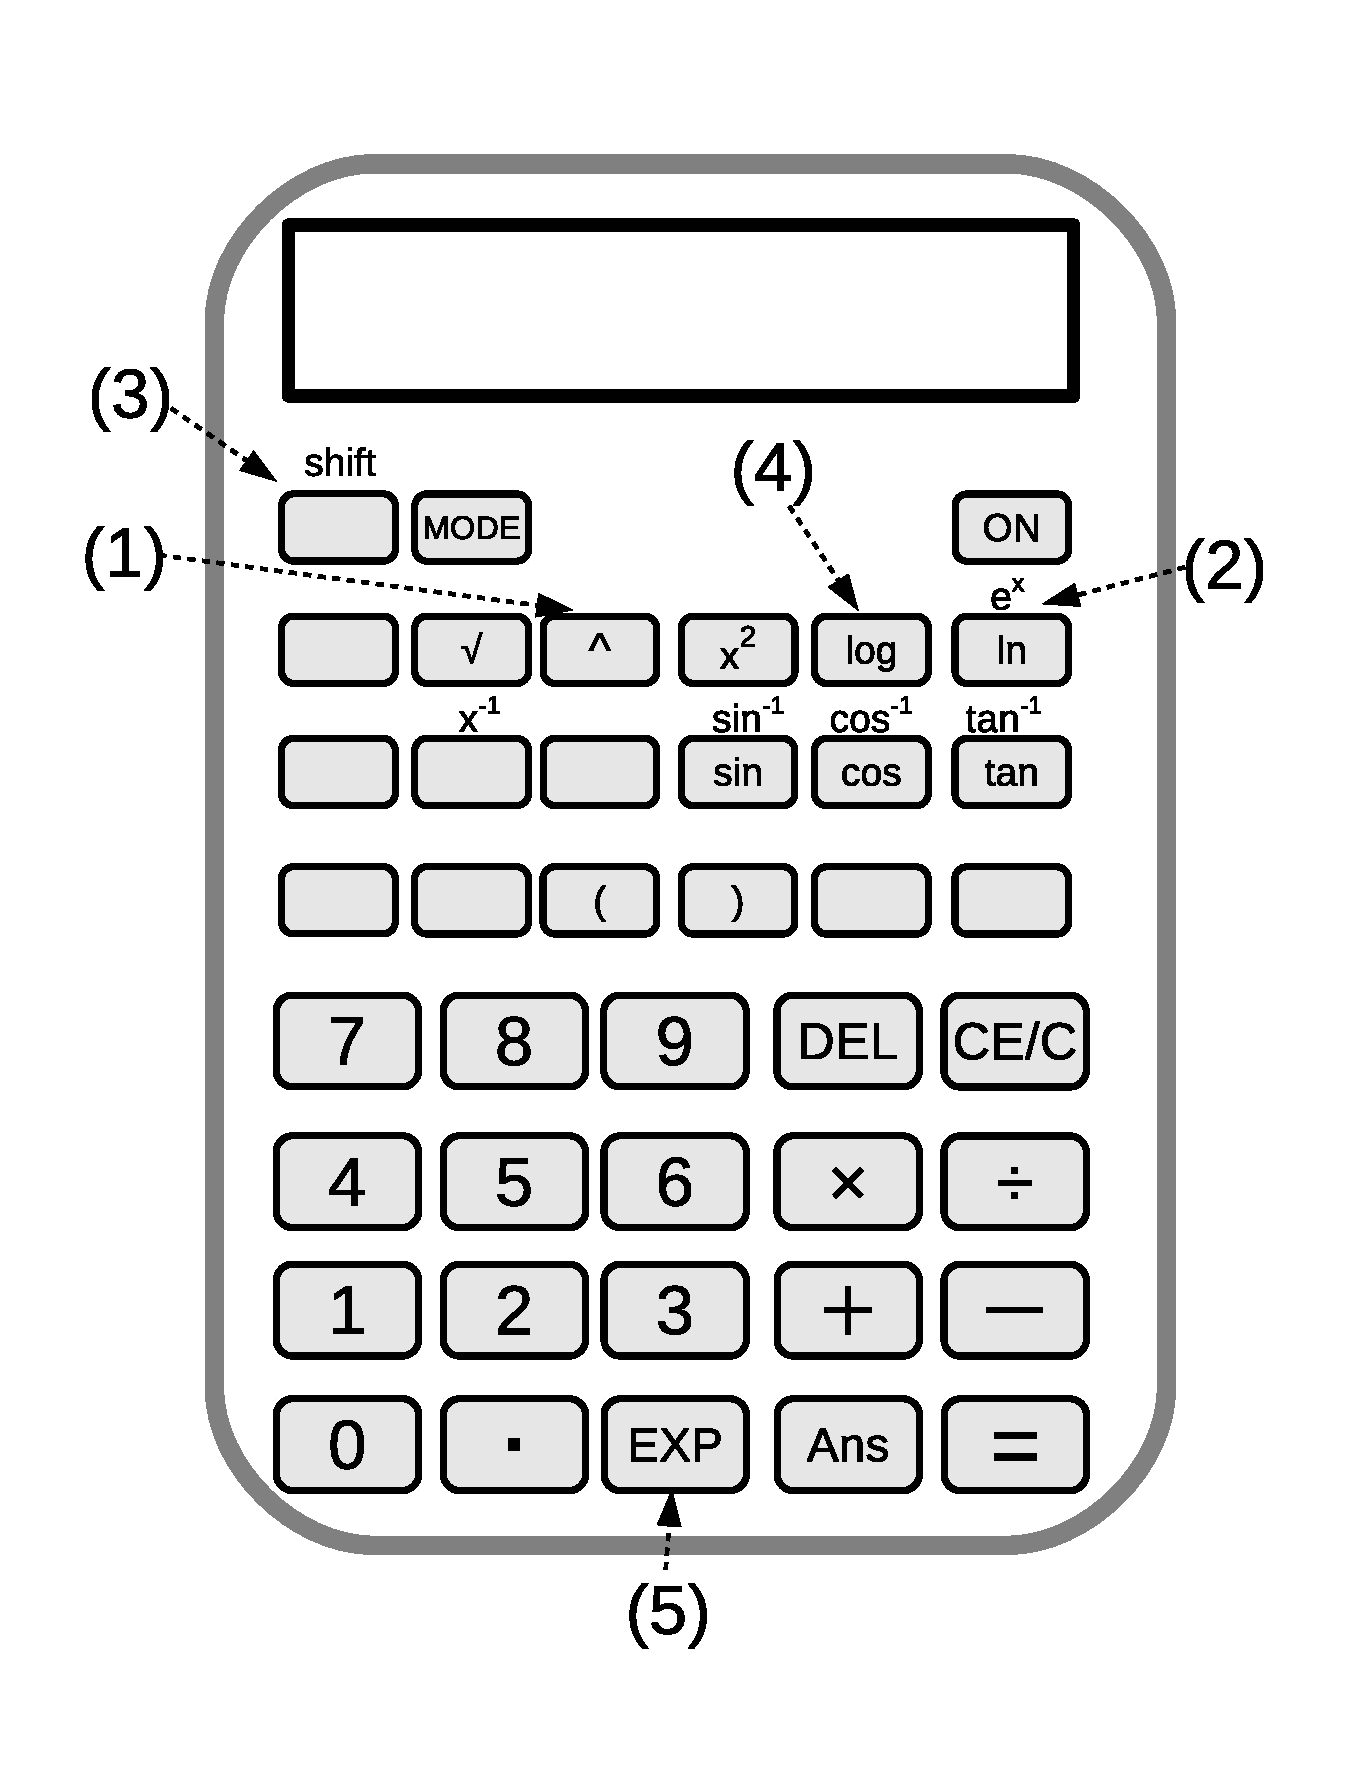
\includegraphics[width=7.5cm]{calculator.eps}
    \caption{関数電卓。普通の電卓と違って, キーがたくさん
ある。特に, (2)や(4)のキーがあるところが, 普通の電卓との違い。}\label{fig:calculator}
\end{figure}
ここでは, 例として, 
$2.3^{4.5}$を求めてみよう。

まず, 数字キーを使って2.3と
入れる。次に, 図\ref{fig:calculator}の(1)で示した, 「$\hat{\,}$」という
キーを押す(計算機の業界では, 「$\hat{\,}$」は累乗を意味する。なお, 
製品によっては, 「$\hat{\,}$」が無いものもある。その場合は, かわりに
「$x^y$」というキーを押す)。そして再び数字キーで4.5と入れる。
最後に, 右下の「=」ボタンを押そう。すると, 42.43998$\cdots$という答が
表示されるだろう。

\begin{q}\label{q:alg_dentaku2} 
以下の数を電卓で小数第5位まで求めよ。
\begin{edaenumerate}<3>
\item $2^{3.5}$
\item $1.01^{100}$
\item $\sqrt[3]{5}$
\end{edaenumerate}
ヒント: 3乗根は, 1/3乗, つまり, 0.3333333...乗。
\end{q}
\mv

\section{ネイピア数}

さて, ちょっと唐突だが, 大学では「ネイピア数」\index{ねいぴあすう@ネイピア数}
というものが頻出する。ネイピア数は無理数であり, 慣習的に$e$という記号で表す。その値は,  
\begin{itembox}{ネイピア数}
\begin{eqnarray}
e=2.71828\cdots\label{eq:NapierNum_value}
\end{eqnarray}
\end{itembox}
である(これは定義ではない。ネイピア数の定義は第\ref{chapt_exp_log}章で学ぶ)。
これには「似てないやつ」「フナひと鉢ふた鉢」等の語呂合わせがある。
この値を, 少なくとも4桁めまでは記憶せよ。\hv

\begin{q}\label{q:Napier_value_memorize} \eref{eq:NapierNum_value}
を10回書いて, 記憶せよ。\end{q}

$e$は, 数学において, $\pi$と同じくらいに重要な数だ。なぜ, どのように重要
なのかは, 後の章で学ぶ。

$x$を任意の実数として, ネイピア数の$x$乗, すなわち, $e^x$のことを, $\exp x$
と書くこともある。これも大切なことなので, 必ず記憶しよう:
\begin{itembox}{約束}
$\exp x$とは, $e^x$のこと。
\end{itembox}

関数電卓で$e^x$を求めるときは, さっきやったように, 2.71828を「$\hat{\,}$」キーで
累乗してもいいのだが, もっと正確で簡単な方法がある: 
例えば$e^4$を求めるときは, 図\ref{fig:calculator}の(3)にある「Shiftキー」を押し, 
それに続いて(2)を押す\footnote{(2)のキーは本来はlnという機能なのだが(その意味は後ほど述べる), 
直前にShiftキーが押されていると, lnという機能ではなく, ボタンの上方に
書かれた$e^x$という機能に, 一時的に変わるのだ}。そして, 数字キーで4と入れて, 
最後に=キーを押せばよい。すると, 54.598$\cdots$という答が表示されるだろう。

ただし, 製品によっては, この手順を若干, 入れ替える必要がある。すなわち, 
まず4を入れて, その後で, Shiftキー, (2)のキー(lnキー), という順序でないと
ダメなものもある。いろいろ試してみよう!

ちなみに, 電卓には図\ref{fig:calculator}の(5)のように, EXPというキーも
ある。しかし, これは, $e^x$ではないことに注意!

\begin{q}\label{q:alg_dentaku_exp} 
以下の数を電卓で小数第5位まで求めよ。
\begin{edaenumerate}
\item $\exp 2$
\item $e^{-1.5}$
\end{edaenumerate}
\end{q}

\begin{faq}{\small\textgt{関数電卓の使い方がわかりません} ... 関数電卓は
機種によって機能やデザインが違います。とりあえず, 間違えることを
恐れないで, いろいろ遊んでみよう。また, ネットで「関数電卓の使い方」
で検索してみよう。どうしてもわからなければ, 質問においで!}\end{faq}


\section{対数}

正の実数$a, b$について, 「$a$を何乗すると$b$になるか」の指数を求める
操作($a^x=b$となるような$x$を求める操作)を, 
\begin{eqnarray}
\log_a b\label{eq:taisuu00}
\end{eqnarray}
とあらわす(ただし, $a\neq 1$とする)。これを
\index{log}\underline{対数}\index{たいすう@対数} (logarithm)とよぶ(定義)
\footnote{ここで$a, b$は正としたが, これらが負であっても, 同様のことを考えることは, 
場合によっては可能である。例えば$b=-8$, $a=-2$とすれば, 「$a$を何乗すると$b$になるか」の答えは
3である。しかし, 例えば$b=8, a=-2$とか, $b=-8, a=2$とかになると, $a$を何乗しても$b$にはならない。
このような例外がたくさん生じるのは面倒なので, 対数を考えるときは, 普通, $a$や$b$に相当する数を
プラスに限定するのだ。}。\eref{eq:taisuu00}の$a$にあたる数を\underline{底} \index{てい@底}と呼ぶ。\eref{eq:taisuu00}の$b$にあたる数を\underline{真数} \index{しんすう@真数}と呼ぶ。

\begin{exmpl} 
\begin{itemize}
\item $\log_2 8=3$である。2を3乗したら8になるから。
\item $\log_2 1=0$である。2を0乗したら1になるから。
\item $\log_2 0.5=-1$である。2を$-1$乗したら1/2, つまり0.5になるから。
\end{itemize}
%(例おわり)
\end{exmpl}

\begin{q}\label{q:exp_logvalue0} 以下の値を求めよ(電卓等を使わずに):
\begin{edaenumerate}<3>
\item $\log_2 4$
\item $\log_{3} 81$
\item $\log_{0.1} 0.01$
\item $\log_{10} 1000$
\item $\log_{10} 0.01$
\item $\log_{10} 1$
\end{edaenumerate}\end{q}
\hv

10を底とする対数を\underline{常用対数} \index{じょうようたいすう@常用対数}と呼ぶ。
また, ネイピア数$e=2.718\cdots$を底とする対数を\underline{自然対数} \index{しぜんたいすう@自然対数}
と呼ぶので, ネイピア数のことを「自然対数の底」\index{しぜんたいすうのてい@自然対数の底}と
呼ぶことも多い。

\begin{q}\label{q:whatis_log} 以下の言葉の定義を述べよ:
\begin{edaenumerate}
\item 対数
\item 常用対数 
\item 自然対数
\end{edaenumerate}
\end{q}

常用対数や自然対数はよく使うので, 底を省略して$\log x$と書かれることが
世間ではよくある。その場合, 常用対数なのか自然対数なのか, 
読者が空気を読んで判断しなければならない。これはトラブルの種
であり危険な慣習である。君はこんな慣習を真似てはダメ。
常用対数なら, 面倒くさがらずに$\log_{10}x$と書くべし。一方, 
自然対数は, $\ln x$\index{ln}と書く慣習もある。lnはlog natural
の略である。これは底を誤解する余地が無く, 便利なので, 我々はこの表記を採用しよう。
\begin{itembox}{約束}
対数の底を省略しない。つまり, 常用対数や自然対数を, 
$\log x$と書いてはいけない。自然対数($\log_e x$のこと)は
$\ln x$と書いてもよい。
\end{itembox}

生物資源学類「基礎数学I, II」「物理学I」等では, 上の
「約束」を守らない答案は, \textgt{全て零点!}

\begin{freqmiss}{\small\textgt{自然対数lnをInとか1nと書いてしまう} ...
lは小文字のエルです。数字のイチや, 大文字のアイでは
ありません。手書きのときは, 筆記体($\ell$)で書こう!}\end{freqmiss}

\begin{faq}{\small\textgt{高校数学では, 自然対数は$\log x$でOK
でした。大学の他の授業や教科書も, $\log x$と書いてるのは多いです。
$\log x$と書いたら零点なんてキツすぎません?} ... 
こういう例があります: 森林科学では, 木の体積(それが木材としての商品価値を決める!)を, 
木の高さと胸高直径(人の胸の高さで測った幹の直径)で推定します。
ある論文で, その推定式が, 対数を使って書かれていましたが, 
底が省略されており, それが10なのか$e$なのか, わかりませんでした。
君ならどうしますか? 10か$e$のどちらかを適当に使いますか? 
それで間違った計算をして, まだ十分に大きくなっていない木を
切っちゃったらどうします? あるいは, 君の書く論文で対数の底が
書いてないせいで, 誰かがそういうミスをしたら, どうします?
}\end{faq}

関数電卓で自然対数を求める時は, lnというキーを使う(図\ref{fig:calculator}の(2))。
例えば, $\ln 3$を知りたかったら, lnキーを押して, その後に3を押し, =キーを押せば
よい。製品によっては逆のこともある。つまり, 先に3を押し, そのあとでlnキー, という
場合もある。

同様に, 常用対数を求める時は, logというキーを使う(図\ref{fig:calculator}の(4))。
多くの関数電卓では, logは常用対数を意味する。例えば, $\log_{10} 2$を
知りたかったら, logキー, 2, =を順に押せば良い(もしくは, 2, logキーの順)。

\begin{q}\label{q:alg_dentaku_ln} 
電卓を使って以下を小数第5位まで求めよ。\\
(1) $\log_{10} 2$ 
(2) $\log_{10} 0.006$ 
(3) $\ln 2$ 
(4) $\ln 10$
\end{q}
\mv


\section{ベクトル}\label{sect:vector_digest}

平面や空間の中で, 大きさと向きをもつ量(速度とか力とか)を
\underline{ベクトル} \index{べくとる@ベクトル}と呼ぶ。ベクトルは
物理学や化学に関連した授業で頻繁に出てくるので, ここで基本
を学んでおこう。

ベクトルは矢印で図示する。「大きさ」を
矢印の長さで表現し, 「向き」を矢印の向きで表現するのだ。

ベクトルが空間の中のどこにあるか, ということは考えない(というか, 問題にしない)。
例えば, 風速1.0~m~s$^{-1}$の風が北から南向きに吹く, という現象(風速)を
ベクトルとして表現すると, その風がどこの場所で吹いているか, ということは問題
にしない。従って, 以下に描いた3つのベクトルは, いずれも互いに等しい
ベクトルである(描かれた場所は違っても, 矢印の長さと向きは同じだから)。

\begin{center}
\setlength{\unitlength}{1mm}
\begin{picture}(60,15)
\thicklines
\put(2,8){\vector(2,1){10}}
\put(18,1){\vector(2,1){10}}
\put(36,10){\vector(2,1){10}}
\end{picture}
\end{center}

数を$a$や$x$のような記号で表すように, ベクトルも記号で表すことが多い。高校数学では
\begin{eqnarray*}\overrightarrow{a}, \overrightarrow{b}, \overrightarrow{c}, \cdots, \overrightarrow{x}, \overrightarrow{y}, \overrightarrow{z},
\overrightarrow{A}, \overrightarrow{B}, \overrightarrow{C}, \cdots, \overrightarrow{X}, \overrightarrow{Y}, \overrightarrow{Z}\end{eqnarray*}
のように, 矢印が上に載ったアルファベットで表す。しかし大学では, 
\begin{eqnarray*}{\bf a}, {\bf b}, {\bf c}, \cdots, {\bf x}, {\bf y}, {\bf z}, 
{\bf A}, {\bf B}, {\bf C}, \cdots, {\bf X}, {\bf Y}, {\bf Z}\end{eqnarray*}
のように, 太字のアルファベットで表すことが多い。手書きすると図\ref{fig:vector}のようになる。

\begin{figure}\centering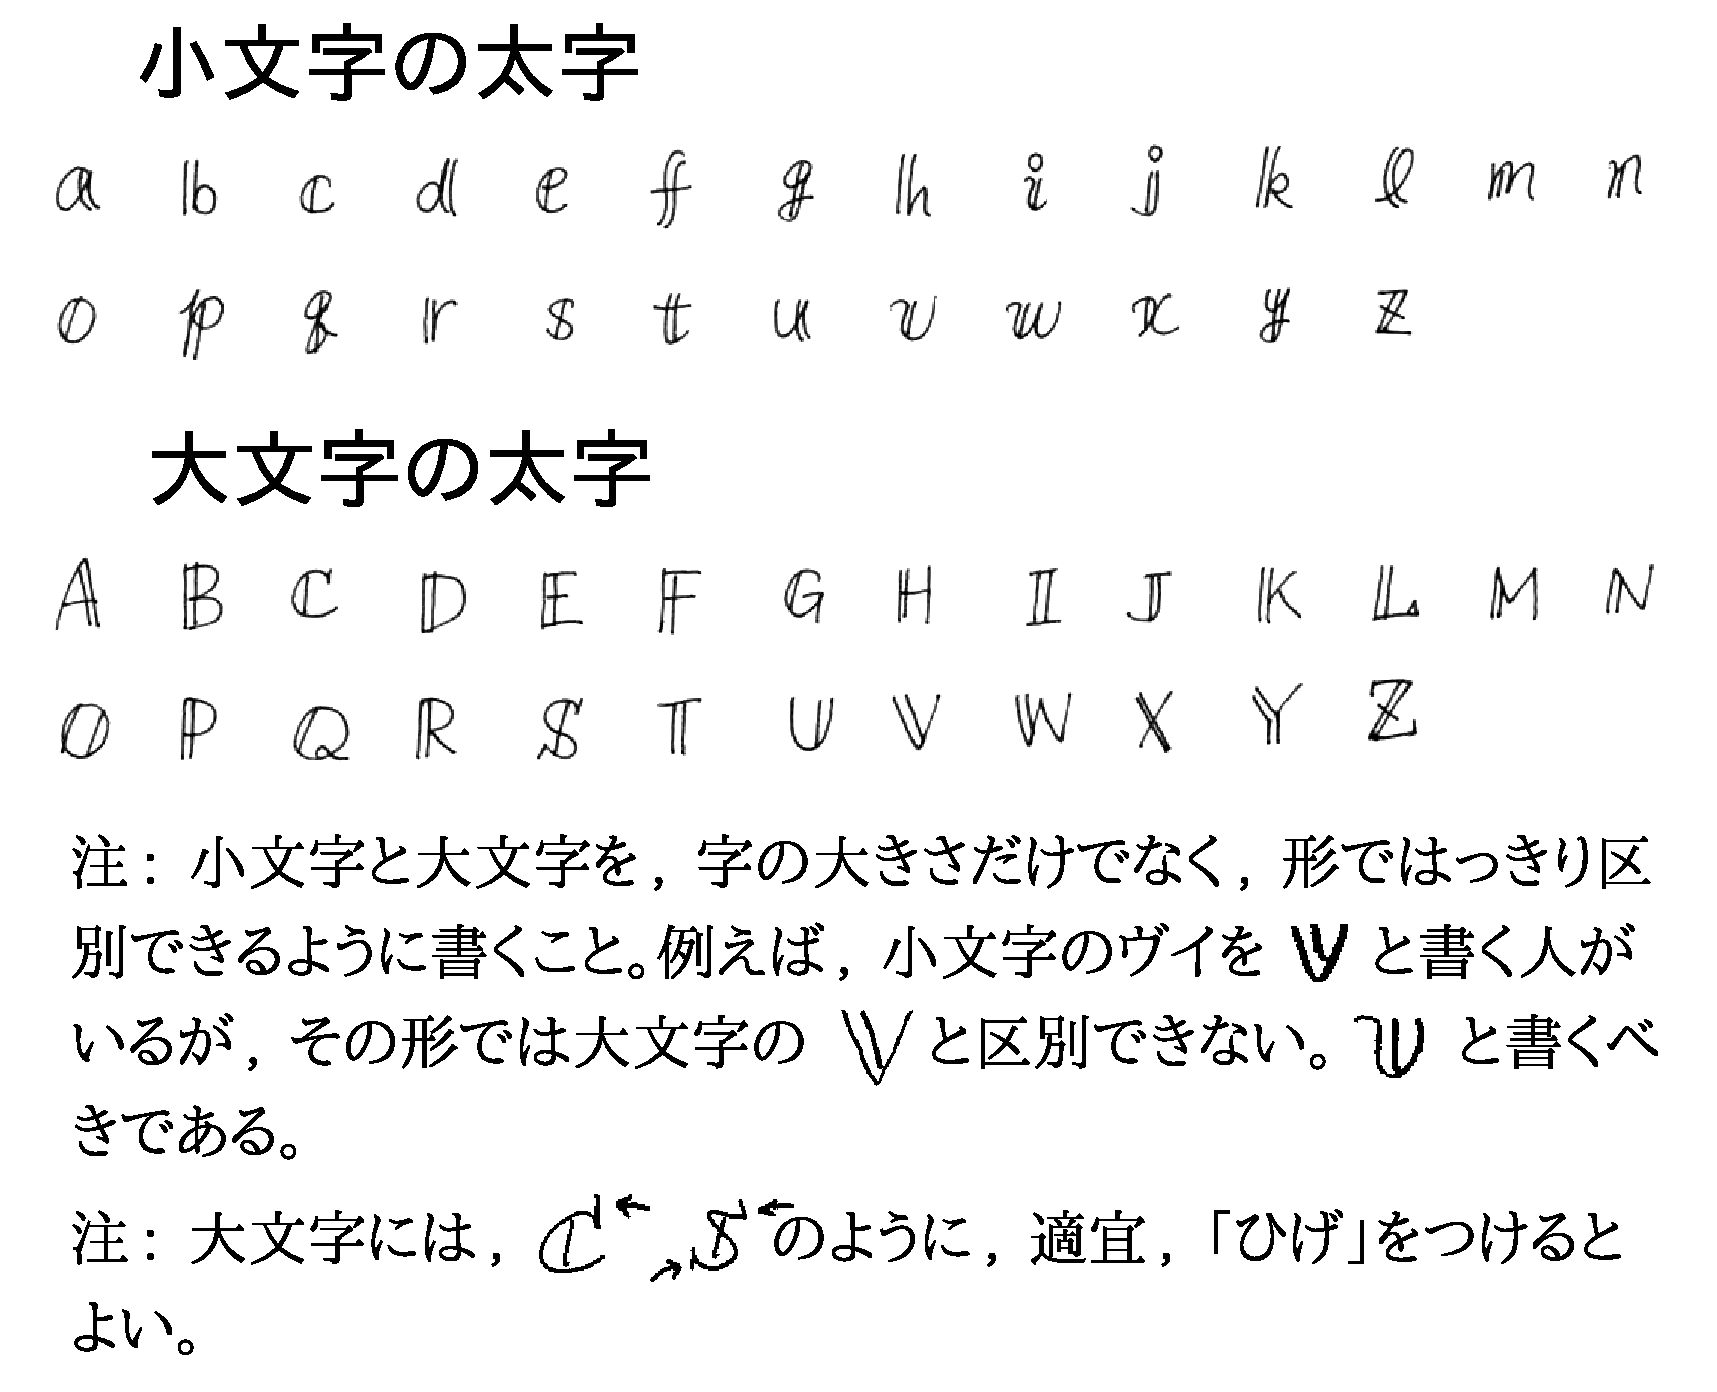
\includegraphics[width=8.0cm]{futoji.eps}

\caption{太字のアルファベットの手書き例。大切なのは, 1:太字だとわかること, 2:何の字かわかること, 
3:大文字と小文字を形で区別できること。この3つを全て満たしていれば, どう書いてもかまわない。
特に3について, 注意が必要なのは, ${\bf C}$と${\bf c}$, ${\bf O}$と${\bf o}$, ${\bf P}$と${\bf p}$, 
${\bf S}$と${\bf s}$, ${\bf V}$と${\bf v}$, ${\bf W}$と${\bf w}$, ${\bf X}$と${\bf x}$, 
${\bf Z}$と${\bf z}$である。また, ${\bf h}$と${\bf n}$も容易に紛らわしくなるので
注意。\label{fig:vector}}
\end{figure}

\begin{q}\label{q:vect_write} 図\ref{fig:vector}を参考にして, 
太字のアルファベットを全て(小文字・大文字ともに), 3回ずつ書け。\end{q}

ベクトルを記号で表すやりかたとして, もうひとつ便利なのがある。下図のように
空間に点A, Bがある場合...
\begin{center}
\setlength{\unitlength}{1mm}
\begin{picture}(40,13)
\put(2,2){\circle*{2}}
\put(31.5,11.9){\circle*{2}}
\put(30,14.5){B}
\put(1,5){A}
\thicklines
\put(2,2){\vector(3,1){29}}
\put(12,9){$\overrightarrow{\text{AB}}$}
\end{picture}
\end{center}
点Aを始点とし, 点Bを終点とするようなベクトルを扱いたいことが
よくある。そういうとき, そのベクトルを$\overrightarrow{\text{AB}}$
と書くのだ。\mv

\begin{faq}{\small\textgt{さっき, 「ベクトルが空間の中の
どこにあるか, ということは考えない」とありましたよね。でも, 
そのベクトル$\overrightarrow{\text{AB}}$は, 点Aと点B (の間)
にあります。なんか矛盾してません?} ... 確かに$\overrightarrow{\text{AB}}$は
特定の場所A, Bを使って定義されましたが, それをどの場所に持って行っても
いいのです。例えばもしも別の場所に点Cと点Dがあって, $\overrightarrow{\text{CD}}$
が$\overrightarrow{\text{AB}}$と同じ向きで同じ大きさ(長さ)なら 
$\overrightarrow{\text{AB}}=\overrightarrow{\text{CD}}$なので, 
$\overrightarrow{\text{CD}}$のことを$\overrightarrow{\text{AB}}$と
呼んでもいいのです(紛らわしいけど間違いではない)。}\end{faq}

ベクトル${\bf a}$の大きさを$|{\bf a}|$と表す。大きさが0であるような
ベクトルを${\bf 0}$と書く。すなわち$|{\bf 0}|=0$である。\\

さて, 「向きを持たず, 大きさだけを持つ量」を\underline{スカラー} 
\index{すからー@スカラー}
% (scalar)
と呼ぶ。要するに普通の実数(2とか3.14とか$-5$など)のことだ。

\begin{faq}{\small\textgt{なら, スカラーなんて言葉を使わないで, 
単に実数と呼べばいいじゃないですか?} ... それはそうですが, 
「ベクトルでない量」という意味合いを含ませるためにあえて
スカラーと呼ぶのです。}\end{faq}

$\alpha$をスカラー, ${\bf a}$をベクトルとする。${\bf a}$と同じ向きで
大きさが$\alpha$倍であるようなベクトルを, 「ベクトル${\bf a}$の$\alpha$倍」, 
もしくは$\alpha {\bf a}$と定義する。ただし, マイナス倍は, 向きを逆にする。

\begin{center}
\setlength{\unitlength}{1mm}
\begin{picture}(60,12)
\thicklines
\put(2,5){\vector(2,1){10}}
\put(5,10){${\bf a}$}
\put(18,3){\vector(2,1){20}}
\put(24,9){$2 {\bf a}$}
\put(56,10){\vector(-2,-1){10}}
\put(46,9){$- {\bf a}$}
\end{picture}
\end{center}

スカラーを表す変数は, 普通の数の変数と同じように, 細字の
斜字体で表記する。スカラーとベクトルの表記の違いをよく見比べてみよう:
\begin{itembox}{スカラーとベクトルの字体の違い}
スカラー: $a, b, c,\, \cdots,\, x, y, z, A, B, C,\, \cdots,\, X, Y, Z$\\
ベクトル: ${\bf a}, {\bf b}, {\bf c}, \cdots, {\bf x}, {\bf y}, {\bf z}, 
{\bf A}, {\bf B}, {\bf C}, \cdots, {\bf X}, {\bf Y}, {\bf Z}$
\end{itembox}
両者は見た目で明らかに違う。字の太さだけでなく, 形も違う。
この違いをよく覚えて, スカラーとベクトルを混同しないようにして欲しい。\\

\begin{freqmiss}{\small\textgt{ベクトルを普通の(矢印もつけない)細字, 
つまり$a, b, c, \cdots$等と書いてしまう} ... 
これは, 毎年, 多くの資源生が何回も何回もやらかします。あまりに深刻なので, 
大きく書いておこう!}\end{freqmiss}
\begin{itembox}{約束}
ベクトルは太字で書くか, 上付き矢印を書くこと! \textgt{単なる細字で書いてはいけない}!
\end{itembox}
%印刷物やプリントを, 注意して見よう。
%太字と細字が明確に区別されて使われていることがわかるだろう。

また, 太字で書くと決めたベクトルを上付き矢印で書いたり, その逆をしたりしてはいけない。
例えば, あるベクトルを${\bf a}$と書くと決めたなら, それを$\vec{a}$と書いてはいけない。\\

2つのベクトル${\bf a}$, ${\bf b}$が, 0でないスカラー$\alpha$によって, 
\begin{eqnarray}
\alpha{\bf a}={\bf b}\label{eq:def_parallel}
\end{eqnarray}
と書けるとき, ${\bf a}$と${\bf b}$は互いに\underline{平行}\index{へいこう@平行}
である, という(定義)。これは直感的に明らかだろう。\\

ここで, ベクトル同士の足し算(和)を定義しよう: 2つのベクトル${\bf a}$, ${\bf b}$について, 
${\bf a}$の終点に${\bf b}$の始点を置いたときに, ${\bf a}$の始点から${\bf b}$の終点まで
を結ぶベクトルを, 「${\bf a}$と${\bf b}$の和」, もしくは${\bf a}+{\bf b}$と定義する。

\begin{center}
\setlength{\unitlength}{1mm}
\begin{picture}(60,18)
\thicklines
\put(11,15){\vector(1,0){20}}
\put(18,17){${\bf b}$}
\put(2,5){\vector(1,1){10}}
\put(4,10){${\bf a}$}
\put(2,5){\vector(3,1){29}}
\put(16,8){${\bf a}+{\bf b}$}
\end{picture}
\end{center}
または, こう考えても良い:${\bf a}$, ${\bf b}$の各始点を共有させるときに, 
${\bf a}$, ${\bf b}$が張る平行四辺形の対角線(始点は各ベクトルの始点)に対応するベクトルが, 
${\bf a}+{\bf b}$である。中学校の理科でやった, 平行四辺形を使った力の合成を思い出せばよい。

\begin{center}
\setlength{\unitlength}{1mm}
\begin{picture}(60,20)
\thicklines
\put(2,10){\vector(1,0){20}}
\put(12,6){${\bf b}$}
\put(2,10){\vector(1,1){10}}
\put(4,15){${\bf a}$}
\put(2,10){\vector(3,1){29}}
\put(16,13){${\bf a}+{\bf b}$}
\thinlines
\put(11,20){\line(1,0){20}}
\put(22,10){\line(1,1){10}}
\end{picture}
\end{center}
これらの2つの考え方(定義)は, 同等である。

\begin{q}\label{q:vect_add_fig} 以下の2つのベクトル${\bf a}, {\bf b}$について, ${\bf a}+{\bf b}$, ${\bf a}-{\bf b}$, $2{\bf a} + 3{\bf b}$
を, それぞれ作図せよ。
\begin{center}
\setlength{\unitlength}{1mm}
\begin{picture}(60,19)
\thicklines
\put(27,10){\vector(2,-1){15}}
\put(37,6){${\bf a}$}
\put(12,10){\vector(1,1){10}}
\put(14,15){${\bf b}$}
\end{picture}
\end{center}
\end{q}
\mv

次に, ベクトル同士の引き算(差)を定義しよう: 2つのベクトル${\bf a}$, ${\bf b}$について, 
\begin{eqnarray*}
{\bf a}={\bf b}+{\bf x}\quad\text{を満たすベクトル${\bf x}$を求めること}
\end{eqnarray*}
を「{\bf a}から{\bf b}を引く」と呼び, ${\bf a}-{\bf b}$と書く。これは, 形式的には
\eref{eq:def_subtract}とほとんど同じだ。図では以下のようになる:

\begin{center}
\setlength{\unitlength}{1mm}
\begin{picture}(60,22)
\thicklines
\put(20,10){\vector(2,-1){15}}
\put(25,3){${\bf b}$}
\put(20,10){\vector(1,1){10}}
\put(22,15){${\bf a}$}
\put(35,4){\vector(-1,3){5}}
\put(35,10){${\bf a} - {\bf b}$}
\end{picture}
\end{center}

初心者はこの話で, ${\bf a}-{\bf b}$の向きを混乱することがよくある。
${\bf a}-{\bf b}$の終点は${\bf a}$(の終点)であり, 
${\bf a}-{\bf b}$の始点は${\bf b}$(の終点)である。
これを縮めて, 「ベクトルの引き算は終点引く始点」と覚えるとよい。\\

さて, ベクトルを表す時にいつも矢印を作図するのは面倒くさくて仕方ない。
そこで便利なのが「座標」という考えである。これは, \fref{fig:vector_coordinate}
のように, ベクトルを座標平面($x$軸と$y$軸があるような平面)の
上に, 始点が原点Oに来るように\footnote{原点をあらわすOは「零」ではない。
originの頭文字の「オー」の大文字である。}置き, 終点(矢印の先端)から$x$軸と
$y$軸のそれぞれに垂直に線をおろして(方眼紙のように), 
原点からそれぞれへの長さを, $(3, 2)$のように並べたものである。

\begin{figure}
    \centering
    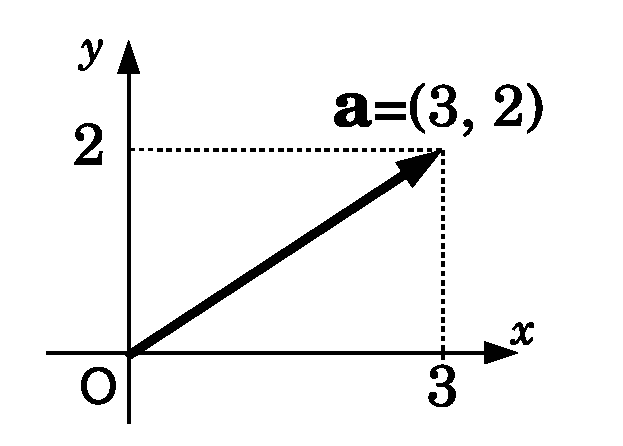
\includegraphics[width=4cm]{vector_coordinate.eps}
    \caption{ベクトルを座標で表す。\label{fig:vector_coordinate}}
\end{figure}

これは平面上のベクトルの場合だが, 空間のベクトルの場合は, さらに
高さ方向の軸($z$軸)があるような座標空間を考えて, $(3, 2, 1)$のように
3つの数値を並べることで表現できる。こういうのを「座標」と呼ぶ。
ベクトルは矢印で表しても, 座標で表してもよいのである。\\

座標の利点は, 「計算が楽」ということだ。あるベクトルをスカラー倍したり
ベクトル同士を足したり引いたりするとき, 矢印ならいちいち作図しなければ
ならないが, 座標なら数値の計算で済む。

\begin{exmpl} ${\bf a}=(1, 2)$と${\bf b}=(-3, 4)$について, 
$5{\bf a}+{\bf b}$は?\\
$5{\bf a}+{\bf b}=5(1, 2)+(-3, 4)=(5\times1-3, 5\times2+4)=(2, 14)$
(例おわり)\end{exmpl}

\section{位置ベクトル}

前述したように, ベクトルは大きさ(長さ)と向きを持つ量であり, 本来は, 
それが空間のどこにあるかは問わない。でも, 空間内のどこかに原点O
を定めれば, 空間内の点Pの位置は, ベクトル$\overrightarrow{\text{OP}}$
によって表現できる。このように, 空間の点の位置を表すベクトルのことを, 
\underline{位置ベクトル} \index{いちべくとる@位置ベクトル}という。
位置ベクトルを考えるときは, 空間内のどこかに原点があって, そこを始点とするベクトルを
考えているのだという意識を持とう。ただし, その原点が具体的にどこなのかは, 
多くの場合は問題にされない。どこかは知らなくても, どこかにあるのだ。

位置ベクトルは, 次の例のように使う:

\begin{exmpl} 空間内に2つの点A, Bがあり, それぞれの位置ベクトルを${\bf a}$, ${\bf b}$
とする。その意味は, どこかに適当な原点Oがあって(どこでもよい), ${\bf a}=\overrightarrow{\text{OA}}$, 
${\bf b}=\overrightarrow{\text{OB}}$である, ということだ。このとき, 
$\overrightarrow{\text{AB}}={\bf b}-{\bf a}$である(なぜかは各自
考えてみよう)。また, 線分ABの中点Cの位置ベクトル${\bf c}$は(${\bf c}$は
$\overrightarrow{\text{OC}}$のこと), 
\begin{eqnarray}
{\bf c}=\frac{{\bf a}+{\bf b}}{2}\label{eq:vect_middlepoint}
\end{eqnarray}
である(なぜかは各自考えてみよう)。

では, 線分ABを$m:n$に内分\index{ないぶん@内分}する点P (つまり, 線分AB上にあって, 
AP:PB$=m:n$になるような点P)は, どこにあるだろうか? Pの位置ベクトルを$\bf p$
としよう(図\ref{fig:vector_3})。明らかに, 
\begin{eqnarray}
{\bf p}&=&\overrightarrow{\text{OA}}+\overrightarrow{\text{AP}}={\bf a} + \frac{m}{m+n}\overrightarrow{\text{AB}}={\bf a} + \frac{m}{m+n}({\bf b}-{\bf a})\nonumber\\
&=&\frac{n {\bf a} + m {\bf b}}{m+n}\label{eq:vect_naibun}
\end{eqnarray}
となる。この式の右辺で$m=n=1$とすると\eref{eq:vect_middlepoint}の右辺に一致する!
\begin{figure}[h]
    \centering
    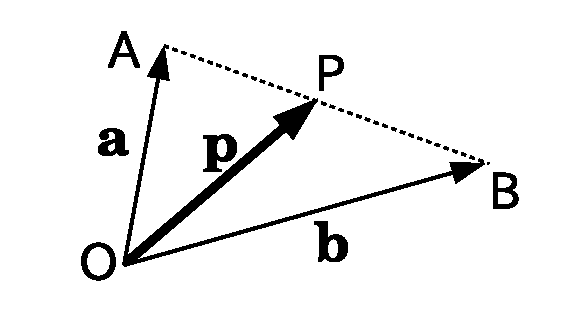
\includegraphics[width=4cm]{vector_3.eps}
    \caption{点Aと点Bの間を内分する点P。\label{fig:vector_3}}
\end{figure}
(例おわり)\end{exmpl}

\begin{q}\label{q:vect_pos2D} 点A, Bの位置ベクトルがそれぞれ(4, 5)と(3, 6)であるとき, 
\begin{enumerate}
\item ABを1:2に内分する点の座標を求めよ.
\item ABを2:1に内分する点の座標を求めよ.
\end{enumerate}\end{q}\mv


\begin{faq}{\small\textgt{ベクトルは太字よりも
上付き矢印を使ったほうが分かりやすいです。}
... そのうち太字に慣れますよ。}\end{faq}

\begin{comment}
ここで書き方に関する注意。問\ref{q:vect_pos2D}のように, A(1, 2)と
書くときは, Aは点の名前(ラベル)であり, (1, 2)は点の座標である。
そして, この点の位置ベクトルを${\bf a}$とすると, ${\bf a}=(1, 2)$
と書く。ところが, これを, ${\bf a}(1, 2)$と書く人がいる。\textgt{これはよくない}。
${\bf a}$と$(1, 2)$の間には, 必ず等号を書かねばならない。
というのも, 
数学では, ${\bf a}(1, 2)$は${\bf a}=(1, 2)$とは違った意味を持つ
のである\footnote{平面上の全ての点にひとつずつベクトルが存在する
ような数学的概念を考えると, それは${\bf a}(x, y)$のように表される。
その場合, 点(2, 3)\textgt{における}ベクトルを${\bf a}(2, 3)$
のように表す(これはちょうど, 関数$f(x)$について, $x=4$での
値が$f(4)$である, というのと同じような括弧の使い方である)。
このとき, (2, 3)は, そのベクトルがある場所を表すのであり, 
そのベクトルそのものを表すのではない。だから, もしかしたら
${\bf a}(2, 3)=(1, 2)$かもしれないし, ${\bf a}(2, 3)=(0, 0)$
かもしれない。}。
\end{comment}
\mv



\section{有効数字}

現実的な話題で出てくる数値の多くは, 誤差を持つ。

例えば, 総務省統計局によると, 平成27年2月1日現在, 日本の総人口は, 
「1億2697万人」らしい。この推計値に「1万人」の桁までしかないことに
注意しよう。本当は, 1億2697万5678人とか, 1億2697万1212人
のように, 万よりも小さな桁にも何か数があるはず。でも, 誤差のために, 
そこまでの詳しい数は出せないのだ。というのも, 日本では, 1日に約3千人
(約30秒に1人)のペースで赤ちゃんが生まれるし, 同じくらいのペース
で人が亡くなっている。それらの人の生死は等間隔で起きるわけではないし, 
起きてすぐに総務省に報告が来るわけでもないから, 誤差ゼロで
人口を推計することはほぼ無理だし, 意味ないのだ。

そこで, 上の「1億2697万」という数は, 億から万までの位の数字, 
つまり, 1, 2, 6, 9, 7だけが意味あると考える。このように, 
誤差を含む数値において, 意味のある数字のことを
「有効数字」\index{ゆうこうすうじ@有効数字}と呼ぶ。そして誤差は, 
有効数字の中で, 最も小さな位の数(上の例では7)に影響する程度
だろうと考える。従って, 最も小さな位の数は, 信用できない(意味がない)
わけではないが, ちょっと怪しいぞ(上の例では, 7が6とか8になってもおかしく
ないかも), と疑ってかかるのだ(つまり, 怪しい数字の最大の位が
有効数字の最小の位である)。\\

誤差のある数値を扱う時は, 常に有効数字を意識しよう。まず, 
数値の有効数字がどの桁までなのかをはっきりさせよう。
そのときに注意が必要なのは「0」という数字の扱いである。

例えば, 「A君, 今, いくら持ってる?」という問に, A君が「だいたい1200円」
と答えたとする。このとき, おそらく真実は1100円から1300円くらい
の間にある(誤差は100円くらい)と考えるのが常識的な判断だろう。この場合, 
有効数字は1と2の2桁であり, それよりも下の2桁の0は, 有効数字ではなく, 
位取りのため(数値の桁を表現するため)の0であるにすぎない。ところが, 
A君は実際は几帳面な人で, 10円単位で財布の中身を把握
していたとするなら, A君の「だいたい1200円」
の意味するところは, 1190円から1210円くらい, ということになる。その場合, 
1, 2だけでなく, その次の0(つまり10円の位の0)も, 有効数字である。

つまり, 0という数字は困ったもので, 「位取りの0」と「有効数字の0」という
2つの異なる役割を担う。それが紛らわしくて, 数値を見ただけでは判断
できないのだ(そういう意味では, 上の人口の「1億2697万人」
の例でも, ホントは有効数字の0が万よりも小さな位, 例えば千とか
百にもあったかもしれない)。

ところが, 小数点が現れると, 有効数字がはっきりすることがある。例えば, 
100.0という表現を考えよう。これは数学的には100と同じ。
だから, 100.0なんて書かずに, 100と書けば良いように思う。
実際, 小数点より右側には, 位取りのために末尾(右端)に0を付け加える
必要は無い。にもかかわらず, わざわざ100.0というふうに小数点の右側
に0がある場合, この0は位取りの0ではなく, 有効数字の一部であると
解釈するしかない。すると, それよりも大きな位の数は, 全部有効数字の
はずである。従って, 100.0は, 1, 0, 0, 0という4つの数が有効数字
である, つまり有効数字は4桁である, と自信を持って判断できるのだ。
ところが, 単に100と表していたら, 自信を持って有効数字であると
判断できるのは最初の1だけだ。

では例えば, 0.0012の有効数字はどれだろうか? 1, 2は当然, 有効数字である。
しかし, それより上位にある3つの0は, 小数の位取りを表す0と考えるのが
適当である。従って, 0.0012の有効数字は, 1と2の2桁である。\\

\begin{q}\label{q:guard_digit_order} 以下の数のそれぞれについて, 
有効数字を指摘せよ。
\begin{edaenumerate}<4>
\item $5.3$
\item $1230.5$
\item $5300$
\item $0.0230$
\end{edaenumerate}
\end{q}

このように, 有効数字は, 表現法によっては曖昧になってしまう。
有効数字をはっきりさせたいときは, 数値をあえて小数を使って
書く。つまり, 小数×「10の累乗」の形で書くのである。例えば, 1200円を, 
\begin{eqnarray}
1.2\times10^3\,\text{円}\label{eq:1200yen3}\\
\text{とか, }\nonumber\\
1.20\times10^3\,\text{円}\label{eq:1200yen4}
\end{eqnarray}
というふうに書くのだ。\eref{eq:1200yen3}の場合は有効数字は1と2だけ(100円の位まで意味がある)
だが, \eref{eq:1200yen4}の場合は有効数字は1, 2, 0となる(10円の位まで意味がある)。
数学的には, $1.2\times10^3$と$1.20\times10^3$は同じなのだが, 
現実世界において誤差を含む数としては, これらは別物なのである。\\



\section{有効数字の計算}

では, 有効数字を計算(四則演算)の中でどのように扱うかを述べる。

例として, 4.56と1.2という数値の和を考える。それを筆算でやってみよう。
その際, 「怪しい数」を以下のように追跡する: まず, 
4.56は有効数字3桁で, 最後の6がちょっと怪しいのでその6を○で囲って
おこう。1.2は有効数字2桁で, 最後の2がちょっと怪しいのでその2を
□で囲っておこう。さて, 怪しい数が足されて得られた数は, 怪しさが
「伝染」してくるはずなので, その数も, ○または□で囲う。どちらの形で
囲うかは, その怪しさが伝染してきたもとの数を囲う形で決める。
ただし, 怪しい数からの繰り上がりによって受ける影響は
無視する(怪しくないとみなす)。

すると, 図\ref{fig:guard_digit_plus}のようになる:
\begin{figure}[h]
    \centering
    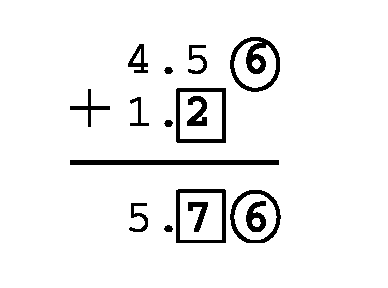
\includegraphics[width=3cm]{guard_digit_plus.eps}
    \caption{誤差を含む数どうしの和。怪しい数を○や□で囲って
ある。}\label{fig:guard_digit_plus}
\end{figure}

有効数字を考えなければ, 結果は5.76になる。最初の(1の位の)5は怪しくないが, その右(0.1の位)
の7は, 1.2の最小位の有効数字の怪しさの影響を受けているから, 怪しい。
この時点で, さらに右の6はあまり意味が無い。なぜなら, 0.1の位の7が, 
6とか8かもしれないなら, それよりも詳細な(桁の小さい)情報にこだわっても
仕方が無いからである。というわけで, この答の有効数字は, 最初の5と
次の7の2桁と考えるのが妥当だろう。そこで, 3桁目の6を切り捨てるか
切り上げよう。このように, 無意味な桁を切り捨てたり切り上げたりすることを
「丸める」\index{まるめる@丸める}という。多くの場合は, 四捨五入に
よって丸めるので, ここでは6を切り上げて最終的な答を5.8
としておこう。しかし, 「常に四捨五入が正しい」
というわけではなく, 場合によっては値によらず切り上げたり切り捨てたり
する方が妥当なこともある。

\begin{faq}{\small\textgt{「怪しい」とか「妥当だろう」とか「としておこう」
とか, なんかテキトーというか、いい加減なかんじですね。。。}
... そうです。後で述べるように, 有効数字というのは, テキトーでイイカゲン
なものなのです。}\end{faq}

このように, 足し算では, 最終的な答の有効数字は, 次のような手順で
決める: まず, 足す前の数の有効数字の最小(右端)の位をチェック。
上の例では「4.56」の右端は0.01の位であり, 「1.2」の右端は0.1の
位だ。次に, それらの中で, 最も大きな位に注目する。上の例では, 
0.1と0.01の比較となり, 大きいのは0.1の位である。その位を, 
最終的な答の有効数字の最小の位とする。上の例では, 5.76のうち, 
有効数字は0.1の位まで, つまり5と7が有効数字となる。そして, 
それより1つ小さな位を丸める。上の例では0.01の位の数, すなわち6を
四捨五入すると切り上がって, 5.8となる。こうして最終的な値を確定する。

ここでは詳しくは述べないが, 引き算も同様だ。引く数と引かれる数の
それぞれについて有効数字の最小位をチェックし, 最小位の大きい方を
最終結果の有効数字の最小位とし, それよりも1桁小さな数を丸めればよい。

\begin{q}\label{q:guard_digit_prac2} 以下の計算を行え。ただし, 
これらはいずれも誤差を含む数値とし, 有効数字に気をつけて, 無意味な
数を書かないように気をつけよ。電卓を使ってよい。丸めは四捨五入で行え。
\begin{edaenumerate}
\item $5.3 + 6.6$
\item $0.023 + 123.5$
\item $100.2 - 13$
\end{edaenumerate}
\end{q}

こんどは, 4.56と1.2の積を考えよう。それを筆算でやってみよう。
先ほどの和の例と同様に, 「怪しい数」を追跡する。すると, 
図\ref{fig:guard_digit_mult}のようになる:

\begin{figure}[h]
    \centering
    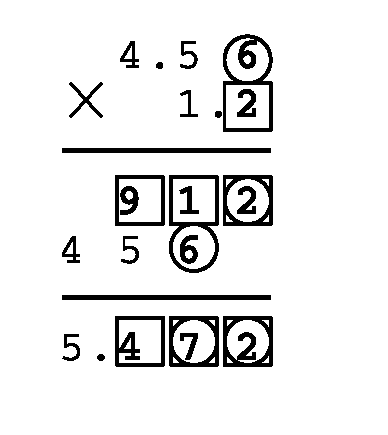
\includegraphics[width=3cm]{guard_digit_mult.eps}
    \caption{誤差を含む数どうしの積。怪しい数を○や□で囲って
ある。例えば, 3段目の9, 1, 2は, 右端の2が1段目の6の怪しさと
2段目の2の怪しさの両方の影響を
受けているので, ○と□の両方で囲ってある。}\label{fig:guard_digit_mult}
\end{figure}

有効数字を考えなければ, 結果は5.472になる。最初の(1の位の)5
は怪しくないが, その右(0.1の位)の4は怪しい。この時点で, 
さらに右の7や2はあまり意味が無い。なぜなら, 
0.1の位の4が, 3とか5かもしれないなら, それよりも詳細な(桁の小さい)
情報にこだわっても仕方が無いからである。

というわけで, この答の有効数字は, 最初の5と次の4の2桁と考えるのが
妥当だろう。そこで, 3桁目の7を切り捨てるか切り上げる。ここでは
四捨五入によって7を切り上げて最終的な答を5.5としておこう。

このように, 掛け算では, 最終的な答の有効数字は, 次のような手順で
決める: まず, 掛ける前の数の有効数字の桁数をチェックする。上の例
では「4.56」の3桁と, 「1.2」の2桁である。次に, それらの中で, 最も
小さな有効数字桁数に注目する。上の例では, 3桁と2桁の比較となり, 
最小は2桁である。その桁数を, 最終的な答の有効数字の桁数とする。
上の例では, 5.472のうち5と4の2桁が有効数字, となる。そして, 
最小の有効数字(上の例では4)よりも1桁小さな数値を丸め(上の
例では四捨五入の結果, 7が切り上がって4が5になる), 最終的な数を確定する。

ここでは詳しくは述べないが, 割り算も同様。割る数と割られる数の
それぞれについて有効数字の桁数をチェックし, 桁数の小さい方を最終結果
の有効数字の桁数とし, それよりも1桁小さな数を丸めればよい。

\begin{q}\label{q:guard_digit_prac4} 以下の計算を行え。ただし, 
これらはいずれも誤差を含む数値とし, 有効数字に気をつけて, 無意味な
数を書かないように気をつけよ。電卓を使ってよい。丸めは四捨五入で行え。
\begin{edaenumerate}
\item $5.3\times 2.6$
\item $0.023\times 123.5$
\item $100.2 / 13$
\end{edaenumerate}
\end{q}

\begin{exmpl} 長さ16 cmの棒を3等分したとき, 1本の長さは? 
小数で表せば, (16 cm)/3=5.333$\cdots$ cm。このとき, 
「16 cm」の有効数字は2桁なので, 結果の有効数字も2桁で
よかろう。3桁目を四捨五入し, 「5.3 cm」が妥当な答だろう。
 ... ちょっと待て! 「3等分」の「3」は有効数字1桁では? なら, 
結果も有効数字1桁, つまり「5 cm」が正しいのでは? と思った人
がいるかもしれない。でもそれは違うのだ。棒を3本に分けよ, 
と言われて「うっかり3.1本に分けちゃいました」なんてことは
あり得ない。つまり, この「3」の誤差は, 半端な小数ではなく, 
0, 1, 2などの整数のはず。でも, よほどのうっかり屋さんでも
3本を2本や4本に間違えることはなかろう。従って, この場合
の誤差は0。つまり, 「3本」は, 実は3.0000$\cdots$本, 
つまり有効数字が無限にある(小数点以下に有効数字の0が
無限に続く)と考えるのが妥当なのだ。従って, この割り算の
有効数字は, 「割られる数」である「16 cm」の有効数字の桁数
で決まるのだ。

ここで, 「小数にせずに, $\frac{16}{3}$ cmというふうに分数のまま
にしておけばいいじゃないか」と思う人もいるだろう。数学的にはそれで
正解である。でもこれが, 機械工作等の実務だったらどうだろうか? 
「$\frac{16}{3}$ cm」よりも「5.3 cm」の方が, ものさしで測りとる
のは簡単なので, 実務的な現場では, 数値は分数でなく
小数で表しておきたい, ということがよくあるのだ。(例おわり)\end{exmpl}



ここで注意。有効数字というのは, 実は, あまり厳密な考え方ではない。

\begin{exmpl} $3.47\times2.88$を考えよう。有効数字を考えなければ, \\
$3.47\times2.88=9.9936$\\
となる。3.47も2.88も有効数字3桁だから, 結果の有効数字は3桁のはず。
なので, 4桁目(3)以降を丸めて, 
$3.47\times2.88=9.99$\\
となる。ところが, この計算と微妙に違う, $3.47\times2.89$を考えよう。
有効数字を考えなければ, \\
$3.47\times2.89=10.0283$\\
となる。3.47も2.89も有効数字3桁だから, 結果の有効数字は3桁, ということで, 
4桁目以降(283)を丸めて, 
$3.47\times2.89=10.0$\\
となる。ここで, 変な気がしないだろうか? これらの2つの計算は, 
ほとんど同じような数値を扱っている(2.88が2.89に変わっただけ)。
ところが, 結果の有効数字は, 前者(9.99)では0.01の桁まであったのに, 
後者(10.0)では0.1の桁までしかない。つまり, 後者の誤差は前者の
誤差の10倍!? (例おわり)\end{exmpl}

こういうのが有効数字の弱点である。上述の「積の有効数字の
扱い方」を厳密に適用すると, 繰り上がりが発生する瞬間に, 
いきなり有効数字が1桁, 引き上げられてしまい, 誤差が突然に
10倍になる, という, 本来は起きるはずのないことが
起きてしまうのだ。

本来, 誤差のある数は, その誤差も明示的に表記するのが
科学的に正しい態度だ。例えば, 3.47の誤差が0.01程度
であるとわかっていれば, 「3.47$\pm0.01$」と書くべき。
そして, 計算の中で, そのように表された誤差もきちんと追跡
すれば(そのやり方は後の章で学ぶ), 変なことは起きない。

でもそれは結構面倒くさい。だから, 誤差の大きさの追跡
はサボって, 「有効数字」で勘弁してもらうのだ。そういう状況で
「有効数字は3桁? 4桁?」と考えすぎるのは不毛である。
そんなことに悩むくらいなら, 1桁余分に多くとっておくか, 
あるいは真剣に誤差の大きさを追跡するべきだ。\\

それでもあえて「有効数字」にこだわりたければ, 上の例について言えば, 
掛け算における有効数字の扱い方をここでは緩めて, $3.47\times2.89=10.0283$を, 
暫定的に有効数字4桁として, $10.03$とするのが良いように私は思う。
君はどう考えるだろうか?\\


\begin{q}\label{q:guard_digit_8} 長さ6.4~cmの棒が2本ある。これを
繋ぎあわせて1本の棒にしたら, 長さは何cmか?
\begin{enumerate}
\item 6.4 cm + 6.4 cm =という計算で, 有効数字に気をつけて, 答えを求めよ。
\item 6.4 cm $\times 2$=という計算で, 有効数字に気をつけて, 答えを求めよ。
\item これらの答の有効数字の桁数が違うことを, どのように解釈すればよいか?
\end{enumerate}
\end{q}

ところで, 例えば4.2という値(有効数字)は, 実際のところ, どのくらいの範囲の
値を意味するのだろうか?よくあるのが, 「4.15以上4.25未満」という説明である
(末尾を四捨五入して4.2になる範囲)。実はそうとも限らないのだ。「4.1以上4.3未満」や, 
「4.0以上4.4未満」であっても, 4.2という有効数字で表現してよいのだ。

「なぜ!?」と思う人には逆に聞こう。「4.1以上4.3未満」を有効数字で表すのに, 4.2
以外にどのような適切な表現があるだろう? 4.1や4.3は偏っているからダメだし, 
4や5は論外である。なら, 4.2しか無いではないか!?

\begin{q}\label{q:guard_digit_9} 以下の数値を, 「$\pm$いくら」を使わずに, 
有効数字で表すとどうなるか?
\begin{edaenumerate}<3>
\item 13.2$\pm 0.1$
\item 13.2$\pm 0.2$
\item 13.2$\pm 0.6$
\end{edaenumerate}
\end{q}

このように, 「有効数字」は, おおざっぱな考え方である。だから「有効数字を
何桁にするのが正解か?」というのは, あまりこだわっても仕方ないのだ。

\begin{faq}{\small\textgt{でも高校の物理や化学では, 有効数字の
桁数を1つでも間違えたら減点されました} ... 大事なのは, あなた自身がどう
考えるかです。あなたが「正しい」と確信することにダメ出しされたなら, 
その相手と議論すればよいのです。それが学問です。
}\end{faq}
\hv

\section{ギリシャ文字}\index{ぎりしゃもじ@ギリシャ文字}

数学では, 数や概念を表すのに, たくさんの記号を必要とする。とりあえず
英語のアルファベットだけでは足りないので, ギリシア文字もよく使う。
以下に, 特によく使うギリシア文字を示す。手書きでの書き方も含めて, 
君は必ずこれらを記憶せよ。

\begin{q}\label{q:logic_Greece}
図\ref{fig:Greece1}, 図\ref{fig:Greece2}, 図\ref{fig:Greece3}, 図\ref{fig:Greece4}
に出ているギリシア文字を全て, 3回ずつ書け。
\end{q}


\begin{figure}[H]
    \centering
    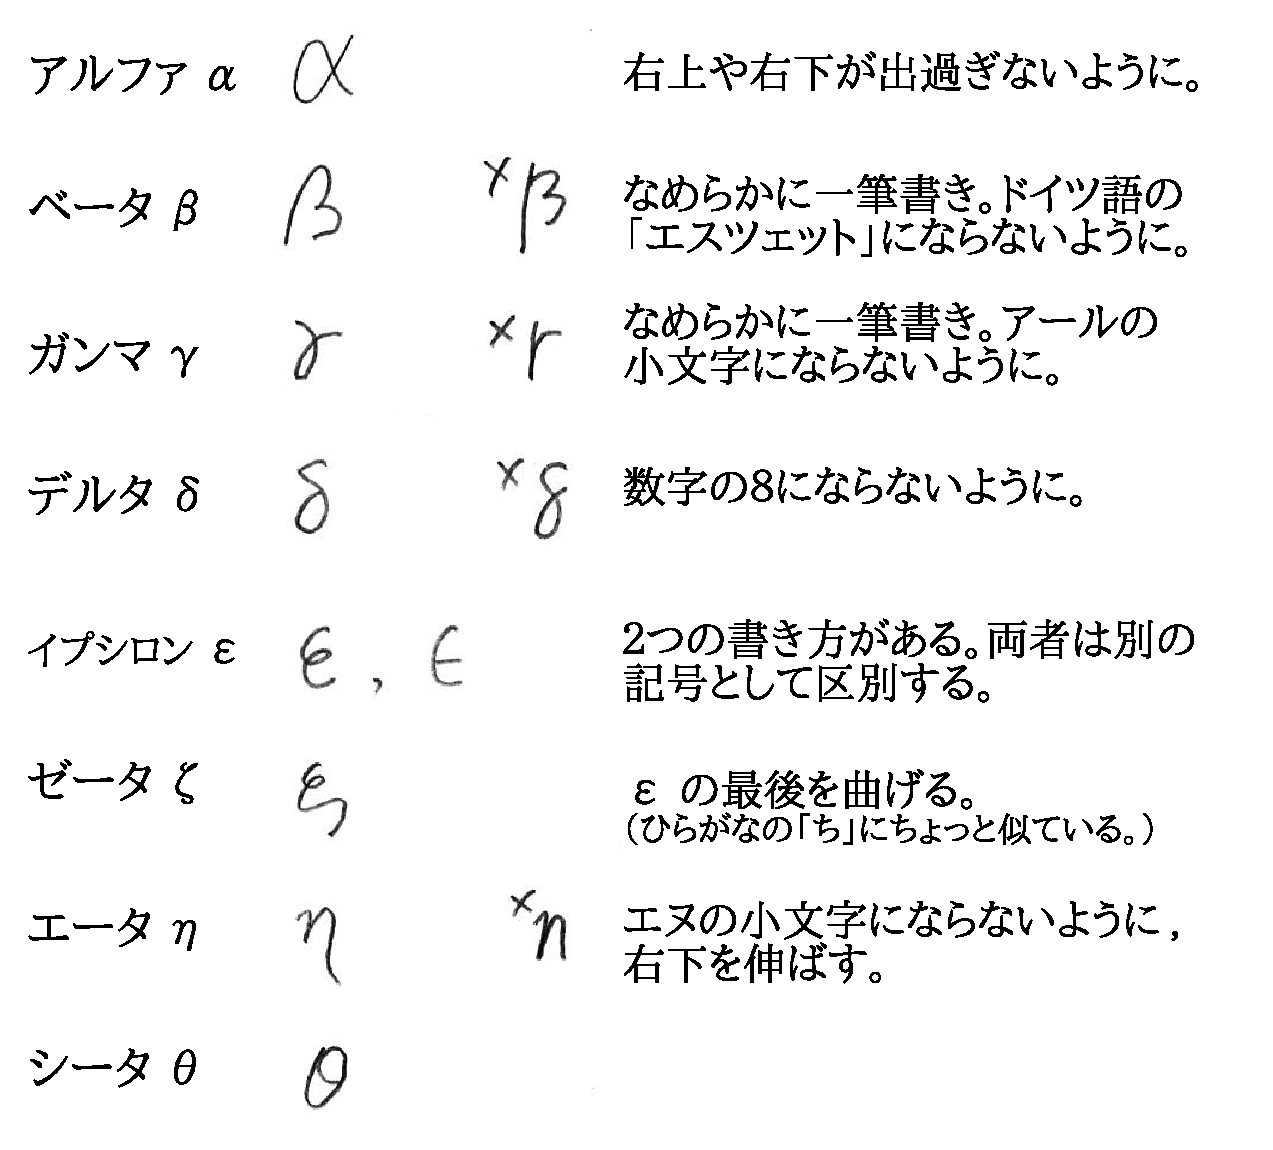
\includegraphics[width=7.5cm]{Greece1.eps}
    \caption{ギリシア文字の小文字($\alpha, \beta, \gamma, \delta, \epsilon, \zeta, \eta, \theta$)の書き方。$\times$がついているのは, よくある間違った書き方。\label{fig:Greece1}}
\end{figure}

\begin{figure}[H]
    \centering
    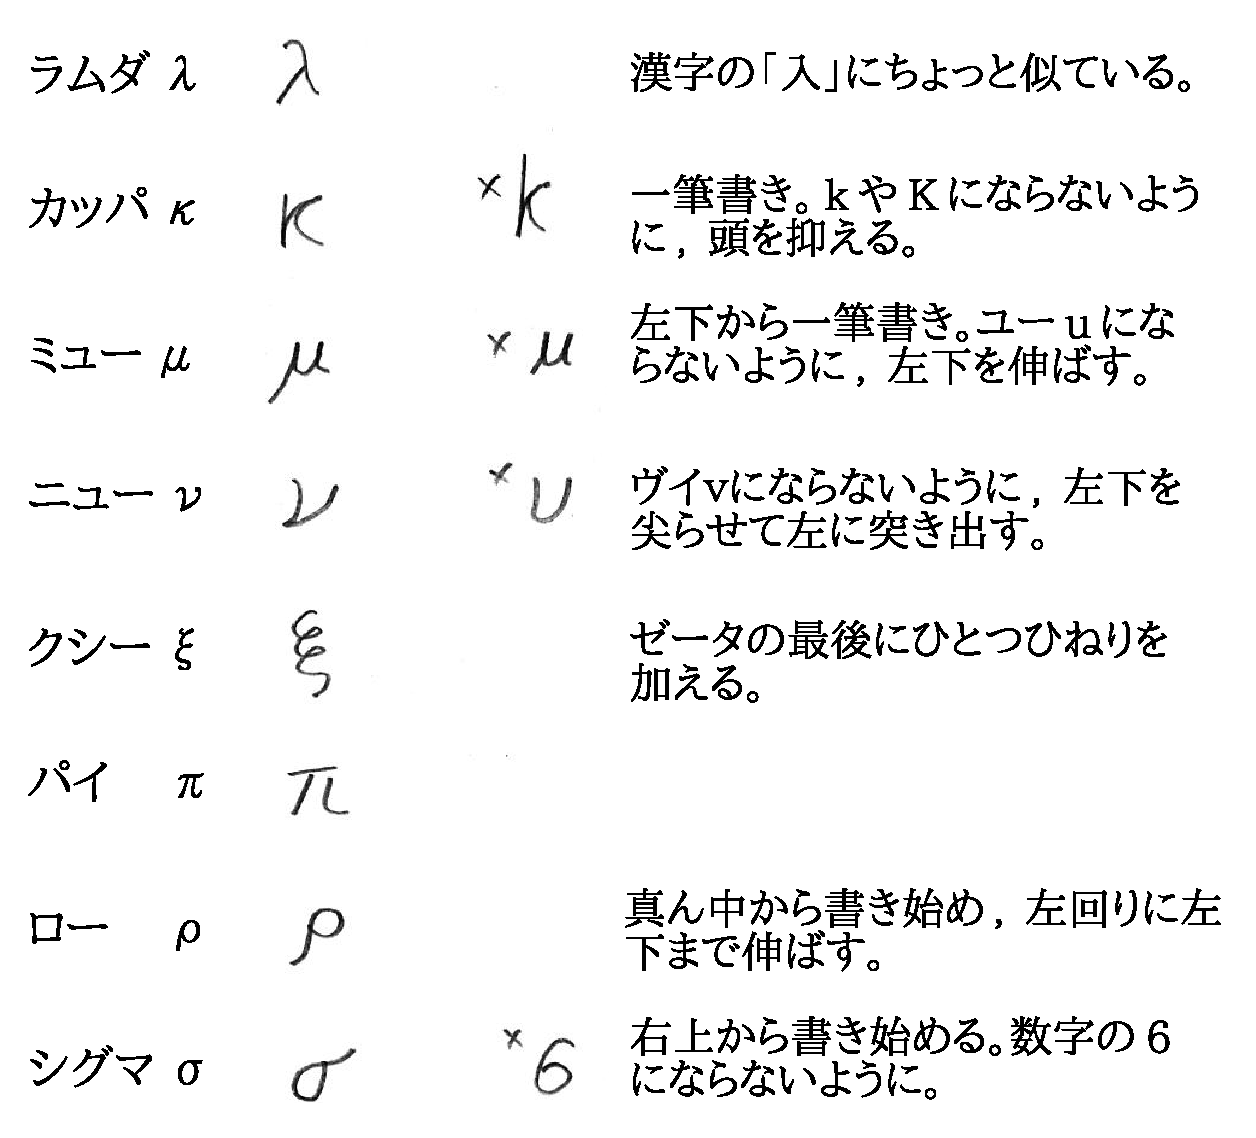
\includegraphics[width=7.5cm]{Greece2.eps}
    \caption{ギリシア文字の小文字($\lambda, \kappa, \mu, \nu, \xi, \pi, \rho, \sigma$)の書き方。$\times$がついているのは, よくある間違った書き方。\label{fig:Greece2}}
\end{figure}

\begin{figure}[H]
    \centering
    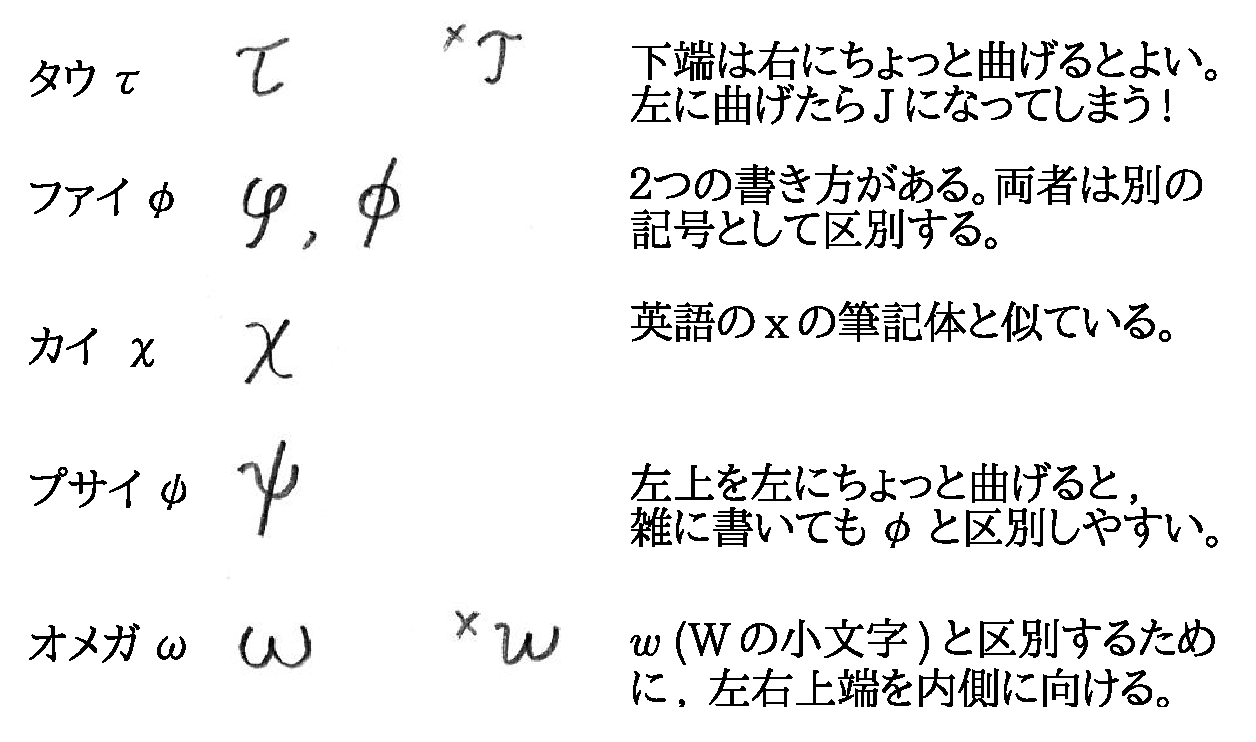
\includegraphics[width=7.5cm]{Greece3.eps}
    \caption{ギリシア文字の小文字($\tau, \phi, \chi, \psi, \omega$)の書き方。$\times$がついているのは, よくある間違った書き方。\label{fig:Greece3}}
\end{figure}

\begin{figure}[H]
    \centering
    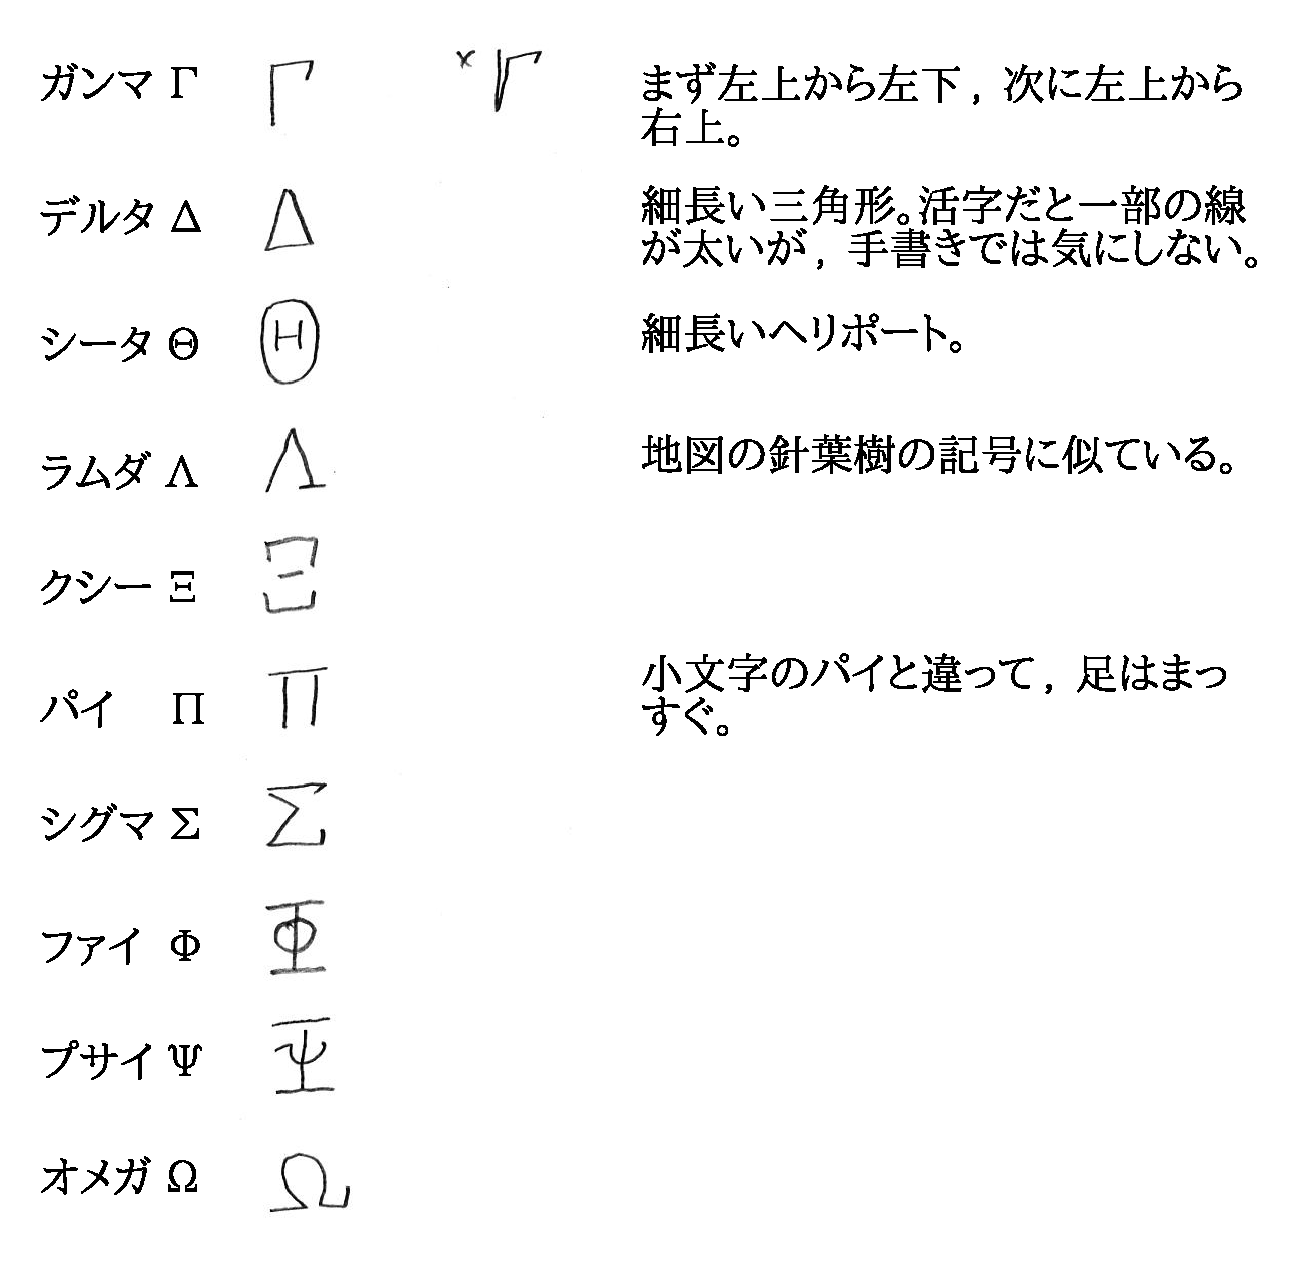
\includegraphics[width=7.5cm]{Greece4.eps}
    \caption{ギリシア文字の大文字($\Gamma, \Delta, \Theta, \Lambda, \Xi, \Pi, \Sigma, \Phi, \Psi, \Omega$)の書き方。$\times$がついているのは, よくある間違った書き方。\label{fig:Greece4}}
\end{figure}

\begin{freqmiss}{\small\textgt{以下の文字の書き分けができない: \\$\gamma$と$r$, $\delta$と$8$, 
$\eta$と$n$, $\kappa$と$k$, $\mu$と$u$, $\nu$と$v$, 
$\sigma$と$6$, $\chi$と$x$, $\omega$と$w$。}}\end{freqmiss}

\begin{faq}{\small\textgt{高校まで三角形を「$\triangle$」とかいていたのですが, 
デルタ「$\Delta$」と三角形「$\triangle$」は書き分けがあるのですか?}
... 手で書くときは, $\Delta$はちょっと細長く, しかも右に傾いた感じで書きます。
ちなみに$\triangle$は大学では「ラプラシアン」という概念を意味する記号でもあります。}\end{faq}

\begin{faq}{\small\textgt{$\Omega$って「オーム」じゃないんですか?}
... 中学校理科で習った電気抵抗の単位$\Omega$。これを「オーム」と呼ぶのは, 
「オームの法則」というのを発見したOhmさんという物理学者の名に由来します。
電流の単位をAと書いて「アンペア」と呼ぶのと同じようなものです
(アンペアはAmpereという物理学者の名に由来)。Ohmさんの頭文字だから, 
大文字のOにしたかったのでしょうけど, 数字の零と紛らわしいので, 
Oに対応するギリシア文字の$\Omega$を採用した, というわけです(多分)。}\end{faq}

\begin{faq}{\small\textgt{携帯電話の記号のところにギリシャ文字が入っているのですが, 
$\iota$や$o$とは何ですか?}
... それぞれイオタ, オミクロンといいます。数学ではあまり使いません。}\end{faq}

\begin{faq}{\small\textgt{$\xi$とか$\eta$とかって, これまで実際に見たこと
はありません。本当に使うのですか? }
... 大学で専門的な勉強をしていくと, いろんなところで出てきますよ。}\end{faq}
\mv


\section*{演習問題}

%\begin{exq}\label{q:unit_missing} 無限大$\infty$を数(実数)の
%ひとつとして認めてしまうと, どういう困ったことが生じるか, 四則演算の公理に
%基いて述べよ。\end{exq}

\begin{exq} 任意の自然数$x$について, $x$を10進法で表したとき, 
各桁の数(0以上9以下)を全部足したものが3で割り切れれば, $x$は3で
割り切れる。これを証明せよ。\end{exq}

\begin{exq}\label{q:div_by_zero} もし「0で割る」ことができるなら, どのような矛盾が生じるか?\end{exq}
%\noindent{\textbf{答}}\ref{q:div_by_zero} 
% もし$2\div 0$が可能ならば, その答を$x$とすれば, 
%$2\div 0=x$である。すると, 割り算の定義から, $2=0\times x=0$
%となり, $2=0$という, 変な等式が出てきてしまう。\\

\begin{exq}\label{q:base_zero} \eref{eq:taisuu00}のすぐ後に
「ただし$a\neq1$とする」という条件があった。もし$a=1$を考えると, 
どのような困ったことが起きるか?\end{exq}

%\答 $a=1$のとき, すなわち$\log_1 x$は, 「1を何乗したら$x$になるか?」である。
%ところが, 1は何乗しても1だから, $x=1$のときを除いて, $\log_1 x$は存在しないので, $\log_1 x$を考えるのはほとんど無意味である。\\

\begin{exq}\label{q:triangle_gravxenter} 三角形ABCの各頂点に, 
互いに等しい質量のおもりがくっついている。辺BCの中点をDとすると, 
この3つのおもりの重心は, 線分ADを2:1に内分する点にあることを, 
位置ベクトルを使って示せ。ヒント: A, B, Cの各位置ベクトルを${\bf a}$, 
${\bf b}$, ${\bf c}$とすると, 3つのおもりの重心の位置ベクトル${\bf r}$は, 
${\bf r}=({\bf a}+{\bf b}+{\bf c})/3$である(これは重心の定義)。
\end{exq}

%\begin{exq}\label{q:alg_def_speed} 速さの定義を述べよ, という問に, 
%C君は「進んだ距離(m)をかかった時間(秒)で割ったものを速さという」と答えた。
%これは定義として適切か?
%\end{exq}
%\noindent{\textbf{答}}\ref{q:alg_def_speed} 
%不適切。mや秒という単位まで指定するのは蛇足である。m以外の単位で距離を測り, 
%秒以外の単位で時間を測って割り算をしたものも「速さ」である。\\
\hv


\section*{問の解答}
{\small ここに解答が出ていない問題は, 解答が省略されている。各自, 自力で解こう。
また, 「略解」では最終的な答だけが述べられいるが, 君はきちんと導出過程も書くこと。\mv}

\noindent{\textbf{答}}\ref{q:badhabit_equality} 
ここでは「A君は学生である」の「は」を等号とみなしたのが間違い。
学生にはA君以外の人もいるし, A君は学生以外の属性(男性とか, 
茨城県出身とか, ...)も持つので, 「A君」と「学生」は同じではない。\mv

%\noindent{\textbf{答}}\ref{q:alg_num0} 自然数とは, 1を繰り返し足してできる数。整数とは, 自然数から自然数をひいてできる数。有理数とは, 整数を(0以外の)整数で割ってできる数。\mv

%\noindent{\textbf{答}}\ref{q:alg_def_pi} 「3.1415926, 以下, ずっと値が続く数」には, 3.1415926111...や, 3.1415926222...など, いろんな数があるので, この発言では円周率を特定できない。\mv

%\noindent{\textbf{答}}\ref{q:axiom_shisokuenzan} 略(がんばれ!)

%\noindent{\textbf{答}}\ref{q:th_zero} 略(本文の該当箇所をまとめればOK)

\noindent{\textbf{答}}\ref{q:bad_notation0} (1) $a$が分母なのか分子なのか
わからない。(2) $3\times(-4)$と書くべき。(3) 二重括弧は外側を\{\}に。また, 末尾の$x$が
分母なのか分子なのかわからない。

%\noindent{\textbf{答}}\ref{q:alg_order2}
%\begin{enumerate}
%\item \eref{eq:axiom_order2}で, $c=-a$とすれば, $a-a<b-a$。
%この左辺は, \eref{eq:axiom_num_sum_inv}より0。従って$0<b-a$。
%\item $a<b$のとき, 前小問より$0<b-a$。\eref{eq:axiom_order3}で
%$a$を$c$に, $b$を$b-a$に置き換えれば, $0<c(b-a)$。
%この右辺は, \eref{eq:axiom_num_distr}で$a$を$c$に, $b$は$b$のままに, 
%$c$を$-a$に置き換えれば, $cb-ca$となる(以下, このような置き換えに
%ついての記述は省略する)。従って, $0<cb-ca$。両辺に
%$ca$を足せば, \eref{eq:axiom_order2}より$ca<cb$。\eref{eq:axiom_num_mult_exch}
%を両辺に適用して, $ac<bc$。
%\item $c<0$の両辺に$-c$を足すと(\eref{eq:axiom_order2}より)$0<-c$となる。
%前小問の$c$を$-c$に置き換えれば, $a(-c)<b(-c)$。従って, $-ac<-bc$。この
%両辺に$ac+bc$を足せば, $-ac+(ac+bc)<-bc+(ac+bc)$。\eref{eq:axiom_num_sum_assoc}を
%左辺に使えば, 左辺=$(-ac+ac)+bc=bc$。\eref{eq:axiom_num_sum_exch}を右辺に使い, 
%続けて\eref{eq:axiom_num_sum_assoc}を使えば, 右辺=$(ac+bc)-bc=ac+(bc-bc)=ac$。
%従って, $bc<ac$。
%\end{enumerate}

%\noindent{\textbf{答}}\ref{q:alg_ineq3} 略。
%$|a^2|=|a|^2=a^2,\, |a||b|=|ab|$等に注意。
%\begin{enumerate}
%\item 略(左辺を展開)
%\item $0\leq a+b$のとき, \eref{eq:alg_abs1}の$a$を$a+b$で置き換えて考えれば, $|a+b|=a+b$である。
%従って, $|a+b|^2=(a+b)^2=a^2+2ab+b^2$。\\
%$a+b<0$のとき, \eref{eq:alg_abs2}の$a$を$a+b$で置き換えて考えれば, $|a+b|=-(a+b)$である。
%従って, $|a+b|^2=\{-(a+b)%\}^2=(a+b)^2=a^2+2ab+b^2$。
%\item (1)$-$(2)より明らか。
%\item $|ab|$は$ab$と等しいか($ab \ge0$のとき), $ab$より大きい($ab<0$のとき)。
%従って, $ab \le |ab|$。よって$0 \le |ab|-ab$。
%\item (3)(4)より, 明らか。
%\item 絶対値か, 絶対値の足し算だから, 0以上なのは自明。
%\item (6)と命題8より, (5)の両辺の平方根をとっても不等号の向きはかわらない。
%\end{enumerate}
\mv

\noindent{\textbf{答}}\ref{q:alg_pow0} (1) 32 (2) $1/2^2= 1/4$ (3) $10^{-2} = 1/100$
(4) $9^{1/2} = \sqrt{9} = 3$ (5) 1 (6) $10^4$\mv

\noindent{\textbf{答}}\ref{q:alg_pow1} (1) $\,\,\,3^{-1/2}\,\,\,\,\,\,\,\,$ (2) $\,\,\,5^{1/3}$
\mv

\begin{comment}
\noindent{\textbf{答}}\ref{q:sqrt_ab} 
\begin{enumerate}
\item 
$(\sqrt{a}\,\sqrt{b})^2=\sqrt{a}\,\sqrt{b}\,\sqrt{a}\,\sqrt{b}
=\sqrt{a}\,\sqrt{a}\,\sqrt{b}\,\sqrt{b}=(\sqrt{a})^2\,(\sqrt{b})^2=ab$。
また, $\sqrt{a}\geq0$, $\sqrt{b}\geq0$は自明だから, $\sqrt{a}\,\sqrt{b}\geq0$。
すなわち$\sqrt{a}\,\sqrt{b}$は$ab$の0以上の平方根。すなわち, 
$\sqrt{a}\,\sqrt{b}=\sqrt{ab}$。\qed
%ちなみに, この考え方を発展させれば, 任意の実数$\alpha$について, 
%$(ab)^\alpha=a^\alpha b^\alpha$が証明できる。
\item $\sqrt{10}=\sqrt{2\cdot5}=\sqrt{2}\sqrt{5}=1.414\cdots\times2.236\cdots=3.162\cdots\fallingdotseq3.16$。
これは, $\pi=3.1415\cdots$より大きい。注: $\sqrt{10}$が$\pi$に非常に近い数であるということは, 
豆知識として知っておいて損はない。
\end{enumerate}
\end{comment}

\noindent{\textbf{答}}\ref{q:alg_dentaku2} (?は秘密!) (1) 11.313?? (2) 2.704?? (3) 1.709??\mv

%\noindent{\textbf{答}}\ref{q:Napier_value_memorize} 略。(がんばれ!)\mv

\noindent{\textbf{答}}\ref{q:alg_dentaku_exp} 略解として小数第3位までで打ち切った値を示す。
レポートでは小数5位まで書くこと。\\(1) 7.389 (2) 0.223\mv

\noindent{\textbf{答}}\ref{q:exp_logvalue0} (1) $2$ (2) $4$ (3) $2$ (4) $3$ (5) $-2$ (6) $0$\mv

%\noindent{\textbf{答}}\ref{q:whatis_log} 略。\mv

\noindent{\textbf{答}}\ref{q:alg_dentaku_ln} 
略解として小数第3位までで打ち切った値を示す。
レポートでは小数5位まで書くこと。(1) 0.301 (2) $-2.221$ (3) 0.693 (4) 2.302\mv

%\noindent{\textbf{答}}\ref{q:vect_write} 略。(がんばれ!)\mv

\noindent{\textbf{答}}\ref{q:vect_add_fig} 略。図の上に作図してみよ。
ベクトルはどこに置くかを問題としないことに注意!
\mv

% 点A(4, 5)と点B(3, 6)について,
\noindent{\textbf{答}}\ref{q:vect_pos2D}  点A, Bの位置ベクトルをそれぞれ${\bf a}$, ${\bf b}$とすると
\begin{eqnarray*}\text(1)\quad\frac{2{\bf a}+{\bf b}}{3}=\Bigl(\frac{11}{3}, \frac{16}{3}\Bigr)\quad\quad
                 \text(2)\quad\frac{{\bf a}+2{\bf b}}{3}=\Bigl(\frac{10}{3}, \frac{17}{3}\Bigr)\end{eqnarray*}

\noindent{\textbf{答}}\ref{q:guard_digit_order} 
(1) 5, 3の2桁。 (2) 1, 2, 3, 0, 5の5桁。 (3) 5, 3は確実に有効数字だが, 
そのあとの2つの0は有効数字かどうかわからない。 (4) 2, 3, 0の3桁。\mv

\noindent{\textbf{答}}\ref{q:guard_digit_prac2} (1) 11.9 (2) 123.5 (3) 87\mv

\noindent{\textbf{答}}\ref{q:guard_digit_prac4} (1) 14 (2) 2.8 (3) 7.7\mv

\noindent{\textbf{答}}\ref{q:guard_digit_8} (1) 12.8 cm (2) 13 cm 
(3) 略(君の考えを正直に述べよ)\mv

\noindent{\textbf{答}}\ref{q:guard_digit_9} 
(1) 13.1から13.3までなので, 0.1の桁が不確定と見て, 13.2。 (2) 13.0から13.4までなので, 
これも0.1の桁が不確定と見て, 13.2。 (3) 12.6から13.8までなので, 1の桁が不確定とみて, 
13。

%\noindent{\textbf{答}}\ref{q:logic_Greece} 略。(がんばれ!)


%\begin{faq}{\small\textgt{演習問題の答が欲しいです} ... 考えることを楽しんで欲しいので, あえて載せていません。どうしても知りたければ質問においで。一緒に考えよう!}\end{faq}

%\begin{faq}{\small\textgt{勉強すれば本当に数学が好きになりますか? リメディアル教材の内容を出来るようになる自信がありません} ... 「はじめに」に載っている勉強法を守って丁寧にやれば大丈夫。そうすると, だんだん楽しくなって, 数学が好きになってきます。やみくもに焦ってストイックに頑張るだけでは, すぐに心折れちゃって, 数学が嫌いになっちゃうよ。}\end{faq}

%\begin{faq}\small{\textgt{大学で高校数学の復習なんて, ゆるくないですか?}... ゆるくないです。高校数学の復習は, 全ての大学生に必要です。高校数学は, 大学入試の問題演習が中心ですので, 「問題は解けるけど, 基礎を理解していない」という人が多いのです。そんな状態のままで大学数学を詰め込まれ, 消化不良を起こして脱落する大学生がたくさんいます。}\end{faq}



\include{01_num_ans}
\chapter{物理量と単位}\label{chapt:dim_unit}
%{\small 君は「はじめに」を全部, 隅々まで読みましたか? 
%読まずに進むと, 誤った方法で勉強することになり, 時間と努力を無駄にします。}\\

\section{物理量は, 数値×単位}\label{sect:dimension}

数学は数を抽象的な概念として扱う。例えば数学で
「方程式$3x=x+4$の解は$x=2$である」
という時の$x=2$は, 何か具体的なものの量を想定してはいない。

一方, 現実の様々な問題では, 何らかの実体を伴った具体的な量
を扱う。例えば「君の身長」や「君の100~m走の記録」は
具体的な実体を表す量である。このように, 具体的な実体を
表す量のことを\underline{物理量}\index{ぶつりりょう@物理量}
と呼ぶ\footnote{物理が嫌い!苦手!という人もいるが, 
世の中の量のほぼ全ては「物理」量であり, その計測や扱い
において, 物理学の考え方は必要である。}。

物理量は, 通常, 160 cmとか12.3 秒というふうに, 数値と単位の
積(掛け算)で表される。君は160 cmというとき, 
cmという単位は, 160という数値のオマケか添え物のように
思っているかもしれないが, そうではない。160 cmとは
\begin{eqnarray}
160 \times\text{ cm}
\end{eqnarray}
という意味だ(積を表す$\times$は省略されている)。
つまり, 160 cmは, 「cm(センチメートル)を160個
ぶん集めた量(長さ)」だ。同様に, 12.3秒とは
$12.3\times$秒であり, 「秒を12.3個ぶん集めた量(時間)」
だ。このように, 物理量の大きさは
「何の何個分」という形で表され, その「何の」に相当する
のが\underline{単位} (unit)\index{たんい@単位}である
\footnote{「単位」は多義語であり, 大学の授業をいくつ
履修したか(英語では"credit")を表する時も使う。}。

物理量の扱いで, 数値が正しくても単位を間違えると大惨事になる。

\begin{exmpl} 1999年9月23日, 米国の火星探査機
「マーズ・クライメート・オービター」が, 火星に到達した
直後に, 消息を断った。探査機を制御する2つのチームが, 
片方はメートルやキログラムという単位を使い, もう片方は
ヤードやポンドという単位を使っており, データ共有に失敗して, 
制御不能で事故に至ったらしい。\end{exmpl}

\begin{exmpl} 2000年3月30日, 埼玉県川口市の病院で, 
ある患者が, 薬剤を過剰投与され, 死亡した。
医師の指示では薬剤は80 mgだったが, 処方箋には, 
80アンプルと記入され(1本のアンプルには10 mgの薬剤が入っている), 
結果的に, 看護師が800 mgの薬剤を投与したらしい。(例おわり)\end{exmpl}

しかし, 大変残念ながら, 伝統的に, 生物資源学類生の多くは, 
単位が苦手であり, 単位を平気で付け忘れる\footnote{その一部は, 
単位に自信がないから, 「つけ忘れたふり」をしてごまかしてるのだろう。}。
当然, そのような答案は不正解であり, 0点である。いにしえの資源生曰く, 
「\textgt{単位(unit)を忘れて単位(credit)を落とす}」と。

\begin{faq}{\small\textgt{そこまで単位にこだわらなくても
いいのでは?} ... 
君が農家で, 単位を間違えて基準を超える濃度で農薬撒いたら
どうなります? 野菜全部出荷停止ですよ。}

%\begin{faq}{\small\textgt{そういうシリアスな状況では, 
%もちろんちゃんと単位つけますよ。} ...
%そんなこという人の野菜なんか, 怖くて誰も買いませんよ。
%大切なことは, 普段から気をつけて習慣にしておかないと, 
%いざというときにミスするのです。}\end{faq}

{\small\textgt{でも, 高校や, 大学でも他の授業では, 
単位の付け忘れは減点だけです。0点なんて, 厳しすぎませんか?}
... そんなぬるい教育をするから大惨事が起きるのです。}

{\small\textgt{でも, 「三角形ABについて
辺ABの長さを$1$とする」みたいに, 最初から単位が無い
問題文もあるじゃないですか? }
... 数学でよくあるそういう問題は, 
ABの長さが1~cmであっても, 1~mであっても, 1~kmであっても
通用するように作られているのです。こういうときは
答にはもちろん単位をつける必要は無いし, つけてはダメ。}

{\small\textgt{物理でも, 「力を
$F$とし, 質量を$m$とする...」みたいに, 単位が書かれて
いない問題がありますよね?} ... 単位はその$F$や$m$の
\textgt{中に}含まれているのです。例えば$m$を実際に
数値で表すと, 「$m=3$~kg」や「$m=3000$~g」
と書いたりします。このとき, $m$には, 3や3000という数値
だけでなくkgやgという\textgt{単位も一緒に入っている}のです。}

{\small\textgt{「$t$秒の時間で, 
毎秒2~mの速さで, 6 m進んだ。$t$を求めよ」みたいな問題は? 
「$t=$3 秒」ですか?「$t=$3」ですか?} ... 問題文で, 
その時間は「$t$かける秒」で定義されている(単位は
変数$t$の外に出されている)ので, $t$は単位を持って
いません(後述する無次元量)。従って$t=3$が正しいです。
でもこういう書き方は稚拙であり, 大学では一般的ではありません。
}\end{faq}

さて, 複数の物理量どうしを足したり引いたり, 大小を比べたりするには, 
単位を揃える必要がある。例えば, 「20 cm + 1.23 m=?」という問は, 
\begin{eqnarray}
&&0.2\text{ m} + 1.23\text{ m} = 1.43\text{ m}\label{eq:0.2m+1.23m}\\
&&20\text{ cm} + 123\text{ cm} = 143\text{ cm}\label{eq:20cm+123cm}
\end{eqnarray}
というふうに, ひとつの単位に揃えないと計算できない。また, 
20 cmと1.23 mのどちらが大きいか? という問に, 20と1.23という
数の大小だけで判断して「20の方が大きい!」というのは愚かである。

こういう話をアタリマエだ! と思わずに, よく考えよう。
\eref{eq:0.2m+1.23m}を丁寧に考えれば, まず左辺の2つの
項をmという量でくくって, 左辺=(0.2 + 1.23) m
という式を立て, その括弧内を普通に数どうしの足し算で計算し, 
右辺の1.43 mに至るのだ。この「共通する量でくくる」ところで, 
暗黙のうちに分配法則(\eref{eq:axiom_num_distr})を逆向きに
使っているのだ! それは, 0.2~mや1.23~mという量を, ともに
「同じ単位の何倍か」に揃えたからできたのだ。改めて, 
単位は単なる添え物ではなく, 物理量の重要な一部だと感じられ
るではないか!\mv

\section{次元}

さて, どんなに頑張っても単位を揃えられないような量どうしも
存在する。例えば20 cmと5 時間がそうである。前者は長さ, 
後者は時間を表すのだから, 単位は揃えられない。

こう考えれば, 世の中の様々な物理量は「互いに単位を
揃えられるかどうか」という観点で分類できるだろう。
そういう性質を「\underline{次元}」\index{じげん@次元}
と呼ぶ。上の例では, 20 cmという量は「長さ」という次元を持ち, 
5 時間という量は「時間」という次元を持つ。\mv

\begin{q}\label{q:alg_dim00} (本節で出てきた)次元とは何か?\end{q}

次元が違う量どうしは, 足したり引いたり, 大小を比較したり
はできない。実際, 20 cmと5 時間を「足す」ことはできないし, 
無理に20と5を足して25を得ても, それはもはや何の物理量も
表さない。「20 cmと5 時間はどちらが大きいか」などという
問も無意味である。\\



\section{単位の掛け算と割り算}\label{sect:unit_mult_div}

ところで, 単位は, 普通の数と同じように掛け算ができる:

\begin{exmpl} 隣接する2辺の長さが2 mと3 mで
あるような長方形の面積は, 
\begin{eqnarray}
2\text{ m}\times3\text{ m}=6\text{  m}^2\label{eq:rect_area00}
\end{eqnarray}
である。このとき, 結果にm$^2$という単位が出てきたのは, 
「面積を求めたから」というよりも, 「mを2回掛けたから」
なのだ。(例おわり)\end{exmpl}

単位は, 割り算もできる:

\begin{exmpl} 100 mの距離を20 秒で走る人の(平均の)速さは, 
\begin{eqnarray}
\frac{100\text{ m}}{20\text{ 秒}}=5 \text{ m}/\text{ 秒}\label{eq:100m20s_speed}
\end{eqnarray}
となる。このとき, 単位どうしの割り算の結果として, 
速さの単位「m/秒」が出てきた。\textgt{この単位の/という
記号は, 割り算の記号}なのだ。従って, m/秒を$\frac{\text{m}}{\text{秒}}$
と書いてもOKである。(例おわり)\end{exmpl}

\begin{faq}{\small\textgt{割算に/という記号をなるべく使わない, 
という約束がありましたが, m/秒はOKなのですか?} ... 
慣習的に, 単位の中では/をよく使います。例外ということに
しておきましょう(国際規格でも認められている)。}\end{faq}

「5~m/秒」は「5メートル毎秒」とか「毎秒5メートル」とも言われる。
このような「毎...」は, 「...という単位あたり」と同じ事である。
「5メートル毎秒」は「1秒あたり5 m」と同じである。
そして, 「...あたり」は「...で割る」という意味である。たとえば, 
「りんご6個を3人でわけるとき, 一人\textgt{あたり}いくつ?」
という問には, 6個$\div$(3人)で計算するだろう。

困ったことに, 世の中にはこの「毎...」や「...あたり」を省略するという
悪習がある。決して真似てはいけない。

\begin{exmpl} 日本のGDP(国内総生産)は, 1人あたり約4万ドルと
言われることがある。これは, 1人あたり\underline{1年間あたり}
約4万ドル, もしくは約4万ドル/(人・年)が正しい。\end{exmpl}

\begin{exmpl} テレビの天気予報では, 「台風の中心付近の
最大瞬間風速は40~m」などと言われるが, これは\underline{毎秒}40~m, 
もしくは40~m/秒が正しい。\end{exmpl}

\begin{exmpl} 放射線量を表すときに使われるSv (シーベルト)
とSv/h (シーベルト毎時)は全く違う単位なのに, 
後者を省略して前者のように言ってしまう報道が多い。
これはヤバイ。例えば1~$\mu$Sv/hと1~$\mu$Sv/sは, 
/hや/sを省略したら同じ表現になってしまうが, 実際は, 
後者は前者の3600倍である。(例おわり)\end{exmpl}\mv

こういう悪習を人前で晒すと恥をかく。その恥は, 本人だけ
でなく, 出身大学まで及ぶ。

ここまで読んで, 君は「面倒くさ!」と思ってる
かもしれないが, 単位は君を助けてくれることもある。
次節では小学校レベルの問題を扱うが, 意外に苦手な人も多い。
そういう問題で, 単位が役に立つのだ。\\

\section{単位を埋め込んで計算せよ!}
ところで, \eref{eq:rect_area00}を, 次のように書く人が多い:
\begin{eqnarray}
2\times3=6\text{  m}^2\label{eq:rect_area00_NG}
\end{eqnarray}
高校の参考書もこういう記法を勧めてたり, 大学教員にもこう書く
人がいるが, これは変だ。なぜか? もしこういう書き方がOKなら, 
「2辺の長さが2~cmと3~cmの長方形の面積は?」という問題についても, 
\begin{eqnarray}
2\times3=6\text{  cm}^2\label{eq:rect_area00_NG2}
\end{eqnarray}
と書けるはずだ。\eref{eq:rect_area00_NG}と\eref{eq:rect_area00_NG2}の
左辺は共通なので, 等号の公理(\eref{eq:equality03})から, 
\begin{eqnarray}
6\text{  m}^2=6\text{  cm}^2\label{eq:rect_area00_NG3}
\end{eqnarray}
\textgt{これは明らかに変だ!} その原因は, 
\eref{eq:rect_area00_NG}と\eref{eq:rect_area00_NG2}の
左辺に単位を埋めこまなかったことにある。\textgt{単位を持つ量
の計算は, 式の中に数値だけでなく単位も埋め込む}べきなのだ。
そうすれば, 単位の誤記や, 単位のつけ忘れという重大なミスを
防止できる。\mv

式の中に単位を埋め込みたくなければ, \eref{eq:rect_area00_NG}
や\eref{eq:rect_area00_NG2}の右辺の単位も書かなければよい。
それは, 単位を外した数値\footnote{それは後述する「無次元量」である。}
の間の計算であり, 論理的には問題ない。そして出てきた数値に改めて
単位をつけた答を, 別の場所に書くのだ。それもめんどくさい人は, 
\begin{eqnarray}
2\times3=6\quad\quad\text{[m$^2$]}\label{eq:rect_area00_NG5}
\end{eqnarray}
と書いたりする。この場合, 右の方の[m$^2$]は, 「最後に出てきた数値に
この単位を掛けたものが, 最終的な答えですよ」という事情を書き添えた
「メモ」であり, 等式の一部ではない。

しかし\textgt{これらはいずれも不合理な慣習である}。やはり単位を埋め込んで
計算すべきなのだ。そうすれば, \textgt{単位が計算を助けてくれる}ことがあるのだ。\mv

\begin{exmpl}\label{exmpl:niku600yen} 120~gで600円の肉は, 900~gでいくらか? 
もちろん, 「120~gあたり600円」だから1 gあたり... と考えて, 
ここは割り算, ここは掛け算, というふうに進めてもいいが, 
単位を頼りに考えると楽なのだ:
\begin{eqnarray}
\frac{600\text{円}}{120\text{ g}}\times 900\text{ g}=
\frac{600\times900}{120}\frac{\text{円}\teisei{\text{ g}}}{\teisei{\text{ g}}}
=4500\text{ 円}\quad\quad\quad\label{eq:mihaji02}
\end{eqnarray}
\eref{eq:mihaji02}の左辺には, それぞれの数値に単位をつけた。
つまり, 単位を式に埋め込んだ。数値と単位は掛け算の関係なので, 
順番を入れ替えて, 数値の計算と, 単位の計算に分離する。
そして数値は数値で計算し, 単位は約分して簡単にする。
そうすれば, 最後に「円」という欲しかった量の単位が現れ, 
立式が正しかったことが裏付けられる。
もしもこの問題を, うっかり
\begin{eqnarray}
\frac{120\text{ g}}{600\text{円}}\times 900\text{ g}=...\label{eq:mihaji04}
\end{eqnarray}
とやっちゃったら, 最終的な単位がg$^2$/円になる。
これは意味不明なので, 何か間違っていた, とわかるのだ。\end{exmpl}

\begin{exmpl}\label{exmpl:mihaji} 小学校で, 速さと道のりと時間の関係を, \\
 「速さ=道のり$\div$時間」\\
 「道のり=速さ$\times$時間」\\
 「時間=道のり$\div$速さ」\\
と習った。これを, いわゆる「みはじ」, つまり
\begin{eqnarray}
\frac{\text{み}}{\text{は }|\text{ じ}}
\end{eqnarray}
という図式(「み」は道のり, 「は」は速さ, 「じ」は時間)で
覚えた人も多いだろう(「みはじ」以外にも「きはじ」とか
「はじき」とか「木の下にはげ爺さん」などのバージョンもあるらしい)。
しかし, このような図式を忘れても, 単位をチェックすれば
正しく計算できる。実際, 速さをm/秒, 道のりをm, 時間を秒
で表すならば, 例えば速さ3~m/秒で時間5秒だけ走るときの道のりは, 
単位も埋め込んで正しく計算すれば\\
\begin{eqnarray}
3\frac{\text{m}}{\teisei{\text{秒}}}\times 5\teisei{\text{秒}} = 15\text{ m}\label{eq:mihaji06}
\end{eqnarray}
となり, 無事に距離の単位mが出てくる。ところが, これを
割り算にしたりすると, m/秒$^2$や秒$^2$/mという, 変な単位
が出てくる。そういう変な単位にならないように, すなわち, 
目標とする単位が最終的に残るように立式すればよいのだ。(例おわり)\end{exmpl}

「速さ, 道のり, 時間」のように, 互いに積や商の関係
にあるような3つの量を処理するという状況は, 他にも
たくさんある。それらのひとつひとつに
「みはじ」みたいなのを考えるのはきりがない。
単位を埋め込んで, 単位を手がかりに処理すればいいのだ。
\mv

\begin{faq}{\small\textgt{でも, このやりかた, めんどくさいです。} ... 
私も最初はそうでした。でも, 結局はこの方が正確で便利なのです。
数値だけの計算だと, ミスしやすいのです。ミスの発見と修正には
多くの時間が必要ですからね。それに, 学校のテストならミスは
減点だけですが, 仕事でのミスは大事故や大損害になりかねません。}\end{faq}
\mv

\begin{q}\label{q:unit_mihaji} 以下の問を, 単位を式の中に埋め込んで解け。
\begin{enumerate}
\item 5時間で500リットルの水が出る蛇口から2時間で流れ出る水の量を求めよ。
\item 5時間で500リットルの水が出る蛇口から4~m$^3$の水を出すのに,どのくらいの時間がかかるか?
\item つくば市の水田面積は約4900~ha, コメの収穫は年間21,000~tである(つくば市ホームページ)。つくば市の水田は1年間で, 
単位面積あたり, どのくらいのコメがとれるか? kg/m$^2$という単位で答えよ。
\item つくば市で, 単位質量のコメの生産に必要な水田の面積を求め, m$^2$/kgという単位で答えよ。
\item 筑波大学の筑波キャンパスは, 約260万m$^2$である。これと同じ面積の水田をつくば市で借りたら, 
年間何トンのコメがとれるか?
\item 日本の成人1人は年間約60~kgのコメを消費する。生物資源学類1年生約130人の消費するコメを
つくば市の水田だけでまかなうなら, どのくらいの面積の水田が必要か?
\item タイのある農村に, 面積120~haのキャッサバ農地がある。ここで毎年収穫されるキャッサバの総額は日本円で概ねいくらか? ただし, 当地方のキャッサバ農地では毎年, キャッサバは1ライあたり平均約2.5トン収穫されることが別の調査でわかっている。ライというのはタイで使われる面積の単位で, 1ライは1600~m$^2$である。また, キャッサバの市場価格は4.4バーツ/kgである。バーツというのはタイの通貨単位で, 100円が33バーツである。
\end{enumerate}
\end{q}



\section{無次元量}

ところで, 同じ次元を持つ量どうしの割り算は, 面白い結果になる。
例えば, 直径$d$の円の周長を$S$とすると, $d$も$S$も次元は
「長さ」であり, 数値と単位(cmやmなど)の積で表現される。
ところが$d$と$S$をひとつの単位に揃えた上で$S/d$という量を
計算すると, 長さの単位は約分されて消え, $3.141592...$という
数だけが残る(これは円の大きさがどうであれ一定値であり, それが
円周率$\pi$である)。この量には単位が無い! このように, 
単位を伴わずに数だけで表現できる量を\underline{無次元量}
\index{むじげんりょう@無次元量}
とか\underline{無名数}\index{むめいすう@無名数}という。

物理量を数と単位の積で表すとき, その数は無次元量である。例えば, 
ある長さ$L$が, $L=15$~cmであるとする。この両辺をcmという量(1~cm)で割ると, 
\begin{eqnarray}
L/\text{cm} = 15\label{eq:L/cm=15}
\end{eqnarray}
となる。左辺は, $L$もcmも長さという次元の量であり, 従って, 
その割り算は無次元量になる。従って, 右辺の15は無次元量である。

\eref{eq:L/cm=15}は見慣れない, 奇妙な印象を受ける
式かもしれない。しかしこれは国際的にも認められた, 立派な
表記法である。特に, 科学的な論文の表やグラフの中で, このような表記が
しばしば用いられる。\\


\section{SI単位系}

いろんな単位を無秩序に併用すると混乱する。そこで, それぞれの次元に対応
する単位をひとつずつ定めて, 統一的に使うと便利だ。そのように定めた
単位のセットのことを\underline{単位系}\index{たんいけい@単位系}と呼ぶ。
科学の世界では, 一般的に, \underline{SI単位系} (国際単位系ともいう)
\index{SIたんいけい@SI単位系}と呼ばれる, 国際的に合意決定された
単位系を\textgt{優先的に}使う。

SI単位系は, まず, 以下の7つの単位が骨格である:
\begin{itemize}
\item 長さの単位: m (メートル)
\item 質量の単位: kg (キログラム)
\item 時間の単位: s (秒)
\item 電流の単位: A (アンペア)
\item 温度の単位: K (ケルビン)
\item 物質量 (個数) の単位: mol (モル)
\item 光量 の単位: cd (カンデラ)
\end{itemize}
↑これらの7つの単位を\underline{SI基本単位}\index{SIきほんたんい@SI基本単位}と呼ぶ。
SI基本単位の基本単位の\textgt{積や商}を考えることで, 様々な量の単位を作ることができる。
そういうのを\underline{SI組み立て単位}\index{くみたてたんい@組み立て単位}
と呼ぶ。例えば面積の単位であるm$^2$とか, 速さの単位であるm~s$^{-1}$
などである。SI単位系は, SI基本単位とSI組み立て単位, そしてそれらの記法
や用法に関するルールからなる。

\begin{q}\label{q:SIunit} SI単位系とは何か? SI基本単位とは何か?\end{q}

m~s$^{-1}$はm/sと表記してもよい。ただし, /を使う記法では, /の右側(つまり分母)
に複数の単位が来る場合には注意! 例えば, kg/m$^2$~s という書き方は, 
sは分母なのか, 分子なのか, はっきりしなので, ダメ。
kg/(m$^2$~s)とか, $\frac{\text{kg}}{\text{m}^2\,\text{s}}$
とか, kg~m$^{-2}$~s$^{-1}$と書くルールだ。kg/m$^2$/sと書く
人もいるが, これも紛らわしいのでやめよう。

SI組み立て単位で, 積の順序は任意である。例えば, kg~m~s$^{-2}$
をm~kg s$^{-2}$と書いてもOK。ということは, 
s$^{-2}$~kg~mと書いてもOKなのだが, 
「マイナス乗」をする単位 (分母に来る単位)は後ろの方に書くのが
慣習的なので, そういう書き方は滅多にしない (間違いでは無いが, 
見た人は多分, 驚く)。\mv

さて, 以下のような単位は, SI単位ではないが, 慣習的によく使われる:
\begin{itemize}
\item min (minute, つまり, 分)。1~min = 60~s。
\item h (hour, つまり, 時間)。1~h = 60 min = 3600~s。
\item a (アール)。1~a = 100 m$^2$。
\item L または $\ell$ (リットル)。1~L = 10$^{-3}$~m$^3$。
\item cc (cubic centimeter)。1~cc = 1~cm$^3$ = 10$^{-6}$~m$^3$。
\item t (トン)。1~t = 10$^3$~kg。
\end{itemize}
リットルは, 小文字のエル(l)でも書くが, 数字の1と紛らわしい
ので, 筆記体($\ell$)か大文字(L)で書く。

\begin{q}\label{q:nonSIunit} 以下の単位を, SI基本単位で表わせ。
\begin{edaenumerate}<3>
\item min
\item h
\item a
\item L
\item cc
\item t
\end{edaenumerate}
\end{q}
\mv

巨大な数値や微小な(0に近い)数値は, 位取りのための0がたくさん必要なので, 
煩雑である。そこで, 位取りの記号を使う。例えば1000~mを1~kmと書
いたり, 0.01~mを1~cmと書くのだ。10$^3$をk, 10$^{-2}$をcで表すのだ。
こういうのを, \underline{接頭辞}\index{せっとうじ@接頭辞}という。
SI単位系は, 以下のような接頭辞(SI接頭辞)を定めている:

\begin{tabular}{rlllrll}
$10^{15}$ & ペタ & P &  & $10^{-15}$ & フェムト & f\\
$10^{12}$ & テラ & T & & $10^{-12}$ & ピコ & p\\
$10^9$ & ギガ & G    & & $10^{-9}$ & ナノ & n\\
$10^6$ & メガ & M    & & $10^{-6}$ & マイクロ & $\mu$\\
$10^3$ & キロ & k    & & $10^{-3}$ & ミリ & m\\
$10^2$ & ヘクト & h  & & $10^{-2}$ & センチ & c\\
       &        &    & & $10^{-1}$ & デシ & d\\
\end{tabular}

Pとp, Mとmが紛らわしいが, 「大文字は巨大な数を表す」と覚えればよい。\\

\begin{exmpl} 
$\mu$mはマイクロメートルと読む(昔はミクロンとも呼ばれていたが, その呼び方は廃止された)。
psはピコ秒と読む。 
(例おわり)\end{exmpl}\mv

接頭辞は, 単体では単位にはならない。よく「50~kg」
や「時速50~km」を「50キロ」と言うが, そういうのは
ダメである。2~cmを「2センチ」, 5~mmを「5 ミリ」と
言うのもダメ。私的・口語的に使うのはまあ許せるが, 
科学的・公的な記録・連絡・発表などの中では慎もう。

{\small 注意: hは「ヘクト」と「時間」(hour)でかぶってるし, 
mは「ミリ」と「メートル」でかぶっている。しかし, ヘクトやミリのような
接頭辞は, hPaやmgのように必ず何らかの単位を伴って, 
最初の文字として現れる。このことを意識すれば, 
これらを混同することはない。}\mv

\begin{q}\label{q:SIsettouji} 以下のSI接頭辞は10の何乗を表すか?
\begin{edaenumerate}<4>
\item G
\item M
\item k
\item h
\item d
\item c
\item m
\item $\mu$
\end{edaenumerate}
\end{q}

\begin{faq}{\small\textgt{質量のSI基本単位ってg (グラム)じゃダメなんですか? 
kgはgに接頭辞kがついているので, kgよりもgの方が基本的な気がしますが}
... ダメです。質量のSI基本単位はkgです。kg以外のSI基本単位 (mやs等)
は接頭辞の無い, 単体での単位だから, kgが基本単位, ていうのは違和感
ありますよね。でもこれは例外で, 接頭辞kのついた"kg"が基本単位です。
だから, mg (ミリグラム)のように, 質量の単位に接頭辞がつくときは
基本単位(kg)でない単位(g)に接頭辞がつく, という異例のスタイルになって
気持ち悪いですね。でも決まりですから仕方ありません。}
\end{faq}

2乗や3乗のある単位の中に接頭辞があるときは要注意である。
\textgt{接頭辞は直後に来る単位とまず結びつく。そして, 単位の2乗や3乗は, 
その「接頭辞つきの単位」についてかかる}。例えば, km$^2$は, (km)$^2$であり, k(m$^2$)ではない! 
\begin{exmpl}
\begin{eqnarray}
&&1\text{ km}^2=1\text{ (km)}^2 = (10^3\text{ m})^2=10^6\text{ m}^2\label{eq:unit_km2}\\
&&1\text{ dm}^3=1\text{ (dm)}^3 = (10^{-1}\text{ m})^3=10^{-3}\text{ m}^3\label{eq:unit_dm3}\\
&&1\text{ cm}^2=1\text{ (cm)}^2 = (10^{-2}\text{ m})^2=10^{-4}\text{ m}^2\label{eq:unit_cm2}\\
&&0.03\text{ km}^2=0.03\text{ (km)}^2 = 0.03\times(10^3\text{ m})^2\nonumber\\
&&\,\,\,\,\,\,\,\,=0.03\times10^6\text{ m}^2
=3\times10^4\text{ m}^2
\end{eqnarray}
(例おわり)\end{exmpl}

\begin{freqmiss}{\small\textgt{1~km$^2$=1000~m$^2$, 1~cm$^3$=0.01~m$^3$等と
誤解} ... これは, kやcが, m$^2$やm$^3$にかかるものと勘違いすることに
よって発生する, 大変危険なミスです。}
\end{freqmiss}

\begin{faq}{\small\textgt{なぜですか? 普通, $ab^2$と書いたら$a\times(b^2)$ですよね。
ならkm$^2$はk$\times$(m$^2$)の方が合理的じゃないですか?}... そう言われても, 
どうしようもありません。国際的に合意された社会的慣習でkm$^2$は(km)$^2$
と決まっているのです。}

{\small\textgt{そう言われても, すぐに忘れそうです}... 
km$^2$は「平方キロメートル」と読むでしょ? 「メートル」のすぐ隣にある
のは「キロ」だから, 「キロメートル」を「平方」する, という実体を, 
言葉がきちんと表現しています。英語でも, km$^2$はsquare kilometer
と言います。こちらも「kmの2乗(square)」ですね。kiloとmeterの間に
スペースが無いことに注意。kilometerで1語です。}

{\small\textgt{なるほど。他にも手がかりはありませんか?}... 
単位はわかりやすい量を使うのが普通です。1~km$^2$は1辺が1~kmの
正方形の面積。わかりやすいですね。もしこれが1000 m$^2$
だとしたら, 1辺の長さが$\sqrt{1000\,\text{m}^2}=31.62\cdots$~mの
正方形を考えねばなりません。中途半端でわかりにくいでしょ?
}\end{faq}

1~haは, 100~aである。これはふつうにaにヘクト, つまり100をかければよい
(変な気をきかせて100を2乗したりしてはいけない)。1~a=100 m$^2$だから, 
1~ha = 100~a=100$\times$100~m$^2$=10000~m$^2$である。

\begin{faq}{\small\textgt{haはよく聞きますが, ka (キロアール)
とかda (デシアール)とかもあるのですか?}... 原理的にはあり得ますが, 
まず使いませんね。1 kaの正方形の1辺は, 
$\sqrt{1000\times100\,\text{m}^2}=\sqrt{10^5\,\text{m}^2}
=10^2\sqrt{10}\,\text{m}=316.27\cdots$~mとなって, めんどくさい
値になります。だから好まれないのでしょう。}\end{faq}

図\ref{fig:area_km2_ha}に
面積の単位(m$^2$からkm$^2$まで)を図解した。

\begin{figure}[h]
    \centering
    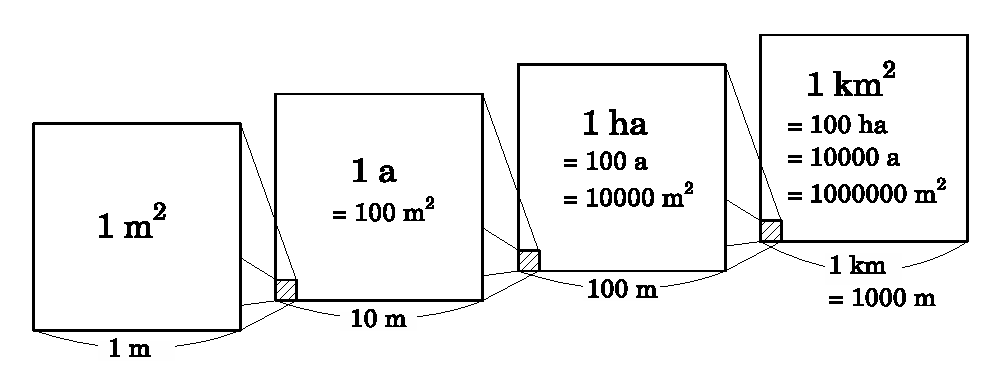
\includegraphics[width=8.2cm]{area_km2_ha.eps}
    \caption{いろいろな大きさの正方形の面積}\label{fig:area_km2_ha}
\end{figure}

\begin{q}\label{q:alg_unit1} 以下の量を書き換えよ:
\begin{edaenumerate}<2>
\item 1~mをkmで。
\item 1~kmをmで。
\item 1~cmをmで。

\item 1~m$^2$をkm$^2$で。
\item 1~km$^2$をm$^2$で。
\item 1~cm$^2$をm$^2$で。

\item 1~m$^3$をkm$^3$で。
\item 1~km$^3$をm$^3$で。
\item 1~cm$^3$をm$^3$で。

\item 1~dm$^3$をm$^3$で。
\item 1~dLをm$^3$で。
\item 1~$\mu$mをmで。

\item 1~$\mu$mをnmで。
\item 1~mgをkgで。
\item 1~km$^2$をhaで。
\end{edaenumerate}
\end{q}

{\small 注: dLは, 小学校以外ではほとんど使われない。これは, 1 dLの
立方体の1辺が, $(0.0001\,\text{m}^3)^{1/3}=0.0464\cdots$~mという
中途半端な数値になるからだろう。}

\begin{q}\label{q:alg_unit2} 以下の量を書き換えよ(導出過程も書け):
\begin{edaenumerate}
\item 0.009 km$^2$をm$^2$で。
\item 0.00003 km$^3$をm$^3$で。
\end{edaenumerate}
\end{q}

\begin{q}\label{q:alg_unit3} 以下の各小問内で, 挙げられた2つの単位が
互いに等しいことを示せ:
\begin{edaenumerate}
\item mLとcm$^3$。
\item Lとdm$^3$。
\item kLとm$^3$。
\item GtとPg。
\end{edaenumerate}
\end{q}

{\small 注: もともとLは「質量1~kgの水の体積」と定義されていたが, 
水は温度や圧力によって体積を微妙に変えるので, 体積の単位として
ふさわしくない。現在は, Lは10$^{-3}$~m$^3$のことであると
再定義され, なおかつ, 古い定義(水1~kgの体積)と紛らわしい
ので, Lはなるべく使わず, かわりにdm$^3$ (立方デシメートル)
と言おう, というのがSI単位系の立場である。\\}

SI単位系では他にもいろいろな約束が決まっている。特に, 
以下を覚えておこう:
\begin{itemize}
\item 変数や定数を表すアルファベットは斜体表記せよ。\\
例: $x=5$はOK, x$=5$はダメ。
\item 特定の関数を表すアルファベットは立体表記せよ。\\
例: $\sin x$はOK, $sin\,x$はダメ。
\item 単位を表すアルファベットは立体表記せよ。\\
例: 面積を表す$5\,\,\text{m}^2$はOK, $5\,\,m^2$はダメ。
\item 数値と単位の間には半角スペースをあけよ。\\
例: $5\,\,\text{m}^2$はOK, $5\text{m}^2$はダメ。
\item 組み立て単位は, 単位どうしの間に半角スペースをあけよ。\\
例: 速度を表す2 m~s$^{-1}$はOK, 2 ms$^{-1}$はダメ。
\item 接頭辞と単位の間にはスペースをあけるな。\\
例: 3~kgはOK, 3 k gはダメ。
\end{itemize}
最後の2つは特に大切。そのおかげで, 1~ms (1ミリ秒)
と1~m~s (1メートル秒)が区別できる。

科学技術文書のほとんどはこういう表記を使っている。
日本ではJIS規格になっている\footnote{しかし, なぜか日本の小中学校の検定教科書では, 
単位が斜体で書かれている。高校の教科書では立体になっているのだが...}。
本書も極力, この表記法に従う(一部, コンピュータソフトの仕様上の制限の為にうまく
できなかったところもあるが)。

レポートや卒業論文ではこれらに注意しよう。
ただし, 手書きでは無理に守らなくてもよい。
立体と斜字体の書き分けや, 「半角スペース」
は手書きでは無理だし。そこで, 手書きの時は, 
単位を括弧[ ]の中に入れて書いたりする。
例えば, 5.3~m/sを, 5.3~[m/s]と書くのだ。\\



\section{単位の換算}
\begin{exmpl}\label{exmpl:7.5km/h} 7.5 km~h$^{-1}$という量を, m~s$^{-1}$という単位に換算してみよう。
\begin{eqnarray}
7.5\,\,\text{km h}^{-1}&=&7.5\,\,\frac{\text{km}}{\text{h}}=7.5\,\,\frac{1000\text{ m}}{3600\text{ s}}\nonumber\\
&=&7.5\times\frac{1000}{3600}\text{ m s}^{-1}=2.08\cdots\text{ m s}^{-1}\nonumber\\
&\fallingdotseq&2.1\text{ m s}^{-1}
\end{eqnarray}
最後に2.08の8を四捨五入した。有効数字を考えたからである。7.5の有効数字が2桁であると判断されたので, 結果も有効数字2桁にした。\end{exmpl}

\begin{exmpl}\label{exmpl:2.0g/s} 2.0 g/sという量を, kg/hという単位で換算してみよう。
\begin{eqnarray}
&&2.0\,\,\text{g/s}=2.0\,\,\frac{\text{g}}{\text{s}}=2.0\,\,\frac{10^{-3}\text{ kg}}{(1/3600)\text{ h}}
=2.0\times\frac{3600}{1000}\text{ kg/h}\nonumber\\
&&=2.0\times3.6\text{ kg/h}=7.2\text{ kg/h}
\end{eqnarray}
(例おわり)\end{exmpl}\mv

これらの例でわかるように, 単位の換算は機械的にできる。
組み立て単位を構成する各単位(h, s, km, m, kg, gなど)を, 
それぞれ別の単位に換算し, そこで出てきた係数を計算すればよいのだ。\mv

上の例のやり方がよくわからない人には, かわりに, 
次の方法を勧める。例\ref{exmpl:7.5km/h}は,
\begin{eqnarray}
7.5\,\,\text{km h}^{-1}&=&7.5\,\,\frac{\text{km}}{\text{h}}\label{eq:unit_conv_mult1_02}\\
&=&7.5\,\,\frac{\text{km}}{\text{h}}\,\,\frac{1000\text{ m}}{\text{km}}\,\,\frac{\text{h}}{3600\text{ s}}\label{eq:unit_conv_mult1_04}\\
&=&7.5\,\,\frac{10\teisei{00}}{36\teisei{00}}\,\,\frac{\teisei{\text{km}}}{\teisei{\text{h}}}\,\,\frac{\text{ m}}{\teisei{\text{km}}}\,\,\frac{\teisei{\text{h}}}{\text{ s}}\label{eq:unit_conv_mult1_06}\\
&=&\frac{75}{36}\,\frac{\text{ m}}{\text{ s}}=2.08\cdots\text{ m s}^{-1}\\
&\fallingdotseq&2.1\text{ m s}^{-1}\label{eq:unit_conv_mult1_08}
\end{eqnarray}
ここで, \eref{eq:unit_conv_mult1_02}から\eref{eq:unit_conv_mult1_04}に行く時に, 
\begin{eqnarray}
\frac{1000\text{ m}}{\text{km}}\quad\text{と}\quad\quad\frac{\text{h}}{3600\text{ s}}\label{eq:unit_conv_times1}
\end{eqnarray}
をかけているが, これらは両方とも1だ。なぜなら, 1000~m=1~kmであり, 
両辺をkmで割ると, (1000~m)/km=1となる。同様にしてh/(3600~s)=1も言える。
これらの1は単位を持たぬ量(無次元量)だ。1を掛けても, 掛けられた量は何も
変化しない。そこで, \eref{eq:unit_conv_times1}のような, 「1と等しい量」
を自由にどんどん掛けて, 消し去りたい単位を約分していくのだ。

\begin{freqmiss}{\small\textgt{7.5~km/h = 27000000~m/sという, 
とんでもない間違いをする}... これは, 3600で割らねばならぬところを, 
3600を掛けてしまったミスです。この手のミスは, 計算過程で単位を埋め込まずに, 
数値だけで処理すると発生しがちです。でも, そもそも, 7.5~km/hは
徒歩(小走り)や自転車くらいの速さなので, 秒速2700万メートル
なんかになるわけがありません。\textgt{物理量を実際の現象と結びつけて
感覚的に把握する}習慣をつけましょう。}\end{freqmiss}

\begin{q}\label{q:unit_conv_mult1} 上で述べた, 1を掛けていく方法
で, 例\ref{exmpl:2.0g/s}の単位換算をやり直せ。\end{q}

\begin{q}\label{q:alg_unit4} 以下の量を書き換えよ。上で示した2つの方法の
どちらを使っても構わない。ただし, 導出過程も書くこと。電卓を使ってもOK。
\begin{enumerate}
\item 340~m/sをkm/hで。(音速)
\item $3.00\times10^8$~m/sをkm/hで。(光速)
\item 1.0~g/cm$^3$をkg/Lで。(水の密度)
\item 1.0~g/cm$^3$をt/m$^3$で。(水の密度)
\item 1.3~g/Lをkg/m$^3$で。(空気の密度)
\item 0.05~kg/hをg/sで。
\end{enumerate}
\end{q}
\mv

上のような問題では, 結果を科学の法則や現象に整合しているか
チェックしよう。例えば(1)は音速だが, 音速といえば飛行機だ。
音速を超えると急に抵抗が大きくなって燃料をたくさん喰う
ので, 多くの旅客機は音速より少し遅く飛ぶ。従って, 
(1)は, 旅客機が1時間で飛べる距離とだいたい同じはず。
飛行機に乗ったことのある人は, 旅客機は1時間で東京から九州とか
北海道の手前くらいまで飛ぶと知っているだろう。

\begin{q}\label{q:scale} 以下の量とおおよそ桁が合うような, 
具体的な現象や事物(数値を使わずに表現できるもの)
を述べよ。例: 1~ha ... 日本の平均的な農家1戸の耕作面積, 
1~L ... コンビニで売ってる中くらいの大きさのお茶のPETボトル。
\begin{edaenumerate}<3>
\item 1~mL
\item 1~m$^3$
\item 1~mg
\item 1~g
\item 1~kg
\item 1~t
\item 1~$\mu$m
\item 10000~km
\item 100000~km$^2$
\end{edaenumerate}
\end{q}
\mv

ところで, 物質の量は, 多くの場合は質量で表すが(「質量保存の法則」
があるから!), 体積で表すこともある。例えば3~tの水を
「3~m$^3$の水」と言ったりもする。すなわち, 
\begin{eqnarray}
3 \text{ t}\text{の水}=3 \text{ m}^3\text{の水}\label{eq:water_m3eq_t}
\end{eqnarray}
と言ってよい。だからといって, 
\begin{eqnarray}
\text{t}=\text{m}^3\quad\quad\text{(これは間違い!)}\label{eq:m3eq_t}
\end{eqnarray}
と言ってはダメ。そもそもtは質量, m$^3$は体積なのだから, これら
が同じなわけがない。もし\eref{eq:m3eq_t}が正しければ, 1~tの空気の体積も
1~m$^3$になってしまう(本当は約770~m$^3$)。\eref{eq:water_m3eq_t}が成り立つのは, 
水の密度がほぼ一定だからだ。密度が一定であれば, 質量と体積は
比例するから, どちらを使っても実用上は構わない。しかし, そこには
「密度」という重要な量が背後にあることを忘れてはダメ。


\begin{q}\label{q:rice_weight_vol} コメの量も, 重さ(質量)で
表したり, 体積で表したりする。コメのバルク密度を調べよ。(バルク
密度とは, たくさんの米粒を容器に入れた時のように隙間も含んだ
状態での密度)。それを元に, 10 kgのコメの体積を求めよ。\end{q}
%まだ答を作ってない!
\mv

\begin{faq}{\small\textgt{\eref{eq:water_m3eq_t}で両辺の「の水」を
約分すれば3~m$^3$=3~tになるから, \eref{eq:m3eq_t}も正しいのでは?}
 ... ダメ。約分は「何か×何か」の形の量について片方の「何か」
を割って消すこと。「3~m$^3$の水」は, 「3× 1~m$^3$の水」です。
1~m$^3$の水が3個分, という意味。でも君の考えでは, 
「3~m$^3$×水」と解釈して「水」だけを約分しています。これは無茶です。}
\end{faq}
\mv


\section{力の単位}

理系はどんな分野でも, 力やエネルギーの概念(中学理科の1分野)が
基礎だ。さらにその基礎は, 
\begin{itembox}{運動の法則(ニュートンの運動方程式)}
質量$m$の物体が力${\bf F}$を受けたとき, 物体の速度は変化する。
その変化率, つまり加速度(速度の変化を時間で割ったもの)を${\bf a}$とすると,
\begin{eqnarray}{\bf F}=m{\bf a}\label{eq:Newton_eqmotion}\end{eqnarray}
\end{itembox}
である。これは中学理科や高校の物理基礎で学んだ! これは全ての科学における
最も大切な常識のひとつである。この式を「知らない」という人がいるが, 
それは「細胞」とか「イオン」を知らないというくらいヤバい。

この式は, 本書の他の多くの数式とは根本的に性格が異なる。本書の多くの
数式は「定義」や「公理」か, それらをもとに導出される「定理」か, それらを
用いた計算式だ。ところが, この式はそのいずれでもない。
数式の格好をしているが, 自然の摂理を表す\underline{「基本原理」}
(基本法則ともいう)である。
そしてこの式の根拠は, 公理でも論理でもなく, 実験事実である。

ちなみに\eref{eq:Newton_eqmotion}で, ${\bf F}$はforce (力), 
$m$はmass (質量), ${\bf a}$はacceleration (加速度)
のそれぞれ頭文字から取られている。このように, 科学の
数式で出てくる記号は, その量の頭文字から取られることが多い。

\begin{freqmiss}{\small\textgt{「運動方程式を書け」という問に対して「${\bf F}=m{\bf a}$」とだけ答える}
 ... ${\bf F}, m, {\bf a}$のそれぞれが何を意味するかも, 書き添えなければなりません。}
\end{freqmiss}

\begin{faq}{\small\textgt{${\bf F}$と${\bf a}$の活字の形がなんか他と違うっぽいんですが...}
 ... よく気づきましたね。これは\pref{sect:vector_digest}あたりで学んだ「ベクトル」です。
力には大きさだけでなく向きもあるから, ベクトルです。加速度もそうです。だから, ベクトルの
書き方(太字)で書いているのです。}\end{faq}
\mv

さて, SI単位系では力の単位はN (ニュートン\footnote{いわずと知れた
イギリスの物理学者の名前。運動の法則と万有引力の法則
を発見した, 科学界のスーパースター。})である。\eref{eq:Newton_eqmotion}
において, ${\bf F}$をその単位であるNに置き換え, $m$をその単位であるkgで
置き換え, ${\bf a}$をその単位であるm s$^{-2}$で置き換えると, 
\begin{eqnarray}
\text{N}=\text{kg m~s}^{-2}\label{ed:def_N}
\end{eqnarray}
となる。これがNという単位の定義である。この式を忘れても, ${\bf F}=m{\bf a}$を覚えて
いれば, 上記のように考えればすぐに思い出せるだろう。

\begin{faq}{\small\textgt{加速度の単位がm s$^{-2}$, というのがわかりません。}
 ... 加速度は, ざっくりいうと, 速度の変化を時間で割ったものです(正確な定義は
後の章で説明します)。速度の単位はm s$^{-1}$ですから, 速度の変化(つまり, ある時刻の
速度ひく別の時刻の速度)の単位もm s$^{-1}$です。それを時間(単位はs)で割るのだから, 
最終的に単位はm s$^{-2}$になります。}\end{faq}

ところで, 「重さ」と「質量」を混同している人がいる。これはヤバイ。 重さは
その物体に働く重力のこと。重力は力の一種だ。だから重さは力の単位(SI単位系ではN)で表すのが, 科学的には正しい。
重さは場所によって変わる。同じ物体でも, 月面上での重さは地上での重さの
約1/6になるし, 国際宇宙ステーションの中(いわゆる無重力空間)
では重さは0~Nだ。

一方, 質量は, 力とは別の量だ。地球上だろうが月面上だろうが
無重力空間中だろうが, 同じ物体の質量は不変である。地球上で
1~kgの物体は, 月や国際宇宙ステーションに持って行っても1~kgなのだ。

えっ!? どういうこと!? と思う人は, ここから先を
慎重に読んでしっかり考え, 必ず理解しよう。まず質量
とは何だろう? それは\eref{eq:Newton_eqmotion}が教えてくれる。
\eref{eq:Newton_eqmotion}によると, 一定の力${\bf F}$を物体に
かけたとき, 質量$m$が大きい物ほど加速度${\bf a}$は小さいし, 
$m$が小さいほど${\bf a}$は大きいことがわかる。つまり質量$m$は
物体の「速度の変えにくさ」(加速度は速度が単位時間あたりに
どれだけ変化するか, という量であることに注意!), 
つまり「動かしにくさ」を表す。それは無重力空間でも変わらない。
国際宇宙ステーションの中に1~kgの物体と10~kgの物体の2つを
ぷかぷかと浮かせて, それらを同じ力で同じ時間だけ押すと, 
1~kgの物体の方がずっと速く飛んでいくだろう。

「重さ」の本質は, \eref{eq:Newton_eqmotion}とは別の
重要な物理法則が教えてくれる。それは, 「どんな物体どうしにも, 
互いに引き合う力が生じ, その大きさは, 2つの物体の質量の積に比例し, 
距離の2乗に反比例する」という法則だ。そのような力のことを重力と言うのだ。
地表で物体が地球から受ける重力は, その物体の質量と地球の質量の積に
比例し, 地球半径の2乗に反比例する。地球質量と地球半径はほぼ一定
なので, 「地表限定」の条件下では, 重力(つまり重さ)は, 物体の
質量だけで決まる。1~kgの物体の重さ(重力)は地表上のどこでも
約9.8~Nでほとんど変わらないので, 「1~kgの物体の地上での重さ」
を力の単位としてもよいだろう。そう定義された力の単位のことを, 
kgfという(kg重ともいう)。正確な定義では, 
\begin{eqnarray}
1 \text{ kgf}:=9.80665\text{ N}
\end{eqnarray}
である。実際, 土木や建築等の工学では力をkgfで表すことが多い。
しかし, kgfはSI単位系の単位ではないので, 科学ではkgfを使うことは
避ける方がよい。

ところで, 世の中では往々にしてkgfのfが略されて「kg」と言われて
しまう。一方, 日常生活では, 質量と重さは頻繁に混同され, 「A君の
体重は60~kg」というような表現が多い。でも体重とは「体の重さ」
なので, 正しくは「A君の体重は60~kgf」もしくは「A君の質量は60~kg」
とすべきである。

日常生活では体重と質量を混同したり, kgfをkgと誤記しても困らないので, 
そんなにこだわる必要は無い。しかし科学の世界では, 明確に区別
せねばならない。\mv

\begin{faq}{\small\textgt{中学校で, 「100 g = 1 N 」と
習ったのですが...} ... それは間違い。100~gは質量, 1~Nは
力なので, 両者は互いに次元が異なるから, 等号で結ぶことは
できません。ただ, 「質量100~gの物体\textgt{にかかる重力の大きさ}
は約1~Nである(正確には0.98~N)」というのは正しいし, 私が
チェックした中学校の教科書にはそのように載っていました。
「100 g = 1 N 」のような乱暴な間違いが載っているのは, 
塾のプリントや参考書のようです。\\
\textgt{それのどこがダメなのか, いまいちわかりません...} ... 
例えで説明しましょう。1~Lの水の質量は(ほぼ)1~kgです。
だからといって、 1~L=1~kgと言ってはダメでしょう。
左辺は体積, 右辺は質量なのだから。それと同じこと。}\end{faq}

\begin{q}\label{q:kgf} 60~kgfは何Nか? 有効数字2桁で。\end{q}
\hv


\section{エネルギーと圧力の単位}\label{sect:energy_pressure}

次に, 仕事とエネルギーの定義を確認しよう。これらも中学校理科であり, 
知らなきゃヤバイことである:
\begin{itembox}{仕事とエネルギーの定義} 
物体に力をかけて移動させるとき, 力と, その力の方向に動いた
距離との積を, 「仕事」\index{しごと@仕事}という。仕事と等価な量(仕事に形を
変えることができる量)のことを「エネルギー」\index{えねるぎー@エネルギー}という。
\end{itembox}

ざっくり言えば, 「仕事=力×距離」である。SI単位系では, 仕事の単位は
J (ジュール\footnote{イギリスの物理学者の名前。電気回路で
出る熱に関する「ジュールの法則」を発見した人。})だ。
「仕事=力×距離」で, 「仕事」をその単位であるJで置き換え, 「力」を
その単位であるNで置き換え, 「距離」をその単位であるmで置き換えれば, 
\begin{eqnarray}
\text{J}=\text{N m}\label{ed:def_J}
\end{eqnarray}
となる(定義)。\eref{ed:def_J}を忘れても, 「仕事=力×距離」
を覚えていれば, 思い出せるだろう。\\

エネルギーは仕事と等価な量なので, エネルギーのSI単位は仕事と同じJである。\\

また, 中学校理科で学んだように, 面に一様に力がかかるとき, 
その力を面積で割ったものを圧力という。ざっくり言えば, 
「圧力=力/面積」だ。SI単位系では, 圧力の単位はPa (パスカル
\footnote{フランスの哲学者かつ物理学者の名前。「人間は考える葦である」
との言葉を残した人。})である。
「圧力=力/面積」で, 「圧力」をその単位であるPaで置き換え, 「力」を
その単位であるNで置き換え, 「面積」をその単位であるm$^2$で置き換えれば, 
次式になる:
\begin{eqnarray}
\text{Pa}=\text{N/m}^2=\text{N m}^{-2}\label{ed:def_Pa}
\end{eqnarray}
これがPaの定義である。\eref{ed:def_Pa}を忘れても, 「圧力=力/面積」
を覚えていれば, 思い出せるだろう。\\

また, 中学校理科で学んだように, ある時間内になされた仕事や, 出入りした熱や, 
エネルギーの増減量を, その時間で割ったものを, 仕事率又は熱効率という。
ざっくり言えば, 「仕事率=仕事/時間」である。SI単位系では, 
仕事率の単位はW (ワット\footnote{イギリスの発明家の名前。
蒸気機関を開発して, 産業革命に貢献した人。})である。
「仕事率=仕事/時間」において, 「仕事率」をその単位であるWで置き換え, 
「仕事」をその単位であるJで置き換え, 「時間」をその単位であるsで置き換えれば, 
\begin{eqnarray}
\text{W}=\text{J/s}=\text{J s}^{-1}\label{ed:def_W}
\end{eqnarray}
となる。これがWの定義である。\eref{ed:def_W}を忘れても, 「仕事率=仕事/時間」
を覚えていれば, 思い出せるだろう。

\begin{freqmiss}{\small\textgt{WとJを混同する} ... 
JとWは明確に異なる単位です。W=J/s, J=W sです。}\end{freqmiss}

ところで, 電気的なエネルギーや電気がする仕事を「電力量」\index{でんりょくりょう@電力量}という。また, 
電気がする仕事の仕事率を「電力」\index{でんりょく@電力}という。

\begin{freqmiss}{\small\textgt{Wは電気専用の単位だ
と思っている} ... 
Wは仕事率の単位なので, 電力以外の仕事率にも使われます。
おそらくこういう誤解をする人は, 中学校で習った
W=A$\times$V (Aはアンペア, Vはボルト)に引きずられて
いるのでしょう。それは間違いではないけど, Wの定義では
ありません。}\end{freqmiss}

\begin{q}\label{q:state_F=ma_etc} 
\begin{enumerate}
\item ニュートンの運動方程式を書け。
\item 仕事の定義を書け。
\item エネルギーの定義を書け。
\item 圧力の定義を書け。
\item 仕事率の定義を書け。
\end{enumerate}\end{q}

\begin{q}\label{q:unit_NJPaW_matome7} 以下の問に答えよ。
導出過程も書くこと。
\begin{enumerate}
\item 質量2$\,\,$kgの物体を加速度3 m~s$^{-2}$で加速するのに必要な力は?
\item ある物体を2 Nの力で4 mだけ移動させるのに必要なエネルギーは?
\item 2$\,$m$^2$の平面に10$\,$Nの力がかかっている状態の圧力は?
\item 100$\,\,$Wの電球が, 2秒間に消費する電力量は?
\end{enumerate}
\end{q}

\begin{q}\label{q:unit_NJPaW_relation} 以下を示せ:
\begin{edaenumerate}
\item N = J / m
\item Pa = J~m$^{-3}$
\item J = Pa~m$^3$
\item J/Pa = m$^3$
\item W = N~m~s$^{-1}$
\item J = W~s
\end{edaenumerate}
\end{q}
\mv

\begin{q}\label{q:unit_NJPaW_matome1} J, Pa, Wを, 
それぞれSI基本単位(kg, m, s)の組み合わせで表わせ。\end{q}

\begin{q}\label{q:kWh2J_hPa2Pa} 以下の量を書き換えよ:
\begin{edaenumerate}
\item 1~kW hをJで。
\item 1~hPaをPaで。
\end{edaenumerate}
\end{q}
\mv

ところで, 圧力の単位にatm (気圧)というのがある。定義は
$1\text{ atm} :=1013.25\text{ hPa}$である
(hPaのhを忘れる人が多い)。atmはatmosphereの略である。
1~atmのことを1~気圧ともいう。

\begin{q}\label{q:unit_atm_Pa_conversion} 以下の問に答えよ。電卓を使ってもよい。
\begin{enumerate}
\item 1~atmをPaで表わせ。
\item 1~atmをkPaで表わせ。
\item 1~Paをatmで表わせ。
\item ある巨大な台風(実際にあった!)の中心付近での地表での気圧は895~hPaだった。
この圧力をatmで表わせ。
\end{enumerate}
\end{q}

高校の化学や物理で学んだように, 理想気体の圧力$P$, 体積$V$, 
モル数$n$, 絶対温度$T$, 気体定数\index{きたいていすう@気体定数}$R$の間には, 
$PV=nRT$という関係が成り立つ(理想気体の状態方程式)。また, $R=8.3145~\text{J~mol}^{-1}\text{K}^{-1}$
である。

\begin{q}\label{q:PVnRT} 1.0000~molの理想気体が, 温度273.15 K, 
1013.25 hPaにあるときの体積を計算し, Lで表せ。電卓使用可。\end{q}

\begin{q}\label{q:gas_const_conversion} 気体定数$R=8.3145$~J~mol$^{-1}$~K$^{-1}$
の値を, atm~L~mol$^{-1}$~K$^{-1}$という単位で書き換えよ。
電卓使用可。途中経過も書け。ヒント: J=Pa~m$^3$。\end{q}

ところでエネルギーの単位にカロリー(cal)というのもある。
定義は, $1\text{~cal}:=4.184\text{~J}$である(記憶せよ)。もともと, 
1~calは「質量1~gの水の温度を1$^\circ$C上げるのに必要
な熱量」と定義されていたのだが, それは条件次第で
微妙に異なるので, 今は上のようにJとの関係で定義されている。

\begin{q}\label{q:water_specific_heat} 常温・液体の
水の比熱を, J kg$^{-1}$ K$^{-1}$という単位で表わせ。
\end{q}

\begin{q}\label{q:cal_J} 以下の問に答えよ:
\begin{enumerate}
\item 成人ひとりが1日に食物から摂取するエネルギーは約2500~kcal
である。この量をJで書き換えよ。
\item 上記のエネルギーを全部熱にすると, 体積0.5~m$^3$の水
(風呂桶1杯くらい!)の温度を何Kだけ上げることができるか?
\item 上記のエネルギーを全部仕事にすると, 質量10~kgの
物体を地上からどのくらいの高さまで持ち上げることができるか?
\end{enumerate}
\end{q}
\mv

\begin{comment}
\section{物理量を表す記号}

\eref{eq:Newton_eqmotion}で$F=ma$が出てきたとき, 
$F$は力, $m$は質量, $a$は加速度だった。でも, 例えば
力を$A$, 質量を$B$, 加速度を$C$とすれば, 
\eref{eq:Newton_eqmotion}は$A=BC$と書いても構わない。
このように, 原則的には, 物理量は, 各自が記号を自由に定義して使ってよいのだ。

でも, 規則ではないが「この物理量はこの記号を使うのが普通だよね」
という慣習というか常識というか空気がある。いわば, 犬の名前はポチ, 
猫の名前はタマ, みたいなものだ。その代表的なものを以下に示す:

\begin{table}[!htb]\caption{物理量の慣習的な記号と単位}
\begin{center}
\begin{tabular}{ccc}\hline
物理量 & 記号 (由来) & 単位 \\\hline
質量 & $m$ (mass) & kg \\
時刻 & $t$ (time) & s \\
長さ, 位置 & $l$ (length), $x$等 & m \\
面積 & $a$, $A$ (area), $S$ (surface) & m$^2$ \\
体積 & $V$ (volume) & m$^3$ \\
速度 & $v$ (velocity) & m s$^{-1}$ \\
加速度 & $a$ (acceleration) & m s$^{-2}$ \\
力 & $F$ (force) & N \\
仕事 & $w$, $W$ (work) & J \\
仕事率 & $P$ (power) & W \\
圧力 & $p$, $P$ (pressure) & Pa \\
分子数 & $n$, $N$ (number) & 個, 又はmol \\
熱量 & $q$, $Q$ & J \\
エネルギー & $E$ (energy), $U$, $K$, $T$& J \\
温度 & $T$ (temperature) & K \\\hline
\end{tabular}
\end{center}
\end{table}
これらは覚えなくてもよいが, 慣れるのが望ましい。
紛らわしいのが, 別々の物理量の記号と単位に同じようなアルファベット
が現れる場合。例えば$m$は質量を表す一方, mは長さの単位である。
$W$は仕事を表す一方, Wは仕事率の単位である。しかし
こういうのは, 物理量は斜字体, 単位は立体, という, 
字体の用法で区別できる。だから字体は大事なのだ。

また, 同じ記号が, 違う物理量に出てくる(かぶる)ことも
ある。例えば$P$は, ときに仕事率, ときに圧力を表す。だから, 
物理量の記号は, たとえ「それが常識」でも, 毎回その場その場で
定義し直さねばならない。\\
\end{comment}

\section{dimension check}
ここで, ひとつ, 便利な道具を紹介しよう。

\begin{exmpl}
高校の物理基礎で学んだように, 質量$m$の物体が速さ$v$で移動しているとき, 
その物体の持つ運動エネルギー$K$を次式で定義する:
\begin{eqnarray}
K:=\frac{1}{2}m\,v^2\label{eq:def_kinenergy}
\end{eqnarray}
この両辺の単位をSI単位で考えよう。まず1/2は無次元量なので
単位なし。$m$の単位はkg, $v^2$の単位は(m s$^{-1}$)$^2$=m$^2$~s$^{-2}$。
従って, 右辺の単位はkg m$^2$~s$^{-2}$。これはJである
(問\ref{q:unit_NJPaW_matome1}参照)。一方, 左辺の$K$は
「エネルギー」と呼ばれる以上, SI単位ではJで表現できる
はずである。従って, この両辺は, 同じ単位で揃えることが
できる(次元が同じ!)。(例おわり)\end{exmpl}

このように, ある式について, 両辺が同じ単位を持てるかを調べること
(すなわち両辺で次元が一致しているか調べること)を, 
dimension check\index{dimension check}という。
等式の両辺は, 互いに同じ物理量を表すのだから, 
同じ単位で表すことができる(次元が一致している)はず。
ところが, 何かミスをすると(例えば\eref{eq:def_kinenergy}
の$v^2$の2乗を忘れたり), 左辺と右辺で単位は一致
しなくなることが多いので, これは, その式が正しく
できているかどうかの検算に使える。

実は, これに似た考え方を, 既に例\ref{exmpl:niku600yen}や
例\ref{exmpl:mihaji}で紹介した。つまり, 単位を式に埋め込んで
計算すれば, 結果的にdimension checkにもなるのだ。\mv

\begin{q}\label{q:unit_dimcheck} \eref{eq:rect_area00_NG}
のような書き方が不合理であることを, dimension checkの観点で
説明せよ。\end{q}

\begin{q}\label{q:potentialE_dim} 高校の物理基礎で学んだように, 
地表付近で, 質量$m$の物体が高さ$h$にあるとき, その物体の持つ
位置エネルギー$U$は次式で表される\footnote{これは位置エネルギー
の定義ではない。位置エネルギーは, これとは別の式で定義され, そこから
この式が演繹される。また, 大学では位置エネルギーを
「ポテンシャルエネルギー」と呼ぶ。}。
\begin{eqnarray}
U=mgh
\end{eqnarray}
$g$は重力加速度と呼ばれる定数で, $g\fallingdotseq9.8$~m~s$^{-2}$である。
この式をdimension checkせよ。
\end{q}

\begin{q}\label{q:sphere_SV_dimcheck} 半径$r$の球の
表面積$S$と体積$V$はそれぞれ
\begin{eqnarray}
&&S=4\pi r^2\label{eq:ball_surface}\\
&&V=\frac{4}{3}\pi r^3\label{eq:ball_volume}
\end{eqnarray}
である。ところが, 君の友人A君は, この公式を逆に
覚えている($V=4\pi r^2$, $S=4\pi r^3/3$と覚えている)。
dimension checkを使って, A君に間違いを
教えてあげるには, どう言えばよいか?
\footnote{$S$はsurfaceの頭文字, $V$はvolumeの頭文字, 
そして$r$はradiusの頭文字に由来する。このように, 
量を表す記号(アルファベット)は, その英単語に
由来することが多い。それも公式を覚えたり思い出したり
するときの手がかりになる。}\end{q}

%\begin{q}\label{q:dim_fric_coeff} ある物体が別の物体と接触して, 互いに摩擦を及ぼしながら
%動いているとき, 両者にかかる摩擦力を$F_{\text{m}}$とすると, それは
%接触面を介して両者が互いに垂直に押し合う力$N$に比例する, ということが
%わかっている(クーロンの摩擦法則の一部)。すなわち, 
%\begin{eqnarray}F_{\text{m}}=\mu'N\label{eq:law_friction_m}\end{eqnarray}
%と書ける。このときの比例係数$\mu'$のことを「動摩擦係数」と呼ぶ。
%動摩擦係数の次元は無次元であることを示せ。\end{q}
\hv


\section{例外!}
ここで, 少しやっかいな話。「物理量は数値と単位の積」
と述べたが, そうではない場合が存在するのだ。

もし物理量が「数値と単位の積」なら, その「数値」が0の
ときにはその物理量は0である。例えば, 0 mは長さが0 (無い)
ということである。

すると, 「数値が0でも物理量が0にならない場合」は, 
「数値と単位の積」ではない, ということになる(これは上
で述べたことの対偶である。対偶がわからない人は, 
索引で調べよ)。そして, 実際にそのような場合があるのだ!

\begin{exmpl} 温度はそもそも, 分子の平均運動エネルギー
に比例するような物理量であり, その単位としてK (ケルビン)
が使われる。当然, 分子の平均運動エネルギーが0
のときの温度は0 Kである。ところが, 温度を摂氏で表すと, 
$0\ {}^\circ\mathrm{C}$のときは273~Kであり, 0~Kではない。
\end{exmpl}

\begin{exmpl} pHは, 水溶液の中の
水素イオンの濃度\index{すいそいおんのうど@水素イオン濃度}[H$^+$]
の指標であり, 次式で定義される:
\begin{eqnarray}
\text{pH}:=-\log_{10}\frac{\text{[H}^+\text{]}}{\text{mol~L}^{-1}}\label{eq:define_pH}
\end{eqnarray}
%[H$^+$]が$10^{-7}\,\,$mol L$^{-1}$である水溶液のpHは7であり, 
%[H$^+$]10倍になるたびにpHは1下がる, と約束する。例えば, 
%pHが5の水溶液は[H$^+$]=$10^{-5}\,\,$mol~L$^{-1}$である。
\end{exmpl}

\begin{q}\label{q:pH2density} 次式を示せ:
\begin{eqnarray}
\text{[H}^+\text{]}=10^{-\text{pH}}\text{ mol~L}^{-1}\label{eq:pH2density}
\end{eqnarray}
\end{q}

\begin{q}\label{q:pH0} pHが$-1$の水溶液の水素イオン濃度は?\end{q}

\begin{q}\label{q:exp_pH} 
\begin{enumerate}
\item 水素イオン濃度が0.005 mol~L$^{-1}$のときpHは?
\item pH=5.6のとき, 水素イオン濃度は中性(pH=7)のときの何倍か? 
\item pH=5.0の塩酸と, pH=3.0の塩酸を, 等量, 混ぜ合わせたら, 
pHはどのくらいになるか? ただし塩酸はすべて解離するものとする。
\end{enumerate}\end{q}

%\begin{exmpl} 君が受験でお世話になった「偏差値」は, 個々の学生
%の成績が, 受験生全体の中でどのくらいかを表す(その定義は本書の後半
%で学ぶ)。ところが, 得点が0点でも偏差値30とか40ということはよくある。
%(例おわり)\end{exmpl}

ここで示した2つの例は, 「数値と単位の積」ではない。つまり, 
$\ {}^\circ\mathrm{C}$やpHという単位は, 普通じゃない, 
変な単位である。こういう単位は, 単位同士の掛け算, 割り算, 約分
はできないし, それを利用した単位換算法も使えないし, 
\eref{eq:L/cm=15}のような表現もできないし, dimension checkも使えない。
なので, こういう単位のからむ計算や変換は, ケースバイケースで慎重に
対応しなければならない。

\begin{faq}{\small\textgt{「ケースバイケースで慎重に対応」って, 
具体的にはどういうことですか?}... いちばん簡単なのは, 単位換算や
他の量と一緒に計算する時にはそういう量を「数値と単位の積」
に書き換えてしまうことです。$\ {}^\circ\mathrm{C}$は
Kに, pHはmol L$^{-1}$に書き換えてしまうのです。}\end{faq}


%同様の事情は, 地震の規模を表すマグニチュード\index{まぐにちゅーど@マグニチュード}
%という指標や, 音の大きさを表すデシベル\index{でしべる@デシベル}という指標にもある。
%これらの特殊な単位には, 「対数」という考え方が背景にある(対数については第\ref{chapt_exp_log}章で学ぶ)。\\
%\hv

% 摂氏とK。
% 0度C=273Kの両辺を2倍したら, 0度C=546K。何がおかしい?
% 度CとKは比例しない。
% 同じことが摂氏と華氏でも起きる。
% 度Cは「単位」とは言えない。
% 例: 100点満点のテスト。40点=偏差値50。両辺を2倍したら, 80点=偏差値100? 何かおかしい。
% 得点と偏差値は比例しない。
% 同じ対象でも, 表現の仕方によって, 数学的な性質が大きく異なる。そういう場合はイコールで結んではいけない(おかしなことになる)。
\mv


\section*{演習問題}

\begin{exq}\label{q:degC_K} $0\ {}^\circ\mathrm{C}$は273 Kである。
つまり, 
\begin{eqnarray}
0\ {}^\circ\mathrm{C}=273\text{ K}
\end{eqnarray}
である。ところが, この両辺を2倍すると, 
\begin{eqnarray}
0\ {}^\circ\mathrm{C}=546\text{ K}
\end{eqnarray}
になってしまう。この2つの式に\eref{eq:equality03}を使うと, 
\begin{eqnarray}
273\text{ K}=546\text{ K}
\end{eqnarray}
となってしまう。どこでどのように間違ったのか?
\end{exq}

\begin{exq}\label{q:unit_old} 生物資源学類で農業を学ぶとき, 古い単位が
出てくることがよくある。以下のそれぞれの単位について, その由来と, 
相互の関係, そしてSI基本単位でどのくらいかを調べよ:\\
長さの単位: 寸, 尺, 丈, 間, 町, 里\\
面積の単位: 畳, 坪, 畝, 反, 町\\
体積の単位: 合, 升, 斗, 石\\
質量の単位: 貫
\end{exq}

\begin{exq}\label{q:unit_missing} 伝統的に, 生物資源学類生の
多くには, 教員がテキスト・プリント・口頭で繰り返し注意しても, 必要な単位
を付け忘れるという性質がある。「単位の付け忘れ」に関する君の体験を
述べ, このミスを解消できる, 人道的で手間と費用の少ない教育法を提案せよ。
ちなみに「テストで減点」とか「呼び出して説教」というのはあまり効果
が無いことがわかっている。また, 「テストの解答用紙に単位を書く欄
を設ける」とか, 「テストのたびに, 単位を忘れないように注意を与える」
などはむしろ, 自主的に単位をつけようとする態度や習慣の成長を阻害
する可能性がある。
\end{exq}

\begin{faq}{\small\textgt{教育とは手間のかかるものだと思います}
 ... それは一般論として正しいけど, 「単位の付け忘れ」は
小中学校で矯正されるべきですし, 自分でも「単位つけないのはまずくね?」
と気づくべきことです。大学がわざわざ「手間をかけて教育」するような
ことではありません。}\end{faq}

\begin{faq}\small{\textgt{テストとかで後から見ると信じられないようなミスをします。
ミスを減らす方法ってありますか?}
... 人間だからミスはなかなか無くせないですよね。むしろミスしてミスから
学ぶのです。ただし, ミスを指摘されているのに気付かずに同じミスを
繰り返したり, 最初からテキストで注意喚起されているところをミスするのはダメです。}\end{faq}
\mv


\section*{問の解答}

\noindent{\textbf{答}}\ref{q:alg_dim00} 「お互いに単位を
揃えることができるかどうか」という観点で共通する性質。\mv

\noindent{\textbf{答}}\ref{q:unit_mihaji} 
\begin{eqnarray*}
&&\text{(1)}\quad\frac{500\text{ リットル}}{5\teisei{\text{ 時間}}}\times 2\teisei{\text{時間}} = 200\text{ リットル}\\
&&\text{(2)}\quad\frac{5\text{ 時間}}{500\text{ リットル}}\times 4{\text{ m}^3}\\
&&\quad\quad=\frac{5\text{ 時間}}{500\teisei{\text{ リットル}}}\times 4\times 10^3\teisei{\text{ リットル}}=40\text{ 時間}\\
&&\text{(3)}\quad\frac{21000\text{ t}}{4900\text{ ha}}=\frac{21000\times10^3\text{ kg}}{4900\times10^4\text{ m}^2}
=\frac{2.1\times\teisei{10^7}\text{ kg}}{4.9\times\teisei{10^7}\text{ m}^2}\\
&&\quad\quad\fallingdotseq0.43\text{ kg/m}^2\\
&&\text{(4)}\quad\text{(3)の逆数。 }
\quad 1/(0.43\text{ kg/m}^2)\fallingdotseq 2.3\text{ m}^2\text{kg}^{-1}\\
&&\text{(5)}\quad0.43\,\frac{\text{kg}}{\teisei{\text{m}^2}}\times260\times10^4\,\teisei{\text{m}^2}\fallingdotseq110\times10^4\text{ kg}
=1100\text{ t}\\
&&\text{(6)}\quad 60\,\frac{\teisei{\text{kg}}}{\teisei{\text{人}}}\times130\,\teisei{\text{人}}\times2.3\frac{\text{ m}^2}{\teisei{\text{kg}}}
\fallingdotseq 18000\text{ m}^2 = 1.8\text{ ha}\\
&&\text{(7)}\quad 120\text{ ha}
\times\frac{2.5\text{ トン}}{1\text{ ライ}}
\times\frac{4.4\teisei{\text{ バーツ}}}{1\text{ kg}}
\times\frac{100\text{ 円}}{33\teisei{\text{ バーツ}}}\\
&&=
120\times 10^4\teisei{\text{ m}^2}
\times\frac{2.5\times10^3\teisei{\text{ kg}}}{1600\teisei{\text{ m}^2}}
\times\frac{4.4}{1\teisei{\text{ kg}}}
\times\frac{100\text{ 円}}{33}\\
&&=2.5\times 10^7\text{ 円}
(=2500\text{ 万円})
\end{eqnarray*}

%\noindent{\textbf{答}}\ref{q:SIunit} 略(本文に書いてある)。\mv

\noindent{\textbf{答}}\ref{q:nonSIunit} (略解) いずれも, kg, m, sの3つの単位のどれかで表すことができる。
(1) 60 s。(2) 3600 s。(3) 100~m$^{2}$。以下, 略。\mv

%\noindent{\textbf{答}}\ref{q:SIsettouji} 略(本文に書いてある)。\mv

\noindent{\textbf{答}}\ref{q:alg_unit1} (略解)\\
(1) 1~m=10$^{-3}$~km。1~m=0.001~kmと書いてもOK。\\
(4) 1~m$^2$=1 $\times$ (10$^{-3}$ km)$^2$=10$^{-6}$~km$^2$。\\
(8) 1~km$^3$=1$\times$(10$^3$~m)$^3$=10$^{9}$~m$^3$。\\
(11) 1 dL=10$^{-1}$~L=10$^{-1}\times10^{-3}$~m$^3$=$10^{-4}$~m$^3$。他略。

\noindent{\textbf{答}}\ref{q:alg_unit2} (略解) (1) $9\times 10^3$~m$^2$。(2) $3\times 10^4$~m$^3$。
\mv

\noindent{\textbf{答}}\ref{q:alg_unit3} (略解) \\
(1) mL=$10^{-3}$~L = $10^{-3}\times10^{-3}$~m$^3$=$10^{-6}$~m$^3$。cm$^3$=(10$^{-2}$~m)$^3$=$10^{-6}$~m$^3$。よって, mL = cm$^3$。\\
(2), (3)は略。
(4) Gt=$10^9\times10^3$~kg=$10^{12}$~kg。Pg=$10^{15}$~g=$10^{12}$~kg。よって, Gt=Pg。\mv

\noindent{\textbf{答}}\ref{q:unit_conv_mult1} 
\begin{eqnarray*}
&&2.0\,\,\text{g/s}=2.0\,\,\frac{\text{g}}{\text{s}}
=2.0\,\,\frac{\text{g}}{\text{s}}\frac{\text{kg}}{1000\text{ g}}\frac{3600\text{ s}}{\text{h}}\\
&&=2.0\,\,\frac{\teisei{\text{g}}}{\teisei{\text{s}}}\frac{\text{kg}}{1000 \teisei{\text{ g}}}\frac{3600\teisei{\text{ s}}}{\text{h}}
=\frac{2.0\times3600}{1000}\frac{\text{kg}}{\text{h}}
=7.2\text{ kg/h}
\end{eqnarray*}

\noindent{\textbf{答}}\ref{q:alg_unit4} (略解) \\
(1) 1220~km/h。(有効数字3桁とみなした。4桁で1224~km/hでもOK)。\\
(2) 1.08$\times 10^9$~km/h。
(3) 1.0~kg/L。
(4) 1.0 t/m$^3$。
(5) 1.3~kg/m$^3$。
(6) $1.4\times 10^{-2}$~g/s。\mv

\noindent{\textbf{答}}\ref{q:scale} 与えられた量に
対して0.5倍から数倍の違いがある事物でOK(ざっくり!)。
以下は例。レポートではここに挙げた例を答えてはならない。
\begin{enumerate}
\item 1 mL ... インフルエンザワクチンの容量(0.5~mL)。
\item 1 m$^3$ ... 銭湯の小さめの浴槽の容量。
\item 1 mg ... キイロショウジョウバエ1匹の質量。
\item 1 g ... 1円玉1個の質量。
\item 1 kg ... サッカーボールの質量(0.5~kg)。
\item 1 t ... 軽自動車1台の質量。
\item 1 $\mu$m ... 大腸菌1匹の大きさ。
\item 10000~km ... 地球の直径(13000~km)。
\item 100000~km$^2$ ... 北海道の面積(83500~km$^2$)。
\end{enumerate}

%\noindent{\textbf{答}}\ref{q:rice_weight_vol} 略。

\noindent{\textbf{答}}\ref{q:kgf} $60\times 9.8\text{ N}\fallingdotseq590\text{ N}$

%\noindent{\textbf{答}}\ref{q:state_F=ma_etc} 略(本文に書いてある)。


% section{力・エネルギー・圧力}

\noindent{\textbf{答}}\ref{q:unit_NJPaW_matome7}
\begin{enumerate}
\item 2~kg$\times$ 3~m~s$^{-2}$=6~kg~m~s$^{-2}$ = 6~N
\item 2~N$\times$4~m = 8~N~m = 8~J
\item (略解) 5~Pa
\item (略解) 200~J
\end{enumerate}


\noindent{\textbf{答}}\ref{q:unit_NJPaW_relation}(略解)\\
(1) J = N~mの両辺をmで割る。(2) Pa=N/m$^2$の右辺に, 前小問で示したN=J/mを代入。
(3)以下は略。\mv

\noindent{\textbf{答}}\ref{q:unit_NJPaW_matome1} \eref{ed:def_J}の右辺の
Nに\eref{ed:def_N}を代入すると, 
\begin{eqnarray}
\text{J=kg m s}^{-2}\text{ m=kg m}^2\text{ s}^{-2}\label{eq:J_kgms}
\end{eqnarray}
\eref{ed:def_Pa}の右辺のNに\eref{ed:def_N}を代入すると, 
\begin{eqnarray}
\text{Pa=kg m s}^{-2}\text{/m}^2\text{=kg m}^{-1}\text{ s}^{-2}\label{eq:Pa_kgms}
\end{eqnarray}
\eref{ed:def_W}の右辺のJに\eref{eq:J_kgms}を代入すると, 
\begin{eqnarray}
\text{W=kg m}^2\text{ s}^{-2}/\text{s}\text{=kg m}^2\text{ s}^{-3}\label{eq:W_kgms}
\end{eqnarray}

\noindent{\textbf{答}}\ref{q:kWh2J_hPa2Pa}
(1) 1~kW h = ($10^3$ W)$\times(3600$~s) = 3.6$\times 10^6$ W~s = 3.6$\times 10^6$ J。
(2) 1 hPa = 10$^2$ Pa = 100 Pa。\mv

%\noindent{\textbf{答}}\ref{q:dim_fric_coeff}
%\begin{eqnarray}
%[\mu']=\Bigl[\frac{F_{\text{m}}}{N}\Bigr]=\frac{[F_{\text{m}}]}{[N]}=\frac{[\text{力}]}{[\text{力}]}
%\end{eqnarray}
%となる。つまり, 同じ次元の量どうしの比であり, それらは互いに打ち消しあう。従って
%[動摩擦係数]は無次元。\mv

\noindent{\textbf{答}}\ref{q:unit_atm_Pa_conversion} \\
(1) $1\text{ atm} :=1013.25\text{ hPa}=1.01325\times10^3\times10^2\text{ Pa}$
$=1.01325\times10^5\text{ Pa}$。\\
(2) 1~atm=$101.325\times 10^3$~Pa=101.325~kPa\\ 
(3) (1)より, 1 Pa$=1/(1.01325\times10^5)$ atm
= 9.86923$\times10^{-6}$ atm。\\
(4) 895 hPa = 895$\times 10^2\times 9.86923\times10^{-6}$ atm\\
 = 0.883 atm。\mv

\noindent{\textbf{答}}\ref{q:PVnRT}
\begin{eqnarray*}
V&=&\frac{nRT}{P}\\
 &=&\frac{1.0000\text{ mol}\times 8.3145\text{ J mol}^{-1}\text{K}^{-1} \times 273.15\text{ K}}{1.01325\times10^5\text{ Pa}}\\
&=&\frac{8.3145\times 273.15\text{ J} }{1.01325\times10^5\text{ Pa}}=2.2414\times10^{-2}\text{ J/Pa}\\
&\fallingdotseq& 2.2414\times10^{-2} \text{ m}^3=2.2414\times10^{-2}\times10^{3}\text{ L}\\
&=&22.414\text{ L}
\end{eqnarray*}
なお, J/Paをm$^3$に置き換えたところがわからない人は, 問\ref{q:unit_NJPaW_relation}(4)を参照せよ。\\

\noindent{\textbf{答}}\ref{q:gas_const_conversion} 
問\ref{q:unit_NJPaW_relation}(3)より, J=Pa~m$^3$。また, m$^3$=10$^3$~L。\\
従って, J=10$^3$ Pa~L。また, 問\ref{q:unit_atm_Pa_conversion}より, \\
Pa = 9.86923$\times10^{-6}$ atm。従って, \\
J=$10^3\times 9.86923\times10^{-6}$ atm~L=$9.86923\times10^{-3}$ atm~L。
従って, $R=8.3145 \text{ J~mol}^{-1}\text{K}^{-1}$\\
$=8.3145\times 9.86923\times10^{-3} \text{ atm~L~mol}^{-1}\text{ K}^{-1}$\\
$=0.082058\text{ atm~L~mol}^{-1}\text{ K}^{-1}$。\\

\noindent{\textbf{答}}\ref{q:water_specific_heat} 物質を温める
ときに, 投入した熱量を$Q$, 温度変化を$\Delta T$, 質量を$m$とすると, 
比熱は$Q/(m\Delta T)$と定義される。常温では液体水は, 1 gに1 cal
の熱を与えると1 Kだけ温度が上がる。すなわち, $Q$=1 cal, $m$=1 g, 
$\Delta T$=1 Kをその定義に代入すればよい。すなわち,
\begin{eqnarray*}
\frac{1\text{ cal}}{1\text{ g}\times 1\text{ K}}
=\frac{4.184\text{ J}}{10^{-3}\text{ kg}\times 1\text{ K}}
=4184\frac{\text{ J}}{\text{ kg}\text{ K}}
\end{eqnarray*}
\mv


\noindent{\textbf{答}}\ref{q:cal_J} おおよその略解 (君は計算過程も
きちんと述べ, 有効数字を適切に考えること):  
(1) 約$10^7$ J。(2) 約5 K (3) 約100~km\mv

\noindent{\textbf{答}}\ref{q:unit_dimcheck} \eref{eq:rect_area00_NG}の
左辺は無次元量であり, 右辺は面積の次元を持つ量である。
等号の左右で次元が一致していないので, これは誤った式である。\mv

\noindent{\textbf{答}}\ref{q:potentialE_dim} SI基本単位で表すことを考える。
ポテンシャルエネルギーはエネルギーなのだからJ, すなわちN m, すなわち
kg m$^2$ s$^{-2}$という単位で表される。右辺は, $m$はkg, $g$はm s$^{-2}$, $h$は
mという単位で表される。従って, $mgh$はkg m$^2$ s$^{-2}$という単位で表される。
左辺と右辺はともに同じ単位(kg m$^2$ s$^{-2}$)で表されるので, 両辺の次元は
一致している。\mv

\noindent{\textbf{答}}\ref{q:sphere_SV_dimcheck} $r$は半径なので, SI基本単位
で表すとmで表現できる。A君の記憶している公式では, $V$は「無次元量×$r^2$」
なのでm$^2$という単位で表される。すなわち$V$が表すものは体積ではなく面積になって
しまう。同様に, A君の記憶している公式では, $S$は面積でなく体積を表すことに
なってしまう。\mv

\noindent{\textbf{答}}\ref{q:pH2density}
\eref{eq:define_pH}の両辺に$(-1)$をかけると, 
\begin{eqnarray}
-\text{pH}=\log_{10}\frac{\text{[H}^+\text{]}}{\text{mol~L}^{-1}}
\end{eqnarray}
となる。対数の定義から, 
\begin{eqnarray*}
10^{-\text{pH}}=\frac{\text{[H}^+\text{]}}{\text{mol~L}^{-1}}
\end{eqnarray*}
となる。ここから与式を得る。\qed

\noindent{\textbf{答}}\ref{q:pH0} \eref{eq:pH2density}の右辺にpH=$-1$を代入すると, 
\begin{eqnarray*}
\text{[H}^+\text{]}=10^{-(-1)}\text{ mol~L}^{-1}=10\text{ mol~L}^{-1}
\end{eqnarray*}

\noindent{\textbf{答}}\ref{q:exp_pH} 
\begin{enumerate}
\item $\text{[H}^+\text{]}$=0.005~mol~L$^{-1}$のとき, 
\begin{eqnarray*}
\text{pH}&=&-\log_{10}\frac{\text{[H$^+$]}}{\text{mol~L}^{-1}}=-\log_{10} \frac{0.005\,\,\text{mol~L}^{-1}}{\text{mol~L}^{-1}}\\
&=&-\log_{10} 0.005\fallingdotseq 2.3
\end{eqnarray*}
\item \eref{eq:pH2density}より, \\
pH=5.6のとき[H$^+$]=10$^{-5.6}$ mol~L$^{-1}$\\
pH=7.0のとき[H$^+$]=10$^{-7.0}$ mol~L$^{-1}$\\
である。前者を後者で割ると, $10^{-5.6}/10^{-7}=10^{1.4}\fallingdotseq25.1$。
すなわち, 約25倍。
\item 2つの塩酸の体積をそれぞれ$x$ Lとする。H$^{+}$の物質量は, \\
       pH$=5.0$の液には, $10^{-5}x$~mol。\\
       pH$=3.0$の液には, $10^{-3}x$~mol。\\
       2つの塩酸を混ぜ合わせたとき, H$^{+}$の濃度は,
\begin{eqnarray*}
\frac{10^{-5}x\text{ mol}+10^{-3}x\text{ mol}}{x\text{ L}+x\text{ L}}=\frac{10^{-5}+10^{-3}}{2}\text{ mol~L$^{-1}$}\\
=5.05 \times 10^{-4} \text{ mol~L$^{-1}$}
\end{eqnarray*}
従って, pH$=-\log_{10} (5.05 \times 10^{-4}) \fallingdotseq 3.3$
\end{enumerate}


\include{02_unit_ans}
\chapter{代数}\label{chapt:algebra}
{\small 過去の受講生の言葉: 「予習大切。やんなきゃできない。」}

%小さいことを重ねることが, とんでもないところに行くただひとつの道(イチロー)。

% 数直線を!

\section{大小関係}\label{sec:order}

実数には大小関係がある。当たり前のように思えるが, 
任意の2つの実数$a, b$について, 
\begin{eqnarray}
&&\begin{cases}
\text{$a$は$b$より大きい($a>b$)}\\
\text{$a$は$b$より小さい($a<b$)}\\
\text{$a$と$b$は等しい($a=b$)}
\end{cases}\nonumber\\
&&\quad\text{のうち, どれか1つだけが成り立つ。}\label{eq:axiom_order0}
\end{eqnarray}
これは公理である。
後に述べる虚数には, このような性質は存在しない。

「$a$は$b$以上である($a>b$または$a=b$である)」を, 
高校までは$a\geqq b$と書いたが, 大学では$a \geq b$と書く。
同様に, 高校までの$a\leqq b$は大学では$a \leq b$と書く。

実数$a$が$0<a$のとき, 「$a$は正である」という。
実数$a$が$a<0$のとき, 「$a$は負である」という。

大小関係にはさらに以下の公理がある: すなわち, 任意の実数$a, b, c$について, 
\begin{eqnarray}
&&a<b\text{かつ}b<c\text{ならば}a<c\label{eq:axiom_order1}\\
&&a<b\text{ならば}a+c<b+c\label{eq:axiom_order2}\\
&&0<a\text{かつ}0<b\text{ならば}0<ab\label{eq:axiom_order3}
\end{eqnarray}

これらから, 以下の\eref{eq:th_order_1}$\sim$\eref{eq:th_order_9}
のような定理が導かれる。煩雑なのでその証明は示さないが, 
割と簡単なので, 興味あれば自力で証明してみよう。
\begin{eqnarray}
a<b\Longleftrightarrow0<b-a\label{eq:th_order_1}
\end{eqnarray}
つまり, 等式と同様に移項ができる。
ここで, $\Longleftrightarrow$は「同値」とか「必要十分」と呼ばれる関係を表す。
片方が成り立てばもう片方も必ず成り立つような関係である
(第\ref{chapt_logic}章参照)。
\begin{eqnarray}
&&a<b\text{かつ}0<c\text{なら, }ac<bc\label{eq:th_order_2}\\
&&a<b\text{かつ}c<0\text{なら, }ac>bc\label{eq:th_order_3}
\end{eqnarray}
つまり, 正の数を両辺にかけても不等号は変わらないが, 負の数を
両辺にかけると不等号は逆転する。
\begin{eqnarray}
a\neq0\Longleftrightarrow0<a^2\label{eq:th_order_4}
\end{eqnarray}
つまり, 0以外の実数は, 2乗すると正になる。
\begin{eqnarray}
&&0<1\label{eq:th_order_5}\\
&&0<a\Longleftrightarrow0<1/a\label{eq:th_order_6}
\end{eqnarray}
つまり, 逆数は符号を変えない。
\begin{eqnarray}
0<ab \Longleftrightarrow \quad\quad&& (0<a \text{かつ} 0<b)\text{または}\nonumber\\
              && (a<0 \text{かつ} b<0)\label{eq:th_order_7}
\end{eqnarray}
つまり, 積が正なら, 2つの実数の符号は同じ。
\begin{eqnarray}
ab<0 \Longleftrightarrow \quad\quad&& (0<a \text{かつ} b<0)\text{または}\nonumber\\
              && (a<0 \text{かつ} 0<b)\label{eq:th_order_8}
\end{eqnarray}
つまり, 積が負なら, 2つの実数の符号は異なる。
\begin{eqnarray}
0\leq a\text{かつ}0\leq bのとき, \nonumber\\
a\leq b \Longleftrightarrow a^2\leq b^2\label{eq:th_order_9}
\end{eqnarray}
つまり, 2つの実数が0以上なら, それぞれ2乗しても大小関係は変わらない。

\begin{q}\label{q:alg_ineq4}
 0以上の任意の実数$a, b$について次が成立し, 等号は$a=b$のときに限って成り立つ。
\begin{eqnarray}
\frac{a+b}{2}\geq \sqrt{ab}
\end{eqnarray}
これを「相加平均・相乗平均の関係」\index{そうかへいきんそうじょうへいきん@相加平均・相乗平均}という。
これを証明せよ。 {\small ヒント:両辺とも0以上だから, 左辺$^2$$\geq$右辺$^2$を言えればよい。
つまり, 左辺$^2$$-$右辺$^2$$\geq$0を言えばよい。}
\end{q}

アドバイス: 数値は左から小さい順に並べるのが直感的なので, $<$を使うよう
に心がけ, $>$はなるべく使わないのがよい。例えば, $0>a$という式が出
てきたら$a<0$と書き直すのだ。
\vv


\section{絶対値}\label{sec:absval}

任意の実数$a$について, その\underline{絶対値}\index{ぜったいち@絶対値} $|a|$を以下のように定義する: 
\begin{itemize}
\item $0<a$のときは$|a|:=a$
\item $a<0$のときは$|a|:=-a$
\item $|0|:=0$
\end{itemize}
要するに, 「正の数はそのままで, 負の数は符号(マイナス記号)を取ったもの」である。
この定義から, 以下の定理が導出される: $a, b$を任意の実数として, 
\begin{eqnarray}
&&0\leq |a|\\
&&|-a|=|a|\\
&&|ab|=|a||b|\\
&&\Bigl|\frac{a}{b}\Bigr|=\frac{|a|}{|b|}\quad\quad\text{(ただし$b\neq0$とする)}
\end{eqnarray}
その証明は, ここでは煩雑なので示さないが, 割と簡単。

2つの実数$a, b$について, $|a-b|$を, $a$と$b$の\underline{距離}\index{きょり@距離}という。
絶対値は「その数と0との距離」でもある。いずれ, 実数以外のものについても
「絶対値」という概念を考えるときが来る。そういうときは, むしろ「絶対値は0 (原点)
からの距離」と考えるほうがスムーズである。
\mv

\section{階乗}

自然数$n$について, 1から$n$までの自然数を全て掛けたものを, $n$の\underline{階乗}
\index{かいじょう@階乗}と呼び, $n!$と書き表す(定義):
\begin{eqnarray}
n!:=1 \times 2 \times 3 \times \cdots \times (n-1) \times n  \label{eq:kaijo}
\end{eqnarray}
また, $n=0$のときは\eref{eq:kaijo}は使えないので, 別途, 0の階乗, 
つまり0!は1とする(定義)。負の整数の階乗(例えば($-3$)!など)は考えない。

\begin{faq}{\small\textgt{なぜ0!=1なのですか? 0!=0の方が, しっくりくるのですが}
... \eref{eq:kaijo}より, $n!=(n-1)!\times n$が成り立ちますね。
これを, $n=1$についても成り立つ, と仮定すると, $1!=(1-1)!\times1$, 
つまり$1!=1\times0!$となります。$1!=1$なので結局$1=0!$となります。
つまり, $0!=1$は, 間接的に\eref{eq:kaijo}の拡張になっているのです。}\end{faq}

\begin{exmpl} 3!は$1 \times 2 \times 3$, つまり6である。(例おわり)\end{exmpl}

\begin{q}\label{q:alg_prod0} 
以下の値を求めよ:
\begin{edaenumerate}<5>
\item 4!
\item 5!
\item 0!
\item 1!
\item $(-5)!$
\end{edaenumerate}
\end{q}
\mv


\section{場合の数}

\begin{exmpl}\label{ex:alg_junretsu1} a, b, cという3つの文字を, 
(繰り返し使うことなく)並べる順番のパターンは
何通りあるだろうか? 全て書き出してみると, 以下の6通りが見つかる:\\
  abc, acb, bac, bca, cab, cba\\
では, 書き出さないで「6通り」と知るにはどうすればよいだろう? 
最初の文字はa, b, cの3文字のうちどれでもよい。でも次の文字には, 
最初に使った文字は使えないので, 残りの2文字しか使えない。最後の文字は, 
残りの1文字しか使えない。従って, $3 \times 2 \times 1=3!$で6となるのだ。
(例おわり)\end{exmpl}
\mv

例\ref{ex:alg_junretsu1}のように考えれば, 異なる$n$個のものを並べる順番は, $n!$通りある。

\begin{q}\label{q:alg_comb5}
 5人の子供を1列に並べる順番は何通り? 
\end{q}

\begin{exmpl}\label{ex:alg_junretsu2} a, b, c, d, eの5文字から, 
重複を許さずに3文字を選んで並べる順番は, 何通り? 最初の文字は5文字のどれか。
次は残り4文字のどれか。最後は残り3文字のどれか。従って, $5 \times 4 \times 3$で60通り。(例おわり)
\end{exmpl}
\mv

異なる$n$個のものから$m$個を選び出して並べる順番のことを
\underline{順列}\index{じゅんれつ@順列}といい, その数を, $_n$P$_m$と書く。
例\ref{ex:alg_junretsu2}のように考えれば, $_n$P$_m$は, 
以下のように$m$個の自然数を掛けたもの:
\begin{eqnarray}
_n\text{P}_m=n \times (n-1) \times \cdots \times (n-m+1)
\end{eqnarray}
となる。この右辺は, 
\begin{eqnarray*}
\frac{n \cdot (n-1)\cdots(n-m+1)\cdot(n-m)\cdot\cdots\cdot2\cdot1}{(n-m)\cdots2\cdot1}
\end{eqnarray*}
つまり$n!/(n-m)!$に等しいから, 次式が成り立つ:
\begin{eqnarray}
_n\text{P}_m = \frac{n!}{(n-m)!} \label{eq:junretsu}
\end{eqnarray}

\begin{q}\label{q:alg_comb00} $n$を任意の自然数とする。$_n\text{P}_n = n!$であることを示せ。\end{q}

\begin{q}\label{q:alg_comb0}
 8人の学生からなるサークルで, 会長・副会長・会計係をそれぞれ1人ずつ選出する。
複数の役職の兼務はできない。全部で何通りの選出の仕方があるか?
\end{q}

\begin{exmpl} 今度は, a, b, cという3つの文字を, 繰り返し使うことも許して, 
2つ並べる順番を考えよう。例えば, aa, cbなどである。これらは何通り
あるだろうか? 実際に, 全て書き出してみよう。このとき, 辞書に英単語が
並ぶような順序で書き出すと, 漏れや重複を起こさずに正確にできる。つまり,\\ 
  aa ab ac\\
  ba bb bc\\
  ca cb cc\\
となる(9通り)。では, このように書き出さないで「9通り」という答えを得るにはどうすればよいだろうか? 
最初の文字はa, b, cのうちどれでもよい(3文字)。次の文字も, a, b, cのうちどれでもよい(3文字)。
従って, $3 \times 3=3^2$で9となるわけだ。(例おわり)
\end{exmpl}

同様に考えれば, 異なる$n$種類の記号を, 繰り返しOKで$m$個並べる
順番のパターンは, $n^m$通り存在する。

\begin{q}\label{q:alg_01_8}
 0と1という2つの数字を, 繰り返し使うことも許して, 8つ並べる順番のパターンは, 何通り?
\end{q}

さて, 異なる$n$個のものから$m$個を選び出す場合(選び出すだけで, 並べたり
はしない)の数を, $_n$C$_m$と書こう。$_n$C$_m$はどんな式になるだろうか?
まず, $_n$P$_m$は, $n$個から$m$個を選び出して(そのパターンは$_n$C$_m$通り), 
次にその$m$個を順に並べる(そのパターンは$_m$P$_m=m!$通り), と考えることもできるから, 
\begin{eqnarray}_n\text{P}_m\,=\,_n\text{C}_m \times m! \end{eqnarray}
となる。従って, 
\begin{eqnarray}_n\text{C}_m = \frac{_n\text{P}_m}{m!}\end{eqnarray}
であることがわかる。ここで\eref{eq:junretsu}を使うと, 
\begin{eqnarray}
_n\text{C}_m = \frac{n!}{m!(n-m)!} \label{eq:combination}
\end{eqnarray}
となる。\eref{eq:combination}は, $m=0$についても考えることができる。
\eref{eq:combination}を改めて$_n$C$_m$の定義とし, これを
\underline{二項係数}\index{にこうけいすう@二項係数}と呼ぶ。
二項係数$_n$C$_m$は, 稀に以下のように書くこともある
\footnote{残念なことに, これは後に学ぶ「列ベクトル」
と同じ表記(かぶっている)。紛らわしいので注意!}。
\begin{eqnarray}
\left(
\begin{array}{c}
n\\
m\\
\end{array}
\right) 
\end{eqnarray}

\begin{exmpl}
10種類の花から3種類を選んで花束を作る場合, 選び出す場合の数は, 以下のようになる:
\begin{eqnarray*}_{10}\text{C}_{3}=\frac{10!}{3!(10-3)!}=\frac{10\times9\times8}{3\times2\times1}=120\end{eqnarray*}
(例おわり)\end{exmpl}
\mv

%\begin{q}\label{q:alg_comb2}
% 次式を証明せよ:
%\begin{eqnarray}_{n+1}\text{C}_{m+1}=_n\text{C}_{m+1}+_n\text{C}_m\end{eqnarray}
%\end{q}
%\vspace{0.3cm}

\begin{q}\label{q:alg_comb3}
 以下の値を述べよ($n$は3以上の整数):
\begin{edaenumerate}<3>
\item $_4$C$_1$
\item $_5$C$_2$
\item $_5$C$_3$
\item $_n$C$_3$
\item $_n$C$_0$
\item $_n$C$_n$
\end{edaenumerate}
\end{q}
\mv

\begin{q}\label{q:alg_comb1}
 $n, m$は自然数で, $n>m$とする。次式を証明せよ:
\begin{eqnarray}_n\text{C}_m\,=\,_n\text{C}_{n-m}\label{eq:nCmnCn-m}\end{eqnarray}
\end{q}
\mv

\begin{q}\label{q:alg_comb4}
 40人の生徒がいる学級から, 3人の代表者 (その3人は同じ地位)を選び出す場合の数を求めよ。
\end{q}
\hv


\section{多項式}

数(定数)や文字(変数)の積であらわされた式を\underline{単項式}\index{たんこうしき@単項式}という。
\begin{exmpl} $3x$や$2xy$や$abc^2$はいずれも単項式である。(例おわり)\end{exmpl}

ひとつ以上の単項式の和であらわされた式を\underline{多項式}\index{たこうしき@多項式} (polynomial)という
(単項式は多項式の一種である)。

\begin{exmpl}
$1+3x+x^2$や, $x+y+2xy$は, いずれも多項式である。一方, 
$\frac{1}{1+x}$や, $\sqrt{1+x+x^2}$は, 多項式ではない。
これらはどんなに変形しても単項式の和では表せないからである。(例おわり)\end{exmpl}

多項式の中の個々の単項式を\underline{項} (term)と呼ぶ。

多項式の中で, 文字(変数)の掛け算が最も多い項について, その掛け算の回数をその多項式の
\underline{次数}\index{じすう@次数}という。次数$n$の多項式を, $n$次多項式(もしくは$n$次式)と
いう。

\begin{exmpl}  $x^3+2x-1$について, $x$の掛け算が最も多い項は$x^3$であり, その回数は3だから, 
この多項式の次数は3で, この多項式は3次式。\end{exmpl}

\begin{exmpl} 以下の多項式:
\begin{eqnarray}x^3y+x^2y+1\label{eq:exmple_poly0}\end{eqnarray}
について, $x$と$y$の掛け算が最も多い項は$x^3y$であり, その回数は4
だから, この多項式の次数は4で, この多項式は4次式。
(例おわり)\end{exmpl}

複数の文字があっても, どれか特定の文字に着目してそれを変数とみなし, それ以外の
文字を定数と見る場合もある。その場合は, その特定の文字だけについて次数を考える。
\eref{eq:exmple_poly0}は, $x$に着目するならば3次式, $y$に着目するならば1次式。

\begin{exmpl}  $ax^2+bx+c$について, $x$を変数として$a, b, c$を定数とみなせば, これは
$x$に関する2次式である。(例おわり)\end{exmpl}

多項式どうしの足し算, 引き算, 掛け算は, いずれも多項式になる。しかし, 割り算は微妙。
多項式を多項式で割って多項式にならないことがある。

\begin{exmpl} $x+1$を$x^2+3$で割ったら$(x+1)/(x^2+3)$となるが, 
これは多項式ではない(例おわり)。\end{exmpl}

\begin{comment}

普通の数について\pref{eq:axiom_num_sum_exch}\eref{eq:axiom_num_sum_exch}$\sim$
\eref{eq:axiom_num_distr}が成り立つの
と同様に, 多項式$A, B, C$について, 以下のルールが成り立つ:
\begin{itemize}
\item $A+B=B+A\quad\quad\quad\quad\quad\quad\quad$ (和の交換法則\index{こうかんほうそく@交換法則})
\item $(A+B)+C=A+(B+C)\quad\quad$ (和の結合法則\index{けつごうほうそく@結合法則})
\item $A+0=A$
\item $A\text{に足して0になる多項式(つまり$-A$)が存在する。}$
\item $A\times B=B\times A\quad\quad\quad\quad\quad$  (積の交換法則)
\item $(A\times B)\times C=A\times(B\times C)\quad$ (積の結合法則)
\item $A\times1=A$
\item $A\times(B+C)=A\times B+A\times C\quad\quad$ (分配法則\index{ぶんぱいほうそく@分配法則})
\end{itemize}
しかし, 普通の数とは違って, 「$A\ne0$ならば, $A$に掛けて1になる多項式が存在する」
は成り立たないことがある。例えば$1+x^2$という多項式にかけて1になる多項式は存在しない。

\begin{faq}{\small\textgt{$1+x^2$に
$1/(1+x^2)$をかければ1になりますよ。} ... そりゃそうですが, 
$1/(1+x^2)$は多項式ではありません!}\end{faq}

このように, 多項式の計算では, 加算・減算・乗算は自由にできるが, 
除算(割り算)については微妙なことが多いのだ。

さて, 上記のルールを使い, いくつかの多項式の積になっている多項式を, 単項式の和だけで
書き換えることができる。そのような操作を\underline{展開}\index{てんかい@展開} (expand)という。

\begin{exmpl}\label{ex:expand7} $(a+b)(a+2b)$を展開すると, 
\begin{eqnarray*}
&&(a+b)(a+2b)=a^2+3ab+2b^2\end{eqnarray*}
(例おわり)\end{exmpl}

\begin{q}\label{q:alg_poly_tenkai0}
 以下の多項式を展開せよ:
\begin{edaenumerate}
\item $(a+b)^2$
%\item $(a-b)^2$
%\item $(a+b)^3$
\item $(a-b)^3$
%\item $(a-b)(a+b)$
\item $(a-b)(a^2+ab+b^2)$
%\item $(a+b)(a^2-ab+b^2)$
\item $(x+2)(2x+3)(x-1)$
\item $(a+b+c)^2$
\end{edaenumerate}
\end{q}
\end{comment}

ところで変数$x$(エックス)を, $\chi$と書く人がいるが, 感心できない。
$\chi$は「カイ」というギリシア文字であり, $x$ではない。$\chi$は
数学(特に統計学)や物理学でしばしば使われる。$\chi$と区別する
ために, 変数の$x$は英語文章のxと違って2つの半円をくっつけるように書くのだ。

\begin{q}\label{q:alg_poly_tenkai01}
 以下の多項式を展開せよ(これは$x$と$\chi$を書き分ける練習):
\begin{eqnarray}(x+2\chi)(2x+\chi)(x-\chi)\end{eqnarray}
\end{q}

\begin{faq}{\small\textgt{今まで$x$を$\chi$と書いていたので
戸惑いました。} ... これからは$x$と書きましょう。しばらく気をつけていれば, 
矯正できますよ。}\end{faq}
\mv

\section{二項定理}
$n$を任意の自然数とする。多項式$(a+b)^n$を展開することを考えよう。例えば, 
\begin{eqnarray}
(a+b)^2&=&a^2+2ab+b^2\\
(a+b)^3&=&a^3+3a^2b+3ab^2+b^3\\
(a+b)^4&=&a^4+4a^3b+6a^2b^2+4ab^3+b^4
\end{eqnarray}
となる。こういうとき, 各項の係数はどういう規則で決まるのだろう? 
$(a+b)^n$を展開すると, $n$個の$(a+b)$のそれぞれから, $a$と$b$
のどちらかを選び出し, それらを掛けあわせてひとつの項ができる。
従って, どの項も$a$または$b$を合計$n$回掛けたものになっている。
従って, 展開後の各項は, 係数$\times a^mb^{n-m}$の形をしている
($m$は0以上$n$以下の整数)。
$a^mb^{n-m}$の項は, $n$個の$(a+b)$から$m$個の$a$と
$n-m$個の$b$を選び出した積であり, その選び方の数
は, $a$の選び方の数, すなわち$_n$C$_m$通り存在する
($a$を選んだ時点で$b$は自動的に決まるから, $a$の選び方
だけを考えればよい)。つまり, $a^mb^{n-m}$の項の係数は$_n$C$_m$である。
要するに,
\begin{eqnarray}
(a+b)^n\,&=&\,_n\text{C}_n\,a^n\nonumber\\
         &+&_n\text{C}_{n-1}\,a^{n-1}b\nonumber\\
         &+&_n\text{C}_{n-2}\,a^{n-2}b^2+\cdots\nonumber\\
         &+&_n\text{C}_{m}\,a^{m}b^{n-m}+\cdots\nonumber\\
         &+&_n\text{C}_{1}\,ab^{n-1}\nonumber\\
         &+&_n\text{C}_0\,b^n\label{eq:binomth}
\end{eqnarray}
となる。これを\underline{二項定理}\index{にこうていり@二項定理}という。
これは, \peref{eq:nCmnCn-m}を使って, 以下のように書くこともできる:
\begin{eqnarray}
(a+b)^n\,&=&\,_n\text{C}_0\,a^n\nonumber\\
         &+&_n\text{C}_{1}\,a^{n-1}b\nonumber\\
         &+&_n\text{C}_{2}\,a^{n-2}b^2+\cdots\nonumber\\
         &+&_n\text{C}_{m}\,a^{n-m}b^{m}+\cdots\nonumber\\
         &+&_n\text{C}_{n-1}\,ab^{n-1}\nonumber\\
         &+&_n\text{C}_n\,b^n\label{eq:binomth2}
\end{eqnarray}

\begin{q}\label{q:alg_poly_tenkai2} 
\begin{enumerate}
\item $(x+1)^7$を展開したときの, $x^3$の係数を求めよ。
\item $(2x-3)^6$を展開したときの, $x^3$の係数を求めよ。
\end{enumerate}
\end{q}
\mv

\begin{comment}
\section{因数分解}

展開の逆で, 多項式をいくつかの多項式の積の形にすることを\underline{因数分解}
\index{いんすうぶんかい@因数分解}という。例\ref{ex:expand7}からわかるように, 
$a^2+3ab+2b^2$を因数分解すると, $(a+b)(a+2b)$になる。このときの$a+b$と$a+2b$
のように, もとの多項式を積で表すときの部品となる多項式を, \underline{因数}
\index{いんすう@因数} (factor)と呼ぶ。\mv

\begin{q}\label{q:alg_insu0}
 以下の多項式を因数分解せよ:
\begin{edaenumerate}
\item $a^2+2ab+b^2$
\item $a^2-2ab+b^2$
\item $a^3+b^3$
\item $a^3-b^3$
\item $a^4-b^4$
\item $x^2-x-2$
\item $2x^2-5x-3$
\item $x^3-x$
\item $x^4-5x^2+4$
\end{edaenumerate}
 (ヒント: (9)では$\,x^2$を$X$とおく)
\end{q}
\hv

因数分解は多項式どうしの「割り算」と関係が深い。$x$に関する多項式$P(x)$が, 
別の2つの多項式$Q(x), r(x)$で, 
\begin{eqnarray}P(x)=Q(x)r(x)\label{eq:poly_div0}\end{eqnarray}
と因数分解できるとしよう。これを書き換えれば, 
\begin{eqnarray}\frac{P(x)}{Q(x)}=r(x)\end{eqnarray}
である。あるいは, 次式のようにも書ける:
\begin{eqnarray}P(x)\div Q(x)=r(x)\end{eqnarray}


\begin{exmpl}  $x^2+4x-5=(x-1)(x+5)$である。従って, 
\begin{eqnarray*}
(x^2+4x-5)\div(x-1)&=&\frac{x^2+4x-5}{x-1}\\
&=&\frac{(x-1)(x+5)}{x-1}=x+5
\end{eqnarray*}
(例おわり)\end{exmpl}
\hv

この例では, 分母と分子の$(x-1)$が約分できたので, 分母は消えて, 結果は$x+5$という多項式になった。
ところが, 多項式の割り算には, このようにすっきりとは約分できない(割り切れない)場合も存在する:
\hv

\begin{exmpl}  
\begin{eqnarray}
(x^2+4x+5)\div(x+3)=\frac{x^2+4x+5}{x+3}
\end{eqnarray}
この式は, これ以上, 約分できないから, 割り算の結果は多項式にならない(分母が残っている)。
しかし, これを次のように考えることができる:
\begin{eqnarray*}
x^2+4x+5&=&(x+3)x-3x+4x+5\\
        &=&(x+3)x+x+5\\
       &=&(x+3)x+(x+3)+2\\
       &=&(x+3)(x+1)+2
\end{eqnarray*}
つまり, $x^2+4x+5$は$x+3$掛ける$x+1$足す2である。つまり, $x^2+4x+5$を
$x+3$で割ると, 商は$x+1$, 余りは2である, と考えることができる。(例おわり)\end{exmpl}
\hv

この例のように, たとえ「割り切れない」多項式の割り算であっても, 「余り」を考えれば
割り算できる。このとき, 商も余りも多項式となる。すなわち, \eref{eq:poly_div0}は
以下のように拡張される(証明はしないが, 直感的に明らかだろう):

$x$に関する任意の多項式$P(x)$と$Q(x)$を考える。ただし$Q(x)$の次数は$P(x)$の次数以下だとする。
すると, ある適当な多項式$r(x)$と$s(x)$で, 
\begin{eqnarray}
P(x)=Q(x)r(x)+s(x)\label{eq:poly_div1}
\end{eqnarray}
とでき, なおかつ, $s(x)$の次数が$Q(x)$の次数より低くできる。このとき, 
「多項式$P(x)$を多項式$Q(x)$で割り算したら, 商は$r(x)$, 余りは$s(x)$である」という。

余りが0のときは\eref{eq:poly_div1}は\eref{eq:poly_div0}に一致する(つまり因数分解である)。

具体的に多項式の割り算を計算するには, 筆算が便利である:

\begin{exmpl}\label{ex:poly2} $(x^3+4x^2+3x+5)\div(x-2)$をやってみよう。
\begin{eqnarray*}
\izyohou{1,4,3,5}{1,-2}
\end{eqnarray*}
つまり, 商が$x^2+6x+15$, 余りが$35$である。
\eref{eq:poly_div1}のスタイルで言えば, 次式のようになる:
\begin{eqnarray}
x^3+4x^2+3x+5=(x-2)(x^2+6x+15)+35\nonumber\\
\label{eq:exm_pol_div_35}\end{eqnarray}
\end{exmpl}

\begin{exmpl} $(2x^4-3x^3+7x^2+6x+5)\div(x^2-2x+4)$をやってみよう。
\begin{eqnarray*}
\izyohou{2,-3,7,6,5}{1,-2,4}
\end{eqnarray*}
つまり, 
\begin{eqnarray*}
&&2x^4-3x^3+7x^2+6x+5\\
&&=(x^2-2x+4)(2x^2+x+1)+4x+1
\end{eqnarray*}
である。(例おわり)\end{exmpl}\hv

\begin{q}\label{q:alg_wari0}
 以下の, 多項式の割り算を実行せよ:
\begin{enumerate}
\item $(x^3 + x^2 -x + 1) \div (x-1)$
\item $(x^4 + 2x^3 -x^2 + 2x - 1) \div (x^2 + x + 1)$
\end{enumerate}
\end{q}
\vspace{0.3cm}

これらの話から, 「因数定理」という大事な定理が導かれる。その話をしよう。
$x$の多項式$f(x)$を, ある1次式$x-a$で割り算すると
($a$は任意の定数), \eref{eq:poly_div1}より, ある適当な多項式
$r(x), s(x)$によって, 
\begin{eqnarray}
f(x)=(x-a)r(x)+s(x)
\end{eqnarray}
とできるはずである。$r(x)$は商, $s(x)$は余りである。$x-a$は1次式だから, 
余りは1より低い次数の式, つまり0次式, つまり定数のはずなので, 
$s(x)$は定数でなければならない。そこで, $s(x)$, つまり余りを定数$b$
と置こう。つまり, 
\begin{eqnarray}
f(x)=(x-a)r(x)+b
\end{eqnarray}
である。さて, この式に$x=a$を代入すると, $f(a)=b$となる。
なんと! $f(a)$は, $f(x)$を$x-a$で割った余りになるのだ。例えば, 
上の例\ref{ex:poly2}では, \eref{eq:exm_pol_div_35}が導かれた。
この右辺に$x=2$を代入すれば35が得られる。これは「余り」になっている。

従って, 多項式$f(x)$について, もし$f(a)=0$であれば, $f(x)$を$(x-a)$で
割った余りは0である。従って以下の定理が成り立つ:\hv

\textgt{多項式$f(x)$について, もし$f(a)=0$であれば, $f(x)$は$(x-a)$で割り切れる。
つまり, $f(x)$は$(x-a)$を因数に持つ。}
これを\underline{因数定理}\index{いんすうていり@因数定理}\label{th:insuteiri}
という。\hv

因数定理は, 多項式の因数分解に役立つ。多項式に適当な数(具体的には, 
定数項の約数や, それを最高次の係数で割ったもの, そしてそれらの正負を
逆にしたもの)を代入して, 結果が0になれば, ひとつの因数が
見つかったことになる。その因数で多項式を割ればよい。

\begin{exmpl}\label{ex:insuteiri_insubunkai} $f(x)=x^3-4x^2+x+6$を因数分解してみよう。
3次式なので中学校でやった「たすきがけ」は使えないので, 因数定理が頼りだ。$f(x)$の$x$に
適当に値を代入して, 0になるやつを見つけるのだ! いろいろ試すと, $f(2)=0$となることが
わかる(やってみよう!)。従って$f(x)$は$(x-2)$を因数に持つはずだ(因数定理!)。$f(x)$を
$(x-2)$で割り算すると, 確かに余り0で, 商は$x^2-2x-3$になる。$x^2-2x-3$は2次式なので
「たすきがけ」で因数分解でき, $(x-3)(x+1)$となる。というわけで, $f(x)=(x-2)(x-3)(x+1)$。
(例おわり)\end{exmpl}

\begin{faq}{\small\textgt{「$f(x)=0$になるやつ」は, やみくもにいろんな数を入れて
みつけるのですか?} ... コツがあります。上の例だと, $f(x)$の
各項の係数はぜんぶ整数でしょ? なら, 因数分解後の因数も, たぶん整数係数の式。
なら, 因数$(x-a)$の$a$には$f(x)$の定数項である6の約数が来るはず。
定数項6の約数は, $1, 2, 3, 6, -1, -2, -3, -6$なので, それらを入れていけばOK。}\end{faq}

\begin{q}\label{q:alg_insu3}
 因数定理を使って, 以下の式を因数分解せよ:
\begin{enumerate}
\item $x ^3 + 4x ^2+x-6$
\item $x ^3 + 3x ^2-6x-8$
\end{enumerate}
\end{q}

\begin{faq}{\small\textgt{因数分解って何の役に立つのですか?} ... 
後で出てくるように, 方程式の解を求めるのに使います。また, 「代数学」という
数学の, 最も基本的な理論でもあります。\\

\small\textgt{いや, そういうことじゃなくて, 実際の社会や資源の研究で
何か役立つのですか?} ... 
例えば食品の多くの成分を分析するときに行う「主成分分析」とか, 農業機械
の設計で出てくる「慣性モーメント」などの理論で「固有値」というものを
扱います。そこでは因数分解や方程式が活躍します。}\end{faq}
\end{comment}

\section{平方完成}

$x$に関する2次式
\begin{eqnarray}
ax^2+bx+c\,\,\,\,\,\,\,\,\,\,\,\,\,\text{(ただし}a\ne0\text{とする)}
\end{eqnarray}
を, 適当な定数$b', c'$を用いて
\begin{eqnarray}a(x+b')^2+c'\label{eq:heihokansei0}\end{eqnarray}
の形に変形することを, \underline{平方完成}\index{へいほうかんせい@平方完成}という。

\begin{exmpl} 平方完成の例:
\begin{eqnarray}
x^2+2x+3=(x+1)^2+2
\end{eqnarray}
(例おわり)\end{exmpl}\mv

一般に, $ax^2+bx+c$を平方完成するときは, まず$x^2$の係数で$x^2$の項と$x$の項をくくる:
\begin{eqnarray}
ax^2+bx+c=a\Bigl(x^2+\frac{b}{a}x\Bigr)+c\label{heihok}
\end{eqnarray}
そして()の中の, $x$の係数を取り出して半分にし, とりあえず$x$とその数の和の2乗を考える:
\begin{eqnarray}
\Bigl(x+\frac{b}{2a}\Bigr)^2=x^2+\frac{b}{a}x+\Bigl(\frac{b}{2a}\Bigr)^2
\end{eqnarray}
これを変形すると, 次のようになる:
\begin{eqnarray}
x^2+\frac{b}{a}x=\Bigl(x+\frac{b}{2a}\Bigr)^2-\Bigl(\frac{b}{2a}\Bigr)^2
\end{eqnarray}
これを使えば, \eref{heihok}は次のようになる:
\begin{equation}
ax^2+bx+c=a\Bigl(x+\frac{b}{2a}\Bigr)^2-a\Bigl(\frac{b}{2a}\Bigr)^2+c\,\,\,\,\,\,\label{eq:heihok5}
\end{equation}
これで平方完成できた。実際, 
\begin{eqnarray*}
b'=\frac{b}{2a},\,\,\,\,\,\,\,c'=-a\Bigl(\frac{b}{2a}\Bigr)^2+c
\end{eqnarray*}
とみなせば, \eref{eq:heihok5}は\eref{eq:heihokansei0}の形になっている。
\mv

\begin{q}\label{q:alg_heihokansei0}
 以下の2次式を平方完成せよ:
\begin{edaenumerate}
\item $x^2+4x+5$
\item $x^2+x+1$
\item $x^2-2x-1$
\item $2x^2+4x+3$
\item $4x^2+x+1$
\end{edaenumerate}
\end{q}

\begin{faq}{\small\textgt{平方完成って何の役に立つのですか?} ... 
後で出てくるように, 2次方程式の解の公式を求めるのに使います。
また, 2次方程式は「2次形式」という数学理論の基礎であり, その中で
平方完成は大切な役割を果たします。「2次形式」は, 機械学習(いわゆる
人工知能)の基礎でもあります。}\end{faq}
\hv


\section{代数方程式}\label{sect:algeb_eq}

多項式だけで構成される等式を\underline{代数方程式}\index{だいすうほうていしき@代数方程式}という。
\begin{exmpl}
\begin{eqnarray}
&&x^2-x-2=0 \label{eq:aleq1}\\
&&x^2y+xy^2+xy=x+1\label{eq:aleq12}
\end{eqnarray}
などは代数方程式である。
(例おわり)\end{exmpl}

代数方程式が成りたつような文字(変数)の値を, 代数方程式の\underline{解}
% (solution)
または\underline{根}\index{こん@根}と呼ぶ。\eref{eq:aleq1}の解(根)は, $x=-1,\, 2$である。

$n$を自然数とする。次数$n$の多項式からなる代数方程式を「$n$次方程式」という。
\eref{eq:aleq1}は2次方程式である。

一般に, 代数方程式は, 多項式を因数分解し, 各因数を0とすることによって
解く(解を求める)ことができる。
\begin{exmpl}
\eref{eq:aleq1}は, 
\begin{eqnarray}x^2-x-2=(x+1)(x-2)=0\end{eqnarray}
と因数分解できるため, $x+1=0$または$x-2=0$, つまり$x=-1,\, 2$が解になる。
... ここで\pref{eq:ab_0_a_0_b_0}の\eref{eq:ab_0_a_0_b_0}を使った
ことに気づいただろうか? 
(例おわり)\end{exmpl}\mv

因数分解の結果, 同じ因数が複数回, 現れることもある: 

\begin{exmpl} 以下のような2次方程式を考えよう:
\begin{eqnarray}
x^2-2x+1=0
\end{eqnarray}
これは, $(x-1)^2=0$と因数分解できるので, $x=1$だけが解(根)である。(例おわり)
\end{exmpl}

この例のように, 同じ因数(この場合は$x-1$)が複数回, 
掛け合わさったとき, その因数から得られる解(根)を, 
\underline{重解}\index{じゅうかい@重解}とか\underline{重根}
\index{じゅうこん@重根}と呼ぶ。
\mv

\begin{q}\label{q:alg_eq_insu0} 次の方程式を因数分解で解け。
\begin{edaenumerate}
\item $x^2-x-6=0$
\item $x^2-3x+2=0$
\item $x^4-5x^2+4=0$
\end{edaenumerate}
\end{q}
\mv

変数が1個だけの2次方程式なら, 因数分解しなくても
公式を使って解ける。それを考えよう:

\begin{q}\label{q:alg_2eq0} 
 $x$に関する2次方程式
\begin{eqnarray}
ax^2+bx+c=0 \label{eq:2oeq0}
\end{eqnarray}
の解の公式を導こう。ただし$a, b, c$は実数とし, $a \ne 0$とする。
\begin{enumerate}
\item 与式の両辺を$a$で割ってから平方完成し, 次式を導け:
\begin{eqnarray}\Bigl(x+\frac{b}{2a}\Bigr)^2=\frac{b^2-4ac}{4a^2}\end{eqnarray}
\item これを変形し, 次式を導け:
\begin{eqnarray}x+\frac{b}{2a}=\pm\frac{\sqrt{b^2-4ac}}{2a}\end{eqnarray}
\item これを変形し, 次式(2次方程式の解の公式)を導け:
\begin{equation}x=\frac{-b\pm\sqrt{b^2-4ac}}{2a} \label{eq:2oeq}\end{equation}
\end{enumerate}
\end{q}
\mv

この公\eref{eq:2oeq}は, 1変数の2次方程式ならどんなのも解いてくれる。

さて, 解の公\eref{eq:2oeq}の中の, 平方根記号$\sqrt{\,\,\, }$の内側を$D$
と書いて, 2次方程式の\underline{判別式}\index{はんべつしき@判別式}と呼ぶ。すなわち, 
\begin{eqnarray}D:=b^2-4ac\label{eq:Q(uadratic)_E(quations)_D(iscriminant)}\end{eqnarray}
である。係数$a, b, c$が全て実数のとき, 判別式$D$の正負によって, 
2次方程式の解の様子は大きく異なることを説明しよう。
判別式$D$を使って\eref{eq:2oeq}を書き換えると, 
\begin{eqnarray}x=\frac{-b\pm\sqrt{D}}{2a}\end{eqnarray}
となる。もし$D$=0なら, 
\begin{eqnarray*}x=\frac{-b}{2a}\end{eqnarray*}
となる。つまり\eref{eq:2oeq0}の解は1つだけ(それは重解である。理由は考えてみよう)。
また, もし$D\ne0$なら, 
\begin{eqnarray}
x=\frac{-b+\sqrt{D}}{2a}\quad\text{または}\quad 
x=\frac{-b-\sqrt{D}}{2a}
\label{eq:2oeq_2sols}
\end{eqnarray}
となり, 解は2つ出てくる。このとき, もし$D>0$なら\eref{eq:2oeq_2sols}は
両方とも実数でOKだが, 問題は$D<0$のときである。$D<0$なら$\sqrt{D}$は
実数でなくなってしまうのだ! なぜなら, $\sqrt{D}$は「2乗したら$D$になる
ような数(のうちの0以上の数)」だが, そもそも実数は2乗して
マイナスになるようなことはない。

この窮地を救うアクロバットは, 「2乗するとマイナスの実数になるような数を無理やり考える」
という作戦である。まず, 2乗したら$-1$になるような数を考える。それを
\underline{虚数単位}\index{きょすうたんい@虚数単位}と呼び, $i$と表記する。つまり,
\begin{eqnarray}
i^2=-1\label{eq:imaginary}
\end{eqnarray}
である。あるいは, $i=\sqrt{-1}$である。

虚数単位の実数倍を, \underline{純虚数}\index{じゅんきょすう@純虚数}と呼ぶ。
例えば$2i$とか$-\sqrt{3}\,i$は純虚数だ。純虚数は2乗したらマイナスの実数に
なる。例えば$(2i)^2=2^2\times i^2=-4$, $(-\sqrt{3}\,i)^2=(-\sqrt{3})^2\times i^2=-3$
である。そして, 実数と純虚数の和で表される数を\underline{虚数}\index{きょすう@虚数}
と呼ぶのだ。例えば, $1+2i$とか$\sqrt{3}-\sqrt{2}i$は虚数である。

$D<0$のとき, $\sqrt{D}$は純虚数になり, そのとき\eref{eq:2oeq_2sols}は, 
両方とも虚数になるのだ。\mv

\begin{exmpl} 方程式
\begin{eqnarray}x^2+3x+5=0\end{eqnarray}
について, $D=3^2-4\times1\times5=-11<0$である。従ってこの方程式は2つの虚数の解を
持つはず。実際, \eref{eq:2oeq}を使えば, 
\begin{eqnarray}
x=\frac{-3\pm\sqrt{11}\,i}{2}
\end{eqnarray}
となる($\sqrt{-1}=i$を使った)。(例おわり)\end{exmpl}

\begin{faq}{\small\textgt{これ, 高校でやったけど, 何の役に立つのでしょう?}
... 光で食品検査をするときに, どの波長の光がどのくらい吸収されるかは, 
この虚数解の$\sqrt{D}$の部分で決まったりします。地震のときの建物の揺れ具合
とかもそうです。高校化学で「共有結合」を習ったでしょうけど, 共有結合には
「結合性軌道」と「反結合性軌道」というのがあって(大学で習います), 
$\pm\sqrt{D}$は, そのエネルギーを表したりもします。}\end{faq}
\mv

\begin{comment}
では次に, 3次以上の代数方程式を解いてみよう:

\begin{exmpl}
\begin{eqnarray}
x^3-1=0
\end{eqnarray}
を解いてみよう。まず, 因数定理から, 左辺は$(x-1)$で割り切れることがわかる。実際に割り算すると, 
\begin{eqnarray}
(x-1)(x^2+x+1)=0
\end{eqnarray}
となる。従って, $x-1=0$または$x^2+x+1=0$である。前者からは, $x=1$を得る。後者は2次方程式の解の
公\eref{eq:2oeq}を使って, 
\begin{eqnarray}
x=\frac{-1\pm\sqrt{3}\,i}{2}
\end{eqnarray}
となる。従って, この方程式の解は, 
\begin{eqnarray}
x=1,\, \frac{-1-\sqrt{3}\,i}{2},\, \frac{-1+\sqrt{3}\,i}{2}
\end{eqnarray}
となる。
(例おわり)\end{exmpl}\hv
\end{comment}

2つの実数$a, b$と虚数単位$i$を用いて, $a+bi$と書ける数を\underline{複素数}
\index{ふくそすう@複素数}という。

\begin{faq}{\small\textgt{複素数と虚数はどう違うのですか?} ... 虚数は複素数の一種です。$a+bi$で,
特に$b\neq0$のときのことを虚数というのです。$b=0$のときは$a$つまり
実数になってしまいますから, 実数も複素数の一種です。要するに, 複素数は, 
実数と虚数をひっくるめた数です。}\end{faq}

ここでは証明はしないが, 次の定理が成り立つ:
\textgt{次数が$n$の1変数代数方程式は($n$は自然数とする), 重解を含めて, 
複素数の範囲で$n$個の解を持つ。}これを\underline{代数学の基本定理}
\index{だいすうがくのきほんていり@代数学の基本定理}という。
この定理は「$n$次の多項式は, $n$個の1次式の積で因数分解される」と
言い換えることができる。この定理の証明には大学の数学が必要なので, 今は
「そういうものか」と思っておいてほしい。\mv

\begin{q}\label{q:alg_eq_complex0} 次の方程式を複素数の範囲で解け。
\begin{edaenumerate}
\item $x^2+x+2=0$
\item $x^2+3x+1=0$
%\item $x^3+2x^2+3x+2=0$
%\item $x^3=1$
%\item $x^4=1$
\end{edaenumerate}
\end{q}
\hv

\section{恒等式}

前節で見たように, 多くの方程式は, 変数がある特定の値(解)のときにだけ
成り立つ。ところが, いつでも無制限に成り立つ方程式もある。そういうのを
\underline{恒等式}という\index{こうとうしき@恒等式}。

\begin{exmpl} 次の方程式
\begin{eqnarray}x^2=1\end{eqnarray}
は, $x=1$か$x=-1$のときだけで成り立つので恒等式ではない。一方, 
\begin{eqnarray}
x^2-1=(x-1)(x+1)
\end{eqnarray}
という方程式は, $x$がどんな値でも必ず成り立つので, 恒等式である。
(例おわり)\end{exmpl}

ある等式が恒等式になることを, 「その等式は恒等的に成り立つ」と言うこともある。
恒等式については, 等号を"$=$"のかわりに"$\equiv$"で表記することもある。
\mv

\begin{freqmiss}{\small\textgt{「恒等的」を「恒常的」と書いてしまう。}}\end{freqmiss}
\mv


\section{数列}\index{すうれつ@数列}\label{sec:suuretsu}

数をならべたものを\underline{数列}とか\underline{級数}\index{きゅうすう@級数}
という。
% 数ベクトルとの共通性を!
例えば, 
\begin{eqnarray}
\{a_n\}=\{1,\,3,\,5,\,\cdots,\,(2n-1),\,\cdots\}\label{eq:ex_series_odd}
\end{eqnarray}
は, 奇数を小さい順に並べてできた数列である。数列を表すときは, このように
"$\{\,\,\}$"を使う。この括弧は, 後に学ぶが, 「集合」を表す記号である。

ここで, $a_n$は, この数列における$n$番めの数である(それを
第$n$項と呼ぶ。この例では, $n$は1以上の整数)。例えば
\begin{eqnarray}a_1=1,\,\, a_2=3,\,\, a_3=5\end{eqnarray}
である。

$a_1$や$a_n$などの, 右下に書かれる数字は, その数の順番を示すものであり, 数列の
\underline{添字}と呼ぶ。添字は「そえじ」と読む
%(英語ではsuffix)\index{そえじ@添字}
。添字は1から始まるとは限らず, 0や負の整数などから始まる場合もある。

数列の最初の項を\underline{初項}\index{しょこう@初項}と呼ぶ。
\eref{eq:ex_series_odd}の数列の初項は$a_1=1$である。

\begin{exmpl}
\begin{eqnarray}
\{b_n\}=\{1,\, 2,\, 4,\, 8,\, 16,\, \cdots\}\label{eq:ex_series_touhi2}
\end{eqnarray}
は, 初項を1とし, それを次々に2倍していくことで得られる数列である。
(例おわり)\end{exmpl}

\eref{eq:ex_series_odd}の第$n$項は, 
\begin{eqnarray}
a_n=2n-1
\end{eqnarray}
という式で表現できる。試しに, この式の$n$に2や3などを代入してみよう。ちゃんと$a_2=3$, $a_3=5$
になる。このように数列の第$n$項を添字$n$の式で表したものを, 
数列の\underline{一般項}\index{いっぱんこう@一般項}という。
このように一般項を簡単な式で表すことができる数列もあるが, そうでない数列もある。
\begin{exmpl}
サイコロを何回もふって, たまたま出た目を順に並べた数列は, たとえば
\begin{eqnarray}
\{6,\, 3,\, 3,\, 4,\, 2,\, 5,\, 6,\, 2,\, 3,\, 1,\, \cdots\}
\end{eqnarray}
のようになるが, 一般項を添字に関する式で表現することはできない。
(例おわり)\end{exmpl}

しかし, 数学では, 一般項を何らかの式で表現できる数列をよく扱う。
その中でも代表的なのが, 以下に述べる等差数列と等比数列である。\\

\section{等差数列と等比数列}
\underline{等差数列}\index{とうさすうれつ@等差数列}は, 
等しい間隔(\underline{公差}\index{こうさ@公差}という)
で値がだんだん変わっていく数列である。すなわち, 
ある数列${a_n}$が, 全ての$n$について
\begin{eqnarray}
a_{n+1}=a_n+d\,\,\,\,\,\,(d\text{は定数})\label{eq:stepseries01}
\end{eqnarray}
を満たすとき, この数列を公差$d$の等差数列という(定義)。
例えば, \eref{eq:ex_series_odd}は, 公差2の等差数列だ。
公差$d$の等差数列${a_n}$の一般項は, 
\begin{eqnarray}
&&a_n=a_1+(n-1)d\label{eq:stepseries1}\\
&&a_n=a_0+n\,d\label{eq:stepseries2}
\end{eqnarray}
などとなる。\eref{eq:stepseries1}は初項が$a_1$の場合であり, 
\eref{eq:stepseries2}は初項が$a_0$の場合である。
なぜか? 理由は簡単なので各自考えよ。注: $a_1=a_0+d$を使って
\eref{eq:stepseries1}の$a_1$を消去すれば\eref{eq:stepseries2}になる。\hv

\underline{等比数列}\index{とうひすうれつ@等比数列}は, 等しい倍率
(\underline{公比}\index{こうひ@公比}という)で値がだんだん変わっていく数列である。
すなわち, ある数列${a_n}$が, 全ての$n$について
\begin{eqnarray}
a_{n+1}=r\,a_n\,\,\,\,\,\,(r\text{は定数})\label{eq:touhiseries0}
\end{eqnarray}
を満たすとき, この数列を公比$r$の等比数列という(定義)。
例えば, \eref{eq:ex_series_touhi2}は, 公比2の等比数列だ。

公比$r$の等比数列${a_n}$の一般項は, 
\begin{eqnarray}
&&a_n=a_1\times r^{n-1}\,\,\,\,\,\,\,\,\text{(初項が$a_1$の場合)}\label{eq:touhiseries1}\\
&&a_n=a_0\times r^n\,\,\,\,\,\,\,\,\,\,\,\,\text{(初項が$a_0$の場合)}\label{eq:touhiseries2}
\end{eqnarray}
などとなる。なぜか? 理由は簡単なので各自考えよ。

\begin{q}\label{q:alg_series0} 以下の数列の一般項を表す式を述べよ。ただし, 添字は1からはじまるとする。
\begin{enumerate}
\item 初項1, 公差2の等差数列
\item 初項10, 公差$-1$の等差数列
\item 初項3, 公比3の等比数列
\item 初項1, 公比1/2の等比数列
\end{enumerate}
\end{q} 

\eref{eq:stepseries01}や\eref{eq:touhiseries0}のように, 数列の, 隣接するいくつかの
項の間に成り立つ関係式のことを, その数列の\underline{漸化式}\index{ぜんかしき@漸化式}(ぜんかしき)という。\hv

\section{単調増加・単調減少・収束・発散}

数列をつくる数が, 項順に次第に大きくなる場合, その数列は
\underline{単調増加}\index{たんちょうぞうか@単調増加}する, という。例えば, 
\begin{eqnarray}\{1, 2, 3, 4, 5, \cdots\}\end{eqnarray}
は, 単調増加する数列である。

もう少し丁寧に言おう。数列$\{a_n\}$が単調増加する, とは, いかなる$n$についても, 
\begin{eqnarray}a_n<a_{n+1}\label{eq:series_increase}\end{eqnarray}
が成り立つ, ということである。

一方, 数列の数が, 項順に次第に小さくなる場合, その数列は\underline{単調減少}
\index{たんちょうげんしょう@単調減少}する, という。例えば, 
\begin{eqnarray}\{2, 1, 0, -1, -2, -3, -4, \cdots\}\end{eqnarray}
は単調減少する数列である。

もう少し丁寧に言おう。数列$\{a_n\}$が単調減少
する, とは, いかなる$n$についても,
\begin{eqnarray}a_n>a_{n+1}\label{eq:series_decrease}\end{eqnarray}
が成り立つ, ということである\footnote{\eref{eq:series_increase}や\eref{eq:series_decrease}
において, それらの不等号, つまり$<$や$>$に等号も入っている場合, つまり$\leq$や$\geq$
の場合を, それぞれ「広義単調増加」「広義単調減少」と言う。}。

\begin{exmpl}
\begin{eqnarray}\{1, 2, 1, 2, 1, 2, \cdots\}\end{eqnarray}
は単調増加も単調減少もしない数列である。
(例おわり)\end{exmpl}

\begin{q}\label{q:alg_series1} 
 以下の実数列は, 単調増加するか, 単調減少するか, それともどちらでもないか, 述べよ。
証明は不要。
\begin{enumerate}
\item 公差が正である等差数列。
\item 公差が負である等差数列。
\item 初項が正で公比が1より大きい等比数列。
\item 初項が負で公比が1より大きい等比数列。
\item 初項が正で公比が負である等比数列。
\item 初項が正で公比が0より大きく1より小さい等比数列。
\item $\{a_n=1/n\}$ ただし$n$は1以上の整数。
\end{enumerate}
\end{q}

さて, 無限個の数からなる数列について, 項数が進むにつれて, 値がどのようになっていくのか, 
ということを考えてみよう。

\begin{exmpl}\label{exmpl:series_converge00}
一般項が
\begin{eqnarray}1-\Bigl(\frac{1}{2}\Bigr)^n\end{eqnarray}
と書ける数列, すなわち
\begin{eqnarray}\Bigl\{\frac{1}{2}, \frac{3}{4}, \frac{7}{8}, \frac{15}{16}, \cdots\Bigr\}\end{eqnarray}
という数列は, 単調増加するが, 項数が進むにつれて増加は次第にゆっくりになり, \underline{限りなく}1に近づいて行く。
(例おわり)\end{exmpl}

この例\ref{exmpl:series_converge00}のように, ある数列が, 項数が進むにつれて有限な
一定値$a$に限りなく近づく場合, その数列は$a$に\underline{収束する}\index{しゅうそく@収束}
% (converge)
という。収束しないことを\underline{発散する}\index{はっさん@発散}
%(diverge)
という。\hv

\begin{exmpl}\label{exmpl:series_infty00} $\{1, 2, 3, 4, \cdots\}$
という等差数列は, 単調増加する数列であり, 項数が進むにつれて, 値は果てしなく
大きくなっていく(無限大)。従ってこの数列は収束しない, 
すなわち発散する数列である。(例おわり)\end{exmpl}

\begin{q}\label{q:alg_series3} 以下の実数列は, 収束するか, 発散するか?
 収束するならどういう値に収束するか? 証明は不要。
\begin{enumerate}
\item 公差が正である等差数列。
\item 公差が負である等差数列。
\item 初項が正で公比が1より大きい等比数列。
\item 初項が負で公比が1より大きい等比数列。
\item 公比が0より大きく1より小さい等比数列。
\item 公比が0より小さく$-1$より大きい等比数列。
\item $\{a_n=1/n\}$
\end{enumerate}
\end{q} 
\vv

\section{数列の和}

数列を, 初項から順に足したものを, \underline{数列の和}\index{すうれつのわ@数列の和}と呼ぶ。
すなわち, 数列$\{a_1, a_2, a_3, \cdots\}$について, 
\begin{eqnarray}a_1+a_2+\cdots+a_n\label{eq:sum_series}\end{eqnarray}
を, 第$n$項までの和と呼ぶ。

\begin{exmpl} $\{a_n\}=\{1,\, 3,\, 5,\, 7,\, \cdots\}$に対して, 第3項までの和は, 
\begin{eqnarray}
1+3+5=9\label{eq:series_S3}
\end{eqnarray}
となる。(例おわり)\end{exmpl}

\eref{eq:sum_series}を以下のように簡略的に書く:
\begin{eqnarray}\sum_{k=1}^n a_k\end{eqnarray}
すなわち, 
\begin{eqnarray}\sum_{k=1}^n a_k :=a_1+a_2+a_3+\cdots+a_n\end{eqnarray}
である(定義)。$\Sigma$は順に数列を足していくことを意味する。
$\Sigma$はギリシア文字の「シグマ」の大文字であり, 
英語のSに相当する。Sは「足す」を意味する英語の"sum"の頭文字である。

$\Sigma$の下と上にそれぞれ$k=1$と$n$と書いて
あるが, これは, $k$という添字が1から順に$n$までひとつずつ大きくなっていくという
ことを表している。その各ステップで得られる値$a_k$をすべて足すのだ。

\begin{faq}{\small\textgt{$\sum$ってなんか難しそうで苦手です。}
... こんなのただの記号, ただの約束ですよ。「難しそう」という気持ちで負けてる
だけ。このテキストをここまで読んでこれた人なら楽勝です。}\end{faq}

$a_k$のところが, $k$に関する具体的な数式で与えられることもある。例えば, 
\begin{eqnarray}\sum_{k=1}^4 k = 1+2+3+4 = 10\end{eqnarray}
である。また, 例えば, \eref{eq:series_S3}では, $k$番目の項(一般項)は$2k-1$と表すことが
できるから, \eref{eq:series_S3}を
\begin{equation}
\sum_{k=1}^3(2k-1)\label{eq:series_S32}
\end{equation}
と書くこともできる。別に$k$という変数を使わなくてもよいので, これを
\begin{equation}\sum_{n=1}^3(2n-1)\label{eq:series_S34}\end{equation}
と書いても, 
\begin{equation}\sum_{p=1}^3(2p-1)\label{eq:series_S36}\end{equation}
と書いてもかまわない。\eref{eq:series_S32}, \eref{eq:series_S34}, \eref{eq:series_S36}
は全て同じである。ただし, 
\begin{equation}\sum_{k=1}^3(2n-1)\label{eq:series_S38}\end{equation}
と書いてはダメ。なぜなら, この式では和に関する添字($k$)と, 
数列の一般項を表すための変数(一般項を$a_n$のように表すときの添字)
である$n$が一致していないから, $k=1$, $k=2$, $k=3$のそれぞれ
のときに$2n-1$の値が定まらない。

さて, $a$を定数とすると, 
\begin{eqnarray*}
\sum_{k=1}^n a = a+a+\cdots+a\,\,\,\,\,\,\text{($a$の$n$回の和)}
\end{eqnarray*}
なので, 次式は自明である:
\begin{eqnarray}
\sum_{k=1}^n a = na
\end{eqnarray}

\begin{q}\label{q:alg_series_sum0} 次の式の値を求めよ。
\begin{edaenumerate}
\item \begin{eqnarray*}\sum_{k=1}^4 2\end{eqnarray*}
\item \begin{eqnarray*}\sum_{k=1}^3 k^2\end{eqnarray*}
\item \begin{eqnarray*}\sum_{p=0}^3 2^p\end{eqnarray*}
\item \begin{eqnarray*}\sum_{n=1}^4 (2n+1)\end{eqnarray*}
\end{edaenumerate}
\end{q}\hv

\begin{exmpl} 二項定理, すなわち\peref{eq:binomth}は次式のように書ける:
\begin{eqnarray}
(a+b)^n=\sum_{k=0}^n \,_n\text{C}_{n-k}\,a^{n-k}\,b^k
\end{eqnarray}
(例おわり)\end{exmpl}

\begin{q}\label{q:sum_binomth2} \eref{eq:binomth2}を, $\Sigma$を使って書け。\end{q}
\hv

ところで, $\sum$には大事な性質がある, という話をしよう。任意の数列
$\{a_k\}, \{b_k\}$と, 任意の実数(定数) $\alpha$について, 
次の2つの式が成り立つ(定理):
\begin{eqnarray}
&&\sum_{k=1}^n (a_k+b_k) = \sum_{k=1}^n a_k + \sum_{k=1}^n b_k \label{eq:sum_linear1}\\
&&\sum_{k=1}^n \alpha a_k = \alpha \sum_{k=1}^n a_k \label{eq:sum_linear2}
\end{eqnarray}
\eref{eq:sum_linear1}は, 
\begin{eqnarray*}
&&(a_1+b_1)+(a_2+b_2)+\cdots+(a_n+b_n)\\
&&=(a_1+a_2+\cdots+a_n)+(b_1+b_2+\cdots+b_n)
\end{eqnarray*}
から明らかである。\eref{eq:sum_linear2}は, 
\begin{eqnarray*}
\alpha a_1+\alpha a_2+\cdots+\alpha a_n=\alpha(a_1+a_2+\cdots+a_n)
\end{eqnarray*}
から明らかである。つまり, $\sum$の中の足し算や定数倍を$\sum$の外に追い出せる
のだ。といっても, 上の説明を読めばわかるように, 当たり前のことである。しかしこれは
後で「積分」という概念にも拡張される重要な性質で, 大学数学ではこれを$\sum$の
\underline{線型性}\index{せんけいせい@線型性}
% (linearity)
と呼ぶ。覚えなくてもいいが, そんなのがあったな, と頭の片隅にでも入れといておこう。\\


%\begin{q}\label{q:algebra_English} 以下の言葉を英訳せよ:
%\begin{edaenumerate}<3>
%\item 整数
%\item 実数
%\item 無限大
%\item 多項式
%\item 展開
%\item 組み合わせ
%\item 虚数
%\item 複素数
%\item 収束する
%\item 発散する
%\end{edaenumerate}
%\end{q}\hv



\section{数学的帰納法}\index{すうがくてききのうほう@数学的帰納法}

さて, 最も簡単な等差数列$\{1,\,2,\,3,\,\cdots\}$の和は, 次式で与えられることが
わかっている(定理):
\begin{eqnarray}
\sum_{k=1}^n k=\frac{n(n+1)}{2}\quad\,\,\,\,\text{($n$は任意の自然数)}\label{eq:sumk}
\end{eqnarray}
これはどう証明すればよいだろう? 例えば, \\
$n=1$のときは左辺=1, 右辺=$1\times2/2=1$で成り立つ。\\
$n=2$のときは左辺=1+2=3, 右辺=$2\times3/2=3$で成り立つ。\\
$n=3$のときは左辺=1+2+3=6, 右辺=$3\times4/2=6$で成り立つ。\\
...\\
このように, 具体的な$n$の値について計算すればその$n$については成り
立つことがわかる。でもそれは際限ない作業だ。たとえ$n=100$まで
確かめても, $n=101$や$n=10000$等については定かではない。
そのような任意の$n$にも成り立つことを証明するのに使える論法が, 
「\underline{数学的帰納法}」
%(mathematical induction)
だ。それを使うと, \eref{eq:sumk}は以下のように証明できる:\hv

まず, $n=1$のとき, \eref{eq:sumk}は, 
\begin{eqnarray}
\text{左辺}=1, \,\,\,\text{右辺}=1\label{eq:sumk1}
\end{eqnarray}
であり, 確かに左辺=右辺が成り立つ。次に, ある自然数$N$について, $n=N$の
とき\eref{eq:sumk}が成り立っている
と仮定しよう。つまり, 
\begin{eqnarray}
\sum_{k=1}^N k=\frac{N(N+1)}{2}\label{eq:sumk_1}
\end{eqnarray}
であると仮定する。すると, $n=N+1$のとき, \eref{eq:sumk}の左辺は, 
\begin{eqnarray}
&&\sum_{k=1}^{N+1} k=\sum_{k=1}^{N} k+(N+1)\label{eq:sumk_4}\\
&&=\frac{N(N+1)}{2}+N+1\label{eq:sumk_5}\\
&&=\frac{N^2+N+2N+2}{2}=\frac{N^2+3N+2}{2}\nonumber\\
&&=\frac{(N+1)(N+2)}{2}=\frac{(N+1)\{(N+1)+1\}}{2}
\end{eqnarray}
となる。これは\eref{eq:sumk}の右辺で$n=N+1$としたものに等しい。
従って, $n=N+1$としたときも\eref{eq:sumk}は成り立つ。

つまり, 「ある数で成り立てばその次の数でも成り立つ」ということが
わかった。このことを使えば, 先に\eref{eq:sumk1}において$n=1$で成り立つことを確認したから
$n=1+1=2$でも\eref{eq:sumk}が成り立ち, 従って$n=2+1=3$でも\eref{eq:sumk}が成り立ち, 
従って$n=3+1=4$でも\eref{eq:sumk}が成り立ち, $\cdots$というように, 芋づる式に, 
全ての自然数$n$について\eref{eq:sumk}が自動的に成り立つことになる。\qed
\vspace{0.2cm}

こういう論法が数学的帰納法である。
実際に数学的帰納法を使って何かを証明するときは, 上で
書いた「つまり...自動的に成り立つことになる。」という記述は省略してよい。
まとめると, 自然数$n$に関するある式が成り立つことを数学的帰納法で証明するには, 
\begin{enumerate}
\item $n=1$のときにその式が成り立つことを示す。
\item ある自然数$N$について, $n=N$のときにその式が成り立つことを仮定する。
\item すると$n=N+1$のときにも成り立つ, ということを示す。
\end{enumerate}
という手順をとればよい(これら3つは全て必要。どれ1つも欠けてはダメ)。\hv

\begin{q}\label{q:alg_induction_freqmiss} 数学的帰納法がよく
わかっていないA君は, この問題で, \eref{eq:sumk_1}の
仮定の$N$を$N+1$に置き換えて「証明」にしてしまった。すなわち, \\
「...(前略)...
\begin{eqnarray*}
\sum_{k=1}^N k=\frac{N(N+1)}{2}
\end{eqnarray*}
であると仮定する。この$N$に$N+1$を入れて, 
\begin{eqnarray*}
\sum_{k=1}^{N+1} k=\frac{(N+1)(N+1+1)}{2}=\frac{(N+1)(N+2)}{2}
\end{eqnarray*}
となる。...(後略)...」\\
という答案を作ってしまった。この答案はどこがどうまずいのか? 
A君にわかるように説明せよ。\end{q}

この, 問\ref{q:alg_induction_freqmiss}のA君のように誤った論法を使う人が
多い。もしもこのような論法が許されるなら, 以下のような変な話が成り立ってしまう。

\begin{exmpl} 任意の自然数$n$について, 次式が成り立つ(!?)ことを証明(!?)してみよう:
\begin{eqnarray}
\sum_{k=1}^{n} k=n^2\label{eq:wrongeq0}
\end{eqnarray}
(無論, これは本当は成立しない。誤った議論の例として考える。)

まず$n=1$のとき, \eref{eq:wrongeq0}は左辺も右辺も1なので成立。次に, $n=N$のとき
\eref{eq:wrongeq0}が成り立つと仮定する(仮定するのは自由だ!)。すなわち, 
\begin{eqnarray}
\sum_{k=1}^{N} k=N^2\label{eq:wrongeq01}
\end{eqnarray}
である。この$N$に$N+1$を入れて, 
\begin{eqnarray}
\sum_{k=1}^{N+1} k=(N+1)^2\label{eq:wrongeq02}
\end{eqnarray}
となる。従って, \eref{eq:wrongeq0}は$n=N+1$のときも成立。従って\eref{eq:wrongeq0}は
任意の自然数で成り立つ(証明おわり!?)。

ところが, $n=2$のときは, \eref{eq:wrongeq0}の左辺は$1+2=3$, 右辺は$2^2=4$であり, 
左辺と右辺は一致しない! だから\eref{eq:wrongeq0}は成り立たない!
(例おわり)\end{exmpl}

\begin{freqmiss}{\small\textgt{\eref{eq:sumk_4}右辺
を書かないで, いきなり\eref{eq:sumk_5}を書く} ...
多くの学生さんがこういうふうに書きますが, 「間違い」じゃないけど論理的に
良い答案ではありません(なので「正解」とは言えない)。この証明は, \eref{eq:sumk_1}
という仮定を使うからこそうまくいくのです。従って, \eref{eq:sumk_1}がどこでどのように
使われるのかを, はっきりと示すのが証明の中心です。
それは\eref{eq:sumk_4}右辺の中の, $\sum_{k=1}^{N} k$を
置き換えるのです。ところが, \eref{eq:sumk_4}右辺を省略してしまうと, 
\eref{eq:sumk_5}の中の$\frac{N(N+1)}{2}$がどこからどのように
現れたかが明記されなくなってしまいます。「そんなのは読む人が
考えればわかるだろう」と君は思うでしょうけど, それではダメ! 数学は, 
「わかった人」(証明を書く人)と「わからない人」(証明を読む人)
がコミュニケーションする学問です。いくら正しくても, その正しさが検証
しにくい(わかりにくい)答案はダメ。読む人に, 暗黙の理解を
要求したり, 行間を読ませてはダメ。論理のステップを明示的に
書いて, 「どう, 私, 全部わかってるでしょ?」とアピールしなければ
ダメなのです。}\end{freqmiss}

\begin{freqmiss}{\small\textgt{上の(2)のステップで, 「$n=N$が成り立つと仮定する」と
書いてしまう} ... それって, 何のことか意味不明。$n=N$\underline{\textgt{のときに与式が}}
成り立つと仮定する, でしょ!}\end{freqmiss}

\begin{faq}{\small\textgt{証明が苦手です。何をどう書けばいいのかわかりません}
... 堅苦しく考えないで, 「数学はコミュニケーションだ」とまず考えましょう。
読者を想像して, 君の考えをわからせるにはどうすればいいか考えるのです。
そうすると, 君の考えを, いくつかのブロックに分け, あるブロックを根拠として
次のブロック, というふうに繋げればいい, ということがわかるし, 要所要所で
仮定や定理, 公理が根拠として必要だとわかるでしょう。

これは, 数学に限らず, 理系のどんな学問のコミュニケーションでも必要なスキルです。
それを鍛えるのに最も適しているのが数学なのです。だから, 数学を学ぶのは, 
コミュニケーションスキルを学ぶためでもあるのです。}\end{faq}

\begin{faq}{\small\textgt{「数学はコミュニケーションだ」なんて
聞いたことありません。数学の先生や数学が得意な友人の中には変わった
人が結構います。彼らがコミュニケーションが得意とはあまり思えませんが。}
... 数学で要求されるコミュニケーションは, 抽象的な概念をわかりやすく正確
に伝えることです。読む人が誤解しやすいことや, 複数の意味に解釈できそうな
紛らわしいことをあらかじめ察知して, 注意深くそれを避け, 最短経路で
話の道筋を組み立てることです。数学が得意な人は, それが行き過ぎて, 
人生相談や愚痴にまでそういう論理性を求めて, 「結局何が言いたいの?」
「結論を早く言え」みたいな態度をとるのかもしれませんね(笑)。
}\end{faq}

\begin{q}\label{q:alg_series_sum1}
 $n$を1以上の整数, $r$を1以外の任意の実数として, 以下の式を数学的帰納法で証明せよ。
\begin{eqnarray}
&&\text{(1) }\,\,\,\,\,\,\,\sum_{k=0}^n r^k=\frac{1-r^{n+1}}{1-r}\label{eq:sum_touhi}\\
&&\text{(2) }\,\,\,\,\,\,\,\sum_{k=1}^n k^2 = \frac{n(n+1)(2n+1)}{6}\label{eq:sum_xsquare}
\end{eqnarray}
\end{q}

\begin{freqmiss}{\small\textgt{問\ref{q:alg_series_sum1}の
証明で, いきなり冒頭に\eref{eq:sum_touhi}や\eref{eq:sum_xsquare}を
書いてしまう。}... まだ証明が済んでいないことを, それと断らずに
証明の中や冒頭に書いてはいけません。もし書くならば, 「...を示す」
というふうに書き, それが未証明であることを明らかにする必要があります。}\end{freqmiss}

\begin{faq}{\small \textgt{どんな式でも数学的帰納法で証明できるのですか?}
... そんなことはありません。例えば二次方程式の解の公式は数学的帰納法では証明できません。
}\end{faq}

\begin{q}\label{q:alg_sum2} 以下の式の値を求めよ:
\begin{eqnarray*}
(1) \quad\quad\sum_{k=0}^{10}\, 2^k\quad\quad\quad\quad\quad\quad
(2) \quad\quad\sum_{k=1}^{10}\, k^2
\end{eqnarray*}
\end{q}

\begin{faq}\small{\textgt{このあたり高校数学の内容ですが, 
高校で習ったのとは違う感じがします。大学の数学は高校数学と比べてどのくらい難しいのですか?}
... 大学入試のような難しさはあまりありません。大学では論理の流れを大切に
して, 基礎・基本を掘り下げ, 広く深く学んでいきます。}\end{faq}
\hv



\section{表計算ソフト}

数学的な問題は, 実用上は計算機(コンピュータ)で解かれることが多い。
従って, 計算機の利用法を数学の一部として学ぶ必要がある。そして
何よりも, 計算機を使う数学は\textgt{楽しい}! 結果がすぐに視覚的に
現れるし, いろんな条件を自在に変えて試行錯誤できるからである。

そういうと, 君はこの節を付録や余興のように思うかもしれないが, 本節
はとても真剣なものである。本書は, 高校数学をできるだけ楽に習得する
ことを目指しているが, その切り札がコンピュータである。高校数学では
紙と鉛筆で様々なテクニックを学ばねばならないが, 本書では, そのかなり
の部分をコンピュータで代替させ, 省略するのだ。

コンピュータで数学を手軽にやるには, 「表計算ソフト」が便利である
\footnote{ただし, 表計算ソフトは, 大規模・複雑な処理には向かない。
そのような目的には, プログラミングの知識が有用・必要である。} 。それは, 
平面を升目で区切られた「スプレッドシート」と呼ばれる画面の上で, 各升目に数値や計算式を
入れて計算処理するものだ。マイクロソフト社の"Excel"や, オープンソース
\footnote{ソースコードが公開された無料のソフトウェアのこと。}である
"LibreOffice-calc"が有名である。以下, 述べることは
"LibreOffice-calc"を標準とするが\footnote{LibreOffice
は, インターネットで無料で(合法的に)入手できる。Linux, Windows, 
Macなどのシステムで使える。興味ある人は, 検索してみよ。}, "LibreOffice"や"Excel"でもほぼ同様である。\\
% -2^4=-16になっちゃうこと

\begin{faq}{\small\textgt{身近にパソコンありません。スマホで
できませんか?} ... スマホでも無料の表計算ソフトはあるけど, 
パソコンの方がずっと使いやすいよ。それに, これから大学では
実験やレポートでパソコン使います。今のうちに慣れておこう。}\end{faq}

では, 表計算ソフトを使ってみよう。表計算ソフトを起動したら, 
スプレッドシート(枡目状の画面)が現れる。個々の升目を「セル」という。
セルの縦の並びを列と呼び, セルの横の並びを行という。例えば左から
2番目の列を第B列, 上から3番目の行を第3行と呼ぶ。

個々のセルの位置は, そのセルの属する行と列を指定することで表す。
例えば, 左から2列目で上から3行目にあるセルは, セルB3と呼ぶ。

では, セルA1をクリックして, =2*3と打ってみよう:\\
\begin{tabular}{|>{\columncolor[gray]{0.8}}c|c|c|c|} \hline
\rowcolor[gray]{0.8}  & A & B & C \\ \hline
1 & =2*3 &    &    \\ \hline
2 &     &    &  \\ \hline
3 &     &     &    \\ \hline
\end{tabular}\\
そしてエンターキーを押す。すると, セルA1には, 6という数が現れるだろう。
ここで, 2*3とは, 2$\times$3のことである。計算機では, 掛け算の記号として, 
* (アスタリスク)を使うのだ。

さて, 同様の計算は, 他のどのセルでもできる。このように, スプレッドシートの
ひとつひとつのセルは, ひとつひとつの電卓のように計算機能を持っている。

次に, セルA2に4と入れてみよう。そして, セルB2に, =と入れてから(まだ
エンターキーは押さない!)左隣のセルA2をマウスでクリックすると, セルB2が
「=A2」となる。それに続いて, *5とキーボードで打てば, セルB2は「=A2*5」
となる。\\
\begin{tabular}{|>{\columncolor[gray]{0.8}}c|c|c|c|} \hline
\rowcolor[gray]{0.8}  & A & B & C \\ \hline
1 & 6 &  &  \\ \hline
2 &  4  &  =A2*5  &  \\ \hline
3 &     &      &    \\ \hline
\end{tabular}\\
ここでエンターキーを押せば, セルB2には, 20と表示されただろう。これは, 
隣のセルA2の中の値(4)の5倍である。

\begin{faq}{\small\textgt{うまくいきません。} ... なら, 
セルB2に, キーボードで「=A2*5」と打ち込んでエンターキーを
押してみて下さい。}\end{faq}

このように, セルの中での計算に, 他のセルの値を参照させることができる。
ここで, セルA2の値を7に変えてみよう。すると, セルB2の値が
自動的に35になったではないか! このように, あるセルの値が
変わると, そのセルを参照している他のセルでの計算が自動的に
やり直されるのである。\\


\section{表計算ソフトで数列の和}\label{sect:PC_series}

コンピュータが得意なことは, 四則演算(加減乗除)の繰り返しである。だから, どんな
数学の問題も, 四則演算の手順に置き換えることができれば, 計算機を活用できる。
その好例は数列の和である。

\begin{exmpl}\label{exmpl:compute_Napier} 以下の数列の和:
\begin{eqnarray}
\frac{1}{0!}+\frac{1}{1!}+\frac{1}{2!}+\frac{1}{3!}+\cdots+\frac{1}{n!}+\cdots\label{q:compute_Napier}
\end{eqnarray}
を表計算ソフトで計算してみよう。

先ほどのスプレッドシートは保存せずに, まず, 新たにスプレッドシートを立ち上げる。
そのやり方がわからない人は, いったん表計算ソフトを終了し, もういちど起動すればよい。
次に, スプレッドシートのセル(A1, B1, C1, A2, B2)に以下のように入力してみよ:\\
\begin{tabular}{|>{\columncolor[gray]{0.8}}c|c|c|c|} \hline
\rowcolor[gray]{0.8}  & A & B & C \\ \hline
1 & k & 1/k! & sum \\ \hline
2 & 0   &  1   &  \\ \hline
3 &     &      &  \\ \hline
\end{tabular}\\

ここで第1行(A1, B1, C1)に入れた内容は, 単なるメモである。

第A列(A2, A3, A4, ...)には, 数列の項番号$k$, すなわち$0, 1, 2, 3, \cdots$
が入る。A2にはその最初の数(0)を入れた。A3以降には, $1, 2, 3, \cdots$と入れたいが, ひとつずつ
「1」「2」「3」 ...と打ち込むのは面倒である(というかバカらしい)。そこで, 
セルA3には, 「=A2+1」と入れてみよう。すると, そこには「1」という数が表れるだろう。
これはひとつ上のセルA2の値に1を足した値を計算機が自動的に計算して
くれたのだ。では, このセルA3を「コピー」し, セルA4からセルA10くらいまで
「ペースト」してみよう(コピーとペーストのやり方がわからない人は, 
ネットで「エクセル コピー ペースト」で検索!)。このとき, セルの
1つずつにペーストしていく人がいるが, 手間がかかって仕方がない
(10個程度のセルならできなくもないが, 後で100個以上のセルに
コピーペーストするような場面も出てくる)。マウスドラッグ
によって, セルA4からセルA12までを一気に選び, そこにペーストすれば, 
一気にそれらのセルに式がペーストされる。

すると, 以下のようになるはずだ:\\
\begin{tabular}{|>{\columncolor[gray]{0.8}}c|c|c|c|} \hline
\rowcolor[gray]{0.8}  & A & B & C \\ \hline
1 & k & 1/k! & sum \\ \hline
2 & 0   &   1  &  \\ \hline
3 & 1   &      &  \\ \hline
4 & 2   &      &  \\ \hline
5 & 3   &      &  \\ \hline
$\vdots$ & $\vdots$ & $\vdots$ &  $\vdots$\\ \hline
12 & 10   &      &  \\ \hline
\end{tabular}\\

先ほどセルB2に入れた「1」は, 数列の初項(1/0!)である。我々は, セルB3には1/1!が
入り, セルB4には1/2!が入り, ...というふうにしたいが, これを実現するには, まず
セルB3に, 「=B2/A3」と入れる。この式によって, セルB3には, ひとつ上のセルB2の値(つまり1)
をひとつ左のセルA3の値(今の項番号, つまり1)で割った値が入ることになる。
このセルB3をコピーし, セルB4からセルB12くらいまでペーストしてみよう\footnote{小数点以下の表示桁は, 
「書式」$\rightarrow$「セル」$\rightarrow$「小数点以下の桁」などで調整できる(LibreOfficeの場合)。}:\\
\begin{tabular}{|>{\columncolor[gray]{0.8}}c|c|c|c|} \hline
\rowcolor[gray]{0.8}  & A & B & C \\ \hline
1 & k & 1/k! & sum \\ \hline
2 & 0   &   1    &   \\ \hline
3 & 1   &   1    &   \\ \hline
4 & 2   &  0.5   &   \\ \hline
5 & 3   &  0.1666$\cdots$ &   \\ \hline
$\vdots$ & $\vdots$ & $\vdots$ &  $\vdots$\\ \hline
12 & 10   & 0.000  &  \\ \hline
\end{tabular}\\
これで項番号$k$の階乗の逆数($1/k!$)が第B列に並んだ。

\begin{faq}{\small\textgt{セルB12が変です! 2.0877E-009って
出てます。} ... ソフトや設定によってはそうなることがあります。これは
エラーではありません。これは, 2.0877$\times 10^{-9}$, 
すなわち, $0.0000000020877$を意味しています。ほとんど0ですね。
このように, 計算機では, $10$のなんとか乗を, 「Eなんとか」と
表示するのです。}\end{faq}

あとは, 第B列の値を足し算すればいい。ここでは, 第C列に部分和(途中までの和)
の値が表示されるようにしよう。まずセルC2に「=B2」と入れる。これは第1項だけ
の部分和である。次に, セルC3に「=C2+B3」と入れよう。これをコピーし, 
セルC4からセルC12くらいまでペーストしてみると, \mv

\begin{tabular}{|>{\columncolor[gray]{0.8}}c|c|c|c|} \hline
\rowcolor[gray]{0.8}  & A & B & C \\ \hline
1 & k & 1/k! & sum \\ \hline
2 & 0   &   1    & 1 \\ \hline
3 & 1   &   1    & 2 \\ \hline
4 & 2   &  0.5   & 2.5 \\ \hline
5 & 3   &  0.1666$\cdots$ & 2.6666$\cdots$ \\ \hline
$\vdots$ & $\vdots$ & $\vdots$ &  $\vdots$\\ \hline
12 & 10   & 0.000  & 2.71828$\cdots$ \\ \hline
\end{tabular}\\
となる。セルC12には, \eref{q:compute_Napier}での$n=10$までの和が表示される。ここで出てきた
$2.71828\cdots$は, 実は, \eref{eq:NapierNum_value}で学んだ
ネイピア数なのだ! (例おわり)\end{exmpl}

この例でわかるように, 表計算ソフトは, 個々のセルの計算機能だけでなく, 
セルどうしで値を参照しあう機能を活用することで, 大量の数からなる複雑な
計算を, 容易に処理できる。そこが電卓との大きな違いである。\mv

ところで, 上の例で, 例えばセルC3に入った「=C2+B3」という数式は, そのまま
セルC4にコピーペーストすると, 自動的に「=C3+B4」という数式になる。このことに
疑問を持った人もいるのではないか? 実はこれは\underline{相対参照} \index{そうたいさんしょう@相対参照}
という機能である。これは「絶対参照」という機能とペアで, 表計算ソフト
の大事な機能である(詳しく知りたい人は, 「相対参照 絶対参照」でネット検索!)。

もうひとつ注意。君が何かの作業を表計算ソフトのスプレッドシートでやるとき, 
どのセルをどう使うかは, 君が自由に決めればよい。
例えば上の例では, 第1行にメモを入れ, 第2行に項番号や数列の最初(初項)
を入れたが, もし「第1行は空白にしておきたいな」と思えば, 第2行や第3行から
始めてもよい。セルどうしの参照に関する位置関係さえ正しいならば, スプレッドシート
のどこで仕事をしても正しい結果が得られる。

%-------------
\begin{q}\label{q:comp_sum1} 以下の数列の和を考える:
\begin{equation}
\sum_{k=1}^n\frac{1}{k^2}=
\frac{1}{1^2}+\frac{1}{2^2}+\frac{1}{3^2}+\frac{1}{4^2}+\cdots+\frac{1}{n^2}\label{eq:sum_rexip_n2}
\end{equation}
なお, この数列の和は, $n\rightarrow\infty$のとき$\pi^2/6=1.64493...$に収束することが知られている
\footnote{その証明には「フーリエ級数」というものを使う。秋学期の「基礎数学II」で学ぶ。}。
君の学籍番号の下3桁を$n$とし(例えば学籍番号が201610987なら$n=987$), 
\eref{eq:sum_rexip_n2}を表計算ソフトで計算して, 小数第7位まで報告せよ。

ヒント: 例\ref{exmpl:compute_Napier}を参考にして, まず第A列に1から$n$までの整数を並べる。
これが項番号$k$である(前例と違って今回は$k$が1から始まっていることに注意せよ)。次に, 第B列に, 
$1/k^2$に相当する計算式を入力する。例えばセルB2に, 「=1/(A2*A2)」と入れればよい。
それをコピーし, セルB3から下の方まで(第A列の$n$の値が入っている行まで)の範囲に
ペーストする(ペースト先の全体をマウスドラッグで一気に選んで, ペースト
すること。でないと大変だよ!)。最後に(もういちど例\ref{exmpl:compute_Napier}を参考にして)それらを足せばよい。
\end{q}

\begin{freqmiss}{\small\textgt{上のヒントの操作で, カッコ( )を忘れて
「=1/A2*A2」と入れてしまう} ... その書き方では, まず1をA2で割り, その後にA2を
掛けるという順序で計算されてしまいます。利用者が望むとおりの順序で計算機が演算を
してくれない, というのは大変よくあるトラブルの原因です。それを避けるために, 
演算順序を明示するためのカッコはできるだけ丁寧につけましょう。}\end{freqmiss}

\begin{faq}{\small\textgt{「=1/(A2*A2)」のかわりに「=1/A2\^{}2」ではダメですか?}
 ... よく知っていますね。実際, それでも結果は同じになります。多くの場合, 
計算機では累乗を\^{}で表しますから, \^{}2で「2乗」を表すことができます。
ただし, これは気をつけて使って下さい。ソフトウェアによっては, 
累乗を\^{}で表さないこともあります。また, 試しにどこかのセルで, 
「$=-3$\^{}2」と入れてみてください。$-9$になって欲しいのに, 
9になっちゃうでしょ? これは, 表計算ソフトが, 累乗より負号($-$)を
優先する仕様になっており, $(-3)^2$を計算したからです。こういう微妙な仕様の違いは, 
複数のソフトウェアを併用したり, 数学本来の書式での数式と較べたり
するときに, ミスの原因になります。そして, こういうトラブルは, 
発見しにくいのです。乗算記号*はどのソフトでも共通ですし, 
念のためにカッコで演算順序を明示すれば, トラブルは起きにくくなります
(こういうふうに, どこに出しても同じように通用することを\underline{可搬性}
といいます)。これが4乗とか5乗なら*で書くのは躊躇しますが, 2乗くらいなら
*で十分です。}\end{faq}

\begin{faq}{\small\textgt{コピーペーストの方法がわからずひとつずつ
打っていったら全然終わりませんでした。パソコンの使い方から教えてほしいです。}
... 「教えてもらう」ことを待っていてはダメです。質問に来てください。}\end{faq}
\vv


\section*{演習問題}

\begin{exq}\label{q:heikinritsu} 楽器の音階について考えよう。音階, すなわち
音の高さは, 音の周波数(振動数; 単位時間あたりに空気が何回振動するか)で決まる。
周波数が大きくなるほど, 音は高くなる。ある音階に対して, その周波数の2倍の周波数
の音階のことを, 「1オクターブ上の音階」という。例えば, ドレミファソラシドという
並びでは, 最後のドは最初のドの「1オクターブ上の音階」である。

西洋音楽では, ドから1オクターブ上のドまでの間を, 12個の音階に分割する。
すなわち, ド, ド\#, レ, レ\#, ミ, ファ, ファ\#, ソ, ソ\#, ラ, ラ\#, シ
となる。これを12音階と呼ぶ。ピアノを思い出そう。1オクターブの中に, 
白鍵7つと黒鍵5つ, 計12個の鍵がある(図\ref{fig:octave})。
\begin{figure}[h]
    \centering
    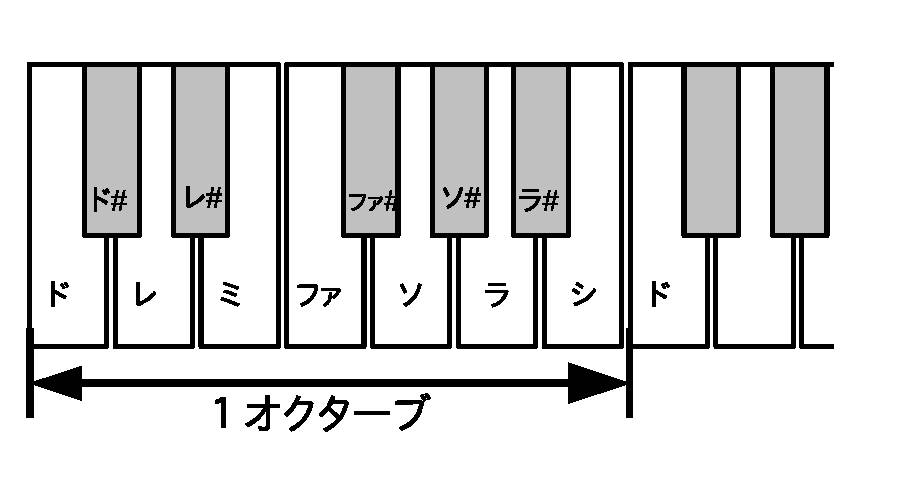
\includegraphics[width=6.2cm]{octave.eps}
    \caption{ピアノの鍵盤}\label{fig:octave}
\end{figure}

さて, 音階を, 周波数が等比数列になるように決めることを, 平均律と呼ぶ。多くの
楽器は平均律で調整されている。以後, 平均律の12音階を考える。
\begin{enumerate}
\item 楽器の調律では, 音階の基準として
周波数440 Hzの「ラ」の音が使われる。この音の2オクターブ上のラ音の
周波数はどのくらいか?
\item 12音階の周波数を等比数列とみたときの公比はどのくらいか?
\item 多くのピアノは, 88個の鍵を持つ。つまり, 88個の音階を出せる。そのような
ピアノの最高音の周波数は, 最低音の周波数の何倍か?
\item 人間耳は, 概ね20Hzから20000Hzまでの音を感じる。その
範囲は何オクターブに相当するか?
\item 上記の範囲をカバーするピアノを作るとしたら, 鍵はいくつ必要か?
\item 基準の「ラ」の音(周波数440 Hz)の, 1.5倍の周波数を持つ音は, 12音階の
中で, どの音階になるか?
\item 1オクターブの中で, ド, ミ, ソのそれぞれの周波数は, およそ4:5:6という
整数比に近い比になることを示せ(これが, ドミソが綺麗な和音になる理由)。
\end{enumerate}
\end{exq}

\begin{exq}\label{q:paper_reflectance} 反射率$r$, 透過率$t$の紙がある。
\begin{enumerate}
\item この紙を2枚かさねたときの反射率を$r$と$t$で表せ。
ヒント: 2枚の紙を, 上から「紙1」「紙2」とする。この2枚重ねの紙に当たった光のうち, 「反射」されるのは, 
\begin{itemize}
\item 紙1の表面で反射される成分。
\item 紙1を透過して紙2の表面で反射し, 紙1を透過する成分。
\item 紙1を透過して紙2の表面で反射し, 紙1の裏面で反射し, 紙2の表面で反射し, 紙1を透過する成分。
\item ...
\end{itemize}
の総和である。
\item 反射率80%, 透過率15%の紙を2枚重ねた時の反射率を求めよ。
\end{enumerate}
\end{exq}

\section*{問題の解答}

\noindent{\textbf{答}}\ref{q:alg_ineq4}  
与式は両辺とも0以上なので, \eref{eq:th_order_9}より, \\左辺$^2 \geq$右辺$^2$を言えばよい。
\begin{eqnarray*} 
&&(\text{左辺})^2-(\text{右辺})^2=\frac{a^2+2ab+b^2}{4}-ab\\
&&=\frac{a^2-2ab+b^2}{4}=\Bigl(\frac{a-b}{2}\Bigr)^2\ge0
\end{eqnarray*}
よって与式は成り立つ。この式で, 等号が成り立つときは$\{(a-b)/2\}^2=0$
なのだから, $(a-b)^2=0$。\eref{eq:ab_0_a_0_b_0}より, $a-b=0$。従って$a=b$。\qed
\mv

\noindent{\textbf{答}}\ref{q:alg_prod0} (1) $4 \cdot 3 \cdot 2 \cdot 1 = 24$  
(2) $5 \cdot 4 \cdot 3 \cdot 2 \cdot 1 = 120$  (3) $1$  (4) $1$  (5) 存在しない。\mv

\noindent{\textbf{答}}\ref{q:alg_comb5} $5!=120$ 通り。
\mv

\noindent{\textbf{答}}\ref{q:alg_comb00} \eref{eq:junretsu}において, $m=n$とすれば, \\
$_n\text{P}_n = n!/(n-n)!=n!/0!=n!$\qed
\mv

\noindent{\textbf{答}}\ref{q:alg_comb0} 8人から3人を選んで順に並べ, その順番で会長・副会長・会計係を割り当てればよい。
つまり, 8人から3人を選ぶ順列だから, $_{8}{\text P}_3 = 336$ 通り。
\mv


\noindent{\textbf{答}}\ref{q:alg_01_8} $2^8=256$通り。
\mv

%\noindent{\textbf{答}}\ref{q:alg_comb2}  
%与式の左辺は, \eref{eq:combination}で$n, m$をそれぞれ$n+1, m+1$とすれば,
%\begin{eqnarray}
%_{n+1}{\text C}_{m+1} & = & \frac{(n+1)!}{(m+1)!\{n+1-(m+1)\}!}\nonumber\\
%                      & = & \frac{(n+1)!}{(m+1)!(n-m)!}\label{eq:sol_alg_comb20}
%\end{eqnarray}
%となる。一方, 与式の右辺第1項は, \eref{eq:combination}で$n, m$をそれぞれ$n, m+1$とすれば, 
%\begin{eqnarray*}
%_{n}{\text C}_{m+1} &=& \frac{n!}{(m+1)!\{n-(m+1)\}!}\\
%                     &=& \frac{n!}{(m+1)!(n-m-1)!}
%\end{eqnarray*}
%となり, 与式の右辺第2項は\eref{eq:combination}をそのまま使えば
%\begin{eqnarray*}
%_{n}{\text C}_{m} =  \frac{n!}{m!(n-m)!}
%\end{eqnarray*}
%となるから, 与式の右辺は, 
%\begin{eqnarray}
%&&_{n}{\text C}_{m+1} +_{n}{\text C}_{m}\nonumber\\
%&& = \frac{n!}{(m+1)!(n-m-1)!} +  \frac{n!}{m!(n-m)!}\nonumber\\
%&& = \frac{n!(n-m)}{(m+1)!(n-m)!}+\frac{n!(m+1)}{(m+1)!(n-m)!}\nonumber\\
%&& = \frac{n!(n-m)+n!(m+1)}{(m+1)!(n-m)!} = \frac{n!(n-m+m+1)}{(m+1)!(n-m)!}\nonumber\\
%&& = \frac{n!(n+1)}{(m+1)!(n-m)!}\nonumber\\
%&& =  \frac{(n+1)!}{(m+1)!(n-m)!}\label{eq:sol_alg_comb21}
%\end{eqnarray}
%となる。\eref{eq:sol_alg_comb20}と\eref{eq:sol_alg_comb21}が等しいから, 
%与式の左辺と右辺は等しい。従って与式が成り立つ\footnote{
%注: この問題は, 以下のように考えることができる。$n+1$人の集団から$m+1$人の
%代表を選ぶとしよう。無論, その選び方は$_{n+1}$C$_{m+1}$通りである。さて, その集団の
%中の特定の一人(ここではAさんと呼ぼう)に着目する。Aさんが代表に入らない場合, 
%その場合の数は, 残り$n$人の中から$m+1$人の代表を選ぶ場合の数になるので, $_n$C$_{m+1}$通り。
%Aさんが代表に入る場合, その場合の数は, 残り$n$人の中から$m$人の代表を選ぶ場合の数になる
%ので, $_n$C$_m$通り。この2パターンで全ての場合を網羅するので, 結局, 与式が成り立つ。}。
%\mv


\noindent{\textbf{答}}\ref{q:alg_comb3} 
(1) 4 (2) 10 (3) 10\\
(4) $n(n-1)(n-2)/6$\\
(5) $_{n}{\text C}_{0}=n!/(0!n!)=n!/n!=1$。ここで$0!=1$を使った。 
(6) 1
\mv

\noindent{\textbf{答}}\ref{q:alg_comb1} 
\eref{eq:combination}より, 
\begin{eqnarray*}
_n{\text C}_m = \frac{n!}{m!\,(n-m)!}
\end{eqnarray*}
一方, \eref{eq:combination}で$m$を$n-m$と置き換えれば, 
\begin{eqnarray*}
_n{\text C}_{n-m} & = & \frac{n!}{(n-m)!\,\{n-(n-m)\}!}\\
                  & = & \frac{n!}{(n-m)!m!} = \frac{n!}{m!(n-m)!}
\end{eqnarray*}
よって, $_n{\text C}_m\,=\,_n{\text C}_{n-m}$ \qed
\mv

\noindent{\textbf{答}}\ref{q:alg_comb4} $_{40}{\text C}_3 = 9880$ 通り。
\mv

\begin{comment}
\noindent{\textbf{答}}\ref{q:alg_poly_tenkai0} 
\begin{edaenumerate}
\item $a^2 + 2ab + b^2$
%\item $a^2 - 2ab +b^2$
%\item $a^3 +3 a^{2} b + 3 a b^{2} + b^3$
\item $a^3 -3 a^{2} b + 3 a b^{2} - b^3$
%\item $a^2 - b^2$
\item $a^3 - b^3$
%\item $a^3 + b^3$
\item $2x^3 + 5x^2 - x - 6$
\end{edaenumerate}
(5) $a^2 + b^2 + c^2 + 2ab + 2bc + 2ca$
\mv
\end{comment}


\noindent{\textbf{答}}\ref{q:alg_poly_tenkai01} $\,\,\,2x^3+3x^2\chi-3x\chi^2-2\chi^3$
\mv

\noindent{\textbf{答}}\ref{q:alg_poly_tenkai2} (1) \eref{eq:binomth}で$a=x$, $b=1$, $n=7$とすれば, 
$(x+1)^7\,=\,_7\text{C}_7\,x^7\,+\,_7\text{C}_6\,x^6\,+\,_7\text{C}_5\,x^5\cdots$
となる。$x^3$の項は, $_7\text{C}_3x^3=35x^3$。従って, 35。 (2) \eref{eq:binomth}で$a=2x$, $b=-3$, $n=6$とすれば, $x^3$の項は
$_6\text{C}_3(2x)^3\times(-3)^3=-4320x^3$。従って, $-4320$。\mv

\begin{comment}
\noindent{\textbf{答}}\ref{q:alg_insu0}  
\begin{edaenumerate}
\item $(a+b)^2$
\item $(a-b)^2$
\item $(a+b)(a^2 - ab + b^2)$
\item $(a-b)(a^2 + ab + b^2)$
\item $(a^2 + b^2)(a+b)(a-b)$
\item $(x-2)(x+1)$
\item $(2x+1)(x-3)$
\item $x(x-1)(x+1)$
\end{edaenumerate}
(9) $x^2=X$とおくと, 与式は,
\begin{eqnarray*}
X^2-5X+4&=&(X-1)(X-4)\\
        &=&(x^2-1)(x^2-4)\\
        &=&(x+1)(x-1)(x+2)(x-2)
\end{eqnarray*}

\noindent{\textbf{答}}\ref{q:alg_wari0}  
\begin{enumerate}
\item 
\begin{eqnarray*}\izyohou{1,1,-1,1}{1,-1}\end{eqnarray*}
従って, 商$x^2 + 2x + 1$,余り$2$
\item 
\begin{eqnarray*}\izyohou{1,2,-1,2,-1}{1,1,1}\end{eqnarray*}
従って, 商$x^2 + x -3$,余り$4x+2$
\end{enumerate}
\hv


\noindent{\textbf{答}}\ref{q:alg_insu3}  
\begin{edaenumerate}
\item $(x-1)(x+2)(x+3)$
\item $(x+1)(x-2)(x+4)$
\end{edaenumerate}
\hv
\end{comment}

\noindent{\textbf{答}}\ref{q:alg_heihokansei0} 
\begin{edaenumerate}<3>
\item \begin{eqnarray*}(x + 2)^2 + 1\end{eqnarray*}
\item \begin{eqnarray*}\Bigl(x + \frac{1}{2}\Bigr)^2 + \frac{3}{4}\end{eqnarray*}
\item \begin{eqnarray*}(x - 1)^2 - 2\end{eqnarray*}
\item \begin{eqnarray*}2(x+1)^2 + 1\end{eqnarray*}
\item \begin{eqnarray*}4\Bigl(x+\frac{1}{8}\Bigr)^2 + \frac{15}{16}\end{eqnarray*}
\end{edaenumerate}
\mv


\noindent{\textbf{答}}\ref{q:alg_eq_insu0} 略解 (レポートではきちんと導出過程を書こう):
(1) $x=-2,3$  (2) $x=1,2$  (3) 左辺を因数分解すると, $(x^2-4)(x^2-1)=(x+2)(x-2)(x+1)(x-1)$。
従って, $x=\pm1, \pm2$
\mv


%\noindent{\textbf{答}}\ref{q:alg_2eq0} 略(誘導に従って計算する。)
%\mv


\noindent{\textbf{答}}\ref{q:alg_eq_complex0} 略解(レポートではきちんと導出過程を書こう):
(1) $x=(-1 \pm \sqrt{7}\,i)/2$ (2) $x=(-3 \pm \sqrt{5})/2$
%\item $x=-1,\, (-1 \pm \sqrt{7}\,i)/2$
%\item $x=1,\, (-1 \pm \sqrt{3}\,i)/2$
%\item $x=\pm 1,\, \pm\, i$
\mv


\noindent{\textbf{答}}\ref{q:alg_series0} (1) $2n -1$ (2) $11 -n$ 
(3) $3^n$ (4) $(1/2)^{n-1}$\mv


% 以下の実数列は, 単調増加するか, 単調減少するか, それともどちらでもないか, 述べよ。
\noindent{\textbf{答}}\ref{q:alg_series1} 
\begin{enumerate}
\item 単調増加。例: $\{1,2,3,4,\cdots\}$
\item 単調減少。例: $\{4,3,2,1,\cdots\}$
\item 単調増加。例: $\{1,2,4,8,\cdots\}$
\item 単調減少。例: $\{-1,-2,-4,-8,\cdots\}$
\item どちらでもない。例: $\{1,-2,4,-8,\cdots\}$
\item 単調減少。例: $\{1,1/2,1/4,1/8,\cdots\}$
\item 単調減少。
\end{enumerate}
\mv


% 以下の実数列は, 収束するか, 発散するか? 収束するならどういう値に収束するか?
\noindent{\textbf{答}}\ref{q:alg_series3} 
\begin{edaenumerate}
<3>
\item 発散($\infty$)
\item 発散($-\infty$)
\item 発散($\infty$)
\item 発散($-\infty$)
\item 0に収束
\item 0に収束
\item 0に収束
\end{edaenumerate}
\mv


\noindent{\textbf{答}}\ref{q:alg_series_sum0} 
\begin{edaenumerate}
\item $2+2+2+2=8$
\item $1+4+9=14$
\item $1+2+4+8=15$
\item $3+5+7+9=24$
\end{edaenumerate}
\mv

\noindent{\textbf{答}}\ref{q:sum_binomth2} 
\begin{eqnarray}
(a+b)^n=\sum_{k=0}^n \,_n\text{C}_k\,a^{n-k}\,b^k
\end{eqnarray}

%\noindent{\textbf{答}}\ref{q:alg_induction_freqmiss} (解答例)\eref{eq:sumk_1}はあくまで$N$で成り立つことを仮定しているだけで, それが$N+1$で成り立つ保証はない。ていうか, それを示すのがそもそもの目的。君は, 示すべき式自体を根拠にしてしまっている。\mv

\noindent{\textbf{答}}\ref{q:alg_series_sum1} 
\begin{enumerate}
\item $n=1$のとき, 与式は, 左辺=$1+r$, 右辺=$1+r$
となるので成り立つ。$n=N$のとき与式が成り立つと仮定する。すなわち, 
\begin{eqnarray}
\sum_{k=0}^N r^k=\frac{1-r^{N+1}}{1-r}\label{eq:sum_touhi_ans2}
\end{eqnarray}
と仮定する。そのとき, 
\begin{eqnarray*}
\sum_{k=0}^{N+1} r^k=\sum_{k=0}^{N} r^k+r^{N+1}=\frac{1-r^{N+1}}{1-r}+r^{N+1}\\
= \frac{1-r^{N+1}+r^{N+1}-r^{N+2}}{1-r} = \frac{1-r^{N+2}}{1-r}
\end{eqnarray*}
となり, $n=N+1$についても与式は成り立つ。\qed
\item $n=1$のとき, 与式は, 左辺=1, 右辺=1となるので成り立つ。
$n=N$のとき与式が成り立つと仮定する。すなわち, 
\begin{eqnarray*}
\sum_{k=1}^N k^2=\frac{N(N+1)(2N+1)}{6}
\end{eqnarray*}
と仮定する。そのとき, 
\begin{eqnarray*}
\sum_{k=1}^{N+1} k^2 & = & \sum_{k=1}^{N} k^2+(N+1)^2\\
        & = & \frac{N(N+1)(2N+1)}{6}+(N+1)^2\\
        & = & \frac{(N+1)\{N(2N+1)+6(N+1)\}}{6}\\
        & = & \frac{(N+1)(2N^2+7N+6)}{6}\\
        & = & \frac{(N+1)(N+2)(2N+3)}{6}
\end{eqnarray*}
これは\eref{eq:sum_xsquare}の右辺で$n$を$N+1$としたものに等しい。従って
与式は$n=N+1$についても成立。
\end{enumerate}

\noindent{\textbf{答}}\ref{q:alg_sum2} 
(1) \eref{eq:sum_touhi}より, $(1-2^{11})/(1-2)=2047$ 
(2) \eref{eq:sum_xsquare}より, $(10\times11\times21)/6=385$

% パソコンの表計算ソフトで, 以下の数列の和を適当に大きな$n$について計算せよ:
%\noindent{\textbf{答}}\ref{q:comp_sum1}  略。

\include{03_algebra_ans}
\chapter{関数}\label{chapt_function}

%知るを知るとし, 知らざるを知らずとす。これ知るなり(孔子)。\hv

\section{関数のグラフ}

\underline{関数}\index{かんすう@関数} (function)
とは, 何か数を与えると, その数に応じて何か決まった数を返すような, 
対応関係のことである(定義)。例えば関数$y=x^2$は, 実数$x$を与えると, 
その2乗を$y$として返す。この場合, $x=3$を与えると, $y=3^2=9$を返す
\footnote{関数は, この例のように, 数式で表される
ことも多いが, 数式で表すことのできない関数もある。数を
与えるとそれに応じて決まった数を返す, という対応関係が
はっきりしていれば, 必ずしもその対応関係が数式で表されなくてもよいのだ。}。

関数を語るときの一般論の中では, 関数を$y=f(x)$と表すことが多い
(上の例では$f(x)$は$x^2$である)。別に$f$でなくても$a(x)$で
も$b(x)$でも何でもいいのだが, とりあえずfunctionの頭文字を
とって$f$をよく使う。

$x$に何かの値を与えると, $y=f(x)$から$y$の値が求められる。
このとき, 与えられる数(この場合は$x$)を\underline{独立変数} 
\index{どくりつへんすう@独立変数}
%(independent variable)
もしくは引数(ひきすう)\index{ひきすう@引数}といい, 求められる数(この場合は$y$)
を\underline{従属変数} \index{じゅうぞくへんすう@従属変数}
%(dependent variable)
という(定義)。

いろんな自然現象や社会現象は関数で表現され, 関数で予測される。
そのための数学, つまり関数を取り扱う数学を
「解析学\index{かいせきがく@解析学}」という。解析学の第一歩は, 
いろんな関数を適切にグラフに描くことである。

なお, この章では, 出てくる数は全て実数とする (複素数を扱う関数も存在するが, 
この章では考えない)。

さて, 最も単純な関数は「定数関数」\index{ていすうかんすう@定数関数}だ。
定数関数とは, 独立変数がどのような値であっても, 従属変数の値が
いつも同じ定数であるような関数である(定義)。
\begin{exmpl} 
\begin{eqnarray}y=1\label{eq:ex_constfunc1}\end{eqnarray}
は定数関数だ。式に$x$が入っていないから, $x$がどんな値を取ろうが無関係に, 
$y$の値は1。グラフは図\ref{fig:const}のように$x$軸に平行な直線になる。
(例おわり)
\begin{figure}[h]
    \centering
    \includegraphics[width=5cm]{const.eps}
    \caption{定数関数 $y=1$のグラフ。}\label{fig:const}
\end{figure}\end{exmpl}\mv
\begin{freqmiss}{\small\textgt{グラフに原点O, $x$軸の先の$x$, $y$軸の先の$y$等の記入を忘れる}
... グラフには, 原点(O), $x$軸(矢印と$x$), $y$軸(矢印と$y$)を必ず描き込むこと。}\end{freqmiss}

さて, 次に単純なのは, 中学校で習った
\begin{eqnarray}y=2x\label{eq:ex_propfunc2}\end{eqnarray}
のような関数だ。$y=2x$は, $x=0, 1, 2, \cdots$のときに, それぞれ
$y=0, 2, 4, \cdots$のような値をとる。グラフは図\ref{fig:proportion}の左側の
ように, 原点を通る, 右上がりの直線だ。一方, $y=-2x$のような関数のグラフは, 
図\ref{fig:proportion}の右側のように, 原点を通る, 右下がりの直線になる。
\begin{figure}[h]
    \centering
    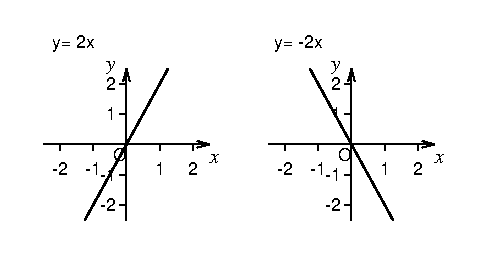
\includegraphics[width=8.5cm]{proportion.eps}
    \caption{比例関係 $y=2x$と$y=-2x$のグラフ}\label{fig:proportion}
\end{figure}

一般に, $a$を定数として, 
\begin{eqnarray}y=ax\label{eq:ex_propfunc22}\end{eqnarray}
という関数のグラフは, 原点を通る直線になる。定数$a$が正なら右上がり, 
負なら右下がりの直線だ。$a$が正のとき, $a$が大きいほど, $x$が増えるに
つれて$y$は急に増加するので, 直線は急になる。もっと言えば, 
この定数$a$は, 「$x$方向に1増えると$y$方向にいくつ増えるか」
を表す。この定数$a$のことを, 直線の\underline{傾き} \index{かたむき@傾き}と呼ぶ。

このように, $y=ax$のような関数で対応付けられる$x$と$y$の関係を, 
比例関係\index{ひれいかんけい@比例関係}とか「$y$と$x$は比例する」
と言う(定義)\footnote{$y=ax$は比例関係だが, $y=ax+1$は
比例関係ではない。グラフで描くと, 原点を通る直線関係だけが比例関係。}。
$x$と$y$が比例するということを, $x \propto y$とか$y \propto x$と書いたりもする。\hv

次に, 関数
\begin{eqnarray}y=x^2\label{eq:exxsq}\end{eqnarray}
を考えよう。これは, $x=0, 1, 2, 3, \cdots$のときに, 
それぞれ$y=0, 1, 4, 9, \cdots$をとる。グラフは図\ref{fig:parab_inverse}
左のようになる。こういう形のグラフや, それを引き伸ばしたり回転したグラフを
「放物線」\index{ほうぶつせん@放物線}という。

%\begin{figure}[h]
%    \centering
%    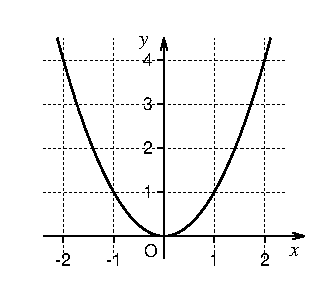
\includegraphics[width=6.0cm]{parab.eps}
%    \caption{放物線 $y=x^2$のグラフ}\label{fig:parab}   
%\end{figure}

\begin{figure}[h]
    \centering
    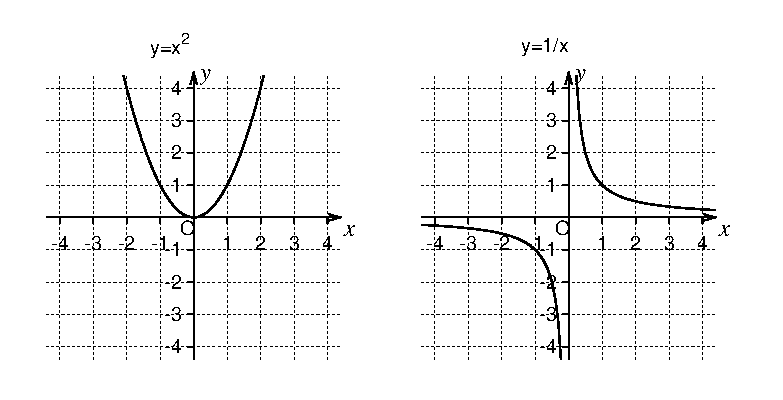
\includegraphics[width=8.3cm]{parab_inverse.eps}
    \caption{左: 放物線$y=x^2$, 右: 双曲線$y=1/x$}\label{fig:parab_inverse}
\end{figure}

次に, 関数
\begin{eqnarray}y=\frac{1}{x}\label{eq:ex1ovsrx}\end{eqnarray}
を考えよう。「0での割り算」は許されないから, この関数は$x=0$
のときに値を持たない。また, 例えば$x=1/2, 1, 2$のときに, それぞれ$y=2, 1, 1/2$という
値をとる。グラフは図\ref{fig:parab_inverse}右のようになる。

%\begin{figure}[h]
%    \centering
%    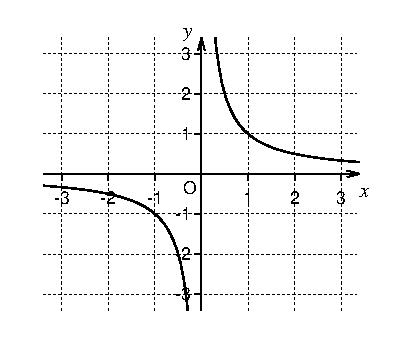
\includegraphics[width=7cm]{inverse.eps}
%    \caption{双曲線(反比例関係) $y=1/x$のグラフ}\label{fig:inverse}
%\end{figure}

\eref{eq:ex1ovsrx}の関数は, $x$がどんどん大きくなると(グラフの右にどんどん行くと), 
限りなく0に近づく(グラフの線は$x$軸に近づく)。そのようなことを, 「$x$が無限大に行く極限では, 
$1/x$は0に収束する」と言ったり, 
\begin{eqnarray}
x\rightarrow \infty \text{のとき, }\frac{1}{x}\rightarrow0
\end{eqnarray}
と書く。あるいは, 
\begin{eqnarray}
\lim_{x\rightarrow \infty}\frac{1}{x}=0\label{eq:limit_new}
\end{eqnarray}
という式であらわす。このlimはリミットと読み, 「\underline{極限}」\index{きょくげん@極限}
を意味する。極限とは, 何かを特定の状況に限りなく近づけていくことだ。limの下にその
状況を記す約束である。この場合は$x\rightarrow \infty$がそれにあたる。

このグラフ(図\ref{fig:parab_inverse}右)は, $x$軸と$y$軸に対して, 交わったり
接したりすることはないが, 限りなく接近する。そのような直線(この場合は$x$軸と$y$軸)
を\underline{漸近線} (ぜんきんせん)\index{ぜんきんせん@漸近線}
% (asymptote)
という。

一般に, $a$を定数として, 
\begin{eqnarray}y=\frac{a}{x}\label{eq:ex1ovsrx2}\end{eqnarray}
のような関数による$x$と$y$の関係を, 「反比例関係」\index{はんぴれいかんけい
@反比例関係}とか「$y$と$x$は反比例する」と言う(定義)。また, こういう形のグラフや, 
それを引き伸ばしたり回転させたりしたグラフを「双曲線」\index{そうきょくせん@双曲線}という。\hv

%2011.07.07 山崎 微修正。ここ以降で「べき関数」という単語がことわりなしに出てくるので, ここで定義した。
以上の関数(\eref{eq:ex_constfunc1}$\sim$\eref{eq:ex1ovsrx}, \eref{eq:ex1ovsrx2})は, 
$a$を定数, $n$を整数として, 次式のように統一的に書ける:
\begin{eqnarray}
y=ax^n\label{eq:func_power_func}
\end{eqnarray}
こういう関数をまとめて\underline{べき関数}\index{べきかんすう@べき関数}と呼ぶ。
ここまで学んだ事をまとめると, 「べき関数(\eref{eq:func_power_func})のグラフは,  
\begin{itemize}
\item $n=0$のときには直線(定数関数)
\item $n=1$のときには直線(比例関係)
\item $n=2$のときには放物線
\item $n=-1$のときには双曲線(反比例関係)
\end{itemize}
になる」とも言える。べき関数とそのグラフをきっちり理解すれば, 
他のいろんな関数も扱いやすくなる。\hv

\section{平行移動・拡大縮小・対称移動}\label{sec:func_trans}

一見, 複雑な関数のグラフも, より単純な関数のグラフを移動したり
変形したものとみなせることが多い。ここではその基礎となる考え方を学ぼう。

まず, 例として$xy$平面上の点$(2,3)$を考える。この点を, 
横($x$軸の正の方向)に1だけ移動したら, その座標は$(3,3)$になる。また, 
この点を縦($y$軸の正の方向)に2移動したら, その座標は$(2, 5)$に
なる(実際に$xy$平面を描いて確認せよ)。

\begin{q}\label{q:func_trans0} この点$(2, 3)$について, 以下が成り立つことを, 
実際に$xy$平面を描いて確認せよ。
\begin{enumerate}
\item $x$軸の正方向に5移動した点の座標は$(7, 3)$
\item $y$軸の正方向に4移動した点の座標は$(2, 7)$
\item $x$軸方向に3倍拡大した点の座標は$(6, 3)$
\item $y$軸方向に1/2倍拡大した点の座標は$(2, 3/2)$
\item $x$軸に関して対称\footnote{$x$軸に関して対称という
ときの「対称」を, 高校までは「線対称」と呼んだりした。
しかし, $x$軸はそもそも線だから, それに関して
対称ということが線対称を意味するのは自明。だから, 
「線対称」という言葉は使わない。同様に, 下の「原点に関して
対称」という「対称」は高校までの「点対称」を意味するのは明らかだろう。}
に移動した点の座標は$(2, -3)$
\item $y$軸に関して対称に移動した点の座標は$(-2, 3)$
\item 原点に関して対称に移動した点の座標は$(-2, -3)$
\end{enumerate}\end{q}
\mv

一般に, $xy$座標平面上の点$(x_0, y_0)$について, 
\begin{itemize}
\item $x$軸の正方向に$a$移動した点の座標は$(x_0+a, y_0)$
\item $y$軸の正方向に$a$移動した点の座標は$(x_0, y_0+a)$
\item $x$軸方向に$a$倍した点の座標は$(ax_0, y_0)$
\item $y$軸方向に$a$倍した点の座標は$(x_0, ay_0)$
\item $x$軸に関して対称に移動した点の座標は$(x_0, -y_0)$
\item $y$軸に関して対称に移動した点の座標は$(-x_0, y_0)$
\item 原点に関して対称に移動した点の座標は$(-x_0, -y_0)$
\end{itemize}
だ。これらは問\ref{q:func_trans0}の経験から直感的にわかるだろう。\hv

一般に, 関数
\begin{eqnarray}y=f(x)\label{eq:y_fx}\end{eqnarray}のグラフを, 
$x$軸の正方向に$a$, $y$軸の正方向に$b$だけ平行移動\index{へいこういどう@平行移動}すると, 
関数
\begin{eqnarray}
y=f(x-a)+b\label{eq:y_fxab}
\end{eqnarray}
のグラフになる。なぜか? $y=f(x)$の上の任意の点Pを考えよう。点Pの座標を
$(x_0, y_0)$とする。点Pは\eref{eq:y_fx}のグラフ上にあるので
\begin{eqnarray}
y_0=f(x_0)\label{eq:y0x0}
\end{eqnarray}
だ。点Pを$x$軸の正方向に$a$, $y$軸の正方向に$b$だけ平行移動した先の点, つまり
点$(x_0+a, y_0+b)$を, 改めて点P$_1$とし, その座標を$(x_1, y_1)$としよう。
すなわち, 
\begin{eqnarray}
x_1=x_0+a\\
y_1=y_0+b
\end{eqnarray}
である。すなわち, $x_0=x_1-a,\, y_0=y_1-b$である。これを\eref{eq:y0x0}に代入すると, 
\begin{eqnarray}
y_1-b=f(x_1-a)\label{eq:y_fxab4}
\end{eqnarray}
すなわち, 
\begin{eqnarray}
y_1=f(x_1-a)+b
\end{eqnarray}
となる。従って, $(x_1, y_1)$, つまり点P$_1$は\eref{eq:y_fxab}のグラフの上にある。\qed

\begin{faq}{\small\textgt{\eref{eq:y_fxab}がしっくり来ません。$a$と$b$の前の
符号が違うのが気持ち悪いのです。$y=f(x-a)-b$とか$y=f(x+a)+b$にならないのは
なぜですか?} ... \eref{eq:y_fxab}を, $y-b=f(x-a)$と書き直したら
$a$と$b$は同じ符号で現れるでしょ? \eref{eq:y_fxab}はもともとこういう
形だったのです(\eref{eq:y_fxab4}をチェック!)。}\end{faq}

一般に, 関数$y=f(x)$のグラフに関して, 以下の定理が成り立つ:\\
定理1) $x$軸の正方向に$a$, $y$軸の正方向に$b$だけ平行移動すると, $y=f(x-a)+b$のグラフになる。\\
定理2) $x$軸方向に$a$倍すると, $y=f(x/a)$のグラフになる。\\
定理3) $y$軸方向に$a$倍すると, $y=af(x)$のグラフになる。\\ 
定理4) $x$軸に関して対称移動\index{たいしょういどう@対称移動}すると, $y=-f(x)$のグラフになる。\\
定理5) $y$軸に関して対称移動すると, $y=f(-x)$のグラフになる。\\
定理6) 原点に関して対称移動すると, $y=-f(-x)$のグラフになる。\mv

上では定理1を証明した。他の定理も同様に証明できる。

\begin{q}\label{q:func_trans1} 上の定理2と定理4を証明せよ。\end{q}
\mv

これらの定理を使って, 先に見た, 直線, 放物線, 双曲線のグラフを元に, 
多様な関数のグラフを表現しよう。
\begin{exmpl}関数
\begin{eqnarray}y=2x-1\label{eq:func_exm_line2x_1}\end{eqnarray}
のグラフ(図\ref{fig:basic_graph}左上)は, 比例関係の関数$y=2x$のグラフを, 
$y$軸の正方向に$-1$だけ(グラフの下方向に1だけ)平行移動したものだ(定理1)。
\end{exmpl}

\begin{exmpl}関数$y=x^2/4$のグラフ(図\ref{fig:basic_graph}右上)は
$y=x^2$のグラフを$y$軸方向に$1/4$倍したもの(定理3)。あるいは, $y=(x/2)^2$とも
書けるから, そのグラフは$y=x^2$のグラフを$x$軸方向に$2$倍したものでもある(定理2)。
\end{exmpl}

\begin{exmpl}関数$y=-x^2$のグラフ(図\ref{fig:basic_graph}左中)は, 
$y=x^2$のグラフを$x$軸に関して対称移動したものだ(定理4)。
\end{exmpl}

\begin{exmpl}関数
\begin{eqnarray}y=2x^2+4x+1\end{eqnarray}
は, 平方完成すると$y=2(x+1)^2-1$
になるから, そのグラフ(図\ref{fig:basic_graph}右中)は, $y=x^2$のグラフを
まず$y$軸方向に2倍して($y=2x^2$), さらに$x$軸の正方向に$-1$, $y$軸の
正方向に$-1$だけ移動したものだ(定理3, 定理1)。
\end{exmpl}

\begin{exmpl}関数$y=-1/x$のグラフ(図\ref{fig:basic_graph}左下)は, $y=1/x$
のグラフを$x$軸に関して対称移動したものだ(定理4)。あるいは$y$軸に関して
対称移動したものとも言える(定理5)。
\end{exmpl}

\begin{exmpl}関数
\begin{eqnarray}y=\frac{x+1}{x-1}\end{eqnarray}
のグラフは? この式を変形すると, 
\begin{eqnarray}y=\frac{x-1+2}{x-1}=1+\frac{2}{x-1}\end{eqnarray}
となる。これは$y=1/x$のグラフを$y$軸方向に2倍し, 
$x$軸の正方向に1, $y$軸の正方向に1だけ移動したものだ(定理3, 定理1)。
それに伴って漸近線も平行移動することに注意! 結果は図\ref{fig:basic_graph}右下。 (例おわり)
\end{exmpl}\mv

\begin{figure}[h]
    \centering
    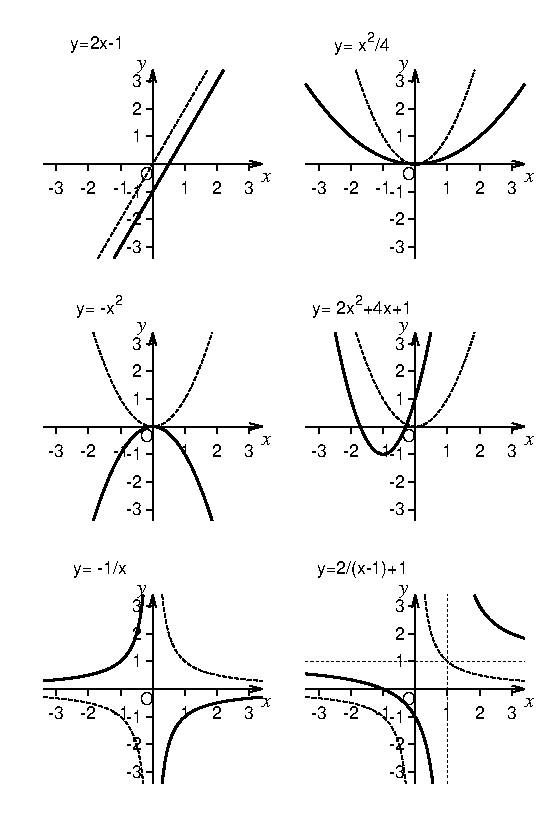
\includegraphics[width=8.2cm]{basic_graph.eps}
    \caption{直線・放物線・双曲線を平行移動・拡大縮小・対称移動することで得られるグラフ。太い点線は, 元になった関数のグラフ。細い点線は漸近線。}\label{fig:basic_graph}
\end{figure}

\begin{q}\label{q:func_trans2} 関数$y=x^2$を以下のように移動や拡大した関数を表す式を, それぞれ書け。
\begin{enumerate}
\item $x$軸の正方向に1, $y$軸の正方向に2だけ平行移動
\item $x$軸方向に2倍, $y$軸方向に3倍だけ拡大
\item $x$軸方向に2倍に拡大し, $x$軸の正方向に1だけ平行移動
\item $x$軸の正方向に1だけ平行移動し, $x$軸方向に2倍に拡大(前問と順序が違うことに注意!)
\end{enumerate}\end{q}
\mv

\begin{q}\label{q:func_trans3} 次の関数のグラフを描け。漸近線がある場合は, その式とグラフも描き込め。
\begin{edaenumerate}
\item $y=2x+1$
\item $y=x^2+2x+3$ 
\item \begin{eqnarray*}y=2+\frac{1}{x}\end{eqnarray*}
\item \begin{eqnarray*}y=\frac{2x}{1+x}\end{eqnarray*}
\end{edaenumerate}\end{q}
\hv



\section{一次関数と直線のグラフ}

$a, b$を実数の定数として(ただし$a\ne0$とする), 
\begin{eqnarray}
y=ax+b\label{eq:y_ax_plus_b0}
\end{eqnarray}
のような関数を, \underline{一次関数} \index{いちじかんすう@一次関数}という。
$y$が$x$の一次式で表されるからだ。例えば\eref{eq:func_exm_line2x_1}は
一次関数である。一次関数は中学高校でやらされて「もう飽きた」という
感じだろう。でも一次関数は, 今後学ぶ, 微分積分や線型代数という数学の
基礎なので, ここで再度, 復習しよう。

\eref{eq:y_ax_plus_b0}のグラフは, $y=ax$のグラフ(直線)を$y$軸の正方向
に$b$移動したものなので直線だ。$x=0$のとき$y=b$だからこのグラフは$(0, b)$で$y$軸
と交わる。この点のことやその$y$座標($b$の値)を\underline{切片}\index{せっぺん@切片}
という。また, $x$が1増えると$y$がいくつ増えるかを表す定数$a$を, \underline{傾き}
という。切片と傾きが定まれば, 一次関数は定まる。

では, 点$(x_0, y_0)$を通り, 傾き$a$の直線の関数は? 平行移動を
使って考えよう。まず, 原点Oを通り傾き$a$の直線の関数は$y=ax$。
これを$x$方向に$x_0$, $y$方向に$y_0$移動すると, \eref{eq:y_fxab}より
次式になる:
\begin{eqnarray}
y=a(x-x_0)+y_0\label{eq:lineeq}
\end{eqnarray}
これが求める関数だ。なぜか? 右辺の$x$に$x_0$を代入したら$y=y_0$だ。
つまりこの直線は$(x_0, y_0)$を通る。$x$の係数は$a$だから, 傾きは$a$。
条件を満たしている! これがうまくいったのは, 直線を平行移動した時, もとの直線$y=ax$の上に
あった原点$(0, 0)$が, 点$(x_0, y_0)$に移動したからである。

では, 2つの点: $(x_0, y_0)$と$(x_1, y_1)$を通る直線の関数は? 
まず, 傾きを求める。点$(x_0, y_0)$から点$(x_1, y_1)$への値
の変化を考えると, $x$軸の正方向に$x_1-x_0$行くと$y$は$y_1-y_0$
だけ増える。従って傾きは$(y_1-y_0)/(x_1-x_0)$。
これを\eref{eq:lineeq}の$a$に代入して得られる次式が, 欲しかった関数である。
\begin{eqnarray}
y=\frac{y_1-y_0}{x_1-x_0}(x-x_0)+y_0\label{eq:lineeq2p}
\end{eqnarray}


\begin{q}\label{q:func_line0} 以下のグラフを表す関数をそれぞれ求めよ。
\begin{enumerate}
\item 傾き$3$, 切片$-2$の直線。
\item 傾き$2$で, 点$(-1,1)$を通る直線。
\item 点$(2,1)$と点$(4,-3)$を通る直線。
\end{enumerate}\end{q}\mv

\begin{q}\label{q:Fahrenheit} 温度を表す単位として, 華氏というものがある
(これは米国で日常的に使われている単位である)。
「華氏$x$度」のことを, $x\,{}^\circ\mathrm{F}$と書く。華氏の定義は以下の
とおりである:
\begin{itemize}
\item 真水の凝固点(つまり0~${}^\circ\mathrm{C}$)を32~${}^\circ\mathrm{F}$とする。
\item 真水の沸点(つまり100~${}^\circ\mathrm{C}$)を212~${}^\circ\mathrm{F}$とする。
\item 摂氏と華氏は一次関数で関係付けられる。
\end{itemize}
華氏$x$度のとき, 摂氏は$y$度であるとする。
\begin{enumerate}
\item $y$を$x$の式で表わせ。
\item $x$を$y$の式で表わせ。
\item 37~${}^\circ\mathrm{C}$を${}^\circ\mathrm{F}$で表わせ (人の体温)
\item 0~${}^\circ\mathrm{F}$を${}^\circ\mathrm{C}$で表わせ。\\
(3)(4)の数値は小数第1位まで記せ。
\end{enumerate}
\end{q}
\hv

\section{関数の和のグラフ}

よく知られた関数の和で表される関数のグラフは, それぞれの関数のグラフを積み重ねる
ようにプロットすることで描くことができる。
\begin{exmpl}
次の関数:
\begin{eqnarray}y=x+\frac{1}{x}\end{eqnarray}
のグラフを, $0<x$の範囲で描いてみよう。この関数は$y=x$と$y=1/x$の和だ。それらを
まず描き, 次に, いくつかの$x$の値について, 2つのグラフを積み上げたところに点を
打つ。例えば$x=1$では$y=x$も$y=1/x$も$y=1$なので, 和は2。
従って, この関数のグラフは$(1, 2)$を通るので, $(1, 2)$に点を描く。片方の
グラフをもう片方のグラフの上に載せるイメージである。

$x\rightarrow \infty$では$y=1/x$は0に漸近するので, この関数のグラフ
は$y=x$に漸近する。一方, $x$が$0$に近づくと$y=1/x$が$\infty$, $y=x$が0に行くので, 
この関数のグラフは$\infty$に行く。それらを勘案
すれば, 図\ref{fig:x_plus_1_over_x}のようなグラフが描ける。(例おわり)\end{exmpl}
\begin{figure}[h]
    \centering
    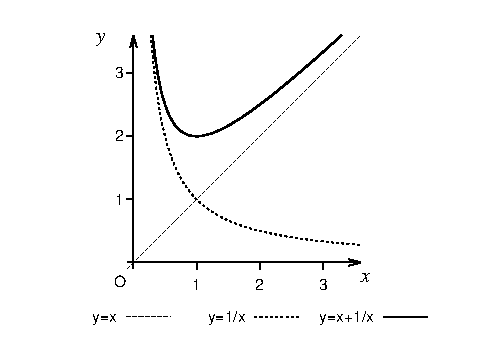
\includegraphics[width=8cm]{x_plus_1_over_x.eps}
    \caption{$y=x+1/x$のグラフ(実線)。$y=x$を土台としてその上に$y=1/x$を
載せるイメージで!}\label{fig:x_plus_1_over_x}
\end{figure}

\begin{q}\label{q:x_plus_1_over_x} 以上の説明をたどって, $y=x+1/x$の
グラフを描け。\end{q}\hv



\section{グラフの読み取りと直線近似}

グラフは, 実験結果を解析したり表示するときにも使う。そういうグラフの
例を図\ref{fig:read_a_graph}に示す。この実験では$x$と$y$の2つの
数値がペアになったデータが得られている。1つのデータペアが1個の点に描かれて
いる。では, 点Aのデータの, $x$と$y$の値はどのくらいだろうか?

\begin{figure}[h]
    \centering
    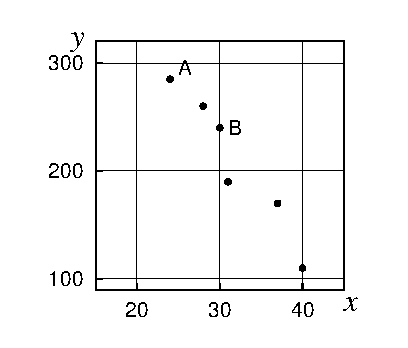
\includegraphics[width=9cm]{read_a_graph.eps}
    \caption{実験値がプロットされたグラフの例}\label{fig:read_a_graph}
\end{figure}

残念なことに, このグラフは目盛りの間隔が広すぎて, ぱっと見ただけでは, 
点Aの$x$の値は20と30の間, $y$の値は200と300の間(で300にかなり近い)
ということしかわからない。正確な数値を得るには, 定規を使う。

まず, 点Aを通る, 縦軸に平行な線を定規で引こう。それが$y=200$の横罫線
と$y=300$の横罫線に交わる点を, それぞれP, Qとする。紙の上での
線分PQの長さ$\overline{\text{PQ}}$と線分PAの長さ$\overline{\text{PA}}$を
それぞれ定規で測ろう(mm単位でもcm単位でもよい)。Aの$y$座標の値は, 
\begin{eqnarray}
\frac{\overline{\text{PA}}}{\overline{\text{PQ}}}\,(300-200)+200
\end{eqnarray}
である(理由は自分で考えてみよう!)。同様に, 点Aを通る, 
横軸に平行な線を定規で引き, $x=20$と$x=30$の縦罫線と交わる点を
求め, 適当な線分の長さを定規で測って上の式と同様の計算すれば, 
$x$座標の値がわかる。\mv

\begin{q}\label{q:read_a_graph} 点Aの$x$座標と$y$座標を実際に
読み取ってみよう! 定規で測った数値を明記し, それらをもとに
計算した式と結果を述べよ。{\small ヒント: 電卓を使ってよい。
結果は, $x=24$, $y=285$程度になるはず。多少の誤差($x$で0.5程度, 
$y$で2程度)は仕方がない。なるべく丁寧に!}\end{q}\mv

\begin{q}\label{q:read_a_graph_line} 図\ref{fig:read_a_graph}の
全ての点に最も近いような1本の直線を, 感覚を頼りに, 定規で引け。
その直線を表す$y=ax+b$という1次式($a$, $b$は適当な定数)を求めよ。
どのように求めたのかわかるように述べよ。{\small ヒント: こういうのを近似直線という。
近似直線をデータから計算で求める方法もあるのだが(最小二乗法と言う), 
紙の上で感覚を頼りに「えいやっ」と引くことも多い。多少の誤差は仕方ない。
直線を定規で引いたら, その傾きと切片を求めればよい。まず, 直線が
罫線と交わる点を利用し, $y$の変化量と$x$の変化量を
それぞれ読み取り, その比を計算する。それが傾き$a$である。
切片は$y$軸との交点だが, このグラフでは$y$軸は載っていない
(左外にある)。そこでかわりに, $y=ax+b$の$(x, y)$に, 問\ref{q:read_a_graph}
で求めた点Aの座標を代入し, $b$を決定する。結果は, $a=-10.6$, $b=550$
くらいになるはず。がんばれ!}
\end{q}
\hv


\section{関数のグラフと, 方程式の解}

いくつかの独立変数$x, y, ...$の関数$f(x, y, ...)$について, 
$f(x, y, ...)=0$という形の式を方程式という(定義)。例えば
P.\pageref{sect:algeb_eq}で学んだ代数方程式は, $f(x, y, ...)$が多項式のときの
方程式である。

\begin{faq}{\small\textgt{\eref{eq:aleq12}で方程式の例として
出てきた$x^2y+xy^2+xy=x+1$は, $f(x)=0$の形をしていませんよ}
... 右辺を左辺に移項して下さい。$x^2y+xy^2+xy-x-1=0$となる
でしょ? この左辺を$f(x, y)$とすると, この式は$f(x, y)=0$の
形になります。}\end{faq}

ここでは独立変数が1個の場合, すなわち$f(x)=0$という形の
方程式を考える。

方程式$f(x)=0$について, $x=x_0$が解なら, $f(x_0)=0$である。
従って, 点$(x_0, 0)$は, 関数$y=f(x)$のグラフ上にある。
すなわち, この点は, 関数のグラフと$x$軸との共有点(交点または
接点)だ。逆に, この関数のグラフと$x$軸との共有点の$x$座標
は, 方程式$f(x)=0$の解だ。これを利用して, いろんな関数の
グラフの概形を描ける。

\begin{exmpl}\label{exmpl:func_xxx_x} 関数$y=x^3-x$の
グラフを描こう。$x^3-x=0$の解は, $x=-1, 0, 1$。
この3つの$x$座標でグラフは$x$軸と交わる(または接する)。
一方, $x\rightarrow\infty$では明らかに$y\rightarrow\infty$, 
$x\rightarrow-\infty$では明らかに$y\rightarrow-\infty$。
つまり大局的には, このグラフは, はるか右上と, はるか左下に
伸びる。以上を総合してえいやっと描けば, 図\ref{fig:xxx-x}
のようなグラフができる。
\begin{figure}[h]
    \centering
    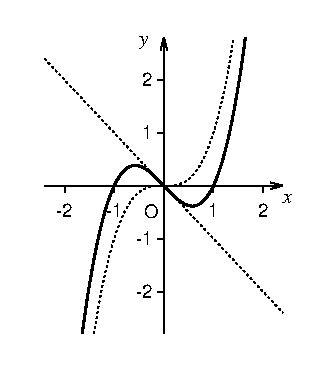
\includegraphics[width=5cm]{xxx-x.eps}
    \caption{$y=x^3-x$のグラフ(実線)。点線は, $y=x^3$と$y=-x$のグラフ。\label{fig:xxx-x}}
\end{figure}

ちなみにこの関数を$y=x^3$と$y=-x$の和とみて, これらの
関数のグラフを積み重ねても描ける。(例おわり)\end{exmpl}\mv

方程式$f(x)=0$の解が実数の範囲で存在しない場合は, $y=f(x)$のグラフは$x$軸と交点を持たない。

\begin{exmpl}$y=x^2+x+1$のグラフを考えよう。方程式$x^2+x+1=0$の
判別式(P.\pageref{eq:Q(uadratic)_E(quations)_D(iscriminant)})は, $D=1-4=-3<0$
である。従ってこの方程式は実数解を持たない(2つの虚数解を持つ)。従って$y=x^2+x+1$のグラフは
$x$軸に接したり交わったりすることはあり得ない。実際, そのグラフは図\ref{fig:2Dpoly_graph}左
のようになる。
(例おわり)\end{exmpl}\mv
\begin{figure}[h]
    \centering
    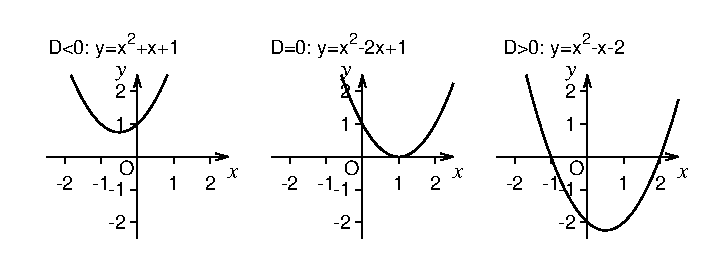
\includegraphics[width=8.3cm]{2Dpoly_graph.eps}
    \caption{2次関数のグラフの例。一般に, 2次関数のグラフは, 判別式$D$の符号によって, 
$x$軸との共有点の様子が決まる。$D<0$なら共有点無し。$D=0$なら共有点(接点)1個。$D>0$なら
共有点(交点)2個。
\label{fig:2Dpoly_graph}}
\end{figure}

$f(x)$が多項式のとき, $f(x)=0$は重解を持つことがある。その場合は, $y=f(x)$のグラフは, 
重解の$x$で$x$軸と接する(その理由は, 後で微分を学べばわかる)。
\begin{exmpl}$y=x^2-2x+1$のグラフを描こう。方程式$x^2-2x+1=(x-1)^2=0$は重解$x=1$を持つ。
従って$y=x^2-2x+1$のグラフは$x=1$で$x$軸に接する。実際, そのグラフは図\ref{fig:2Dpoly_graph}中
のようになる。
(例おわり)\end{exmpl}
\hv

\section{表計算ソフトでグラフを描く}

次に, パソコンで関数のグラフを描いてみよう。原理は簡単で, 関数$y=f(x)$について, 
ある範囲で$x$の値をすこしずつ変えながら, $y$, すなわち$f(x)$を計算し, 点$(x,y)$
をグラフにプロットするだけである。計算は\pref{sect:PC_series}でやった数列の計算と
同じようにやって, グラフ化は表計算ソフトのグラフ機能を使う。\hv

\begin{exmpl}\label{exmpl:graph_y=x^2}
関数$y=x^2$のグラフを$-1\leq x \leq 1$の範囲で描いてみよう(図\ref{fig:PC_graph0})。
左端のA列には, $x$の座標値($-1$から$1$)を適当な間隔(刻み幅という。ここでは0.1)で刻んで(これを離散化という)
入れる。具体的には, セルA2に$-1$を入れ, セルA3には「=A2+0.1」と入れてコピーし, あとはA3をA22までペースト
すればよい。

次に, $x$のそれぞれの値に対応する$y$の値を求める。B2に「=A2*A2」と入れてコピーし, 
B3からB22までペーストすればよい。これで計算が終わった。

最後にグラフを描こう。\underline{A1から}B22まで(A2からではないことに注意!)
をマウスで選択して, 「挿入→グラフ」でグラフを描く。グラフオプションは
「\underline{散布図(線のみ)}」を選ぶこと(「散布図」を選ばなくても, それらしい
グラフになるかもしれないが, $x$軸が変になっているはずだ)。図\ref{fig:PC_graph1}
のようにグラフ線にマークを入れると見にくいので, マークは入れないでおこう
\footnote{ただし, 実験で得た測定値などをプロットする場合はマークは必要である。}。(例おわり)
\end{exmpl}
\begin{figure}
    \centering
    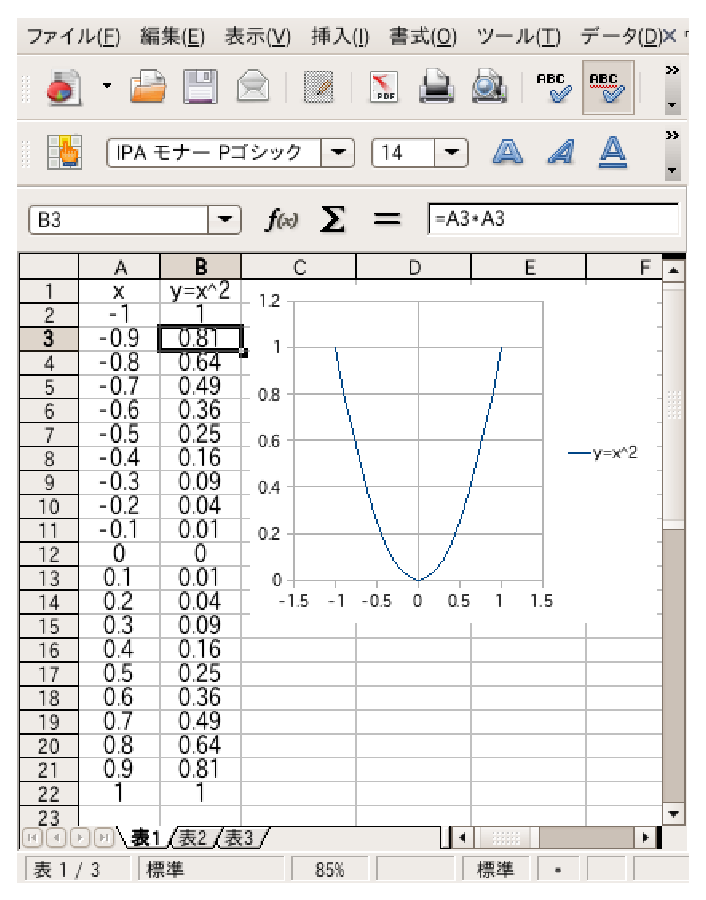
\includegraphics[width=7.3cm]{PC_graph0.eps}
    \caption{$y=x^2$のグラフを描いたところ\label{fig:PC_graph0}}
\end{figure}

\begin{figure}
    \centering
    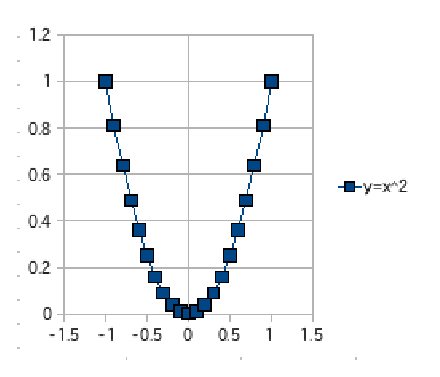
\includegraphics[width=4.5cm]{PC_graph1.eps}
    \caption{グラフ線にマークを入れると見にくい\label{fig:PC_graph1}}
\end{figure}

\begin{faq}{\small\textgt{なぜA1から選ぶのですか? 数値が入っているのは
A2からですよね?} ... それによってセルB1が一緒に選ばれるところがミソです。
そうすることで, B1の内容が, 凡例に表示されるのです。これによって, グラフが
わかりやすくなります。}\end{faq}

\begin{freqmiss}{\small\textgt{関数のグラフを描く時, 横軸の値が不適切な
範囲になる} ... 上の例や下の問で, 「散布図」を選ばずに, 「折れ線」などを選んでしまう
とそうなります。出来上がったグラフをよくチェックしましょう。}\end{freqmiss}

{\small 注: レポートや論文, プレゼン等で使うグラフ(人様に見せるグラフ)をパソコン
で作るときは, 以下に気をつけよう:
\begin{itemize}
\item 複数の関数をひとつのグラフに重ねて描くときは, どの線が
どの関数に対応しているのかを, 必ず凡例などで明記すること。
\item 線の区別をするときは, カラーだけに頼るのではなく, 線の種類
や太さも変えて区別すること(線のどこかをダブルクリックすると, それらを
変更できるウィンドウが出てくる)。これは\textgt{色盲の人への配慮}。
\end{itemize}}

%-----------------------------

{\small 注: 次の問題も含め, 以後, パソコンでグラフを描く問題は, 
レポートではグラフのプリントアウトを掲載せよ。グラフをワープロの
文書にコピー&ペーストすると, レイアウトが楽だし, 複数のグラフを
1枚の紙に印刷するときにも便利。数値データはプリントアウトしなくてもよい。}

\begin{q}\label{q:comp_graph0} パソコンの表計算ソフトを使って, 
次の関数を, $-1 \le x \le 1$の範囲でグラフに描け。重ねて描け。
\begin{edaenumerate}<3>
\item $y=x$
\item $y=x^2$
\item $y=x^3$
\end{edaenumerate}
{\small ヒント: $x$の値は, まとめてひとつの列(A列)にしてよい。B2には「=A2」, C2には「=A2*A2」, D2には「=A2*A2*A2」
と入れて, それぞれ列の下のほう(22行)までコピー・ペースト。B1, C1, D1にそれぞれの関数
の凡例を書き込み(B1には"y=x"とか), A1からD22をマウスで一気に選んでグラフを描けば, 
自動的に3つの線が重なったグラフになる。答えは図\ref{fig:PC_graph2}のようになる。}\end{q}
\begin{figure}
    \centering
    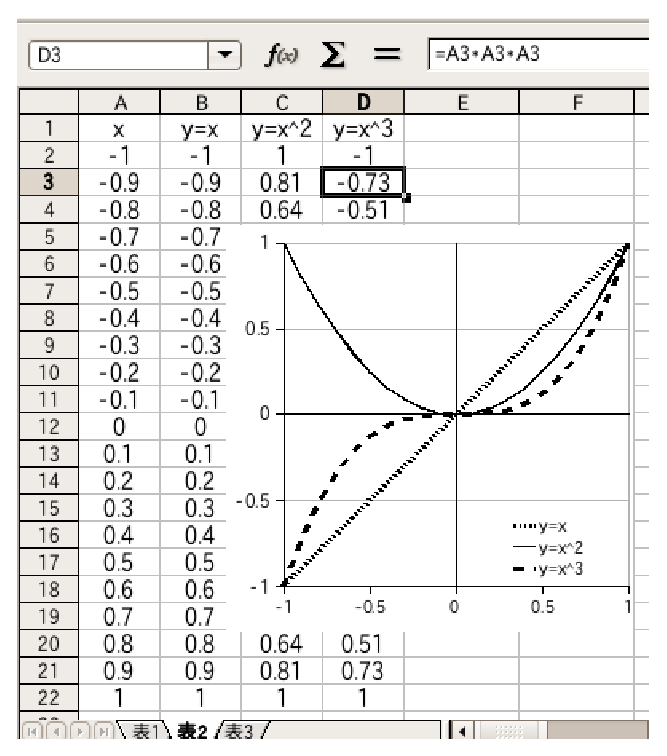
\includegraphics[width=7.0cm]{PC_graph2.eps}
    \caption{$y=x,\, y=x^2,\, y=x^3$のグラフ\label{fig:PC_graph2}}
\end{figure}

\begin{freqmiss}{\small\textgt{複数のグラフを重ねて描くとき, 
どの線が何を表しているかを表示しない} ... そういうレポートは 
減点されるかもしれませんね...}\end{freqmiss}
\hv



\section{関数のグラフと不等式の解}\index{ふとうしき@不等式}

\begin{exmpl}\label{exmpl:ineq001} $x+2<2x-1$という不等式を満たす$x$
はどのような値だろうか? これを式変形すると$3<x$となるから, 
この不等式は$x$が3より大きな値で成立する。\qed\end{exmpl}

\begin{exmpl}\label{exmpl:ineq003} 不等式
\begin{eqnarray}
x^2-x-2<0\label{eq:x2_x_2le0}
\end{eqnarray}
を考える(このように2次式に
関する不等式を2次不等式という)。これを
式変形すると$(x-2)(x+1)<0$である。\eref{eq:th_order_8}
より, $(x-2)$と$(x+1)$は, 片方が負で片方が正のはず。
明らかに$-2<1$だから$x-2<x+1$。小さいほうが負, 大きい方が
正になるはずだから, $x-2<0$かつ$0<x+1$。これを
整理して, $-1<x<2$。これが, この不等式の解。\qed\end{exmpl}

例\ref{exmpl:ineq001}のような単純な不等式は式変形だけで
解けるが, 例\ref{exmpl:ineq003}のような複雑な不等式は, 
ちょっとめんどくさかった。そういうとき, グラフが役立つ。
\eref{eq:x2_x_2le0}の左辺を抜き出して$y=x^2-x-2$という関数
を考えると, そのグラフは図\ref{fig:2Dpoly_graph}の
右端のようになる。\eref{eq:x2_x_2le0}は, この関数を使って$y<0$
と表される。つまり, このグラフが$x$軸よりも下に来るような
ときの$x$の値の範囲を見い出せばよい。明らかにそれは
$-1<x<2$であり, 上の解と一致する。\\

同様に考えれば, 以下の定理が成り立つことがわかるだろう: 
2次方程式$ax^2+bx+c=0$が$x=\alpha$と$x=\beta$という実数解を
持つ時($0<a$, $\alpha<\beta$とする), 不等式
\begin{eqnarray}
ax^2+bx+c<0\label{eq:alg_2ineq_1}
\end{eqnarray}
の解は「$\alpha<x<\beta$」であり, 不等式
\begin{eqnarray}
ax^2+bx+c>0\label{eq:alg_2ineq_2}
\end{eqnarray}
の解は「$x<\alpha$又は$\beta<x$」である。

なぜか? $y=ax^2+bx+c$と
おくと, そのグラフは$x=\alpha$と$x=\beta$で$x$軸と交わり, 
しかも$a>0$なので下に凸の放物線となる。そのグラフが$x$軸
よりも下にある状況や(\eref{eq:alg_2ineq_1}), 上に
ある状況(\eref{eq:alg_2ineq_2})を見い出せばよい。また, 
\eref{eq:alg_2ineq_1}, \eref{eq:alg_2ineq_2}について, 
$<$を$\leq$に置き換えたものについては, その解も
$<$を$\leq$に置き換えたものになることは明らかだろう。

\begin{q}\label{q:alg_ineq1} $x$は実数とする。以下の2次不等式を解け。
\begin{edaenumerate}
\item $x^2+x-6<0$
\item $x^2+5x+6\geq 0$
\item $x^2+3x+1\geq 0$
\end{edaenumerate}
\end{q}

\begin{exmpl} 不等式
\begin{eqnarray}
x^2+x+1>0\label{eq:x2_x_1gt0}
\end{eqnarray}
の解はどうなるだろう?
関数$y=x^2+x+1$のグラフは, 図\ref{fig:2Dpoly_graph}の
左端のようになる。\eref{eq:x2_x_1gt0}は, この関数を使って$y>0$
と表されるから, このグラフが$x$軸よりも上に来るときの
$x$の範囲を言えばよい。といっても, 見るからにこのグラフは
$x$がどんな値でも$x$軸より上にある。従って, 「解は全ての実数」である。\qed\end{exmpl}

\begin{freqmiss}{\small\textgt{↑これを「全ての実数解」という}
 ... なんかおかしくね? 解は何? と聞かれてるんだよ...}\end{freqmiss}

上の例をちょっと変えて, 
\begin{eqnarray}
x^2+x+1<0\label{eq:x2_x_1lt0}
\end{eqnarray}
という不等式の解はどうだろう? そう, 「解なし」だ!

\begin{freqmiss}\label{ex:2dim_ineq_irr}{\small\textgt{
不等\eref{eq:x2_x_1lt0}の解を以下のように間違える:
\begin{eqnarray*}
\frac{-1-\sqrt{3}\,i}{2} < x < \frac{-1+\sqrt{3}\,i}{2}\,\,\,\,\,\, \text{これは間違い!}
\end{eqnarray*}} ... この式には意味がありません。なぜなら, \textgt{虚数には大小関係は存在しない}
からです(例えば, $1+i$とか$5i$はこの「範囲」に入っているかどうか, 言えますか?)。
不等式は普通, 実数の範囲で考えます。}\end{freqmiss}
\mv

\eref{eq:x2_x_1lt0}は, 本来はグラフを使わないで, 以下のように解くべきだ。まず, 
\begin{eqnarray}
\Bigl(x+\frac{1}{2}\Bigr)^2+\frac{3}{4}\label{eq:2dim_ineq_irr5}
\end{eqnarray}
と平方完成する。$(x+\frac{1}{2})^2$は$x$がどんな実数値をとっても0以上だから, 
この式は常に3/4以上。ということは, この式はマイナスになり得ない。従って「解なし」。

このように, 「左辺=0」が実数解を持たないような2次不等式は, 
\eref{eq:2dim_ineq_irr5}のように平方完成して考えねばならない。\hv

\begin{q}\label{q:alg_ineq2}
実数$x$に関する以下の不等式を解け。 
\begin{eqnarray*}
&&(1)\,\,\,\,\,\,\,\,x^2+x+1>0\\
&&(2)\,\,\,\,\,\,\,\,x^2+x+1<0\\
&&(3)\,\,\,\,\,\,\,\,\frac{x+1}{x-1}>0\\
&&(4)\,\,\,\,\,\,\,\,x^2-4x+4<0\\
&&(5)\,\,\,\,\,\,\,\,x^2-4x+4\leq0\\
&&(6)\,\,\,\,\,\,\,\,x^2-4x+4\geq0\\
&&(7)\,\,\,\,\,\,\,\,x^2-4x+4>0
\end{eqnarray*}
{\small ヒント: (3)は分母が0になったら困るから$x\neq1$を前提として, 
両辺に$(x-1)^2$を掛ける。もし, $(x-1)$を両辺にかけてしまうと, 
$x$が1より小さいときに不等号が逆転してしまう(\pref{eq:th_order_3}
の\eref{eq:th_order_3}より)。それを処理するのは面倒。
$(x-1)^2$は0以上だから, 両辺にかけても不等号はかわらない。(4)〜(7)は, 左辺が
$(x-2)^2$であることに注意。}
\end{q}


\section{偶関数・奇関数}
関数$f(x)$が, 恒等的に
\begin{eqnarray}f(-x)=f(x)\end{eqnarray}
を満たすとき, $f(x)$を\underline{偶関数} \index{ぐうかんすう@偶関数}と呼ぶ(定義)。
また, 関数$f(x)$が恒等的に
\begin{eqnarray}f(-x)=-f(x)\label{eq:def_odd_func}\end{eqnarray}
を満たすとき, $f(x)$を\underline{奇関数} \index{きかんすう@奇関数}と呼ぶ(定義)。
偶関数や奇関数は, 他の関数よりも, 何かと扱いが楽である。何か関数を相手に
するときは, まずその関数が偶関数や奇関数か調べよう。もしそうならラッキー!なのだ。\hv

{\small 注: \eref{eq:def_odd_func}を, なぜかわざわざ「$f(x)=-f(-x)$」と変形して
覚える人がいる。間違いではないのだが, この形は, 奇関数の性質を証明する時に
使いづらく, 面倒である。素直に\eref{eq:def_odd_func}の形で覚えよう。}

\begin{q}\label{q:func_evenodd0} 偶関数とは何か? 奇関数とは何か?\end{q}
\mv

既に学んだように, 関数$y=f(x)$のグラフを$y$軸に関して対称移動したら
関数$y=f(-x)$のグラフになる(\ref{sec:func_trans}節の定理5)。ところが
偶関数なら, $f(-x)$はもとの関数$f(x)$に等しい。すなわち, 偶関数のグラフは, 
$y$軸に関して対称移動しても, もとの関数のグラフと一致してしまう。
従って, \textgt{偶関数のグラフは$y$軸に関して対称}である。例えば, 
$y=x^2$は偶関数だが, そのグラフ(図\ref{fig:parab_inverse}左)は
確かに$y$軸に関して対称である。

一方, 関数$y=f(x)$のグラフを原点に関して対称移動したら関数$y=-f(-x)$のグラフに
なる(\ref{sec:func_trans}節の定理6)。ところが, 奇関数なら, 
$-f(-x)$はもとの関数である$f(x)$に等しい。すなわち, 奇関数のグラフは, 
原点に関して対称移動しても, もとの関数のグラフと一致してしまう。
従って, \textgt{奇関数のグラフは原点に関して対称}である。
例えば, $y=ax$ (図\ref{fig:proportion})
や, $y=1/x$や$y=x^3-x$は奇関数だが, それらのグラフ (図\ref{fig:parab_inverse}右, 
図\ref{fig:xxx-x})は確かに原点に関して対称である。

\begin{q}\label{q:func_evenodd1} 以下の各関数$f(x)$について, 偶関数か奇関数か
(もしくはどちらでもないか)を判定し, $y=f(x)$のグラフを描け。
\begin{enumerate}
\item $f(x)=4x^4-5x^2+1$\\ ヒント: $x$軸との交点も考えよ。
\item $f(x)=x+x^2$
\item $f(x)=x-x^3$
\item $f(x)=1/(1+x^2)$\\ ヒント: $x=0$と$x\rightarrow \pm \infty$ではどうなるか? 
\end{enumerate}\end{q}

\begin{faq}{\small\textgt{↑このグラフはパソコンで描くのですか?}
... いえ, 手書きでOK。今後も, 「グラフを描け」は, 「パソコンで」とか「表計算ソフトで」
という指示のある場合はパソコン, それ以外は手書き。}\end{faq}

\begin{freqmiss}{\small\textgt{偶関数の定義を「グラフが$y$軸に関して対称であるような関数」
と言ったり, 奇関数の定義を「グラフが原点に関して対称であるような関数」と言ってしまう}
... それらが定義なら, それらを使って以下の問題を解けますか?}\end{freqmiss}

\begin{q}\label{q:func_evenodd2} 以下を証明せよ:
\begin{enumerate}
\item 偶関数と偶関数の積は偶関数。
\item 奇関数と奇関数の積は偶関数。
\item 偶関数と奇関数の積は奇関数。
\item 偶関数と偶関数の和は偶関数。
\item 奇関数と奇関数の和は奇関数。
\item 偶関数と奇関数の和は, 偶関数でも奇関数でもなくなることがある。(ヒント: 例を挙げればよい。)
\end{enumerate}\end{q}

\begin{q}\label{q:func_evenodd25} 以下の関数について, 偶関数か, 奇関数か, 
いずれでもないか, 判定せよ。
\begin{eqnarray}
f(x)=\Bigl\{(1+x^2+x^4)^3+\frac{1}{x^2+x^4}\Bigr\}^8
\end{eqnarray}\end{q}
↑こんな複雑な関数のグラフなんか, 描ける気がしないだろう。
それでもまだ, 「グラフがなんちゃらに関して対称」とかで偶関数や
奇関数を定義したいなら, なんとかしてグラフを描いてくれ!
\mv

\begin{q}\label{q:func_evenodd28} 関数$f(x)=ax^n$を考える($a$は0以外の任意の実数, $n$は自然数)。$n$が偶数の時は$f(x)$は偶関数であり, $n$が奇数の時は$f(x)$は奇関数であることを証明せよ。\end{q}
\mv

\begin{faq}{\small\textgt{偶関数・奇関数って, 偶数・奇数と関係
ありますか?} ... 言葉が似てるだけに, 前問のように何かしら関係が
あります。また, 問\ref{q:func_evenodd2}で見たことは, 偶数どうしの積が
偶数になるとか, 奇数どうしの積が奇数になるとかに似ています。ただし, 
偶数と奇数の和は奇数だけど, 偶関数と奇関数の和は奇関数とは限りません。
そもそも別の概念だから, どこかが違っているのは当然と言えば当然。}\end{faq}

\begin{faq}{\small\textgt{偶関数の定義を述べよという問題で, 「$f(-x)=f(x)$」と
答えたら不正解になりました。なぜ?}
... 省略しすぎ! せめて「$f(-x)=f(x)$を満たすような関数$f(x)$のこと」
くらいは書かなきゃ, 何のことかわかりません。}\end{faq}
\hv


\section{合成関数}\label{sec:gousei_kansu}
2つの関数$f(x), g(x)$を考える。ある数を$f(x)$に入れると別の数が
返ってくるが, その返ってきた数を次に$g(x)$に入れると, さらに別の
数が返ってくる。このように, 2つの関数$f(x), g(x)$を段階的に続けて
使うことで, 新たな関数ができる。それを「$f(x)$と$g(x)$の
合成関数」\index{ごうせいかんすう@合成関数}といい, $g(f(x))$と書く。
例を見てみよう:

\begin{exmpl} 以下の2つの関数の合成関数を考えよう:
\begin{eqnarray*}
f(x)=x+1,\quad\quad g(x)=x^2
\end{eqnarray*}
例えば$x=1$について, $f(1)=1+1=2$, $g(2)=2^2=4$となる。従って, $g(f(1))=4$である。

合成関数は, 2段めの関数の独立変数$x$に1段めの関数を代入したものである。この場合は, 
\begin{eqnarray}g(f(x))=g(x+1)=(x+1)^2\label{eq:gousei_kansu6}\end{eqnarray}
となる。これに$x=1$を代入すると, 確かに4になる。

\eref{eq:gousei_kansu6}は次のように考えてもよい:
\begin{eqnarray}g(f(x))=\{f(x)\}^2=(x+1)^2\end{eqnarray}
結果は同じである。

合成の順序を変えると, 違った合成関数になることに注意しよう。上の例では, 
\begin{eqnarray}f(g(x))=f(x^2)=x^2+1\label{eq:gousei_kansu7}\end{eqnarray}
である。\eref{eq:gousei_kansu6}と\eref{eq:gousei_kansu7}は明らかに違う関数だ!
(例おわり)\end{exmpl}\mv

$g(f(x))$と書かれるとき, 内側に1段めの関数が, 外側に2段めの関数が
書かれることに注意しよう。左から見ていくと2段めが先に来て1段めが後に来るので, 
順序が混乱する人がいるが, 「何を何に代入するか」と考えれば
自然に納得できるだろう。

\begin{q}\label{q:gouseikansu0} 2つの関数$f(x)=\sqrt{x}$, $g(x)=1+x^2$について, 
$g(f(x))$と$f(g(x))$をそれぞれ求めよ。
\end{q}
\hv


\section{逆関数}\label{sec_gyakukansu}

一般に, 関数$y=f(x)$の$x$と$y$を入れ替えてできる関数$y=g(x)$を, 
関数$f(x)$の\underline{逆関数} \index{ぎゃくかんすう@逆関数}と呼ぶ(定義)。

\begin{exmpl}\label{exmpl:func_inv1} 関数$y=2x$は, $x$と$y$を入れ替えると
$x=2y$となる。これを$y$について解けば$y=x/2$となる。従って, 
$y=2x$の逆関数は$y=x/2$である。(例おわり)\end{exmpl}

\begin{q}\label{q:func_inv0} 以下の関数の逆関数をそれぞれ求めよ。ただし, $a$, $b$は任意の定数とする。
\begin{edaenumerate}
\item $y=2x+1$
\item $y=1/(x-1)$
\item $y=a/x$
\item $y=-x+b$
\end{edaenumerate}
\end{q}\mv

逆関数はどういうイメージのものだろうか? 一般に, 
関数$y=f(x)$を, 数$x$から数$y$への「変換装置」みたいな
ものと考えれば, $x$は「入り口」, $y$は「出口」だ。
従って, $x$と$y$を入れ替えるということは, この装置の
働きを逆行させ, 「出口から入って入り口から出る」ということ。
つまり, $y=f(x)$で変換された数を, 変換前の数に戻す
のが逆関数$y=g(x)$だ。

そう考えると, $g(x)$が$f(x)$の逆関数なら, 逆の立場も言える, つまり
$f(x)$は$g(x)$の逆関数である, ということがわかるだろう。

\begin{exmpl}\label{exmpl:func_inv2} 関数$y=2x$に$x=3$という数を入れると, 
$y=6$という数に変換される。この数を改めて$x$として関数$y=x/2$ (これが$y=2x$の
逆関数であることは例\ref{exmpl:func_inv1}でみたとおり) に入れると, 
$y=6/2=3$となる。確かに最初の$x$の値に戻った。(例おわり)\end{exmpl}\mv

さて, 逆関数にはひとつ面白い性質がある: 
\textgt{$f(x)$と$g(x)$が互いに逆関数であるとき, 恒等的に
\begin{eqnarray}g(f(x))=f(g(x))=x\label{eq:generaleq}\end{eqnarray}
となる}のだ。なぜだろう? 
$f(x)$は, $x$を別の数に移す関数だが, 逆関数$g(x)$はそれを
もとの数$x$に戻す関数だ。だから, $g(f(x))$は, $x$をいったん別の数に移しても
それを元に戻すので, 結局は何もしないに等しい。つまり, $g(f(x))$は$x$をそのまま$x$に
しておく関数である。つまり, 恒等的に$g(f(x))=x$が成り立つ。
同様に, $f(g(x))=x$も恒等的に成り立つ。\qed

\begin{exmpl}\label{exmpl:func_inv3} 例\ref{exmpl:func_inv1}でみた
ように, 関数$y=2x$の逆関数は$y=x/2$である。前者を$f(x)$, 後者を$g(x)$と
してみよう。つまり$f(x)=2x$, $g(x)=x/2$とする。
\begin{eqnarray}
&&f(g(x))=2g(x)=2\times\frac{x}{2}=x\\
&&g(f(x))=\frac{f(x)}{2}=\frac{2x}{2}=x
\end{eqnarray}
確かに\eref{eq:generaleq}が成り立ってる! (例おわり)\end{exmpl}

\begin{q}\label{q:func_inv1} $0\le x$とする。$f(x)=x^2$, $g(x)=\sqrt{x}$について,
 \eref{eq:generaleq}が成り立つことを確かめよ。($x^2$と$\sqrt{x}$は互いに逆関数である。)\end{q}\mv

$f(x)$と$g(x)$が互いに逆関数であるとき, $y=g(x)$は$x=f(y)$と同じことだから, $y=f(x)$のグラフにおいて
$x$軸と$y$軸を取り換えたものが$x=f(y)$, つまり$y=g(x)$のグラフになる
(図\ref{fig:func_revfunc})。

\begin{figure}[h]
    \centering
    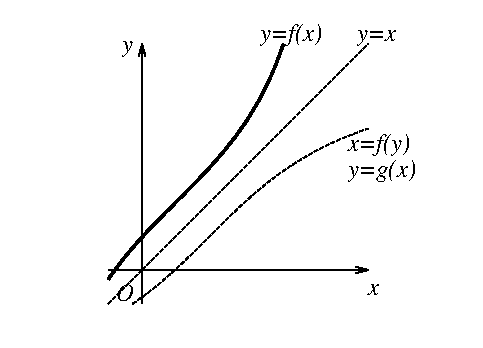
\includegraphics[width=6cm]{func_revfunc.eps}
    \caption{関数$y=f(x)$とその逆関数$y=g(x)$のグラフは$y=x$に関して互いに対称である。\label{fig:func_revfunc}}
\end{figure}

グラフ上で$x$軸と$y$軸を取り換えるときに, 直線$y=x$
だけは不変である。直線$y=x$は$x$軸と$y$軸のちょうど
中間の, 折り返しの位置にあるからだ。あたかも直線$y=x$に
沿って鏡があるように$y=f(x)$のグラフを反転したものが
$x=f(y)$, すなわち$y=g(x)$のグラフになる。従って, 
\textgt{逆関数のグラフはもとの関数のグラフを直線$y=x$に関して対称移動したものだ。}
(だからと言って, これを逆関数の定義としてはいけない。)

\begin{q}\label{q:func_inv2} $y=x^2$と$y=\sqrt{x}$を重ねてグラフに描け.\end{q}

\begin{freqmiss}{\small\textgt{$y=\sqrt{x}$のグラフを, 原点で$y$軸に
突き刺さる角度で描いてしまう} ... $y=x^2$のグラフは放物線なので原点で$x$軸
に接しますよね。$y=\sqrt{x}$はその逆関数なのだから, $y$軸にやさしく接する
はず。突き刺さってはダメ!}\end{freqmiss}

%上で見たように, 逆関数のグラフは$y=x$に関して対称移動したグラフになるので, 
%もともと$y=x$に関して対称なグラフを持つ関数は, 自分自身が自分自身の逆関数になる。\\
\mv

たまに逆関数と逆数を混同する人がいるが, 全く別の概念だ。
たとえば, 例\ref{exmpl:func_inv1}で見たように, $y=2x$の逆関数は$y=x/2$だが, 
$2x$の逆数は$1/(2x)$だ。また, 問\ref{q:func_inv0}で見たように, 
逆関数が自分自身になる関数は多いが, 逆数が自分自身になる数は1と$-1$しかない。\\

\begin{q}\label{q:func_inv3} 次の関数のグラフを, パソコンを使って, \\
$0 \le x \le 1$の範囲で重ねて描け。レポートには, そのグラフのプリントアウトを貼り付けること。
\begin{edaenumerate}<3>
\item $y=x$
\item $y=x^2$
\item $y=x^3$
\item $y=x^4$
\item $y=x^{1/2}$
\item $y=x^{1/3}$
\item $y=x^{1/4}$
\end{edaenumerate}
ヒント: 表計算ソフトでべき乗をするときは\^ \,という記号を使う。
例えばセルA3の3乗は「=A3$\hat{\,\,\,}$3」とする。セルA3の$1/3$乗
は, 「=A3$\hat{\,\,\,}$(1/3)」とする(括弧を忘れないこと!)。
(6), (7)は, 刻みを細かくしよう。
\end{q}

この問でわかるように, $n$を自然数とすると, $y=x^n$のグラフと$y=x^{1/n}$のグラフは, 
直線$y=x$に関して対称である。それらは互いに逆関数だからだ。

また, この形の関数を, 一般に$y=x^\alpha$とおくと, そのグラフは, $\alpha$
によって形が系統的に変わる。この$\alpha$のような数, すなわち
独立変数$x$や従属変数$y$ではなくて関数の性質を決定するような
数のことを, \underline{パラメータ}\index{パラメータ}
% (parameter)
と呼ぶ
\footnote{「パラメータ」と言う言葉には「媒介変数」という別の意味もあるが, それはいずれ説明する。}。
例えば\eref{eq:y_ax_plus_b0}の$a$と$b$もパラメータである。「パラメータが変わるとどうなるか」
という目で関数を理解しよう。そうすると, 「この現象はこういう関数で表現できるのでは?」
という勘が働くようになる。\mv

\begin{faq}{\small\textgt{パソコンでグラフ描くのめんどくさいです。テキストに
載ってるグラフを見るだけでよいのでは?}
... それはダメ。「見るだけ」では心に残らないよ。「見ればわかる」
ことでも, 自分で手を動かしてやってみないと, 心に残らないのです。
人間はそういうもの。このテキストは, パソコンの計算やグラフ描画を通じて
実感・納得するよう設計しています。そのかわり, 他の本にあるような
細かい証明や理屈は載せていません。そうやって学習者の負担を軽くし, 
そのぶん, 生物資源学類で出てくる実例を増やしたり, より高度で
有用な数学を盛り込んでいます。}\end{faq}


\section{陰関数}\index{いんかんすう@陰関数}

今から学ぶのは, ちょっと変わった関数である。いや, 正確には「関数」とは
言えない, 「関数もどき」である。

$y=f(x)$という関数では, $x$の値を代入すれば$y$の値が決まる。しかし, 
ふたつの変数$x, y$を対応づけるのは, このように$y=$の形になっている
関数だけではない。$x^2+xy+y^2-1=0$のように, $x$と$y$が混在する
ような2変数関数が0に等しい, という式でも, いちおう$x$と$y$は対応する。このように, $x$と$y$の
2変数関数$F(x, y)$について, $F(x, y)=0$という方程式で$x$と$y$が対応する場合, この対応関係を
\underline{陰関数} (implicit function)と呼ぶ(定義)。

代表例として, 以下のような陰関数がある。

\begin{q}\label{q:func_circle0} $r$を正の実数の定数とする。陰関数
\begin{eqnarray}
x^2+y^2-r^2=0\label{eq:func_circle0}
\end{eqnarray}
のグラフは(ただし$r>0$とする), 原点を中心とする半径$r$の円になることを示せ。\end{q}
\mv

陰関数を式変形すれば$y=f(x)$の形に整理できることもあるが, 
多くの場合は難しい。ひとつの$x$の値に, 複数の$y$の値が対応する
こともあるからだ。例えば, \eref{eq:func_circle0}は, 
\begin{eqnarray}
y=\pm\sqrt{r^2-x^2}\label{eq:func_circle00}
\end{eqnarray}
と変形できるが, 右辺の$\pm$が嫌らしい。例えば$x=0$に対して
$y=r$と$y=-r$という2つの数が対応してしまう。そもそも関数とは, 
ひとつの$x$に対してひとつの$y$を対応付けるものだ(後に学ぶ「写像」
という概念)。従って, 陰関数は, 厳密な意味では関数ではないのだ。\hv

陰関数にも, グラフの対称性や平行移動, 拡大といった考え方が適用できる。

\begin{exmpl}\label{ex:func_imp0} ある陰関数$F(x,y)=0$の
グラフを$x$軸の正方向に$a$, $y$軸の正方向に$b$だけ平行移動
すると, $F(x-a, y-b)=0$のグラフになる。なぜか?

陰関数$F(x,y)=0$のグラフ上の任意の点Pを考える。その座標を$(x_0, y_0)$とする。
すなわち, $F(x_0, y_0)=0$である。
点Pを$x$軸の正方向に$a$, $y$軸の正方向に$b$だけ平行移動した先の点
を点P$_1$とし, その座標を$(x_1, y_1)$とする。当然, $x_1=x_0+a$
かつ$y_1=y_0+b$である。従って$x_0=x_1-a$
かつ$y_0=y_1-b$である。これを$F(x_0, y_0)=0$に代入すると, 
$F(x_1-a, y_1-b)=0$である。従って, 点P$_1$は陰関数$F(x-a, y-b)=0$
のグラフ上にある。(例おわり)\end{exmpl}

\begin{comment}
一般に, 陰関数$F(x, y)=0$のグラフに関して, 以下の定理が成り立つ
(例\ref{ex:func_imp0}では, 定理1を示した):\\
定理1) $x$軸の正方向に$a$, $y$軸の正方向に$b$だけ平行移動すると, $F(x-a, y-b)=0$のグラフになる。\\
定理2) $x$軸方向に$a$倍, $y$軸方向に$b$倍だけ拡大すると, $F(x/a, y/b)=0$のグラフになる。\\
定理3) $x$軸に関して対称移動すると, $F(x, -y)=0$のグラフになる。\\
定理4) $y$軸に関して対称移動すると, $F(-x, y)=0$のグラフになる。\\
定理5) 原点に関して対称移動すると, $F(-x, -y)=0$のグラフになる。\\
定理6) 恒等的に$F(x, -y)=F(x, y)$なら, $x$軸に関して対称。\\
定理7) 恒等的に$F(-x, y)=F(x, y)$なら, $y$軸に関して対称。\\
定理8) 恒等的に$F(-x, -y)=F(x, y)$なら, 原点に関して対称。\hv

定理2$\sim$定理5の証明は, 形式的には例\ref{ex:func_imp0}で
示した定理1の証明とほぼ同じ。以下にポイントだけを示す:

定理2) $x_1=ax_0$, $y_1=by_0$とする。

定理3) $x_1=x_0$, $y_1=-y_0$とする。

定理4) $x_1=-x_0$, $y_1=y_0$とする。

定理5) $x_1=-x_0$, $y_1=-y_0$とする。

定理6の証明: $F(x, -y)=0$のグラフは, $F(x, y)=0$のグラフを
$x$軸に関して対称移動したもの。ところが, 恒等的に$F(x, -y)=F(x, y)$
なのだから, それは$F(x, y)=0$のグラフに一致するはず。つまり
このグラフは$x$軸に関して対称移動しても元のグラフに一致する。
従って, $x$軸に関して対称である。\qed

定理7, 定理8の証明は, 定理6の証明とほぼ同様。\mv
\end{comment}

\begin{q}\label{q:func_imp1} ($x$, $y$)平面上で, 点$(3, -1)$を中心とする, 半径2の円
を表す陰関数を求めよ。
%\begin{enumerate}
%\item 原点を中心とし, $x$軸方向に径$a$の長軸を持ち, $y$軸方向に径$b$の短軸を
%持つような楕円。ただし$a, b$は正の定数とし, $a>b$とする。
%\end{enumerate}
\end{q}

%\begin{q}\label{q:func_imp2} 以下を示せ。
%\begin{enumerate}
%\item $x^2y^2-1=0$のグラフは, $x$軸に関して対称, 
%$y$軸に関しても対称, 原点に関しても対称。
%\item $x^2+xy+y^2-3=0$のグラフは, 原点に関して対称だが, 
%$x$軸に関して対称ではなく, $y$軸に関しても対称ではない。
%\end{enumerate}
%\end{q}
%問\ref{q:func_imp2}のような陰関数のグラフは, ぱっと思い描くのは難しい。しかし, 
%上で示した定理を使えば, グラフを描く前に, その対称性がわかってしまうのだ。
%数学の論理の素晴らしさはそのようなところにある。
%\hv

\begin{comment}
\begin{exmpl}\label{exmp:func_imp3} $x^2-y^2=1$のグラフを描いてみよう。

まず, このグラフが$x$軸や$y$軸と交わる点を求めよう(なぜなら, $x=0$や$y=0$を
代入するのは簡単だから!)。

$x=0$のときは, $-y^2=1$, つまり$y^2=-1$となり, $y$は実数解を持たない。つまり, 
グラフは$x=0$では点を持たない, すなわち, このグラフは$y$軸を横切ったり$y$軸
に接したりすることはない。

次に, $y=0$のときは, $x^2=1$, つまり$x=\pm1$である。つまりこのグラフは, 
$(1, 0)$, $(-1, 0)$を通る(これが$x$軸との交点)。

次に, グラフの対称性を調べよう。$x^2-y^2-1=0$と変形し, $F(x, y)=x^2-y^2-1$
とすると, この陰関数は, $F(x, y)=0$と書ける。簡単な暗算で, $F(-x, y)=F(x, y)$と
$F(x, -y)=F(x, y)$が成り立つことがわかる。従って, このグラフは$x$軸と$y$軸の
それぞれに関して対称である(上の定理6と定理7)。

次に, $x$や$y$がどんどん大きくなるとこのグラフはどうなるか, 調べよう。
$x$や$y$が1000や10000のように大きな数になると, $F(x, y)=x^2-y^2-1=0$で示される
$x$と$y$の関係の中では, 定数項である「$-1$」は, 相対的に無視できる
(100万円や1億円を持っている人は, 1円にはこだわらない!)。
従って,  この陰関数は, $x^2-y^2\fallingdotseq0$となる。因数分解すると, 
$(x-y)(x+y)\fallingdotseq0$すなわち, $x-y\fallingdotseq0$または$x+y\fallingdotseq0$
となる。つまり, 直線$y=x$または直線$y=-x$に次第に近づく。これらが漸近線である。

これだけの手がかりで, ほとんどグラフは描けるが, 心配な人のために, もうひと押ししよう。
この陰関数は, $y^2=x^2-1$, すなわち$y=\pm\sqrt{x^2-1}$と変形できる。
$0<x, 0<y$の範囲(つまりグラフの第一象限\footnote{$0<x,\, 0<y$の領域。
$x$軸と$y$軸で区切られる平面の右上部分のこと。})に限定すると, $y=\sqrt{x^2-1}$
であり, この関数は$x$に関して単調に増加する。従って, $x$が大きくなるに従って, 
点$(1, 0)$から, 漸近線$y=x$に向けて単調に近づく線を描くはずだ。それを対称性
によって$y$軸の左側や$x$軸の下側にコピーする。結果として, 
図\ref{xx_minus_yy_eq_1}のようなグラフになる\footnote{実は, 図\ref{xx_minus_yy_eq_1}は, 
\pref{fig:parab_inverse}の図\ref{fig:parab_inverse}右で見たような双曲線を回転させたものになっている。正確に言うと, 
$y=1/(2x)$で表される双曲線を, 90度, 右回りに回転させたのが図\ref{xx_minus_yy_eq_1}である。}。
なお, なぜか図\ref{fig:hyperbola_NG}のように漸近線から離れて行くグラフを描いてしまう人がいるので注意!
\begin{figure}
    \centering
      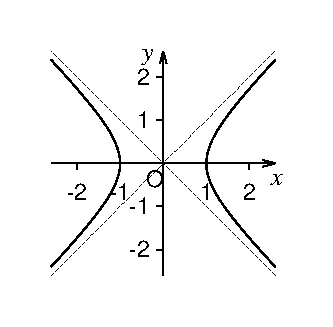
\includegraphics[width=5cm]{xx_minus_yy_eq_1.eps}
      \caption{$x^2-y^2=1$のグラフ。点線は漸近線($y=\pm x$)。\label{xx_minus_yy_eq_1}} 
\end{figure}
(例おわり)\end{exmpl}
\hv

\begin{q}\label{q:func_imp4} 以下の関数について, それぞれグラフを描け。漸近線がある場合は
漸近線を点線で描き込み, その方程式も述べよ。:
\begin{edaenumerate}
\item $x^2-y^2=-1$
\item $4x^2-y^2=1$
\item $x^2-y^2=9$
\item $x^2+y^2/4=1$
\end{edaenumerate}\end{q}

\begin{figure}
    \centering
      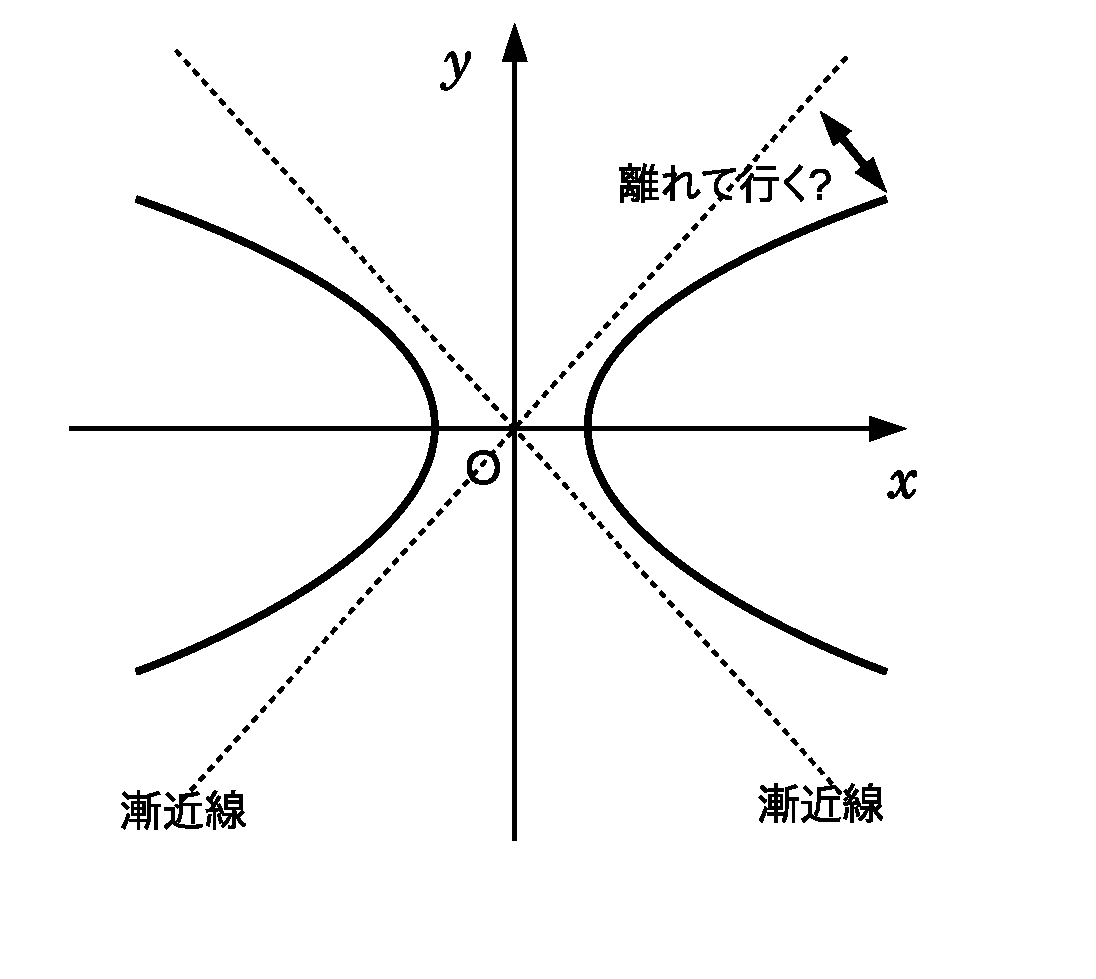
\includegraphics[width=5cm]{hyperbola_NG.eps}
      \caption{よくある\textgt{\large{ダメな}}グラフ。漸近線は
グラフが近づいて行く線なので, 離れて行くのは間違い!\label{fig:hyperbola_NG}} 
\end{figure}
\hv
\end{comment}

\section{関数のグラフを描く手順}
ここで, 関数のグラフを手で描く手順をまとめておこう:
\begin{itemize}
\item $x$の全範囲で関数はつながっているかチェック。$1/x$のように割り算が入った関数は, 「0での割り算」の
ところで関数が途切れる。陰関数は, $x$のとりうる範囲がかなり限定されることもある
(例えば$x^2+y^2=1$は$-1\le x \le 1$でしか定義されない)。
\item $x=0$での$y$の値($y$軸との共有点)を調べる。無いとき(虚数解になるとき)はグラフは$y$軸を通らない。
\item $y=0$での$x$の値($x$軸との共有点)を調べる。無いとき(虚数解になるとき)はグラフは$x$軸を通らない。
\item 関数の対称性を調べる($x$を$-x$にしてみたり$y$を$-y$にしてみたり)。
\item よく知っている関数の平行移動や拡大, 縮小, 対称移動, 和などにならないか調べる。
\item $x$や$y$が$\infty$や$-\infty$に行くときの様子を調べる。
%\item 漸近線があるかどうか, 調べる。
\item それでもよくわからないときは, $x$に適当な数(なるべく計算しやすい値)
をいくつか代入して$y$の値を求め, グラフにプロットしてみる。
\end{itemize}

\begin{faq}{\small\textgt{高校で数IIIを習ったときは, 関数を微分して増減表を
作って, それをもとに関数のグラフを描きました。それじゃダメですか?}
... もちろんいいですよ。でも, ここで学んだ, 「微分を使わないやり方」も有用です。
複雑な関数, 特に陰関数は, 微分したりそれが0になる$x$を求めたりが大変だったり
するからね。それに, 漸近線は増減表からは出ないよね。ここでやったように, 関数の
おおまかな性質を検討するだけでも, いろんな関数のグラフを, 漸近線を
含めてうまく描けます。そういう大局的な見方は, いろんな関数をイメージする
ための強力な武器です。実際, 複雑な関数のグラフはパソコンで描け
ばいいのですが, それを正しく行い, 結果を吟味するには, 
ここで学んだ考え方が有用なのです。}\end{faq}
\hv


\section*{演習問題}

\begin{exq}\label{q:Michaelis_Menten} 次式は, 酵素が介在する
化学反応の速度を説明する, ミカエリス・メンテンの式というものである: 
\begin{eqnarray}
v=\frac{V_{\text{max}}[S]}{K_{\text{m}}+[S]}\label{eq:Michaelis_Menten0}
\end{eqnarray}
$V_{\text{max}}$と$K_{\text{m}}$は正の定数。
$v$は化学反応の速度(単位時間あたり, 単位体積あたりに生成される
化学物質の量), $[S]$は基質(化学反応の材料となる物質)の濃度である。
この式は, $v$を$[S]$の関数として表している。
\begin{enumerate}
\item $[S]=0$のとき$v=0$であることを示せ。
\item $[S]\rightarrow\infty$の極限で, $v$は$V_{\text{max}}$に限りなく近づいていくことを示せ。
\item $[S]=K_{\text{m}}$のとき, $v=V_{\text{max}}/2$となることを示せ。
\item 以上を参考にして, \eref{eq:Michaelis_Menten0}のグラフを描け。
横軸を$[S]$, 縦軸を$v$とせよ。基質の濃度は0以上なので, $0\leq[S]$としてよい。
\item $y=1/v$, $x=1/[S]$として, \eref{eq:Michaelis_Menten0}を$y$と$x$の関係式(一次式)に変形せよ。
それをグラフに描いた時, 切片と傾きにはどのような意味があるか?
\end{enumerate}\end{exq}\mv

{\small 参考(酵素化学が専門の橋本義輝先生のコメント): 学生はミカエリスメンテン式を, $V_{\text{max}}$と$K_{\text{m}}$
が決まってるので任意の$[S]$の時の$v$がわかる式と理解しているようです。しかし, 酵素学では, $V_{\text{max}}$と$K_{\text{m}}$にそれぞれ意味があるので、実験的に求めた複数の$[S]$と$v$の関係からミカエリスメンテン式を使って$V_{\text{max}}$と$K_{\text{m}}$を求めることになります(表裏一体で、どちらから眺めるかの違いですが...)。}

%\begin{exq}\label{q:func_1_1_x2} 以下の関数のグラフを描け。漸近線がある場合は
%漸近線を点線で描き込み, その方程式も述べよ。
%\begin{eqnarray}
%y=\frac{1}{1-x^2}
%\end{eqnarray}
%ヒント: 分母が0になるような$x$では, グラフは発散して途切れる。
%よくわからない, という人は, $x$に$0, 0.1, 0.5, 0.9, 1.1, 2, 3$などの
%値を代入してみよ。
%\end{exq}

\begin{exq}\label{q:func_evenodd_gousei} $K_1(x), K_2(x)$を奇関数, 
$G_1(x), G_2(x)$を偶関数とする。以下の関数を, 奇関数か, 偶関数か, 
どちらとも言えないか, 示せ(根拠も述べよ)。
\begin{edaenumerate}
\item $K_1(K_2(x))$
\item $G_1(G_2(x))$
\item $K_1(G_1(x))$
\item $G_1(K_1(x))$
\item $K_1(x)$の逆関数
\item $G_1(x)$の逆関数
\end{edaenumerate} 
\end{exq}\mv

%\begin{exq}\label{q:func_even_and_odd} 奇関数であり, なおかつ偶関数
%でもあるような関数はあるか? あるなら, どのような関数か? 
%根拠も述べよ。ヒント: 陰関数は関数ではないので除外して考える。\end{exq}

\begin{exq}\label{q:func_imp_th2} 陰関数$F(x, y)=0$のグラフに関して, 
\begin{enumerate}
\item $x$軸に関して対称移動すると, $F(x, -y)=0$のグラフになることを示せ。
\item 恒等的に$F(x, -y)=F(x, y)$なら, $x$軸に関して対称であることを示せ。
\item $x$軸方向に$a$倍, $y$軸方向に$b$倍だけ拡大すると, $F(x/a, y/b)=0$のグラフになることを示せ。
\item 以上を参考にして, 以下の2つの陰関数のグラフをそれぞれ描け:\\
(1)  $x^2-y^2=1$   (2)  $(x^2/4)+(y^2/9)=1$
\end{enumerate}
\end{exq}\mv

%\begin{exq}\label{q:func_inverse_invariant} (発展)
%\begin{enumerate}
%\item 一般に, 関数$f(x)$のグラフが直線$y=x$に関して対称であれば, その
%関数の逆関数は自分自身であることを証明せよ。
%\item 問\ref{q:func_inv0}の関数以外で, 逆関数が自分自身になるような
%関数の例を3つ挙げよ(定数や係数の値だけが異なるものは認めない)。
%% F(x, y)=F(y, x)となる陰関数でF(x, y)=0としたものをyについて解けばよい。
%\end{enumerate}
%\end{exq}

%\begin{exq}\label{q:function_English} 以下の言葉を英訳せよ:
%\begin{edaenumerate}
%\item 関数
%\item 極限
%\item 独立変数
%\item パラメータ
%\end{edaenumerate}
%\end{exq}\mv
\hv



\section*{問題の解答}

%\noindent{\textbf{答}}\ref{q:func_trans0}  略(実際に各点を$xy$平面にプロットしてみよ)。\mv

\noindent{\textbf{答}}\ref{q:func_trans1}  $y=f(x)$の
グラフ上の任意の点Pを考える。その座標を$(x_0, y_0)$とする。
$y_0=f(x_0)$が成り立つ。

定理2の証明: 点Pを$x$軸方向に$a$倍して移動した先の点,
すなわち$(ax_0, y_0)$を, あらためて点P$_2$とし, 
その座標を$(x_2, y_2)$と置く。すなわち, 
$x_2=ax_0,\, y_2=y_0$である。すなわち, $x_0=x_2/a, y_0=y_2$
である。これを$y_0=f(x_0)$に代入すると, $y_2=f(x_2/a)$となる。
従って, 点P$_2$は$y=f(x/a)$のグラフの上にある。\qed

%定理3$\sim$定理6の証明は, 定理2の証明と形式的には
%ほぼ同じである。以下にポイントだけを示す(君はちゃんとやること!)。

%定理3では, 移動先の点$(x_0, ay_0)$を点P$_3$とし, 
%その座標を$(x_3, y_3)$とする。

定理4の証明: 点Pを$x$軸に関して対称移動した先の点, 
すなわち$(x_0, -y_0)$を, あらためて点P$_4$とし, 
その座標を$(x_4, y_4)$と置く。すなわち, 
$x_4=x_0,\, y_4=-y_0$である。すなわち, $x_0=x_4, y_0=-y_4$
である。これを$y_0=f(x_0)$に代入すると, $-y_4=f(x_4)$, 
すなわち$y_4=-f(x_4)$となる。従って, 点P$_4$は
$y=-f(x)$のグラフの上にある。\qed
\mv

\noindent{\textbf{答}}\ref{q:func_trans2}  
\begin{enumerate}
\item $y=(x-1)^{2}+2$
\vspace{0.1cm}
\item $y=3(x/2)^2=3x^2/4$
\vspace{0.1cm}
\item $y=x^2$を(図\ref{fig:x2_trans}左上), まず$x$軸方向に2倍することで, 
\begin{eqnarray}y=\Bigr(\frac{x}{2}\Bigl)^2\end{eqnarray}
になる(図\ref{fig:x2_trans}中上)。さらに$x$軸方向に1移動することで, 
\begin{eqnarray}y=\Bigr(\frac{x-1}{2}\Bigl)^2\end{eqnarray}
になる(図\ref{fig:x2_trans}右上)。
\item $y=x^2$を(図\ref{fig:x2_trans}左下), まず$x$軸方向に1移動することで, 
\begin{eqnarray}y=(x-1)^2\end{eqnarray}
になる(図\ref{fig:x2_trans}中下)。さらに$x$軸方向に2倍することで, 
\begin{eqnarray}y=\Bigr(\frac{x}{2}-1\Bigl)^2\end{eqnarray}
になる(図\ref{fig:x2_trans}右下)。
\end{enumerate}
\begin{figure}[h]
    \centering
      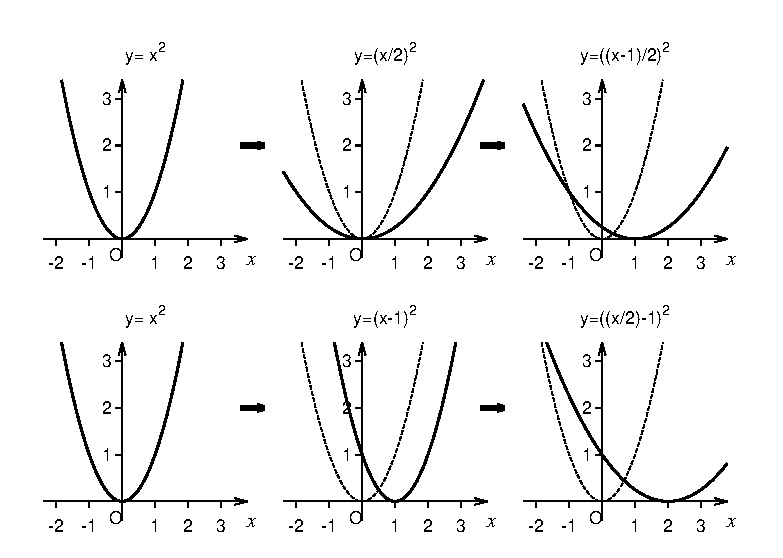
\includegraphics[width=7.0cm]{x2_trans.eps}
      \caption{$y=x^2$の2段階の変形。順序が違えば結果も違う。点線は$y=x^2$。\label{fig:x2_trans}}
\end{figure}


\noindent{\textbf{答}}\ref{q:func_trans3}  図\ref{2x_plus_1_etc}参照。
\begin{enumerate}
\item $y=2x$のグラフを上に($y$軸方向に)1移動。
\item $y=(x+1)^2+2$だから, $y=x^2$のグラフを左($x$軸の負の方向)に1, 上に2移動。
\item $y=1/x$のグラフを上($y$軸の正の方向)に2移動。
\item $y=2-2/(x+1)$だから, $y=1/x$のグラフを縦に2倍し, 上下反転し, 左($x$軸の負の方向)に1, 上に2移動。
$x=0$のときに$y=0$となるので, 原点を通る。
\end{enumerate}

\begin{figure}[h]
    \centering
      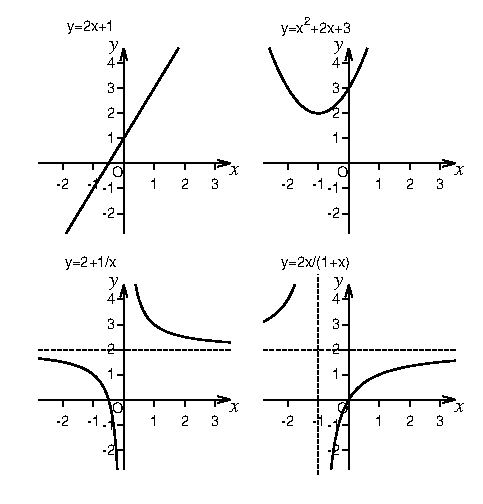
\includegraphics[width=6cm]{2x_plus_1_etc.eps}
      \caption{問\ref{q:func_trans3}のこたえ。点線は漸近線。\label{2x_plus_1_etc}}
\end{figure}
\mv

\noindent{\textbf{答}}\ref{q:func_line0} 
\begin{enumerate}
\item $y=3x-2$
\item \eref{eq:lineeq}より, $y=2(x+1)+1$, \\すなわち$y=2x+3$。
\item \eref{eq:lineeq2p}より, 
\begin{eqnarray}y=\frac{-3-1}{4-2}(x-2)+1\end{eqnarray}
すなわち$y=-2x+5$。
\end{enumerate}
\mv

\noindent{\textbf{答}}\ref{q:Fahrenheit} 
\begin{enumerate}
\item $(32, 0)$と$(212, 100)$を通る一次関数(直線の式)を求めればよい。
\begin{eqnarray*}
&&y-0=\frac{100-0}{212-32}(x-32)\quad\text{すなわち, }\\
&&y=\frac{5}{9}(x-32)=\frac{5}{9}\,x-\frac{160}{9}
\end{eqnarray*}
\item
\begin{eqnarray*}
x=\frac{9}{5}\,y+32
\end{eqnarray*}
\item 以下略
\end{enumerate}
\mv
%\noindent{\textbf{答}}\ref{q:x_plus_1_over_x} 略。\mv

%\noindent{\textbf{答}}\ref{q:read_a_graph} 略。\mv

%\noindent{\textbf{答}}\ref{q:read_a_graph_line} 略。\mv

% パソコンの表計算ソフトを使って, 次の関数を, $-1 \le x \le 1$の範囲でグラフにかけ
%\noindent{\textbf{答}}\ref{q:comp_graph0}  略。

% 不等式
%\noindent{\textbf{答}}\ref{q:alg_ineq0} まず$a<b\text{かつ}(x-a)(x-b)<0$とする。\eref{eq:th_order_8}より, $(x-a)$と$(x-b)$の片方は負, もう片方は正。
%ところが, $a<b$より, $-b<-a$。両辺に$x$を足すと, $x-b<x-a$。従って, $x-b$が負で, $x-a$が正である。つまり$x-b<0$かつ$0<x-a$。前者から$x<b$, 後者から$a<x$。この両方が成り立つはずだから, $a<x<b$ (\eref{eq:alg_2ineq_1}の証明おわり)。\\
%次に, $a<b\text{かつ}(x-a)(x-b)>0$とする。\eref{eq:th_order_7}より, $(x-a)$と$(x-b)$は同符号。ともに正のときは, $0<x-a$かつ$0<x-b$。すなわち$a<x$かつ$b<x$。ところが, $a<b$より, $b<x$であれば$a<x$は自動的に成り立つ。従って, $b<x$を満たすだけでよい。一方, ともに負のときは, $x-a<0$かつ$x-b<0$。すなわち$x<a$かつ$x<b$。ところが, $a<b$より, $x<a$であれば自動的に$x<b$が成り立つ。従って, $x<a$を満たすだけでよい。以上から, $x<a$または$b<x$
%(\eref{eq:alg_2ineq_2}の証明おわり)。\qed

\noindent{\textbf{答}}\ref{q:alg_ineq1} 
\begin{enumerate}
\item 左辺=0の解は$x=-3, 2$。$\therefore\,-3<x<2$
\item 左辺=0の解は$x=-3, -2$。$\therefore\,x \leq -3,\, -2 \leq x$
\item 左辺=0の解は$x=\frac{-3\pm\sqrt{5}}{2}$。よって, 
\begin{eqnarray*}
x \leq \frac{-3-\sqrt{5}}{2},\,\,\, \frac{-3+\sqrt{5}}{2} \leq x
\end{eqnarray*}
\end{enumerate}

\noindent{\textbf{答}}\ref{q:alg_ineq2} 
\begin{enumerate}
\item 左辺=$(x+1/2)^2+3/4$。これは$x$がどんな実数値でも正の値をとる。従って, この不等式は, すべての実数値$x$について成り立つ。
\item 前問と同様に考えれば, この不等式はどんな実数値にも成り立たない(解を持たない)。
\item (略解) $x<-1,\, 1<x$
\item (略解) 解なし。
\item (略解) $x=2$
\item (略解) 全ての実数。
\item (略解) 2以外の全ての実数。
\end{enumerate}
\mv

\noindent{\textbf{答}}\ref{q:func_evenodd0} 略。「グラフがなんとかに関して対称」とか
書いてしまった人は, もっと真剣に本文を読もう!
\mv

\noindent{\textbf{答}}\ref{q:func_evenodd1}  グラフは図\ref{xxxx_minus_etc}参照。
\begin{enumerate}
\item 偶関数。$y=(x+1)(2x+1)(2x-1)(x-1)$なので, $x$軸との交点は$x=-1, -1/2, 1/2, 1$。
$x\rightarrow \pm \infty$で, $y\rightarrow \infty$。
\item どちらでもない。$y=(1+x)x$なので, $x$軸との交点は$x=-1, 0$。$y=(x+1/2)^2-1/4$なので, 
$y=x^2$のグラフを左に$1/2$, 下に$1/4$移動。
\item 奇関数。$y=-(x+1)x(x-1)$なので, $x$軸との交点は$x=-1, 0, 1$。
$x\rightarrow \infty$で, $y\rightarrow -\infty$。
$x\rightarrow -\infty$で, $y\rightarrow \infty$。
(本文の例\ref{exmpl:func_xxx_x}の, $y=x^3-x$のグラフ, つまり図\ref{fig:xxx-x}を, 上下反転したものとも言える。)
\item 偶関数。$x\rightarrow \pm \infty$で, $y\rightarrow 0$。つまり$x$軸に漸近する。
$x=0$のとき$y=1$。ピークを尖らせたらダメ!
\end{enumerate}
\mv

\begin{figure}[h]
    \centering
      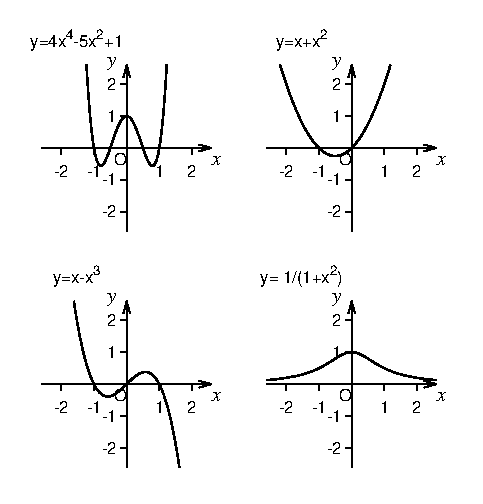
\includegraphics[width=8.5cm]{xxxx_minus_etc.eps}
      \caption{問\ref{q:func_evenodd1}のこたえ。\label{xxxx_minus_etc}}
\end{figure}

\noindent{\textbf{答}}\ref{q:func_evenodd2}  $f_1(x),\, f_2(x)$を任意の偶関数, 
$g_1(x),\, g_2(x)$を任意の奇関数とする。定義より, 
\begin{eqnarray*}
&&f_1(-x)=f_1(x),\quad f_2(-x)=f_2(x)\\
&&g_1(-x)=-g_1(x),\quad g_2(-x)=-g_2(x)
\end{eqnarray*}
である。さて, 
\begin{enumerate}
\item $F(x)=f_1(x)f_2(x)$とすると, 
\begin{eqnarray*}
F(-x)=f_1(-x)f_2(-x)=f_1(x)f_2(x)=F(x)
\end{eqnarray*}
従って, $F(x)$は偶関数。\qed
\vspace{0.1cm}
\item $F(x)=g_1(x)g_2(x)$とすると, 
\begin{eqnarray*}
F(-x)&=&g_1(-x)g_2(-x)=\{-g_1(x)\}\{-g_2(x)\}\\
     &=&g_1(x)g_2(x)=F(x)
\end{eqnarray*}
従って, $F(x)$は偶関数。\qed
\vspace{0.1cm}
\item $F(x)=f_1(x)g_1(x)$とすると, 
\begin{eqnarray*}
F(-x)&=&f_1(-x)g_1(-x)=f_1(x)\{-g_1(x)\}\\
     &=&-f_1(x)g_1(x)=-F(x)
\end{eqnarray*}
従って, $F(x)$は奇関数。\qed
\vspace{0.1cm}
\item $F(x)=f_1(x)+f_2(x)$とすると, 
\begin{eqnarray*}
F(-x)=f_1(-x)+f_2(-x)=f_1(x)+f_2(x)=F(x)
\end{eqnarray*}
従って, $F(x)$は偶関数。\qed
\vspace{0.1cm}
\item $F(x)=g_1(x)+g_2(x)$とすると, 
\begin{eqnarray*}
F(-x)&=&g_1(-x)+g_2(-x)=-g_1(x)-g_2(x)\\
     &=&-\{g_1(x)+g_2(x)\}=-F(x)
\end{eqnarray*}
従って, $F(x)$は奇関数。\qed
\vspace{0.1cm}
\item 例えば偶関数$y=1$と奇関数$y=x$の和: $y=1+x$は, 偶関数でも奇関数でもない。\qed
\end{enumerate}
\mv

\noindent{\textbf{答}}\ref{q:func_evenodd25} 略解: $f(-x)=f(x)$となることは
暗算でも確認できる。答は偶関数。注: $f(-x)=f(x)$を満たせば偶関数なのだから(それが定義), 
それを確認すれば十分である。グラフなど描く必要はない。\mv

\noindent{\textbf{答}}\ref{q:gouseikansu0}
$g(f(x))=1+x$ (ただし$x\ge0$), $f(g(x))=\sqrt{1+x^2}$\mv

\noindent{\textbf{答}}\ref{q:func_inv0} 
\begin{enumerate}
\item $x$と$y$を入れ替えると$x=2y+1$。変形すると, $y=(x-1)/2$。
\item $x$と$y$を入れ替えると$x=1/(y-1)$。変形すると, $y=1+1/x$。
\item $x$と$y$を入れ替えると$x=a/y$。変形すると, $y=a/x$。
\item $x$と$y$を入れ替えると$x=-y+b$。変形すると, $y=-x+b$。
\end{enumerate}
注: (3), (4)では逆関数が自分自身になっていることに注意せよ。\mv

\noindent{\textbf{答}}\ref{q:func_inv1} $g(f(x))=\sqrt{f(x)}=\sqrt{x^2}=|x|$。$x$は0以上だから, これは$x$に恒等的に等しい。また, 
$f(g(x))=(g(x))^2=(\sqrt{x})^2=x$。
\mv

\noindent{\textbf{答}}\ref{q:func_inv2} 図\ref{xx_and_sqrt_x}参照。
\mv

\noindent{\textbf{答}}\ref{q:func_inv3} 図\ref{x_or_xx_etc}参照。
\mv

\begin{figure}[h]
    \centering
      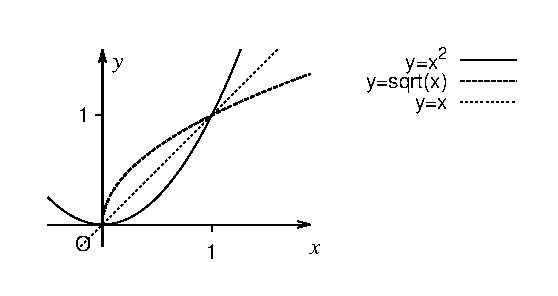
\includegraphics[width=7cm]{xx_and_sqrt_x.eps}
      \caption{問\ref{q:func_inv2}の答。図中, "sqrt(x)"とあるのは$\sqrt{x}$のこと。
直線$y=x$に関して対称であることに注意。どの線も点$(1, 1)$を通る。\label{xx_and_sqrt_x}}
\end{figure}

\begin{figure}[h]
    \centering
      
\includegraphics[width=7cm]{x_or_xx_etc.eps}
      \caption{問\ref{q:func_inv3}の答。$y=x$の上側にあるのが, $x^{1/2},\, x^{1/3},\, x^{1/4}$。
どの線も点$(1, 1)$を通る。\label{x_or_xx_etc}}
\end{figure}

\noindent{\textbf{答}}\ref{q:func_circle0} 三平方の定理より$x^{2} + y^{2}$は, 原点から点$(x,\,y)$までの距離の二乗。与式より, 
これが$r^2$に常に等しいので, 原点から各点までの距離は常に$r$である。原点から一定距離$r$
にある点の集合は, 原点を中心とする半径$r$の円である。\qed
\mv

\noindent{\textbf{答}}\ref{q:func_imp1} 
原点中心, 半径$2$の円を表す陰関数は, \eref{eq:func_circle0}で$r=2$として, 
$x^2+y^2-4=0$。これを$x$方向に3, $y$方向に$-1$だけ移動すると(例\ref{ex:func_imp0}より), \\
$(x-3)^2+(y+1)^2-4=0$。\mv
%\item 原点中心, 半径$1$の円を表す陰関数は, $x^2+y^2-1=0$。これを$x$軸方向に$a$倍, 
%$y$軸方向に$b$倍だけ伸ばすと(定理2より), 
%\begin{eqnarray}\frac{x^2}{a^2}+\frac{y^2}{b^2}-1=0\end{eqnarray}
%\end{enumerate}

\begin{comment}
\noindent{\textbf{答}}\ref{q:func_imp2}
\begin{enumerate}
\item $F(x, y)=x^2y^2-1$とする。任意の$x, y$について, 
$F(-x, y)=F(x, -y)=F(-x, -y)=F(x, y)$が恒等的に成り立つので, 
定理5, 6, 7より, $F(x, y)=0$のグラフは$x$軸と$y$軸と原点に
関して対称。\qed
\item $F(x, y)=x^2+xy+y^2-3$とする。任意の$x, y$について, 
$F(-x, -y)=F(x, y)$が恒等的に成り立つので原点対称。しかし, 
点$(1, 1)$は$F(x, y)=0$を満たすが, その点を$x$軸と$y$軸に
関してそれぞれ対称に移動した点$(-1, 1)$と$(1, -1)$は, $F(x, y)=0$
を満たさないので, このグラフ上には存在しない(反例)。従って, この
グラフは$x$軸に関しても$y$軸に関しても対称ではない。\qed
\end{enumerate}
\hv

\noindent{\textbf{答}}\ref{q:func_imp4} 図\ref{4xx_minus_yy_eq_1_etc}参照。
(1)では, $y=\pm\sqrt{x^2+1}$となるが, $x$が十分に大きいと根号の中の1は
$x^2$よりずっと小さいので無視でき, $y\fallingdotseq\pm\sqrt{x^2}=\pm x$と
なる。従って, $y=x$と$y=-x$が漸近線。(2)では, $y=\pm\sqrt{4x^2-1}$となるが, 
$x$が十分大きい時は, $y\fallingdotseq\pm\sqrt{4x^2}=\pm2x$となる。従って, 
$y=2x$と$y=-2x$が漸近線。(3)では, $y=\pm\sqrt{x^2-9}$となるが, 
$x$が十分大きい時は, $y\fallingdotseq\pm\sqrt{x^2}=\pm x$となる。従って, 
$y=x$と$y=-x$が漸近線。(4)では漸近線は存在しない(なぜなら, $x$が大きな数に
なると$y$は虚数になるし, $y$が大きな数になると$x$は虚数になる。虚数の点は
グラフには現れない)。

\begin{figure}
    \centering
    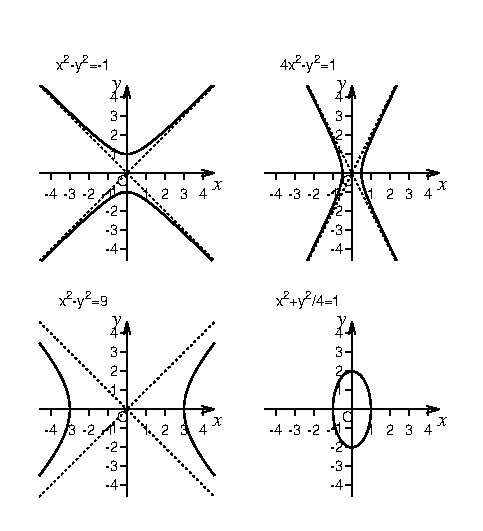
\includegraphics[width=7cm]{4xx_minus_yy_eq_1_etc.eps}
    \caption{問\ref{q:func_imp4}のこたえ。それぞれ, 点線は漸近線。}\label{4xx_minus_yy_eq_1_etc}
\end{figure}
\vv
\end{comment}




\include{04_function_ans}
\chapter{微分}

{\small 過去の受講生の言葉: 「わかろうとしすぎないと, いつのまにかわかり出す。」}

\section{微分の定義}\label{sect_def_differential}

これからいよいよ「微分」というのを学ぶ。まず微分の発想を説明しよう。
何か関数$y=f(x)$を考える。そのグラフの形はどんなでもいいけど, 
\fref{fig:diff_explain}のようになめらかに連続的につながっている
としよう。今, 実数$x_0$を固定して考え, 点$(x_0, f(x_0))$を
点Pと名付ける。また, $x_0$に近い(けど$x_0$ではない)実数$x$を
考え, $(x, f(x))$を点Qと名付ける。

\begin{figure}[h]
    \centering
    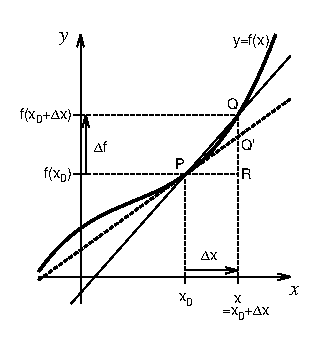
\includegraphics[width=7cm]{diff_explain.eps}
    \caption{関数$y=f(x)$のグラフ(太い実線)と, 点Pにおける接線のグラフ
(太い点線), そして$y=f(x)$上の2点P, Qを通る直線(細い実線)のグラフ。なお, 
原点$O$はどこにあるか定かでない(というか問題にならない)のでこのグラフには
書き込んでいない。}
\label{fig:diff_explain}\end{figure}

ここで, 点Pにおける接線(点Pでこの関数に接する直線; 
\fref{fig:diff_explain}の太い点線)を考えよう。その傾きを$a$とすると, 
この接線は点P$(x_0, f(x_0))$を通る, 傾き$a$の直線なので, 
その関数は$y=f(x_0)+a(x-x_0)$となる。

さて, もし$x_0$と$x$との間隔が十分に狭ければ, そのあたりでは, 
この関数のグラフ(\fref{fig:diff_explain}の太い実線)は, 
点Pにおける接線(\fref{fig:diff_explain}の太い点線)でざっくりと
近似できるだろう。すなわち, 次式が成り立つだろう:
\begin{eqnarray}
f(x) \fallingdotseq f(x_0)+a(x-x_0)\label{eq:define_dif0}
\end{eqnarray}
ここで"$\fallingdotseq$"は, 「ほぼ等しい」「近似的に等しい」という
意味の記号だ。\eref{eq:define_dif0}の左辺は点Qの$y$座標で, 
右辺は点Q'の$y$座標だ。点Qと点Q'は微妙にズレているので, 
=でなく$\fallingdotseq$と書くのだ。

先回りしてざっくり言えば, 微分というのは, この定数$a$
(接線の傾き)のことだ。でも, そこには深くて微妙な話があるので, 
しばらく辛抱して続きを読んで欲しい。

慣習的に, $x-x_0$を$\Delta x$と書く。$\Delta x$は
\fref{fig:diff_explain}のPRの長さである\footnote{ただしRがPの
左側にあるときはマイナスになる。}($\Delta$は\pref{q:logic_Greece}で学んだ
「デルタ」の大文字で, $\Delta$と$x$は別々の数
ではなく, "$\Delta x$"でひとつの数を表す)。そうすると, 
\begin{eqnarray}x=x_0+\Delta x\label{eq:define_dif_deltax}\end{eqnarray}
となる。\eref{eq:define_dif_deltax}を使うと, \eref{eq:define_dif0}は, 次のようになる:
\begin{eqnarray}
f(x_0+\Delta x) \fallingdotseq f(x_0)+a\Delta x\label{eq:define_dif0001}
\end{eqnarray}

さて, $x$を$x_0$に限りなく近づければ(それは\fref{fig:diff_explain}でRをPに近づけることに
相当し, それに伴って点Qや点Q'も点Pに近づいていく), $\Delta x$は限りなく0に
近づくだろう。究極的には$\Delta x$は0になってしまいそうなのだが, その寸前
で踏みとどまって, 「0ではないけれど, 限りなく0に近い」
という状態(極限)\index{きょくげん@極限}を想定する。そのときの$\Delta x$を, 
慣習的に$dx$と書く\footnote{$d$と$x$は別々の数ではなく, 
"$dx$"でひとつの数を表している。}。この場合, \eref{eq:define_dif0001}は, 以下のようになる:
\begin{eqnarray}
f(x_0+dx) = f(x_0)+a\,dx\label{eq:define_dif002}
\end{eqnarray}
ここで, もともと"$\fallingdotseq$"だったところが"$=$"に変わってしまった
ことに注意しよう。というのも, $\Delta x$が0に近づくとき, \fref{fig:diff_explain}
では, 点Qと点Q'が, 点Pでガチャンとぶつかりそうになるのでなく, 互いに寄り沿いながら
点Pに向かって行く。だから, \eref{eq:define_dif0001}の左辺と右辺の
誤差は, $\Delta x$が0に近づくよりもずっと速く0に近づく。
なので極限では, 誤差は実質的に0になる, つまり"$\fallingdotseq$"だったところ
を"$=$"と書いてよい, と考えるのだ\footnote{ただし, このあたり, 
厳密には論理的に微妙なことが多い。しかし初学者は, とりあえず
$\Delta x$と$dx$や, この後に出てくる$\Delta f$と$df$は, それぞれ互いに「同じようなもの」と思って
おいてよい。形式的には, 極限では$\Delta$が$d$になり, $\fallingdotseq$が$=$になるのだ。}。

この「限りなく0に近いけど0じゃない」というのは, 一種, 仮想的な状態である。その仮想的な微小量
$dx$を, \underline{無限小} \index{むげんしょう@無限小}
% (infinitesimal)
という。実際は, 0でない数は, 0との間に必ず有限な差が存在する。
そのような現実の微小量を\underline{有限小}\index{ゆうげんしょう@有限小}
という。上で書いた$\Delta x$が, 有限小である。
ちなみに, $dx$や$\Delta x$の"$d$"や"$\Delta$"は, "difference"
を意味する\footnote{ギリシャ文字の$\Delta$は, 由来としては英語のDに相当する。}。つまり
「差」とか「違い」である。$x=x_0$から「わずかに違うところ」として$x=x_0+dx$とか$x=x_0+\Delta x$
に着目するのだ。

さて, \eref{eq:define_dif002}で, 定数$a$を$f'(x_0)$と書く。これを
$f(x)$の$x=x_0$における\underline{微分係数} 
\index{びぶんけいすう@微分係数}と定義する。すなわち, 
\begin{itembox}{微分係数の定義(1)}
関数$f(x)$と微小量$dx$に関して, 次式を満たす数$f'(x_0)$を, $x=x_0$における
$f(x)$の微分係数と定義する:
\begin{eqnarray}
f(x_0+dx) = f(x_0)+f'(x_0)dx \label{eq:define_dif}
\end{eqnarray}
\end{itembox}
これを使えば\eref{eq:define_dif0001}は次のように書ける:
\begin{eqnarray}
f(x_0+\Delta x) \fallingdotseq f(x_0)+f'(x_0)\Delta x\label{eq:define_dif_Delta}
\end{eqnarray}
この式も, 後々, 重要になってくる。\mv

さて, 高校数学や数学類的な大学数学では, \eref{eq:define_dif}とはちょっと
違うスタイルで微分係数を定義する。それも説明しておこう。
\eref{eq:define_dif}を少し変形すると, 
\begin{eqnarray}
f'(x_0) = \frac{f(x_0+dx)-f(x_0)}{dx}\label{eq:define_dif10}
\end{eqnarray}
となる。あるいは, 有限小で書けば, 
\begin{eqnarray}
f'(x_0) \fallingdotseq \frac{f(x_0+\Delta x)-f(x_0)}{\Delta x}\label{eq:define_dif11}
\end{eqnarray}
となる。ここで, $\Delta x$が限りなく0に近づく極限を以下のように書く:
\begin{itembox}{微分係数の定義(2)}
\begin{eqnarray}
f'(x_0) :=\lim_{\Delta x \rightarrow 0} \frac{f(x_0+\Delta x)-f(x_0)}{\Delta x}\label{eq:define_dif2}
\end{eqnarray}
\end{itembox}
ここで極限では$\fallingdotseq$が$=$になったかわりに, 
「極限である」ということを忘れないように, "lim"という記号(\pref{eq:limit_new}で出てきた!)を前につけた。
$dx$という記号を使うなら, "lim"は不要である。
\eref{eq:define_dif2}は, 高校数学の教科書に載っている, 微分係数の定義である (
高校教科書では$\Delta x$のかわりに$h$という記号が使われるのが普通)。

微分係数の定義として, 
\eref{eq:define_dif}と, \eref{eq:define_dif2}は, 同じである。
これらの2つの式を, 必ず記憶しよう。でなければ, ここから先の数学を学ぶのは無駄だよ!

\begin{q}\label{q:diff_def00} \eref{eq:define_dif}と\eref{eq:define_dif2}を
それぞれ10回ずつ書いて記憶せよ。\end{q}

\begin{faq}{\small\textgt{10回ずつ書くなんてダルいです。}
... そうでもしないと, 覚えてくれない人が多くてね...}\end{faq}

\begin{faq}{\small\textgt{微分係数の定義が覚えられません。}
... 10回書いた? それでダメなら20回ね。}\end{faq}

\begin{faq}{\small\textgt{微分って, もっと難しいことかと思ったら, 出てくるのは
直線の式とか傾きとかだけですね}
 ... そうです。微分のアイデアはシンプル。直線(1次関数)を中学高校で
さんざん勉強したのは, 微分を理解する為でもあったのです。}\end{faq}

\begin{q}\label{q:diff_def0} 関数$g(x)$の, $x=a$における微分係数の定義を述べよ。\end{q}

%\begin{faq}{\small\textgt{この問題で, 「$g(a+dx)=g(a)+g'(a)dx$」と回答したら不正解になりました。
%なぜ? 式は合ってますよね?} ... $g(a)$や$dx$とは何か? その式のうちどの部分が微分係数か? 
%そういうことも書かないとダメ。式だけでなく, 式の中身を説明する文章も, 定義の一部なのです。}\end{faq}

さて, $f(x_0+dx)$や$f(x_0+\Delta x)$も, $f(x_0)$からみれば「わずかに違う」値であるので, 
これらと$f(x_0)$との差を, それぞれ$df$や$\Delta f$と書こう。すなわち, 
\begin{eqnarray}
&&df:=f(x_0+dx)-f(x_0)\label{eq:diff_def_df}\\
&&\Delta f:=f(x_0+\Delta x)-f(x_0)
\end{eqnarray}
と定義する。$\Delta f$は\fref{fig:diff_explain}での線分RQである
\footnote{ただしQがRより下にあるときはマイナスになる。}。
$df$とか$\Delta f$と書いてしまうと, なんだか独立した量のように見えてしまうが, 
定義から明らかなように, $df$は$dx$と, $\Delta f$は$\Delta x$と, それぞれ連動している。
すると, \eref{eq:define_dif}より, $f(x_0+dx)-f(x_0)=f'(x_0)dx$, つまり, 
\begin{eqnarray}
df=f'(x_0)dx\label{eq:define_dif001}
\end{eqnarray}
と書ける(\eref{eq:define_dif}の右辺の$f(x_0)$を左辺に移項して\eref{eq:diff_def_df}を使った)。
この\eref{eq:define_dif001}が表すのは, 「微小量どうしは比例する」という考え方である。
関数$f(x)$が複雑な関数であっても, 微小量で考えるとそれは一次関数になり, 
微小な差どうし($df$と$dx$)は比例関係になり, その比例係数が微分係数なのだ。

一次関数や比例関係はシンプルだから扱いやすいので, 難しい問題も, 
一次関数や比例関係の話に持ち込めばなんとかなる。そうするための
武器が微分である。

\begin{faq}{\small\textgt{一次関数や比例関係で表すことのメリット
がよくわかりません} ... もう少し辛抱してください。後に「積分」を学ぶと, 
それがわかります。微分と積分はセットの考え方なのです。}\end{faq}

また, \eref{eq:define_dif10}, \eref{eq:define_dif11}, \eref{eq:define_dif2}は, それぞれ
以下のようにも書ける:
\begin{eqnarray}
&&f'(x_0)=\frac{df}{dx}\label{eq:define_dif25}\\
&&f'(x_0)\fallingdotseq \frac{\Delta f}{\Delta x}\label{eq:define_dif3}\\
&&f'(x_0)=\lim_{\Delta x \rightarrow 0} \frac{\Delta f}{\Delta x}\label{eq:define_dif4}
\end{eqnarray}
特に\eref{eq:define_dif25}の書き方はよく出てくる。この右辺を
\begin{eqnarray}
\frac{d}{dx}f\label{eq:define_dif45}
\end{eqnarray}
と書くこともある。

\eref{eq:define_dif25}や\eref{eq:define_dif3}から明らかなように, 
$f(x)$に関する「わずかな違い」である$df$や$\Delta f$と, 
$x$に関する「わずかな違い」である$dx$や$\Delta x$との比(の極限)が, 微分係数である。
それは, \fref{fig:diff_explain}で言えば, 線分RQを線分PR
で割ったもの, すなわち「縦方向の違い」を「横方向の違い」で割ったもの, すなわち, 
「直線PQの傾き」である。それは接線(直線PQ')の傾き(RQ'/PR)とは微妙に違う。
しかし, $\Delta x$が十分に0に近ければ(Rが十分にPに近ければ), 
点Qは点Q'にすっと寄り添うように近づき, 直線PQと直線PQ'はほぼ重なるので, 
直線PQの傾きは接線の傾きに等しくなる, と考えるのだ。\\

さて, ここまでグラフのイメージを借りながら, 微分の発想と定義を説明した。
しかしここで強調したいことがある。それは「グラフのイメージに頼りすぎるな」
ということである。微分の本質は, その定義である\eref{eq:define_dif}や, 
\eref{eq:define_dif2}に全て込められている。それらは数式だけで
組み立てられており, グラフからイメージされる「接線の傾き」のような
言葉は全く出て来ていない。要するに, グラフは話をわかりやすくするため
だけで, 本当は\textgt{グラフなんか無くてもかまわない}のだ。でも, 
初学者がいきなり\eref{eq:define_dif}と, \eref{eq:define_dif2}
だけで「これが微分係数だ!」と教えられても, 
理解できないから数学が嫌いになってしまう。それを避けるためにグラフを使ったのだ。

\begin{faq}{\small\textgt{グラフは無意味ってことですか?} ... 
無意味とは言いません。グラフは, 何かのアイデアの種を探したり, 
アイデアを組み立てたり, それを人に伝えるには有用ですしね。でも, 
グラフにとらわれ過ぎると, 発想が限定されてしまうのです。
自転車の「補助輪」のようなものでしょうか。いずれはそれ無しで
走れるようになるのが理想です。

\begin{comment}
\textgt{なんか無茶苦茶なことを言われている気がしますが。}
... そうでしょう。でも, \eref{eq:define_dif}と\eref{eq:define_dif2}に
余計な意味やイメージを貼り付けると, それらの\textgt{切れ味が鈍る}
のです。大学では, グラフが描けないような関数, 例えば複素数を値にとるような関数や, 
複数の変数を持つような関数の微分も考えます。そういうときは, \fref{fig:diff_explain}
のようなグラフはイメージできないから, グラフやイメージに頼った「意味」は
無意味になります。でも, たとえグラフが描けなくても和・差・積・商ができる対象
(例えば複素数)なら, \eref{eq:define_dif}と\eref{eq:define_dif2}
は意味を持つので, 微分はできます。\eref{eq:define_dif}は
商(割り算)すら使っていないので, 和・差・積はできるけど商はできないような
対象(後で学ぶベクトルや行列など)も\eref{eq:define_dif}で微分できる
のです。また, これから微分に関する様々な定理(公式)を証明していきますが, 
そこでもグラフはほとんど出て来ないし, 役に立ちません。
\eref{eq:define_dif}か\eref{eq:define_dif2}があれば十分なのです。\\

\textgt{でも, イメージが湧かないとわからないし受け入れられないですよ}
... それが悲しいところです。我々はどうしてもイメージや意味を求めてしまう。
そこに数学の勉強の苦しさがあるのです。大学の数学は, 我々の日常感覚の
延長ではイメージできないし意味もわからないものまで相手にします。
イメージや意味を性急に求める人は, 低レベルの数学から先には行けません。
まずは素直に定義を受け入れ, 論理を追いかけ, 例を考えるのです。
そうすればイメージが湧いてくるのです。\\

\textgt{低レベルの数学から先に行けなくてもいいです}
 ... もったいない! この先, すんごい綺麗で強力な数学があるのに...\\
\end{comment}
\textgt{結局, 「微分とは接線の傾きである」と言ったら
ダメなんですか?} ... 「定義」としてはダメ
です。数学の論理では, そもそも「接線」の定義に微分が必要なのです。
「イメージ」としても, あえてグラフに頼らずに「微小量どうしの
比例関係の比例係数」と考える方が, 後々, 便利です。無論, それは
グラフで描けば「接線の傾き」ですが, グラフが描けない状況でも使えます。

\textgt{微分と微分係数は同じもの?} ... このへんは微妙で, 
同じものを指すことが多いです。本来は, 微分とは, $dx$や$df$などの微小量
のことで, 微分係数は微小量同士の比例係数$f'(x_0)$です。でも, 
多くの本では, 微分係数や, このあと学ぶ導関数のことを「微分」と
言います。特に, 「微分せよ」という指示は, ほぼ間違いなく, 微分係数や
導関数を求めよという意味です。}\end{faq}

\begin{comment}
\begin{faq}{\small\textgt{複素数は複素平面に描けるから, 複素数の関数の
グラフも描けるんじゃないでしょうか?} ... $y=f(x)$の
$x$と$y$が複素数なら, $x$は実部と虚部という2つの実数を含んでるし, 
$y$も同様。つまり2つの実数を与えて2つの実数が返される関数だから, 
そのグラフには全部で4つの座標軸が必要です。あなたは4次元空間を想像できますか?}\end{faq}
\end{comment}

さて, 関数$f(x)$の, 様々な点における微分係数を集めてならべた関数
を\underline{導関数} (derivative)\index{どうかんすう@導関数}
と呼び, $f'(x)$と書く。微分係数や導関数を求めることを「微分する」(differentiate)と言う。

では具体的にいくつかの関数を微分してみよう。以後, 簡単のため, 定義\eref{eq:define_dif}の
$x_0$を$x$と書き直す。\mv

\begin{exmpl} 関数$f(x)=2x+1$を微分してみよう:
\begin{eqnarray*}
f(x+dx)&=&2(x+dx)+1\\
&=&2x+1+2dx\\
&=&f(x)+2dx
\end{eqnarray*}
\eref{eq:define_dif}と較べると, $dx$の係数が導関数$f'(x)$だから, 
\begin{eqnarray}f'(x)=2\label{eq:diff_2x_1}\end{eqnarray}
となる。(例おわり)\end{exmpl}

\eref{eq:diff_2x_1}は, 以下のようにも書く:
\begin{eqnarray}(2x+1)'=2\label{eq:diff_2x_12}\end{eqnarray}
\eref{eq:diff_2x_12}の左辺のように, 何かの関数の微分(導関数)を表すには, 
その関数をカッコ( )で囲って, ダッシュ(')をつける。あるいは, 
\begin{eqnarray}\frac{d}{dx}(2x+1)=2\label{eq:diff_2x_13}\end{eqnarray}
のように, 微分したい関数の前に$d/dx$という記号を書いてもよい。

\begin{faq}{\small\textgt{導関数と微分係数の違いがよくわかりません。}
... 導関数は関数。その1箇所での値が微分係数。たとえば例\ref{ex:x2deriv}で
学ぶように, $f(x)=x^2$という関数の導関数は$f'(x)=2x$。そいつの$x=3$での
値$f'(3)=6$が, 「$x=3$における微分係数」です。}\end{faq}

\begin{q}\label{q:diff_const} $p, q$を任意の定数とする。一次関数$f(x)=px+q$を微分すると, $f'(x)=p$となること, つまり
\begin{eqnarray}(px+q)'=p\label{eq:diff_px+q}\end{eqnarray}
を示せ。特に, 定数関数$y=q$を微分すると, 恒等的に0になること, つまり
\begin{eqnarray}(q)'=0\label{eq:diff_q}\end{eqnarray}
を示せ。\end{q}
\mv


定数関数のグラフは, $x$軸と平行な直線なので, どの場所でも傾きは0である。そのことからも, 
定数関数の導関数が恒等的に0であることが納得できるだろう。

また, 一次関数$px+q$のグラフは, 切片$q$, 傾き$p$の直線である。従って, どの場所でも
傾きは$p$である。そのことからも, $px+q$の導関数が恒等的に$p$であることが納得できるだろう。

\begin{exmpl}\label{ex:x2deriv} 関数$f(x)=x^2$を微分してみよう。
\begin{eqnarray*}
f(x+dx) & = & (x+dx)^2\\
        & = & x^2+2x\,dx +dx^2\\
        & = & f(x)+2x\,dx +dx^2
\end{eqnarray*}
ここで, $dx^2$は, $d\times x^2$ではなく, $(dx)^2$である。というのも, 
既に述べたように, $dx$は$d\times x$ではなく$dx$のひとまとまりでひとつの数(微小量)を
表すからだ。さて, $dx$は0に
近い量なので, \textgt{その2乗である$dx^2$は, さらに, はてしなく0に
近いはずだ。そこで, この$dx^2$の項は無視しよう!} そうすると, 
\begin{eqnarray}f(x+dx)=f(x)+2xdx\end{eqnarray}
となる。\eref{eq:define_dif}と較べると, $dx$の係数は$2x$だから, $f'(x)=2x$となる。(例おわり)\end{exmpl}
\hv

この例の\textgt{$dx^2$は無視する}という考え方は極めて重要である。換言すれば, 
「$\Delta x$は無視できないが$\Delta x^2$は無視できる」くらいに$\Delta x$が0に
近づく状況が, これまで述べてきた「$\Delta x$が限りなく0に近づく」ということ, つまり
「$\Delta x$が$dx$になること」, つまり「極限」の, 具体的な意味である。そのような状況では, 
多くの関数で, $\Delta f$と$\Delta x$が, 単なる比例関係になる(とみなせる)。
その比例係数が微分係数(または導関数)である。\mv

\begin{faq}{\small \textgt{「微分する」って, 要するに$dx$の比例係数を求めること?}
... ざっくりいえばそういうことです。関数を$dx$の1次関数で近似したときの, 
$dx$の比例係数を求めることです。中学校であんなに比例とか
1次関数をさんざん勉強させられたのは, この伏線だったのです。}\end{faq}

\begin{faq}{\small\textgt{高校で「微分係数」を習った時は, 
一体どこが係数なのかと思っていましたが, 本当に係数だったのですね}
... そうなんです。$dx$の係数が「微分係数」です。その発想を足がかりに, 
本書の後半では, 微分をもっと広く拡張していきます。}\end{faq}

\begin{faq}{\small\textgt{$dx^2$を0とする, 等の基準がわからなくて
使うのがこわいです} ... $dx$と$dx^2$が混在している時は, $dx^2$は$dx$
よりはるかに小さいので無視する, ということです。
もし$dx$が0.01なら$dx^2$は0.0001になり、$dx$よりもはるかに
小さいですよね($dx$は限りなく0に近い微小量なので, このように
具体的な値を例に挙げるのは本当は間違っているのですが)。
}\end{faq}

\begin{exmpl} 関数$f(x)=x^n$を微分してみよう($n$は1以上の整数の定数)。
二項定理(P.\pageref{eq:binomth2}の\eref{eq:binomth2})より, 
\begin{eqnarray}
&&f(x+dx)=(x+dx)^n\nonumber\\
&&=_n\text{C}_0x^n+_n\text{C}_1x^{n-1}dx +_n\text{C}_2x^{n-2}dx^2+\cdots\nonumber\\
&&=x^n+nx^{n-1}dx +_n\text{C}_2x^{n-2}dx^2+\cdots\nonumber\\
&&=f(x)+nx^{n-1}dx +_n\text{C}_2x^{n-2}dx^2+\cdots
\end{eqnarray}
ここで$dx^2$以降の項は無視。\eref{eq:define_dif}と較べると, $dx$の係数は$nx^{n-1}$だから, 
\begin{eqnarray}
f'(x)=nx^{n-1}\label{eq:diff_x}
\end{eqnarray}となる。(例おわり)\end{exmpl}
\hv

\begin{exmpl}\label{ex:1overxderiv} 関数$f(x)=1/x$を微分してみよう。まず, 
\begin{eqnarray}f(x+dx)=\frac{1}{x+dx}\end{eqnarray}
ここで, 分子と分母の両方に$x-dx$を掛けると, 
\begin{eqnarray}
f(x+dx)&=&\frac{x-dx}{(x+dx)(x-dx)}\nonumber\\
      &=&\frac{x-dx}{x^2-dx^2}
\end{eqnarray}
ここで, 分母の$dx^2$を無視すると, 
\begin{eqnarray}
f(x+dx)&=& \frac{x-dx}{x^2}\nonumber\\
      &=&\frac{1}{x}-\frac{1}{x^2}dx\nonumber\\
      &=&f(x)-\frac{1}{x^2}dx
\end{eqnarray}
\eref{eq:define_dif}と較べると, $dx$の係数は$-1/x^2$だから, 
\begin{eqnarray}
f'(x)=-\frac{1}{x^2}\label{eq:dif_recipr}
\end{eqnarray}
ところでこれは, \eref{eq:diff_x}で$n=-1$とおいた場合に一致する。
もともと\eref{eq:diff_x}では, 定数$n$を$1$以上の整数としたが, $n=-1$の
ときも成り立つことがわかった。
(例おわり)\end{exmpl}
\vv



\section{数値微分}\label{sect:numdiff}

これから具体的に関数を微分する方法を学ぶのだが, まず, 
計算機で微分するやり方を学ぼう。それを
「\underline{数値微分}」 \index{すうちびぶん@数値微分}という。
数値微分は原理が単純で, 微分のアイデアを理解するのに
良い題材だ。また, 実際に世の中で数値微分は様々な場で使われている。
というわけで, 微分の勉強はまず計算機から入るのだ。

\eref{eq:define_dif2}で学んだように, 微分は次式で定義される:
\begin{equation}f'(x):=\lim_{\Delta x \to 0}\frac{f(x+\Delta x)-f(x)}{\Delta x}\end{equation}

実際は, $\Delta x$が「限りなく0に近く」なくても, ある程度まで0に近づければ, このリミットを無視しても, 
そこそこ正確に計算できるだろう:
\begin{equation}
f'(x)\fallingdotseq \frac{f(x+\Delta x)-f(x)}{\Delta x}\label{eq:PC_diff0}
\end{equation}
これが, 計算機に微分をやらせるときの考え方である。すなわち, 
$f(x)$について隣り合うセルどうしの引き算をして($f(x+\Delta x)-f(x)$), それを$x$について隣り合う
セルどうしの引き算(つまり$\Delta x$, つまり刻み幅)で割ればよい。

例えば$f(x)=x^2$を微分してみよう。スプレッドシートで, $x$の値を$-1$から1まで0.05刻みで
A列に与え, $f(x)$の値をB列に与える:\\
\begin{tabular}{|>{\columncolor[gray]{0.8}}c|c|c|c|} \hline
\rowcolor[gray]{0.8} & A & B & C \\ \hline
1 & x & f(x)=x^2 & f'(x) \\ \hline
2 & -1    & 1 &  \\ \hline
3 & -0.95 & 0.9025 &  \\ \hline
4 & -0.9  & 0.81 &  \\ \hline
5 & -0.85 & 0.7225 &  \\ \hline
$\cdots$ & $\cdots$ & $\cdots$ &  \\ \hline
\end{tabular}\\

ここで右端の列(C列)で微分$f'(x)$を計算するには, セルC2に, 「=(B3$-$B2)/(A3$-$A2)」という式を
書き込む。ここでB3$-$B2というのは$f(x+\Delta x)-f(x)$に相当し, A3$-$A2というのが$\Delta x$に
相当する。厳密には, このような計算式で与えられる微分の値(つまり微分係数)
は, $x=-1$のときではなく, $x=-1$と$x=-0.95$の中間付近だが, どうせ$x$の
刻み($\Delta x=0.05$)は小さいから, あまり気にしない。気になるなら, 
刻みをもっと小さくとればよい。

そして, C2セルの内容を, C3以降のC列全体にコピーペーストすれば, C列に, 
近似的ではあるが, $f'(x)$ができあがる。こうして計算機で関数の微分を
近似的に行うことを, \underline{数値微分} \index{すうちびぶん@数値微分}と呼ぶ。\hv

\begin{q}\label{q:comp_diff0} 表計算ソフト, 関数$f(x)=x^2$を, $-1 \le x \le 1$
の範囲で数値微分し, その結果を, $f(x)$と, 解析的\footnote{理論的に厳密な計算(式変形)で答えを導く
ことを\underline{解析的}\index{かいせきてき@解析的}という。「数値的」の対義語である。}
な微分結果$f'(x)=2x$とともに, グラフに描いてプリントアウトせよ。$\Delta x$は各自で適当に定めよ。
結果は\fref{fig:diffx2}のようになるはず!
\end{q}
\begin{figure}[!h]
    \centering
    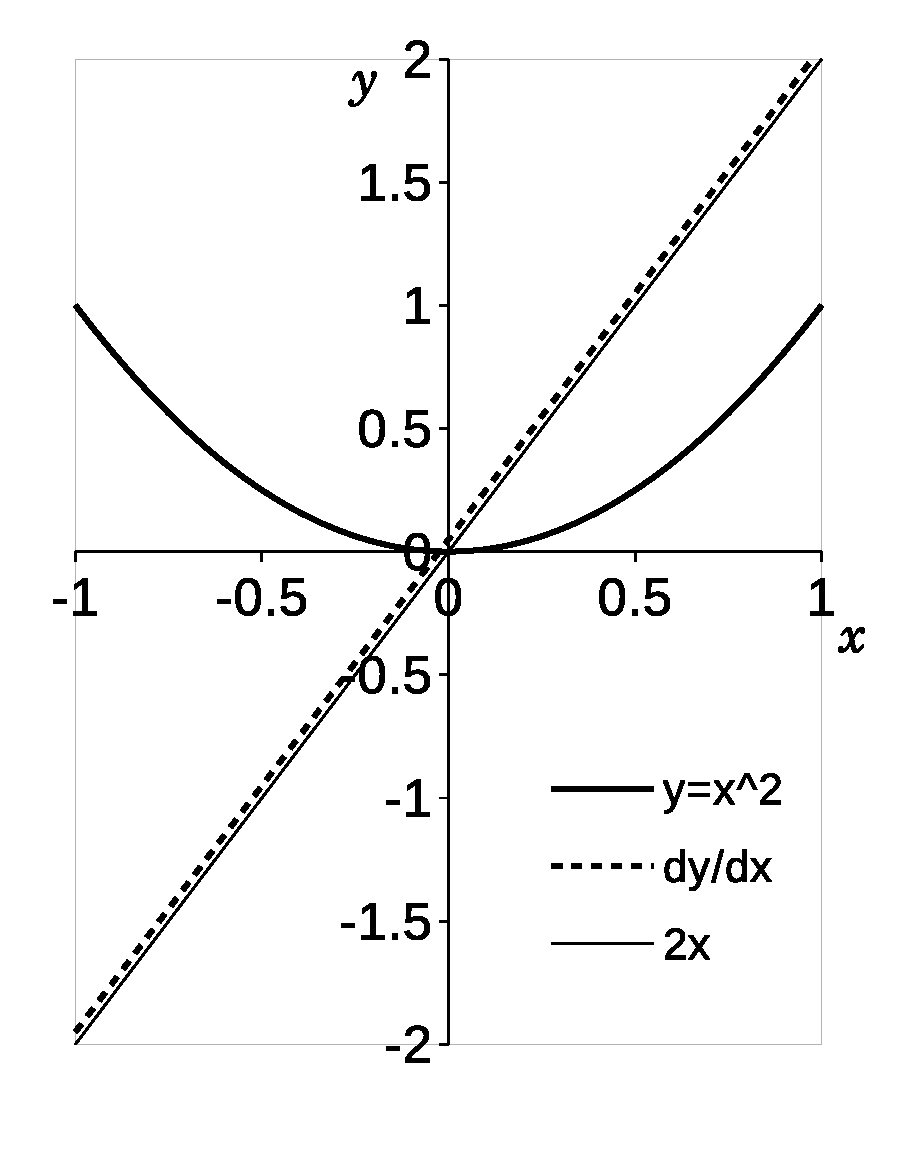
\includegraphics[width=4.7cm]{diffx2.eps}
    \caption{$y=x^2$とその数値微分($dy/dx$), そして$y=2x$。$x$の刻みは0.05。
数値微分と$y=2x$は, 刻みを小さくすればもっと近くなる。
例\ref{ex:x2deriv}の結論を数値微分でも確認できた!\label{fig:diffx2}}
\end{figure}
\hv


\section{グラフから導関数を直感的に作る}

導関数という概念を, グラフでもう少し直感的に考えてみよう。例として図\ref{fig:diff_graph}を
考える。ここには, ある関数$y=f(x)$と(上段), その導関数$y=f'(x)$ (下段)のそれぞれのグラフ
を上下に並べて描いてある。$y=f(x)$のグラフ上の点A, B, C, D, Eを考えよう。各点における
接線を, 点線で描いてある。これらの接線は, 点Aや点Eではほどんど水平だが, 点B, C, Dでは
右上がりである。特に, 点Cでの接線はかなり急な傾きを持っている。

従って, 「接線の傾き」という観点では, 点A, Eではほぼ0であり, 点B, Dでは「そこそこ」の大きさ, 
そして点Cで最も大きい。直感的には, 「接線の傾き」は微分係数のことなので, 各点での
「接線の傾き」をグラフにすると, ひとつの山型のグラフができる。それが下段の$y=f'(x)$である。

\begin{figure}[!h]
    \centering
    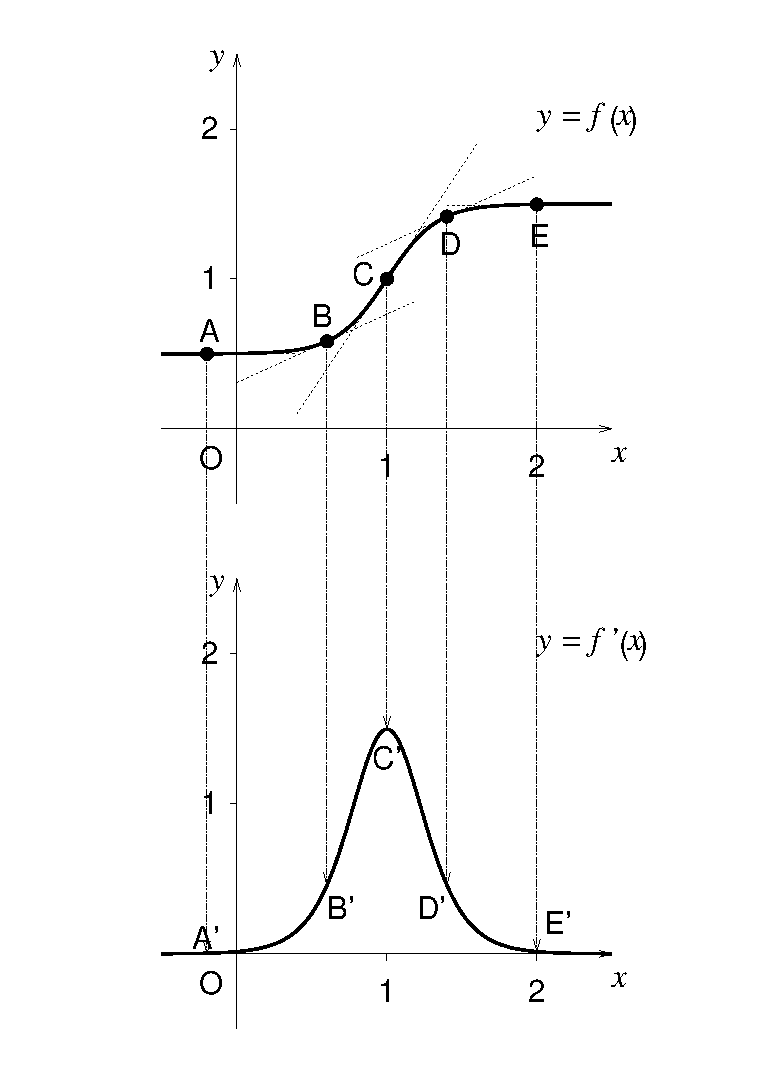
\includegraphics[width=8cm]{diff_graph.eps}
    \caption{関数$y=f(x)$とその導関数$y=f'(x)$。
$y=f(x)$のグラフは点C付近で傾き最大。従って, そのとき
導関数$y=f'(x)$は最大値をとる(点C')。\label{fig:diff_graph}}
\end{figure}

このように考えれば, 関数を数式として与えられなくても, その関数のグラフが与えられれば, 
その関数の導関数のグラフの概形を直感的に描くことができる。すなわち, 
関数上のいくつかの点での「接線の傾き」を考えて, それを別のグラフにプロットすれば
よいのだ。

\begin{q}\label{q:diff_graph_ex} 図\ref{fig:diff_graph_ex}に
に描かれた2つの関数について, それぞれ導関数の概形を重ねて描け。レポートを書くときは, 
レポート用紙にまずこのグラフを写しとってから, それに重ねて描け。
\end{q}
\begin{figure}[!h]
    \centering
    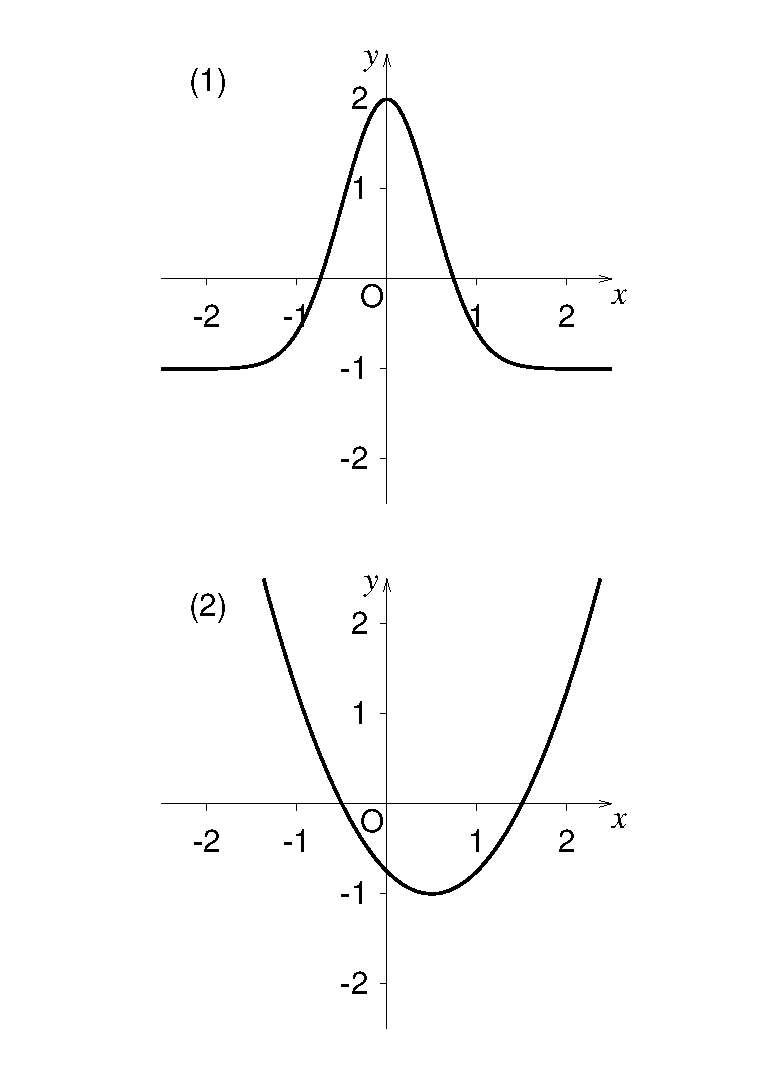
\includegraphics[width=8cm]{diff_graph_ex.eps}
    \caption{問\ref{q:diff_graph_ex}のグラフ。それぞれの導関数の概形を
描いてみよう。(1)のヒント: 左右の端と中央($x=0$)で, 接線の傾きは0になる。$x<0$では
右上がりなので接線の傾きはプラス。$0<x$では右下がりなので接線の傾きはマイナス。
\label{fig:diff_graph_ex}}
\end{figure}
\hv


\section{微分の公式}\label{sect:diff_formula}

実際に関数を微分するときは, 微分係数(導関数)の定義\eref{eq:define_dif}に
遡ってやることは少ない。複雑な関数の場合は前節でやったように数値微分を使うし, 
そうでなければ, 以下に示すような, いくつかの便利な定理(公式)を活用して
ちゃっちゃとやってしまうのだ。以下, $f(x), g(x)$を, 任意の(微分可能な)関数とする。
\hv

\begin{itembox}{微分の公式1: 足し算はバラせる}
\begin{eqnarray}
\{f(x)+g(x)\}'=f'(x)+g'(x)\label{eq:diff_form1}
\end{eqnarray}
\end{itembox}
証明: $F(x)=f(x)+g(x)$とおくと, 
\begin{eqnarray}
F(x+dx) & = & f(x+dx)+g(x+dx)\nonumber\\
               & = & f(x)+f'(x)dx+g(x)+g'(x)dx\nonumber\\
               & = & f(x)+g(x)+\{f'(x)+g'(x)\}dx\nonumber\\
               & = & F(x)+\{f'(x)+g'(x)\}dx
\end{eqnarray}
ここで, $dx$の係数に着目すると, 微分係数の定義から, $F'(x)=f'(x)+g'(x)$。\qed
\vv

\begin{exmpl}  $f(x)=x^2+2x$を微分しよう。公式1を使うと, 
\begin{eqnarray}
f'(x)=(x^2+2x)'=(x^2)'+(2x)'
\end{eqnarray}
となる。例\ref{ex:x2deriv}から, $(x^2)'=2x$であり,\eref{eq:diff_px+q}から, $(2x)'=2$である。従って, 
\begin{eqnarray}
f'(x)=2x+2
\end{eqnarray}
となる。(例おわり)\end{exmpl}
\hv

\begin{itembox}{微分の公式2: 定数倍は前に出せる}
$a$を定数として, 
\begin{eqnarray}
\{af(x)\}'=af'(x)\label{eq:diff_form2}
\end{eqnarray}
\end{itembox}
証明: $F(x)=af(x)$とおくと, 
\begin{eqnarray}
F(x+dx) & = & af(x+dx) = a\{f(x)+f'(x)dx\}\nonumber\\
               & = & af(x)+af'(x)dx\nonumber\\
               & = & F(x)+af'(x)dx
\end{eqnarray}
ここで, $dx$の係数に着目すると, 微分係数の定義から, $F'(x)=af'(x)$。\qed
\hv

微分の公式1と2のような性質は, 数列の和$\Sigma$にもあった
こと(P.\pageref{eq:sum_linear1})を覚えているだろうか? (線型性)\hv

\begin{exmpl}  $f(x)=3x^2$を微分しよう。公式2を使うと, 
\begin{eqnarray}
f'(x)=(3x^2)'=3(x^2)'
\end{eqnarray}
となる。例\ref{ex:x2deriv}から, $(x^2)'=2x$である。従って, 
\begin{eqnarray}
f'(x)=3(2x)=6x
\end{eqnarray}
となる。(例おわり)\end{exmpl}\

\begin{exmpl} 関数$f(x)=x^3+2x^2+3x+1$を微分しよう。
公式1, 公式2より, 
\begin{eqnarray}f'(x)=(x^3)'+2(x^2)'+3(x)'+(1)'\end{eqnarray}
ここで, 右辺の$(1)'$とは定数関数1(すべての$x$に対して定数1を対応させる関数)の微分であり, 
\eref{eq:diff_q}より, もちろん0である。$(x^3)'$や$(x^2)'$, $(x)'$に
\eref{eq:diff_x}を使うと, 
\begin{eqnarray}=3x^2+4x+3\end{eqnarray}
(例おわり)\end{exmpl}
\hv

%-----------

\begin{q}\label{q:diff_func0} 以下の関数を微分せよ:
\begin{enumerate}
\item $f(x)=x^2+x+1$
\item $f(x)=4x^2+5x+6$
\item $f(x)=3x^2+3x+4$
\item $f(x)=5/x$ (ヒント: 例\ref{ex:1overxderiv}を使う)
\item $f(x)=x-1/x$
\end{enumerate}\end{q}
\hv

\begin{itembox}{微分の公式3: 積の微分}
\begin{eqnarray}
\{f(x)g(x)\}'=f'(x)g(x)+f(x)g'(x)\label{eq:diff_form3}
\end{eqnarray}
\end{itembox}

証明: $F(x)=f(x)g(x)$とおくと, 
\begin{eqnarray*}
F(x+dx) & = & f(x+dx)g(x+dx)\\
               & = & \{f(x)+f'(x)dx\}\{g(x)+g'(x)dx\}\\
               & = & f(x)g(x)+f'(x)g(x)dx\\
               &   & +f(x)g'(x)dx+f'(x)g'(x)dx^2
\end{eqnarray*}
ここで, $dx^2$を無視し, さらに, $dx$の項を整理し, また, $f(x)g(x)$を$F(x)$で置き換えると, 
\begin{eqnarray*}F(x+dx)= F(x)+\{f'(x)g(x)+f(x)g'(x)\}dx\end{eqnarray*}
$dx$の係数に着目すると, 微分係数の定義から, 
\begin{eqnarray}F'(x)=f'(x)g(x)+f(x)g'(x)\end{eqnarray}
\qed
\hv

\begin{exmpl}  関数$F(x)=(x^2+2)(x^2+x+3)$を微分しよう。
$f(x)=x^2+2$, $g(x)=x^2+x+3$として, 公式3を使うと, 
\begin{eqnarray}
F'(x)&=&(x^2+2)'(x^2+x+3)+(x^2+2)(x^2+x+3)'\nonumber\\
     &=&2x(x^2+x+3)+(x^2+2)(2x+1)\nonumber\\
     &=&4x^3+3x^2+10x+2
\end{eqnarray}
となる。一方, 先に因数を展開してしまって, 
\begin{eqnarray}
F'(x)&=&(x^4+x^3+5x^2+2x+6)'\nonumber\\
     &=&(x^4)'+(x^3)'+5(x^2)'+2(x)'+(6)'\nonumber\\
     &=&4x^3+3x^2+10x+2
\end{eqnarray}
とすることもできる。どちらのやりかたでやっても, 答えは一致する。このように, 
数学は色んなやり方で正解に到達できるものなのだ。
(例おわり)\end{exmpl}
\hv

%-----------
\begin{q}\label{q:diff_func1} 以下の関数:
\begin{eqnarray}f(x)=(x^2+x+1)(x^2-x-2)\end{eqnarray}
について, 
\begin{enumerate}
\item 2つの関数: $x^2+x+1$と$x^2-x-2$の積とみなして, 積の微分の公式を使って微分せよ。
\item 因数を展開して(つまり掛け算を実行してカッコを外して)から微分し, 前小問の結果と一致することを確認せよ。
\end{enumerate}\end{q}
\vspace{0.3cm}

「関数$f(x)$」などの$(x)$を省略して書くことがよくある。式が単純になって
見やすいし覚えやすい。公式1, 2, 3は, それぞれ以下のようになる:
\begin{eqnarray}
(f+g)'&=&f'+g'\\
(af)'&=&af'\\
(fg)'&=&f'g+fg'
\end{eqnarray}

さて, 多くの学生がつまずくのが次の公式である。といっても, しっかり説明を
読めば難しくないはずだ。

\begin{itembox}{微分の公式4: 合成関数の微分}
\begin{eqnarray}
\{g(f(x))\}'=g'(f(x))f'(x)\label{eq:diff_form4}
\end{eqnarray}
注: ここで$g'(f(x))$は, $g(x)$の導関数$g'(x)$の$x$の部分に$f(x)$を代入したもの
であり, $g(f(x))$の導関数ではない。\end{itembox}

証明の前に例を示す:

\begin{exmpl}\label{exmpl:bibun_x213}  関数$(x^2+1)^3$を微分しよう。この関数を, 
「$g(x)=x^3$という関数の$x$の部分に, $f(x)=x^2+1$という関数を入れたもの」
とみなす。$g'(x)=3x^2$だから, 公式4より, 
\begin{eqnarray}
\{(x^2+1)^3\}'&=&\{(f(x))^3\}'=3(f(x))^2f'(x)\nonumber\\
               &=&3(x^2+1)^2\,\{(x^2+1)'\}=3(x^2+1)^2(2x)\nonumber\\
               &=&6x(x^2+1)^2\label{eq:diffexample9}
\end{eqnarray}
となる。これで完了としてよいのだが, ここではあえて\eref{eq:diffexample9}を展開すると, 
\begin{eqnarray}
6x^5+12x^3+6x\label{eq:diffexample91}
\end{eqnarray}
となる。一方, $(x^2+1)^3$を先に展開してから微分すると,
\begin{eqnarray}
\{(x^2+1)^3\}'&=&(x^6+3x^4+3x^2+1)'\nonumber\\
               &=&6x^5+12x^3+6x\label{eq:diffexample92}
\end{eqnarray}
となる。\eref{eq:diffexample91}, \eref{eq:diffexample92}は一致している
(つじつま合っている)。(例おわり)\end{exmpl}

この例は別に公式4を使わなくても, 式を展開してから
普通に微分すれば解けた。しかし, 次の例のように, 公式4がどうしても
必要になる場面もたくさんある:\mv

\begin{exmpl} 次の関数を微分しよう。
\begin{eqnarray}\frac{1}{2x^2+1}\end{eqnarray}
$f(x)=2x^2+1$, $g(x)=1/x$として, 
公式4を使おう。\eref{eq:dif_recipr}より$g'(x)=-1/x^2$である。従って, 
\begin{eqnarray}
\Bigl\{\frac{1}{2x^2+1}\Bigr\}'
&=&-\frac{1}{(f(x))^2}\times f'(x)\nonumber\\
&=&-\frac{1}{(2x^2+1)^2}\times(2x^2+1)'\nonumber\\
     &=&-\frac{4x}{(2x^2+1)^2}\label{eq:diffexample95}
\end{eqnarray}
となる。(例おわり)\end{exmpl}
\mv

実際には, こういうふうに$g(x)$や$f(x)$をわざわざ
作ったりしないで, 頭の中でまず$2x^2+1$をひとつの
変数とみなして全体を微分し, さらに$2x^2+1$を$x$で微分して掛け合わせ, 
いきなり\eref{eq:diffexample95}の最後の行を暗算で導出
できるようになるのが望ましい。最初は難しいかもしれないが, 慣れるまで練習しよう。\hv

では公式4を証明しよう: $F(x)=g(f(x))$とおくと, 
\begin{eqnarray}
F(x+dx) & = & g(f(x+dx))\nonumber\\
        & = & g\bigl(f(x)+f'(x)dx\bigr)\label{eq:dif_gosei1}
\end{eqnarray}
ここで, $dx$は0に限りなく近い微小量なので, それに$f'(x)$を掛けた数, すなわち$f'(x)dx$も, 
0に限りなく近い微小量とみなすことができる。そこで, 微分係数の定義\eref{eq:define_dif}
において, $f(x)$を$g(x)$とし, $x_0$を$f(x)$とし, $dx$を$f'(x)dx$とすれば, 
\begin{eqnarray}
g\bigl(f(x)+f'(x)dx\bigr)= g(f(x))+g'(f(x))\{f'(x)dx\}\nonumber\\\label{eq:dif_gosei2}
\end{eqnarray}
となる。右辺第一項の$g(f(x))$は, もちろん$F(x)$である。従って, \eref{eq:dif_gosei1}\eref{eq:dif_gosei2}より, 
\begin{eqnarray}
F(x+dx)=F(x)+g'(f(x))f'(x)dx\label{eq:dif_gosei3}
\end{eqnarray}
$dx$の係数に着目すると, 微分係数の定義から, \\
$F'(x)=g'(f(x))f'(x)$。\qed
\vv

この公式は, 一見, 複雑そうに見えるが, \eref{eq:define_dif25}のような書き方を使うと,
\begin{eqnarray}
\frac{dg}{dx}=\frac{dg}{df}\frac{df}{dx}\label{eq:diff_form45}
\end{eqnarray}
と表せる。右辺に現れる2つの微分の掛け算を, 形式的に, 微小量$dg$, $df$, $dx$の
分数の掛け算とみなせば, 右辺を約分したものが左辺になるだけだ。\mv

%-----------
\begin{q}\label{q:diff_func2} 以下の関数を, 合成関数の微分の公式を使って微分せよ:
\begin{enumerate}
\item $F(x)=(3x^2+2)^3$
\item $F(x)=(x^2+x+1)^3$
\item $F(x)=(x^5+x^4+x^3+x^2+x+1)^2$
\item $F(x)=(1+1/x)^2$
\end{enumerate}\end{q}
\mv


%-----------
\begin{q}\label{q:diff_func3} 関数$u(x)$の逆数であらわされる関数$1/u(x)$の導関数は, 
以下で与えられることを示せ\footnote{\eref{eq:difdiv0}, \eref{eq:difdiv}では関数$u(x)$の「$(x)$」を
省略して書いていることに注意せよ。}:
\begin{eqnarray}
\Bigl(\frac{1}{u}\Bigr)'=-\frac{u'}{u^2}\label{eq:difdiv0}
\end{eqnarray}\end{q}
ヒント: $g(x)=1/x$, $f(x)=u(x)$として公式4を使う。
\mv

%-----------
\begin{q}\label{q:diff_func4} 関数$v(x)$と$u(x)$の比で作られる関数$v(x)/u(x)$の導関数は, 以下で与えられることを示せ:
\begin{eqnarray}
\Bigl(\frac{v}{u}\Bigr)'=\frac{v'u-vu'}{u^2}\label{eq:difdiv}
\end{eqnarray}\end{q}
\mv

%-----------
\begin{q}\label{q:diff_func5} 以下の関数を微分せよ:
\begin{edaenumerate}
\item \begin{eqnarray*}f(x)=\frac{1}{1+x^2}\end{eqnarray*}
\item \begin{eqnarray*}f(x)=\frac{x}{1+x^2}\end{eqnarray*}
\end{edaenumerate}
ヒント: (1)では$u(x)=1+x^2$として\eref{eq:difdiv0}を使う。(2)では$u(x)=1+x^2$, $v(x)=x$と
して\eref{eq:difdiv}を使う。
\end{q}
\mv

\begin{exmpl}  $1/x^n$を微分してみよう($n$は1以上の整数の定数とする)。この関数は, 
\begin{eqnarray*}g(x)=x^n\,\,\,\text{と, }f(x)=\frac{1}{x}\end{eqnarray*}
の合成関数とみなせる。実際
\begin{eqnarray}g(f(x))=\Bigl(\frac{1}{x}\Bigr)^n=\frac{1}{x^n}\end{eqnarray}
となる。ところで,\eref{eq:diff_x}より$g'(x)=nx^{n-1}$であり, 例\ref{ex:1overxderiv}より$f'(x)=-1/x^2$だから, 
\eref{eq:diff_form4}より, 次式が成り立つ:
\begin{eqnarray}
\Bigl(\frac{1}{x^n}\Bigr)'&=&n\Bigl(\frac{1}{x}\Bigr)^{n-1}\Bigl(\frac{1}{x}\Bigr)'\nonumber\\
     &=&n\Bigl(\frac{1}{x}\Bigr)^{n-1}\Bigl(-\frac{1}{x^2}\Bigr)\nonumber\\
     &=&-\frac{n}{x^{n+1}}
\label{eq:xpowminusn1}\end{eqnarray}
\end{exmpl}

\eref{eq:xpowminusn1}は次のように書き換えられる。
\begin{eqnarray}(x^{-n})'=\,-n\,x^{-n-1}\label{eq:xpowminusn3}\end{eqnarray}
これは, \eref{eq:diff_x}で$n$を$-n$と置き換えたものに一致する。
もともと\eref{eq:diff_x}では, $n$を$1$以上の整数としたが, これで, 
定数$n$が負の整数のときも成り立つことがわかった。\hv

次に学ぶ公式は, 公式4の応用だ。これは\pref{eq:taisuu00}で
学んだ対数を微分したりするのに使う(その話は後の章に出てくる)。

\begin{itembox}{微分の公式5: 逆関数の微分}
$g(x)$を$f(x)$の逆関数とすると
\begin{eqnarray}
g'(x)=\frac{1}{f'(g(x))}\label{eq:diff_form5}
\end{eqnarray}
注: ここで$f'(g(x))$は, $f(x)$の導関数$f'(x)$に
$g(x)$を代入したものだ。$f(g(x))$の導関数ではない。
\end{itembox}
証明: 
%\begin{eqnarray}
%&&f(x)=y\label{eq:diff_form5_p1}\\
%&&f(x+dx)=y+dy\label{eq:diff_form5_p2}
%\end{eqnarray}
%とする。$dx, dy$はともに微小量である。逆関数の定義より, 
%\begin{eqnarray}
%&&x=g(y)\label{eq:diff_form5_p3}\\
%&&x+dx=g(y+dy)\label{eq:diff_form5_p5}
%\end{eqnarray}
%である。\eref{eq:diff_form5_p3}, \eref{eq:diff_form5_p5}より, 
%\begin{eqnarray}dx=g(y+dy)-g(y)\label{eq:diff_form5_p7}\end{eqnarray}
%である。さて, $f(x)$の導関数の定義式:
%\begin{eqnarray}f(x+dx) = f(x)+f'(x)dx\label{eq:diff_form5_p8}\end{eqnarray}を考える。左辺は\eref{eq:diff_form5_p2}より$y+dy$である。
%右辺第一項は\eref{eq:diff_form5_p1}より$y$である。右辺第二項の$dx$は\eref{eq:diff_form5_p7}で置き換えられる。すると\eref{eq:diff_form5_p8}は次式のように書き換えられる:
%\begin{eqnarray}y+dy = y + f'(g(y))\{g(y+dy)-g(y)\}\end{eqnarray}
%これを変形すると, 
%\begin{eqnarray}g(y+dy) = g(y) + \frac{1}{f'(g(y))}dy\end{eqnarray}
%ここで形式的に, $y$と$x$を入れ替え, $dy$と$dx$を入れ替えて, 
%\begin{eqnarray}g(x+dx) = g(x) + \frac{1}{f'(g(x))}dx\end{eqnarray}
%ここで$dx$の係数に着目すれば, 
%\begin{eqnarray}g'(x)=\frac{1}{f'(g(x))}\end{eqnarray}
%となり, \eref{eq:diff_form5}に一致する。\qed
%\hv

%別の証明:
合成関数の微分より, 
\begin{eqnarray}\{f(g(x))\}'= f'(g(x))g'(x)\label{eq:diff_fgxgx1}\end{eqnarray}
である。ところで, $g(x)$は$f(x)$の逆関数なので, \pref{eq:generaleq}の
\eref{eq:generaleq}より, 恒等的に$f(g(x))=x$である。従って, 
\begin{eqnarray}\{f(g(x))\}'=(x)'=1\label{eq:diff_fgxgx2}\end{eqnarray}
\eref{eq:diff_fgxgx1}と\eref{eq:diff_fgxgx2}より, 
\begin{eqnarray}f'(g(x))g'(x)=1\end{eqnarray}
この両辺を$f'(g(x))$で割れば, 
\begin{eqnarray}g'(x)=\frac{1}{f'(g(x))}\end{eqnarray}
となり, \eref{eq:diff_form5}に一致する。\qed
\hv
\begin{comment}
\begin{figure}[h]
    \centering
    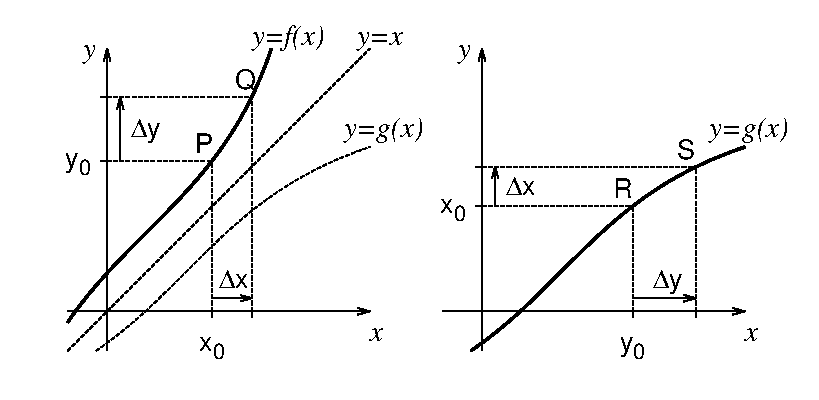
\includegraphics[width=8.5cm]{tan_atan.eps}
    \caption{関数$y=f(x)$と逆関数$y=g(x)$の微分}\label{fig:tan_atan}
\end{figure}
別の証明:
$y=f(x)$のグラフ上の2点:
\begin{eqnarray*}
\text{P: }&&(x_0, y_0)\\
\text{Q: }&&(x_0+\Delta x, y_0+\Delta y)
\end{eqnarray*}
において(\fref{fig:tan_atan}左), PとQが十分に近接していれば, 
\begin{eqnarray}
f'(x_0)\fallingdotseq\frac{\Delta y}{\Delta x}\label{eq:invdev1}
\end{eqnarray}
である。さて, $y=f(x)$のグラフを, $x$軸と$y$軸を入れ替えたら$y=g(x)$のグラフになる
のだから, 点Pや点Qの$x$座標と$y$座標を入れ替えた点
\begin{eqnarray*}
\text{R: }&&(y_0, x_0)\\
\text{S: }&&(y_0+\Delta y, x_0+\Delta x)
\end{eqnarray*}
は, 逆関数$g(x)$のグラフの上にある(\fref{fig:tan_atan}右)。RとSが十分に近接していれば, 
\begin{eqnarray}
g'(y_0)\fallingdotseq\frac{\Delta x}{\Delta y}\label{eq:invdev2}
\end{eqnarray}
である。\eref{eq:invdev1}, \eref{eq:invdev2}より, 
\begin{eqnarray}
g'(y_0)\fallingdotseq\frac{1}{\Delta y/\Delta x}\fallingdotseq\frac{1}{f'(x_0)}\label{eq:invdev3}
\end{eqnarray}
となる。$\Delta x$を0に近づける極限では右辺の$\fallingdotseq$は=になる。また, $f(x_0)=y_0$なので, 
$x_0=g(y_0)$。従って, \eref{eq:invdev3}は, 
\begin{eqnarray}
g'(y_0)=\frac{1}{f'(g(y_0))}\label{eq:invdev4}
\end{eqnarray}
となる。ここで$y_0$を改めて$x$と置きなおせば, 
\begin{eqnarray*}
g'(x)=\frac{1}{f'(g(x))}
\end{eqnarray*}
となり, \eref{eq:diff_form5}に一致する。\qed
\hv

この公\eref{eq:diff_form5}も, 一見, 複雑そうに見えるが, 以下の
ように考えれば, 実は単純である: 公\eref{eq:diff_form5}の$x$と$y$
を形式的に入れ替えれば, 
\begin{eqnarray}
g'(y)=\frac{1}{f'(g(y))}\label{eq:diff_form5c}
\end{eqnarray}
となる。ここで$x=g(y)$と置けば, $y=f(x)$だから, 
\begin{eqnarray}
&&g'(y)=\frac{dg}{dy}=\frac{dx}{dy}\label{eq:diff_form5c2}\\
&&f'(g(y))=f'(x)=\frac{df}{dx}=\frac{dy}{dx}\label{eq:diff_form5c4}
\end{eqnarray}
である。\eref{eq:diff_form5c}の左辺を\eref{eq:diff_form5c2}で, 右辺を\eref{eq:diff_form5c4}で書き換えれば, 
\begin{eqnarray}
\frac{dx}{dy}=\frac{1}{\frac{dy}{dx}}
\end{eqnarray}
と書ける。つまり, 逆関数の微分の公式は, 形式的には, 
微小量$dx$, $dy$の比の逆数をとっただけである。
そのことは, 上述のグラフを使った証明でも明らかだろう。\hv
\end{comment}

\begin{exmpl}  $f(x)=x^{1/n}$を微分してみよう。ただし$n$は1以上の整数とする。
$g(x)=x^n$とすると, $g(f(x))=x$だから, $g(x)$と$f(x)$は互いに逆関数。一方, $g'(x)=nx^{n-1}$である。
\eref{eq:diff_form5}(逆関数の微分)より, 
\begin{eqnarray}
f'(x)&=&\frac{1}{g'(f(x))}=\frac{1}{n(f(x))^{n-1}}=\frac{1}{n(x^{1/n})^{n-1}}\nonumber\\
&=&\frac{1}{nx^{(n-1)/n}}=\frac{1}{n}x^{-(n-1)/n}\nonumber\\
&=&\frac{1}{n}x^{(1-n)/n}=\frac{1}{n}x^{(1/n)-1}\label{eq:xpowfrc}
\end{eqnarray}
(例おわり)\end{exmpl}

\eref{eq:xpowfrc}は, \eref{eq:diff_x}で$n$を$1/n$と置き換えたものに一致する。
これで, \eref{eq:diff_x}は, 定数$n$が正の整数の逆数のときも成り立つことがわかった。

\eref{eq:diff_x}, \eref{eq:xpowminusn3}, \eref{eq:xpowfrc}からわかったように, 
定数$\alpha$が正の整数または負の整数または正の整数の逆数のとき, 
\begin{eqnarray}(x^{\alpha})'=\alpha x^{\alpha-1}\end{eqnarray}
が成り立つ。そのことと合成関数の微分の公式を使えば, $\alpha$が負の整数の逆数
のときや, 0以外の有理数(整数どうしの比であらわされる数)のときもこれが成り立つこと
が証明できる。実数は有理数の極限としてあらわされるので
\footnote{このあたりは高度な数学になるので, 詳細はわからなくてもよい。}, 有理数で成り立てば, 実数でも成り立つ。
従って, 以下の公式が成り立つ:\hv

\begin{itembox}{微分の公式6: べき関数の微分}
定数$\alpha$が0以外の実数であれば, 
\begin{eqnarray}
(x^{\alpha})'=\alpha x^{\alpha-1}\label{eq:diff_form6}
\end{eqnarray}
\end{itembox}

\begin{exmpl} もういちど関数$f(x)=1/x$を微分してみよう。$1/x=x^{-1}$だから, \eref{eq:diff_form6}
で$\alpha=-1$とすれば, 
\begin{eqnarray}
f'(x)=(x^{-1})'=-1\cdot x^{-2}=-\frac{1}{x^2}
\end{eqnarray}
これは式(\ref{eq:dif_recipr})と一致する。つじつまがあっている。(例おわり)\end{exmpl}

\begin{exmpl} $\sqrt{x}$を微分してみよう。
\begin{eqnarray}
(\sqrt{x})'=(x^{1/2})'=\frac{1}{2}\,x^{1/2-1}=\frac{1}{2}x^{-1/2}=\frac{1}{2\sqrt{x}}\nonumber\\
\end{eqnarray}
(例おわり)\end{exmpl}

%----------
\begin{q}\label{q:diff_pow} 公式6を使って, 以下の関数を微分せよ。
\begin{edaenumerate}<4>
\item \begin{eqnarray*}\frac{1}{x}\,\,\,\,\,\,\,\,\end{eqnarray*}
\item \begin{eqnarray*}\frac{1}{\sqrt{x}}\,\,\,\,\,\,\,\,\end{eqnarray*}
\item \begin{eqnarray*}x^{2/3}\,\,\,\,\,\,\,\,\end{eqnarray*}
\item \begin{eqnarray*}x^{-5}\,\,\,\,\,\,\,\,\end{eqnarray*}
\end{edaenumerate}\end{q}
\mv

%----------
\begin{q}\label{q:diff_theories1_5} 微分の公式1〜5を証明せよ。\end{q}
\mv

微分の計算は, とにかくたくさん練習して, 規則性を体に染み込ませよう。
微分の定義はとても大切だけど, 実際の関数を手計算で微分するときは, 
微分の定義よりもむしろ, これまで見てきたようないろいろな公式を
機械的に適用するのだ。\hv

\begin{exmpl}\label{exmpl:diff_sqrtx2p1} $\sqrt{x^2+1}$を微分してみよう。$g(x)=\sqrt{x}$と
$f(x)=x^2+1$の合成関数$g(f(x))$とみなして, 
\begin{eqnarray}
(\sqrt{x^2+1})'&=&\frac{1}{2\sqrt{x^2+1}}\times(x^2+1)'\nonumber\\
                &=&\frac{2x}{2\sqrt{x^2+1}}=\frac{x}{\sqrt{x^2+1}}\label{eq:exmpl_diff_23}
\end{eqnarray}
(例おわり)\end{exmpl}

\begin{exmpl} $x\sqrt{x^2+1}$を微分してみよう。
\begin{eqnarray}
(x\sqrt{x^2+1})'&=&x'\sqrt{x^2+1}+x(\sqrt{x^2+1})'\nonumber\\
                &=&\sqrt{x^2+1}+x\times\frac{x}{\sqrt{x^2+1}}\nonumber\\
                &=&\sqrt{x^2+1}+\frac{x^2}{\sqrt{x^2+1}}
\end{eqnarray}
最初の変形では積の微分(公式3)を使った($x$と$\sqrt{x^2+1}$の積)。それ以降は\eref{eq:exmpl_diff_23}の
結果を使った。(例おわり)\end{exmpl}
\mv

\begin{freqmiss}{\small\textgt{微分記号を省略し, 微分する前の関数と微分した
後の関数をイコールで結んでしまう。例えば, $(x^2+x)'=2x+1$と
書くべきところを, $x^2+x=2x+1$と書いてしまう。}}\end{freqmiss}
\mv

%----------
\begin{q}\label{q:diff_func8} 微分の公式を駆使して, 以下の関数を微分せよ:
\begin{edaenumerate}<3>
\item \begin{eqnarray*}\sqrt{2x+3}\,\,\,\,\,\,\,\,\,\,\,\,\,\,\,\end{eqnarray*}
\item \begin{eqnarray*}\sqrt{1-x^2}\,\,\,\,\,\,\,\,\,\,\,\,\,\,\,\end{eqnarray*}
\item \begin{eqnarray*}x^2\sqrt{1+x^2}\,\,\,\,\,\,\,\,\,\,\,\,\,\,\,\end{eqnarray*}
\item \begin{eqnarray*}\frac{1}{\sqrt{1+x^2}}\,\,\,\,\,\,\,\,\,\,\,\,\,\,\,\end{eqnarray*}
\item \begin{eqnarray*}\frac{1}{1+\sqrt{x}}\,\,\,\,\,\,\,\,\,\,\,\,\,\,\,\end{eqnarray*}
\item \begin{eqnarray*}\sqrt{1+\frac{1}{x}}\,\,\,\,\,\,\,\,\,\,\,\,\,\,\,\end{eqnarray*}
\item \begin{eqnarray*}\frac{x-1}{x+1}\,\,\,\,\,\,\,\,\,\,\,\,\,\,\,\end{eqnarray*}
\item \begin{eqnarray*}\frac{1}{1+\frac{1}{x}}\,\,\,\,\,\,\,\,\,\,\,\,\,\,\,\end{eqnarray*}
\end{edaenumerate}\end{q}
\vv



\section{線型近似}

\eref{eq:define_dif_Delta}で述べたように, 関数$f(x)$の, $x=x_0$における微分係数$f'(x_0)$は,
\begin{equation}
f(x_0+\Delta x) \fallingdotseq f(x_0) + f'(x_0) \Delta x
\end{equation}
を満たす。$\Delta x$が0に近ければ近いほど, 近似等号"$\fallingdotseq$"は等号"$=$"に
近づくのだが, たとえ有限小の$\Delta x$についても$f(x_0+\Delta x)$を, 
この右辺の式で置き換え, ざっくりと近似することがよくある。
これを関数の\underline{線型近似} \index{せんけいきんじ@線型近似} (一次近似
\index{いちじきんじ@一次近似})という。要するに, 関数を一次式で近似するのだ。
グラフで言えば, 曲線を, その接線で近似するのだ。

\begin{faq}{\small\textgt{それって, 数値微分の考え方に似てません?}
... そうです。というより, 数値微分は, 線型近似の考え方を使っているのです。}\end{faq}

線型近似は誤差が出てしまうが, 多少の誤差はOKという状況で式や
計算を単純化したいときにとても便利である。

特に, $x_0=0$とし, 0に近い範囲でしか$x$を考えないという前提で, $\Delta x$を$x$と置き換えることで, 
\begin{eqnarray}
f(x) \fallingdotseq f(0)+f'(0)x\label{eq:linear_approx00}
\end{eqnarray}
となる。実用上は, このタイプの近似式が, よく使われる。
では実際に線型近似をやってみよう。\mv

\begin{exmpl} $\,\,\,\,\,f(x)=\sqrt{1+x}$ を線型近似する:\\
$f'(x)=1/(2\sqrt{1+x})$なので, $f(0)=1, f'(0)=1/2$。これを\eref{eq:linear_approx00}
に入れると, $x=0$付近で
\begin{eqnarray}
\sqrt{1+x}\fallingdotseq 1+\frac{x}{2}\label{eq:linear_approx01}
\end{eqnarray}
となる。試しに, 実際にいくつかの値を計算してみよう。

$\sqrt{1.1}=1.04880...$だが, \eref{eq:linear_approx01}より, 
$\sqrt{1.1}=\sqrt{1+0.1}\fallingdotseq1+0.1/2=1.05$。

$\sqrt{1.01}=1.004987...$だが, \eref{eq:linear_approx01}より, 
$\sqrt{1.01}=\sqrt{1+0.01}\fallingdotseq1+0.01/2=1.005$。
(例おわり)\end{exmpl}
\mv

\begin{q}\label{q:univ_lin_approx0} $x=0$付近で, 以下の式が成り立つことを示せ(ただし$a$は任意の実数)。
\begin{eqnarray}
(1+x)^a\fallingdotseq1+ax\label{eq:linear_approx02}
\end{eqnarray}\end{q}

\eref{eq:linear_approx02}の形の線型近似はとてもよく使われる。

\begin{q}\label{q:univ_lin_approx2} 以下の関数を, $x=0$付近で線型近似せよ:
\begin{edaenumerate}<3>
\item $1/(1+x)$
\item $1/(1-x)$
\item $1/\sqrt {1+x}$
\end{edaenumerate}\end{q}
\mv

\eref{eq:linear_approx02}を利用すると, 多くの計算を(近似的にだが)簡単にできる。\mv

\begin{exmpl} $\,\,\,\,\,(1.01)^{10}$の近似値を求めよう。
これがもし$1^{10}$なら楽である。そこで, $1.01=1+0.01$というふうに考える: 
$(1+0.01)^{10} \fallingdotseq 1+10\times0.01 = 1.1$\\
正確には$(1.01)^{10}=1.1046\cdots$であり, 有効数字3桁まで合っている。
\end{exmpl}

\begin{exmpl} $\,\,\,\,\,\sqrt{26}$の近似値を求めよう。2乗して
26に近い数は何かな?と考えると, $5^2=25$である。そこで, 
$26=25+1$と考える。
\begin{eqnarray*}
\sqrt{26}&&=\sqrt{25+1}=\sqrt{25\Bigl(1+\frac{1}{25}\Bigr)}=5\sqrt{1+\frac{1}{25}}\\
&&\fallingdotseq5\Bigl(1+\frac{1}{50}\Bigr)=5.1
\end{eqnarray*}
正確には$\sqrt{26}=5.0990\cdots$であり, 有効数字3桁まで合っている(4桁目を四捨五入
すると一致する)。この式展開で, 25を先に$\sqrt{\quad}$の外に追い出し, $\sqrt{\quad}$の
中を$1+1/25$の形にしたところがコツなのだ。$1/25$は0にそこそこ近いので, 
\eref{eq:linear_approx02}が使えたのだ。このように, まずざっくり簡単な
近似値(この場合は5)を勘で見つけることが大事。それをもとに, 線型近似で精度を
上げるのだ。(例おわり)\end{exmpl}
\mv

\begin{q}\label{q:univ_lin_approx4} 線型近似を利用して, 以下の値を近似的に求めよ(電卓を使わないで筆算で。できれば暗算で!):
\begin{enumerate}
\item $(0.99)^{10}$ (正確には$0.9043\cdots$となる)
\item $10^{1/3}$ (正確には$2.1544\cdots$となる)
\end{enumerate}\end{q}
\mv


\section{高階導関数}

ところで, 関数$f(x)$を, 2回続けて微分することを考えよう。それを, \underline{2階微分}とか
\underline{2階導関数} (「回」ではなく「階」という字を使う)と呼び, $f''(x)$と書く(定義)。
2階導関数$f''(x)$は, \eref{eq:define_dif45}の書き方で書けば, 
\begin{eqnarray}
\frac{d}{dx}\Bigl(\frac{d}{dx}f(x)\Bigr)
\end{eqnarray}
とも書けるので, 形式的に縮めて, 
\begin{eqnarray*}
\frac{d^2}{dx^2}f(x)\quad\text{とか,}\quad 
\frac{d^2f}{dx^2}(x)\quad\text{とか,}\quad 
\frac{d^2f}{dx^2}
\end{eqnarray*}
と書くこともある。分母と分子で「2乗」のつく位置が異なることに注意。

これと同様に考えて, 「3階導関数」「4階導関数」...「$n$階導関数」など($n$は1以上の整数)も
考えることができ, それらはまとめて\underline{高階導関数} \index{こうかいどうかんすう@高階導関数}と呼び, 
\begin{eqnarray}
&&f^{(n)}(x)\label{eq:diff_mult_def1}\\
&&\frac{d^n}{dx^n}f(x)\label{eq:diff_mult_def2}\\
&&\frac{d^nf}{dx^n}(x)\label{eq:diff_mult_def3}\\
&&\frac{d^nf}{dx^n}\label{eq:diff_mult_def4}
\end{eqnarray}
などと書く。独立変数$x$やその値が文脈上, 明らかであれば, \eref{eq:diff_mult_def4}のように, 
$(x)$は省略してもかまわない。\eref{eq:diff_mult_def1}については, $n$個の
ダッシュ「$'$」を書きたいところだが, $f''''''(x)$とか書くのは格好が
悪いので, 3階以上になったら, $(3)$とか$(n)$というふうに書く。\hv

%----------
\begin{q}\label{q:diff_func9} 以下の関数について, $f'(x)$, $f''(x)$, $f^{(3)}(x)$をそれぞれ求めよ。
\begin{edaenumerate}
\item \begin{eqnarray*}f(x)=x^5+2x^3\,\,\,\,\,\,\,\,\,\,\end{eqnarray*}
\item \begin{eqnarray*}f(x)=\frac{1}{1-x}\,\,\,\,\,\,\,\,\,\,\end{eqnarray*}
\end{edaenumerate}\end{q} 
\mv

\begin{faq}{\small\textgt{$d^2x/dt^2$の,$dt^2$や
$d^2x$はどういう状態?} ... 
既に述べたように, $dt^2$は$dt$かける$dt$です。
$d^2x$は, $t$が2段階で変化するときの「$x$の変化の変化」
と思えばよろしい。つまり, $t$が$t+dt$に変化した時の$dx$と, 
$t$が$t+dt$から$t+2dt$に変化した時の$dx$との差(後者引く前者)
が$d^2x$です。丁寧に書くと, $d(dx)$です。$dx$自体が微小量
だから, 微小量どうしの差はすごく小さい微小量になるという
ことが直感できるでしょう。$dt^2$や$d^2x$を「2次の微小量」
と言います。2次の微小量は$dt$や$dx$という1次の微小量
よりはるかに小さいので, 普通, 無視します(0とみなします)
が, この場合は, 2次の微小量どうしの比を考えているので, 
無視できないのです。

ところで, 高校で, $dx/dt$はそれ全体でひとつの記号
であり, 「$dx$わる$dt$」ではない, と習った人も
いるでしょう。厳密な数学はそのような立場です。しかし, 
生物資源学類が関わる多くの応用的な学問では, 
$dx/dt$を「$dx$わる$dt$」と考えてほとんど差し支えないし, 
その方が理解も応用もしやすいので, この授業ではその立場を
とります。}\end{faq}


\section{微分ができない場合}

ここまで読んで, 君は, どんな関数でも微分できるような気がしているかも
しれない。でも, 世の中には微分ができない(導関数や微分係数が存在しない)場合
もたくさんある。

\begin{exmpl}\label{ex:Nodif_1/x} 以下の関数
\begin{eqnarray}f(x)=\frac{1}{x}\end{eqnarray}
は, $x=0$以外では微分できて, 導関数は$f'(x)=-1/x^2$だ。では$x=0$では微分
できるだろうか? そもそも微分の定義である\eref{eq:define_dif}や
\eref{eq:define_dif2}に戻ると, 微分を考えるには$f(x_0)$の値が必要だ。
今は$x_0=0$を考えているので$f(0)$が必要。でもこの関数に$f(0)$は
存在しない(0での割り算は禁じ手である。$1/0=\infty$だと思っている
人もいるだろうが, $\infty$というのは数ではないのだ)。
なので, この関数は$x=0$では微分できない。(例おわり)
\end{exmpl}

この例\ref{ex:Nodif_1/x}では, 微分したい位置でそもそも関数の値が定まって
いなかった。そういう場合, 微分はできない。分数で表される関数で分母が0
になるときにこのような状況になることが多い。

\begin{exmpl}\label{ex:Nodif_|x|} 以下の関数
\begin{eqnarray}f(x)=|x|\label{eq:f(x)=|x|}\end{eqnarray}
の微分を考えよう。これは, 
\begin{eqnarray*}
f(x)=\begin{cases}
-x\,\,\,\,\,\,\,\,\,\,(x<0\text{のとき})\\
x\,\,\,\,\,\,\,\,\,\,\,\,\,(0\leq x\text{のとき})
\end{cases}\end{eqnarray*}
ということだ。従って, 導関数は
\begin{eqnarray}
f'(x)=\begin{cases}
-1\,\,\,\,\,\,\,\,\,\,(x<0\text{のとき})\\
1\,\,\,\,\,\,\,\,\,\,\,\,\,(0\leq x\text{のとき})
\end{cases}\label{eq:|x|'2}\end{eqnarray}
だと思うかもしれない。これはおおむね正しいが, \textgt{$x=0$のところで間違っているのだ}。
微分の定義である\eref{eq:define_dif}に戻ってみよう(\eref{eq:define_dif2}に戻っても
結論は同じ)。$x_0=0$とすれば, \eref{eq:define_dif}は
\begin{eqnarray}f(0+dx) = f(0)+f'(0)dx\label{eq:|x|'3}\end{eqnarray}
となる。ここで\eref{eq:f(x)=|x|}より, $f(0)=0$だから, \eref{eq:|x|'3}は
\begin{eqnarray}f(dx) = f'(0)dx\label{eq:|x|'4}\end{eqnarray}
となる。もし, \eref{eq:|x|'2}が正しければ, $f'(0)=1$となり, 従って\eref{eq:|x|'4}は
\begin{eqnarray}f(dx) = dx\label{eq:|x|'5}\end{eqnarray}
となるはず。ところが$dx$は0に近い任意の微小量なので, $dx<0$となる場合もあるだろう。
その場合, \eref{eq:|x|'5}から, $f(dx)<0$となる。ところが\eref{eq:f(x)=|x|}より, 
この関数は決して負の値をとることはあり得ない。従って矛盾する。従って, \eref{eq:|x|'2}は
$x=0$で正しくない\footnote{このような論法を「背理法」という。第\ref{chapt_logic}章参照。}。
同様に考えれば, $f'(0)$をどのような値にしても矛盾が生じることがわかるだろう。
従って, $f'(0)$は存在しない, すなわちこの関数は$x=0$では微分できない。(例おわり)
\end{exmpl}

この例\ref{ex:Nodif_|x|}で出てきた\eref{eq:f(x)=|x|}のグラフを図\ref{fig:abs_x}に示す。
微分したい位置($x=0$)で, グラフが尖っている。詳細は省くが, 一般に, グラフが尖っている
箇所では, 関数は微分不可能である。式に絶対値記号が入っていて, 絶対値記号の内側が0
になるときにこういう状況になることが多い
\footnote{ただしそうでないときもある。$f(x)=|x|^3$は$x=0$で絶対値記号内が0になるが, 
$x=0$で微分可能である。}。
\begin{figure}[h]
    \centering
    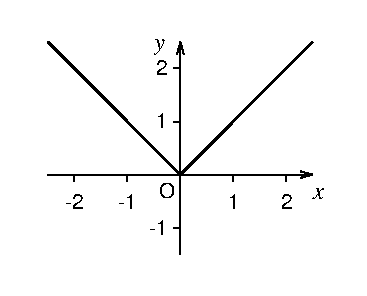
\includegraphics[width=5cm]{abs_x.eps}
    \caption{関数$y=|x|$のグラフ。$x=0$で微分不可能(尖っている)。}\label{fig:abs_x}
\end{figure}

\begin{exmpl}\label{ex:Nodif_01} 以下の関数
\begin{eqnarray}
f(x)=\begin{cases}
0\,\,\,\,\,\,\,\,\,\,(x<0\text{のとき})\\
1\,\,\,\,\,\,\,\,\,\,\,(0\leq x\text{のとき})
\end{cases}\label{eq:01'1}\end{eqnarray}
の微分を考えよう。定数関数の微分は0だから, 
\begin{eqnarray}
f'(x)=\begin{cases}
0\,\,\,\,\,\,\,\,\,\,(x<0\text{のとき})\\
0\,\,\,\,\,\,\,\,\,\,\,(0\leq x\text{のとき})
\end{cases}\label{eq:01'2}\end{eqnarray}
つまり, $f'(x)=0$のように思うかもしれない。これも, おおむね正しいが, 
\textgt{$x=0$のところで間違っているのだ!} 再び微分の定義である\eref{eq:define_dif}
に戻って考えてみよう。$x_0=0$, $f(x_0)=f(0)=1$とすれば, \eref{eq:define_dif}は
\begin{eqnarray}f(dx) = 1+f'(0)dx\label{eq:01'4}\end{eqnarray}
となる。もし, \eref{eq:01'2}が正しければ, $f'(0)=0$となり, 従って\eref{eq:01'4}は
\begin{eqnarray}f(dx) = 1\label{eq:01'5}\end{eqnarray}
となるはずだ。ところが$dx$は0に近い任意の微小量なので, $dx<0$となる場合もあるだろう。
その場合, \eref{eq:01'1}より, $f(dx)=0$となるはずで, これは\eref{eq:01'5}
に矛盾する。従って, $f'(0)=0$は$x=0$では成り立たない。実は, $f'(0)$にどのような
値を与えても, これらのつじつまを合わせることはできないのだ。(例おわり)
\end{exmpl}

\eref{eq:01'1}のグラフを図\ref{fig:step_func01}に示す。$x=0$でグラフがつながって
いない。詳細は省くが, 一般に, グラフがつながっていない\footnote{グラフがつながっていない, 
ということはどういうことかを, 数学的に定義するのは, 実は簡単なことでは無い。}
ようなところでは, 関数は微分できない。

\begin{figure}[h]
    \centering
    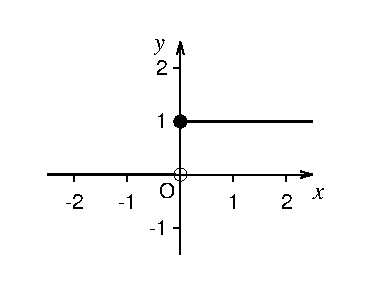
\includegraphics[width=5cm]{step_func01.eps}
    \caption{\eref{eq:01'1}の$y=f(x)$のグラフ。$x=0$で微分不可能(つながっていない)。}\label{fig:step_func01}
\end{figure}



\begin{exmpl}\label{ex:Nodif_xpow1/3} 以下の関数
\begin{eqnarray*}
f(x)=x^{1/3}
\end{eqnarray*}
の微分を考えよう。機械的に導関数を計算すると, 
\begin{eqnarray}f'(x)=\frac{1}{3x^{2/3}}\label{eq:xpow1/3'}\end{eqnarray}
となる。これは正しいのだが, この式では$x=0$での値が定まらない。つまり, この関数
は$f'(0)$を持たない。(例おわり)
\end{exmpl}

この例\ref{ex:Nodif_xpow1/3}では, 微分したい位置($x=0$)で, 関数の値は定まるが
導関数の値が定まらない($\infty$になってしまう)。グラフ(図\ref{fig:xpow1_3})
を見ると, $x=0$での傾きが無限大(接線が$x$軸に垂直)になりそうだ。詳細は省くが, 
グラフが垂直に立つようなところでは, 関数は微分できない。

\begin{figure}[h]
    \centering
    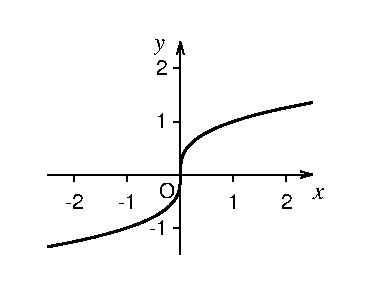
\includegraphics[width=5cm]{xpow1_3.eps}
    \caption{$y=x^{1/3}$のグラフ。$x=0$で微分不可能(傾きが$\infty$になる)。}\label{fig:xpow1_3}
\end{figure}

では, どのような場合なら微分可能なのだろうか? 数学的には, \eref{eq:define_dif}や
\eref{eq:define_dif2}によって$f'$が一意的に定義できる場合, 微分可能である。とは
いえ, いちいち\eref{eq:define_dif}や\eref{eq:define_dif2}に戻るのは大変だ。
さしあたって実用的には, 場合分けや絶対値記号が無く, 導関数の式を導くことができ, 
微分したい位置の$x$の値をもとの関数と導関数の両方に代入してそれぞれ値が定まる
ようならば, ほとんどの場合で微分できると思ってよい。
\vv




\section{速度・加速度} \label{secvelocity_and_acceleration}

さて, 微分は物理学で非常によく使われる。そもそも, 微分という概念は物理学上の必要
に迫られて発明されたのだ(それが今では, 化学・生物学・経済学・統計学等の広範な
学問に不可欠な道具になっている)。物理学で最初に出てくる微分は, 速度や加速度という考え方
である。それを学ぶために, まず準備として, いくつかの言葉を確認しておこう:
 
いま, $x$軸上を移動する点Pがあるとする。時刻$t$のときのPの位置($x$座標)を$x(t)$とする。
ある時刻$t_0$ではPは$x(t_0)$にあり, 別の時刻$t_1$ではPは$x(t_1)$にある。

2つの時刻の差, すなわち$t_1-t_0$を「時刻差」という\footnote{実際は「時刻差」という
言葉はめったに使わないが, ここでは時刻や時間と区別するために導入する。}。
$t_1>t_0$なら時刻差$t_1-t_0$は正の値をとるし, $t_1<t_0$なら時刻差$t_1-t_0$は負の値をとる。
時刻差$t_1-t_0$の絶対値, すなわち$|t_1-t_0|$を「時間」という。時間は常に0以上の値をとる。

2つの位置の差を変位(displacement)\index{へんい@変位}という。
今の場合, $x(t_1)-x(t_0)$が変位である。$x(t_1)>x(t_0)$なら変位は
正の値をとるし, $x(t_1)<x(t_0)$なら変位は負の値をとる。変位の絶対値
を「距離」(distance)\index{きょり@距離}という。今の場合, $|x(t_1)-x(t_0)|$が距離である。
当然ながら, 距離は常に0以上の値をとる。

まとめると, 
\begin{itemize}
\item $t$ ... 時刻
\item $t_1-t_0$ ... 時刻差 (時刻の差)
\item $|t_1-t_0|$ ... 時間 (時刻差の絶対値)
\item $x(t)$ ... 位置
\item $x(t_1)-x(t_0)$ ... 変位 (位置の差)
\item $|x(t_1)-x(t_0)|$ ... 距離 (変位の絶対値)
\end{itemize}
である。

さて, 「時刻$t_0$から$t_1$の間のPの平均速度$\overline{v}$」を, 次式で定義する:
\begin{eqnarray}\overline{v} :=\frac{x(t_1)-x(t_0)}{t_1-t_0}\label{eq:veloc_mean_def}\end{eqnarray}
すなわち, 平均速度とは変位を時刻差で割ったものだ。
\eref{eq:veloc_mean_def}で, もし時刻差が正で変位が負ならば, 
平均速度は負の値になる。このとき, Pは$x$軸の負の向きに進んでいる。
このように, 平均速度の正負は移動の向きを表す。

さて, \eref{eq:veloc_mean_def}で定義した「平均速度」は, 
時刻$t_0$と時刻$t_1$の間で物体の運動が勢いを増したり減らしたり, 
刻々と変化するような様子を表現できない。そのような細かな変化も表現する
には, 時刻$t_0$と時刻$t_1$の間をできるだけ短くして表現しなければならない。そこで, 
\eref{eq:veloc_mean_def}の$t_1$が, 限りなく$t_0$に近い場合(極限)
を考えよう。そのような極限は, 次式のようになる:
\begin{eqnarray}v(t_0):=\lim_{t_1\rightarrow t_0}\frac{x(t_1)-x(t_0)}{t_1-t_0}\label{eq:veloc_def0}\end{eqnarray}
あるいは$t_1-t_0=\Delta t$と書いて, 
\begin{eqnarray}v(t_0):=\lim_{\Delta t\rightarrow 0}\frac{x(t_0+\Delta t)-x(t_0)}{\Delta t}\label{eq:veloc_def1}\end{eqnarray}
と書く。この式を\eref{eq:define_dif2}と比べてみるとわかるように, これは
$x(t)$という関数の, $t=t_0$での微分係数である。これを「時刻$t_0$で
の\underline{速度} \index{そくど@速度}(velocity)」と言う。要するに
速度とは位置を時刻で微分したものである(定義)。このように定義した速度を, 
上述の「平均速度」と区別するためにわざわざ「瞬間の速度」と言うこともある。

時刻$t$における速度$v(t)$は, 定義より, $x'(t)$と書ける。物理学では, 
$x'(t)$のことを$\dot{x}$と表すこともある(上付きのドットが「時刻による微分」
を表すのだ)。つまり,
\begin{eqnarray}v(t)=\frac{dx}{dt}=x'(t)=\dot{x}\label{eq:veloc_def2}\end{eqnarray}
である。このように, 同じことをいろんな記法で表すことがある。

さて, 平均速度の正負が運動の方向を表したように, (瞬間の)速度にも正負が
あり, それは運動の方向を表す。

ここで, 速度の絶対値のことを\underline{速さ} (speed)と呼ぶ(定義)。
例えば\eref{eq:veloc_mean_def}の左辺と右辺のそれぞれ絶対値をとると, 
\begin{eqnarray}|\overline{v}|=\frac{|x(t_1)-x(t_0)|}{|t_1-t_0|}\label{eq:veloc_mean_def_abs}\end{eqnarray}
となる。これを平均速さという。
右辺の$|x(t_1)-x(t_0)|$は距離, $|t_1-t_0|$は時間なので, 
\eref{eq:veloc_mean_def_abs}は, \\
  「平均速さ=距離÷時間」\\
となる。ところが小学校では\\
  「速さ=距離÷時間」\\
と習った。つまり, 小学校で習った
「速さ」は, 正確に言うと「平均速さ」だったのだ。 
\eref{eq:veloc_mean_def_abs}で$t_1$を$t_0$に近づける極限は, 
(瞬間の)速度の絶対値であり, それを(瞬間の)速さという。

「速さ」は「速度」の大きさ(絶対値)なので, 必ず
0以上の値である。負の値をとることはない。つまり速さには
「向き」の概念が無い。逆に言えば, 速さと向きをセット
にした概念が速度である。\hv

\begin{freqmiss}{\small\textgt{
「速度は\textgt{距離}を時刻で微分したものである」
「速度は位置を微分したものである」などと言ってしまう} ... 
前者は, 距離ではなくて位置。後者は間違いではありませんが, どういう量
について(この場合は時刻)微分するのかもきちんと言わねばなりません。}
\end{freqmiss}

\begin{q}\label{q:diff_def}  
\begin{enumerate}
\item 平均速度と速度はどう違うか?
\item 速度と速さはどう違うか?
\item 速度と速さはぞれぞれどのような英語単語で表現されるか?
\item 「速度とは距離を時刻で微分したものだ」という発言はどこが間違っているか?
\item 「速度とは位置を微分したものだ」という発言はどこが間違っているか?
\end{enumerate}\end{q}
\hv

\eref{eq:define_dif}, \eref{eq:veloc_def2}より, 次式のようにも書ける:
\begin{eqnarray}
x(t+dt) = x(t) + v(t)dt\label{eq:xtdtxtvtdt}
\end{eqnarray}
ここで$dt$は微小な時刻差である。この\eref{eq:xtdtxtvtdt}によれば, 
$dt$だけ時刻が変化したときの位置(つまり$x(t+dt)$)は, 現在の位置(つまり$x(t)$)
から, $v(t)dt$だけ変化する(速度も, 時刻とともに変わるかもしれないが, 
$t$と$t+dt$の間では,ほとんど一定とみなすことができるだろう。というより
むしろ, 速度がほぼ一定とみなせるくらいに短い$dt$を考える)。つまり, 時刻差
が微小な場合は, 変位は速度と時刻差の積に等しい。それは, \eref{eq:xtdtxtvtdt}を
\begin{eqnarray}
x(t+dt)-x(t) = v(t)dt\label{eq:xtdtxtvtdt2}
\end{eqnarray}
と変形すれば, より明らかだろう。
ここで, \eref{eq:xtdtxtvtdt2}について両辺の絶対値をとると, 
\begin{eqnarray}
|x(t+dt)-x(t)| = |v(t)||dt|\label{eq:xtdtxtvtdt3}
\end{eqnarray}
となる。左辺は距離, 右辺は速さと時間の積である(速度の絶対値を「速さ」
というのだから, $|v(t)|$が「速さ」である)。これは, 小学校で習った, 
\begin{eqnarray}\text{距離}=\text{速さ}\times\text{時間}\end{eqnarray}
と整合的である。\hv

速度を時刻で微分したものを\underline{加速度} (acceleration)\index{かそくど@加速度}と言う(定義)。
すなわち, 時刻$t$における加速度$a(t)$とは, 
\begin{eqnarray}a(t)=v'(t)\label{eq:ac_def2}\end{eqnarray}
である。\eref{eq:define_dif}を
使って\eref{eq:ac_def2}を書き換えれば, 
\begin{eqnarray}v(t+dt) &=& v(t) + a(t)dt\label{eq:vtdtvtatdt}
\end{eqnarray}
となる。また, \eref{eq:veloc_def2}を使えば, \eref{eq:ac_def2}は, 
\begin{eqnarray}a(t)=v'(t)=x''(t)\label{eq:ac_def3}\end{eqnarray}
となる。すなわち, 加速度は位置を時刻で二階微分したものでもある。

\begin{faq}{\small\textgt{物理で, 速度の定義は「単位時間あたりの変位」
と習ったのですが。}... それでもいいですよ。それを数学的に言えば, 
位置を時刻で微分したもの, となります。同様に, 加速度を「単位時間あたりの
速度変化」と定義しても構いません。一般に, 「単位...あたりの---の変化」
とは, 数学的には「---を...で微分したもの」です。}\end{faq}\mv

%-----------------
\begin{q}\label{q:diff_velocac} 点Pが直線上を運動している。
時刻$t$のときPの位置(ある基準点から測った距離)を$x$とすると, 
次式のように書けるとする($a, b, c$は$t$によらない適当な定数):
\begin{eqnarray}
x=a\,t^2+b\,t+c\label{eq:diff_velocac03}
\end{eqnarray}
\begin{enumerate}
\item 時刻$t$におけるPの速度は? 
\item 時刻$t$におけるPの加速度は? 
\end{enumerate}
\end{q}
\vspace{0.3cm}

さて, 物理量を物理量で微分すると, 次元が変わることに注意しよう。
例えば, 位置の次元は「長さ」だが, 位置を時刻で微分して速度にすると, 
その次元は「長さ/時間」
となる。なぜ次元が変わるのだろう? それは\eref{eq:veloc_def1}を見れば
わかる。分母に$\Delta t$がある。つまり, 時刻で微分するときは, 
「時間で割っている」のだ。一般に, 量$p$を量$q$で微分して得られる量の
次元は「$p$の次元」/「$q$の次元」になる。従って, 速度をさらに時刻で
微分すると, 次元は「長さ/時間$^2$」になる。\hv

\begin{q}\label{q:diff_velocac1} \eref{eq:diff_velocac03}
において, $a, b, c$はそれぞれどのような次元を持つべきか?\end{q}

\begin{q}\label{q:diff_velocac2} 上の問\ref{q:diff_velocac}
において, $a=4.9$~m~s$^{-2}$, $b=1$~m~s$^{-1}$, $c=3$~mの
とき, $t=10$~sでの, 位置, 速度, 加速度をそれぞれ求めよ。
\end{q}


\section{ベクトルの微分}

前節で学んだことを, 2次元平面や3次元空間に拡張しよう。それには, 
ベクトルが必要になる。

空間の中を, 時刻とともに移動する点を考える。時刻$t$のときの
点の位置を, 位置ベクトル${\bf r}(t)$で表そう。これは時刻と
共に次第に変化していくベクトルである。この位置ベクトルを, 
${\bf r}(t)=(x(t), y(t), z(t))$というふうに座標で表すと, その
各成分は時刻$t$の関数である。各成分の微分を考えると, 
\eref{eq:define_dif}より, 
\begin{eqnarray}\begin{cases}
x(t+dt)=x(t)+x'(t)dt\\
y(t+dt)=y(t)+y'(t)dt\\
z(t+dt)=z(t)+z'(t)dt
\end{cases}\end{eqnarray}
である。ここで, 
\begin{eqnarray}
{\bf r}'(t)=(x'(t), y'(t), z'(t))
\end{eqnarray}
と定義すれば, 上の3つの式は, まとめて
\begin{eqnarray}
{\bf r}(t+dt)={\bf r}(t)+{\bf r}'(t)\,dt\label{eq:diff_rt}
\end{eqnarray}
と書ける。これは\eref{eq:define_dif}によく似ている。これが
微分の「ベクトル版」である。ベクトルを値にとるような
関数${\bf r}(t)$は, \eref{eq:diff_rt}によって, その微分係数${\bf r}'(t)$
が定義されるのだ。

\begin{faq}{\small\textgt{ちょっと混乱してきました。微分って, グラフの
接線の傾きですよね。ベクトルを値にとるような関数${\bf r}(t)$の「グラフ」とか, 
その「接線の傾き」はどうイメージすればいいのですか?} ... そういうことになる
から, 「微分はグラフの接線の傾き」というイメージを持ち過ぎないように, 
と言ったのです! この場合は「グラフの接線の傾き」はイメージできないし, する
必要もありません。微分のイメージは, 「微小量どうしの比例関係の比例係数」
です。\eref{eq:diff_rt}で言えば, ${\bf r}(t+dt)-{\bf r}(t)$を
微小なベクトル量$d{\bf r}$とすれば, $d{\bf r}={\bf r}'(t)\,dt$となって
おり, $d{\bf r}$と$dt$が比例してるでしょ? その比例係数${\bf r}'(t)$が
${\bf r}(t)$の微分なのです。}\end{faq}

さて, 位置ベクトル${\bf r}(t)$を時刻$t$で微分したものを, 
「速度ベクトル」\index{そくどべくとる@速度ベクトル}あるいは単に「速度」と言う(定義)。
速度は, その英語"velocity"の頭文字をとって, ${\bf v}(t)$と表すことが多い。すなわち, 
\begin{eqnarray}
{\bf v}(t):={\bf r}'(t)=(x'(t), y'(t), z'(t))
\end{eqnarray}
である。この記号を使うと, \eref{eq:diff_rt}は次式になる:
\begin{eqnarray}
{\bf r}(t+dt)={\bf r}(t)+{\bf v}(t) dt
\end{eqnarray}

速度ベクトルを時刻で微分したものを, 「加速度ベクトル」あるいは単に
「加速度」\index{かそくどべくとる@加速度ベクトル}という(定義)。すなわち, 
\begin{eqnarray}
{\bf a}(t):={\bf v}'(t)={\bf r}''(t)=(x''(t), y''(t), z''(t))\nonumber\\
\end{eqnarray}
が加速度である。
\hv

これでようやく, \pref{eq:Newton_eqmotion}で出てきたニュートンの
運動方程\eref{eq:Newton_eqmotion}, すなわち
\begin{eqnarray}{\bf F}=m{\bf a}\end{eqnarray}
を正確に理解できるようになった。この式の右辺の${\bf a}$は, 加速度ベクトル, 
すなわち, 位置ベクトルを時刻で2階, 微分したものなのだ
($m$は物体の質量, ${\bf F}$は物体に働く力)。
このような自然の摂理を表すのに, 微分という数学は不可欠なのだ。
これが, 理系で数学が必要な理由である。

\begin{comment}
この式は, 物体には質量と加速度の積に相当する力が働くと述べている。あるいは, 物体
に力がかかると, それを質量で割った値に相当する加速度がかかる, と言ってもよい。
なぜこういう式が成り立つのか? それは誰にもわからない。自然はそのようにできている
としか言いようがない\footnote{ただし, この運動方程式は, 極微の世界や高速の世界
では, 正しくなくなる。}。\mv

物理学では, 物体の運動, つまり物体の位置が時刻とともにどのように変わっていくかを, 
解明(つまり予測・説明)しようとする。そのような物理学の分野を「力学」という。物体の位置を
時刻$t$の関数として表すことができれば, その物体の運動を完全に解明したことになる。

この自然法則が, 微分という数学を使って表現されることは, 人類にとって幸運であった。
この法則と数学を使うことで, 我々の世界に起きる様々な現象を正確に
予測したり評価することができるようになったのだ。例えば何年も先の日食の時刻を秒単位で
当てることもできるし, 地震発生から津波到達までの時間を瞬時に計算できるし, 
自動車が壁に衝突した時にどのように壊れるかも予想できるのだ。それによって人類は, 
中世までの迷信的な世界観を卒業し, 科学技術で世界を理解し制御するようになったのである。
\end{comment}


\begin{q}\label{q:vect_throw} $xy$座標平面上の動点Pが, 時刻$t$で
位置ベクトル${\bf r}(t)=(v_0t, -gt^2/2)$にある($v_0, g$は正の定数)。
\begin{enumerate}
\item 点Pはどのような軌跡を描くか? 
\item 時刻$t$におけるPの速度ベクトル${\bf v}(t)$は? 
\item 時刻$t$におけるPの加速度ベクトル${\bf a}(t)$は? 
\end{enumerate}\end{q}
%\mv

\section{極大・極小と微分係数}

関数$f(x)=x^2+1$を考えよう。$f'(x)=2x$となるから, $f'(0)=0$である。
つまり$x=0$での微分係数は0である。グラフを考えると, $x=0$のとき$y=f(x)$は
最小値をとっている。このように, \textgt{なめらかな関数が最小値や最大値をとるところ
では, 微分係数は0になる}のだ。なぜか? 

一般に, 関数$f(x)$が, $x=x_0$で最小値をとるとしよう。微分係数の定義\eref{eq:define_dif}から, 
任意の微小量$\Delta x$に対して, 
\begin{eqnarray}f(x_0+\Delta x)\fallingdotseq f(x_0)+f'(x_0)\Delta x
\label{eq:diff_def_again0}\end{eqnarray}
である。仮に$f'(x_0)$が正の値をとっていれば, $\Delta x$として負の微小量
をとると$f'(x_0)\Delta x<0$となるから, \eref{eq:diff_def_again0}より
$f(x_0+\Delta x)<f(x_0)$となり, $f(x_0)$が最小値であるという前提が崩れる\footnote{このような論法
を「背理法」という。第\ref{chapt_logic}章参照}。また仮に$f'(x_0)$が負の値をとっていれば, 
$\Delta x$として正の微小量をとると$f'(x_0)\Delta x<0$となるから, 
この場合も\eref{eq:diff_def_again0}より$f(x_0+\Delta x)<f(x_0)$となり, $f(x_0)$が最小値であるという
前提が崩れる。従って, $f'(x_0)$は正でも負でもいけない。従って, $f'(x_0)=0$でなければならない。

最大値の場合も同様である。

グラフで考えれば, $y=f(x)$のグラフの, $x=x_0$での傾きが$f'(x_0)$である。
従って, $f'(x_0)=0$ということは, そこの傾きが0, つまりそこでグラフ
(の接線)は水平になるということである。グラフがなめらかにつながっていれば, 
最大値(山頂)や最小値(谷底)の部分で接線が水平になるのは, 直感的に
明らかだろう。

さて, このことを利用して, 関数の最大値や最小値を求めることができる。\hv

\begin{exmpl} 関数$f(x)=2x^4-x$の最小値を求めよう。$f'(x)=8x^3-1$。$f'(x)=0$
となるのは, $8x^3-1=0$より, $x=1/2$。このとき, $f(1/2)=-3/8$。(例おわり)\end{exmpl}\

以上の話は, 何も, 関数$f(x)$の定義域全体にわたる最大値や最小値に
限ったことではない。$x$の限られた範囲の中で, ある点での値が, その周辺での値に
比べて最大だったり最小だったりするときにも成り立つ。そのような状況を, 
\underline{極大}\index{きょくだい@極大}や\underline{極小}\index{きょくしょう@極小}
と呼ぶ\footnote{最大は極大の一種, 最小は極小の一種と考える。}。
例えば, 関数$f(x)=x^3-x$は, 図\ref{fig:xxx-x}のようなグラフ(p.\pageref{fig:xxx-x})になるが, 
その導関数は, $f'(x)=3x^2-1$となるので, 
$x=-1/\sqrt{3}$と$x=1/\sqrt{3}$のとき0になる。前者はグラフの左側の
山(極大), 後者は右側の谷(極小)に対応している。しかし, 明らかに, これらは
最大でも最小でもない(この関数は$x$がどんどん大きくなると$\infty$に発散するので
最大値を持たない。最小値も同様)。極大における関数の値を\underline{極大値}という。同様に, 
極小における関数の値を\underline{極小値}という。極大値と極小値のことを
\underline{極値}\index{きょくち@極値}という。

さて, 以上を利用すると, 関数のグラフを楽に描ける。

\begin{figure}[h]
    \centering
    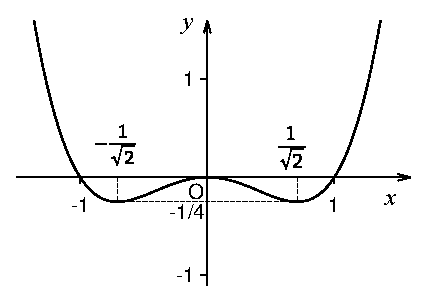
\includegraphics[width=7cm]{xxxx_xx.eps}
    \caption{$y=x^4-x^2$のグラフ(実線)。\label{fig:xxxx_xx}}
\end{figure}

\begin{exmpl} $y=x^4-x^2$のグラフを描いてみよう。まずこれは偶関数である。
また, $x$軸との共有点($y=0$)は, $x=0, \pm 1$である。

次に極大と極小を求める。$f'(x)=4x^3-2x$だから, $x=0, \pm 1/\sqrt{2}$で
$f'(x)=0$となる。それぞれ極大・極小のどちらだろう?

$x=-1/\sqrt{2}$については, それより少し小さな$x$では$f'(x)<0$ (つまり$f(x)$は減少傾向), それより
少し大きな$x$では$f'(x)>0$ (つまり$f(x)$は増加傾向)となるから, そこでは
極小値$f(-1/\sqrt{2})=-1/4$をとる。$x=1/\sqrt{2}$についても同様である。

一方, $x=0$については, それより少し小さな$x$では$f'(x)>0$ (つまり$f(x)$は増加傾向), 
それより少し大きな$x$では$f'(x)<0$ (つまり$f(x)$は減少傾向)となるから, そこでは
極大値$f(0)=0$をとる。

$x\rightarrow\infty$で$f(x)\rightarrow\infty$であることを併せて
考えると, 図\ref{fig:xxxx_xx}のようなグラフになる。(例おわり)\end{exmpl}


以上でわかったように, なめらかな関数のグラフが極大値や極小値をとる場所では, 
微分係数は0である。しかし, その逆は必ずしも成り立たないことに注意しよう。
つまり, 微分係数が0であっても, 極大にも極小にもならない, という場合が
存在するのだ。\mv

\begin{exmpl}
$y=x^3$は$x=0$での微分係数は0だが, P.\pageref{fig:xxx-x}の
図\ref{fig:xxx-x}の点線で示されるように, $y=x^3$の
グラフは, $x=0$で極大にも極小にもならない。
(例おわり)\end{exmpl}
\vv




\section{偶関数や奇関数の微分}

関数$f(x)$が偶関数であるとする。すなわち, $f(-x)=f(x)$が恒等的に成り立つ。
この両辺を$x$で微分すると, $-f'(-x)=f'(x)$となる(左辺は合成関数の微分!)。
すなわち, $f'(-x)=-f'(x)$が恒等的に成り立つ, すなわち$f'(x)$は奇関数
である。偶関数の導関数は奇関数なのだ!

\begin{comment}
その導関数を$f'(x)$とすると, \eref{eq:define_dif10}より, 
\begin{eqnarray}f'(x)=\frac{f(x+dx)-f(x)}{dx}\label{eq:diff_evenfunc0}\end{eqnarray}
である。この式で, 形式的に, $x$を$-x$に, $dx$を$-dx$に書き換えると
\begin{eqnarray}f'(-x)=\frac{f(-x-dx)-f(-x)}{-dx}\end{eqnarray}
となるが, $f(x)$は偶関数なので, 
\begin{eqnarray}f(-x)=f(x),\,\,\, f(-x-dx)=f(x+dx)\end{eqnarray}
なので, 
\begin{eqnarray}
f'(-x)&=&\frac{f(x+dx)-f(x)}{-dx}\\
      &=&-\frac{f(x+dx)-f(x)}{dx}=-f'(x)\end{eqnarray}
従って, $f'(x)$は奇関数である。

\begin{freqmiss}{\small\textgt{上の論証過程で, 「$x=-x$, $dx=-dx$とすると」
と書いてしまう} ... もし$x=-x$なら, 右辺を左辺に移項して$2x=0$, 従って$x=0$
となってしまう! 同様に, $dx=0$となってしまう! $x=-x$と書きたい気持ちは
わからなくもないですが, ひとつの等式の中に現れる以上は, 左辺の$x$と右辺の$x$は
同じ数として扱わざるを得ません。そもそも, \eref{eq:diff_evenfunc0}
はどんな$x$にも成り立つから, 「$x$のところを$-x$と書きなおしてもよかろう」
と考えるのだけど, それを$x=-x$と書いてしまうのは乱暴です。}\end{freqmiss}

\begin{freqmiss}{\small\textgt{上の論証過程で, 「$dx$を$-dx$に」という
部分を省略してしまう} ... そうしたい気持ちはわからなくもないですが, $x$と$dx$は
別の量。$x$を$-x$に置き換えたからといって, $dx$も自動的に$-dx$に
置き換わるものではないのです。}\end{freqmiss}
\hv
\end{comment}

%------------
\begin{q}\label{q:diff_odd} 奇関数の導関数は偶関数であることを示せ。\end{q}
\mv

%------------
\begin{q}\label{q:diff_oddeven} $n$を0以外の任意の整数とする。
以下の関数について, 偶関数の導関数が奇関数になり, 
奇関数の導関数が偶関数になることを実際に確認せよ。なお, 
単に「確認した」というだけではレポートにはなりません!
\begin{edaenumerate}
\item $f(x)=x^{2n}$
\item $f(x)=x^{2n+1}$
\item \begin{eqnarray*}f(x)=\frac{1}{1+x^2}\end{eqnarray*}
\item \begin{eqnarray*}f(x)=\frac{x}{1+x^2}\end{eqnarray*}
\end{edaenumerate}\end{q}
ヒント: (3), (4)は問\ref{q:diff_func5}に出てきた。\mv

%\begin{q}\label{q:differential_English} 以下の言葉を英訳せよ:
%\begin{edaenumerate}<3>
%\item 微分する
%\item 導関数
%\item 変位
%\item 距離
%\item 速さ
%\item 速度
%\item 加速度
%\end{edaenumerate}
%\end{q}\mv

%\section*{一問一答}
%\begin{itemize}\item 無限大×無限小は?\end{itemize}
% 場合によります。$x$が無限大になるときには, $x\times(1/x)$や$x^2\times(1/x)$, 
%$x\times(1/x^2)$などは, いずれも「無限大×無限小」になりますが, 最初のは1になり, 
%2番めのは無限大になり, 最後のは0になります。

%\section*{一問一答}

%\begin{itemize}
%\item はじめて微分係数を考えた人はすごいと思った。
%\end{itemize}
% ニュートンとかライプニッツだと言われていますが, 実はそれより前に, 
%江戸時代の日本の数学者である関孝和も微分に近い概念を発見したそうです。関孝和には多くの
%素晴らしい業績があります。

%\begin{itemize}
%\item 微分の$f'(x)$の「'」は誰が決めたんですか?
%\end{itemize}
% ラグランジュです。$df/dx$という書き方はライプニッツが決めました。君が習う
%数学は, 物理学とともに18世紀〜19世紀頃に大きく発展した内容です。そこには何人かの
%スーパースターがいます。ラグランジュ, ライプニッツ, ニュートン, ガウス, オイラー, 
%コーシー, ラプラス, ダランベール等という名前は, これから何回も目にするでしょう。
%ちなみにラグランジュはマリー・アントワネットの数学教師だったそうです。


\begin{faq}\small{\textgt{数IIIをやっていないのでテストができません。}
... もう高校時代は終わったのだから「XXXをやって
いないから」というのはやめましょう。やっていなければ, 今, やればいいのです。
高校で数IIIをやった人も, それなりの苦労や努力をしたのです。}\end{faq}
\hv



\section*{演習問題}


\begin{exq} 
\begin{enumerate}
\item $y=1/x^n$と置き, その両辺を$x^n$倍し, その両辺を$x$で微分する, 
という発想で, \eref{eq:xpowminusn1}を導け。
\item $y=x^{1/n}$と置き, その両辺を$n$乗し, その両辺を$x$で微分する, 
という発想で, \eref{eq:xpowfrc}を導け。
\end{enumerate}
\end{exq}

\begin{exq} 逆関数の微分の公式 (\eref{eq:diff_form5})を, グラフの「接線の傾き」
という観点で示せ。ヒント: 逆関数のグラフは, もとの関数を, 
直線$y=x$に関して対称移動したもの。\end{exq}

\begin{exq}\label{q:diff_Legendre} $n$を0以上の整数とするとき, 以下の式で定義される
関数$P_n(x)$をルジャンドル関数\index{るじゃんどるかんすう@ルジャンドル関数}という
\footnote{この関数は, 実は原子の電子軌道(K殻とかL殻とか)
と密接な関係がある。}
\begin{eqnarray}
P_n(x) :=\frac{1}{2^n n!}\,\frac{d^n}{dx^n}(x^2-1)^n
\end{eqnarray}
\begin{enumerate}
\item $n=0, 1, 2, 3, 4$のそれぞれについて, $P_n(x)$を求めよ。
%\item $n=0, 1, 2, 3, 4$のそれぞれについて, $P_n(1)=1$であることを示せ。
\item $n$が偶数のときは$P_n(x)$は偶関数であることを示せ。
\item $n$が奇数のときは$P_n(x)$は奇関数であることを示せ。
\end{enumerate}
\end{exq}
\vv

\section*{問題の解答}

%\noindent{\textbf{答}}\ref{q:diff_def00} 略 (がんばれ!)\mv

%
\noindent{\textbf{答}}\ref{q:diff_def0}  無限小$dx$に対して, 
$g(a+dx) = g(a)+g'(a)dx$
と書けるとき, 右辺の$dx$の係数$g'(a)$のこと。もしくは, 
\begin{eqnarray*}g'(a)=\lim_{\Delta x \to 0} \frac{g(a+\Delta x)-g(a)}{\Delta x}\end{eqnarray*}
のこと(どちらでも可)。{\small 注: この問題で, あなたは
$g$を$f$と書いたり$a$を$x_0$と書いたりしなかっただろうか? 
本文に出てきた$f(x)$や$x_0$という記号は, 説明のための
便宜的なものであり, この問題のように, 設定に応じて変わるものである。}
\mv

%
\noindent{\textbf{答}}\ref{q:diff_const} 
\begin{eqnarray*}
f(x+dx)&=&p(x+dx) + q=px+q+p\,dx\\
       &=&f(x)+p\,dx
\end{eqnarray*}
$dx$の係数に着目して, $f'(x)=p$。
特に, $f(x)$が定数関数の場合は$p=0$だから, 
$f'(x)$は恒等的に0。\qed
\mv

% 表計算ソフトで, 関数$f(x)=x^2$を, $-2 \le x \le 2$の範囲で数値微分し, 
%\noindent{\textbf{答}}\ref{q:comp_diff0} 略。\mv

% 以下の関数を微分せよ:
\noindent{\textbf{答}}\ref{q:diff_func0}
\begin{edaenumerate}
\item $f'(x)=2x+1$
\item $f'(x)=8x+5$
\item $f'(x)=6x+3$
\item $f'(x)=-5/x^2$
\item $f'(x)=1+1/x^2$
\end{edaenumerate}

% 以下の関数:\begin{eqnarray}f(x)=(x^2+x+1)(x^2-x-2)\end{eqnarray}について, 
\noindent{\textbf{答}}\ref{q:diff_func1}
\begin{eqnarray*}
(1)\quad f'(x)&=&(x^2+x+1)'(x^2-x-2)\\
     &+&(x^2+x+1)(x^2-x-2)'\\
     &=&(2x+1)(x^2-x-2)\\
     &+&(x^2+x+1)(2x-1)\\
     &=&4x^3-4x-3\\
(2)\quad f(x)&=&x^4-2x^2-3x-2\\
f'(x)&=&4x^3-4x-3
\end{eqnarray*}

% 以下の関数を, 合成関数の微分の公式を使って微分せよ:
\noindent{\textbf{答}}\ref{q:diff_func2}
\begin{enumerate}
\item ($g(x)=x^3$, $f(x)=3x^2+2$とみなせばよい。)
\begin{eqnarray*}
F'(x)&=&3(3x^2+2)^2(3x^2+2)'\\
     &=&3(3x^2+2)^2(6x)=18x(3x^2+2)^2\end{eqnarray*}
\item ($g(x)=x^3$, $f(x)=x^2+x+1$とみなせばよい。)
\begin{eqnarray*}
F'(x)&=&3(x^2+x+1)^2(x^2+x+1)'\\
     &=&3(x^2+x+1)^2(2x+1)
\end{eqnarray*}
\item ($g(x)=x^2, f(x)=x^5+x^4+x^3+x^2+x+1$とみなせばよい。)
\begin{eqnarray*}
F'(x)=2&(x^5+x^4+x^3+x^2+x+1)\\
       &\,\,\times(x^5+x^4+x^3+x^2+x+1)'\\
     =2&(x^5+x^4+x^3+x^2+x+1)\\
       &\,\,\times(5x^4+4x^3+3x^2+2x+1)
\end{eqnarray*}
\item ($g(x)=x^2$, $f(x)=1+1/x$とみなせばよい。)
\begin{eqnarray*}
F'(x)&=&2\Bigl(1+\frac{1}{x}\Bigr)\Bigl(1+\frac{1}{x}\Bigr)'\\
     &=&-2\Bigl(1+\frac{1}{x}\Bigr)\frac{1}{x^2}=-2\Bigl(\frac{1}{x^2}+\frac{1}{x^3}\Bigr)
\end{eqnarray*}
\end{enumerate}

% 関数$g(x)$の逆数であらわされる関数$1/u(x)$の導関数は, 以下で与えられることを示せ:
\noindent{\textbf{答}}\ref{q:diff_func3} 関数$1/u(x)$は, 関数$1/x$と関数$u(x)$の合成関数である。$(1/x)'=-1/x^2$だから, 
\begin{equation*}
\Bigl(\frac{1}{u}\Bigr)'=\Bigl(-\frac{1}{u^2}\Bigr)u'=-\frac{u'}{u^2}
\end{equation*}

% 関数$f(x)$と$u(x)$の比で作られる関数$f(x)/u(x)$の導関数は, 以下で与えられることを示せ:
\noindent{\textbf{答}}\ref{q:diff_func4} 関数$v(x)/u(x)$は, 関数$v(x)$と関数$1/u(x)$の積である。
\begin{eqnarray*}
\Bigl(v\times\frac{1}{u}\Bigr)'&=&v'\Bigl(\frac{1}{u}\Bigr)+v\Bigl(\frac{1}{u}\Bigr)'\\
&=&v'\Bigl(\frac{1}{u}\Bigr)+v\Bigl(-\frac{u'}{u^2}\Bigr)=\frac{v'u-vu'}{u^2}
\end{eqnarray*}

% 以下の関数を微分せよ:
\noindent{\textbf{答}}\ref{q:diff_func5}
\begin{edaenumerate}
\item \begin{eqnarray*}-\frac{2x}{(1+x^2)^2}\end{eqnarray*}
\item \begin{eqnarray*}\frac{1-x^2}{(1+x^2)^2}\end{eqnarray*}
\end{edaenumerate}

% べき関数の微分の公式を使って, 以下の関数を微分せよ。
\noindent{\textbf{答}}\ref{q:diff_pow} 
\begin{edaenumerate}
\item \begin{eqnarray*}-\frac{1}{x^2}\end{eqnarray*}
\item \begin{eqnarray*}-\frac{1}{2x^{3/2}}=-\frac{1}{2}x^{-3/2}\end{eqnarray*}
\item \begin{eqnarray*}\frac{2}{3}x^{-1/3}\end{eqnarray*}
\item \begin{eqnarray*}-5x^{-6}\end{eqnarray*}
\end{edaenumerate}

% 微分の公式1〜5を証明せよ。
%\noindent{\textbf{答}}\ref{q:diff_theories1_5} 略(本文参照)。\hv

% 以上の微分の公式を駆使して, 以下の関数を微分せよ:
\noindent{\textbf{答}}\ref{q:diff_func8}
\begin{enumerate}
\item ヒント: $g(x)=\sqrt{x}$, $f(x)=2x+3$として公式4を使う。$g'(x)=1/(2\sqrt{x})$だから, 
\begin{eqnarray*}\text{(与式)}'=\frac{f'(x)}{2\sqrt{f(x)}}=\frac{(2x+3)'}{2\sqrt{2x+3}}=\frac{2}{2\sqrt{2x+3}}\\
=\frac{1}{\sqrt{2x+3}}\end{eqnarray*}
\item ヒント: $g(x)=\sqrt{x}$, $f(x)=1-x^2$として公式4を使う。$g'(x)=1/(2\sqrt{x})$だから, 
\begin{eqnarray*}\text{(与式)}'=\frac{f'(x)}{2\sqrt{f(x)}}=\frac{(1-x^2)'}{2\sqrt{1-x^2}}=\frac{-2x}{2\sqrt{1-x^2}}\\
=-\frac{x}{\sqrt{1-x^2}}\end{eqnarray*}
\item ヒント: まず$x^2$と$\sqrt{1+x^2}$の積と考えて公式3を使う。その上で例\ref{exmpl:diff_sqrtx2p1}を使う。
\begin{eqnarray*}\text{(与式)}'=(x^2)'\sqrt{1+x^2}+x^2(\sqrt{1+x^2})'\\
=2x\sqrt{1+x^2}+\frac{x^3}{\sqrt{1+x^2}}\end{eqnarray*}
\item ヒント: $g(x)=x^{-1/2}$, $f(x)=1+x^2$として公式4を使う。
\begin{eqnarray*}&&\text{(与式)}'=\frac{-1}{2}(f(x))^{-3/2}f'(x)\\
&&=\frac{-1}{2}(1+x^2)^{-3/2}(2x)=-\frac{x}{(1+x^2)^{3/2}}\end{eqnarray*}
\item ヒント: $g(x)=1/x$, $f(x)=1+\sqrt{x}$として公式4を使う。
\begin{eqnarray*}&&\text{(与式)}'=-\frac{(1+\sqrt{x})'}{(1+\sqrt{x})^2}\\
&&=-\frac{\frac{1}{2\sqrt{x}}}{(1+\sqrt{x})^2}=-\frac{1}{2\sqrt{x}(1+\sqrt{x})^2}\end{eqnarray*}
\item ヒント: $g(x)=\sqrt{x}$, $f(x)=1+1/x$として公式4を使う。
\begin{eqnarray*}\text{(与式)}'
=\frac{1}{2\sqrt{1+\frac{1}{x}}}\Bigl(1+\frac{1}{x}\Bigr)'=\frac{-1}{2x^2\sqrt{1+\frac{1}{x}}}\end{eqnarray*}
\item ヒント: $x-1$と$1/(x+1)$の積と考えて公式3を使う。
\begin{eqnarray*}\text{(与式)}'=(x-1)'\frac{1}{x+1}+(x-1)\Bigl(\frac{1}{x+1}\Bigr)'\\
=\frac{1}{x+1}-(x-1)\frac{1}{(x+1)^2}=\frac{2}{(x+1)^2}\end{eqnarray*}
別解: 与式=$1-2/(x+1)$と変形してから微分しても, 同じ結果になる。
\item ヒント: $g(x)=1/x$, $f(x)=1+1/x$として公式4を使ってもよいのだが, 
与式を変形してから微分するほうが簡単。与式の分母分子に$x$をかけて, 
\begin{eqnarray*}\text{(与式)}=\frac{x}{x+1}=1-\frac{1}{x+1}\end{eqnarray*}
従って, 
\begin{eqnarray*}\text{(与式)}'=\Bigl(1-\frac{1}{x+1}\Bigr)'=\frac{1}{(x+1)^2}\end{eqnarray*}
\end{enumerate}
\hv


% 解答: 線型近似
\noindent{\textbf{答}}\ref{q:univ_lin_approx0}  \
$f(x)=(1+x)^a$と置くと, $f(0)=1$。また, $f'(x)=a(1+x)^{a-1}$なので, 
従って$f'(0)=a$。これを\eref{eq:linear_approx00}に入れると, 与式を得る。\mv

\noindent{\textbf{答}}\ref{q:univ_lin_approx2}  \
\begin{enumerate}
\item \eref{eq:linear_approx02}で$a=-1$とすれば, $1/(1+x)\fallingdotseq1-x$
\item 前小問の$x$を$-x$に置き換えて, $1/(1-x)\fallingdotseq1+x$
\item \eref{eq:linear_approx02}で$a=-1/2$とすれば, \\$1/\sqrt{1+x}\fallingdotseq1-x/2$
\end{enumerate}
\mv

\noindent{\textbf{答}}\ref{q:univ_lin_approx4} 
\begin{enumerate}
\item $(0.99)^{10}=(1-0.01)^{10} \fallingdotseq 1-10 \times 0.01=0.9$
\item 3乗して10に近い簡単な数は何かな?と考えると, 2が思いつく。$2^3=8$であることに
注目し, 
\begin{eqnarray*}
10^{1/3}&=&(8+2)^{1/3}=\Bigl\{8\Bigl(1+\frac{2}{8}\Bigr)\Bigr\}^{1/3}\\
&=&8^{1/3}\Bigl(1+\frac{2}{8}\Bigr)^{1/3}=2\Bigl(1+\frac{1}{4}\Bigr)^{1/3}\\
&\fallingdotseq&2\Bigl(1+\frac{1}{3\times4}\Bigr)=2+\frac{1}{6}=2.166\cdots
\end{eqnarray*}
\end{enumerate}
\mv

% 以下の関数について, $f'(x)$, $f''(x)$, $f^{(3)}(x)$をそれぞれ求めよ。
\noindent{\textbf{答}}\ref{q:diff_func9}
\begin{edaenumerate}
\item
\begin{eqnarray*}
&&f'(x)=5x^4+6x^2\\
&&f''(x)=20x^3+12x\\
&&f^{(3)}(x)=60x^2+12
\end{eqnarray*}
\item
\begin{eqnarray*}
&&f'(x)=\frac{1}{(1-x)^2}\\
&&f''(x)=\frac{2}{(1-x)^3}\\
&&f^{(3)}(x)=\frac{6}{(1-x)^4}
\end{eqnarray*}
\end{edaenumerate}

% $n$を0以上の整数とするとき, 以下の式で定義される
%\noindent{\textbf{答}}\ref{q:diff_Legendre}
%\begin{eqnarray*}
%P_0(x)&=&\frac{1}{2^00!}(x^2-1)^0=1\\
%P_1(x)&=&\frac{1}{2^11!}(x^2-1)'=\frac{2x}{2}=x\\
%P_2(x)&=&\frac{1}{2^22!}\{(x^2-1)^2\}''=\frac{(x^4-2x^2+1)''}{8}\\
%      &=&\frac{12x^2-4}{8}=\frac{3x^2-1}{2}\\
%P_3(x)&=&\frac{1}{2^33!}\{(x^2-1)^3\}'''=\frac{(x^6-3x^4+3x^2-1)'''}{48}\\
%      &=&\frac{120x^3-72x}{48}=\frac{5x^3-3x}{2}
%\end{eqnarray*}
%\hv

\noindent{\textbf{答}}\ref{q:diff_def} (1), (2), (3)は略。
本文をよく読めば簡単。(4) 「距離を」ではなく「位置を」と言わねばならない。距離を
時刻で微分したものは「速さ」である。(5) 間違っているとは言い切れないが, 
「時刻によって微分」と言わねば不正確である。\mv

% 点Pが, $x$軸上を運動している。時刻$t$のときPの位置が$x=t^2-3t+1$と書けるとき
\noindent{\textbf{答}}\ref{q:diff_velocac} (1) 位置を時刻で微分する: $(at^2+bt+c)'=2at+b$。
(2) 再度時刻で微分する: $(2at+b)'=2a$。\mv

\noindent{\textbf{答}}\ref{q:diff_velocac1} 
問\ref{q:diff_velocac}(2)で, $2a$が加速度なので, $a$は加速度の次元(SI単位ではm~s$^{-2}$)。
問\ref{q:diff_velocac}(1)で, $2at+b$が速度なので, $b$は速度の次元(SI単位ではm~s$^{-1}$)。
もともと$x=at^2+bt+c$だったので, $c$は$x$と同じ次元(長さ; SI単位ではm)。\mv

\noindent{\textbf{答}}\ref{q:diff_velocac2}(略解) 位置は503~m。速度は99~m~s$^{-1}$。
加速度は9.8~m~s$^{-2}$。\mv

\noindent{\textbf{答}}\ref{q:vect_throw} ${\bf r}(t)=(v_0t,\, -gt^2/2)=(x, y)$と置く。
(1) $x, y$から$t$を消去して, $y=-gx^2/(2v_0^2)$。これを$xy$平面にプロットすると, 
原点を頂点とする, 上に凸の放物線になる。 (2) ${\bf v}(t)={\bf r}'(t)=(v_0,\, -gt)$  
(3) ${\bf a}(t)={\bf v}'(t)=(0,\, -g)$。なお, この点の運動は, 水平方向に初速$v_0$で投げたボールの運動である。\mv


% 奇関数の導関数は偶関数であることを示せ。
\begin{comment}
\noindent{\textbf{答}}\ref{q:diff_odd} 
 関数$f(x)$が奇関数であるとする。その導関数を$f'(x)$とすると, 導関数の定義より, 
\begin{eqnarray}f'(x)=\frac{f(x+dx)-f(x)}{dx}\end{eqnarray}
である。この式で, 形式的に, $x$を$-x$に, $dx$を$-dx$に書き換えると
\begin{eqnarray}f'(-x)=\frac{f(-x-dx)-f(-x)}{-dx}\end{eqnarray}
となるが, 奇関数の定義より$f(-x)=-f(x)$, $f(-x-dx)=-f(x+dx)$なので, 
\begin{eqnarray}f'(-x)&=&\frac{-f(x+dx)+f(x)}{-dx}\nonumber\\
&=&\frac{f(x+dx)-f(x)}{dx}=f'(x)\end{eqnarray}
従って, $f'(x)$は偶関数である。\qed
\hv
\end{comment}

% 
\noindent{\textbf{答}}\ref{q:diff_oddeven} (1) $f(-x)=(-x)^{2n}=
(-1)^{2n}x^{2n}=x^{2n}=f(x)$。よって$f(x)$は偶関数。$f'(x)=2nx^{2n-1}$。
$f'(-x)=2n(-x)^{2n-1}=(-1)^{2n-1}2nx^{2n-1}=-2nx^{2n-1}=-f'(x)$。
よって$f'(x)$は奇関数。(2)以下略。

\begin{comment}
図\ref{fig:even_odd_function}参照。
\begin{figure}[h]
    \centering
    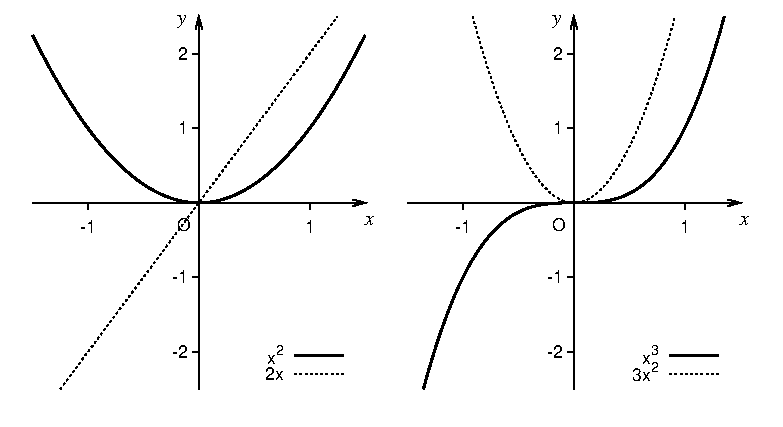
\includegraphics[width=8cm]{even_odd_function.eps}
    \caption{左:$y=x^2$(実線)と$y=2x$(破線)のグラフ。右:$y=x^3$(実線)と$y=3x^2$(破線)のグラフ。}\label{fig:even_odd_function}
\end{figure}
\end{comment}


%\include{05_differential_ans}
\chapter{指数・対数}\label{chapt_exp_log}
{\small 過去の受講生の言葉: 「最近ようやく定義を1つずつ確認する癖がつき, 理解しやすくなった。」}

%{\small 基礎がしっかりしていて, 子供のようなミスは決して犯さない。
%それが真剣さというものだ (イビチャ・オシム 元サッカー日本代表監督)。\\}

\section{指数関数}

$a$を正の定数とし, $a^x$という関数を考えよう。こういう関数を
\underline{指数関数}\index{しすうかんすう@指数関数}という。例えば$a=2$のときは, 
$2^x$であり, これは$x=0, 1, 2, 3, 4$のときは
それぞれ, 1, 2, 4, 8, 16, ...と, 急速に大きくなる。パソコンを使って
$y=2^x$をグラフに描くと, \fref{fig:y2powx}の実線のようになる。
\begin{figure}[h]
    \centering
    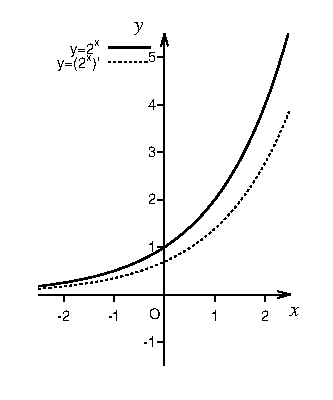
\includegraphics[width=6.0cm]{y2powx.eps}
    \caption{$y=2^x$と$y=(2^x)'$のグラフ}\label{fig:y2powx}
\end{figure}
ここで, $y=2^x$を数値微分した結果(つまり導関数)も点線で描いた。
これを見ると, $y=2^x$とその導関数はちょっと似ている。それは, 
$y=2^x$が急激な右肩上がりの曲線なので, 右に行くほど接線の
傾きも急速に大きくなる, 従って, 導関数(接線の傾きの値を
並べたもの)も右肩上がりになるのだ。

では, 同じようなことを$y=3^x$についてやってみたらどうだろう?
結果は, \fref{fig:y3powx}のようになる。
\begin{figure}[h]
    \centering
    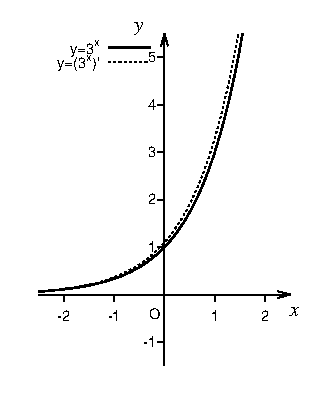
\includegraphics[width=6.0cm]{y3powx.eps}
    \caption{$y=3^x$と$y=(3^x)'$のグラフ}\label{fig:y3powx}
\end{figure}
やはり, $y=3^x$は急激に右肩上がりの曲線で, その導関数も似ている。
\fref{fig:y2powx}と\fref{fig:y3powx}を比べてみると, 
\fref{fig:y3powx}の方が, もとの関数と導関数はずっと近い。しかし, 
\fref{fig:y2powx}ではもとの関数よりも導関数の方が下にあったのが, 
\fref{fig:y3powx}ではやや上にある。ということは, $a$が3よりも若干
小さい数では, $y=a^x$とその導関数がぴったり一致するのではない
だろうか? 実はそうなのである。いろいろ試すと, $a$が$2.71828\cdots$
のときにそうなるのだ。これが, \pref{eq:NapierNum_value}
で出てきた\underline{ネイピア数}\index{ねいぴあすう@ネイピア数}$e$の正体である。すなわち, 
\begin{eqnarray}
(e^x)'=e^x\label{eq:exp_diff}
\end{eqnarray}
となるような数$e$をネイピア数と言うのだ。そして, $e^x$は, 
「微分しても変わらない指数関数」である。$e^x$のことを, \underline{エクスポーネンシャル} 
(exponential)\index{えくすぽーねんしゃる@エクスポーネンシャル} と呼ぶ。
なお, 第1章で述べたように, $e^x$を, $\exp x$\index{exp}と書くことも多い。
単なる書き方の約束だが, 意外に見落とす人がいるので, もういちど大きく書いておこう:

\begin{itembox}{約束}
\begin{eqnarray}\exp x :=e^x\end{eqnarray}
\end{itembox}

\begin{q}\label{q:exp_graph0} 表計算ソフトで, $y=2.718^x$のグラフと, 
$y=2.718^x$を数値微分したグラフを, 重ねて描いてプリントアウトせよ。$x$の
刻みは0.01くらいでよい。$x$の範囲は$-2$以上2以下としよう。\end{q}

実は, ネイピア数$e$は, 次式を満たす:
\footnote{$dx$を微小量とする。$e$が$(e^x)'=e^x$を満たすなら, 
微分の定義より, $e^{x+dx}=e^x+e^xdx$のはず。従って, 
$e^{x+dx}=e^x(1+dx)$。一方, 指数法則より, $e^{x+dx}=e^xe^{dx}$。
これらを比べて, $e^{dx}=1+dx$。両辺を$1/dx$乗して, $e=(1+dx)^{1/dx}$。
$dx$を$h$に置き換えたら\eref{eq:def_NapierNum0}になる。}
\begin{eqnarray}
e=\lim_{ h \to 0} ( 1 + h)^{1/h}\label{eq:def_NapierNum0}
\end{eqnarray}
あるいは, $1/h$を$n$と置き換えて, 
\begin{eqnarray}
e=\lim_{n \to \infty} \Bigl( 1 + \frac{1}{n} \Bigr)^n\label{eq:def_NapierNum}
\end{eqnarray}

\begin{q}\label{q:exp_evalue} \eref{eq:def_NapierNum}のlimの内側を, 
$n=2$, $n=10$, $n=100$, $n=1000$, $n=10000$の
各場合について, 関数電卓で計算せよ。
\end{q}

\begin{q}\label{q:def_NapierNum} \eref{eq:def_NapierNum0}, \eref{eq:def_NapierNum}
をそれぞれ5回書いて記憶せよ。\end{q}

\begin{freqmiss}{\small\textgt{\eref{eq:def_NapierNum}で, 
$n$を$\infty$ではなく0に近づける極限と勘違いして覚えてしまう} ... 
仮に$n$を0.01や0.001などとして\eref{eq:def_NapierNum}を電卓で計算して
ごらん。2.718$\cdots$ではなく1に近づいて行ってしまいます。}\end{freqmiss}

%\begin{faq}\small{\textgt{関数電卓って便利ですよね。買ったばかり
%のころ説明書を読んで,こんなにも多くの機能があるのかと感動しました。}
%... 数学を理解すれば関数電卓の威力は倍増します。}\end{faq}

実は, $e^x$は, 次のようにも表される\footnote{証明は以下の
通り: $1/n=x/N$と置こう($N$は適当な実数)。すると, $n=N/x$。
\eref{eq:def_NapierNum}のlimの内側にこれを入れると, 
$(1+x/N)^{N/x}$。$n\rightarrow\infty$のときはこれが
$e$に収束するので, この$x$乗, つまり$(1+x/N)^N$は$e^x$
に収束する。$n\rightarrow\infty$のとき$N\rightarrow\infty$
となるので, 
\begin{eqnarray*}
e^x=\lim_{N \to \infty} \Bigl( 1 + \frac{x}{N} \Bigr)^N
\end{eqnarray*}
となる。ここで改めて$N$を$n$と置き換えれば, \eref{eq:func_e_def}。}:
\begin{eqnarray}
e^x=\lim_{n \to \infty} \Bigl( 1 + \frac{x}{n} \Bigr)^n\label{eq:func_e_def}
\end{eqnarray}

\begin{q}\label{q:func_e_def} \eref{eq:func_e_def}のlimの内側を, 
$x=2$, $n=10000$について電卓で計算せよ。$e^2$も電卓で計算し, 
それらを比べよ。$x=-1$, $n=10000$についても同様の比較を行え。\end{q}

\eref{eq:func_e_def}は\eref{eq:def_NapierNum}を拡張した形の式になっている。
これを使うと, 以下のような問題が楽に扱える:\hv

\begin{exmpl} 貯金すると, お金に利子がつく。一年間の利率が$r$
の場合, $x$円のお金を銀行に預けると一年後には$rx$円の利子がついて, 
お金は$x+rx=(1+r)x$円になる。つまり, $(1+r)$倍になる。もう一年預けると, 
お金はさらに$(1+r)$倍になり, $(1+r)^2x$円になる。そういうふうに考えれば, 
$n$年後には, お金は$(1+r)^n$倍になることがわかる。\end{exmpl}

\begin{q}\label{q:func_exp_interest1} 以下の値を, 電卓を使って
小数第4位まで求めよ(5位を四捨五入せよ)。
\begin{enumerate}
\item 年間の利率が1\%, すなわち$r=0.01$のとき, 
預けたお金は100年間で何倍になるか?
\item 年間の利率が0.01\%, すなわち$r=0.0001$のとき, 
預けたお金は10000年間で何倍になるか? (それまで人類が
滅亡しなければ!)
\end{enumerate}
\end{q}

前問で, お金の倍率は, 2.718...という, $e$に近い値になっていった。なぜだろう?
$n$を年数と考えると, この問題では, $r=1/n$である。そして, ここで行った計算は, 
\eref{eq:def_NapierNum}のlim内をいろんな$n$の値について求めたのと
同じである。$n$が大きければ大きいほど\eref{eq:def_NapierNum}が使えるわけだ。

\begin{faq}{\small\textgt{問\ref{q:func_exp_interest1}(1)で, $1.01^{100}$を, 
\pref{eq:linear_approx02}でやった線型近似$(1+x)^a\fallingdotseq1+ax$
で計算したら, $1.01^{100}=(1+0.01)^{100}\fallingdotseq1+100\times0.01=1+1=2$
になってしまい, $2.7\cdots$にはなりません。何がおかしい?}
... 良いところに気づきました。その線型近似は, $a$が大きいと精度が悪いのです。}\end{faq}

\begin{q}\label{q:func_exp_interest3} 金利2\%で100年間, お金を借りたとき, 
お金は元金の何倍になるか? \eref{eq:func_e_def}を使って近似的に計算せよ。
\end{q}

\begin{q}\label{q:func_exp_disaster} ある地域で大災害をもたらす豪雨が, 
平均的に$n$年に1回の頻度でランダムに起きていることが過去の記録から
わかった($n$はある自然数)。豪雨は1年間に2回以上は起きないとする
\begin{enumerate}
\item その豪雨が, 今からの1年間に1回も発生しない確率を求めよ。
\item その豪雨が, 今からの2年間に1回も発生しない確率を求めよ。
\item その豪雨が, 今からの$n$年間に1回も発生しない確率を求めよ。
\item $n$が大きな値になると, 前小問の確率はどのような値に近づくか?
\item 平均的に1000年に1回起きる豪雨が, 1000年間に\textgt{1回以上}
発生する確率は? 有効数字4桁で。
\end{enumerate}
\end{q}

この問題は, 災害リスク等を評価・解析する上で, 最も基礎となる考え方でもある。

\begin{faq}{\small\textgt{ネイピア数$e$というやつの不思議さに
驚きました。いったいどんな人が考えたんでしょうか?} ... 
ベルヌーイとかオイラーらしいです。ネイピアというスコットランド人(対数を
発明した人)の名前がついていますが, ネイピアが発見したのではないそうです。
ちなみにネイピア数の神秘は, さらにもっと続きがあるのです。}\end{faq}

さて, 改めて$y=e^x$のグラフを見てみよう。どんな数も0乗は1だから, 
$e^0=1$である。従ってこのグラフは$(0, 1)$を通る。また, $x=1$のときは$y=e=2.718\cdots$だから, $(1, 2.718\cdots)$
を通る。$x$が1増えるたびに$y$は$2.718\cdots$倍になるので, $x$が大きくなるにつれて
このグラフは急速に上に伸びていくだろう。一方, $x=-1$のときは, 
$y=e^{-1}=1/e=1/2.718\cdots$となる。$x$が1小さくなるたびに$y$は$1/2.718\cdots$倍
になるので, $x$が負のほうに行くにつれて, グラフは急激に$x$軸に近づいて
来るだろう。そう考えると, $y=e^x$のグラフは図\ref{fig:y_expx}の実線のようになる。

図\ref{fig:y_expx}には, $y=e^{-x}$のグラフも示した。これは$y=e^x$のグラフを$y$軸に関して
対称移動したものだ(わからない人は\pref{sec:func_trans}の\ref{sec:func_trans}節を参照せよ)。\\
\begin{figure}[h]
    \centering
    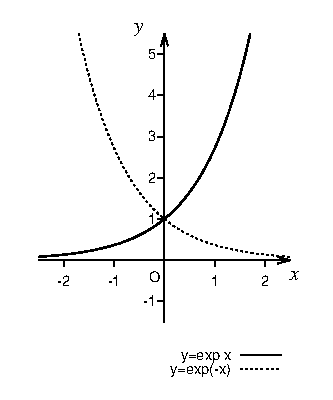
\includegraphics[width=6.0cm]{exp.eps}
    \caption{$y=\exp x$と$y=\exp(-x)$のグラフ}\label{fig:y_expx}
\end{figure}

\begin{q}\label{q:exp_graph1} 以下の関数のグラフを描け。
\begin{edaenumerate}
\item $y=1-e^{-x}$
\item $y=2(1-e^{-3x})$
\end{edaenumerate}\end{q}
\mv

さて, 指数関数を含む関数の微分を学ぼう。

\begin{exmpl} $f(x)=e^{-2x}$を微分してみよう。これを$e^y$と$y=-2x$の
合成関数と見れば(合成関数の微分を忘れた人は\pref{eq:diff_form4}へ!), 
\eref{eq:exp_diff}に注意して, 
\begin{eqnarray}f'(x)=e^{-2x}(-2x)'=-2e^{-2x}\end{eqnarray}
\end{exmpl}

\begin{exmpl} $f(x)=xe^{-2x}$を微分してみよう。まずこれを$x$と$e^{-2x}$の
積とみなして, 積の微分の公式(\pref{eq:diff_form3})より, 
\begin{eqnarray}f'(x)=e^{-2x}+x(e^{-2x})'\end{eqnarray}
右辺第二項の中の$(e^{-2x})'$は, 上の例より$-2e^{-2x}$となる。これらを組み合わせて, 
\begin{eqnarray}f'(x)=e^{-2x}-2xe^{-2x}=(1-2x)e^{-2x}\end{eqnarray}
\end{exmpl}

\begin{exmpl} $f(x)=e^{-a/x}$を微分してみよう($a$は定数)。これを$e^y$と$y=-a/x$の合成関数と見れば, 
\begin{eqnarray}f'(x)=e^{-a/x}\Bigl(-\frac{a}{x}\Bigr)'
=e^{-a/x}\Bigl(\frac{a}{x^2}\Bigr)=\frac{ae^{-a/x}}{x^2}\nonumber\\\end{eqnarray}
(例おわり)\end{exmpl}
\mv

\begin{q}\label{q:exp_diff0} 次の関数を微分せよ。
\begin{edaenumerate}
\item $f(x)=e^x$
\item $f(x)=e^{2x}$
\item $f(x)=\exp(-x^2)$
\item $f(x)=x \exp(-x^2)$
\end{edaenumerate}\end{q}
\mv


\section{対数}

第1章で学んだが, 正の実数$a, x$について($a\neq1$), 「$a$を何乗すると$x$になるか」
の指数を求める操作を, 
\begin{eqnarray}
\log_a x\label{eq:taisuu00_again}
\end{eqnarray}
とあらわす。これが対数の定義だった。ここで$a$にあたる数を\underline{底} \index{てい@底}, の$x$にあたる数を\underline{真数} \index{しんすう@真数}と呼ぶのだった。

この定義より, 
\begin{eqnarray}
\log_a x=y\label{eq:log1}
\end{eqnarray}
とは, 
\begin{eqnarray}
x=a^y\label{eq:log2}
\end{eqnarray}
と同じことである。\eref{eq:log1}を使って, \eref{eq:log2}右辺の$y$を$\log_a x$で置き換えられる。すると, 
\begin{eqnarray}
x=a^{\log_a x}\label{eq:log3}
\end{eqnarray}
となる。\eref{eq:log3}は対数の定義の言い換えにすぎないのだが, これが「わからない」
人が意外に多い。落ち着いて考えよう。$\log_a x$は, 「$a$を何乗すると
$x$になるか」である。\eref{eq:log3}の右辺は, その数で$a$を実際に「何乗かする」ことを意味
する。その結果が$x$になる(\eref{eq:log3}の左辺になる)のは当然である。\mv

注意: 対数を考える時は, 通常, 底と真数は正の実数とする。それらが負の状況は, 話が不必要にややこしくなるからである。例えば, 無理矢理に$\log_{-2}(-8)$を考えれば, それは3だろう($(-2)^3=-8$だから)。しかし, $\log_{2}(-8)$とか, $\log_{-2}8$は? と聞かれると困ってしまう。また, 通常, $1$は底として認めない。例えば$\log_{1}2$は? と聞かれると困ってしまうからだ。\mv

\begin{q}\label{q:exp_log0} $a$, $b$, $c$を正の実数として, 以下を示せ。
ただし$a \neq 1$とし, また, (8), (9)では$b \neq 1$とし, (10)では$c\neq 1$とする。
\begin{eqnarray}
&&\text{(1)}\,\,\,a^{\log_{a}b}=b\label{eq:apowlogab}\\
&&\text{(2)}\,\,\,\log_{a}a=1\\
&&\text{(3)}\,\,\,\log_{a}1=0\\
&&\text{(4)}\,\,\,\log_{a}b+\log_{a}c=\log_{a}bc\\
&&\text{(5)}\,\,\,\log_{a}\Bigl(\frac{1}{b}\Bigr)=-\log_{a}b\\
&&\text{(6)}\,\,\,\log_{a}\Bigl(\frac{b}{c}\Bigr)=\log_{a}b-\log_{a}c\label{eq:exp_log_formula6}\\
&&\text{(7)}\,\,\,\log_{a}b^c=c\log_{a}b\label{eq:log_power}\\
&&\text{(8)}\,\,\,\log_{a}b\times\log_{b}c=\log_{a}c\label{eq:logloglog}\\
&&\text{(9)}\,\,\,\log_{a}b=\frac{1}{\log_{b}a}\\
&&\text{(10)}\,\,\,\log_{a}b=\frac{\log_c b}{\log_c a}\label{eq:log_base_change}
\end{eqnarray}\end{q}
\hv

\eref{eq:log_base_change}は, \underline{底の変換公式} \index{ていのへんかんこうしき@底の変換公式}と呼ばれる。
これを使えば, どのような底の対数も, 特定の数を底とする対数の計算に変換できる。これは, 
電卓や計算機等による対数計算にしばしば有用である。\hv

\begin{exmpl} $\log_3 5$を関数電卓で求めてみよう。関数電卓の多くは, 
対数といえば常用対数や自然対数しか計算できないので, 底が3である$\log_3 5$は
直接は計算できない(ことが多い)。そこで, 底の変換公式を使って, 
$\log_3 5=\frac{\ln 5}{\ln 3}$としてやる。$\ln 5=1.609\cdots$や$\ln 3=1.098\cdots$
は関数電卓で計算できる。従って, 
\begin{eqnarray}
\log_3 5=\frac{\ln 5}{\ln 3}=\frac{1.609\cdots}{1.098\cdots}=1.464\cdots
\end{eqnarray}
と求まる。これを常用対数でやっても同じ結果になる: 
\begin{eqnarray}
\log_3 5=\frac{\log_{10} 5}{\log_{10} 3}=\frac{0.698\cdots}{0.477\cdots}=1.464\cdots
\end{eqnarray}
\end{exmpl}
\mv

\begin{q}\label{q:exp_logvalue} 以下を関数電卓で有効数字4桁で求めよ。
\begin{edaenumerate}
\item $\log_2 7$
\item $\log_{0.3} 5$
\end{edaenumerate}
\end{q}
\mv

\begin{q}\label{q:exp_log_ln} $x$を任意の正の実数とする。次式を示せ:
\begin{eqnarray}
&&\log_{10} x=(\log_{10} e)\times(\ln x)\fallingdotseq0.4343\ln x\label{eq:log2ln}\\
&&\ln x=(\ln 10)\times(\log_{10} x)\fallingdotseq2.3026\log_{10} x\label{eq:ln2log}
\end{eqnarray}\end{q}
\mv

世の中では, 対数といえば, 常用対数と自然対数がよく使われるので, 常用対数を
自然対数で表したり, その逆をしたり, というために, \eref{eq:logloglog}や
\eref{eq:log_base_change}がよく使われる。特に, ここで出てきた
\begin{eqnarray}
&&\log_{10} e\fallingdotseq0.4343\label{eq:log10e}\\
&&\ln 10\fallingdotseq2.3026\label{eq:ln10}
\end{eqnarray}
という2つの定数はよく現れる。

\begin{q}\label{q:log10e_ln10} 
\begin{enumerate}
\item \eref{eq:log10e}と\eref{eq:ln10}をそれぞれ5回書いて記憶せよ。
\item \eref{eq:log10e}と\eref{eq:ln10}の積が1になることを関数電卓を用いて確認せよ
\item それを数学的に証明せよ。
\end{enumerate}
\end{q}
\mv

ところで, $f(x)=e^x$と, $g(x)=\ln x$は, 互いに逆関数である。これは対数の定義から
明らかである。実際, 
\begin{eqnarray*}g(f(x))=\ln e^x=\log_e e^x=x\log_e e=x\end{eqnarray*}
となるし, 
\begin{eqnarray*}f(g(x))=\exp(\ln x)=e^{\log_e x}=x\end{eqnarray*}
となる(\eref{eq:apowlogab}より)。これはP.\pageref{eq:generaleq}の\eref{eq:generaleq}と整合的である。
図\ref{exp_log.eps}で明らかなように, $y=e^x$と$y=\ln x$のグラフは直線$y=x$
に関して互いに対称である(逆関数の性質。\pref{fig:func_revfunc}参照)。

\begin{figure}[h]
    \centering
    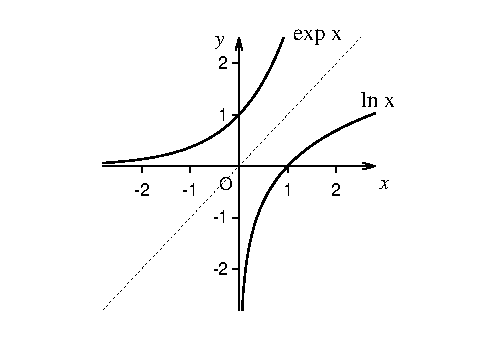
\includegraphics[width=7cm]{exp_log.eps}
    \caption{$y=e^x$と$y=\ln x$のグラフ。点線は, $y=x$のグラフ。}\label{exp_log.eps}
\end{figure}

ここで, $y=\ln x$のグラフは$0<x$の範囲でしか描かれていないことに注意。
つまり, $\ln x$という関数は, $x\le 0$では定義されない(考えることができない)
のだ。これは直感的にも明らかで, 例えば$\ln (-5)$は何か? などと言われても, 
$e=2.718\cdots$は, 何乗しようが必ず正の値であって, $-5$のような負の値は, とりようがない。

\begin{q}\label{q:exp_loggraph} 以下の関数のグラフを重ねて描け.
\begin{edaenumerate}<3>
\item $y=\log_{2}x$
\item $y=\ln x$
\item $y=\ln (1+x)$
\end{edaenumerate}\end{q}
\mv

次に, 対数関数の微分を考えよう。$f(x)=e^x$と$g(x)=\ln x$は互いに逆関数
であり, かつ, $f'(x)=f(x)$なので, 逆関数の微分(微分の公式5; \pref{eq:diff_form5})
により,
\begin{eqnarray}
(\ln x)'=g'(x)=\frac{1}{f'(g(x))}=\frac{1}{f(g(x))}=\frac{1}{x}
\label{eq:logdif}
\end{eqnarray}
である(ただし$0<x$とする)。つまり, \textgt{$\ln x$の微分は$1/x$になる}。このことは記憶せよ。
\mv

\begin{q}\label{q:exp_logdif_num} パソコンの表計算ソフトを使って, 
$\ln x$を数値微分せよ($0<x$とする)。その結果を, もとの関数($\ln x$)と, 解析的な
微分結果($1/x$)とともに, 重ねてグラフに描け。ヒント: $x=0$や$x<0$の
値では$\ln x$の計算がエラーになるので, 微妙に0より大きい$x$から始めよう。
結果は\fref{fig:difflnx}のようになるはず。
\end{q}
\begin{figure}[h]
    \centering
    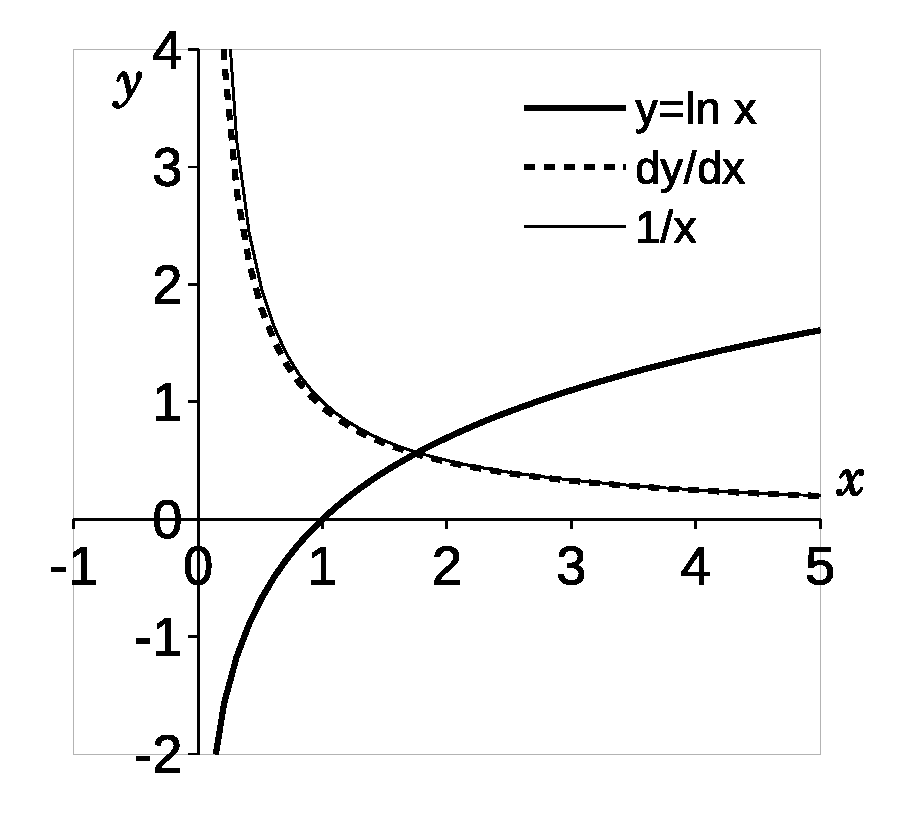
\includegraphics[width=6.5cm]{difflnx.eps}
    \caption{$y=\ln x$ (太い実線)とその数値微分(点線)のグラフ。
細い実線は$y=1/x$。$x$は0.05くらいから始めて, 刻みは0.1くらいにするときれいに描ける。}\label{fig:difflnx}
\end{figure}
\mv

\begin{q}\label{q:exp_logdif0} 以下の関数をそれぞれ微分せよ:
\begin{enumerate}
\item $\ln (x+1)$ ただし$-1<x$とする。
\item $\ln 2x$ ただし$0<x$とする。
\item $\ln |x|$ ただし$x\neq 0$とする。
\item $\ln (x-1)$ ただし$x<1$とする。
\item $\ln (1-x)$ ただし$x<1$とする。
\item $\ln |1-x|$ ただし$x\neq 1$とする。
\item \begin{eqnarray*}\ln \Bigl|\frac{x-1}{x+1}\Bigr|\quad\text{ただし}x\neq-1\text{かつ}x\neq 1\text{とする。}\end{eqnarray*}
\item $\log_{10} x$ ただし$0<x$とする。
\end{enumerate}
{\small
ヒント: (3)は$x<0$と$0<x$で場合分け。(6)は, $x<1$と$1<x$で場合分け。(7)は, いきなり合成関数の微分公式で処理するよりも, \eref{eq:exp_log_formula6}を使って変形すると楽。\\
注: これらの問題は, 「なんかややこしくてうざいな」と思うかもしれないが, 後で「積分」を学ぶときに重要な意味を持つ。また, (7)は, 生物の個体群変動を解析する理論で出てくる。}
\end{q}

\begin{faq}\small{\textgt{この問の(3)で, $\ln |x|$を微分すると$1/x$になってしまい, 絶対値が消えてしまいました。不思議です。} ... 場合分けしたのに, 結果は一緒って奇妙ですよね。図\ref{fig:difflnx}を使って考えてみましょう。$\ln |x|$のグラフは, この図を$y$軸でひっくり返して, 左右対称にしたものです。$y$軸の左側($x<0$)では, 左から$x=0$に近づくにつれて, $\ln |x|$は「奈落の底」に落ちていきます。つまり, 傾き(つまり$(\ln x)'$)はマイナス。といっても, $x=0$のはるか左では, 傾きはきつくないので, $(\ln x)'$はほぼ0。しかし, $x=0$に近づけば近づくほど傾きは急になるので, $(\ln x)'$の値はどんどん小さくなる(負の大きい値になる)。それはちょうど, $1/x$のグラフの, $x<0$での挙動によく似ている(というか一緒)です。}\end{faq}
\mv




\section{対数微分}

関数$f(x)=a^x$を微分してみよう(ただし$a$は1以外の正の定数とする)。このままではこの関数は微分できそうにない。そこで, まず, $f(x)=a^x$の両辺の
対数をとると, 
\begin{eqnarray}\ln f(x)=x\ln a\end{eqnarray}
ここで両辺を微分する。左辺の微分は, 合成関数の微分の公式から, 
\begin{eqnarray}\{\ln f(x)\}'=\frac{f'(x)}{f(x)}\end{eqnarray}
右辺の微分は, $\ln a$である。従って, 
\begin{eqnarray}\frac{f'(x)}{f(x)}=\ln a\end{eqnarray}
従って, 
\begin{eqnarray}f'(x)=(\ln a)f(x)=(\ln a)\,a^x\label{eq_diff_ax}\end{eqnarray}
となる。このように, 両辺の対数をとってから微分
するテクニックを\underline{対数微分} \index{たいすうびぶん@対数微分}という。\hv

\begin{q}\label{q:exp_diffxpowx} 対数微分を使って, 次式を示せ:
\begin{eqnarray}\frac{d}{dx}x^x=(1+\ln x)\,x^x\label{eq_diff_xx}\end{eqnarray}
ヒント: $f(x)=x^x$と置き, 両辺の$\ln$をとって, それらを$x$で微分。$x\ln x$の微分は
積の微分の公式を使う。
\end{q}

ちなみに, 問\ref{q:exp_diffxpowx}で考えた関数$x^x$のグラフは, 図\ref{fig:x_pow_x}
のようになる。これを見ると, \eref{eq_diff_xx}が0になるとき, つまり$x=1/e$で
最小値をとることがわかる。
\begin{figure}[h]
    \centering
    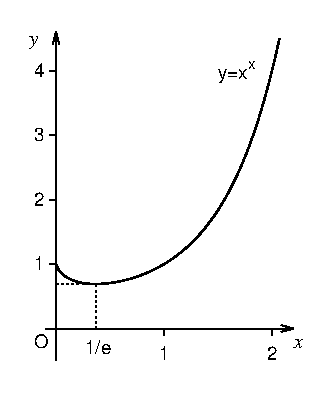
\includegraphics[width=4.5cm]{x_pow_x.eps}
    \caption{$y=x^x$のグラフ。}\label{fig:x_pow_x}
\end{figure}

\begin{freqmiss}{\small\textgt{$x^x$の微分を, 「$(x^{\alpha})'=\alpha x^{\alpha-1}$」という
公式(P.\pageref{eq:diff_form6}の\eref{eq:diff_form6})に「当てはめ」て, $(x^{x})'=x x^{x-1}=x^x$
としてしまう} ... $(x^{\alpha})'=\alpha x^{\alpha-1}$は, $\alpha$が定数の
ときにしか成り立ちません。この間違いでは, 指数部分の$x$を$\alpha$に見立てて
しまっていますが, $x$は定数ではないので, このような適用は許されません。
それに, $x=1/e$でこのグラフの傾きは0になっているので, そこでの微分係数は0
のはず。でも, $x^x$に$x=1/e$を入れたら, $(1/e)^{1/e}=0.692\cdots$で, 0に
なりません。だから, 少なくとも$x=1/e$では$(x^x)'=x^x$は成り立ちません。}\end{freqmiss}
\mv





\section{ガウス関数}\index{がうすかんすう@ガウス関数}
$a$を正の定数として, 
\begin{eqnarray}
f(x)=\exp(-ax^2)\label{eq:Gauss_func}
\end{eqnarray}
という形の関数を\underline{ガウス関数} (Gauss function)という。ガウス関数は, 統計学をはじめ, 様々な分野で
重要な関数なので, ここでいくつか性質を調べておこう。\mv

\begin{q}\label{q:exp_Gauss} ガウス関数に関して, 以下のことを示せ:
\begin{enumerate}
\item 偶関数である。
\item 常に0より大きい。
\item $f'(0)=0$である(だから$x=0$での接線は水平)。
\item $x$が大きくなると, 0に近づいていく。
\item $x=0$で最大値をとる。
\end{enumerate}\end{q}\mv

これらから, ガウス関数のグラフは, $x=0$を頂点とする, 左右対称の山形のグラフになることが
想像できる。\mv

\begin{q}\label{q:exp_Gauss_graph} 以上のことから, 
\begin{enumerate}
\item $a=1$のときのガウス関数のグラフを描け。
\item $a$が1より大きくなるとグラフはどう変わるか? 
\end{enumerate}\end{q}

\begin{figure}[h]
    \centering
    \includegraphics[width=7cm]{Gauss_fnc.eps}
    \caption{ガウス関数$y=\exp(-x^2)$のグラフ。常に$y>0$なので, 
本当は$x$軸と重なることは無いのだが, $x$がある程度大きくなると, 
非常に速く$x$軸に接近するので, $|x|$が3や4くらいになったら
$x$軸にぴったり重ねて描いてもかまわない(むしろその方が実情に近い)。
\label{fig:Gauss_func}}
\end{figure}

\begin{freqmiss}{\small\textgt{$y=\exp(-x^2)$のグラフを, $y=e^{-x}$のような左右非対称
なグラフを描いたり, 最大値のところで尖ったグラフを描いてしまう。} ... 偶関数のグラフは左右対称でしょ?}\end{freqmiss}
\mv


\section{対数グラフ}\index{たいすうぐらふ@対数グラフ}

実験データの解析等で, 軸が対数で目盛られたグラフをよく使う。図\ref{fig:log_graph}は, 
横軸は普通の目盛だが縦軸が対数目盛になったグラフである。このように片方の軸が
対数目盛のグラフを\underline{片対数グラフ} \index{かたたいすうぐらふ@片対数グラフ}という。
対数軸には, 以下のような特徴がある:
\begin{itemize}
\item "0"が存在しない。下に行くほど0に近づくが, 決して0をグラフ上で表現することはできない。
\item 太い目盛りをひとつ移動すれば値が10倍になる。
\item 細い目盛りをひとつ移動すれば最上位の桁の値がひとつ増える。
\end{itemize}

\begin{figure}[h]
    \centering
    \includegraphics[width=8cm]{log_paper.eps}
    \caption{片対数グラフの例。左の軸に振られている目盛りは, 対数にする前の値の目盛り(だから変な間隔になっている; グラフ上に点を打つときは便利)。右の軸に振られている目盛りは, 対数にした後の値の目盛り。直線の傾きは右側の目盛りで求める。なお, 
世の中の多くの対数グラフでは, 左のような軸か, 右のような軸のどちらか片方だけが, 左側に書かれている。\label{fig:log_graph}}
\end{figure}

例えば図\ref{fig:log_graph}で, 点Sの値は$(7, 30)$である。
点Sよりひとつ上の細目盛り線は$y=40$の線である。点Tの値は$(4, 4)$である。

\begin{q}\label{q:exp_loglingraph0} 点Uの値を読み取れ。\end{q}\mv

このような変なグラフを使う理由は, 2つある。ひとつには, 対数目盛りを使うことで, 
非常に範囲の広い値を, ひとつのグラフにコンパクトに表現できるからである。例えば, 0.1, 1, 10, 100の4つの
データをふつうの目盛りにプロットすると, "100"だけが飛び抜けて上の方に行ってしまう一方, "0.1"と
"1"はほとんど固まってしまって見分けづらい。しかし対数目盛りにプロットすると, これらのデータは
等間隔に並ぶのだ。

もうひとつの理由は, そもそも自然界に多く存在する指数関数的な現象(細菌の増殖, 光の減衰, 
化学物質の一次反応などなど)の様子を調べるには, このグラフが好都合だというものだ。というのも, 
ある現象が, 
\begin{eqnarray}
y=Ae^{ax}\label{eq:loggraph_Aeax}
\end{eqnarray}
という関数(それは\eref{eq:diffeq0}の形の微分方程式の解だった!)であらわされることが
確実な場合, 実験データによって定数$A, a$を決定したい, ということ
がよくある。その場合, 上の式の両辺の常用対数をとると, 
\begin{eqnarray}
\log_{10} y=\log_{10} A + ax(\log_{10}e)
\end{eqnarray}
となる。この場合, $\log_{10} y$は$x$の一次関数(直線関係)になる。これを
片対数グラフにプロットすると, その傾き($a\log_{10}e$)から$a$の値がわかり, 切片(横軸の座標が0になるときの値; 
$\log_{10}A$)から$A$の値がわかるのだ。

ただし, この方法で傾きを求める時には注意が必要だ。傾きは, 縦軸方向の変化量を横軸方向の
変化量で割れば求まるが, その時, 縦軸(対数軸)方向の変化量は, 
実際の変化量(対数を取る前の$y$の変化量)でなくて, いったん対数に変換したあとの変化量
($\log_{10} y$の変化量)である。例えば図\ref{fig:log_graph}では, 点Tと点Sでは,  
実際の変化量($y$の変化量)は, 左側の軸で値を読み取って, $30-4=26$である。しかし,  
対数としての変化量($\log_{10}y$の変化量)は, 右側の軸の値で考えねばならない。
それにはまず, 点Tから点Sまでの高さを定規で計り, 一方で, 太い目盛り線の間隔
(右側の軸で1に相当する変化量; 左側の軸では「10倍」に相当する変化量)も定規で計り, 
前者を後者で割り算する。そうやって得たのが「縦軸の変化量」である。そして, 
\begin{eqnarray}
\text{傾き}=\frac{\text{縦軸の変化量}}{\text{横軸の変化量}}=a\log_{10} e
\end{eqnarray}
が成り立つ。従って, 
\begin{eqnarray}
a=\frac{1}{\log_{10} e}\,\frac{\text{縦軸の変化量}}{\text{横軸の変化量}}
\fallingdotseq2.3026\,\frac{\text{縦軸の変化量}}{\text{横軸の変化量}}\nonumber\\
\label{eq:logplot_a05}
\end{eqnarray}
によって$a$の値が求まる。ちなみに, もしも\eref{eq:loggraph_Aeax}
ではなく$y=A\times10^{ax}$のような関数を想定していれば, \eref{eq:logplot_a05}
の$1/\log_{10}e$や2.3026という数は必要ない。\mv

\begin{q}\label{q:exp_loglingraph1} 図\ref{fig:log_graph}のグラフについて, 
3点S, T, Uを最もうまく結ぶようなひとつの直線を引いて, 
その傾きと切片から, $y=Ae^{ax}$の定数$A$と$a$の値を推定せよ。その際, 
定規で測定して得た数値と, それをもとに行った計算式も明記せよ。また, 
推定された$A$と$a$の値を用いて, 3つの点S, T, Uは, うまく再現されるか? \end{q}\mv

図\ref{fig:log_log_graph}は, 横軸と縦軸が対数目盛になったグラフ用紙である。このようなグラフを\underline{両対数グラフ}
\index{りょうたいすうぐらふ@両対数グラフ}という。

\begin{figure}[h]
    \centering
    \includegraphics[width=8cm]{log_log_paper.eps}
    \caption{両対数グラフの例。\label{fig:log_log_graph}}  
\end{figure}

例えばこのグラフで, 点Pの座標は$(30, 20)$である。\mv

\begin{q}\label{q:exp_logloggraph0} 点Qと点Rの座標をそれぞれ読み取れ。\end{q}\mv


両対数グラフを使う理由は, まず, 片対数グラフと同様に, 非常に範囲の広い値を, ひとつのグラフ
にコンパクトに表現するためである。

もうひとつの理由は, 指数関数に劣らぬくらいに自然界に多く存在する, べき関数的な現象
\footnote{例えば, 本川達雄「ゾウの時間 ネズミの時間」(中公新書)参照。ある種の
現象がべき関数で表現できることを, power lawとかscalingと呼ぶ。powerとは「べき」のこと。}
を調べるには, このグラフが好都合だというものだ。というのも, ある現象が, 
\begin{eqnarray}
y=Ax^a\label{eq:exponential_power00}
\end{eqnarray}
という関数(べき関数)\index{べきかんすう@べき関数}であらわされる場合, 実験データによって定数$A, a$を決定したい, 
ということがよくある。その場合, \eref{eq:exponential_power00}の両辺の常用対数をとると, 
\begin{eqnarray}
\log_{10} y=\log_{10} A + a \log_{10} x\label{eq:exponential_power02}
\end{eqnarray}
となる。従って, もし現象がべき関数的であるならば, そのデータを両対数グラフにプロットすると, 
直線になり, その直線の傾き(適当な2点の間の, グラフ用紙上での横の距離と縦の距離を定規で測って, 
後者を前者で割ればよい)が$a$の値であり, 切片($\log_{10} x=0$となるときの$y$座標の値)が
$A$の値なのだ\footnote{片対数グラフのときと違って, 両対数グラフは, 底が$e$のときも
$10$のときも, 直線の傾きはかわらない。}。\mv

\begin{q}\label{q:exp_logloggraph1} 図\ref{fig:log_log_graph}のグラフについて, 
3つの点P, Q, Rを最もうまく結ぶようなひとつの直線を引いて, 
その傾きと切片から, $y=Ax^a$の定数$A$と$a$の値を推定せよ。
その際, 定規で測定して得た数値と, それをもとに行った計算式も明記せよ。また, 
推定された$A$と$a$の値を用いて, 3つの点P, Q, Rは, うまく再現されるか?\end{q}
\mv


%\begin{q}\label{q:exp_English} 指数・対数に関する以下の言葉を英訳せよ:
%\begin{edaenumerate}
%\item エクスポーネンシャル
%\item 対数
%\item 底(対数の)
%\end{edaenumerate}
%\end{q}\mv



\section{指数関数の微分方程式}\label{sect_diffeq_exp}

ところで, 唐突ではあるが, 
\begin{eqnarray}
\frac{d}{dx}f(x)=3f(x)\label{eq:exp_diffeq_sol00}
\end{eqnarray}
という式を考えよう。
この\eref{eq:exp_diffeq_sol00}は, 関数$f(x)$に関する方程式
とみなすことができる。一般に, 関数に関する方程式で, なおかつ
その関数の微分を含むような方程式を\underline{微分方程式}
\index{びぶんほうていしき@微分方程式}という。\eref{eq:exp_diffeq_sol00}
は一種の微分方程式である。

第\ref{chapt:algebra}章で学んだ代数方程式は, $x$などで表される
「数」に関する方程式だった。つまり, その「解」は数値である。一方, 
微分方程式は, $f(x)$などで表される「関数」に関する方程式である。
つまりその「解」は関数である。

さて, 例えば関数「$f(x)=x^2$」は, \eref{eq:exp_diffeq_sol00}の解だろうか? 
\eref{eq:exp_diffeq_sol00}の左辺にこの関数を代入すると, 
$\frac{d}{dx}x^2=2x$となるが, 右辺にこの関数を代入すると, 
$3x^2$となる。$2x=3x^2$は恒等的には成り立たない($x=1$や$x=2$の
ときは成り立たない)。従って, 関数「$f(x)=x^2$」は, \eref{eq:exp_diffeq_sol00}の解
ではない!

\begin{q}\label{q:exp_diffeq_sol00} 
以下の関数が, \eref{eq:exp_diffeq_sol00}の解であるかどうかを調べよ。
注: (5)(6)は定数関数。
\begin{edaenumerate}<3>
\item $2x$
\item $2e^{3x}$
\item $3e^{2x}$
\item $-5e^{3x}$
\item $2$
\item $0$
\end{edaenumerate}
\end{q}

ここでわかったように, ひとつの微分方程式には, 複数の解がありえるのだ。\\

ここでは証明しないが, \eref{eq:exp_diffeq_sol00}の解は, 
「定数×$e^{3x}$」という形の関数である, ということがわかっている。もっと一般的に言えば, 以下の
ような定理が知られている:
\begin{itembox}{定理}
$\alpha$を0でない定数として, 
\begin{eqnarray}
\frac{d}{dx}f(x)=\alpha f(x)\label{eq:diffeq0}
\end{eqnarray}
という微分方程式の解(その方程式を恒等的に成り立たせるような関数)は, 
\begin{eqnarray}
f(x)=\beta e^{\alpha x}\label{eq:diffeq000}
\end{eqnarray}
という関数である($\beta$は任意の定数)。
\end{itembox}

\begin{q}\label{q:exp_diffeq_sol20} \eref{eq:diffeq000}は
\eref{eq:diffeq0}の解であることを示せ。\end{q}

\begin{faq}\small{\textgt{\eref{eq:diffeq0}の解は\eref{eq:diffeq000}
のような形の関数の他にはありえないのですか?} ... その理由はまだ説明できません
(いずれ説明します)が, ありえません。とりあえず今は, \eref{eq:diffeq0}
の形の微分方程式の例をいくつか経験して慣れてください。}\end{faq}
\mv

\eref{eq:exp_diffeq_sol00}は, \eref{eq:diffeq0}で$\alpha=3$とした
ケースだったのだ。その解が複数あったのは, \eref{eq:diffeq000}で
$\beta$の値が何でもよかったからなのだ。\\

さて, $\beta$はどんな値でもよいのだが, $\eref{eq:diffeq000}$で$x=0$と置くと, 
\begin{eqnarray}
f(0)=\beta e^{0}=\beta\label{eq:diffeq000_IC0}
\end{eqnarray}
となる。つまり, $\beta=f(0)$と表すことができる。これを\eref{eq:diffeq000}に
入れると, 
\begin{eqnarray}
f(x)=f(0)e^{\alpha x}\label{eq:diffeq000_IC}
\end{eqnarray}
となる。生物資源学類生にとって大事なことは, 「\eref{eq:diffeq0}の形の
微分方程式の解は\eref{eq:diffeq000_IC}である」ということだ。なぜなら, 
この形の微分方程式が, 生物資源学類の(数学以外の)様々な授業や
実験、研究でガンガン出てくるからである。\\



\section{放射性核種(放射能)の崩壊}\label{sect:func_radioactive}

ここからは, 指数・対数の応用例の話である。

炭素には, 原子量12の普通の炭素原子の他に, 原子量13の炭素原子と原子量14の炭素原子がある。一般に, 
同じ元素(ここでは炭素)なのに互いに原子量が違う原子のことを, 「同位体」(isotope)と呼ぶ。このうち, 
原子量13の炭素同位体($^{13}$C)は原子核崩壊しないが, 原子量14の炭素同位体($^{14}$C)は徐々に原子核崩壊\footnote{この場合は, 放射線(ベータ線: 高速の電子線)を出しながら崩壊する
「ベータ崩壊」\index{べーたほうかい@ベータ崩壊}。}をして, 原子量14の窒素原子($^{14}$N)
に変わってしまう。この崩壊の様子を数学的に考えてみよう。

$^{14}$Cの個数を, 時刻$t$の関数$C(t)$で表すことにしよう。
いま, 時刻$0$年で$C_0$モルの$^{14}$Cがあるとする(つまり, $C_0:=C(0)$)。
これがどんどん崩壊して減っていくのだが, 
時刻$t$年目のとき$C(t)$モルであるとして, $t$年目から$t+dt$年目の間(ごく短い時間を考える)に, 
その一部が放射性崩壊して別の元素(窒素)に壊変する。その変化は, まず, そのときの個数$C(t)$に
比例する。これは常識的に明らかで, 母数(崩壊するもとの原子の数)が倍になれば, 一定時間内の
崩壊回数も倍になる, というだけの話である。また, 時間間隔$dt$にも比例する。これも, 時間が長いほど
崩壊もたくさん起きるだろうという常識的な判断による。ただし, $dt$が長すぎると, その間にも母数
$C(t)$がどんどん減ってくるので, この判断は成り立たない。あくまで, $dt$が十分に短いことを想定した
判断である。以上の考察から, 
\begin{eqnarray}
C(t+dt)=C(t)-\alpha C(t) dt
\end{eqnarray}
と書ける。$\alpha$はなんらかの定数である($0<\alpha$とする)。$C(t)$は減る方向なので, 
右辺第二項の符号はマイナスである。この式を変形すれば, 
\begin{eqnarray}C(t+dt)-C(t)=-\alpha C(t) dt\label{eq:dC_dt_4}\end{eqnarray}
両辺を$dt$で割ると, 
\begin{eqnarray}\frac{C(t+dt)-C(t)}{dt}=-\alpha C(t)\end{eqnarray}
ここで$dt$が十分に小さいことを考えると, 左辺は$C(t)$の微分(導関数)である。従って次式を得る:
\begin{eqnarray}
\frac{dC}{dt}=-\alpha C(t)\label{eq:C14disint1}
\end{eqnarray}
これが, 放射性炭素の崩壊に関する微分方程式である。\\

\eref{eq:C14disint1}は, $C$を$f$, $t$を$x$, $-\alpha$を$\alpha$に読み替えると, \eref{eq:diffeq0}
になる。従って, \eref{eq:C14disint1}の解は, \eref{eq:diffeq000_IC}のようになるはずだから, 
\begin{eqnarray}
C(t)=C_0\,e^{-\alpha t}\label{eq:C14disint3}
\end{eqnarray}
となる。従って, $C_0$, つまり$t=0$(つまり最初)のときの$C$の値がわかれば, 
\eref{eq:C14disint3}によって, その後の$C$がどのように変化するかが, 
予測できるのである。\\

\begin{q}\label{q:C14disint} 放射性炭素の崩壊が\eref{eq:C14disint3}
のように予測できることを説明せよ(上の議論を簡潔にまとめればOK)。\end{q}

ところで, 放射性炭素の問題に戻ると, 通常は, \eref{eq:C14disint3}のかわりに, 
次のような式がよく使われる: 
\begin{eqnarray}
C(t)=C_0\Bigl(\frac{1}{2}\Bigr)^{\frac{t}{t_h}}\label{eq:C14disint5}
\end{eqnarray}
$t_h$は「半減期」\index{はんげんき@半減期}と呼ばれる定数であり, $^{14}$Cの場合,
\begin{eqnarray}
t_h=5730\text{年}\label{eq:C14halfyear}
\end{eqnarray}
であることが知られている。
\vv

\begin{q}\label{q:funct_52} \eref{eq:C14disint5}について, 
\begin{enumerate}
\item \eref{eq:C14disint5}を, 横軸$t$, 縦軸$C(t)$のグラフにかけ。
\item $C(t_h)$はもとの値$C_0$の半分であることを確かめよ。この故に, $t_h$を半減期と呼ぶ。
\item \eref{eq:C14disint5}を, \eref{eq:C14disint3}の形に変形せよ。ヒント: $1/2=\exp(-\ln 2)$
\item 半減期は, \eref{eq:C14disint3}の定数$\alpha$とどのような関係にあるか?
\item 式(\ref{eq:C14halfyear})から, 定数$\alpha$の値を求めよ。
\end{enumerate}\end{q}
\vv

上で, $C_0$がわかればその先のことが予測ができると書いたが, 実際にこの式を
使う場面では, むしろ, 「$C_0$だけでなく現在の値$C(t)$もわかっているが, 
$t$がわからない」という状況の方が多い。それは, 次のような状況である: 
生物体は, 生きている間は
大気のCO$_2$の中の$^{14}$Cと同じ比率の$^{14}$Cを持っているが, 
死ぬと地球大気との交換が止まるので, $^{14}$Cがだんだん減って行く。一方, 地球大気の$^{14}$Cは, 
宇宙線によって生産されるのと崩壊するのがつりあって, 常にほとんど一定の比率をしていることが
わかっている(それが$C_0$に相当する)。これらのことから, 昔に生きていた
生物体の遺骸の現在の$^{14}$Cの比率を調べることで, その生物が生きていた
年代を推定するのだ\footnote{
生物遺骸の年代推定は, 防災科学において重要な情報を与えてくれる。例えば, 
過去の火山噴火や津波等によって形成された堆積物の層の中に, 
木片などの生物遺骸を見つけることができれば, その年代を測ることで, 
その火山噴火や津波の起きた時期を知ることができる。そのような情報があれば, 
その地域で将来的に起こりうる災害の規模や頻度を想定することができ, 
それをもとに災害対策を立てることができる。}。
\hv

\begin{q}\label{q:funct_54} 昔の火山噴火によってできた火山灰の地層の
中から木の枝が出てきた。その木の枝の$^{14}$Cの比率は, $C_0$の1/4であった。
その木が埋まって死んだ年代, つまり火山噴火の起きた年代はいつごろか?\end{q}
\hv 


\section{化学反応速度論}\label{sect:func_chemreact}

前節で考えたのと似たような話が, 生物資源学類の「化学」や「化学実験」で出てくる。
それは「化学反応速度論」だ。いろんな化学反応がどのくらい速く進むかを考える
理論だ。ここでは単純に, 一種類の化学物質Aが, 別の化学物質Bと化学物質Cに
分解するような場合:
\begin{eqnarray}\mbox{A} \longrightarrow \mbox{B}+\mbox{C}\label{eq:chem_react1}\end{eqnarray}
の化学反応速度論を学ぼう。ただし反応は左から右に一方向にしか進まないとする。

Aの量(モル濃度)を[A]と書く。[A]は時刻$t$の関数なので, [A]$(t)$と書くべきだが, 煩雑なので, 
基本的に「$(t)$」は省略する。$dt$を微小な時間間隔とする。この$dt$の間にAからB+Cに変化する
反応の回数を考える: まず, 物質Aの全体の中のある割合が物質Bと物質Cに変わると考えられるから, 
反応の回数は, Aの現存量, つまり[A]に比例するだろう(量が2倍になれば, 反応する回数も2倍に
なるだろう!)。そして, これは時間間隔$dt$にも比例するだろう(目の前で1秒間に10回の反応が
起きているなら, 2秒間では20回の反応が起きるだろう!)。つまり, この回数は, ある正の定数$k$を用いて, 
\begin{eqnarray}
k\mbox{[A]}\,dt\label{eq:chem_react12}
\end{eqnarray}
と書けるはず。この回数のぶんだけ, [A]は減るわけだ。従って, $dt$の間の[A]の変化量
$d\mbox{[A]}$は\footnote{$d\mbox{[A]}=\mbox{[A]}(t+dt)-\mbox{[A]}(t)$である。}, 
\begin{eqnarray}
d\mbox{[A]}=-k\mbox{[A]}dt\label{eq:chem_react13}
\end{eqnarray}
となる。すなわち, [A]は, 
\begin{eqnarray}
\frac{d\mbox{[A]}}{dt}=-k\mbox{[A]}\label{eq:diffeq_1_chem_react}
\end{eqnarray}
という微分方程式を満たすはず\footnote{\eref{eq:chem_react13}から\eref{eq:diffeq_1_chem_react}
への式変形を詳しく書くとこうなる:
\begin{eqnarray*}
&&\mbox{[A]}(t+dt)-\mbox{[A]}(t)=-k\mbox{[A]}dt\\
&&\frac{\mbox{[A]}(t+dt)-\mbox{[A]}(t)}{dt}=-k\mbox{[A]}\\
&&\frac{d\mbox{[A]}}{dt}=-k\mbox{[A]}
\end{eqnarray*}
}。ここで右辺にマイナスがついたのは, [A]が「減る」ことを表す。
\eref{eq:diffeq_1_chem_react}の左辺は, [A]の変化の速さ, すなわち「反応速度」
を意味する。\eref{eq:diffeq_1_chem_react}のように, 反応速度が物質量の一次式
で表現できるような化学反応を「1次反応」という。$k$は「反応速度定数」\index{はんのうそくどていすう@反応速度定数}
と呼ばれ, 主に反応の種類と温度, 触媒の有無等によって決まる。詳しくは生物資源学類の
「化学I」の講義で習おう!\\

\eref{eq:diffeq_1_chem_react}は, [A]を$f$, $t$を$x$, $-k$を$\alpha$に読み替えると, \eref{eq:diffeq0}
になる。従って, \eref{eq:diffeq_1_chem_react}の解は, \eref{eq:diffeq000_IC}のようになるはずだから, 
\begin{eqnarray}
\mbox{[A]}(t)=\mbox{[A]}(0)e^{-kt}\label{eq:chem_react7}
\end{eqnarray}
となる。[A]$(0)$は反応のスタート時点(実験開始の時点)での[A]の値
なので, 実験者はわかっているはずだ(そういうのを調べないで実験を始める
人は科学者ではない!)。従って, \eref{eq:chem_react7}によって, この反応中の
物質Aの量がどう変化するかが, 予測できるのである。\\

\begin{q}\label{q:diffeq_1_chem_react} \eref{eq:chem_react1}の
ような化学反応が\eref{eq:chem_react7}のように予測できることを説明せよ。
(上の議論を簡潔にまとめればOK)。\end{q}

生物資源学類の「化学実験」では, 実際にこのような反応の例として, 
酢酸メチルという物質の加水分解を実験し, このような数学を使って
解析する。他にも, 農地に撒かれた農薬の残留性なども, このような
数学で解析される。\\



\section{ロジスティック曲線}\label{sect:logistic_curve}

$a, b, c$を正の定数として, 
\begin{eqnarray}
f(x)=\frac{1}{a+be^{-cx}}\label{eq:logistic_func0}
\end{eqnarray}
という形の関数を, ロジスティック関数と呼ぶ。この関数は, 生物学や統計学などで
よく使う。どう使うかは先々のお楽しみにしておいて, ここではこの関数のグラフを描いてみよう。

\begin{q}\label{q:logistic_func}\eref{eq:logistic_func0}について, 
\begin{enumerate}
\item $f(0)=1/(a+b)$であることを示せ。
\item 分母, すなわち$a+be^{-cx}$は, $x$が増えるにつれて減少することを示せ。
\item $f(x)$は, $x$が増えるにつれて増加することを示せ。
\item $x\rightarrow\infty$のとき, $f(x)$はどうなるか?
\item $x\rightarrow-\infty$のとき, $f(x)$はどうなるか?
\item $f'(0)$を求めよ。
\item 以上を元に, $y=f(x)$のグラフを手で描け。結果は\fref{fig:logistic_abc}のようになる。
このグラフをロジスティック曲線と呼ぶ。\index{ロジスティックきょくせん@ロジスティック曲線}
\end{enumerate}
\end{q}

\begin{figure}[h]
    \centering
    \includegraphics[width=6.0cm]{logistic_abc.eps}
    \caption{\eref{eq:logistic_func0}(ロジスティック曲線)のグラフ。$x=0$での
接線の傾きは$bc/(a+b)^2$}\label{fig:logistic_abc}
\end{figure}


特に, $a=b=1$のときは, \eref{eq:logistic_func0}はシグモイド関数\index{しぐもいどかんすう@シグモイド関数}
と呼ばれる。これは, 生物の神経細胞の性質を表すのに使われ, 
「ニューラルネット」と呼ばれる技術(いわゆる「ディープ・ラーニング」とか
「人工知能」の一部)の基礎である。\\

\begin{faq}\small{\textgt{微分→指数・対数→三角関数→積分
の順番で勉強するのはなぜですか?} ... 指数・対数・三角関数の
理解に微分が役立つので, 微分を先にやります。指数・対数・三角関数は
他の科目(物理・化学・各種実験等)で早く必要になるので, 早めにやります。
というわけで, 積分が後になりました。}\end{faq}

\begin{faq}\small{\textgt{自分は今まで何もわかっていなかったということを痛感しました。}
... 「無知の知」(ソクラテス)ってやつですね。知性の出発点です。}\end{faq}

\begin{faq}\small{\textgt{やっぱり, 分かってるつもりでも実際に問題
を解いてみると全然分かってなかったことに気づいた。}
... だから「読んで理解する」だけではダメです。}\end{faq}

\begin{faq}\small{\textgt{みんなより出来なさ過ぎて焦ります。}
... 人は人, 自分は自分。急がず焦らずこつこつやり続ければ, 必ず追いつけます。}\end{faq}

\begin{faq}\small{\textgt{質問に行ったらすごくよくわかり, すっきりしました。}
... 聞くは一時の恥, 聞かぬは一生の損。いつでもおいで。}\end{faq}
\hv

\section*{演習問題}

\begin{exq}\label{q:funct_nucl_acc} 福島第一原子力発電所の事故では, 
2011年3月15日前後に, 大量の放射性物質が放出されてしまい, 各地に降下した。
そのとき放出された放射性物質は, 徐々に崩壊して減っている。以下の放射性物質は, 
現在, 当初の何倍になったか? (有効数字2桁で)
\begin{enumerate}
\item ヨウ素131 ($^{131}$I; 半減期8.02日)
\item セシウム134 ($^{134}$Cs; 半減期2.07年)
\item セシウム137 ($^{137}$Cs; 半減期30.1年)
\end{enumerate}
{\small ヒント: \eref{eq:C14disint5}を用いて$C(t)/C(0)$を求めればよい。}
\end{exq}
\mv

\begin{exq}\label{q:funct_nucl_acc2} 君は「ベクレル」(Bq)という単位を
聞いたことがあるだろうか? これは, 放射性物質が1秒間に崩壊する個数
\footnote{崩壊するときに放射線が発せられるので, それを検知することに
よって, 崩壊する個数は比較的容易に計測できる。}を表し, 
その放射性物質がどのくらいあるかを間接的に表す指標になる。ある食品に
含まれる$^{137}$Csは, 200~Bqであった (1秒間あたり200回の崩壊を起こした)。
この食品には, 何個の$^{137}$Csが含まれているか? (有効数字2桁で) 
{\small ヒント: \eref{eq:dC_dt_4}を使う。左辺は変化した個数を表しているから, 
ここでは$-200$個。右辺の$C(t)$が未知数。$dt$=1~秒。
$\alpha$は前問で示された半減期から求める。}\end{exq}
% 2.7*10^11個。
\mv

\begin{exq}\label{exq:exp_diff_powpow}
対数微分を使わないで, 関数$a^x$と関数$x^x$をそれぞれ微分せよ($1<a$)。
ヒント: $a=e^{\ln a}$を使って, $a^x=(e^{\ln a})^x$と変形。同様に, 
$x^x=(e^{\ln x})^x$。そして指数法則, そして合成関数の微分。\end{exq}
\mv

\begin{exq}\label{exq:func_veg_cover_erosion} 森林や草原, 農地では, 植物の葉
が地表を覆うことで土壌浸食を抑制する。この効果を調べるために, 葉の量と地表面被覆率の関係を調べよう。
\begin{enumerate}
\item 1 m$^2$の地表の上に, 0.01 m$^2$(100 cm$^2$)の水平な葉が1枚あれば, 
地表面の1\%が被覆される(被覆率0.01)。では1 m$^2$の地表の上に, 1枚あたり
$p$ m$^2$の水平な葉が$n$枚, ランダムに分布するとき, 葉による地表面の被覆率
$F$は, 
\begin{eqnarray}
F=1-(1-p)^n
\end{eqnarray}
となることを示せ(葉の重なりがあることに注意せよ)。
\item 1 m$^2$の地表の上に存在する葉の総面積が一定値$L$ m$^2$であるとする。すなわち, 
\begin{eqnarray}np=L\label{eq:func_L_Poisson03}\end{eqnarray}
である。$F$を$n$と$L$であらわせ($p$を消去せよ)。
\item \eref{eq:func_L_Poisson03}の$L$が一定, という条件のもとで, 
$n \rightarrow \infty$, $p\rightarrow 0$のとき, 
\begin{eqnarray}F=1-e^{-L}\end{eqnarray}
となることを示せ。これは, 1枚1枚の葉の大きさが十分小さいと
みなせるときに, 葉が全体として地表面を覆う割合を与える理論である。
\item 1 m$^2$の地表の上にある葉の総面積が1 m$^2$のときに地表面を覆う割合は, どのくらいか?
\end{enumerate}\end{exq}
\mv

\begin{exq}\label{q:func_log_magnitude} 地震のエネルギーは, 
マグニチュード\index{まぐにちゅーど@マグニチュード}
という指標であらわされることが多い。地震のエネルギーを$E$とすると, 
マグニチュード$M$は, 次式で定義される:
\begin{eqnarray}
\log_{10} \frac{E}{1\text{ J}} = 4.8 + 1.5 M
\end{eqnarray}
\begin{enumerate}
\item 1995年の兵庫県南部地震(いわゆる阪神大震災)では, $M=7.2$であったとされる。
このときの地震のエネルギーはどのくらいか?
% 10^(15.6)J=4.0*10^15J
\item マグニチュードが1増えると, 地震のエネルギーは何倍になるか?
% 31.6
\item 2011年の東北地方太平洋沖地震(いわゆる東日本大震災)では, $M=9.0$であった
とされる。このときの地震のエネルギーはどのくらいか? それは, 兵庫県南部地震の何倍か?
% 10^18.3 J = 2.0*10^18 J  500倍
\item 日本人は, 平均的に, 1人あたり1~kWの電力を消費する\footnote{「これは1日
あたりですか, それとも1年あたりですか?」という質問がよく出る。そういう人は, kW
の定義を再確認すべきである。}。東北地方太平洋沖地震で放出されたエネルギーは, 
日本人全員(約1億人)が使う電力量の何年分に相当するか?
%230日 = 0.64年
\item 地震の「震度」と「マグニチュード」は, どう違うか?
\end{enumerate}\end{exq}
\hv


\section*{問題の解答}

%\noindent{\textbf{答}}\ref{q:exp_graph0} 略。
%下図参照。
%\begin{figure}[h]
%    \centering
%    \includegraphics[width=8cm]{exp_2exp.eps}
%    \caption{問\ref{q:exp_graph0}の答え。}
%\end{figure}


\noindent{\textbf{答}}\ref{q:exp_evalue} 略 ($n=100$のとき$2.70\cdots$となる)。
\mv

%\noindent{\textbf{答}}\ref{q:def_NapierNum} 略 (がんばれ!)
\mv

\noindent{\textbf{答}}\ref{q:func_e_def} 略 ($n=10000$のとき$7.3875\cdots$
となる。それに対して, $e^2=7.3890\cdots$。)
\mv

% 金利2\%で100年間, お金を借りたときの
\noindent{\textbf{答}}\ref{q:func_exp_interest1} 略。どちらも最初の2桁は2.7になるはず。\mv

\noindent{\textbf{答}}\ref{q:func_exp_interest3} 
$(1+0.02)^{100}=(1+2/100)^{100}$の値を求めればよい。
\eref{eq:func_e_def}より, これは$e^2=7.38\cdots$に
近いはず。ちなみに, 厳密に計算すれば, $(1+0.02)^{100}=7.24\cdots$倍となる。
\mv

\noindent{\textbf{答}}\ref{q:func_exp_disaster} (1) $n$年に1回起きるのだから, 
今からの1年間がたまたまその1回にあたる確率は$1/n$。従って, あたらない
(豪雨が起きない)確率は$1-1/n$。(2) 「1年間で1回も起きない」が2回続くと考えて, 
$(1-1/n)^2$。(3)以降は略。\mv


\noindent{\textbf{答}}\ref{q:exp_graph1} 略。ヒント: $x=0$での$y$の
値をまず考えてみよう。その次に, $x$が$\infty$と$-\infty$に行く時の
それぞれについて, $y$の値がどうなっていくか考えてみよう。\\

\noindent{\textbf{答}}\ref{q:exp_diff0} 
\begin{edaenumerate}
\item $e^x$
\item $2e^{2x}$
\item $-2x\exp(-x^2)$
\item $(1-2x^2)\exp(-x^2)$
\end{edaenumerate}
\mv

\noindent{\textbf{答}}\ref{q:exp_log0} (略解)
\begin{enumerate}
\item 対数の定義より自明。
\item $a^1=a$より自明。
\item $a^0=1$より自明。
\item 
\begin{eqnarray*}a^{\log_a b+\log_a c}=a^{\log_a b}a^{\log_a c}=bc=a^{\log_a bc}\end{eqnarray*}
従って, $\log_a b+\log_a c=\log_a bc$\qed
\mv
\item $0=\log_a 1=\log_a \{b\times(1/b)\}=\log_a b+\log_a (1/b)$
従って, $\log_a (1/b)=-\log_a b$\qed
\mv
\item (4)(5)より明らか。
\item 左辺を指数として$a$の肩にのせると, (1)より, 
\begin{eqnarray*}a^{\log_a b^c}=b^c\end{eqnarray*}
一方, 右辺を指数として$a$の肩にのせると, 
\[a^{c\log_a b}=a^{(\log_a b)c}=\Bigl(a^{\log_a b}\Bigr)^c=b^c\]
これらは等しいから, 左辺=右辺。\qed
\mv
\item 左辺を指数として$a$の肩にのせると, 
\begin{eqnarray*}
a^{\log_a b \log_b c}=\Bigl(a^{\log_a b}\Bigr)^{\log_b c}=b^{\log_b c}=c
\end{eqnarray*}
一方, 右辺を指数として$a$の肩にのせると, 
\begin{eqnarray*}
a^{\log_a c}=c
\end{eqnarray*}
これらは等しいから, 左辺=右辺。\qed
\item \eref{eq:logloglog}で, $c$を$a$とおくと,
\begin{eqnarray*}(\log_a b) (\log_b a)=\log_a a=1\end{eqnarray*}
この両辺を$\log_b a$で割ると, 与式を得る。\qed
\item \eref{eq:logloglog}で, $a$を$c$, $b$を$a$, $c$を$b$におきかえると, 
\begin{eqnarray*}(\log_c a)(\log_a b)=\log_c b\end{eqnarray*}
この両辺を$\log_c a$で割ると, 与式を得る。\qed
\end{enumerate}
\mv

\noindent{\textbf{答}}\ref{q:exp_logvalue}
\begin{enumerate}
\item $\log_2 7=(\ln 7) / (\ln 2)\fallingdotseq2.807$
\item $\log_{0.3} 5=(\ln 5) / (\ln 0.3)\fallingdotseq -1.337$
\end{enumerate}
\mv

\noindent{\textbf{答}}\ref{q:exp_log_ln} 略。\eref{eq:logloglog}を使う。
\mv

\noindent{\textbf{答}}\ref{q:log10e_ln10} 略。(3)は\eref{eq:logloglog}を使う。
\mv

%\noindent{\textbf{答}}\ref{q:exp_logdif_num} 略。\mv

\noindent{\textbf{答}}\ref{q:exp_loggraph}  図\ref{fig:log_ln_ln1x_graph}参照。

\begin{figure}[h]
    \centering
      \includegraphics[width=7cm]{log2_ln.eps}
      \caption{問\ref{q:exp_loggraph}の答え。\label{fig:log_ln_ln1x_graph}}
\end{figure}

\noindent{\textbf{答}}\ref{q:exp_logdif0} 
\begin{enumerate}
\item $\frac{d}{dx}\ln(x+1)=\frac{1}{x+1}\times(x+1)'=\frac{1}{x+1}$
\item $\frac{d}{dx}\ln(2x)=\frac{1}{2x}\times(2x)'=\frac{1}{x}$
\item $0<x$のとき, $\frac{d}{dx}\ln|x|=\frac{d}{dx}\ln x = \frac{1}{x}$\\
$x<0$のとき, $\frac{d}{dx}\ln|x|=\frac{d}{dx}\ln(-x) = \frac{1}{-x}\times(-x)'=\frac{1}{-x}\times(-1)=\frac{1}{x}$\\
従って, $0<x$だろうが$x<0$だろうが, \\$\frac{d}{dx}\ln|x|=\frac{1}{x}$
\item $\frac{d}{dx}\ln(x-1)=\frac{1}{x-1}\times(x-1)'=\frac{1}{x-1}$
\item $\frac{d}{dx}\ln(1-x)=\frac{1}{1-x}\times(1-x)'=\frac{1}{1-x}\times(-1)=\frac{1}{x-1}$
\item $1<x$のとき, $\frac{d}{dx}\ln|1-x|=\frac{d}{dx}\ln (x-1) = \frac{1}{x-1}$ \\
$x<1$のとき, $\frac{d}{dx}\ln|1-x|=\frac{d}{dx}\ln(1-x) = \frac{1}{x-1}$ (前小問より)。
従って, $1<x$だろうが$x<1$だろうが, $\frac{d}{dx}\ln|1-x|=\frac{1}{x-1}$
\item $\frac{d}{dx}\ln \Bigl|\frac{x-1}{x+1}\Bigr|=\frac{d}{dx}(\ln |x-1|-\ln |x+1|)$\\
$=\frac{d}{dx}\ln |x-1|-\frac{d}{dx}\ln |x+1| = \frac{1}{x-1} - \frac{1}{x+1}=\frac{2}{x^2-1}$
\item (略解) $1/(x\ln 10)$
\end{enumerate}

\noindent{\textbf{答}}\ref{q:exp_diffxpowx} $f(x)=x^x$の両辺の対数をとると,\\
$\ln f(x)=x\ln x$。
この両辺を微分する。左辺の微分は$f'(x)/f(x)$。右辺の微分は
$\ln x+1$である。\\従って, $f'(x)/f(x)=\ln x+1$。\\従って, 
$f'(x)=(\ln x+1)f(x)=(1+\ln x)\,x^x$\qed
\vspace{0.3cm}

\noindent{\textbf{答}}\ref{q:exp_Gauss} $f(x)=\exp(-ax^2)$として($a$は実数の定数), 
\begin{enumerate}
\item $f(-x)=\exp\{-a(-x)^2\}=\exp(-ax^2)=f(x)$。従って偶関数。
\item $e=2.718\cdots$は0より大きいから, それを何乗しても0以下にはならない。
\item $f'(x)=-2ax\exp(-ax^2)$。これに$x=0$を代入すると0。
\item 
\begin{eqnarray}
\lim_{x\rightarrow\infty}\exp(-ax^2)=\lim_{x\rightarrow\infty}\frac{1}{e^{ax^2}}\label{eq:exp_Gauss_infty}
\end{eqnarray}
である。$0<a$だから, $x\rightarrow\infty$のとき, $ax^2\rightarrow\infty$である。
従って, $e^{ax^2}\rightarrow\infty$である。すなわち, \eref{eq:exp_Gauss_infty}
の右辺の分母は$\infty$に発散する。従って, \eref{eq:exp_Gauss_infty}は0に収束する。
\item $0\leq x$では, $e^{-ax^2}$は, 減少関数である。従って, $x=0$のとき最大値を
とる。$e^{-ax^2}$は偶関数なので, $x\leq 0$でも$x=0$のとき最大値をとる。従って, 
$e^{-ax^2}$は$x=0$のとき, 最大。
\end{enumerate}
\mv

\noindent{\textbf{答}}\ref{q:exp_Gauss_graph} 
\begin{enumerate}
\item 本文の図のとおり。
\item $\exp(-ax^2)=\exp\{-(\sqrt{a}\,x)^2\}$だから, $a$が大きくなると, グラフは$x$軸方向に
$1/\sqrt{a}$倍になる。つまり, 山型の幅が狭くなる。
\end{enumerate}
\mv

\noindent{\textbf{答}}\ref{q:exp_loglingraph0}  $(1, 0.5)$
\mv

\noindent{\textbf{答}}\ref{q:exp_loglingraph1} 略 
($a=0.69$, $A=0.25$程度になるはず(多少違っても構わない)。それを用いてS, T, Uの$y$の値を計算してみること)。
\mv

\noindent{\textbf{答}}\ref{q:exp_logloggraph0} 点Q: $(2, 7)$, 点R: $(0.2, 3)$
\mv

\noindent{\textbf{答}}\ref{q:exp_logloggraph1} 略 
($a=0.375$, $A=5.5$程度になるはず(多少違っても構わない)。それを用いてP, Q, Rの$y$の値を計算してみること。
$A$を求めるときの「切片」は, このグラフの左端ではなく, $x=1$のところの縦線に交わるときの値であることに注意)。
\mv

%解答: 
\noindent{\textbf{答}}\ref{q:exp_diffeq_sol00} (1) $f(x)=2x$として, 
\eref{eq:exp_diffeq_sol00}の左辺と右辺にそれぞれ代入すると, 
左辺=$(2x)'=2$, 右辺$=3(2x)=6x$となり, 左辺と右辺は恒等的には一致しない。
従って, この関数は\eref{eq:exp_diffeq_sol00}を満たさない(解ではない)。
(2)以下は略。(解であるのは(2), (4), (6)だけ)
\mv

%\noindent{\textbf{答}}\ref{q:exp_diffeq_sol20} 略。\mv

%% 放射性核種の崩壊
%\noindent{\textbf{答}}\ref{q:C14disint} 略。\mv

% \eref{eq:C14disint5}について, 
\noindent{\textbf{答}}\ref{q:funct_52} 
\begin{enumerate}
\item 図\ref{fig:Cchange}のとおり。
\begin{figure}
    \centering
    \includegraphics[width=8cm]{Cchange.eps}
    \caption{放射性炭素14の量の変化。\label{fig:Cchange}}
\end{figure}
\item 略。
\item 略解: $C=C_0 \exp[-(\ln 2) t/t_h]$   (導出過程も書くこと)
\item $\alpha=(\ln 2)/t_h$
\item $\alpha=(\ln 2)/(5730\text{年})\fallingdotseq1.21\times 10^{-4}$/年 ... 必ず単位を!
%\footnote{時定数は, 変化の約63パーセントが達成する時間であり, 半減期は変化の
%50パーセントが達成する時間である。従って, 常識的に考えて, 半減期より時定数の
%ほうが, 少し長い。}
\end{enumerate}
\mv

% 昔の火山噴火によってできた火山灰の地層の中から
\noindent{\textbf{答}}\ref{q:funct_54} $C=C_0/4$なので, $t=2t_h=11460$年くらい前(11500年でも可)。
\mv

%\begin{q}\label{q:funct_56} ある測定装置は, $C(0)$の1万分の1程度の不確かさで
%$C$を測ることができる。この装置で測れるのは, 何年くらい前までの試料か?\end{q}
%\hv
% ある測定装置は, $C_0$の1万分の1程度の不確かさで
%
%\noindent{\textbf{答}}\ref{q:funct_56} $C/C_0=(1/2)^{t/t_h}=1/10000$とすると, 
%$2^{t/t_h}=10000$だから, 
%$t/t_h=\log_2 10000=13.3$。従って, $t=13.3t_h\fallingdotseq$71000年程度。
%\hv

%\noindent{\textbf{答}}\ref{q:diffeq_1_chem_react} 略。\mv

%\noindent{\textbf{答}}\ref{q:logistic_func} 略。\mv


\include{06_exponential_ans}
\chapter{三角関数}

{\small 過去の受講生の言葉: 「友人に教えてたら, 自分もわかっていなかったことに気づきました」}

\section{三平方の定理}

まず, 中学校で習った\underline{三平方の定理}
\index{さんへいほうのていり@三平方の定理} (ピタゴラスの定理)
\index{ぴたごらすのていり@ピタゴラスの定理}
を復習しておこう。\mv

\begin{q}\label{q:trig_Pitag} 三平方の定理を証明しよう。
直角三角形ABCを考える。角Cが直角であるとする。
点Cから辺ABに下ろした垂線の足を点Dとする。(図\ref{fig:Pitag})
\begin{enumerate}
\item 三角形ABCと三角形ACDは相似であることを示せ。
\item そのことから, AB:AC=AC:AD, すなわち\\
$\text{AB}\times \text{AD}=\text{AC}^2$であることを示せ。
\item 三角形ABCと三角形CBDは相似であることを示せ。
\item そのことから, AB:BC=BC:BD, すなわち\\
$\text{AB}\times \text{BD}=\text{BC}^2$であることを示せ。
\item 以上と$\text{AB}=\text{AD}+\text{BD}$より次式を示せ:
\begin{eqnarray}
\text{AB}^2=\text{AC}^2+\text{BC}^2\label{eq:pitagorus_0}
\end{eqnarray}
\end{enumerate}\end{q}
\begin{figure}[h]
    \centering
    \includegraphics[width=5cm]{Pitag.eps}
    \caption{三平方の定理の証明に使う図}\label{fig:Pitag}
\end{figure}
\mv


\section{弧度法}

高校初年級までの数学や, 一般社会では, 角の大きさを「度」で表現することが多い。
「度」は, 一周を360度とする表現である。
360という数字と円の本質的な性質の間には, 数学的な必然性はない。たぶん, 子だくさんの家族で, 
丸いケーキを分ける時に, いろんな数で割り切れる360という数が好まれたのだろう!

角を「度」で表すときは, 細かい数字を小数で表す場合と, 
「分」「秒」という補助単位を使って表す場合(度分秒表記)がある。
60分=1度, 60秒=1分である。度, 分, 秒は, それぞれ°' "
という記号で表してもよい。例えば, 「36度6分42.5秒」は, 「36°6' 42.5"」と表す。

\begin{exmpl} 「36度6分42.5秒」という角を, 度だけで(分や秒を使わずに)表して
みよう。60秒=1分なので, 1秒=(1/60)分である。\\
従って, $42.5\text{秒}=42.5\times(1/60)\text{分}\fallingdotseq0.7083\text{分}$\\
従って, $6\text{分}42.5\text{秒}\fallingdotseq6+0.7083\text{分}=6.7083\text{分}$\\
また, 60分=1度なので, 1分=(1/60)度である。\\
従って, $6.7083\text{分}=6.7083\times(1/60)\text{度}\fallingdotseq0.11181\text{度}$\\
従って, $36\text{度}6\text{分}42.5\text{秒}\fallingdotseq36+0.11181\text{度}$\\$=36.11181\text{度}$。
\end{exmpl}

\begin{exmpl} 「140.10217度」という角を, 度分秒表記してみよう。
小数点以下の0.10217度は分や秒の単位で表されるはずだ。
1度=60分なので,\\
$\quad0.10217\text{度}=0.10217\times 60\text{分}=6.1302\text{分}$\\
となる。従って, 分の単位の値は6であり, 小数点以下の0.1302分は秒単位で表されるはずだ。従って,\\
$\quad0.1302\text{分}=0.1302\times 60\text{秒}=7.812\text{秒}$\\
従って, $140.10217\text{度}\fallingdotseq140\text{度}6\text{分}7.81\text{秒}$。
(例おわり)
\end{exmpl}
\mv

一方, 高校の上級(数II・数B以降)や大学の数学・物理学では, 以下で
定義される\underline{ラジアン}\index{らじあん@ラジアン} (radian)
という単位で角を表すことが多い:\hv

\textgt{半径1の円を切り取ってできる扇形において, その頂角を, 
扇形の弧の長さで表す(図\ref{fig:radian_illust})。
これを\underline{弧度法}\index{こどほう@弧度法}と呼ぶ。
弧度法での角度の単位を\underline{ラジアン}という。}

\begin{figure}[h]
    \centering
    \includegraphics[width=6cm]{radian_illust.eps}
    \caption{弧度法}\label{fig:radian_illust}
\end{figure}

\begin{exmpl} 円を4つの扇型で等分すると, 1つの扇形の
頂角は90度。半径が1なら, その扇形の弧の長さは, 
$2\pi/4=\pi/2$。従って, $90\text{度}=\frac{\pi}{2}\text{ラジアン}$である。
\end{exmpl}

\begin{exmpl}\label{ex:2pi_360} 半径1, 中心角360度の「扇形」は, 円全体である。その「弧」は円周全体
だから, 長さは, $2\pi$である。従って, $360\text{度}=2\pi\text{ラジアン}$である。
(例おわり)\end{exmpl}\mv

弧度法(ラジアンで角度を表すこと)は, あまり直感的ではないが, 
数学的には自然である。後に学ぶが, 例えば, 弧度法では, 
三角関数をうまく微分できたり, 指数関数と三角関数を統一的に扱える。\hv

度からラジアンへの換算法を学ぼう: 半径1の円を切り取る扇形を
考えると, 扇形の頂角を度で表したものと弧長(ラジアン)は比例する。
従って度とラジアンは比例する。ところで例\ref{ex:2pi_360}
より, 360度は$2\pi$ラジアンなので, 
\begin{eqnarray}1\text{度}=\frac{2\pi}{360}\text{ラジアン}=\frac{\pi}{180}\text{ラジアン}\end{eqnarray}
となる。この式の左辺と右辺をそれぞれ$x$倍すれば, 
\begin{eqnarray}x\text{度}=\frac{\pi}{180}\,x\text{ラジアン}\label{eq:deg2rad}\end{eqnarray}
となる。また, この\eref{eq:deg2rad}の両辺を$180/\pi$倍して左辺と右辺を入れ替えれば, 
\begin{eqnarray}x\text{ラジアン}=\frac{180}{\pi}\,x\text{度}\label{eq:rad2deg}\end{eqnarray}
となる。\eref{eq:deg2rad}, \eref{eq:rad2deg}を使えば, 「度」とラジアンを相互に変換できる。\mv

ところで, 角度をラジアンで表記するときは, 多くの場合は, 慣習的に「ラジアン」という単位を省略する。
例えば, 「ある角は$\frac{\pi}{2}$ラジアンである」という記述は「ある角は$\frac{\pi}{2}$である」としてもよい。

\begin{faq}{\small\textgt{単位は省略してはダメじゃなかったんですか?} ... 
ラジアンの定義の中で, 「半径1」とあったでしょ? その1には単位はついていません。
つまり無次元量です。従って, この円の大きさは無次元量で表しています。
従って弧の長さも無次元量です。従って, 「$\frac{\pi}{2}$ラジアン」
は無次元量であり, 「ラジアン」という単位自体も無次元量なのです。本来, 
無次元量を表すのに単位は必要ありません。}
\end{faq}\mv

\begin{faq}{\small\textgt{うーん, よくわかりません} ... 
では, こう考えましょう。円の半径を$r$とし, 弧の長さを$l$とすると, 
$l/r$が, その扇型の頂角をラジアンで表したものになります。
ところが, $r$も$l$も「長さ」という次元の量なので, その比は
無次元量です。つまりラジアンで表した角は, 無次元量です。}
\end{faq}\mv


\begin{q}\label{q:trig_rad_def} 
角の大きさの表現法「ラジアン」を定義せよ。また, 「度」から「ラジアン」へ変換する式を示せ。
\end{q}\mv

\begin{q}\label{q:trig_deg2rad} 以下の角を, 「度」からラジアンへ変換せよ。
\begin{edaenumerate}<5>
\item 90°
\item 45°
\item 180°
\item 30°
\item 1°
\end{edaenumerate}\end{q}\hv

\begin{q}\label{q:trig_rad2deg} 以下の角を, ラジアンから「度」へ変換せよ。
\begin{edaenumerate}<5>
\item $\pi$
\item $\pi/3$
\item $2\pi$
\item $\pi/4$
\item 1
\end{edaenumerate}\end{q}
\mv

前問で, 1ラジアンは$180/\pi$度であることがわかった。$\pi$は約3なので, 
1ラジアンは約60度である($57.2957\cdots$度)。このことは, 弧度法の定義に
戻れば直感的に理解できる: 半径1で頂角1ラジアンの扇形では, 弧度法の定義によって, 
半径と弧長がともに1である。この扇形は, 
正三角形の1つの辺を円弧に変形したものと考えることもできるから, 頂角は
正三角形の角60度に近いだろう(図\ref{fig:1rad})。

\begin{figure}[h]
    \centering
    \includegraphics[width=5cm]{1rad.eps}
    \caption{1ラジアンの概念図。AB=BC=CA=1とする。正三角形ABCを少し歪ませると, 
扇形ABC'になる。辺BCと弧BC'は同じ長さ1である。角BACは$\pi/3$ラジアン(60度), 
角BAC'は1ラジアンである。この図から, 1ラジアンは60度に近い角であることが直感的に
理解できるだろう。}\label{fig:1rad}
\end{figure}
\mv

そもそも, 角は0以上2$\pi$以下なのだが, 数学では便宜上, 0未満や2$\pi$より
大きい角を考えたりする。そういう角は, $2\pi$を適当に足し引きして, 
0以上$2\pi$未満の範囲の角に帰着すればよい。例えば$3\pi$の角とは$2\pi+\pi$の角, 
つまり1周してさらに$\pi$回った角と考え, $2\pi$を余分とみなし, 
要するに$\pi$の角と同じ, と考える。

\begin{faq}{\small\textgt{なら, 要するに$3\pi=\pi$と書いていいのですか?}
... それは微妙です。もしそれが許されるなら, 両辺を2で割ってみましょう。
$3\pi/2=\pi/2$になっちゃいますね。度で言えば, この左辺は270度, 右辺は90度
です。変ですよね。だから, 「何周か余分に回った角」どうしを等号で
結ぶのは, やめておきましょう。}\end{faq}

\begin{q}\label{q:trig_rad2rad} 以下の角と同じになるような, 
0以上$2\pi$未満の角を述べよ。
\begin{edaenumerate}<3>
\item $-\pi$
\item $3\pi$
\item $-6\pi$
\end{edaenumerate}\end{q}
\mv

\begin{faq}{\small\textgt{ラジアンを定義せよという問題で, 「180度を$\pi$とする」と
書いたら不正解になりました。なぜ?}
... その解答では, 180度以外の角, たとえば90度とか20度とかについて定義
できないからダメなのです。\\
\textgt{でも, 90度は180度の半分だから, $\pi$の半分で$\pi/2$というふうに
解釈できると思います。}
... 度が半分になったらラジアンも半分になる, という定義は書かなかったでしょ? 
それが無いと, \pref{q:degC_K}の演習問題\ref{q:degC_K}のような変なことが
起きるかもよ!\\
\textgt{でも, このテキストでは一周を360度とする, と書いてありますよ。
半周や0.1周とかはどうなるのか, 度では定義できていないじゃないですか!}
... そうです。だからこのテキストは度でなくラジアンで話を進める
のです。度をきちんと定義したければ, まずラジアンを「単位円周を切り
とる弧の長さ」と定義し, ラジアンから度への換算式を書けばよいのです。}\end{faq}

\begin{freqmiss}{\small\textgt{角の大きさを, ラジアンで表してるのか
度で表してるのか混乱する} ... テキストの練習問題などでは, ラジアン表記
の角にはたいてい$\pi$が入っているので混乱しにくいですが, 
関数電卓やパソコンで計算する時は, ラジアンでも度でも, 一見, 
ただの数値ですので, この手のミスをしがちです。度で表す場合は
数値に必ず「度」か「°」をつけねばなりません。単位を忘れて単位を落とす!}\end{freqmiss}
\hv


\section{弧度法の応用: ビッターリッヒ法}\index{びったーりっひほう@ビッターリッヒ法}

%弧度法の考え方の応用例を紹介する。

\begin{q}\label{q:Bitterrich} 君は, 東南アジアの森林調査に出かけた。
すると, その森の材積量(単位面積あたり, どのくらいの体積の木質が蓄積されているか)
を推定するために, まず胸高断面積(人の胸のあたりの高さで木をぜんぶ切ったとして, 
その切口の面積の合計)を簡易的に推定するように依頼された。君は, 筑波大学で
習ったことを思い出し, 以下のような測定を行った。

まず君は, 森林内の1箇所に立ち, 片腕を水平に伸ばし, 親指を立てて, ぐるっと1回転しながら, 幹の太さが親指の陰に
隠れない木の本数$N$を数えた。片腕を水平に伸ばしたとき, 君の親指は, 君の水平方向の視角のうち$\theta$ラジアンをさえぎるとする。
君の親指の幅を$a$, 君の腕の長さを$l$とする。
\begin{enumerate}
\item $\theta \fallingdotseq a/l$であることを示せ。
\item 君の立ち位置から距離$R$にある, 胸高直径$d$の木の幹が, 君の親指にちょうどぴったり隠れるとき, 
\begin{eqnarray}d=R\theta\end{eqnarray}
であることを示せ。
\item 林の木は全て等しい胸高直径$d$を持つとしよう。上の式で決まる$R$よりも遠いところにある木は, 君の親指に隠れてしまう。このことから, 
$N$は君の立ち位置を中心とする半径$R=d/\theta$の円内の木の本数であることを示せ。
\item この円内の面積を$A$, この円内にある木の胸高断面積の合計を$B$とすると, 
\begin{eqnarray}
A&=&\pi R^2\\
B&=&N\pi d^2/4\end{eqnarray}
であることを示せ。ただし木の断面は全て円形であると仮定する。
\item この円内で, 単位面積あたりの胸高断面積は, 
\begin{eqnarray}\frac{B}{A}=\frac{N\theta^2}{4}\label{eq:Bitterrich_5}\end{eqnarray}
となることを示せ。
\item $a=2$ cm, $l=60$ cm, $N=10$のとき, 単位面積あたりの胸高断面積はどのくらいか? 
\item この方法は, どんな太さの木からなる林についても有効であることを示せ。
\item この方法は, さまざまな太さの木が混在する林についても有効であることを示せ。
\end{enumerate}
注:この方法は, 森林の胸高断面積を, 驚くほどの簡便さで推定する方法であり, 「ビッターリッヒ(Bitterlich)法」という。
一般に, 森林の材積量などを現場で正確に見積もるのは容易ではない。それを研究する分野を「森林計測学」という。
\end{q}
\hv

\section{三角関数}

半径1の円を\underline{単位円}\index{たんいえん@単位円} (unit circle)と呼ぶ。
\begin{figure}[h]
    \centering
    \includegraphics[width=6cm]{unit_circle.eps}
    \caption{単位円による, $\cos\theta$, $\sin \theta$の定義}\label{fig:unit_circle}
\end{figure}

\textgt{$xy$平面上で, 原点を中心とする単位円の上で, $(1, 0)$
から左回りに角$\theta$にある点の, $x$座標を$\cos \theta$, 
$y$座標を$\sin \theta$と定義する。
$\sin \theta / \cos \theta$を$\tan \theta$と定義する}(図\ref{fig:unit_circle})。

$\cos \theta$, $\sin \theta$, $\tan \theta$のことを, 
\underline{三角関数} \index{さんかくかんすう@三角関数}
(trigonometry)と呼ぶ。
$\cos$\index{cos}は「コサイン」, $\sin$\index{sin}は「サイン」, $\tan$\index{tan}は
「タンジェント」と読む。コサインを「余弦」\index{よげん@余弦}, 
サインを「正弦」\index{せいげん@正弦}, タンジェントを「正接」\index{せいせつ@正接}
と呼ぶこともある。\mv

\begin{q}\label{q:trig_unitC} 単位円とは何か?\end{q}

\begin{q}\label{q:trig_sincos_def} 
角$\theta$について, $\cos \theta$, $\sin \theta$, $\tan \theta$のそれぞれを定義せよ。\end{q}

\begin{faq}{\small\textgt{上の問題で, 「単位円上の
点の$x$座標を$\cos\theta$, $y$座標を$\sin\theta$, $\sin\theta/\cos\theta$を
$\tan\theta$という, と書いたら不正解になりました。なぜ?}
... その答案では$\theta$が何にあたるのか明言されていないからです。}\end{faq}

\begin{q}\label{q:trig_sincos2} 
$\cos \theta$や$\sin \theta$は, 全ての実数$\theta$について$-1$から1の範囲の値
をとることを示せ。ヒント:単位円の上の点の座標はどのような範囲を動くか? \end{q}

\begin{q}\label{q:trig_sincos6} 
以下の角$\theta$について, 正弦\index{せいげん@正弦} ($\sin \theta$のこと), 余弦
\index{よげん@余弦} ($\cos \theta$のこと), 正接\index{せいせつ@正接} 
($\tan \theta$のこと)の値をそれぞれ求めよ(表にせよ)。最後の4問は, 関数電卓を使う。
(14)(15)(16)の単位はラジアン。
\begin{edaenumerate}<4>
\item 0°
\item 30°
\item 45°
\item 60°
%\item 75°
\item 90°
\item 120°
%\item 150°
\item 180°
\item 270°
\item $-30$°
\item $\pi/6$
\item $\pi/4$
\item $\pi/3$
\item 1°
\item 1
\item 0.1
\item 0.01
\end{edaenumerate}\end{q}
{\small 注: 関数電卓で三角関数を計算するときは, その関数電卓が角を「ラジアン」
で解釈するのか「度」で解釈するのか, どちらのモードにあるのかを確認する必要がある。
画面の端っこに, RADとかRという表示が小さく出ているならおそらくラジアンモードだし, 
DEGとかDという表示が小さく出ているなら, おそらく度モードである。確認する
には, 90を与えて$\sin$を計算させてみることである。その結果が1ならば度モード
だし, 1以外の数値($0.893\cdots$)ならばラジアンモードだ。多くの関数電卓は, 
これらのモードを切り替えることができる。\pref{fig:calculator}の図\ref{fig:calculator}
の左上あたりのように, 多くの関数電卓には, shiftというキーとMODEというキーがある。
これらを使って切り替えるのだ。そのやりかたはそれぞれ関数電卓によって異なるので, 
いろいろ試してみよう。どうしても切り替え方がわからなければ, 
\eref{eq:deg2rad}や\eref{eq:rad2deg}を使ってラジアンと度を
変換して計算すればよい。}
\mv

前問の(15), (16)の経験から, ラジアンで表現すれば, $\theta$が0に近ければ近いほど, 
\begin{eqnarray}
\sin \theta \fallingdotseq \theta \,\,\, \text{かつ, }\,\,\, \tan \theta \fallingdotseq \theta
\label{eq:sinx_x}
\end{eqnarray}
であることがわかるだろう。
%このことは, 後で三角関数の微分を考える時に登場するので, 頭の片隅に入れておこう。
\mv

ちなみに, あまり使わないが, $\cos$と$\sin$の逆数には, sec\index{sec} (セカント)と
cosec\index{cosec} (コセカント)という名前がついている:
\begin{eqnarray}
\text{sec}\, \theta:=\frac{1}{\cos \theta},\,\,\,\,\,\text{cosec}\, \theta:=\frac{1}{\sin \theta}
\end{eqnarray}
\mv

\section{三角関数の公式}

三角関数には以下のように, たくさん公式(定理)がある。
それらを覚えるのが嫌で, 三角関数苦手!という人も多いが, 
定義に戻れば簡単にわかることばかりであり, 無理に暗記するものではない。
忘れてもその場で自力で証明すればいいのだ。以下, $\theta$を
任意の角とする。

まず, 次の式が成り立つ:
\begin{eqnarray}
\cos ^2 \theta + \sin ^2 \theta = 1\label{eq:trig_cos2_sin2_1}
\end{eqnarray}
なぜか? 原点から点$(\cos\theta,\, \sin\theta)$までの距離は, 
三平方の定理から, $\sqrt{\cos^2\theta+\sin^2\theta}$。一方, 
定義より$(\cos\theta,\, \sin\theta)$で表される点は単位円上にあるので, 
原点からの距離は1。従って, $\sqrt{\cos^2\theta+\sin^2\theta}=1$。
両辺を2乗すると\eref{eq:trig_cos2_sin2_1}を得る。\\

角は$2\pi$ラジアンでひとまわりなので, $\theta$と$\theta+2\pi$は
同じ角を意味する。従って, 次の2つの式が成り立つ:
\begin{eqnarray}
\cos (\theta+2\pi) = \cos \theta\label{eq:trig_sincos3_q1}\\
\sin (\theta+2\pi) = \sin \theta\label{eq:trig_sincos3_q2}
\end{eqnarray}
すなわち, $\sin$や$\cos$は, $2\pi$ごとに, 同じ値が繰り返し
出てくるのだ。\mv

さて, \fref{fig:unit_circle2}のように, $-\theta$という角は, 
$x$軸から逆まわり(右回り; 時計回り)に$\theta$だけ回った角である。
それは, $\theta$という角($x$軸から左回りで回った角)とは, 
$x$軸に関して対称の位置にある。
\begin{figure}[h]
    \centering
    \includegraphics[width=7cm]{unit_circle2.eps}
    \caption{\eref{eq:trig_cos_even}, \eref{eq:trig_sin_odd}を示す図}\label{fig:unit_circle2}
\end{figure}
従って, 
$(\cos(-\theta), \sin(-\theta))$と$(\cos\theta, \sin\theta)$
は, $x$軸に関して対称の位置にある(\fref{fig:unit_circle2})。
すなわち, $x$座標は同じで$y$座標は正負が逆。従って, 次の2つの式が成り立つ:
\begin{eqnarray}
&&\cos (-\theta) = \cos \theta\label{eq:trig_cos_even}\\
&&\sin (-\theta) = - \sin \theta\label{eq:trig_sin_odd}
\end{eqnarray}

これらと同様に, 次の問の各式を証明できる。コツは, 面倒でも毎回, 
\fref{fig:unit_circle2}みたいな図を描き, 単位円上での点の
位置関係(対称性)を使うことである。

\begin{q}\label{q:trig_sincos3} $n$を整数とする。三角関数の定義から, 以下の式を導け。
\begin{eqnarray}
&&\cos (\pi - \theta) = - \cos \theta\\
&&\sin (\pi - \theta) = \sin \theta\\
&&\cos (\pi + \theta) = - \cos \theta\\
&&\sin (\pi + \theta) = - \sin \theta\\
&&\cos \Bigl(\frac{\pi}{2} - \theta\Bigr) = \sin \theta\label{eq:trig_cosx_2pi}\\
&&\sin \Bigl(\frac{\pi}{2} - \theta\Bigr) = \cos \theta\label{eq:trig_sinx_2pi}\\
&&\cos \Bigl(\frac{\pi}{2} + \theta\Bigr) = -\sin \theta\\
&&\sin \Bigl(\frac{\pi}{2} + \theta\Bigr) = \cos \theta\label{eq:trig_sinx_plus_pi2}
\end{eqnarray}
ヒント: $\pi-\theta$は, $\theta$とは$y$軸対称。$\pi+\theta$は, $\theta$とは原点対称。
$\pi/2-\theta$は, $\theta$とは$x$軸と$y$軸を入れ替えた関係(直線$y=x$に関して対称)。
言い換えれば, $y$軸から右周り(時計回り)に$\theta$だけ回った角。$\pi/2+\theta$は, 
$y$軸から左周り(反時計回り)に$\theta$だけ回った角。
\end{q}

\begin{q}\label{q:trig_sincos4} $n$を整数とする。三角関数の定義から, 以下の式を導け。
\begin{eqnarray}
&&\sin n\pi=0\label{eq:trig_sinpix}\\
&&\cos n\pi=(-1)^n\label{eq:trig_cospix}
\end{eqnarray}
\end{q}

\begin{q}\label{q:trig_tan} 三角関数の定義から, 以下の式を導け。
\begin{eqnarray}
&&1+\tan^2 \theta = \frac{1}{\cos^2\theta}\\
&&\tan(-\theta) = -\tan\theta\label{q:trig_tan_minus}\\
&&\tan(\theta+\pi) = \tan\theta\label{q:trig_tan_period}
\end{eqnarray}\end{q}
\mv

ここで\eref{q:trig_tan_period}に注意しよう。これを見ると, 
$\tan$は, $\theta$が$\pi$増えるごとに, 同じ値が繰り返し
出てくるのだ。$\sin$や$\cos$は$2\pi$ごとの繰り返しだったが, 
$\tan$はその半分で繰り返しが来るのだ。このことは, あとで$\tan$の
グラフを見れば, よりはっきりわかるだろう。\mv


\begin{q}\label{q:trig_evenodd} $\cos\theta$, $\sin\theta$, $\tan\theta$は, 
それぞれ, $\theta$の関数と見たとき, 偶関数? 奇関数? あるいはそのどちらでもない?
\end{q}
\mv


\section{加法定理}

次に述べるのは, 2つの角の和の三角関数を, それぞれの角の三角関数で
表す公式であり, 「加法定理」と呼ばれる。三角関数の応用では頻繁に
出てくる, 重要な定理である。

\begin{q}\label{q:trig_kahouteiri} 単位円の上に, $x$軸から角$\alpha$だけ
離れたところに点Aをとり, $x$軸から角$-\beta$だけ離れたところに点Bをとる。
このとき, 原点Oと点A, 点Bを頂点とする三角形OABを考える。一方, 単位円と
$x$軸が交わる点(1, 0)をA'とし, 単位円上で$x$軸から角$\alpha+\beta$だけ
離れたところに点B'をとる。このとき, 原点Oと点A', 点B'を頂点
とする三角形OA'B'を考える。
\begin{enumerate}
\item 三角形OABと三角形OA'B'をそれぞれ別の図として作図せよ。
\item 三角形OABと三角形OA'B'が合同であることを示せ。
\item 点A, 点Bの各座標を, $\alpha, \beta$を用いて表せ。
\item 辺ABの長さの2乗(AB$^2$)を, $\alpha, \beta$を用いて表せ。
\item 点A', 点B'の各座標を, $\alpha, \beta$を用いて表せ。
\item 辺A'B'の長さの2乗(A'B'$^2$)を, $\alpha, \beta$を用いて表せ。
\item AB$^2=$A'B'$^2$より, 次式を示せ。
\begin{eqnarray}
\cos(\alpha + \beta)=\cos\alpha \cos\beta - \sin\alpha \sin\beta\label{eq:add_sin1}
\end{eqnarray}
\item \eref{eq:trig_cosx_2pi}より$\sin(\alpha + \beta)=\cos(\pi/2-\alpha - \beta)$
が成り立つ。このことを利用して, 次式を示せ:
\begin{eqnarray}
\sin(\alpha + \beta)=\sin\alpha \cos\beta + \cos\alpha \sin\beta\label{eq:add_sin2}
\end{eqnarray}
ヒント: $\sin(\alpha + \beta)$を$\cos((\pi/2-\alpha) + (-\beta))$と考え, \eref{eq:add_sin1}を使う。
\end{enumerate}\end{q}
\eref{eq:add_sin1}と\eref{eq:add_sin2}は, $\alpha, \beta$がどのような角であっても成り立つ。
これらの式を三角関数の\underline{加法定理} \index{かほうていり@加法定理}と呼ぶ。

加法定理の特別な場合として, 以下のような公式が成り立つ。

\begin{q}\label{q:trig_kahouteiri2} 以下の式を示せ\index{ばいかくこうしき@倍角公式}:
\begin{eqnarray}
&&(1)\,\,\,\,\cos(\alpha - \beta)=\cos\alpha \cos\beta + \sin\alpha \sin\beta\,\,\,\,\,\,\,\,\,\,\,\,\,\,\,\,\,\,\,\,\,\,\,\,\,\,\,\,\,\,\,\,\,\label{eq:add_sin3}\\
&&(2)\,\,\,\,\sin(\alpha - \beta)=\sin\alpha \cos\beta - \cos\alpha \sin\beta\,\,\,\,\,\,\,\,\,\,\,\,\,\,\,\,\,\label{eq:add_sin4}\\
&&(3)\,\,\,\,\text{(cosの倍角公式)}\nonumber\\
&&\,\,\,\,\,\,\,\,\,\,\,\,\cos 2\alpha = \cos^2 \alpha - \sin^2 \alpha \label{eq:cos2_1}\\
&&\,\,\,\,\,\,\,\,\,\,\,\,\,\,\,\,\,\,\,\,= 2\cos^2 \alpha - 1 \label{eq:cos2_2}\\
&&\,\,\,\,\,\,\,\,\,\,\,\,\,\,\,\,\,\,\,\,= 1 - 2\sin^2 \alpha \label{eq:cos2_3}\\
&&(4)\,\,\,\,\text{(sinの倍角公式)}\nonumber\\
&&\,\,\,\,\,\,\,\,\,\,\,\,\sin 2 \alpha = 2 \sin \alpha \cos \alpha\label{eq:sin2a}
\end{eqnarray}
\end{q}

\begin{q}\label{q:trig_sincos5} 以下の式を示せ:
\begin{eqnarray}
&&(1)\,\,\,\,\,\cos^2 \alpha = \frac{1+\cos 2\alpha}{2}\label{eq:cos_pow2}\\
&&(2)\,\,\,\,\,\sin^2 \alpha = \frac{1-\cos 2\alpha}{2}\label{eq:sin_pow2}
\end{eqnarray}
\end{q}
\mv

\eref{eq:add_sin1}〜\eref{eq:sin_pow2}は, いずれも重要な公式なので, 
少なくとも, 自力で導出できるようになろう。できれば覚えることが望ましい
(数IIIを受験で使った人は覚えたはず!)。少しくらい忘れても, うろおぼえの状態
から正しい式を思い出すコツがある。\mv

\begin{exmpl}
\eref{eq:add_sin1}〜\eref{eq:add_sin4}
を混同してしまい, 右辺の符号($\pm$)や$\sin$と$\cos$の順序を間違えることがよくある。そんなときは, $\alpha=\beta=0$
とか, $\alpha=0, \beta=\pi/2$などの値を代入して, 左辺と右辺が整合的になるかどうかを確かめればよい。例えば, 
\[\cos(\alpha + \beta)=\sin\alpha \sin\beta - \cos\alpha \cos\beta \cdots\text{(これは間違い)}\]
だったっけ? と考える。ここで$\alpha=\beta=0$を代入すると, 左辺は1, 右辺は$-1$になるから, 何かが違う!なら, 
\[\cos(\alpha + \beta)=\sin\alpha \cos\beta - \cos\alpha \sin\beta \cdots\text{(これも間違い)}\]
かな? と考える。ここで$\alpha=\beta=0$を代入すると, 左辺は1, 右辺は$0$になるから, やっぱり何かが違う!そうやって, 
可能性を絞り込んで行くことができる。
\end{exmpl}\mv

\begin{exmpl}
\eref{eq:trig_cosx_2pi}を忘れたら, \eref{eq:add_sin1}を用いて導出できる:
\begin{eqnarray*}
\cos \Bigl(\frac{\pi}{2} - \theta\Bigr) = \cos\frac{\pi}{2}\cos\theta+\sin\frac{\pi}{2}\sin\theta
\end{eqnarray*}
ここで, $\cos(\pi/2)=0$, $\sin(\pi/2)=1$より, 上の式の右辺は, $\sin \theta$となる。(例おわり)
\end{exmpl}\mv



\section{三角関数のグラフ}

次に, $y=\sin x$や$y=\cos x$等のグラフを描けるようになろう。
$y=\sin x$のグラフは図\ref{fig:sin}である。
\begin{figure}[h]
    \centering
    \includegraphics[width=6.5cm]{sin.eps}
    \caption{$y=\sin x$のグラフ}\label{fig:sin}
\end{figure}

このグラフには, 関数$y=\sin x$の, 次のような性質がよくあらわれている:
\begin{itemize}
\item $\sin 0=0$
\item $x$が$2\pi$だけ進むと, もとの値に戻る。
\item $y$は$-1$から$1$までの範囲の値だけをとる。
\item $x=\pi/2$のとき(直角のとき), 最大値1をとる。
\item 奇関数である。
\end{itemize}

\fref{fig:sin}は波っぽい形のグラフである。そこで, このような
形(\fref{fig:sin}を拡大縮小したり平行移動した形)を
「正弦曲線」\index{せいげん曲線@正弦曲線}という。

次に$y=\cos x$のグラフを描こう。\eref{eq:trig_sinx_plus_pi2}から, 
\begin{eqnarray}\sin\Bigl(x+\frac{\pi}{2}\Bigr)=\cos x\end{eqnarray}
だから, $y=\sin x$のグラフを左に($x$軸の負の方向に)$\pi/2$だけ
平行移動したものが$y=\cos x$のグラフになる。従って図\ref{fig:cos}のようになる。
$\cos x$が偶関数であることが, きちんと表現されている。\hv
\begin{figure}[h]
    \centering
    \includegraphics[width=6.5cm]{cos.eps}
    \caption{$y=\cos x$のグラフ}\label{fig:cos}
\end{figure}
このグラフは\fref{fig:sin}のグラフを平行移動したものとみなせるから, 
正弦曲線と言える(余弦なのに!?)。

次に$y=\tan x$のグラフを描こう。まず, 定義より
\begin{eqnarray}
\tan x=\frac{\sin x}{\cos x}
\end{eqnarray}
だから, $\tan x$は奇関数であり, $x=0$のときに0をとることがすぐわかる。
また, $x$が0から次第に増加すると, 最初のうちは$\sin x$は増加, $\cos x$は
減少するから, $\tan x$は次第に増加する。$x=\pi/2$に近づくと, 分母の
$\cos x$が0に近づくから, $\tan x$の値はどんどん大きくなって$\infty$に飛んでいく。
ところが$x=\pi/2$を少し越えると, $\cos x$は0に近いマイナスの値になり, 
$\sin x$はプラスの値のままだから, $\tan x$の値は, いきなり$-\infty$に飛んで行ってしまう。

そういうふうに考えると, $y=\tan x$のグラフが図\ref{fig:tan}のようになることが, 納得できるだろう:
\begin{figure}[h]
    \centering
    \includegraphics[width=6.5cm]{tan.eps}
    \caption{$y=\tan x$のグラフ。点線は漸近線。}\label{fig:tan}
\end{figure}

\begin{q}\label{q:trig_singraph0} 以下の関数のグラフをひとつに重ねて描け。
\begin{edaenumerate}
\item $y=\sin x$
\item $y=\cos x$
\item $y=\tan x$
\item $y=\sin 2x$
\end{edaenumerate}\end{q}

\begin{q}\label{q:trig_singraph1} $y=\sin^2 x$のグラフを書いてみよう。
\begin{enumerate}
\item $y$は常に0以上, つまり$x$軸よりも上にあることを示せ。
\item $y$は1よりも大きくはならないことを示せ。
\item このグラフは原点を通ることを示せ。
\item このグラフは$y$軸に関して対称(偶関数)であることを示せ。
\item 式(\ref{eq:sin_pow2})も参考にして, この関数のグラフを描け。
\end{enumerate}\end{q}
\begin{figure}[h]
    \centering
    \includegraphics[width=7cm]{sin_square.eps}
    \caption{$y=\sin^2 x$のグラフ\label{fig:sin_square}。$x$軸に接する部分がなめらかな曲線になっていることに注意。}
    \includegraphics[width=7cm]{sin_abs.eps}
    \caption{$y=|\sin x|$のグラフ。この図は図\ref{fig:sin}つまり$y=\sin x$のグラフの$x$軸より下の
部分を上に折り返したものでもある。従って, $x$軸に接する部分はとがっている。図\ref{fig:sin_square}との
違いをじっくり観察しよう。\label{fig:sin_abs}}
\end{figure}

\begin{freqmiss}{\small\textgt{$y=\sin^2 x$のグラフを描けと言われて, 
図\ref{fig:sin_abs}のようなグラフを描いてしまう。}}\end{freqmiss}
\vv



\section{三角形と三角関数}

以上は「三角関数」の話なのに三角形が登場せず, 円ばかり
出てきた。そう, 実は, 「三角関数」は三角形の関数よりも
むしろ円の関数なのだ。それが「三角関数」と呼ばれる
のは歴史的な経緯にすぎない。しかし, 三角形と三角関数の関係も重要である。\mv

\begin{q}\label{q:trig_triang_sincos0} 図\ref{fig:triangle_rect}の直角三角形OABについて, 
次式を示せ:
\begin{eqnarray}
&\text{(1) }\,\,\,\, \sin \theta&=\frac{\text{AB}}{\text{OA}}\label{eq:trig_defclassic_sin}\\
&\text{(2) }\,\,\,\, \cos \theta&=\frac{\text{OB}}{\text{OA}}\label{eq:trig_defclassic_cos}\\
&\text{(3) }\,\,\,\, \tan \theta&=\frac{\text{AB}}{\text{OB}}\label{eq:trig_defclassic_tan}
\end{eqnarray}\end{q}
\begin{figure}[h]
    \centering
    \includegraphics[width=5cm]{triangle_rect.eps}
    \caption{問\ref{q:trig_triang_sincos0}の説明図}\label{fig:triangle_rect}
\end{figure}

高校の数学IIでは, \eref{eq:trig_defclassic_sin}, \eref{eq:trig_defclassic_cos}, 
\eref{eq:trig_defclassic_tan}を利用して三角関数を定義している。しかし, これらは$\pi/2$
以上の角や負の角には適用できないので, 大学レベルの数学では三角関数を単位円で定義するのだ。

\begin{freqmiss}{\small\textgt{sinやcosを, いつまでも直角三角形の辺の比で定義する} ... 
間違いとまでは言えないけど, それは一般性に欠ける不完全な定義です。
単位円を使おう。}\end{freqmiss}

実用的には, \eref{eq:trig_defclassic_sin}, \eref{eq:trig_defclassic_cos}, 
\eref{eq:trig_defclassic_tan}は, 以下のような形で使われることが多い。
\begin{eqnarray}
\text{AB}=\text{OA}\,\sin \theta\label{eq:trig_defclassic_sin1}\\
\text{OB}=\text{OA}\,\cos \theta\label{eq:trig_defclassic_cos1}\\
\text{AB}=\text{OB}\,\tan \theta\label{eq:trig_defclassic_tan1}
\end{eqnarray}

\begin{q}\label{q:trig_triang_sincos1} 傾斜30度の斜面を, 斜距離で100 mだけ登ると, 高度は約何mだけ上がるか? 
\end{q}\mv

\begin{q}\label{q:trig_triang_sincos2} 傾斜3度の斜面を, 斜距離で100 mだけ登ると, 高度は約何mだけ上がるか? 
3度を0に近い量とみなし, 式(\ref{eq:sinx_x})を使って近似計算してみよ。
\end{q}\mv

\section{正弦定理と余弦定理}

ここで, 三角形の辺と角の間に成り立つ重要な定理を2つ, 学ぶ。
これらは, 生物資源学類では, 森林や農地の測量に必要である。

\begin{figure}[h]
    \centering
    \includegraphics[width=5cm]{triangle_sincos.eps}
    \caption{問\ref{q:trig_yogen}の説明図}\label{fig:triangle_sincos}
\end{figure}

\begin{q}\label{q:trig_seigen} 
図\ref{fig:triangle_sincos}のような三角形ABCを考える。
BCの長さを$a$, CAの長さを$b$, ABの長さを$c$とする。
頂点A, B, Cをそれぞれ挟む角の大きさをそれぞれ$A, B, C$
とする(例えば角ACBの大きさが$C$)。
%簡単のため, これは鋭角三角形(つまり, $A, B, C$は全て鋭角)とする。
Bから辺CAにおろした垂線の足をPとする。
\begin{enumerate}
\item 次式を示せ。
\begin{eqnarray}
\text{BP}=a\sin C
\end{eqnarray}
\item 三角形ABCの面積を$S$とする。次式を示せ。
\begin{eqnarray}
S=\frac{a\,b\sin{C}}{2}\label{eq:triangle_area1}
\end{eqnarray}
\item 同様に考えて次式を示せ。
\begin{eqnarray}
S=\frac{b\,c\sin{A}}{2}\label{eq:triangle_area22}\\
S=\frac{c\,a\sin{B}}{2}\label{eq:triangle_area23}
\end{eqnarray}
\item \eref{eq:triangle_area1}〜\eref{eq:triangle_area23}から次式を示せ:
\begin{eqnarray}
\frac{a}{\sin A}=\frac{b}{\sin B}=\frac{c}{\sin C}\label{eq:trig_seigen}
\end{eqnarray}
\end{enumerate}
\end{q}

\eref{eq:trig_seigen}を\underline{正弦定理} \index{せいげんていり@正弦定理}と呼ぶ。\mv

\begin{q}\label{q:trig_yogen}
前問の続きを考える。
\begin{enumerate}
\item CP=$a\cos C$, AP=$|b-a\cos C|$となることを示せ。
\item 直角三角形PABについて三平方の定理を考えて, 次式を示せ:
\begin{eqnarray}
c^2=(a\sin C)^2+(b-a\cos C)^2
\end{eqnarray}
\item 前小問より, 次式を示せ:
\begin{eqnarray}
c^2=a^2+b^2-2ab\cos C\label{eq:th_cos1}
\end{eqnarray}
\end{enumerate}\end{q}\mv

この問題で, 三角形ABCの頂点と辺の名前付けを適当に変えると, 以下の式も成り立つ:
\begin{eqnarray}
a^2=b^2+c^2-2bc\cos A\label{eq:th_cos12}\\
b^2=c^2+a^2-2ca\cos B\label{eq:th_cos13}
\end{eqnarray}

また, \eref{eq:th_cos1}〜\eref{eq:th_cos13}を少し変形すると次式が成り立つ:
\begin{eqnarray}
\cos C=\frac{a^2+b^2-c^2}{2ab}\label{eq:th_cos2}\\
\cos A=\frac{b^2+c^2-a^2}{2bc}\label{eq:th_cos3}\\
\cos B=\frac{c^2+a^2-b^2}{2ca}\label{eq:th_cos4}
\end{eqnarray}

\eref{eq:th_cos1}〜\eref{eq:th_cos4}を\underline{余弦定理}
\index{よげんていり@余弦定理}と呼ぶ。

\begin{q}\label{q:trig_yogen_pyutag}
\eref{eq:th_cos1}は, 角Cが直角の場合, 三平方の定理に一致することを示せ。\end{q}

このように, 余弦定理は, その特別な場合として三平方の定理を含んでいる。いわば, 
三平方の定理の拡張版である。
\mv

\begin{faq}{\small\textgt{\eref{eq:th_cos1}〜\eref{eq:th_cos4}は
全部覚えるべきですか?} ... どれか1つだけでいいので, 何も見ないで
導出できるくらい何回も証明してみましょう。そうすれば, 忘れても自力で
導出できるし, 残りは全部, そこから記号の置き換えと式変形で
出てきます。}\end{faq}
\mv

さて, 多角形の面積を求める時, 多角形を三角形に分割し, 
それぞれの三角形の面積を求めて足す, ということがよく行われる。
その際, 最も基本的なのは, 「3辺の長さがわかっている三角形の
面積を求めよ」という問題だ。

\begin{q}\label{q:trig_area} 3辺の長さがそれぞれ
$a=4\,$cm, $b=3\,$cm, $c=2\,$cmである三角形の面積を求めてみよう。$\theta$を, $a$と$b$の各辺に挟まれた角とする。
\begin{enumerate}
\item 式(\ref{eq:th_cos2})から$\cos\theta$の値を求めよ。
\item $\cos^2\theta+\sin^2\theta=1$から, $\sin\theta$の値を求めよ。
\item 式(\ref{eq:triangle_area1})から, この三角形の面積を求めよ。
\end{enumerate}\end{q}

{\small 注: 三角形の面積に関する「ヘロンの公式」というものがあり, それを使って
問\ref{q:trig_area}を解く人がたまにいるが, その場合は, ヘロンの公式を
証明することが必要である。率直に言えば, ヘロンの公式は煩雑なだけで, あまり
便利なものではない。\eref{eq:triangle_area1}と余弦定理の組み合わせで十分に
代用できる。}

\begin{freqmiss}{\small\textgt{問\ref{q:trig_area}(3)の答に単位をつけない} ... 
当然, 不正解です。}\end{freqmiss}
\vv



\section{逆三角関数}\label{sec:arcsin}
\index{ぎゃくさんかくかんすう@逆三角関数}

cos, sin, tanのそれぞれの逆関数を, 
$\arccos$\index{arccos} (アークコサイン\index{あーくこさいん@アークコサイン}), 
$\arcsin$\index{arcsin} (アークサイン\index{あーくさいん@アークサイン}), 
$\arctan$\index{arctan} (アークタンジェント\index{あーくたんじぇんと@アークタンジェント})
と呼ぶ。 これらを逆三角関数という。\hv

ただし, この定義はまだ不完全である。というのも, 
例えば$\cos \theta=1/2$となるような$\theta$をarccos(1/2)というのだが, 
cosは周期的な関数なので, $\cos \theta=1/2$となるような$\theta$の値は, 
$\pm\pi/3$や$\pm7\pi/3$や$\pm13\pi/3$など, たくさんあるから, 
どれなのか迷ってしまう。そこで, arccosの値は, $0$以上$\pi$以下
に限定するのだ。すなわち, \\
「$\arccos x$とは, $\cos \theta=x$かつ$0\leq\theta\leq\pi$
となるような$\theta$のことである」\\
と定義する。従って, 例えば
\begin{eqnarray}
\arccos\frac{1}{2}=\frac{\pi}{3}
\end{eqnarray}
である($-\pi/3$や$7\pi/3$などはこの答に含めてはいけない)。

同様に, \\
「$\arcsin x$とは, $\sin \theta=x$かつ$-\pi/2\leq\theta\leq\pi/2$
となるような$\theta$のことである」\\
「$\arctan x$とは, $\tan \theta=x$かつ$-\pi/2\leq\theta\leq\pi/2$
となるような$\theta$のことである」\\
と定義する。\hv

{\small 注1: $\arcsin$と$\arctan$は, $\arccos$とは値域($\theta$のとり得る
範囲)が違うことに注意せよ。

注2: $\arcsin x$をArcsin $x$とか$\sin^{-1} x$と書くこともある。後者の
場合は$1/\sin x$と間違えないように。同様に, $\arccos x$をArccos $x$
とか$\cos^{-1}x$と書くこともある。後者の場合は$1/\cos x$と間違えないように。
同様に, $\arctan x$をArctan $x$とか$\tan^{-1}x$と書くこともある。後者の
場合は$1/\tan x$と間違えないように。

注3: $\theta$がどんな値であっても$\cos\theta$と$\sin\theta$は
$-1$以上1以下の値しか取り得ない。従って, $x$が1より大きかったり$-1$より
小さかったりする場合は, $\sin\theta=x$とか$\cos\theta=x$となるような
$\theta$は存在しない。そのような$x$については, $\arccos x$や$\arcsin x$は
存在しないのだ。一方, $\tan\theta$は, どのような実数値もとり得る。
従って, 任意の実数$x$について$\arctan x$が存在する。}
\mv

\begin{q}\label{q:trig_arcsin} 以下の値を求めよ:
\begin{edaenumerate}
\item $\arctan 1$
\item $\arctan 0$
\item $\arccos 0.5$
\item $\arcsin (-0.5)$
\item $\arctan 5$ (電卓使用)
\item $\arcsin 2$
\end{edaenumerate}\end{q}

\begin{freqmiss}{\small\textgt{上の問の(5)で, 78.69という
間違い} ... 度とラジアンを混同してますね。}\end{freqmiss}

\begin{faq}{\small\textgt{えっ!? 電卓は確かに
78.69$\cdots$と表示してます。なぜ78.69はダメなんですか?}
 ... その電卓は角の大きさを度で表しているのです。だから答案には
78.69度とか, 78.69°と書けば正解です。でもあなたは「78.69」とだけ
書いて, 単位を書かなかったでしょ? 単位のついていない角の値は, 
ラジアンとして解釈されます。}\end{faq}

\begin{q}\label{q:trig_arcsin2} 
筑波山(標高約$880\,$m)と筑波大学(標高約$30\,$m)は, 約$12\,$km離れている。筑波大学から
見た筑波山頂は, どのくらいの仰角(水平からの角度)で見えるか? ただし地球が丸いことは
無視してよい。\end{q}
\mv


\section{三角関数の微分}

次に三角関数の微分を学ぼう。

\begin{q}\label{q:trig_numericdiff_sin} パソコンの表計算ソフトを用いて, 
\begin{enumerate}
\item $y=\sin x$のグラフを, $0\leq x \leq 7$の範囲で描け。
\item それを数値微分し, 結果をグラフに描け。
\item $y=\cos x$のグラフを描け。
\end{enumerate}
$x$の刻みは0.1程度でOK。(1), (2), (3)のグラフは重ねて描くこと。
結果は\fref{fig:diffsin}のようになるはず。
\end{q}

\begin{figure}[h]
    \centering
    \includegraphics[width=8cm]{diffsin.eps}
    \caption{$y=\sin x$(太い実線)とその数値微分(点線), そして$y=\cos x$ (細い実線)
のグラフ。$x$の刻みは0.1。刻みをもっと小さくすると, 
$y=\sin x$の数値微分と$y=\cos x$はもっと近くなる。}\label{fig:diffsin}
\end{figure}

なんとびっくり! 上の問で, $\sin x$の数値微分は, $\cos x$のグラフに
ぴったり重なるではないか! つまり, $(\sin x)'=\cos x$なのだ!

\begin{q}\label{q:trig_numericdiff_cos} 表計算ソフトを用いて, 
\begin{enumerate}
\item $y=\cos x$のグラフを, $0\leq x \leq 7$の範囲で描け。
\item それを数値微分し, 結果をグラフに描け。
\item $y=-\sin x$のグラフに描け。
\end{enumerate}
$x$の刻みは0.1程度でOK。(1), (2), (3)のグラフは重ねて描くこと。
結果は\fref{fig:diffcos}のようになるはず。
\end{q}

\begin{figure}[h]
    \centering
    \includegraphics[width=8cm]{diffcos.eps}
    \caption{$y=\cos x$(太い実線)とその数値微分(点線), そして$y=-\sin x$ (細い実線)
のグラフ。$x$の刻みは0.1。刻みをもっと小さくすると, 
$y=\cos x$の数値微分と$y=-\sin x$はもっと近くなる。}\label{fig:diffcos}
\end{figure}

なんとまたびっくり! 上の問で, $\cos x$の数値微分は, $-\sin x$のグラフに
ぴったり重なるではないか! つまり, $(\cos x)'=-\sin x$なのだ!\mv

では$\tan x$の導関数は? $\tan x=\sin x/\cos x$に\pref{eq:difdiv}の\eref{eq:difdiv}をあてはめればよい。
すなわち, $v=\sin x$, $u=\cos x$として, 
\begin{eqnarray}
(\tan x)'&=&\Bigl(\frac{v}{u}\Bigr)'=\frac{v'u-vu'}{u^2}\nonumber\\
&=&\frac{(\sin x)'\,\cos x-\sin x\,(\cos x)'}{\cos^2x}\nonumber\\
&=&\frac{\cos x\,\cos x-\sin x\,(-\sin x)}{\cos^2x}\nonumber\\
&=&\frac{\cos^2 x+\sin^2 x}{\cos^2x}=\frac{1}{\cos^2 x}\label{eq:difftan}
\end{eqnarray}
となる。以上をまとめると, 
\begin{eqnarray}
(\sin x)'&=&\cos x\label{eq:diff_sinx}\\
(\cos x)'&=&-\sin x\label{eq:diff_cosx}\\
(\tan x)'&=&\frac{1}{\cos^2 x}\label{eq:diff_tanx}
\end{eqnarray}
である。この3つの公式は必ず記憶しよう。

\begin{faq}{\small\textgt{$\cos x$を微分する問題で, $\cos x=-\sin x$と書いたら
不正解になりました。なぜ?}
... 君は微分する前の関数と微分した後の関数を等号で結んで
しまっています。$(\cos x)'=-\sin x$と書くべきなのです。}\end{faq}

\begin{faq}{\small\textgt{でも, 答えは合っているからよくないですか?}
... その等式に$x=0$を代入してご覧。$1=0$になっちゃうよ。
それでもいいの?}\end{faq}

ここで, \eref{eq:diff_sinx}に$x=0$を代入すると, その値は$\cos 0=1$となる。
微分係数は, その関数のグラフの接線の傾きでもあるから, $y=\sin x$のグラフ, 
つまり, \pref{fig:sin}の図\ref{fig:sin}において, $x=0$での接線の傾きは1である。

\eref{eq:diff_cosx}に$x=0$を代入してみると, $-\sin 0=0$となる。
つまり, $y=\cos x$のグラフ, つまり, 図\ref{fig:cos}は, 
$x=0$での接線の傾きは0, つまりそこでグラフは平坦に
なることがわかる(実際, 図\ref{fig:cos}でもそうなっている)。

\eref{eq:diff_tanx}に$x=0$を代入してみると, $1/\cos^2 0=1$となる。
つまり, $y=\tan x$のグラフ, つまり, 図\ref{fig:tan}は, 
$x=0$で接線の傾きは1である。\hv

\eref{eq:diff_sinx}〜\eref{eq:diff_tanx}と, 
微分のいくつかの公式を組み合わせれば, 三角関数を含むいろんな関数を微分できる。

\begin{exmpl} 
  \begin{eqnarray}(\cos 3x)'=(-\sin 3x)(3x)'=-3\sin 3x\end{eqnarray}
  ↑ $\cos x$と$3x$の合成関数の微分。
\begin{eqnarray}(\sin^3 x)'&=&\{(\sin x)^3\}'=3\{(\sin x)^2\}(\sin x)'\nonumber\\
                             &=&3\sin^2x\,\cos x\end{eqnarray}
  ↑ $x^3$と$\sin x$の合成関数の微分。
\begin{eqnarray}(x^2\sin 3x)'&=&(x^2)'\sin 3x+x^2(\sin 3x)'\nonumber\\
                               &=&2x\sin 3x+x^2(3\cos 3x)\nonumber\\
                               &=&2x\sin 3x+3x^2 \cos 3x
\end{eqnarray}
  ↑ $x^2$と$\sin 3x$の積の微分。
(例おわり)\end{exmpl}\mv

\begin{exmpl} $f(x)=x^3\cos^2 3x$を微分してみよう。
$f(x)$を$x^3$と$\cos^2 3x$の積とみて, 積の微分の公式より, 
\begin{eqnarray*}f'(x)=(x^3)'\cos^2 3x + x^3\{(\cos^2 3x)'\}\end{eqnarray*}
右辺第一項の中の$(x^3)'$は$3x^2$である。右辺第二項の中の$(\cos^2 3x)'$は, $\cos 3x$
の2乗の微分とみなして合成関数の微分の公式を使えば, $2 \cos 3x\, (\cos 3x)'$となる。
$(\cos 3x)'$は, $3x$をひとつの変数とみなして合成関数の微分の公式により, $-3\sin 3x$となる。
これらをぜんぶ元に組み合わせれば, 
\begin{eqnarray*}f'(x)=3x^2\cos^2 3x - 6x^3\ \cos 3x\,\sin 3x\end{eqnarray*}
(例おわり)\end{exmpl}\mv

\begin{q}\label{q:trig_diff0} 次の関数を微分せよ。
\begin{edaenumerate}<3>
\item $\cos x$
\item $\tan x$
\item $\sin 2x$
\item $x \cos x$
\item $\cos^2 x$
\item $\cos x^2$
\end{edaenumerate}\end{q}
\mv

\begin{q}\label{q:trig_symmetry} 「微分」の章で, 奇関数の導関数は
偶関数, 偶関数の導関数は奇関数であることを学んだ。三角関数の導関数に
ついてそれらが成り立っていることを確かめよ。と言っても, 「確かめた」
だけでは解答にならないよ! どのように確かめたかを, ちゃんと書くこと。
\end{q}
\mv


\section{極座標}\label{sect:polar_coord_2D}

\begin{q}\label{q:trig_2Dpolar0} $xy$平面上の任意の点P$(x, y)$について, 原点からの距離を$r$とする。
つまり$r=\sqrt{x^2+y^2}$とする。点Pは, 原点を中心とする半径$r$の円周上
にある。いま, $\theta$を$x$軸から点Pまでの左回りの角とすると, 
\begin{eqnarray}\begin{cases}
x = r \cos \theta\label{eq:2Dpolar}\\
y = r \sin \theta
\end{cases}\end{eqnarray}
と書けることを示せ(図\ref{fig:2D_polar_coordinate})。
\begin{figure}[h]
    \centering
    \includegraphics[width=5cm]{2D_polar_coordinate.eps}
    \caption{極座標の説明図。図\ref{fig:unit_circle}を$r$倍に拡大したものと考えてもよい。}\label{fig:2D_polar_coordinate}
\end{figure}
\end{q}

上のように, 平面上の点の位置を, 原点からの距離$r$と$x$軸からの角$\theta$であらわすことを, 
\underline{極座標} \index{きょくざひょう@極座標} (polar coordinate)と呼ぶ。それに対して, 
君が慣れ親しんだ, $x$軸と$y$軸のそれぞれに沿った成分の大きさであらわす$(x, y)$のようなあらわしかたを, 
\underline{デカルト座標} \index{でかるとざひょう@デカルト座標}
と呼ぶ\footnote{ちなみに3次元空間の点についても「極座標」は存在する(大学数学の範囲)。}。

\begin{q}\label{q:trig_2Dpolar1} 以下の
デカルト座標を極座標に, 極座標をデカルト座標に書き換えよ:
\begin{enumerate}
\item (1,1)
\item ($-\sqrt{3}$,1)
\item (2,3)  ヒント: $\theta=\arctan(3/2)$。電卓使用。
\item $r=2,\,\, \theta=\pi/3$
\item $r=3,\,\, \theta=$10°  ヒント: 電卓使用
\end{enumerate}\end{q}
\mv


\section{単振動}

ばねに吊るされた重りの上下運動や, 振り子の左右運動など, 世の中には
周期的に振動する現象が多くある。中でも, 時刻$t$での物体の位置$x(t)$
が以下のような式:
\begin{eqnarray}
x(t)=x_0\cos(\omega t + \delta)\label{eq:trig_harmonic_oscilation}
\end{eqnarray}
であらわされる場合, その振動運動を単振動\index{たんしんどう@単振動}という。
ここで$x_0, \omega, \delta$はいずれも$t$によらない適当な定数であり, $x_0>0$とする。
$x_0$を振幅と呼び, $\omega$を\underline{角速度}\index{かくそくど@角速度}
と呼ぶ。

\begin{q}\label{q:trig_osci} 部屋の天井からバネをつるし, その末端に重りをつけて, つりあいの位置に
静止させる。この位置を原点とし, バネに沿って上向きに$x$軸を考えよう。
つりあいの位置から重りを$x_0$だけ持ち上げて静かに離すと, 重りは上下に
振動運動をする。そのとき重りの運動の様子は, 次式で表現される
\footnote{その理由は物理学で学ぶだろう。角速度$\omega$が, 
重りの質量とバネの強さで決まることも学ぶだろう。なお, このような
運動が実現するには, 空気抵抗が無視でき, $x_0$がバネの長さに
比べて十分に0に近いことが必要である。}:
\begin{eqnarray}x(t)=x_0\cos\omega t\end{eqnarray}
ここで, $t$は, 重りを離してから経過した時間。$x(t)$は, 時刻$t$における
重りの位置である。
\begin{enumerate}
\item この運動の周期を, $\omega$を使ってあらわせ。
\item 時刻$t$における速度を求めよ。
\item 時刻$t$における加速度を求めよ。
\item 振動の振幅が変わらないままで$\omega$が2倍になると, 速度や加速度の最大値はそれぞれ何倍になるか? 
\end{enumerate}\end{q}
\vv


\section{三角関数の合成}

三角関数には他にも公式がたくさんある。それらを暗記する必要はないけれど, 
自力で導出できるようにはなっておこう。そうすれば, たとえ忘れても, 
必要に応じて思い出して活用できるだろう。\\

$a, b$を任意の実数として, 
\begin{eqnarray}a \sin x + b \cos x\label{eq:trigsynth1}\end{eqnarray}
という形の式を, 適当な実数$A, p$を使って(ただし$0\leq A$, $0\leq p<2\pi$とする)
\begin{eqnarray}A \sin (x + p)\label{eq:trigsynth2}\end{eqnarray}
という形の式にすることを\underline{三角関数の合成}\index{さんかくかんすうのごうせい@三角関数の合成}という。その方法を以下に述べる:

まず, \eref{eq:trigsynth2}は, 加法定理(\pref{eq:add_sin2}の\eref{eq:add_sin2})より, 次式のように変形できる:
\begin{eqnarray*}
A \sin (x + p)&=&A\{\sin x \cos p+\cos x \sin p\}\\
&=&A\cos p\sin x +A\sin p \cos x 
\end{eqnarray*}
これが\eref{eq:trigsynth1}と等しくなるには, 
\begin{eqnarray}\begin{cases}
a = A \cos p\label{eq:trigsynth3}\\
b = A \sin p
\end{cases}\end{eqnarray}
であればよい。これは\eref{eq:2Dpolar}とよく似ている。
すなわち, $xy$平面上で$(a, b)$という座標で表される点を極座標で表したときの
$r$を$A$とし, $\theta$を$p$とすればよい。

\begin{exmpl} $\sin x + \cos x$について, 三角関数の合成をしよう。
この場合, $a=b=1$である。点$(1, 1)$の極座標は, $r=\sqrt{2}$, $\theta=\pi/4$である。
従って以下のようになる:
\begin{eqnarray*}
\sin x+\cos x=\sqrt{2}\,\sin \bigl(x+\frac{\pi}{4}\bigr)
\end{eqnarray*}
実際, 右辺の$\sqrt{2}\sin (x+\pi/4)$を加法定理で展開してみると, 
\begin{eqnarray*}
\sqrt{2}\,\sin (x+\frac{\pi}{4}) &=& \sqrt{2}\,\bigl(\sin x \, \cos \frac{\pi}{4} + \cos x \, \sin \frac{\pi}{4}\bigr)\\
&=& \sqrt{2}\,\bigl(\frac{\sqrt{2}}{2} \sin x + \frac{\sqrt{2}}{2} \cos x\bigr)\\
&=& \sin x + \cos x
\end{eqnarray*}
となり, 左辺に等しくなっている。\\
\end{exmpl}

\begin{exmpl} 
\begin{enumerate}
\item $\sin x-\cos x=\sqrt{2}\sin (x-\pi/4)$
\item $\sqrt{3}\sin x+\cos x=2\sin(x+\pi/6)$
\item $\sin x-\sqrt{3}\cos x=2\sin(x-\pi/3)$
\end{enumerate}\end{exmpl}
\mv
三角関数の合成は, 物理学で出てくる「波の干渉」などで, 
波長の等しい正弦波形の重ねあわせをするときに使う。\mv


\section{積和公式と和積公式}

加法定理, すなわち\pref{eq:add_sin1}の\eref{eq:add_sin1}, \eref{eq:add_sin3}より, 
\begin{eqnarray*}
\cos(\alpha + \beta)=\cos\alpha \cos\beta - \sin\alpha \sin\beta\\
\cos(\alpha - \beta)=\cos\alpha \cos\beta + \sin\alpha \sin\beta
\end{eqnarray*}
これらの両辺を加えたり引いたりすると, 
\begin{eqnarray}
&&\cos(\alpha + \beta)+\cos(\alpha - \beta)=2\cos\alpha \cos\beta\label{eq:waseki1}\\
&&\cos(\alpha + \beta)-\cos(\alpha - \beta)=-2\sin\alpha \sin\beta\label{eq:waseki2}
\end{eqnarray}
となる。すなわち, 
\begin{eqnarray}
\cos\alpha \cos\beta=\frac{\cos(\alpha + \beta)+\cos(\alpha - \beta)}{2}\label{eq:sekiwa1}\\
\sin\alpha \sin\beta=\frac{\cos(\alpha - \beta)-\cos(\alpha + \beta)}{2}\label{eq:sekiwa2}
\end{eqnarray}
となる。一方, \pref{eq:add_sin2}の\eref{eq:add_sin2}, \eref{eq:add_sin4}より, 
\begin{eqnarray*}
\sin(\alpha + \beta)=\sin\alpha \cos\beta + \cos\alpha \sin\beta\\
\sin(\alpha - \beta)=\sin\alpha \cos\beta - \cos\alpha \sin\beta
\end{eqnarray*}
これらの両辺を加えると,
\begin{eqnarray}
\sin(\alpha + \beta)+\sin(\alpha - \beta)=2\sin\alpha \cos\beta\label{eq:waseki3}
\end{eqnarray}
となる。すなわち, 次式が成り立つ:
\begin{eqnarray}
\sin\alpha \cos\beta=\frac{\sin(\alpha + \beta)+\sin(\alpha - \beta)}{2}\label{eq:sekiwa3}
\end{eqnarray}

\eref{eq:sekiwa1}, \eref{eq:sekiwa2}, \eref{eq:sekiwa3}は, 2つの三角関数の積を, 
2つの三角関数の和に変換する公式であり, 「積和公式\index{せきわこうしき@積和公式}」と呼ばれる。

また, \eref{eq:waseki1}において, 
\begin{eqnarray}
\alpha+\beta=A\label{eq:alphabetaAB1}\\
\alpha-\beta=B\label{eq:alphabetaAB2}
\end{eqnarray}
とすれば, 
\begin{eqnarray}
\cos A+\cos B=2\cos\alpha \cos\beta\label{eq:waseki15}
\end{eqnarray}
となる。ところが, \eref{eq:alphabetaAB1}+\eref{eq:alphabetaAB2}より, $2\alpha=A+B$。
\eref{eq:alphabetaAB1}$-$\eref{eq:alphabetaAB2}より, $2\beta=A-B$。従って, 
\begin{eqnarray*}
\alpha=\frac{A+B}{2},\,\,\,\,\,
\beta=\frac{A-B}{2}
\end{eqnarray*}
なので, \eref{eq:waseki15}は, 
\begin{eqnarray}
\cos A + \cos B = 2\cos\frac{A+B}{2} \cos\frac{A-B}{2}\label{eq:waseki17}
\end{eqnarray}
となる。同様に, \eref{eq:waseki2}, \eref{eq:waseki3}より, 
\begin{eqnarray}
&&\cos A - \cos B = -2\sin\frac{A+B}{2} \sin\frac{A-B}{2}\label{eq:waseki27}\\
&&\sin A + \sin B = 2\sin\frac{A+B}{2} \cos\frac{A-B}{2}\label{eq:waseki37}
\end{eqnarray}
となる。\eref{eq:waseki17}, \eref{eq:waseki27}, \eref{eq:waseki37}は, 2つの三角関数の和(や差)を, 
2つの三角関数の積に変換する公式であり, 「和積公式\index{わせきこうしき@和積公式}」と呼ばれる。
\mv

和積公式は, 物理学で出てくる「うなり」という現象などで, 
わずかだけ波長が違う正弦波の重ねあわせをするときに使う。\hv

%\begin{q}\label{q:trigonometry_English} 以下の言葉を英訳せよ:
%\begin{edaenumerate}<3>
%\item ラジアン
%\item 単位円
%\item 極座標
%\end{edaenumerate}
%\end{q}\mv

\section*{演習問題}
\mv

\begin{exq}\label{q:trig_arcgraph}  
\begin{enumerate}
\item $y=\arccos x$, $y=\arcsin x$, $y=\arctan x$のそれぞれの導関数を求めよ。
\item $y=\arccos x$, $y=\arcsin x$, $y=\arctan x$
のそれぞれのグラフを描け。ヒント: 定義を再確認し, $y$のとり得る値の範囲に注意。
\end{enumerate}
\end{exq}
\mv

\begin{exq}\label{q:trig_sin_approx} 
\begin{enumerate}
\item 次式を証明せよ
\begin{eqnarray}
\lim_{\theta\rightarrow0}\frac{\sin \theta}{\theta}=1
\end{eqnarray}
ヒント: 高校数学の教科書に載っている。
\item それを用いて, $(\sin x)'=\cos x$を証明せよ。ヒント: \eref{eq:waseki37}。
\item それを用いて, $(\cos x)'=-\sin x$を証明せよ。ヒント: \eref{eq:trig_sinx_2pi}。
\end{enumerate}
\end{exq}
\hv

\section*{問題の解答}
(以下, ?は「解答丸写し」を防ぐための伏せ字。自分で考えよう!) 

\noindent{\textbf{答}}\ref{q:trig_Pitag}\
\begin{enumerate}
\item 角Aは共通で等しく, かつ, A以外の1つの角が直角で等しい。2つの角が等しいので相似。
\item △ABCと△ACDは相似なので, \\AB:AC=AC:AD。従って, AC$^2$=AB$\times$AD。
\item 角Bは共通で等しく, かつ, B以外の1つの角が直角で等しい。2つの角が等しいので相似。
\item △ABCと△CBDは相似なので, \\AB:BC=BC:BD。従って, BC$^2$=AB$\times$BD。
\item (2)よりAD=AC$^2$/AB。(4)よりBD=BC$^2$/AB。これをAB=AD+BDに代入して, \\
AB=AC$^2$/AB+BC$^2$/AB。\\両辺にABを掛けて, \eref{eq:pitagorus_0}を得る。
\end{enumerate}
\mv

\noindent{\textbf{答}}\ref{q:trig_rad_def} 
「ラジアン」とは, 角の大きさを, その角が半径1の円を切り取る扇型の弧の長さで表したもの。\\
ラジアンで表された数値=度で表された数値$\times \pi/180$
\mv

\noindent{\textbf{答}}\ref{q:trig_deg2rad} 
(1) $\pi/2\,$ (2) $\pi/4\,$ (3) $\pi\,$ (4) $\pi/6\,$ (5) $\pi/180$
\mv

\noindent{\textbf{答}}\ref{q:trig_rad2deg} 
(1) $180^{\circ}\,$ (2) $60^{\circ}\,$ (3) $360^{\circ}$ (4) $45^{\circ}\,$ (5) $180^{\circ}/\pi$
\mv

\noindent{\textbf{答}}\ref{q:trig_rad2rad}  (1) $\pi\,$ (2) $\pi\,$ (3) $0$
\mv


\noindent{\textbf{答}}\ref{q:Bitterrich}
\begin{enumerate}
\item 君の目を中心として, 腕の長さ($l$)を半径とする円において, 親指の幅$a$が切り取る弧の角度は, $\theta \fallingdotseq a/l$となる。
\item 君の目を中心として, 半径$R$の円において, 胸高直径$d$の木の幹が切り取る弧の角度は, $d/R$である。幹が親指にちょうどぴったり隠れるとき, 
この角度と前問の角度が等しくなるから, $\theta=d/R$。よって, $d=R\theta$
\item 前問より, 親指に隠れない木は, すべて半径$R$の円内にあり, かつ, 半径$R$の円内にある木はどれも親指からはみだして見える。従って, 
$N$は君の立ち位置を中心とする半径$R=d/\theta$の円内の木の本数である。
\item $A=\pi R^2$は自明。この円内にある木の胸高断面積の合計は, それぞれの木の胸高断面積$\pi (d/2)^2$と$N$の積だから, $B=N\pi d^2/4$
\item 前問より, 
\[\frac{B}{A}=\frac{N\pi d^2/4}{\pi R^2}\]
ここで, (2)より$d=R\theta$とすれば, この上の式の右辺は, 
\[=\frac{N\theta^2}{4}\]
となる。
\item $a=2$ cm, $l=60$ cmのとき, $\theta \fallingdotseq a/l= 1/30$。これと$N=10$を上の式に代入して, $B/A=0.0028$。
(地表面の0.28パーセントが木の幹で占められている。)
\item \eref{eq:Bitterrich_5}は, 木の太さ(胸高直径)$d$に依存しない。従って, この方法は, どんな太さの木からなる林についても有効である。
\item 太さ$d_1, d_2, ..., d_n$の木が混在しているとし, 親指に隠れない本数は, 太さ$d_k$の木について$N_k$本だったとする($1\leq k\leq n$)。
\eref{eq:Bitterrich_5}より, 太さ$d_k$の木に関する単位面積当たりの胸高断面積$C_k$は, $C_k=N_k\theta^2/4$となる。全ての木に関する, 
単位面積当たりの胸高断面積$C$は, $C_1+C_2+...+C_n=(N_1+N_2+...+N_n)\theta^2/4=N\theta^2/4$となり, 結局, 
$N=N_1+N_2+...+N_n$, すなわち, さまざまな太さの木をぜんぶひとまとめにして親指に隠れない本数を数えたときの値
だけで決まる。従って, さまざまな太さの木が混在する状況でも, この方法は有効である。
\end{enumerate}
\mv

\noindent{\textbf{答}}\ref{q:trig_unitC} 
半径1の円。
\mv

\noindent{\textbf{答}}\ref{q:trig_sincos_def} 略 (本文に書いてある)。
\mv

\noindent{\textbf{答}}\ref{q:trig_sincos2} 
定義より$(\cos\theta,\, \sin\theta)$で表される点Pは$xy$平面上の原点
を中心とする単位円の上の, いかなる点もとりうる。よって, $\cos \theta$すなわちPの$x$座標と, 
$\sin \theta$すなわちPの$y$座標は, $-1$から$1$の範囲のどんな値もとりうる。
しかし, 点Pはこの単位円上以外の点はとらない。従って$\cos \theta$も$\sin \theta$も, 
$-1$より小さくなったり$1$より大きくなったりはしない。\mv

\noindent{\textbf{答}}\ref{q:trig_sincos6} \\
\begin{tabular}{rrrr} \toprule
角         &  sin                      & cos                     & tan \\ \midrule
$0^{\circ}$   &   0                     &   1                      &   0 \\
$30^{\circ}$ & $1/2$                     & $\sqrt{3}/2$            & $1/\sqrt{3}$\\
$45^{\circ}$ & $1/\sqrt{2}$             &  $1/\sqrt{2}$            &  $1$\\
$60^{\circ}$ & $\sqrt{3}/2$             &  $1/2$                    &  $\sqrt{3}$\\
%$75^{\circ}$ & $(\sqrt{6}+\sqrt{2})/4$  & $(\sqrt{6}-\sqrt{2})/4$  &  $2+\sqrt{3}$ \\  
$90^{\circ}$ & $1$                       &  $0$                      &  解なし\\
$120^{\circ}$ & $\sqrt{3}/2$            &  $-1/2$                   &  $-\sqrt{3}$\\
%$150^{\circ}$ & $1/2$                    &  $-\sqrt{3}/2$           &  $-1/\sqrt{3}$\\
$180^{\circ}$ & $0$                      &  $-1$                     &  $0$\\
$270^{\circ}$ & $-1$                    &  $0$                      & 解なし\\
$-30^{\circ}$ & $-1/2$                  &  $\sqrt{3}/2$            & $-1/\sqrt{3}$\\
$\pi/6$       & $1/2$                   &  $\sqrt{3}/2$            & $1/\sqrt{3}$\\
$\pi/4$       & $1/\sqrt{2}$            &  $1/\sqrt{2}$            & $1$\\
$\pi/3$       & $\sqrt{3}/2$             &  $1/2$                    &  $\sqrt{3}$\\
$1^{\circ}$  & $0.017\cdots$  & $0.999\cdots$ & $0.017\cdots$ \\ 
%1            & $0.841\cdots$  & $0.540\cdots$ & $1.557\cdots$ \\ 
%0.1          & $0.099\cdots$  & $0.995\cdots$ & $0.100\cdots$ \\ 
1            & $0.?41\cdots$  & $0.?40\cdots$ & $1.??7\cdots$ \\ 
0.1          & $0.??9\cdots$  & $0.9?5\cdots$ & $0.1??\cdots$ \\ 
0.01         & $0.010\cdots$  & $0.999\cdots$  & $0.010\cdots$ \\ \bottomrule
\end{tabular}\\
\mv

%\noindent{\textbf{答}}\ref{q:trig_sincos3} 略。\mv

\noindent{\textbf{答}}\ref{q:trig_sincos4}
$n\pi$ラジアンの角は, $n$が偶数のときは0ラジアンの角と同じであり, 
$n$が奇数のときは$\pi$ラジアンの角と同じである。従って, 単位円上で, 
$x$軸から$n\pi$ラジアンの角にある点Pの座標は, $n$が偶数のときは$(1, 0)$であり, 
$n$が奇数のときは$(-1, 0)$である。いずれのときも, その$y$座標は0である。従って$\sin n\pi=0$。
同様の考察で点Pの$x$座標を考えると, $n$が偶数のときは1, $n$が奇数のときは$-1$。これは
$(-1)^n$と統一的に表現できる。従って, $\cos n\pi=(-1)^n$。\mv

\noindent{\textbf{答}}\ref{q:trig_tan}
$\tan^2\theta=\sin^2\theta/\cos^2\theta$だから, 
\begin{eqnarray*}
&&1+\tan^2\theta=1+\frac{\sin^2\theta}{\cos^2\theta}=\frac{\cos^2\theta+\sin^2\theta}{\cos^2\theta}=\frac{1}{\cos^2\theta}
\end{eqnarray*}
また, $\cos(-\theta)=\cos\theta$, $\sin(-\theta)=-\sin\theta$より, 
\begin{eqnarray*}
&&\tan(-\theta) = \frac{\sin(-\theta)}{\cos(-\theta)} = \frac{-\sin\theta}{\cos\theta}=-\tan\theta
\end{eqnarray*}
また, 
\begin{eqnarray*}
&&\tan(\theta+\pi) = \frac{\sin(\theta+\pi)}{\cos(\theta+\pi)}
= \frac{-\sin \theta}{-\cos \theta}
= \frac{\sin \theta}{\cos \theta}
=\tan\theta
\end{eqnarray*}
\mv

\noindent{\textbf{答}}\ref{q:trig_evenodd}\\
\eref{eq:trig_cos_even}から, $\cos \theta$は偶関数。\\
\eref{eq:trig_sin_odd}から, $\sin \theta$は奇関数。\\
\eref{q:trig_tan_minus}から, $\tan \theta$は奇関数。
\mv

\noindent{\textbf{答}}\ref{q:trig_kahouteiri}  略(誘導に従う)。
\mv

\noindent{\textbf{答}}\ref{q:trig_kahouteiri2} 
\begin{enumerate}
\item 略。前問で$\beta$をあらたに$-\beta$と置き直せばよい(実際に計算してみよ)。
\item 略。前問で$\beta$をあらたに$-\beta$と置き直せばよい(実際に計算してみよ)。
\item $\cos (\alpha+\beta)=\cos\alpha\cos\beta-\sin\alpha\sin\beta$において, 
$\beta=\alpha$とおけば, $\cos 2\alpha=\cos^2\alpha-\sin^2\alpha$。また, 
$\cos^2\alpha+\sin^2\alpha=1$より, $\sin^2\alpha=1-\cos^2\alpha$。これを
使って上の結果の$\sin^2\alpha$を消去すれば, $\cos 2\alpha=2\cos^2\alpha-1$。
同様に, $\cos^2\alpha=1-\sin^2\alpha$を使って上の結果の$\cos^2\alpha$を
消去すれば, $\cos 2\alpha=1-2\sin^2\alpha$。
\item $\sin (\alpha+\beta)=\sin\alpha\cos\beta+\cos\alpha\sin\beta$において, 
$\beta=\alpha$とおけば, $\sin 2\alpha=2\sin\alpha\cos\alpha$。
\end{enumerate}
\mv


\noindent{\textbf{答}}\ref{q:trig_sincos5} 
\begin{enumerate}
\item 式(\ref{eq:cos2_2})より, $\cos 2\alpha = 2\cos^2 \alpha - 1$。これを変形して与式を得る。
\item 式(\ref{eq:cos2_3})より, $\cos 2\alpha = 1 - 2\sin^2 \alpha$。これを変形して与式を得る。
\end{enumerate}
\mv



\noindent{\textbf{答}}\ref{q:trig_singraph0} 
(1)(2)(3)は, 図\ref{fig:sin}, 図\ref{fig:cos}, 図\ref{fig:tan}参照。
(4)は, 図\ref{fig:sin}を横方向に半分に縮めたもの(グラフの縮小)。
\mv

\noindent{\textbf{答}}\ref{q:trig_singraph1}  
\begin{enumerate}
\item $\sin x$は常に実数なので, その二乗である$\sin^2 x$は常に0以上。
\item 常に$-1 \le \sin x \le 1$なので, $\sin^2 x \le 1$。
\item $x=0$のとき$y=\sin^2 x=0$。従って原点を通る。
\item $f(x)=\sin^2x$とすると, $f(-x)=\sin^2(-x)=(-\sin x)^2=\sin^2x=f(x)$。従って偶関数。
\item 式(\ref{eq:sin_pow2})より, この関数のグラフは, 関数$y=\cos 2x$のグラフを$y$軸方向に$-1/2$倍して$y$軸方向に$1/2$移動したものだ。
そのグラフは, 図\ref{fig:sin_square}参照
\end{enumerate}

\mv
\noindent{\textbf{答}}\ref{q:trig_triang_sincos0}  単位円上に, $x$軸から角$\theta$の位置に点Pをとる。点Pから$x$軸におろした垂線の
足を点Qとする。三角形OPQは, 直角三角形OABと相似である。OP$=1$なので, 三角形OPQの
OA倍が三角形OABになる。
\begin{enumerate}
\item PQ$=\sin \theta$なので, AB=PQ$\times$OA=OA$\,\sin \theta$。よって$\sin\theta=$AB/OA。
\item OQ$=\cos\theta$なので, OB=OQ$\times$OA=OA$\,\cos \theta$。よって$\cos\theta=$OB/OA。
\item これらより, 
\begin{eqnarray*}\tan\theta=\frac{\sin\theta}{\cos\theta}=\frac{\text{AB/OA}}{\text{OB/OA}}=\frac{\text{AB}}{\text{OB}}\end{eqnarray*}
\end{enumerate}
\mv

\noindent{\textbf{答}}\ref{q:trig_triang_sincos1} \eref{eq:trig_defclassic_sin1}で, 
ABを高度, OAを斜距離と考えればよい。高度=100$\,\,$m$\times \sin($30度)=50$\,\,$m。
\mv

\noindent{\textbf{答}}\ref{q:trig_triang_sincos2} 高度=100$\,\,$m$\times \sin$(3度)。
関数電卓で計算すると, $\sin$(3度)$=0.05233595\cdots$なので,\\
高度=100$\,\,$~m$\times 0.05233595\cdots=5.233\cdots$~m。

一方, 3度$=\pi/60$ラジアンは, 0に近いので, 関数電卓を使わないでも, 
\begin{eqnarray*}
\sin(3\text{度})=\sin(\pi/60)\fallingdotseq\pi/60=0.05235986\cdots
\end{eqnarray*}
となる。従って, 高度$\fallingdotseq$100$\,\,$m$\times 0.05235986\cdots=5.235\cdots$m。
このように, 近似による誤差は, わずか2〜3$\,\,$mm程度である。
\vspace{0.3cm}

\noindent{\textbf{答}}\ref{q:trig_seigen} 
\begin{enumerate}
\item 直角三角形CBPで, $\text{BP=CB}\sin C=a\sin C$。
\item 三角形ABCについて, 底辺をCA$=b$, 高さをBPとすれば, 前問より, 
\begin{eqnarray*}
S=\frac{\text{CA}\times \text{BP}}{2}=\frac{ab\sin C}{2}
\end{eqnarray*}
\item 前小問によって, 「三角形の面積は, 2辺の長さ×それらが挟む角の正弦/2」
ということがわかった。これを, 辺CAと辺ABに適用すると\eref{eq:triangle_area22}
を得るし, 辺ABと辺BCに適用すると\eref{eq:triangle_area23}を得る。
\item \eref{eq:triangle_area1}〜\eref{eq:triangle_area23}より, 
\begin{eqnarray*}
S=\frac{ab\sin C}{2}=\frac{bc\sin A}{2}=\frac{ca\sin B}{2}
\end{eqnarray*}
これらに$2/(abc)$をかければ(いちばん左の$S$の項は落として), 
\begin{eqnarray*}
\frac{\sin C}{c}=\frac{\sin A}{a}=\frac{\sin B}{b}
\end{eqnarray*}
これらの逆数をとれば与式を得る。
\end{enumerate}


\noindent{\textbf{答}}\ref{q:trig_yogen} 
\begin{enumerate}
\item 直角三角形CBPを考えればCP=BC$\cos C=a\cos C$。また, 
AP=$|$AC$-$CP$|$=$|b-a\cos C|$。
注: 絶対値は, Pが線分CAの外側にあるときに必要。
\item 直角三角形PABを考える。斜辺ABの長さは$c$。直角をはさむ2辺はAPとPBであり, 
前小問よりAP=$|b-a\cos C|$。また, PB=$a\sin C$。これらに三平方の定理を適用して
与式を得る。
\item 前小問の与式を展開すると,
\begin{eqnarray*}
c^2&=&a^2\sin^2 C+b^2+a^2\cos^2C-2ab\cos C\\
   &=&a^2(\sin^2 C+\cos^2C)+b^2-2ab\cos C\\
   &=&a^2+b^2-2ab\cos C\\
\end{eqnarray*}
%\item 略($\cos C=$の形に式変形するだけ)
\end{enumerate}
\mv

%\noindent{\textbf{答}}\ref{q:trig_yogen_pyutag} 略。\mv

\noindent{\textbf{答}}\ref{q:trig_area} 
\begin{eqnarray*}
&&(1)\,\,\,\,\,\cos\theta=\frac{a^2+b^2-c^2}{2ab}=\frac{21}{24}=\frac{7}{8}\\
&&(2)\,\,\,\,\,\sin\theta=\sqrt{1-\cos^2\theta}=\sqrt{1-\bigl(\frac{7}{8}\bigr)^2}=\frac{\sqrt{15}}{8}\\
&&(3)\,\,\,\,\,S=\frac{ab\,\sin\theta}{2}=\frac{3\sqrt{15}}{4}\,\,\text{cm}^2
\end{eqnarray*}
注:(3)については, 必ず単位をつけること!
\mv



% 逆三角関数
\noindent{\textbf{答}}\ref{q:trig_arcsin} 
\begin{edaenumerate}
\item $\arctan 1=\pi/4$
\item $\arctan 0=0$
\item $\arccos 0.5=\pi/3$
\item $\arcsin (-0.5)=-\pi/6$
\item $\arctan 5=1.373\cdots$
\item $\arcsin 2$は存在しない。
\end{edaenumerate}
\mv

\noindent{\textbf{答}}\ref{q:trig_arcsin2}
 有効数字2桁で計算すればよい。関数電卓を使って, $\arctan\{(880-30)/12000\}\fallingdotseq0.071\text{ラジアン}=4.1$度
\mv


% 三角関数の微分

\noindent{\textbf{答}}\ref{q:trig_numericdiff_sin} 略 (プリントアウトせよ)。

\noindent{\textbf{答}}\ref{q:trig_numericdiff_cos} 略 (プリントアウトせよ)。

\noindent{\textbf{答}}\ref{q:trig_diff0}  
\begin{enumerate}
\item $-\sin {x}$
\item $1/\cos^2 x$
\item $2\cos{2x}$
\item $\cos{x}-x\sin{x}$
\item $-2\cos x\,\sin x$。または, $\sin$の倍角公\eref{eq:sin2a}を使って, $-\sin{2x}$としてもよい。
\item $-2x\sin{x^{2}}$
\end{enumerate}
\mv


% 極座標
\noindent{\textbf{答}}\ref{q:trig_2Dpolar0}  単位円上に, $x$軸から角$\theta$の位置に点P$_0$をとる。点P$_0$は線分OP上に
あり, かつ, OP$=r$, OP$_0=1$なので, 点Pの座標$(x, y)$は点P$_0$の座標$(\cos\theta, \sin\theta)$
の$r$倍。従って, $x=r\cos{\theta}$, \, $y=r\sin{\theta}$。
\mv

\noindent{\textbf{答}}\ref{q:trig_2Dpolar1} 
\begin{enumerate}
\item $r=\sqrt{1^{2}+1^{2}}=\sqrt{2},\,\, \theta=\pi/4$
\item $r=2,\,\, \theta=5\pi/6$
\item $r=\sqrt{2^2+3^2}=\sqrt{13},\,\, \theta=\arctan(3/2)=0.982\cdots$
\item $x=r\cos{\theta}=2 \times \cos(\pi/3) = 1$\\
       $y=r\sin{\theta}=2 \times \sin(\pi/3) = \sqrt{3}$\\
       $\therefore (1, \, \sqrt{3})$
\item 同様にして$(2.95\cdots, \, 0.520\cdots)$
\end{enumerate}
\mv

%
\noindent{\textbf{答}}\ref{q:trig_osci} 
\begin{enumerate}
\item $\cos$は$2\pi$を周期とする関数なので, $x_0\cos \omega t$は, $\omega t= 2\pi$になるときにもとに戻る。
従って, 運動の周期を$T$とすると, $\omega T=2\pi$。従って, $T=2\pi/\omega$である。
\item $(x_0\cos \omega t)'=-x_0\omega \sin{\omega t}$
\item $(x_0\cos \omega t)''=-x_0\omega^2 \cos{\omega t}$
\item 速度の最大値は$x_0\omega$, 加速度の最大値は$x_0\omega^2$なので, $\omega$が2倍になると, 
速度の最大値は2倍, 加速度の最大値は4倍になる。
\end{enumerate}


\include{07_trigonometry_ans}
\chapter{積分}

%{\small 君は, 理解したことを自力で再現してみていますか? 解説や解答を
%目で追うだけになっていませんか?\\}

\section{積分の発想}
「ローマは一日にして成らず」という。何事も, 小さな変化の積み重ねが大きな変化
につながるのだ。その考え方を数学にしたのが「積分」というものである。

いま, 何かの量(ローマの都市の人口とか面積でもいい)$z$が時刻$t$とともにどう変わっていくかを
知りたいとする。最初$t=t_0$のときは$z=z(t_0)$という値であり, $t$が$t_1, t_2, \cdots, t_n$
と経つにつれ(現在を$t=t_n$とする), $z$は$z(t_1), z(t_2), \cdots, z(t_n)$という風に変化していったとしよう。
すると現在の値$z(t_n)$は, それまでの成長の積み重ねで決まる。つまり, 年々, もしくは日々の成長を, 
\begin{eqnarray}
\Delta z_1&:=&z(t_1)-z(t_0)\,\,\,\,\text{ ... $t_0$から$t_1$までの成長}\nonumber\\
\Delta z_2&:=&z(t_2)-z(t_1)\,\,\,\,\text{ ... $t_1$から$t_2$までの成長}\nonumber\\
\Delta z_3&:=&z(t_3)-z(t_2)\,\,\,\,\text{ ... $t_2$から$t_3$までの成長}\nonumber\\
\cdots\nonumber\\
\Delta z_k&:=&z(t_k)-z(t_{k-1})\,\,\,\,\text{ ... $t_{k-1}$から$t_k$までの成長}\nonumber\\\label{eq:deltaz0}\\
\cdots\nonumber\\
\Delta z_n&:=&z(t_n)-z(t_{n-1})\,\,\,\,\text{ ... $t_{n-1}$から$t_n$までの成長}\nonumber
\end{eqnarray}
とすれば, 
\begin{eqnarray}
z(t_n)&=&z(t_0)+\Delta z_1 + \Delta z_2 + \Delta z_3 + \cdots + \Delta z_n\nonumber\\
   &=&z(t_0)+\sum^{n}_{k=1}\Delta z_k\label{eq:sum_deltaz}
\end{eqnarray}
である。

さてここで, 年々や日々の成長を, もっともっと細かいステップ(分ごととか, 秒ごととか)
で考えれば, \textgt{それぞれの$\Delta z_k$は0に近づいて
無限小$dz$になり, そのかわりステップの個数$n$は無限に大きくなっていく}
(ただし$t_n$は$n$がどんなに大きくなっても「現在の時刻」に固定する)。そういう
状況で, \eref{eq:sum_deltaz}を以下のように書きあらわす:
\begin{eqnarray}
z(T)=z(t_0)+\int^{z(T)}_{z(t_0)} dz\label{eq:integral_dz}
\end{eqnarray}
ここで$t_n$を改めて$T$と置いた。
この$\int$という記号はインテグラルと呼ぶ。これは, 総和記号$\Sigma$の「極限」, 
つまり「各ステップの幅を無限小にして, ステップの数を無限大にしたときの$\Sigma$」であると
考えればよい。また, 末尾の$dz$は, ステップの幅$\Delta z_k$を0に近づける極限の無限小である。
つまり, 形式的には, 
\begin{itembox}{ステップの幅を無限小に, 数を$\infty$にする極限では}
$\quad$$\Sigma$は$\int$に変わる! 
$\quad$$\Delta z_k$は$dz$に変わる!\\
($\Delta$は$d$に変わり, $k$は消える)
\end{itembox}
のだ\footnote{計算機で積分を考えるときは, 逆に$\int$を$\Sigma$に, $dz$を$\Delta z_k$
に置き換えて考える。}。

さて, \eref{eq:sum_deltaz}や\eref{eq:integral_dz}は, 何かの量を, その微小な
変化の積み重ねで表しただけである。ところが多くの場合, 個々の微小な変化は, その変化に要した(微小な)時間
\begin{eqnarray}\Delta t_k:=t_k-t_{k-1}\end{eqnarray}
に比例すると考えてよかろう。例えば$z$がローマの大きさなら, 
2日間の変化は1日の間の変化の約2倍だろう。ただしこれが1万日くらいの長い時間になると
そんなに単純ではない。そんなに長い時間では, その間にローマの発展の勢いが
大きく変わるかもしれないから, 単純に1万日間の変化=1日の変化×1万とは言えまい。
そこで, その比例係数は, その時々で変わると考え, それを$f(t)$とし, 
$\Delta t_k$は, $f(t)$がほとんど変化しないくらい短い時間を考えれば, 
\begin{eqnarray}\Delta z_k\fallingdotseq f(t_k)\Delta t_k\label{eq:fdeltat}\end{eqnarray}
と書けるだろう。ここで気づいた人もいるだろうが, この$f(t_k)$は, 要するに
$z$を$t$の関数と見た時の微分係数(導関数)である。

すると, \eref{eq:sum_deltaz}は, 
\begin{eqnarray}
z(t_n)&\fallingdotseq&z(t_0)+\sum^{n}_{k=1}f(t_k)\Delta t_k\label{eq:sum_fdeltat}
\end{eqnarray}
となる。ここで, 先ほどやったように$t_n=T$を固定して, $\Delta t_k$が無限小になり, $n$が無限大になる極限で, 
\eref{eq:fdeltat}, \eref{eq:sum_fdeltat}
をそれぞれ以下のように書く:
\begin{eqnarray}
&&dz = f(t) \,dt\\
&&z(T)=z_0+\int^{T}_{t_0} f(t) \,dt\label{eq:WhatIsIntegral1}
\end{eqnarray}

この例のように, 一般に関数$f(x)$に, $x$の小刻みな増分$\Delta x_k=x_k-x_{k-1}$
を掛けながら足しあわせること, すなわち, 
\begin{eqnarray}
&&f(x_1)(x_1-x_0)+f(x_2)(x_2-x_1)+f(x_3)(x_3-x_2)+\nonumber\\
&&\cdots+f(x_n)(x_n-x_{n-1})\nonumber\\
&&=\sum^{n}_{k=1} f(x_k)\Delta x_k\label{eq:WhatIsIntegral15}
\end{eqnarray}
について, 最初($x_0=a$)と最後($x_n=b$)の値を固定したまま, 
ステップの幅(つまり$\Delta x_k$)をどんどん0に近づけ, $n$をどんどん増や
すときの\eref{eq:WhatIsIntegral15}の
極限を以下のように書き表す:
\begin{eqnarray}
\int_{a}^{b}f(x)\,dx\label{eq:WhatIsIntegral18}
\end{eqnarray}
これを\underline{定積分}\index{ていせきぶん@定積分}もしくは単に\underline{積分} (integral)
\index{せきぶん@積分}という。
すなわち, 
\begin{itembox}{定積分の定義}
\begin{eqnarray}
\int_{a}^{b}f(x)\,dx :=\lim_{\substack{n\rightarrow \infty\\\Delta x_k\rightarrow 0}}\sum^{n}_{k=1} f(x_k)\Delta x_k\label{eq:WhatIsIntegral2}
\end{eqnarray}
ただし, $a=x_0<x_1<x_2<\cdots<x_n=b$, $\Delta x_k=x_k-x_{k-1}$
\end{itembox}
要するに, \textgt{一定区間を無数の微小量(無限小)
に分割し, 関数にその微小量を掛けて足し合わせることが積分}である。

\begin{q}\label{q:int_define} 定積分の定義(「ただし」以下も含むよ!)
を5回書いて記憶せよ。\end{q}

積分において, 始点と終点を定め, 差分(微小量)として分割される量(変数)
のことを, \index{せきぶんへんすう@積分変数}\underline{積分変数}と呼ぶ。
\eref{eq:WhatIsIntegral1}では積分変数は$t$であり, \eref{eq:WhatIsIntegral2}では積分変数は$x$である。

積分される関数を「被積分関数」という。\eref{eq:WhatIsIntegral1}では被積分関数は$f(t)$であり, 
\eref{eq:WhatIsIntegral2}では被積分関数は$f(x)$である。\hv

\begin{freqmiss}{\small\textgt{\eref{eq:WhatIsIntegral2}の左辺を, 
\begin{eqnarray*}
\int_{a}^{b}f(x)\,\Delta x_k\,\,\,\,\text{とか,}\,\,\,\,
\int_{a}^{b}f(x)\,d x_k\,\,\,\,\text{とか,}\,\,\,\,
\int_{a}^{b}f(x_k)\,d x
\end{eqnarray*}
などと書く。} ... 積分では, 微小量$\Delta x_k$が0になる極限(無限小)を
考えているので, $\Delta$は$d$で置き換えるのです。また, それに伴って, 
和の項数は無限大になるので, 添字$k$を残すのは無意味になり, $k$を
書かないのです。}\end{freqmiss}

\begin{freqmiss}{\small\textgt{\eref{eq:WhatIsIntegral2}
の下の「ただし」以下を, $a<x_0<x_1<x_2<\cdots<x_n<b$と書く}
 ... それでは$a$から$x_0$までの間や, $x_n$から$b$までの間に
隙間ができちゃうでしょ? 「そうしたら$a$から$b$まで」を意味する$\int_a^b$が
無意味になってしまいます。}\end{freqmiss}

\begin{freqmiss}{\small\textgt{\eref{eq:WhatIsIntegral2}の左辺を, 
\begin{eqnarray*}
\int_{a}^{b}f(x)
\end{eqnarray*}
と書く。} ... $dx$を忘れちゃダメです。
積分は「\textgt{微小量を掛けて}足す」です。}\end{freqmiss}
\mv


\section{グラフと積分}\label{sect:graph_integral}
さて, \eref{eq:WhatIsIntegral2}をグラフでイメージしてみよう。
関数$y=f(x)$のグラフが\fref{fig:integral_strip}のようだとする。
話を簡単にするため, グラフは$x$軸より上にあるとする。
\eref{eq:WhatIsIntegral2}の$\sum$の中身, すなわち, 
$f(x_k)\Delta x_k$
は, この図で斜線をかけた長方形の範囲の面積である。こういう長方形を
$x=a$から$x=b$までたくさん考えると, 階段状の図形ができる。
\eref{eq:WhatIsIntegral2}のlimの内側
\begin{eqnarray}
\sum^{n}_{k=1} f(x_k)\Delta x_k\label{eq:WhatIsIntegral24}
\end{eqnarray}
は, そういう階段状の図形の面積である。
\begin{figure}[h]
    \centering
    \includegraphics[width=8cm]{integral_strip.eps}
    \caption{積分のイメージ}\label{fig:integral_strip}
\end{figure}
さて, $n$を大きくし, $\Delta x_k$を0に近づけるというのは, こういう
長方形の数を限りなく増やし, それぞれの幅を限りなく狭くしていく, 
ということである。そうなると, それらを集めてできる階段状の図形は, 
図形ABCD ($x$軸上の線分ABと, 直線$x=a$上の線分AD, 直線$x=b$上の
線分BC, そして曲線$y=f(x)$上の曲がった線分CDで囲まれる図形)に
限りなく近づく。そのとき, \eref{eq:WhatIsIntegral24}は, 図形ABCDの
面積に限りなく近づいていく。つまり, \eref{eq:WhatIsIntegral2}は, 
図形ABCDの面積なのだ!

\begin{faq}{\small\textgt{てことは, 要するに「積分とはグラフの
面積」と定義してOK?} ... 今学んでいる1変数関数の積分に限れば, 
そういう性質はあります。しかし, グラフが$x$軸より下に来てしまったら, 
積分の値はマイナスになるので, 単純に「面積」とは言えません。
「グラフの面積を求めること」は, 積分概念の, ひとつの側面に過ぎ
ないのです。上述したように, 積分は関数に微小量を掛けて
足し合わせること。それが「面積を求めること」になることもあれば, 
そうならないこともあります。いずれ, 積分変数が複数個あったり, 
積分変数が複素数であったり, 被積分関数がベクトルであるような
積分も考えます。そういうとき, 「面積を求めること」という理解は
破綻しますが, 「関数に微小量を掛けて足し合わせること」という定義
は破綻しないのです (ただし, このような定義も, 「ルベーグ積分」
\index{るべーぐせきぶん@ルベーグ積分}という, より普遍性の高い
積分概念の前では破綻しますが, そのレベルの数学まで到達する
資源生はほとんどいないでしょう)。}\end{faq}

\begin{faq}{\small\textgt{「定積分の定義を述べよ」という問題で, 
「関数に微小量を掛けて足し合わせること」と書いたら不正解でした。
テキストにはそう書いてあるのに!}
... それは定義を言葉で簡略的に表現し, イメージしやすくしたものです。
\eref{eq:WhatIsIntegral2}を書かねばなりません。}\end{faq}
\mv


\section{数値積分}\label{sect:suuchisekibun}

これから具体的に関数を積分する方法を学ぶのだが, まず, 
計算機で積分するやり方を学ぼう。それを
「\underline{数値積分}」 \index{すうちせきぶん@数値積分}という。
数値積分は原理が単純で, 積分のアイデアを理解するのに
良い題材だ。また, 実際に世の中で数値積分は様々な場で使われている。
というわけで, 積分の勉強はまず計算機から入るのだ。

\begin{faq}{\small\textgt{ん? なんか同じようなセリフを\pref{sect:numdiff}
あたりで読んだような...} ... 気のせいでしょう!}\end{faq}

\eref{eq:WhatIsIntegral2}で学んだように, 
積分は, 「関数に微小量を掛けて足すこと」である:
\begin{eqnarray*}\int_{a}^{b}f(x)dx&\fallingdotseq&\sum^{n}_{k=1} f(x_k)\Delta x_k\\
&=&f(x_1)(x_1-x_0)\\
&+&f(x_2)(x_2-x_1)\\
&+&f(x_3)(x_3-x_2)\\
&+&\cdots\\
&+&f(x_n)(x_n-x_{n-1})
\end{eqnarray*}
(ただし, $x_0=a, x_n=b, \Delta x_k=x_k-x_{k-1}$)

$n$が無限に大きく, $\Delta x_k$が無限小になるときだけ, 近似等号"$\fallingdotseq$"は
等号"="になる。しかし, 実際は, $\Delta x_k$が無限小でなくても, ある程度の小ささであれば, 
これがだいたい成り立つとしてOKだろう。これが, 数値積分だ。

では表計算ソフトで数値積分してみよう。例として, 関数$f(x)=2x$を, 
$0\leq x \leq3$で数値積分してみよう。まず以下のように
$f(x)=x$の値をスプレッドシートに与える(ここでは$x$の刻みを0.1とした):\\
\begin{tabular}{|>{\columncolor[gray]{0.8}}c|c|c|c|} \hline
\rowcolor[gray]{0.8} & A & B & C \\ \hline
1 & x    &  f(x) & sekibun \\ \hline
2 & 0.0  & 0 &  \\ \hline
3 & 0.1  & 0.2 &  \\ \hline
4 & 0.2  & 0.4 &  \\ \hline
5 & 0.3  & 0.6 &  \\ \hline
$\cdots$ & $\cdots$ & $\cdots$ &  \\ \hline
32 & 3  & 6 &  \\ \hline
\end{tabular}\\
ここで右端の列(C列)に積分を計算するには, まず積分の出発の値(初期値)としてセルC2に0を書き込む。
次に, セルC3に, 「=C2+B3*(A3$-$A2)」という式を書き込む。この式でB3が$f(x_1)$に相当し, A3$-$A2が
$\Delta x_1$に相当する。

そして, セルC3の内容を, セルC4以降のC列全体にコピーペーストすれば
(ここで「相対参照」が役に立つ!), C列に0から$x$までの積分ができあがる:\\
\begin{tabular}{|>{\columncolor[gray]{0.8}}c|c|c|c|} \hline
\rowcolor[gray]{0.8} & A & B & C \\ \hline
1 & x    &  f(x) & sekibun \\ \hline
2 & 0.0  & 0 &  0\\ \hline
3 & 0.1  & 0.2 & 0.02\\ \hline
4 & 0.2  & 0.4 & 0.06 \\ \hline
5 & 0.3  & 0.6 & 0.12 \\ \hline
$\cdots$ & $\cdots$ & $\cdots$ &  \\ \hline
32 & 3  & 6 & 9.3\\ \hline
\end{tabular}\\
例えば, セルC5には, $\int_0^{0.3}2x\,dx$の値が入っているし, セルC32には
$\int_0^{3}2x\,dx$の値が入っている。もっとも, これらの値には誤差が
含まれている。刻みをもっと細かく, 例えば0.01などにしたら, もっと正確な
結果が得られる。こうして計算機で関数の積分を\textgt{近似的に}やるのが
数値積分だ。
%なお, 数値積分できるのは, 定積分だけである。不定積分は数値積分では求めることはできない。つまり, 
%定積分よりも不定積分のほうが, 一般には難しいのだ!\\

\begin{faq}{\small\textgt{セルC2に0を入れるのはなぜですか?} ... 
まだ何も足していない状態を意味します(次節で学ぶ\eref{ed_int_th4}
に相当します)。}\end{faq}

\begin{q}\label{q:int03x2} パソコンの表計算ソフトで, 関数$f(x)=2x$を, 
$0 \le x \le 3$の範囲で数値積分し, その結果を, $f(x)$とともに, 
グラフに描け。刻みは各自で適当に定めよ。回答は
\fref{fig:int03x2}のようになるはず。
\end{q}\mv

\begin{figure}[h]
    \centering
    \includegraphics[width=6cm]{int03x2.eps}
    \caption{$y=2x$と, その数値積分}\label{fig:int03x2}
\end{figure}

\fref{fig:int03x2}を見ると, $y=2x$の積分のグラフ(\fref{fig:int03x2}の点線)は, 
形からして放物線みたいだ。$x=1$で$y\fallingdotseq1$, $x=2$で$y\fallingdotseq4$, 
$x=3$で$y\fallingdotseq9$だから, $y=x^2$か? 
実はそうなのだ(多少のズレは数値積分の誤差)。そして, 
$y=2x$と$y=x^2$の関係って... そうだ! 後者を微分したら前者になる!

そう, 実は, 積分と微分は逆の演算なのだ。それを感じられる問題をやってみよう。

\begin{q}\label{q:int03x2_diff} 前問の数値積分の結果を数値微分し, 
もとの関数$f(x)=2x$と値を比較せよ。ヒント: 前問題のC列を数値微分する。
例えば, セルD2に「=(C3-C2)/(A3-A2)」と打ち込む。それをセルD3からセルD31
までペーストすればよい。そしてD列をB列(もとの関数$2x$)と比べればよい。
\end{q}\mv

なんと! 数値積分を数値微分すると, もとの関数と同じになるじゃないか! 
これは偶然ではない。$f(x)$がどんな関数でも, それを積分して微分すれば, 
もとに戻るのだ。このことは, 後で理論的に確認する。

\begin{freqmiss}{\small\textgt{てことは, 要するに「積分とは微分の逆」
と定義してOK?} ... 今学んでいる1変数関数の積分に限れば, 
確かにそういう性質があります。そういうスタイルで定義される積分
を「不定積分」と言います(後で学ぶ)。しかし, 積分の概念には, 
単なる「微分の逆」では捉えきれない広がりがあります。例えば
いずれ学ぶ「面積分」や「体積分」という種類の積分は, 「微分の逆」
では定義できません。何回も言いますが, 積分は, あくまで
「関数に微小量をかけて足しあわせる」こと。「微分の逆」は, たまに
ついてくるオマケみたいなものです。}\end{freqmiss}

\begin{q}\label{q:comp_int2} 表計算ソフトで, 関数$f(x)=\cos x$を, 
$0 \le x \le 7$の範囲で数値積分せよ。また, その結果を数値微分せよ。
それらのグラフを重ねて描け。$\Delta x$は各自で適当に定めよ。回答は
\fref{fig:intcos}のようになるはず。
\end{q}\mv

\begin{figure}[h]
    \centering
    \includegraphics[width=6cm]{intcos.eps}
    \caption{$y=\cos x$ (太実線)と, その数値積分(点線), 
そしてその数値微分(細実線)。$x$の刻みは0.1。この刻みを小さくすると, 
太実線と細実線はもっと近くなる。}\label{fig:intcos}
\end{figure}


\section{積分の公式}\label{sect:integral_formula}


実際に関数を積分するときは, 積分の定義\eref{eq:WhatIsIntegral2}に
遡ってやることは少ない。複雑な関数の場合は前節でやったように数値積分を使うし, 
そうでなければ, 以下に示すような, いくつかの便利な定理(公式)を活用して
ちゃっちゃとやってしまうのだ。

\begin{faq}{\small\textgt{ん? なんか同じようなセリフを\pref{sect:diff_formula}
あたりで読んだような...} ... 気のせいでしょう!}\end{faq}

以下, $a, b, c$は実数の定数, $f(x), g(x)$を, 任意の(積分可能な)
関数とする\footnote{詳しくは説明しないが, 世の中には積分できない関数も存在する。例えば
次式のような積分はできない($\infty$に発散する): 
\begin{eqnarray*}\int_{0}^{1}\frac{1}{x}\,dx\end{eqnarray*}
}。また, 以後, 本章で出てくる変数や定数は全て実数とする(虚数は考えない)。
\mv

\begin{itembox}{積分の公式1: 足し算はバラせる}
\begin{eqnarray}
\int_{a}^{b}\{f(x)+g(x)\}\, dx=\int_{a}^{b}f(x)\, dx+\int_{a}^{b}g(x)\, dx\nonumber\\
\label{eq:int_baraseru}\end{eqnarray}
\end{itembox}
証明:
\begin{eqnarray*}
&&\int_{a}^{b}\{f(x)+g(x)\}\, dx \fallingdotseq \sum_{k=1}^n \{f(x_k)+g(x_k)\}\, \Delta x_k\\
&&=\sum_{k=1}^n f(x_k) \Delta x_k + \sum_{k=1}^n g(x_k) \Delta x_k\\
&&\fallingdotseq \int_{a}^{b}f(x)\, dx + \int_{a}^{b}g(x)\, dx
\end{eqnarray*}
1行目から2行目にかけてP.\pageref{eq:sum_linear1}の\eref{eq:sum_linear1}を使った。\qed
注: ここでの"$\fallingdotseq$"は, $\Delta x_k$を無限小
に, $n$を無限大にする極限では等号"="になる。以下, 同様。\hv

\begin{freqmiss}{\small\textgt{\eref{eq:int_baraseru}の左辺を
\begin{eqnarray*}
\int_{a}^{b}f(x)+g(x)\, dx
\end{eqnarray*}
と書く。} ... カッコを忘れちゃダメです。理由は, 上の証明を見ればわかります。
カッコがないと, $f(x)$には微小量がかかりません($dx$が$g(x)$だけに
かかる)。}\end{freqmiss}

\begin{itembox}{積分の公式2: 定数倍は前に出せる}
\begin{eqnarray}
\int_{a}^{b}cf(x)\, dx=c\int_{a}^{b}f(x)\, dx
\end{eqnarray}
\end{itembox}
証明:
\begin{eqnarray*}
\int_{a}^{b}cf(x)\, dx &\fallingdotseq& \sum_{k=1}^n cf(x_k)\, \Delta x_k\\
&=&c\sum_{k=1}^n f(x_k)\,\Delta x_k \fallingdotseq c\int_{a}^{b}f(x)\, dx
\end{eqnarray*}
1行目から2行目にかけてP.\pageref{eq:sum_linear2}の\eref{eq:sum_linear2}を使った。\qed

\begin{itembox}{積分の公式3: 積分区間は分割できる}
\begin{eqnarray}
\int_{a}^{b}f(x)\, dx+\int_{b}^{c}f(x)\, dx=\int_{a}^{c}f(x)\, dx\,\,\,\,\,\,\,\,\,\,\,\,\,\,\,\,\,\label{eq:sekibun_koshiki3}
\end{eqnarray}
\end{itembox}
証明: $a$から$c$までの区間を$m$個に分割し, 途中, $n$個めの分割($n\leq m$とする)の右端
が$b$になるようにする。つまり$x_0=a$, $x_n=b$, $x_m=c$である。$m, n$が十分に大きければ, 
積分の定義から, 
\begin{eqnarray}
&&\int_{a}^{b}f(x)\, dx \fallingdotseq \sum_{k=1}^n f(x_k)\Delta x_k\\
&&\int_{b}^{c}f(x)\, dx \fallingdotseq \sum_{k=n+1}^m f(x_k)\Delta x_k
\end{eqnarray}
である。このとき, 右辺どうしを足し合わせると, 
\begin{eqnarray*}
\sum_{k=1}^n f(x_k)\Delta x_k + \sum_{k=n+1}^m f(x_k)\Delta x_k = \sum_{k=1}^m f(x_k)\Delta x_k
\end{eqnarray*}
となる。$x_0=a$, $x_n=b$, $x_m=c$を固定したまま, $n$と$m$を限りなく大きくして$\Delta x_k$を
限りなく小さくすれば, この式は, 積分の定義から
\begin{eqnarray*}
\int_{a}^{b} f(x)\, dx + \int_{b}^{c} f(x)\, dx = \int_{a}^{c} f(x)\, dx
\end{eqnarray*}
\qed
\vspace{0.3cm}

さて, 積分の定義によると, $\int_{a}^{b}f(x)\,dx$は, 
$a<b$が前提だった(\eref{eq:WhatIsIntegral2}の「ただし」以下を見よ)。
これを, $a\geq b$の場合にも拡張しよう。それには, ここまで証明してきた
公式が, $a\geq b$の場合にも成り立つように, つじつまを合わせればよい。
まずは$a=b$の場合。積分の公式3で, $b=c=a$とすれば, 
\begin{eqnarray*}
\int_{a}^{a}f(x)\,dx +\, \int_{a}^{a}f(x)\, dx = \int_{a}^{a}f(x)\, dx
\end{eqnarray*}
右辺を左辺に移項すれば, 
\begin{eqnarray*}
\int_{a}^{a}f(x)\, dx=0
\end{eqnarray*}
よって, 以下のように約束しよう:
\begin{itembox}{積分の公式4: 始点=終点なら積分は0}
\begin{eqnarray}
\int_{a}^{a}f(x)\, dx=0\label{ed_int_th4}
\end{eqnarray}
\end{itembox}
\vspace{0.3cm}

次に, $a>b$の場合。積分の公式3で, $c=a$とすれば, 
\begin{eqnarray}
\int_{a}^{b}f(x)\, dx+\int_{b}^{a}f(x)\, dx=\int_{a}^{a}f(x)\, dx
\end{eqnarray}
ここで積分の公式4より, この右辺は0。従って, 以下のように約束しよう:
\begin{itembox}{積分の公式5: 積分区間を逆転すると正負も逆転}
\begin{eqnarray}
\int_{a}^{b}f(x)\,dx=-\int_{b}^{a}f(x)\,dx\label{eq:sekibun_koshiki5}
\end{eqnarray}
\end{itembox}
\vspace{0.3cm}

次に, 積分と微分の関係を調べていこう。

\begin{itembox}{積分の公式6: 微小区間の積分は単なる掛け算}
$f(x)$を連続関数とする。$h$が微小量であれば, つまり$a \le x \le a+h$の範囲で$f(x)$がほとんど変化しなければ, 
\begin{eqnarray}
\int_{a}^{a+h}f(x)\, dx\fallingdotseq f(a)h
\end{eqnarray}
\end{itembox}
証明: $x_0=a, x_n=a+h$として, 積分の定義より, 
\begin{eqnarray}
\int_{a}^{a+h}f(x)\, dx\fallingdotseq \sum_{k=1}^n f(x_k)\Delta x_k
\end{eqnarray}
とできる。$x_k$を$a \le x_k \le a+h$の範囲に限定すれば, $h$は微小量であるという
前提から, $f(x_k)\fallingdotseq f(x_0)=f(a)$。従って, 
\begin{eqnarray*}
\sum_{k=1}^n f(x_k)\Delta x_k \fallingdotseq \sum_{k=1}^n f(a)\Delta x_k = f(a)\sum_{k=1}^n \Delta x_k
\end{eqnarray*}
ここで, $\Delta x_k$は, $a$から$a+h$までの範囲を$n$個の区間に刻んだものなので, その総和は$h$となる。従って, 
\begin{eqnarray}
f(a)\sum_{k=1}^n \Delta x_k=f(a)h
\end{eqnarray}
従って, 与式が成り立つ。\qed
\vv

\begin{itembox}{積分の公式7: 積分の微分は元の関数}
$f(x)$を連続関数とし, $a$を定数とする。
\begin{eqnarray}
\frac{d}{dx}\int_{a}^{x}f(t)\, dt=f(x)\label{eq:sekibun_koshiki7}
\end{eqnarray}
\end{itembox}
証明: $a$を任意の定数とし, 
\begin{eqnarray}F(x):=\int_{a}^{x}f(t)\, dt\end{eqnarray}
とおくと, 
\begin{eqnarray}F(x+dx)=\int_{a}^{x+dx}f(t)\, dt\end{eqnarray}
となる($dx$は無限小)。ここで積分の公式3から, 
\begin{eqnarray}
F(x+dx)&=&\int_{a}^{x}f(t)\, dt+\int_{x}^{x+dx}f(t)\, dt\nonumber\\
              &=&F(x)+\int_{x}^{x+dx}f(t)\, dt\label{eq:intform7-}
\end{eqnarray}
$dx$は微小量なので積分の公式6より, 
\begin{eqnarray}
\int_{x}^{x+dx}f(t)\, dt = f(x) dx
\end{eqnarray}
となる($dx$は無限小なので$\fallingdotseq$が$=$になった)。従って, \eref{eq:intform7-}右辺は, 
\begin{eqnarray*}
F(x)+\int_{x}^{x+dx}f(t)\, dt = F(x)+ f(x)dx
\end{eqnarray*}
となる。従って, \eref{eq:intform7-}は,
\begin{eqnarray}
F(x+dx)= F(x)+ f(x) dx
\end{eqnarray}
となる。従って, 導関数の定義\eref{eq:define_dif}(P.\pageref{eq:define_dif})より, 
\begin{eqnarray*}
\frac{d}{dx}F(x)=f(x)
\end{eqnarray*}
\qed
この公式7は, 問\ref{q:int03x2_diff}で見たことを裏付けるものだ。\\

\begin{itembox}{積分の公式8: 微分の積分は元の関数}
$f(x)$を微分可能な関数とする。
\begin{eqnarray}
\int_{a}^{x}\frac{d}{dt}f(t)\, dt=f(x)-f(a)\label{eq:integ_formula8}
\end{eqnarray}
\end{itembox}
証明: まず, 積分の定義より, 
\begin{eqnarray}
\int_{a}^{x}\frac{d}{dt}f(t)\, dt\fallingdotseq\sum_{k=1}^{n}f'(t_k)\Delta t_k\label{eq:int_8_0}
\end{eqnarray}
である。ここで$t_0=a$, $t_n=x$, $\Delta t_k=t_k-t_{k-1}$である。$\Delta t_k$が微小なとき, 微分係数の定義から, 
\begin{eqnarray}f(t_k) \fallingdotseq f(t_{k-1})+f'(t_k)\Delta t_k\end{eqnarray}
が成り立つ。すなわち, 
\begin{eqnarray}f'(t_k)\Delta t_k\fallingdotseq f(t_k)-f(t_{k-1})\end{eqnarray}
である。従って, \eref{eq:int_8_0}右辺は, 
\begin{eqnarray}
\sum_{k=1}^{n}\{f(t_k)-f(t_{k-1})\}
=&f(t_1)&-f(t_0)\nonumber\\
+&f(t_2)&-f(t_1)\nonumber\\
+&\cdots\nonumber\\
+&f(t_{n-1})&-f(t_{n-2})\nonumber\\
+&f(t_n)&-f(t_{n-1})\label{eq:int_8_1}
\end{eqnarray}
となる。この式は, 前後の行どうしで打ち消し合って, 最初と最後, つまり$f(t_0)$と$f(t_n)$
しか残らず, 結局, $f(t_n)-f(t_0)$, すなわち$f(x)-f(a)$になる。\qed
\mv

公式7, 8を\underline{解析学の基本定理}\index{かいせきがくのきほんていり@解析学の基本定理}
と呼ぶ。ある関数をどこかから$x$まで積分して$x$で微分すれば, もとの関数になってしまう
(公式7)し, ある関数を微分して積分しても, もとの関数に戻ってしまう(公式8)。
つまり, 微分と積分は, 互いに逆の操作である (あくまで今学んでいる範囲では)。
\vv




\section{原始関数と不定積分}

ここで話はちょっと変わり, 「原始関数」と「不定積分」というものを学ぼう。
この話は, 後で関数の積分を実際に計算する方法を学ぶための準備である。

ある関数$F(x)$を微分したら関数$f(x)$になるようなとき, すなわち
\begin{eqnarray}
\frac{d}{dx}F(x)=f(x)\label{eq:def_genshikansu}
\end{eqnarray}
となるとき, $F(x)$を\underline{$f(x)$の原始関数} 
\index{げんしかんすう@原始関数}と呼ぶ(定義)。
もちろん, このとき, $f(x)$は$F(x)$の導関数である。従って, 
原始関数は導関数の対義語である。

\begin{exmpl}\label{exmpl:futeisekibun_2x_xx}
\begin{eqnarray}\frac{d}{dx}\,x^2=2x\end{eqnarray}
従って, $x^2$は$2x$の原始関数である。(例おわり)\end{exmpl}

\begin{freqmiss}{\small\textgt{原始関数を原子関数と書いてしまう。}}\end{freqmiss}

\begin{freqmiss}{\small\textgt{「$F(x)$を微分して$f(x)$になるとき
$F(x)$を原始関数と呼ぶ」}... そう書いたら「$F(x)$を\underline{$f(x)$の}原始関数と呼ぶ」
と言わねばなりません。原始関数は単体で成立する概念ではありませんから。}\end{freqmiss}

ある関数$f(x)$の原始関数$F(x)$を一般的に求めることを\underline{不定積分}
\index{ふていせきぶん@不定積分}とよび, 以下のように書き表す:
\begin{eqnarray}
\int_{}^{} f(x)\, dx\label{eq:def_futeisekibun0}
\end{eqnarray}
\eref{eq:def_futeisekibun0}は\eref{eq:WhatIsIntegral2}の左辺と
よく似た記号を使っているし, 「不定」という語がついているものの「積分」
という用語も使っている。しかし, 不定積分は「原始関数を求めること」
であり, \eref{eq:WhatIsIntegral2}で定義される「積分」とは
別物なのだ。\eref{eq:WhatIsIntegral2}の積分を\underline{定積分}
\index{ていせきぶん@定積分}とも呼ぶのは, この「不定積分」との区別を
明示するためである。とは言うものの, 後で学ぶように, 定積分と不定積分の
間には実は密接な関係がある。だから, 慣習的には, 不定積分も定積分も
まとめて「積分」と呼ぶことも多い。\hv

\begin{freqmiss}{\small\textgt{「$F(x)=\int f(x)dx$となる$F(x)$を$f(x)$の原始関数と呼ぶ」}
... それは不定積分の式ですね。不定積分は「原始関数を求めること」です。
この「定義」を言い換えると, 「$f(x)$の原始関数を求めたら$F(x)$になるとき, 
$F(x)$を$f(x)$の原始関数という」となります。定義として変でしょ?}\end{freqmiss}

さて, 定数は微分したら0になるので, ある関数の原始関数に, 定数を足したり
引いたりしたものも原始関数になる。

\begin{exmpl}\label{exmpl:futeisekibun_2x_xx_2}
\begin{eqnarray}\frac{d}{dx}\,(x^2+3)=2x\end{eqnarray}
従って, $x^2+3$も$2x$の原始関数である。(例おわり)\end{exmpl}

また, ある関数$f(x)$に2つの原始関数
$F(x), G(x)$があったとすると, その差$F(x)-G(x)$を微分すれば, 
\begin{eqnarray}
\frac{d}{dx}\{F(x)-G(x)\}&=&F'(x)-G'(x)\\
&=&f(x)-f(x)=0
\end{eqnarray}
となるので, $F(x)-G(x)$は定数である (微分して恒等的に0になる関数
は定数関数しかないので)。つまり, 

\begin{itembox}{積分の公式9: 原始関数の不定性}
関数$f(x)$の原始関数が$F(x)$であるとき, それに任意の定数$C$を足した関数$F(x)+C$も, 
$f(x)$の原始関数である。また, 逆に, $f(x)$の任意の2つの原始関数の差は, 定数である。
\end{itembox}

従って, 原始関数は, 定数の足し引きのぶんだけ, 不確定である。その不確定な定数のこと
を\underline{積分定数} \index{せきぶんていすう@積分定数}と呼び, 通常は$C$と書く。

不定積分は原始関数を\underline{一般的に}求めることなので, 答えには
常に積分定数$C$をつけねばならない。

\begin{exmpl}\label{exmpl:futeisekibun_2x_xx_3}
$2x$の原始関数は, 一般的に, $x^2+C$と書ける($C$は積分定数)。すなわち, 
\begin{eqnarray}
\int_{}^{} 2x\, dx=x^2+C
\end{eqnarray}
(例おわり)
\end{exmpl}

\begin{freqmiss}{\small\textgt{不定積分して, 積分定数をつけ忘れる。}}\end{freqmiss}

以後しばらく, 不定積分において重要な公式をいくつか示す。これらの多くは, 
定積分でも似たようなものがあったことに君は気づくだろう:\hv

\begin{itembox}{積分の公式10: $x^a$の不定積分}
$a$を$-1$以外の定数とすると, 
\begin{eqnarray}
\int_{}^{} x^a \,dx=\frac{1}{a+1}x^{a+1}+C\label{eq:futeisekibun_koshiki10}
\end{eqnarray}
\end{itembox}
証明:微分で学んだように, $a \ne -1$ならば, 実際, 
\begin{eqnarray}\frac{d}{dx}\Bigl(\frac{1}{a+1}x^{a+1}\Bigr)=x^a\end{eqnarray}
\qed

\begin{q}\label{q:int_0} 上の公式を利用して以下の不定積分を求めよ。
\begin{edaenumerate}<3>
\item \begin{eqnarray*}\int_{}^{} x^2\, dx\end{eqnarray*}
\item \begin{eqnarray*}\int_{}^{} \frac{1}{x^2}\, dx\end{eqnarray*}
\item \begin{eqnarray*}\int_{}^{}\, dx\end{eqnarray*}
\end{edaenumerate}\end{q}
\vspace{0.3cm}

また, 積分の公式1, 2は, 不定積分についても成り立つ。というのも, もし$f(x), g(x)$の
原始関数がそれぞれ$F(x), G(x)$ならば, 
\begin{eqnarray*}
&&(F(x)+G(x))'=F'(x)+G'(x)=f(x)+g(x)\\
&&(aF(x))'=aF'(x)=af(x)
\end{eqnarray*}
なので, $F(x)+G(x)$は$f(x)+g(x)$の原始関数であり, $aF(x)$は$af(x)$の原始関数である。従って, 

\begin{itembox}{積分の公式11: 線型性}
\begin{eqnarray}
&&\int_{}^{} \bigl\{f(x)+g(x)\bigr\}\, dx=\int_{}^{} f(x)\, dx + \int_{}^{} g(x)\, dx\nonumber\\
\label{eq:futeisekibun_koshiki11_2}\\
&&\int_{}^{} af(x)\, dx=a\int_{}^{} f(x)\, dx
\end{eqnarray}
ただし, 右辺に任意の定数(積分定数)がついてもかまわない。
\end{itembox}

\begin{freqmiss}{\small\textgt{\eref{eq:futeisekibun_koshiki11_2}の左辺を, $\int_{}^{} f(x)+g(x)\, dx$
と書いてしまう} ... これはダメ。定積分でも不定積分でも意味的・形式的には, 
$dx$は$f(x)+g(x)$全体にかかる乗算なので, $f(x)+g(x)$は括弧( )に入れなければ
いけません。}\end{freqmiss}\mv

\begin{exmpl} 以下の不定積分を求めてみよう:
\begin{eqnarray}\int_{}^{} (2+3x)\, dx\label{eq:exmpl_futeisekibun1}\end{eqnarray}
積分の公式11より, 与式は, 
\begin{eqnarray}
\int_{}^{} 2\,dx+\int_{}^{} 3x\,dx=2\int_{}^{} dx+3\int_{}^{} x\,dx\label{eq:exmpl_futeisekibun20_01}
\end{eqnarray}
となる。右辺の各項に積分の公式10, つまり\eref{eq:futeisekibun_koshiki10}を使えば, 与式は, 
\begin{eqnarray}
=2(x+C_1)+3\Bigl(\frac{x^2}{2}+C_2\Bigr)\label{eq:exmpl_futeisekibun20_02}
\end{eqnarray}
となる。ここで$C_1$, $C_2$は, それぞれ$\int_{}^{} dx$と$\int_{}^{} x\,dx$から
生じる積分定数であり, それぞれ任意の実数である。この式を整理すると, 
\begin{eqnarray}
=2x+\frac{3x^2}{2}+2C_1+3C_2\label{eq:exmpl_futeisekibun20}
\end{eqnarray}
となる。ところが, $C_1$, $C_2$は任意の実数なので, $2C_1+3C_2$も任意の実数である。
従って$2C_1+3C_2$を改めて$C$とおけば, 与式は
\begin{eqnarray}
=2x+\frac{3x^2}{2}+C\label{eq:exmpl_futeisekibun2}
\end{eqnarray}
となる。この例では説明のために積分定数のことを念入りに書いたが, 結局最後には
積分定数は一つにまとまってしまった。従って, いくつかの関数の定数倍や和で
あらわされる関数の不定積分は, それぞれの項を, 積分定数をいったん忘れて不定積分し, 
最後に全体でひとつの積分定数をつけたせばよい。つまり, \eref{eq:exmpl_futeisekibun1}
という問に対して, \eref{eq:exmpl_futeisekibun20_01}, \eref{eq:exmpl_futeisekibun20_02}, 
\eref{eq:exmpl_futeisekibun20}を省略していきなり\eref{eq:exmpl_futeisekibun2}を
答えてよい。(例おわり)
\end{exmpl}
\mv

ここで注意: 不定積分の結果は元の関数の原始関数
のはずだから, 結果を微分したら元の関数に戻るはず。だから, 不定積分
の結果に自信が持てない場合は, \textgt{その結果を微分して元の関数に戻るかどうか
確かめる}とよい(ほとんどの場合, 関数は不定積分するより微分する方が計算は
簡単である)。不定積分に慣れていない人には, 特にそのことを\textgt{強く勧めておく}。\hv

\begin{q}\label{q:int_2} 以下の不定積分を求めよ。得られた原始関数を微分し, 被積分関数に
戻ることを確認せよ。
\begin{eqnarray}\int_{}^{} (1+x+x^2)\, dx\end{eqnarray}
\end{q}
\mv

ところで, $x^a$の不定積分に関する公式10は, $a=-1$のとき, つまり$1/x$については使えない。なぜなら, このとき$a+1=0$
となって「0での割り算」が発生してしまうからである。ここで, 自然対数の微分, すなわち\peref{eq:logdif}を思いだそう:
\begin{eqnarray}
(\ln x)'=\frac{1}{x}
\end{eqnarray}
これを使えば, $1/x$の不定積分は以下のようになりそうな気がする
\footnote{\begin{eqnarray*}\int \frac{1}{x}\,dx\,\,\,\text{を}\,\,\,\int \frac{dx}{x}\,\,\,\text{と書く。}\end{eqnarray*}}:\\
\begin{eqnarray}\int_{}^{} \frac{dx}{x}=\ln x+C\end{eqnarray}
ただし, $\ln x$という関数は, $0<x$でしか成立しない。しかし, $1/x$という関数は, 
$x<0$でも成立する。では, $x<0$も含めた$1/x$の不定積分はどうなるだろう? 
答えは, $\ln (-x)+C$である(この場合, $x<0$だから, $\ln$の内側の$-x$は正である)。
実際, これを微分してみると, 合成関数の微分より, 
\begin{eqnarray}
\{\ln (-x)\}'=(-x)'\frac{1}{-x}=\frac{1}{x}
\end{eqnarray}
となり, 確かに$1/x$になる。つまり, 
\begin{eqnarray}
&&\text{$0<x$のとき, }\int \frac{dx}{x}=\ln x+C\\
&&\text{$x<0$のとき, }\int \frac{dx}{x}=\ln (-x)+C
\end{eqnarray}
となる。いずれの場合も, 右辺の$\ln$の内側は正なので, いっそ統一的に$|x|$
と書いてしまおう。要するに, $x$が正だろうが負だろうが, 次式が成り立つ:

\begin{itembox}{積分の公式12: $1/x$の不定積分}
\begin{eqnarray}
\int \frac{dx}{x}=\ln |x|+C\label{eq:int_theorem12}
\end{eqnarray}
\end{itembox}

\begin{faq}{\small\textgt{なんで絶対値が出てきたのか, 不思議です}
 ... 似たような話が, 問\ref{q:exp_logdif0}(3)で出てきたの, 覚えてますか? }\end{faq}

\begin{freqmiss}{\small\textgt{$1/x$の不定積分で, lnの中の絶対値記号
を付け忘れる} ... これは毎年, 多くの資源生を泣かせるミスです (後で「微分方程式」
を学ぶときに痛い目に会うのです)。}\end{freqmiss}

\begin{faq}{\small\textgt{$1/x$の不定積分は$x^0$で1ではないのですか?}
 ... \eref{eq:futeisekibun_koshiki10}で, $a=-1$のときですか? 
あそこには「$a$を$-1$以外の定数とする」と書いてあったでしょ? それに, 
もしも無理やり$a=-1$としたら, 
\begin{eqnarray*}
\int_{}^{} x^{-1} \,dx&=&\frac{1}{-1+1}x^{-1+1}+C\\
&=&\frac{1}{0}x^{0}+C=\frac{1}{0}+C\quad\text{(これは間違い)}
\end{eqnarray*}
のように, 「0での割り算」が出てきて, うまくいかないのです。
}\end{faq}

農学や環境科学などの応用分野では, この公式12は, 極めて重要である。というのも, 様々な現象
を微分方程式というツールで記述して解析しようとするとき, この形の不定積分が, 
頻繁にあらわれるからである。詳しくは第\ref{chapt:calculus_app}章で学ぼう。\hv

指数関数は, 微分しても指数関数だから, 不定積分も簡単である:

\begin{itembox}{積分の公式13: 指数関数の不定積分}
\begin{eqnarray}
\int_{}^{} \exp x \,dx=\exp x+C
\end{eqnarray}
\end{itembox}

ところで, 関数$f(x)$の原始関数が$F(x)$であるとき, $F(ax+b)$を$x$
で微分すると($a, b$は定数とする), $af(ax+b)$となる。従って, 
\begin{eqnarray}f(ax+b)\text{の原始関数は,}\,\, F(ax+b)/a\label{eq:int_gousei_ax_b}\end{eqnarray}
となる。
\begin{exmpl} \eref{eq:int_gousei_ax_b}を使うと, 
\begin{eqnarray}
\int_{}^{} (3x+1)^4\, dx&=&\frac{1}{3\times5}(3x+1)^{4+1}+C\\
                        &=&\frac{(3x+1)^5}{15}+C
\end{eqnarray}
(例おわり)\end{exmpl}

注: \eref{eq:int_gousei_ax_b}は「合成関数の微分」を逆にしたような
公式だが, あくまで$f(\,\,)$の中が$ax+b$という形のときにしか使えない。

\begin{freqmiss}{\small 以下のような誤りをする人が多い:
\begin{eqnarray*}
\int_{}^{} \frac{dx}{1+x^2}=\frac{1}{2x}\ln|1+x^2|+C\,\,\,\,\text{これは間違い!}
\end{eqnarray*}
右辺を$x$で微分すると決して左辺には一致しない。
この積分は, 後に問\ref{q:int_chikan2}で学ぶ。}\end{freqmiss}

今まで学んだ公式を組み合わせれば, 以下のような不定積分ができる。それぞれ, 右辺を微分して確認せよ。 

\begin{exmpl}
\begin{eqnarray}
&&\int_{}^{} \frac{dx}{x-1}=\ln |x-1|+C\\
&&\int_{}^{} \frac{dx}{(2x+1)^2}=-\frac{1}{2(2x+1)}+C\\
&&\int_{}^{} \exp 2x \,dx=\frac{\exp 2x}{2}+C
\end{eqnarray}
(例おわり)\end{exmpl}
\mv

\begin{q}\label{q:int_4} 以下の不定積分を求めよ。得られた原始関数を微分し, 
被積分関数に戻ることを確認せよ。
\begin{edaenumerate}
\item \begin{eqnarray*}\int_{}^{} (2x+1)^3\, dx\end{eqnarray*}
\item \begin{eqnarray*}\int_{}^{} \frac{dx}{x+1}\end{eqnarray*}
\item \begin{eqnarray*}\int_{}^{} \frac{dx}{1-x}\end{eqnarray*}
\item \begin{eqnarray*}\int_{}^{} \exp(-x)\, dx\end{eqnarray*}
\item \begin{eqnarray*}\int_{}^{} \exp(x+1)\, dx\end{eqnarray*}
\end{edaenumerate}\end{q}

\begin{freqmiss}{\small\textgt{この問題の(3)を, $\ln|1-x|+C$と答えてしまう}
... これも毎年, 多くの資源生を泣かせるミスです。
これを微分すると, $-1/(1-x)$になってしまう! よくわからない, という人は, 
問\ref{q:exp_logdif0}(6)を復習しよう。}\end{freqmiss}
\mv

こんどは三角関数の不定積分を考えよう。\pref{eq:diff_sinx}の
\eref{eq:diff_sinx}, \eref{eq:diff_cosx}より, 
$(\sin x)'=\cos x$, $(\cos x)'=-\sin x$だから, 

\begin{itembox}{積分の公式14: 三角関数の不定積分}
\begin{eqnarray}
&&\int_{}^{} \cos x \,dx=\sin x+C\\
&&\int_{}^{} \sin x \,dx=-\cos x+C
\end{eqnarray}
\end{itembox}
となることはすぐわかる。
$\sin x$や$\cos x$の累乗や積を含むような関数は, 倍角公式などを使って
シンプルな形に変形してから不定積分する。

\begin{exmpl}\label{ex:intsinxcosx}
\begin{eqnarray*}
\int_{}^{} \cos x \sin x\,dx=\int_{}^{} \frac{\sin 2x}{2}\, dx=-\frac{\cos 2x}{4}+C
\end{eqnarray*}
ここで, \pref{eq:sin2a}の\eref{eq:sin2a}を使った。ちなみにこの不定積分は, 
後で\pref{q:int_chikan0}問\ref{q:int_chikan0}で学ぶように, 「置換積分」という方法でも可能。 (例おわり)\end{exmpl}
\vspace{0.1cm}

\begin{exmpl}
\begin{eqnarray*}
\int_{}^{} \cos^2 x \,dx=\int_{}^{} \frac{1+\cos 2x}{2}\, dx=\frac{x}{2}+\frac{\sin 2x}{4}+C
\end{eqnarray*}
ここで, \pref{eq:cos_pow2}の\eref{eq:cos_pow2}を使った。
(例おわり)\end{exmpl}
\vspace{0.1cm}

\begin{exmpl}
\begin{eqnarray*}
\int_{}^{} \sin^2 x \,dx=\int_{}^{} \frac{1-\cos 2x}{2}\, dx=\frac{x}{2}-\frac{\sin 2x}{4}+C
\end{eqnarray*}
ここで, \pref{eq:sin_pow2}の\eref{eq:sin_pow2}を使った。
(例おわり)\end{exmpl}

以上のような不定積分は, 勘と慣れがあれば, なんとかできるだろう。しかし, 一般に, 
どんな関数でもきれいに不定積分できるわけではない。ちょっと複雑な関数になると, その
不定積分は不可能になるか, できても職人芸になる。不定積分できるのは, 
被積分関数が単純でラッキーな場合だけなのだ。

例えば, $\exp(x)$の不定積分は簡単だが, P.\pageref{eq:Gauss_func}で学んだ
ガウス関数$\exp(-x^2)$\index{がうすかんすう@ガウス関数}
の不定積分は, これまで学んだ数学では不可能である (ガンマ関数という, 
君には未知の数学が必要)。

定積分や不定積分も含めて, 一般に, 問題を, 論理的に厳密な式変形によって身近な
関数(多項式や三角関数, 指数関数, 対数関数など)の組み合わせとして解くことを, 
\underline{解析的に解く} \index{かいせきてきにとく@解析的に解く}という。
上で述べたのは, 「不定積分を解析的にできるのはラッキーなときだけ」ということである。

では解析的に解けない問題はどうするか? 数値積分だ! コンピューターにやらせるのだ!
しかし数値積分には, 誤差とかいろいろ問題があるので, 解析的に解けるに
越したことはない。というわけで, 不定積分を解析的にやる練習をもう少しやろう。
\vv



\section{部分分数展開}\index{ぶぶんぶんすうてんかい@部分分数展開}
\begin{exmpl}\label{ex:bubunsekibun1} 以下の不定積分を考える:
\begin{eqnarray}
\int_{}^{} \frac{dx}{x^2+x}
\end{eqnarray}
被積分関数が, 2次式の逆数になっているので, このままでは不定積分できない。
そこで, 以下のように変形する:
\begin{eqnarray}
&&=\int_{}^{} \frac{dx}{x(x+1)}\label{eq:bubunsekibun3}\\
&&=\int_{}^{} \Bigl(\frac{1}{x}-\frac{1}{x+1}\Bigr)\label{eq:bubunsekibun4}\,dx\\
&&=\int_{}^{} \frac{dx}{x}-\int_{}^{}\frac{dx}{x+1}
\end{eqnarray}
こうすると, 被積分関数は, 1次式の逆数になる。1次式の逆数は, $1/x$を
変形したものだから, $1/x$の不定積分を応用することができる。すなわち, 
\begin{eqnarray}
=\ln |x| - \ln |x+1| + C
\end{eqnarray}
となる(積分定数を$C$とする)。ここで終えてもよいが, 普通は, $\ln$をひとまとめにして, 
\begin{eqnarray}
=\ln \Bigl|\frac{x}{x+1}\Bigr| + C
\end{eqnarray}
とする。(例おわり)
\end{exmpl}

例\ref{ex:bubunsekibun1}の\eref{eq:bubunsekibun3}から\eref{eq:bubunsekibun4}の変形
のように, $x$の多項式が分数の分母になっているような関数は, $x$の一次式の分数に分解する
ことができる。これを「部分分数展開」と呼ぶ。部分分数展開は, 不定積分における
重要なテクニックである。\hv

部分分数展開は, 通分の逆操作である。例えば, 
\begin{eqnarray}
\frac{1}{x}-\frac{1}{x+1}=\frac{1}{x(x+1)}
\end{eqnarray}
という変形は「通分」だが, その逆:
\begin{eqnarray}
\frac{1}{x(x+1)}=\frac{1}{x}-\frac{1}{x+1}
\end{eqnarray}
という変形が, 部分分数展開である。通分は素直に計算すれば簡単にできるものだが, 
部分分数展開はそう簡単にはいかない。

\begin{exmpl}\label{ex:bubunsekibun10}
\begin{eqnarray}
\frac{5}{(2x+1)(x+3)}\label{ex:bubunsekibun14}
\end{eqnarray}
を部分分数展開せよ, と言われて暗算でできる人は少ないだろう。これは以下のように
すればよい: まず, 部分分数展開後の「こうなって欲しい」という形の式を, 
\begin{eqnarray}
\frac{a}{2x+1}+\frac{b}{x+3}
\end{eqnarray}
というふうに, 未知数$a, b$を使って表す。これを通分すると, 
\begin{eqnarray*}
\frac{a}{2x+1}+\frac{b}{x+3}=\frac{a(x+3)+b(2x+1)}{(2x+1)(x+3)}\\
=\frac{(a+2b)x+3a+b}{(2x+1)(x+3)}
\end{eqnarray*}
となる。これが\eref{ex:bubunsekibun14}と恒等的に等しくならねばならないから, 
\begin{eqnarray}
5=(a+2b)x+3a+b
\end{eqnarray}
が恒等的に成り立たねばならない。従って, 
\begin{eqnarray}
&&0=a+2b\\
&&5=3a+b
\end{eqnarray}
となり, これを解いて, $a=2, b=-1$となる。従って, 
\begin{eqnarray}
\frac{5}{(2x+1)(x+3)}=\frac{2}{2x+1}-\frac{1}{x+3}
\end{eqnarray}
である。(例おわり)
\end{exmpl}

\begin{q}\label{q:int_bubunbunsu} 以下の不定積分を求めよ。得られた
原始関数を微分し, もとの関数(被積分関数)に戻ることを確認せよ。
\begin{edaenumerate}<3>
\item \begin{eqnarray*}\int_{}^{} \frac{dx}{x^2-x}\end{eqnarray*}
\item \begin{eqnarray*}\int_{}^{} \frac{dx}{x^2-1}\end{eqnarray*}
\item \begin{eqnarray*}\int_{}^{} \frac{x\,dx}{x^2-1}\end{eqnarray*}
\end{edaenumerate}\end{q}

\begin{q}\label{q:int_bubunbunsu2} $a, b$を正の実数とする。
次式を示せ($C$は積分定数)。
\begin{eqnarray}
\int_{}^{} \frac{dx}{(a-x)(b-x)}=\frac{1}{b-a}\ln\Bigl|\frac{b-x}{a-x}\Bigr|+C
\end{eqnarray}\end{q}
\mv

\begin{faq}{\small\textgt{なんか小難しいですが, これ, 何に使うんですか?}
... 問\ref{q:int_bubunbunsu}(1)は, 生物学の個体群動態理論で
使います。問\ref{q:int_bubunbunsu2}は, 化学の反応速度論で使います。}\end{faq}
\vv


\section{部分積分}\index{ぶぶんせきぶん@部分積分}
積の微分の公式, すなわち\peref{eq:diff_form3}:
\begin{eqnarray}(fg)'=f'g+fg'\end{eqnarray}
の両辺を不定積分すると, \peref{eq:futeisekibun_koshiki11_2}より, 
\begin{eqnarray}\int (fg)' dx=\int f'g\, dx + \int fg'\, dx\end{eqnarray}
となる。左辺, つまり$(fg)'$の原始関数は, もちろん$fg$になる。従って, 
\begin{eqnarray}fg=\int f'g\, dx + \int fg'\, dx\end{eqnarray}
となる。右辺第2項を左辺に移項し, 左辺と右辺を入れ替えれば, 
\begin{itembox}{積分の公式15: 部分積分}
\begin{eqnarray}
\int f'g\, dx = fg - \int fg'\, dx
\end{eqnarray}
\end{itembox}
となる。このテクニックを部分積分という。被積分関数が, 何かの関数の微分
(ここでは$f'$)と, 何かの関数(ここでは$g$)との積になっている場合は, 
この公式を使うと便利である。

\begin{exmpl}
\begin{eqnarray}\int x\, \cos x\, dx\end{eqnarray}
を考えよう。ここで, $\cos x=(\sin x)'$なので, 与式は, 
\begin{eqnarray}\int x\, (\sin x)'\, dx\end{eqnarray}
とできる。ここで$f=\sin x$, $g=x$とみなして上の公式を使えば, 
\begin{eqnarray*}
&&x \sin x - \int (x)' \sin x\, dx\\ 
&&= x\, \sin x - \int \sin x\, dx\\
&&= x\, \sin x + \cos x +C
\end{eqnarray*}
とできる。(例おわり)\end{exmpl}

この例では, 発想の順序としては, まず問題を見たときに$\cos x$の前にかかっている$x$が
じゃまだなあ, と思う。この$x$を微分してしまえば消えてしまうだろう。そのためには
部分積分が使えるかもしれない。では, $\cos x$が何かの関数の微分の形にできないか? 
そうだ, $\cos x$は$\sin x$の微分だった, というふうに考えるのだ。\hv

\begin{q}\label{q:int_bubunsekibun} 以下の不定積分を求めよ。ただし, (3)では$0<x$とする。
得られた原始関数を微分し, もとの関数(被積分関数)に戻ることを確認せよ。

\begin{edaenumerate}<3>
\item \begin{eqnarray*}\int xe^x\, dx\end{eqnarray*}
\item \begin{eqnarray*}\int x \sin x\, dx\end{eqnarray*}
\item \begin{eqnarray*}\int \ln x\, dx\end{eqnarray*}
\end{edaenumerate}
\end{q}
\vv




\section{置換積分}\index{ちかんせきぶん@置換積分}

関数$f(x)$の原始関数が$F(x)$であるとしよう。つまり, 
\begin{eqnarray}\frac{d}{dx}F(x)=f(x)\end{eqnarray}
である。この式は, 次式と同じ意味である:
\begin{eqnarray}F(x)=\int f(x) \,dx\label{eq:chikan1}\end{eqnarray}
ここで, $x$が別の変数$t$の関数だとしよう。すると, $F(x)$は
$t$の関数(合成関数)$F(x(t))$とみなすこともできる。これを$t$で
微分すると, 
\begin{eqnarray}
\frac{d}{dt}F(x(t))=\Bigl(\frac{d}{dx}F(x)\Bigr)\frac{dx}{dt}\label{eq:chikansekibun3}
\end{eqnarray}
となることは, 合成関数の微分の公式\footnote{\eref{eq:diff_form4}で, 
$g$を$F$, $f$を$x$, $x$を$t$に置き換えると\eref{eq:chikansekibun3}になる。}
から明らかである。

ここで, $dF(x)/dx=f(x)$に
注意すれば, \eref{eq:chikansekibun3}は, 
\begin{eqnarray}
\frac{d}{dt}F(x(t))=f(x)\frac{dx}{dt}
\end{eqnarray}
となる。この式は, 
\begin{eqnarray}f(x)\frac{dx}{dt}\end{eqnarray}
の, $t$による微分に関する原始関数は, $F(x(t))$である, というふうに解釈できる。
すなわち, 
\begin{eqnarray}F(x(t))=\int f(x)\frac{dx}{dt} \,dt\label{eq:chikan2}\end{eqnarray}
である。\eref{eq:chikan1}, \eref{eq:chikan2}より, 

\begin{itembox}{積分の公式16: 置換積分}
\begin{eqnarray}
\int f(x) \,dx = \int f(x)\frac{dx}{dt} \,dt
\label{eq:integ_substitute}\end{eqnarray}
\end{itembox}
となる。この式は, 変数$x$による不定積分を, 別の変数$t$による不定積分に置き換えている。
これを置換積分という。置換積分は, 不定積分の重要なテクニックである。

\begin{exmpl}
\begin{eqnarray}
\int x \cos x^2 \,dx\label{eq:ex_chikan_xcosxx_0}
\end{eqnarray}
を考えよう。ふつう, 三角関数の中に$x^2$なんかが入っていたら, なかなか不定積分
はできない。そこで, 
\begin{eqnarray}
x^2=t\label{eq:ex_chikan_xcosxx_01}
\end{eqnarray}
と置く。すると, 
\begin{eqnarray}\frac{dt}{dx}=2x\label{eq:ex_chikan_xcosxx_1}\end{eqnarray}
なので, 
\begin{eqnarray}
\frac{dx}{dt}=\frac{1}{2x}\label{eq:ex_chikan_xcosxx_2}
\end{eqnarray}
である。ここで上の置換積分の公式を使えば, 
\begin{eqnarray}
\int x \cos x^2 \,dx = \int x \cos t \frac{1}{2x}\,dt
\end{eqnarray}
となる。この右辺は簡単に計算できて, 
\begin{eqnarray} = \int \frac{\cos t}{2}\,dt = \frac{\sin t}{2}+C\end{eqnarray}
となる。最後に$t$を$x$に戻して(これをやり忘れる人が多い!), 
\begin{eqnarray}
 = \frac{\sin x^2}{2}+C
\end{eqnarray}
が答えになる。

ここでは説明のために詳しく書いたが, 実際は, 形式的に
\eref{eq:ex_chikan_xcosxx_01}の両辺をそれぞれ$x$と$t$で
微分してそれぞれに$dx$と$dt$を乗じて
\begin{eqnarray}2x\,dx=dt\end{eqnarray}
と書き, 
\begin{eqnarray}
dx=\frac{dt}{2x}
\end{eqnarray}
と変形して, \eref{eq:ex_chikan_xcosxx_0}の$dx$に代入する, という手順を踏めばよい。
(例おわり)\end{exmpl}
\vspace{0.3cm}

\begin{q}\label{q:int_chikan0} 以下の不定積分を求めよ。得られた原始関数を微分し, もとの関数(被積分関数)に
戻ることを確認せよ。
\begin{edaenumerate}
\item \begin{eqnarray*}\int \frac{2x}{1+x^2}\, dx\end{eqnarray*}
\item \begin{eqnarray*}\int xe^{-x^2}\, dx\end{eqnarray*}
\item \begin{eqnarray*}\int \cos x\,\sin x\, dx\end{eqnarray*}
\item \begin{eqnarray*}\int x \sqrt{1-x^2}\, dx\end{eqnarray*}
\end{edaenumerate}\end{q}
\vspace{0.3cm}

\begin{q}\label{q:int_chikan2} 以下の不定積分を求めてみよう:
\begin{eqnarray}\int \frac{dx}{1+x^2}\label{eq:int_1_1+xx_1}\end{eqnarray}
\begin{enumerate}
\item $x=\tan \theta$と置換することで, 上の式は次のようになることを示せ:
\begin{eqnarray}\int \frac{d\theta}{(\cos^2\theta)(1+\tan^2\theta)}\label{eq:int_1_1+xx_2}\end{eqnarray}
ヒント: ここでは$\theta$が\eref{eq:integ_substitute}の$t$に相当する。
\item $\cos^2\theta(1+\tan^2\theta)=1$であることを示せ。
\item 式(\ref{eq:int_1_1+xx_2})は, 
\begin{eqnarray*}\int d\theta\end{eqnarray*}
となることを示せ。明らかに, この不定積分は, 
\begin{eqnarray}\theta+C\label{eq:int_1_1+xx_30}\end{eqnarray}
となる($C$は積分定数)。
\item 以上より, 次式を示せ:
\begin{eqnarray}\int \frac{dx}{1+x^2}\,=\,\arctan x\,+\,C\label{eq:int_1_1+xx_3}\end{eqnarray}
\end{enumerate}\end{q}

\begin{freqmiss}{\small\textgt{置換積分した後に, 変数をもとに戻し忘れる。
例えば\eref{eq:int_1_1+xx_1}を\eref{eq:int_1_1+xx_30}で止めてしまい, 
\eref{eq:int_1_1+xx_3}まで到達しない。} ... 「間違い」ではないけど, 
解答として不完全。}\end{freqmiss}

\begin{faq}{\small\textgt{上の問題で, $x=\tan\theta$と置換する, なんていう
発想はどこから来るのですか?} ... 分母の$1+x^2$という2つの項を1つに
まとめてなおかつ分数を解消するには, $1+\tan^2\theta$の公式が
使えるんじゃね? という発想ですが, アクロバチックというか職人芸ですよね。
世の中にはそういうのを思い付く積分職人みたいな人がいるのです。
我々は, そういう人の仕事を使わせてもらえるように, 
とりあえず\eref{eq:int_1_1+xx_1}の考え方を理解すれば十分です。
}\end{faq}
\vv



\section{定積分を求めるには}

ここで, 話は定積分に戻る。関数の定積分を解析的に求める時は, 定積分の定義に
戻るのではなく, 原始関数, つまり不定積分を使うことがとても多いのだ。
そのことを今から説明する: まず積分の公式8 (\pref{eq:integ_formula8})を思い出そう:
\begin{eqnarray}
\int_{a}^{x}\frac{d}{dt}f(t)\, dt=f(x)-f(a)\label{eq:futei_teisekibun1}
\end{eqnarray}
ここで, 形式的に$f$を$F$と書き換えよう:
\begin{eqnarray}
\int_{a}^{x}\frac{d}{dt}F(t)\, dt=F(x)-F(a)\label{eq:futei_teisekibun2}
\end{eqnarray}
ここで, 改めて形式的に
\begin{eqnarray}
\frac{d}{dt}F(t)=f(t)\label{eq:futei_teisekibun3}
\end{eqnarray}
とする。つまり, $F$は何らかの関数$f$の原始関数とする(\eref{eq:futei_teisekibun3}の$f$
と\eref{eq:futei_teisekibun1}の$f$は別物である)。すると, \eref{eq:futei_teisekibun2}は, 
\begin{eqnarray}
\int_{a}^{x}f(t)\, dt=F(x)-F(a)\label{eq:futei_teisekibun4}
\end{eqnarray}
となる。形式的に, $x$を$b$に, $t$を$x$に書き換えると, 

\begin{itembox}{積分の公式17}
\begin{eqnarray}
\int_{a}^{b}f(x)\,dx=F(b)-F(a)\label{eq:int_Fa_Fb}
\end{eqnarray}
ここで, $F(x)$は$f(x)$の任意の原始関数である。
\end{itembox}
となることがわかった。つまり, 定積分(左辺)
を求めるには, まず不定積分して, 得られた原始関数に, 積分区間
の両端の値を入れて引き算すればいい(右辺)。\hv

\begin{comment}
この\eref{eq:int_Fa_Fb}は, 以下のように導くこともできる:

ある関数$f(x)$を, $x=a$から$x=b$から定積分すると, $G$という値になると
しよう。$G$は, もちろん$a$や$b$の値によって変わるが, ここではとりあえず
$a$を固定し, $G$を$b$の関数: $G(b)$と考える。すなわち, 
\begin{eqnarray}
G(b)=\int_{a}^{b}f(x)\,dx\label{eq:int_fx_atob}
\end{eqnarray}
とする。積分の公式7 (\pref{eq:sekibun_koshiki7})より, 
\begin{eqnarray}
\frac{d}{db}G(b)=f(b)
\end{eqnarray}
である。従って, $G(x)$は$f(x)$の原始関数である。さて, いま, $f(x)$に関する
任意の原始関数$F(x)$を考える。積分の公式9より, $F(x)-G(x)$は定数のはず
なので, $F(x)-G(x)=c$とおこう($c$は定数)。すなわち, 
\begin{eqnarray}
G(x)=F(x)-c\label{eq:Gx_Fx_c}
\end{eqnarray}
である。ところで, \eref{eq:int_fx_atob}で$b=a$とすれば, 積分の公式4 (\pref{ed_int_th4})より, 
\begin{eqnarray}
G(a)=\int_{a}^{a}f(x)\,dx=0
\end{eqnarray}
この式と, \eref{eq:Gx_Fx_c}より, $G(a)=F(a)-c=0$, 従って, $c=F(a)$である。
これを\eref{eq:Gx_Fx_c}に代入すると, 
\begin{eqnarray}G(x)=F(x)-F(a)\end{eqnarray}
となる。従って, $G(b)=F(b)-F(a)$である。従って, \eref{eq:int_fx_atob}より, 
\eref{eq:int_Fa_Fb}が成り立つ。\qed
\mv
\end{comment}

では, これを使った定積分の例を示そう:
\begin{exmpl} $\int_{1}^{2}x^2\,dx$は何だろう? 
\begin{eqnarray}
\int x^2\,dx=\frac{x^3}{3}+C
\end{eqnarray}
($C$は積分変数)だから, \eref{eq:int_Fa_Fb}より, 
\begin{eqnarray}
\int_{1}^{2}x^2\,dx=\frac{2^3}{3}-\frac{1^3}{3}=\frac{7}{3}\label{eq:integralexample}
\end{eqnarray}
(例おわり)\end{exmpl}

\begin{faq}{\small\textgt{\eref{eq:integralexample}の2番目の式で, 
原始関数が出てきたのはわかりましたが, その積分定数$C$はどこに行ったのですか?}
... あえて積分定数$C$も書くと, 
\begin{eqnarray}
\int_{1}^{2}x^2\,dx=\Bigl(\frac{2^3}{3}+C\Bigr)-\Bigl(\frac{1^3}{3}+C\Bigr)
\end{eqnarray}
となるでしょ? $C$はどうせ引き算されて消えます。

\textgt{なるほど。でも, そうであっても, ちゃんと$C$を書くべきでは?}
... いえ, これでいいのです。\eref{eq:int_Fa_Fb}の$F$は, $f$の
原始関数であれば何でもいいのです。$x^3/3$は$x^2$の原始関数のひとつ
ですから, それを\eref{eq:int_Fa_Fb}に入れたまでです。
}\end{faq}

ここで, 便利な記号を紹介する。関数$F(x)$について, $F(b)-F(a)$の
ことを, $\Bigl[F(x)\Bigr]_a^b$と書くのだ。すると\eref{eq:integralexample}は, 
\begin{eqnarray}
\int_{1}^{2}x^2\,dx=\Bigl[\frac{x^3}{3}\Bigl]_{1}^{2}=\frac{7}{3}
\end{eqnarray}
と, 少しシンプルに書ける。

ここで注意。\eref{eq:integralexample}の積分変数$x$は, 積分の結果には, もはや現れていない。
従って, 積分変数を, $x$と書こうが$t$と書こうが$p$と書こうが何と書こうが, 
定積分の結果は同じである。つまり, $\int_{1}^{2}x^2\,dx$を$\int_{1}^{2}t^2\,dt$とか
$\int_{1}^{2}p^2\,dp$と書いても同じことなのだ。\mv

\begin{q}\label{q:int_teisekibun0} 以下の定積分を求めよ。($a$は実数の定数, $n$は自然数の定数とする。)
\begin{edaenumerate}
\item \begin{eqnarray*}\int_{0}^{1} a\, dx\end{eqnarray*}
\item \begin{eqnarray*}\int_{0}^{1} ax\, dx\end{eqnarray*}
\item \begin{eqnarray*}\int_{-\pi}^{\pi} \sin x\, dx\end{eqnarray*}
\item \begin{eqnarray*}\int_{-\pi}^{\pi} \sin^2 x\, dx\end{eqnarray*}
\item \begin{eqnarray*}\int_{-\pi}^{\pi} x \sin x\, dx\end{eqnarray*}
\item \begin{eqnarray*}\int_{-\pi}^{\pi} x^2 \cos nx\, dx\end{eqnarray*}
\end{edaenumerate}\end{q}
\vspace{0.3cm}

定積分で置換積分を使うときは, もとの積分変数にわざわざ戻したりしないで, 
積分区間の上端・下端を置換後の変数に変換して計算すればよい。

\begin{q}\label{q:int_teisekibun01} 以下の定積分を求めよ($R$は正の定数とする)。
\begin{eqnarray}\int_{0}^{R}\sqrt{R^2-x^2}\,dx\end{eqnarray}
\end{q}
\mv

\begin{q}\label{q:int_odd0} $a$を正の実数, $f(x)$を任意の(積分可能な)奇関数, 
$g(x)$を任意の(積分可能な)偶関数として, 以下の式が成り立つことを示せ:
\begin{eqnarray}
&&(1)\,\,\,\,\int_{-a}^{a}f(x)\, dx=0\\
&&(2)\,\,\,\,\int_{-a}^{a}g(x)\,dx=2\int_{0}^{a}g(x)\, dx
\end{eqnarray}
\end{q}
\mv

\begin{q}\label{q:int_odd2} 以下の積分を, 計算せずに求めよ。
\begin{edaenumerate}
\item \begin{eqnarray*}\int_{-\infty}^{\infty}xe^{-x^2}\, dx\end{eqnarray*}
\item \begin{eqnarray*}\int_{-500}^{500}(x^5+3x^3-x)\, dx\end{eqnarray*}
\end{edaenumerate}\end{q}
\hv



\section{微分と積分の関係}

本章の最初の方で, 微分と積分は逆の関係と述べた。ここでは少し違った
見方を考えてみる。

「積分の公式17」である\eref{eq:int_Fa_Fb}は, 変形すると次式になる:
\begin{eqnarray}
F(b)=F(a)+\int_{a}^{b}f(x)\,dx\label{eq:Fb_Fa_int_f}
\end{eqnarray}

ここで, $F$は$f$の原始関数なのだから, $f(x)$を$F'(x)$で置き換えてよい。
また, $a=x_0$, $b=x_0+\Delta x$と置き換えよう:
\begin{eqnarray}
F(x_0+\Delta x)=F(x_0)+\int_{x_0}^{x_0+\Delta x}F'(x)\,dx\label{eq:Fb_Fa_int_f1}
\end{eqnarray}
ここで形式的に$F(x)$を$f(x)$と置き換えると, 
\begin{eqnarray}
f(x_0+\Delta x)=f(x_0)+\int_{x_0}^{x_0+\Delta x}f'(x)\,dx\label{eq:fb_fa_int_f'}
\end{eqnarray}
となる。さて, \eref{eq:fb_fa_int_f'}を\pref{eq:define_dif}の\eref{eq:define_dif}や\eref{eq:define_dif_Delta}:
\begin{eqnarray}
&&f(x_0+dx) = f(x_0)+f'(x_0)dx \label{eq:define_dif_again3}\\
&&f(x_0+\Delta x) \fallingdotseq f(x_0) + f'(x_0) \Delta x\label{eq:f_Deltax_approx}
\end{eqnarray}
と比べてみよう。特に左辺と等号に注目。\eref{eq:fb_fa_int_f'}と\eref{eq:define_dif_again3}は, $\Delta x$と
$dx$が違うが, 等号"="は同じだ。
\eref{eq:fb_fa_int_f'}と\eref{eq:f_Deltax_approx}は, 左辺は同じ
だが, 前者は等号"=", 後者は近似等号"$\fallingdotseq$"を使っている
点が違う。\eref{eq:fb_fa_int_f'}は, \eref{eq:f_Deltax_approx}を
積分を使って拡張し, \eref{eq:define_dif_again3}と同じくらいの厳密さにした
式なのだ。そのポイントは, \eref{eq:define_dif_again3}や
\eref{eq:f_Deltax_approx}の右辺で「$f'(x_0)$と微小量の積」だったところが, 
\eref{eq:fb_fa_int_f'}では「$f'$を積分したもの」に置き換わったことだ。
微分(掛ける微小量)では近くまでしか行けないが, 積分(微小量を掛けて足すこと)
では遠くまで行けるのだ。

これらの3つの式は, $x_0$から離れたところの関数の値を, 微分係数を
使って求めるという点では同じであり, いわば「親戚」である。
その中で, 最も一般性が高い(遠くまで行ける)のは\eref{eq:fb_fa_int_f'}である。
実際の応用でも, \eref{eq:fb_fa_int_f'}はよく出てくる。
\hv


\section*{演習問題}

\begin{exq}\label{q:comp_int4} ガウス関数$f(x)=\exp (-x^2)$を考える。
\begin{enumerate}
\item 表計算ソフトで, $y=f(x)$のグラフを, $-4\leq x\leq 4$の範囲で描け。
ヒント: セルに数式を記述するとき, $-x^2$を「-x^2」のように表現するとうまく
いかない。表計算ソフトは, この記述を$(-x)^2$と解釈してしまうのだ。かわりに, 
「-x*x」とか, 「-(x^2)」と表現するとよい。
\item $f(x)$を$x=-4$から定積分してできる関数:
\begin{eqnarray}F(X)=\int_{-4}^{X}\exp(-x^2)dx\end{eqnarray}
を, $-4 \le X \le 4$の範囲で, 表計算ソフトを使って数値積分によって求め, 
その結果をグラフに描け。刻み幅は0.1程度でよい。
\item $F(4)$の値を述べよ。その値を$\sqrt{\pi}$の値と比較せよ。
\end{enumerate}
なおこの関数は, 解析的に不定積分するのは困難である。
ただし, $-\infty$から$\infty$までの定積分は, 以下のようになることがわかっている:
\begin{equation}\int_{-\infty}^{\infty} \exp(-x^2) dx=\sqrt{\pi}
\label{eq:integ_Gauss_func}\end{equation}
これを\underline{ガウス積分}\index{がうすせきぶん@ガウス積分}という。
\end{exq}
\eref{eq:integ_Gauss_func}は, 統計学で使う重要な式である。
\hv



\begin{faq}{\small\textgt{読めばわかるけど, 自力では思いつきません} 
... それでいいのです。我々は数学類でも
ないのだから, 偉い数学者が思いついたことを頂戴して, 理解・再現
できるようになればよいのです。

\textgt{でもそれじゃあテストが解けません}
... 「解ける」よりもまず「理解する」が大事。テストに出るのは, 
テキストに載っていることをきちんと理解していれば解ける問題がほとんどです。
「定義を述べよ」とかね。「理解しないで解き方だけ覚える」みたいな
勉強は, 虚しいからやめましょう。そんなことのために大学に来たんじゃ
ないでしょうし, 我々もそんなことをさせるために教員をやっているんじゃ
ありませんから。}\end{faq}\mv

\begin{faq}{\small\textgt{定義を覚えることに違和感があります。
数学は暗記科目じゃないと思う。}
... 私も昔はそう思っていました。そして膨大な時間を
無駄にしました。高校までの数学は, 定義にこだわらなくても, 
素朴な直感でなんとかなるので, パズル脳のある人は
「考えるだけ」でやっていけます。でも, 大学になると, 
素朴な直感では太刀打ちできない数学が出てきます。
直感よりも先に, 定義と論理が最大の武器になるのです。
まず定義を覚え, 定義に沿って例を考え, 定義に基づいて
問題を解き, わからなくなったら定義に戻る。そうやって定義を頭に馴染ませる
うちに, 定義がよく出来ていることを理解する。その地道な繰り返しが, 
君の直感を磨くのです。}\end{faq}
\mv

\begin{faq}{\small\textgt{すべてはすべての定義であるだけな気がしてなりません。}
... そんなことないですよ。例えば, 三角関数の加法定理は何かの定義ではなく, 三角関数の定義
と三平方の定理から論理的に導出できる定理です。}\end{faq}
\hv




\section*{問題の解答}

以下, 特に断らない限り, $C$を積分定数とする。\hv

%\noindent{\textbf{答}}\ref{q:int_define} 略(がんばれ!)\mv

\noindent{\textbf{答}}\ref{q:int03x2} 略(プリントアウトを提出)\mv

%\noindent{\textbf{答}}\ref{q:int03x2_diff} 略(がんばれ!)\mv

%\noindent{\textbf{答}}\ref{q:comp_int2} 略(がんばれ!)\mv

\noindent{\textbf{答}}\ref{q:int_0}  
\begin{edaenumerate}<3>
\item %\begin{eqnarray*}\frac{x^3}{3}+C\end{eqnarray*}
$x^3/3+C$
\item %\begin{eqnarray*}-\frac{1}{x}+C\end{eqnarray*}
$-1/x+C$
\item %\begin{eqnarray*}x+C\end{eqnarray*}
$x+C$
\end{edaenumerate}
注: $\int dx$とは, $\int 1\,dx$, つまり1の原始関数(微分したら定数1になる関数)のこと。
\mv

\noindent{\textbf{答}}\ref{q:int_2} $\,\,\,\,x+x^2/2+x^3/3+C$
%\begin{eqnarray*}x+\frac{x^2}{2}+\frac{x^3}{3}+C\end{eqnarray*}
\mv

\noindent{\textbf{答}}\ref{q:int_4}  
\begin{edaenumerate}
\item $(2x+1)^4/8+C$
\item $\ln |x+1|+C$
\item $-\ln |1-x|+C$
\item $-\exp (-x)+C$
\item $\exp (x+1)+C$
\end{edaenumerate}
\mv


\noindent{\textbf{答}}\ref{q:int_bubunbunsu}  
\begin{enumerate}
\item まず部分分数展開をしよう。
\begin{eqnarray*}\frac{1}{x^2-x}=\frac{1}{x(x-1)}=\frac{a}{x}+\frac{b}{x-1}\end{eqnarray*}
とおく。すると, 
\begin{eqnarray*}\frac{a(x-1)+bx}{x(x-1)}=\frac{(a+b)x-a}{x(x-1)}=\frac{1}{x(x-1)}\end{eqnarray*}
これを満たす$a$, $b$を求める。分子の$x$の項から, $a+b=0$。分子の定数項から, $-a=1$。
従って, $a=-1,b=1$。よって, 
\begin{eqnarray*}\frac{1}{x(x-1)}=\frac{1}{x-1}-\frac{1}{x}\end{eqnarray*}
これで部分分数展開できた。従って, 
\begin{eqnarray*}
&&\int\frac{1}{x(x-1)}\,dx=\int\Bigl(\frac{1}{x-1}-\frac{1}{x}\Bigr)\,dx\\
&&=\ln |x-1|-\ln |x|+C=\ln \Bigl|\frac{x-1}{x}\Bigr|+C
\end{eqnarray*}
以下, 部分分数展開の過程は省略する。
\item
\begin{eqnarray*}
&&\int\frac{dx}{x^2-1}=\int \frac{dx}{(x-1)(x+1)}\\
&&=\int \frac{1}{2}\Bigl(\frac{1}{x-1}-\frac{1}{x+1}\Bigr)\,dx\\
&&=\frac{1}{2} \bigl\{\ln |x-1|-\ln |x+1|\bigr\}+C=\frac{1}{2} \ln \Bigl|\frac{x-1}{x+1}\Bigr| +C
\end{eqnarray*}
\item 
\begin{eqnarray*}
&&\int\frac{x\,dx}{x^2-1}=\int \frac{x\,dx}{(x-1)(x+1)}\\
&&=\int \frac{1}{2}\Bigl(\frac{1}{x-1}+\frac{1}{x+1}\Bigr)\,dx\\
&&=\frac{1}{2} \bigl\{\ln |x-1|+\ln |x+1|\bigr\}+C\\
&&=\frac{1}{2} \ln |(x-1)(x+1)| +C
=\frac{1}{2} \ln |x^2-1| +C\\
\end{eqnarray*}
\end{enumerate}


\noindent{\textbf{答}}\ref{q:int_bubunbunsu2}
\begin{eqnarray*}
\text{左辺}&=&\int\frac{1}{b-a}\Bigl(\frac{1}{a-x}-\frac{1}{b-x}\Bigr)\,dx\\
&=&\frac{1}{b-a}\{-\ln|a-x|+\ln|b-x|\}+C=\text{右辺}
\end{eqnarray*}

\noindent{\textbf{答}}\ref{q:int_bubunsekibun} 
\begin{eqnarray*}
(1)\,\,\,&&\int xe^x\,dx=\int x (e^x)'\, dx = xe^x-\int (x)' e^x\,dx\\
&&=xe^x-\int e^x\,dx = x e^x -e^x + C= (x-1)e^x+C\\
(2)\,\,\,&&\int x\sin x\,dx = \int x (-\cos x)' \,dx\\
&&=x(-\cos x)-\int (x)'(-\cos x)\,dx\\
&&=-x\cos x+\int \cos x\, dx = -x\cos x+\sin x + C\\
(3)\,\,\,&&\int\ln x\,dx=\int (x)'\ln x\, dx\\
&&=x\ln x - \int x(\ln x)'\,dx=x\ln x - \int x\Bigl(\frac{1}{x}\Bigr)\,dx\\
&&=x\ln x - \int \,dx = x\ln x - x + C
\end{eqnarray*}

\noindent{\textbf{答}}\ref{q:int_chikan0}  
\begin{enumerate}
\item $1+x^2=t$とおくと, $2x\,dx=dt$より, 
\begin{eqnarray*}
\int\frac{2x}{1+x^2}\,dx=\int\frac{dt}{t}
=\ln |t|+C=\ln (1+x^2)+C
\end{eqnarray*}
ここで, $1+x^2$は常に正なので, 絶対値記号は不要。
\item $x^2=t$とおくと, $2x\,dx=dt$より, 
\begin{eqnarray*}
\int xe^{-x^2}\,dx=\int\frac{e^{-t}}{2}\,dt
=-\frac{e^{-t}}{2}+C=-\frac{e^{-x^2}}{2}+C
\end{eqnarray*}
\item $\sin x =t$とおくと, $\cos x\,dx=dt$より, 
\begin{eqnarray}
\int\sin x\cos x\,dx = \int t\,dt
=\frac{t^2}{2}+C=\frac{\sin^2 x}{2}+C\nonumber\\\label{eq:int_sinxcosx_ans1}
\end{eqnarray}
(別解)
$\cos x =t$とおくと, $-\sin x\,dx=dt$より, 
\begin{eqnarray}
\int\sin x\cos x\,dx = -\int t\,dt\nonumber\\
=-\frac{t^2}{2}+C=-\frac{\cos^2 x}{2}+C\label{eq:int_sinxcosx_ans2}
\end{eqnarray}
{\small 注: \eref{eq:int_sinxcosx_ans1}と\eref{eq:int_sinxcosx_ans2}は, 見かけは
違うが, ともに原始関数である。実際, \eref{eq:int_sinxcosx_ans2}について, 
$\cos^2x+\sin^2x=1$を使って$\cos^2x$を消去すると, 定数部分を除けば\eref{eq:int_sinxcosx_ans1}
と同じになる。原始関数は積分定数のぶんだけ任意性があるので, 定数部分の
違いは許容される。また, この問題は例\ref{ex:intsinxcosx}とも同じであり, 
結果は一見すると違うが, その違いも積分定数で吸収される(倍角公式を使って確かめてみよ)。}
\mv
\item $1-x^2=t$とおくと, $-2x\,dx=dt$
\begin{eqnarray*}
&&\int x\sqrt{1-x^2}\,\,dx=\int -\frac{1}{2}\sqrt{t}\,\,dt\\
&&=-\frac{1}{2}\cdotp\frac{2}{3}\,t^{3/2}+C=-\frac{1}{3}(1-x^2)^{3/2}+C
\end{eqnarray*}
\end{enumerate}
\hv

%2011.07.27 ヤマサキ, (1)を追加。
\noindent{\textbf{答}}\ref{q:int_chikan2} 
\begin{enumerate}
\item $x=\tan \theta$と置くと, $dx/d\theta = 1/\cos^2\theta$。
したがって, $dx = d\theta / \cos^2\theta$。
\eref{eq:int_1_1+xx_1}の$x$に$\tan \theta$を代入し, $dx$に上の式を代入すると, 与式を得る。
\item $(\cos^2\theta)(1+\tan^2\theta)=(\cos^2\theta)(1+\sin^2\theta/\cos^2\theta)
=\cos^2\theta+\sin^2\theta=1$
\item 略。
\item 略($\theta=\arctan x$より明らか)。
\end{enumerate}
\hv

\noindent{\textbf{答}}\ref{q:int_teisekibun0} 
\begin{enumerate}
\item $\int_{0}^{1}a\,dx=\Bigl[ax\Bigr]_{0}^{1}=a$
\item $\int_{0}^{1}ax\,dx=\Bigl[ax^2/2\Bigr]_{0}^{1}=a/2$
\item $\int_{-\pi}^{\pi}\sin x\,dx=\Bigl[-\cos x\Bigr]_{-\pi}^{\pi}=0$\\
($\sin x$は奇関数だから当然とも言える。)
\item 
\begin{eqnarray*}
\int_{-\pi}^{\pi}\sin ^2 x\,dx&=&\int_{-\pi}^{\pi}\frac{1-\cos 2x}{2}\,dx\nonumber\\
&=&\left[\frac{1}{2}x-\frac{1}{4}\sin 2x\right]_{-\pi}^{\pi}=\pi\end{eqnarray*}
\item (部分積分を使う) 与式=
\begin{eqnarray*}\int_{-\pi}^{\pi} x (-\cos x)'\, dx
&=&[-x\cos x]_{-\pi}^{\pi}+\int_{-\pi}^{\pi} (x)'\cos x\, dx\\
&=&2\pi+\int_{-\pi}^{\pi} \cos x\, dx=2\pi\end{eqnarray*}
\item (部分積分を2回使う。\eref{eq:trig_sinpix}, \eref{eq:trig_cospix}を使う) 与式=
\begin{eqnarray*}
&&\frac{1}{n}\int_{-\pi}^{\pi} x^2 (\sin nx)'\, dx\\
&&=\frac{1}{n}\bigl[x^2\sin nx\bigr]_{-\pi}^{\pi}-\frac{1}{n}\int_{-\pi}^{\pi} (x^2)' \sin nx\, dx\\
&&=-\frac{2}{n}\int_{-\pi}^{\pi} x \sin nx\, dx
=\frac{2}{n^2}\int_{-\pi}^{\pi} x (\cos nx)'\, dx\\
&&=\frac{2}{n^2}\bigl[x \cos nx\bigr]_{-\pi}^{\pi}-\frac{2}{n^2}\int_{-\pi}^{\pi} \cos nx\, dx\\
&&=\frac{4\pi \cos n\pi}{n^2}=(-1)^n\frac{4\pi}{n^2}
\end{eqnarray*}
\end{enumerate}
\mv

\noindent{\textbf{答}}\ref{q:int_teisekibun01}
$x=R\sin \theta$と置こう(置換積分)。\\$dx=R\cos\theta\,d\theta$である。
\begin{eqnarray*}
&&\text{与式}=\int_{0}^{R}\sqrt{R^2-x^2}\,dx\\
&&=\int_{0}^{\pi/2}\sqrt{R^2-(R\sin\theta)^2}\,R\cos\theta\,d\theta\\
&&=\int_{0}^{\pi/2}R^2\sqrt{1-\sin^2\theta}\cos\theta\,d\theta\\
&&=\int_{0}^{\pi/2}R^2\sqrt{\cos^2\theta}\cos\theta\,d\theta\\
&&=\int_{0}^{\pi/2}R^2\cos^2\theta\,d\theta=\int_{0}^{\pi/2}R^2\frac{1+\cos2\theta}{2}\,d\theta\\
&&=\Bigl[R^2\frac{\theta+(\sin2\theta)/2}{2}\Bigr]_{0}^{\pi/2}=\frac{\pi R^2}{4}
\end{eqnarray*}
{\small ここで, 1行目では積分の範囲が「$x=0$から$x=R$まで」だったのが2行目では
「$\theta=0$から$\theta=\pi/2$まで」に変わったことに注意せよ。これは
置換積分で変数変換したことによる。}
\mv

\noindent{\textbf{答}}\ref{q:int_odd0} 
\begin{enumerate}
\item まず積分区間を分割すると, \peref{eq:sekibun_koshiki3}より
\begin{eqnarray}
\int_{-a}^{a}f(x)\,dx= \int_{-a}^{0}f(x)\,dx+\int_{0}^{a}f(x)\,dx\nonumber\\\label{eq:int_odd0_ans1}
\end{eqnarray}
となる。次に, 右辺の第一項で$x=-t$と置換する。$dx=-dt$となり, 積分区間は「$t=a$から$t=0$」となるので, 
\begin{eqnarray*}\int_{-a}^{0}f(x)\,dx=\int_{a}^{0}f(-t)(-dt)=\int_{0}^{a}f(-t)\,dt\end{eqnarray*}
となる(最後の変形で積分の公式5を使った)。$f(x)$が奇関数なら$f(-t)=-f(t)$だからこの式は, $-\int_{0}^{a}f(t) \,dt$となる。
$t$を改めて$x$と書き換えればこの式は$-\int_{0}^{a}f(x) \,dx$となる。従って, \eref{eq:int_odd0_ans1}は, 
\begin{eqnarray*}\int_{-a}^{a}f(x)\,dx= -\int_{0}^{a}f(x)\,dx+\int_{0}^{a}f(x)\,dx=0\end{eqnarray*}
\item 前問と同様にまず積分区間を分割する:
\begin{eqnarray}
\int_{-a}^{a}g(x)\,dx= \int_{-a}^{0}g(x)\,dx+\int_{0}^{a}g(x)\,dx\nonumber\\\label{eq:int_odd0_ans4}
\end{eqnarray}
前問と同様に, $x=-t$と置換すれば, 右辺の第一項は, 
\begin{eqnarray*}\int_{-a}^{0}g(x)\,dx=\int_{a}^{0}g(-t)(-dt)=\int_{0}^{a}g(-t)\,dt\end{eqnarray*}
となる。$g(x)$が偶関数なら$g(-t)=g(t)$だから, この式は, $\int_{0}^{a}g(t) \,dt$
となる。$t$を改めて$x$と書き換えれば, この式は, $\int_{0}^{a}g(x) \,dx$となる。従って, \eref{eq:int_odd0_ans4}は
\begin{eqnarray*}
\int_{-a}^{a}g(x)\,dx&=&\int_{0}^{a}g(x)\,dx+\int_{0}^{a}g(x)\,dx\\
                     &=&2\int_{0}^{a}g(x)\,dx\end{eqnarray*}
\end{enumerate}

\noindent{\textbf{答}}\ref{q:int_odd2} 被積分関数が奇関数で, 積分区間が正負対称なので, 前問の(1)が適用され, (計算するまでもなく) いずれも0。


\include{08_integral_ans}
%\chapter{計算機数学}\label{chapt_computer}

{\small 「近道を探したらいけん。その先は行き止まりだ」...
NHKの連ドラ「ゲゲゲの女房」より。\hv}

\section{計算機数学}



計算機は指示されたことを極めて忠実・正確に実行する。
だから, 適切に指示されれば非常に有能だし, そうでなければ全く無能
である。だから, 計算機を使う仕事は, やり方(計算機への指示の仕方)
によって, 残酷なくらい効率に大きな差が生じる。うまくやれば5分間
で終わる仕事が, まずくやると1週間かかっても終わらないという
ことがよくある。とにかくたくさん試してたくさん失敗し, 工夫を覚えていく
しかない。そこで覚えてほしい古典的な格言がいくつかある:\\

「ひとつのことをするにもいろんな方法がある」... 計算機には様々な機能
があり, 互いに重複していることが多い。少しの知識しかない初心者でも, その知識の
中で工夫すれば, 結構いろんなことができるのだ。自分の武器で戦えば
いいのだ。\\

「楽するための苦労を厭うな」... 自分の武器で戦えばいいとは言え, 
効率的でスマートなアプローチを見出せると, やはり有利だ。そのためには, 
調べたり頭を使ったりという「苦労」が必要になる。\textgt{楽をする
ノウハウは, 苦労しないと身につかない}のだ。楽をするノウハウは, 
\textgt{上級者から盗む}のが常道である。計算機が得意な
友人の隣に座って, 友人がどのように計算機を使うのかを観察し, 
質問するのだ。\\

「困ったらググれ」 ... ネット検索は非常に強力である。
君が出会うトラブルの多くは既にネットに情報が出ている。
\textgt{解決策をネット検索で見つけ出すスキル}
が重要である。これも試行錯誤して苦労しないと身につかない。\\

「タコは育てろ」... 計算機業界では初心者を\underline{タコ} \index{たこ@タコ}
という。最初は誰でもタコである。上級者は, めんどくさくても, 
タコの\textgt{面倒をみてやる}のだ。タコが育てば, いつかは立場
が逆転して, 自分を教えてくれるようになる。\\

なお, 以下の課題のレポートを作成するときは, 両面印刷でも
構わない。\\







\section{媒介変数表示された関数のグラフ}
実数$\theta$がいろんな値をとるときに, 点$(x,y)=(\cos \theta, \sin \theta)$は, $xy$平面上で原点を中心とする
半径1の円を描く(三角関数の定義から明らか)。このように, ある共通の変数(この場合は$\theta$)
の関数として$x$と$y$のそれぞれを与えることで, 
関数のグラフ(特に陰関数のグラフ)を描くことができる。そのような変数を\underline{媒介変数}
\index{ばいかいへんすう@媒介変数}または「パラメータ」\index{ぱらめーた@パラメータ}
と呼ぶ\footnote{この「パラメータ」は, 第\ref{chapt_function}章で出てきた「パラメータ」とは意味が違うことに注意。}。
媒介変数で表現される関数のグラフは, 表計算ソフトで簡単に描くことができる。

\begin{exmpl} 円のグラフ(単位円)を描いてみよう。まず, 下記のようなスプレッドシートを用意する:\\
\begin{tabular}{|>{\columncolor[gray]{0.8}}c|c|c|c|} \hline
\rowcolor[gray]{0.8}  & A & B & C \\ \hline
1 & theta & cos & sin \\ \hline
2 & 0   &      &  \\ \hline
3 &     &      &  \\ \hline
$\vdots$ & $\vdots$ & $\vdots$ & $\vdots$ \\ \hline
\end{tabular}\\
例によって, 第1行(A1, B1, C1)は, 単なるメモである。

第A列(A2, A3, A4, ...)には, 媒介変数$\theta$の値が入る。0から出発して$2\pi$まで, 0.1きざみで入れてみよう。
そのために, セルA3には, 「=A2+0.1」と入れて, セルA4からセルA65くらいまでペーストする。また, 第B列と第C列
にはそれぞれ$x=\cos \theta$と$y=\sin \theta$が入るので, セルB2に「=cos(A2)」, セルC2に「=sin(A2)」
と入れて, それらを第65行くらいまでコピーペーストする。次のようになっただろうか?:\\
\begin{tabular}{|>{\columncolor[gray]{0.8}}c|c|c|c|} \hline
\rowcolor[gray]{0.8}  & A & B & C \\ \hline
1 & theta & cos & sin \\ \hline
2 & 0   &     1&     0\\ \hline
3 & 0.1 &     1&   0.1\\ \hline
4 & 0.2 &  0.98&   0.2\\ \hline
5 & 0.3 &  0.96&   0.3\\ \hline
$\vdots$ & $\vdots$ & $\vdots$& $\vdots$\\ \hline
65 & 6.3 &  1&   0.02\\ \hline
\end{tabular}\\

あとは, 第B列と第C列 (\underline{B2から}C65まで)を選択してグラフ(散布図\index{さんぷず@散布図})
を描けば, 円が現れるだろう。(例おわり)\\\end{exmpl}

\begin{freqmiss}{\small\textgt{上の例で, 間違って第A列と第B列を選択してグラフを描いてしまう} ... 
その場合は, 円にはならないで, $y=\cos x$のグラフになってしまう。\\}\end{freqmiss}

\begin{faq}{\small\textgt{今回はなぜB2から選んだのですか? 例\ref{exmpl:graph_y=x^2}では
A1からでしたよね?} ... まず, 第A列から選んでしまうと, 第A列が$x$軸になってしまうので, 
$y=\cos x$と$y=\sin x$のグラフになってしまい, 円にはなりません。次に, B1から選んで
しまうと, C1のメモ"sin"が凡例に表示されてしまいます。このグラフはsinのグラフではなく
円のグラフなので, sinという凡例は頂けない。そこで, あえて凡例を表示させないために, 
B2から選んだのです。\\}\end{faq}

\begin{q}\label{q:comp_graph1} 以下, $\theta$を媒介変数とし, $(x, y)$が以下のように定義された関数のグラフをパソコンで描け。ただし, 
$-\pi \le \theta \le \pi$とする。$\pi$の値は3.1415とせよ。
\begin{enumerate}
\item $(\cos \theta,\, \sin \theta)$
\item $(\cos \theta,\, \sin (\theta+\pi/3))$
\item $(\cos 3\theta,\,  \sin 4\theta)$\\(このような図形をリサジュー図形\index{りさじゅーずけい@リサジュー図形}という)
\item $((0.5\cos 5\theta+1) \cos \theta,\, (0.5\cos 5\theta+1) \sin \theta)$
\end{enumerate}\end{q}

\begin{faq}{\small\textgt{$\pi$の値は, 3.1415なんて入れなくても, 
PI()と打てばいいのに} ... よく知っていますね。このソフトでは円周率をPI()で表せます。
だから, =sin(A2+PI()/3)のように打っても, うまくいきますね。5桁以上の正確な計算が
必要なときはその方が良いでしょう。上記のようにわざわざ値で入れるのは, 前述
した可搬性のため, そして, シンプルに教えるための教育的配慮です。\\}\end{faq}

\begin{faq}{\small\textgt{問\ref{q:comp_graph1}の(1)がどうやっても
円になりません} ... もう一度, 上の解説をしっかり読むこと。$\theta$の列(第A列)と
$\cos\theta$の列(第B列)と$\sin\theta$の列(第C列)を作ったら, 
\textgt{$\theta$の列(第A列)は選ばないで}, 
$\cos\theta$の列(第B列)と$\sin\theta$の列(第C列)だけを選んで, グラフのメニューから
\textgt{散布図を選ぶ}。それでもダメなら質問においで!}\end{faq}
\vv



\section*{演習問題}

\begin{exq}\label{q:clothoid} クロソイド曲線というものをネット等で調べ, 
それを表計算ソフトで描け。この課題には, 本章で学んだこと全てが詰まっている!\end{exq}

\vv


\section*{問題の解答}


% 以下, $t, \theta$を媒介変数とし, $(x, y)$が以下のように定義された関数のグラフを
\noindent{\textbf{答}}\ref{q:comp_graph1}  図\ref{fig:cmp_circle}, 図\ref{fig:cmp_ellipse1}, 
       図\ref{fig:cmp_Lissajous}, 図\ref{fig:cmp_Hitode}
\begin{figure}[!h]
    \centering
    \includegraphics[width=7.0cm]{cmp_circle.eps}
    \caption{$(\cos \theta,\, \sin \theta)$のグラフ。\label{fig:cmp_circle}}
\end{figure}

\begin{figure}[!h]
    \centering
    \includegraphics[width=7.0cm]{cmp_ellipse1.eps}
    \caption{$(\cos \theta,\, \sin (\theta+\pi/3))$のグラフ。\label{fig:cmp_ellipse1}}
\end{figure}

\begin{figure}[!h]
    \centering
    \includegraphics[width=7.0cm]{cmp_Lissajous.eps}
    \caption{$(\cos 3\theta,\,  \sin 4\theta)$のグラフ。\label{fig:cmp_Lissajous}}
\end{figure}

\begin{figure}[!h]
    \centering
    \includegraphics[width=7.0cm]{cmp_Hitode.eps}
    \caption{$((0.5\cos 5\theta+1) \cos \theta,\, (0.5\cos 5\theta+1) \sin \theta)$のグラフ。\label{fig:cmp_Hitode}}
\end{figure}


% \section{数値微分}

% 表計算ソフトで, 関数$f(x)=\exp x$を, $-2 \le x \le 2$の範囲で数値微分し, 
\noindent{\textbf{答}}\ref{q:comp_diff2}  図\ref{fig:graph_expxdiff}
\begin{figure}[!h]
    \centering
    \includegraphics[width=7.5cm]{graph_expxdiff.eps}
    \caption{$y=e^x$とその数値微分(dy/dx)。\label{fig:graph_expxdiff}}
\end{figure}

% 表計算ソフトで, 関数$f(x)=\cos x$を, $0 \le x \le 7$の範囲で数値微分し, 
\noindent{\textbf{答}}\ref{q:comp_diff4}  図\ref{fig:graph_cosxdiff}
\begin{figure}[!h]
    \centering
    \includegraphics[width=7.0cm]{graph_cosxdiff.eps}
    \caption{$y=\cos x$とその数値微分(dy/dx)。\label{fig:graph_cosxdiff}}
\end{figure}


% \section{数値積分}

% 表計算ソフトで, 関数$f(x)=x$を, $0 \le x \le 2$の範囲で数値積分し,
\noindent{\textbf{答}}\ref{q:comp_int0}  図\ref{fig:graph_xinteg}
\begin{figure}[!h]
    \centering
    \includegraphics[width=7.0cm]{graph_xinteg.eps}
    \caption{$y=x$とその数値積分。\label{fig:graph_xinteg}}
\end{figure}

% 表計算ソフトで, 関数$f(x)=\cos x$を, $0 \le x \le 7$の範囲で数値積分し, 
\noindent{\textbf{答}}\ref{q:comp_int2}  図\ref{fig:graph_cosxinteg}
\begin{figure}[!h]
    \centering
    \includegraphics[width=7.0cm]{graph_cosxinteg.eps}
    \caption{$y=\cos x$とその数値積分。\label{fig:graph_cosxinteg}}
\end{figure}

% 表計算ソフトで, ガウス関数$f(x)=\exp (-x^2)$を, $-4 \le x \le 4$の範囲で数値積分し,
\noindent{\textbf{答}}\ref{q:comp_int4}  図\ref{fig:PC_graph_Gauss_integ}
\begin{figure}[!h]
    \centering
    \includegraphics[width=7.5cm]{PC_graph_Gauss_integ.eps}
    \caption{$y=\exp(-x^2)$とその数値積分。\label{fig:PC_graph_Gauss_integ}}
\end{figure}
\vv




%\include{11_computer_ans}
\chapter{積分の応用}\label{chapt:integ_app}

積分は, 様々なことに応用される。2つの量の間の関係を知りたいとき, 
2つの量の微小量どうしの関係がわかれば, あとは積分で何とかなる。
本章ではその実例を学び, 積分がいかに便利で強力なツールかを
君に納得してもらう。

\section{円の面積}

ある図形の面積を知りたいとき, その図形を多くの小さな単純な図形に分解して, それぞれの
小図形の面積を足し合わせる(積分する)ことで, もとの図形の面積がわかる。例として, 
円の面積や球の体積の公式を導いてみよう。\mv

まず円の面積の公式を, 
オーソドックスなアプローチで求めてみよう。
\pref{sect:graph_integral}で学んだように, 関数のグラフが$x$軸より上にあるときは, 
その関数の定積分は, その関数と$x$軸で囲まれた図形の面積になる。それを使うのだ。

\begin{exmpl}\label{exmpl:surface2volume_sphere0}
2次元平面上に, 原点を中心とする半径$R$の円を考え, その面積を$S$とする。
この円が, $0\leq x$かつ$0\leq y$の範囲, つまり第一象限の範囲で, 
$x$軸と$y$軸とで囲む領域(つまり円板の1/4)の面積を求めてみよう。この円周の上の点$(x, y)$は,
\begin{eqnarray}x^2+y^2=R^2\end{eqnarray} 
を満たすが, 特にこの範囲では, 
\begin{eqnarray}y=\sqrt{R^2-x^2}\label{eq:circle_positive}\end{eqnarray} 
を満たす。
\begin{comment}
さて, この領域(円板の1/4)を, $y$軸に平行なたくさんの直線で切り刻もう。
すると, たくさんの細い帯ができる。幅$\Delta x$, 高さ$y$の帯の面積は, $y\Delta x$
である。さて, 帯を左から(原点に近い方から)順にならべて, それぞれの帯の右端の
位置を$x_1, x_2, \cdots, x_n$, 右端の高さを$y_1, y_2, \cdots, y_n$と
する(図\ref{fig:circlearea_strip})。$x_0=0$とする。明らかに, $\Delta x_k=x_k-x_{k-1}$
である。
\begin{figure}[h]
    \centering
    \includegraphics[width=5cm]{circlearea_strip.eps}
    \caption{円板を細長い帯で分割する。}\label{fig:circlearea_strip}
\end{figure}

この領域(円板の1/4)の面積$X$は, 
\begin{eqnarray}X\fallingdotseq \sum_{k=1}^{n}y_k \Delta x_k\end{eqnarray}
となる。この式を, \eref{eq:WhatIsIntegral15}と見比べながら, $n$を十分大きく, $\Delta x_k$を
十分小さくとれば, 次式のようになる:
\begin{eqnarray}X=\int_{0}^{R}y\,dx\label{eq:circlearea_strip_int0}\end{eqnarray}
ここで\eref{eq:circle_positive}を使えば, 次式のようになる:
\end{comment}
従って, この領域(円板の1/4)の面積$X$は, 次式のようになる:
\begin{eqnarray}X=\int_{0}^{R}\sqrt{R^2-x^2}\,dx\label{eq:circlearea_strip_int}\end{eqnarray}
\end{exmpl}

\begin{q}\label{q:int_circle1} \eref{eq:circlearea_strip_int}を使って, 
\begin{enumerate}
\item 次式を示せ:
\begin{eqnarray}X=\frac{\pi R^2}{4}\end{eqnarray}
\item それを使って次式を示せ。
\begin{eqnarray}S=\pi R^2\label{eq:circlearea}\end{eqnarray}
\end{enumerate}\end{q}
\mv

このアプローチは, \fref{fig:integral_strip}のように, 図形を縦長の
短冊に分割するという作戦だ。ところが, 円は四方八方に丸いので, もっと
エレガントに求まるのだ:

\begin{exmpl}\label{exmpl:surface_circle0} 半径$R$の円板を, 
小さな幅の円環の集まりと考える(\fref{fig:circlearea_ring})。
すなわち, 円を$n$個の同心円で分割し, 
小さい円から順に, それぞれ半径$r_1, r_2, \cdots, r_n$とする。
$r_0=0$とし, $r_n=R$とする。$k$を1以上$n$以下の整数とし, 
半径$r_{k-1}$の円と半径$r_k$の円で挟まれた円環を考えよう。
その幅を$\Delta r_k$とする。つまり$\Delta r_k=r_k-r_{k-1}$である。
$\Delta r_k$が十分に小さいなら, この円環の面積$\Delta S_k$は, 
\begin{eqnarray} 
\Delta S_k\fallingdotseq 2\pi r_k\,\Delta r_k
\end{eqnarray}
となる(円周の長さと幅の積\footnote{
厳密に言えば, 円環の面積を求めるには円環の外縁と内縁の中間に
位置する円の半径を使わねばならないが, 幅$\Delta r_k$が十分に小さければ, 
これは外縁の円の半径や内縁の円の半径にほぼ一致する。})。
すると, 円の面積$S$は, $\Delta S_k$を足しあわせたものにほぼ等しい:
\begin{figure}[h]
    \centering
    \includegraphics[width=5cm]{circlearea_ring.eps}
    \caption{円板を細い円環で分割する。}\label{fig:circlearea_ring}
\end{figure}
\begin{eqnarray}
S\fallingdotseq \sum_{k=1}^{n}\Delta S_k=\sum_{k=1}^{n}2\pi r_k \Delta r_k
\end{eqnarray}
となる。この式を, \peref{eq:WhatIsIntegral15}と見比べながら, $n$を十分大きく, $\Delta r_k$を
十分小さくとれば, 次式になる:
\begin{eqnarray}
S=\int_{0}^{R}2\pi r\,dr=[\pi r^2]_0^R=\pi R^2\label{eq:circlearea_ring_int}
\end{eqnarray}
この積分は, \eref{eq:circlearea_strip_int}の積分よりも
ずっと簡単だ。なお, こういう考え方を, とある高校の先生は
「バウムクーヘン積分」と教えているらしい。なんかイメージわかるよね。(例おわり)
\end{exmpl}\mv

\begin{q}\label{q:int_circle0} 例\ref{exmpl:surface_circle0}の
やり方を再現して, 円の面積の公式を導け。適当に省略・簡略化し, 
簡潔かつ論理的にまとめ直せ。\end{q}

\begin{comment}
\begin{q}\label{q:int_circle2} 円の面積の公\eref{eq:circlearea}を, さらに別のアプローチで
考えてみよう。半径$R$の円板を, 微小な頂角$\Delta \theta$の扇形に分割して考えて
(図\ref{fig:circlearea_angle}), \eref{eq:circlearea}を導け。
ヒント: 微小な頂角$\Delta \theta$の扇形はほとんど三角形とみなすことができる。
その底辺の長さはほとんど弧の長さに等しく, $R\Delta \theta$であり, 高さは
ほとんど半径に等しく, $R$である。
\begin{figure}[h]
    \centering
    \includegraphics[width=5cm]{circlearea_angle.eps}
    \caption{円板を細い扇形で分割する。円の中心を通る直線OAを基準線とし, そこから角$\theta_k$
にある半径で円を分割する($k=0, 1, 2, \cdots, n$)。$\theta_0=0, \theta_n=2\pi$とする。
角$\theta_{k-1}$と角$\theta_k$で挟まれた部分は, 頂角$\Delta \theta_k
=\theta_k-\theta_{k-1}$の扇形になる。}\label{fig:circlearea_angle}
\end{figure}
\end{q}\mv

\noindent{\textbf{答}}\ref{q:int_circle2} 略解: 
\begin{eqnarray}
S=\int_{0}^{2\pi}\frac{R^2\,d \theta}{2}=\pi R^2
\end{eqnarray}
\end{comment}

\section{球の体積}

次は球の体積の公式を求めてみよう。

\begin{exmpl}\label{exmpl:volume_sphere0}
3次元空間中に$x$, $y$, $z$の各軸を考え, 原点を中心とする半径$R$の球を考える。
その体積を$V$とする。$-R\leq x \leq R$の区間を$-R=x_0<x_1<\cdots<x_n=R$となる
ように$x_0, x_1, \cdots, x_n$という点で分割し, 各点を通り$x$軸に垂直な平面
で球を刻む。すると, $x=x_k$での切り口は, 半径が$\sqrt{R^2-x_k^2}$の円になる。
さて, $x_{k-1}$と$x_k$が十分に近ければ, $x=x_{k-1}$での切り口と$x=x_{k}$での
切り口は, ほぼ同じ大きさの円とみなせるので, それらで挟まれた円盤(薄い円柱)
の体積$\Delta V_k$は, 
\begin{eqnarray}
\Delta V_k=\pi\bigl(\sqrt{R^2-x_k^2}\,\bigr)^2\Delta x_k=\pi(R^2-x_k^2)\Delta x_k\quad\quad\quad
\label{eq:volume_sphere02}
\end{eqnarray}
となる(底面積×高さ)。このような円盤を全ての$k$について考えて足し合わせれば, 
球が再現される。従って, その体積は, 
\begin{eqnarray}
V&=&\lim_{\substack{n\rightarrow \infty\\\Delta x_k\rightarrow 0}}\sum^{n}_{k=1}\pi(R^2-x_k^2)\Delta x_k\label{eq:volume_sphere04}\\
 &=&\int_{-R}^{R}\pi(R^2-x^2)\,dx=\cdots=\frac{4\pi R^3}{3}\label{eq:volume_sphere06}
\end{eqnarray}
(例おわり)
\end{exmpl}


\begin{freqmiss}{\small\textgt{\eref{eq:volume_sphere06}で, 
\begin{eqnarray*}
=\int_{-R}^{R}\pi(R^2-x_k^2)\,dx=\cdots
\end{eqnarray*}
と書いてしまう} ... $x_k$の$k$を残してはダメです。$\sum$が$\int$に
なった瞬間, $x_k$の$k$は消えるのです。$x_k$と$x_{k+1}$の間隔が
限りなく0に近づき, $k$という「背番号」が意味を失うからです。}\end{freqmiss}

\begin{q}\label{q:int_ball2} 例\ref{exmpl:volume_sphere0}
を再現し, 球の体積の公式を導け。丸写しにするのでなく, 
教育的な説明は省略して, 自分なりに簡潔に書くこと。\end{q}\mv

ところで, 有限の微小量, つまり「$\Delta$なんとか」で考えるのは
めんどくさい。毎回毎回, 結局は$\Delta$が$d$になって$\sum$が$\int$
になって添字の$k$が消えるのだ。そこで, これらの議論は, 
いきなり無限小($dx$とか$dV$とか)を使って簡略的に書くことにしよう。
\begin{exmpl} (例\ref{exmpl:volume_sphere0}の書き直し)\\
3次元空間中に$x$, $y$, $z$の各軸を考え, 原点を中心とする半径$R$の球を考える。
その体積を$V$とする。球を, $x$軸に垂直で厚み$dx$の円盤の集まりとみなす。
各円盤の半径は$\sqrt{R^2-x^2}$なので, その体積$dV$は, 次式になる:
\begin{eqnarray}
dV=\pi(\sqrt{R^2-x^2})^2dx=\pi(R^2-x^2)dx\label{eq:volume_sphere02d}
\end{eqnarray}
これを積分して, 
\begin{eqnarray}
V=\int_{-R}^{R}\pi(R^2-x^2)\,dx=\cdots=\frac{4\pi R^3}{3}\label{eq:volume_sphere06d}
\end{eqnarray}
(例おわり)
\end{exmpl}

さて, この球の体積の公式($\frac{4\pi R^3}{3}$)は記憶せよ。
語呂合わせは, 「身の上に心配あるので参上」という。
つまり, 「3(身)の上に$4\pi r$(心配ある)ので3乗(参上)」

ところで, 例\ref{exmpl:volume_sphere0}は, 例\ref{exmpl:surface2volume_sphere0}
によく似た発想である。例\ref{exmpl:surface2volume_sphere0}では円を多くの狭い
長方形で平行に刻んだが, ここでは球を多くの狭い円盤で平行に刻んだのだ。

一方, 円を同心円で刻んだ例\ref{exmpl:surface_circle0}のような
発想でも球の体積は求まるのではないだろうか? やってみよう! 
まず, 半径$r$の球の表面積が$4\pi r^2$であるのは既知とする。

\begin{exmpl}\label{exmpl:volume_sphere2} 半径$R$の球(体積を$V$とする)
を, 小さな幅の球殻の集まりと考える。半径$r$, 厚さ$dr$の球殻の
体積$dV$は, 半径$r$の球面積と球殻の厚さの積, つまり
\begin{eqnarray}
dV=4\pi r^2dr\label{eq:volume_sphere3}
\end{eqnarray}
となる。これを積分して, 
\begin{eqnarray}
V=\int_{0}^{R}4\pi r^2\,dr=\Bigl[\frac{4\pi r^3}{3}\Bigr]_0^R
=\frac{4\pi R^3}{3}\label{eq:volume_sphere4}
\end{eqnarray}
(例おわり)
\end{exmpl}\mv

\begin{q}\label{q:int_ball3} 例\ref{exmpl:volume_sphere2}
を再現して, 球の体積の公式を導け。\end{q}
\mv


ここで, 面白いことに気付く。: 半径$r$を変数にとると, 円の周長と面積の
関係や, 球の表面積と体積の関係は, 一方が他方の微分(積分)となって
いるのだ(図\ref{fig:circle_ball_biseki})。
\begin{figure}[h]
    \centering
    \includegraphics[width=6cm]{circle_ball_biseki.eps}
    \caption{円の周長と面積, 球の表面積と体積には, 微分積分の関係がある。
半径で微分すると「長さ」の次元がひとつ減り, 半径で積分すると
「長さ」の次元がひとつ増えることにも注意しよう。}\label{fig:circle_ball_biseki}
\end{figure}

なぜだろう? 例えば\eref{eq:volume_sphere3}を見てみよう。この両辺を$dr$
で割れば, $dV/dr=4\pi r^2$が出てくるではないか!

これらを手がかりにすれば, 球の体積や表面積の公式を思い出すことができる
(\pref{q:sphere_SV_dimcheck}の問\ref{q:sphere_SV_dimcheck}
も参照せよ)。公式は, いろんな観点から体系的に理解することが大事なのだ。

\begin{faq}{\small\textgt{例\ref{exmpl:surface_circle0}では
円の周長の公式($2\pi r$)を, 例\ref{exmpl:volume_sphere2}では
球の表面積の公式($4\pi r^2$)を, それぞれ既知として使いましたが, 
そもそもそれらはどうやって導出されるのですか?} ... 
良いところに気づきました。円の周長の公式($2\pi r$)は, ラジアンの定義
と, 平面図形の相似性(相似比に応じて長さも変わる)から出てきます。
球の表面積の公式($4\pi r^2$)は, 実は球の体積の公式を微分して
導くのです。つまり, 例\ref{exmpl:volume_sphere0}で体積を求めて, 
それを半径で微分して表面積の公式を導くのです。つまり, 例\ref{exmpl:volume_sphere2}
を逆に辿るのが, 本来の考え方です。}\end{faq}
\mv
\begin{comment}
また, 球は, 球をすっぽり包む立方体(1辺の長さ$2r$)よりも小さいので, 球の体積は, 
その立方体の体積, つまり$(2r)^3=8r^3$より小さいはず。従って, もし公式を忘れかけて, 
$r^3$の係数が$4\pi/3$なのか$4\pi$なのか自信なくなっても, 
$r^3$の係数は$8$以上になることは絶対にないから, $4\pi=12.5\cdots$になるわけがない! 
と判断できる。\hv

\begin{q}\label{q:int_ball0} \eref{eq:ballvolume}を利用して, 
半径$r$の球の表面積$S(r)$が次式であることを示せ。
\begin{eqnarray}
S(r)=4\pi r^2\label{eq:ballsurface}
\end{eqnarray}
\end{q}\mv
\end{comment}


%ところで, おもしろい事実がある。球の表面積は, それをすっぽり入れてしまう円筒の側面積
%(ふたと底を除いた表面積)と同じなのだ。
%(図\ref{fig:sphere_pipe})
%実際, 円筒は, 高さが$2r$, 一周が$2\pi r$なので, その側面積は, 
%$2r\times2\pi r=4\pi r^2$となり, 球の表面積と一致する。これはアルキメデスが
%発見した。喜んだアルキメデスは, この定理を示す球と円筒の絵を, 自分の墓標に刻む
%ように遺言したらしい。
%\begin{figure}[h]
%    \centering
%    \includegraphics[width=7cm]{sphere_pipe.eps}
%    \caption{半径$r$の球の表面積と, 半径$r$, 高さ$2r$の円筒の側面積は, 
%どちらも$4\pi r^2$で等しい。}\label{fig:sphere_pipe}
%\end{figure}

%\begin{q}\label{q:int_circle_ball_diff} \
%\begin{enumerate}
%\item \eref{eq:circlearea}を$R$で微分すると円周の長さの公式が得られることを確認せよ。
%\item なぜそうなるのか, 説明せよ。
%\item \eref{eq:ballvolume}を$R$で微分すると球の表面積の公式が得られることを確認せよ。
%\item なぜそうなるのか, 説明せよ。
%\item 球の体積の\eref{eq:ballvolume}を, 半径$r$のかわりに直径$w$を使って書き直せ。
%\item それを$w$で微分すると, 球の表面積の公式にはならないことを確認せよ。
%\item それはなぜなのか, 説明せよ。
%\end{enumerate}\end{q}


\begin{faq}{\small\textgt{∫は積分, $d$は微分を表すなら,∫$d$○=○ですか?}
... ざっくり言えばそうです。∫は$\Sigma$の極限で, $d$は微小な差を表します。
○の細かい差をぜんぶ集めたら○自身になります。りんごをこまかく切り刻んで
よせあつめたら, りんごになります。

\textgt{りんごをこまかく切り刻んでよせあつめてもりんごにならないと思います}
... たしかに, 汁が出てぐちゃぐちゃになりそうだもんね。}\end{faq}




\section{速度・加速度}

微分を使って学んだ速度と加速度(P.\pageref{secvelocity_and_acceleration})を, 
積分を使って振り返ろう。その前にひとつ準備をする。\eref{eq:fb_fa_int_f'}を
思い出そう。任意の関数$f(x)$について, 
\begin{eqnarray}
f(x_0+\Delta x)=f(x_0)+\int_{x_0}^{x_0+\Delta x}f'(x)\,dx\label{eq:fb_fa_int_f'_again}
\end{eqnarray}
だった。この式で, $x$を$t$に, $x_0$を$t_0$に, $x+\Delta x$を$t_1$に形式的に置き換えると, 
\begin{eqnarray}
f(t_1)=f(t_0)+\int_{t_0}^{t_1}f'(t)\,dt\label{eq:fb_fa_int_f'_again_t}
\end{eqnarray}
となる。これで準備OK。

さて, ある点Pが$x$軸上を運動しており, 時刻$t$で位置$x(t)$, 速度$v(t)$, 加速度$a(t)$であるとき, 
\begin{eqnarray}
\frac{dx}{dt}=v(t)\label{eq:dxdt_v}\\
\frac{dv}{dt}=a(t)\label{eq:dvdt_a}
\end{eqnarray}
だった(速度と加速度の定義)。ここで, \eref{eq:dxdt_v}より, $x'(t)=v(t)$ということを
頭に置いて, \eref{eq:fb_fa_int_f'_again_t}を$x(t)$に適用すると(つまり$f$を$x$に
形式的に置き換えると), 
\begin{eqnarray}
x(t_1)=x(t_0)+\int_{t_0}^{t_1}v(t)\, dt\label{eq:x1_x0_intv}
\end{eqnarray}
となる。これは時刻$t_1$での位置を, 時刻$t_0$での位置と, $t_0$から$t_1$までの
間の速度の積分で表す式である。同様に, \eref{eq:dvdt_a}より, $v'(t)=a(t)$ということを
頭に置いて, \eref{eq:fb_fa_int_f'_again_t}を$v(t)$に適用すると, 次式になる:
\begin{eqnarray}
v(t_1)=v(t_0)+\int_{t_0}^{t_1}a(t)\, dt\label{eq:v1_v0_inta}
\end{eqnarray}

\begin{q}\label{q:x_v_dif_int} \eref{eq:x1_x0_intv}から\peref{eq:xtdtxtvtdt}を導け。\end{q}

\begin{q}\label{q:v_a_dif_int} \eref{eq:v1_v0_inta}から\peref{eq:vtdtvtatdt}を導け。\end{q}
\mv

さて, \textgt{もし, 加速度$a$が時間によらず一定であれば}, 
\eref{eq:v1_v0_inta}の定積分(定数関数の定積分, チョー簡単!)より, 
\begin{eqnarray}v(t_1)=v(t_0)+a(t_1-t_0)\end{eqnarray}
となる。$t_0=0$とし, $t_1$を改めて$t$と書き直せば, 
\begin{eqnarray}v(t)=v(0)+at\label{eq:v_v0_at}\end{eqnarray}
となる。これを\eref{eq:x1_x0_intv}に代入すれば, 
\begin{eqnarray}
x(t_1)&=&x(0)+\int_{0}^{t_1}\{v(0)+at\}\, dt\nonumber\\
      &=&x(0)+v(0)t_1+\frac{1}{2}at_1^2\label{eq:x_x0_va0}
\end{eqnarray}
となる。再び$t_1$を改めて$t$と書き直せば,
\begin{eqnarray}x(t)=x(0)+v(0)t+\frac{1}{2}at^2\label{eq:x_x0_va}\end{eqnarray}
となる。

\eref{eq:v_v0_at}と\eref{eq:x_x0_va}は, 高校理科(物理)で習う
式である。これを一生懸命に記憶した人もいるだろうが, この式の実体は
定数関数$a$を時刻で2回積分しただけである。その仕組みを知ってしまえば, 
わざわざ覚えるようなものではないことがわかるだろう。

さて, 注意してほしいのは, これらは\textgt{一定の加速度の運動(等加速度直線運動)
でしか成り立たない!}ということ。というのも, 
\eref{eq:v1_v0_inta}が\eref{eq:v_v0_at}になるのは, $a$が定数だからだし, 
\eref{eq:x_x0_va0}の積分がこうなるのも$a$が定数だからだ。
もし$a$が定数でない, つまり加速度$a$が時間的に変化するなら, 
これらは成り立たない。そういうときは\eref{eq:x1_x0_intv}と\eref{eq:v1_v0_inta}
に戻るしかない。しかしそういう「使用上の注意」も, この式の数学的な由来を
理解していれば, 覚えるまでもない, アタリマエのことだ。

\begin{faq}{\small\textgt{高校ではなぜそう教えない
のでしょう?} ... わかりません。高校物理の「公式」のほとんどは, 
こんなかんじで, 何かの法則やシンプルな仮定から, 数学的に導出
できます。多くの高校生は, 物理は公式が多くて嫌と言いますが, 
真実は反対で, 物理の本質的な公式は少しだけです。}\end{faq}
\mv

\begin{comment}
\section{仕事}\index{しごと@仕事}

中学理科では, 仕事は「力と, その力が働く点が"力と同じ向き"に動いた距離との掛け算」
であると習ったが, それが意味を持つのは, その点の移動中に, 
力が変化しないときだけだ(でなければ, どの時点での力を掛け
算すればいいのかわからない)。では, 移動中に力が変わる場合は, 
仕事はどう定義されるのだろう?

いま, $x$軸上で, ある物体に力$F(x)$が$x$軸に平行にかかっており, 
物体を$\Delta x$だけ動かす。力$F(x)$は位置$x$によって変わる
が, $\Delta x$は微小なため, その間は力はほとんど変化しないと
考える(というか, そう考えても構わないくらいに小さな$\Delta x$を考える)。
すると, その間にその力がする仕事$\Delta W$は, 中学の仕事の定義から, 
\begin{eqnarray}
\Delta W\fallingdotseq F(x)\Delta x \label{eq:work}
\end{eqnarray}
である。これをたくさん繰り返すことを考えよう。

位置$x=a$にある物体を, 位置$x=b$まで運ぶ。この区間を, $n$個の
小区間に分割し, それぞれの小区間の境目を$x_1, x_2, \cdots, x_{n-1}$
とし, $x_0=a$, $x_n=b$とする。

各小区間で\eref{eq:work}が成り立つと考える。すると, 位置$x_{k-1}$から
位置$x_k$までの小区間$\Delta x_k$の間の移動における仕事$\Delta W_k$は, 
\begin{eqnarray}
\Delta W_k\fallingdotseq F(x_k)\Delta x_k\label{eq:one_step_before_work1}
\end{eqnarray}
である。これを全区間で合計したものを, 物体を$x_0$から$x_n$まで
運ぶときの全体の仕事$W$とする:
\begin{eqnarray}
W= \sum_{k=1}^{n}\Delta W_k\fallingdotseq\sum_{k=1}^{n}F(x_k)\Delta x_k \label{eq:one_step_before_work2}
\end{eqnarray}
ここで$n$を十分大きくとって, $x_1, x_2, ..., x_n$の分割を十分に細かく
すれば, すなわち, \eref{eq:one_step_before_work2}の極限として, 
\begin{eqnarray}
W=\lim_{\substack{n\rightarrow \infty\\\Delta x_k\rightarrow 0}}\sum_{k=1}^{n}F(x_k)\Delta x_k
\end{eqnarray}
を考えれば, \peref{eq:WhatIsIntegral2}より, 次式が成り立つ:
\begin{itembox}{仕事の定義(力が一定でない場合)}
物体を位置$a$から位置$b$まで直線上を運ぶとき, 力$F(x)$がなす仕事は, 
\begin{eqnarray}
W=\int_{a}^{b} F(x)\,dx \label{eq:work2}
\end{eqnarray}
\end{itembox}
これは, 中学理科や高校物理では習わない, 一般性の高い「仕事の定義」
である\footnote{しかしこの定義は移動が$x$軸に限定されないとき
(曲線的な移動のとき)には無力である。そういうときは, 
ベクトルの内積を使う「線積分」という数学が必要。}。

\eref{eq:one_step_before_work1}〜\eref{eq:work2}は, 
有限の微小量$\Delta x$, $\Delta W$をいちいち使って書いたりせず, 
いきなり無限量($dx$, $dW$)を使って, 次のように簡略的に書いてもよい:

\begin{eqnarray}
dW=F(x)\,dx
\end{eqnarray}
両辺を積分して, 
\begin{eqnarray}
\int_0^W dW=\int_a^b F(x)\,dx
\end{eqnarray}
すなわち, 
\begin{eqnarray}
W=\int_a^b F(x)\,dx
\end{eqnarray}

%
\begin{q}\label{q:gas_work}
気体を膨張させたり圧縮したりするときの仕事を考えよう。ある気体が, 断面積$A$の
シリンダー(筒状の容器)に入っており, 上面がピストンで蓋してある。
鉛直上向きに$x$軸をとり, シリンダーの底面で$x=0$とする。ピストンは$x$軸にそって上下に
動くことができる。最初, ピストン(つまり蓋)は$x=h$にあって静止しているとする
(図\ref{fig:gas_piston})。
ピストンは十分に軽いとし, 重力を無視する。気体の圧力を$P$とする。
\begin{figure}[h]
    \centering
    \includegraphics[width=3.7cm]{gas_piston.eps}
    \caption{気体の入ったシリンダー。}\label{fig:gas_piston}
\end{figure}
\begin{enumerate}
\item 気体の体積$V$は, $V=Ah$と表せることを示せ。
\item 気体がピストンに及ぼす力$F_1$は次式のようになることを示せ:
\begin{eqnarray}F_1=PA\label{eq:gas_work1}\end{eqnarray}
\item 外部からピストンにかかる力(外力という\footnote{この外力が
具体的に何によるものかは, ケースバイケースであり, ある場合は誰かが手で押さえ
込んでいるのかもしれないし, ある場合はシリンダー外部に充満する気体
の圧力によるものかもしれない。この問題ではその詳細は気にしない。})
を$F_2$とすると, それは次式になることを示せ:
\begin{eqnarray}F_2=-PA\label{eq:gas_work2}\end{eqnarray}
\item 次に, ピストンをゆっくり動かして, $x=h+dh$の位置に移動させることを考えよう。
$dh>0$なら, 気体は膨張し, $dh<0$なら気体は圧縮される。$dh$は微小であり, 
ピストンが$x=h$から$x=h+dh$まで動く間に$F_1$や$F_2$はほとんど一定である
とみなす。このとき, 外力がなす仕事$dW$は, 
\begin{eqnarray}dW=F_2\,dh=-PA\,dh\label{eq:gas_work3}\end{eqnarray}
となることを示せ。
\item ピストンの移動後に気体の体積は$V+dV$になったとする($dV$は体積の変化)。次式を示せ:
\begin{eqnarray}dV=A\,dh\label{eq:gas_work4}\end{eqnarray}
\item \eref{eq:gas_work3}, \eref{eq:gas_work4}より次式を示せ:
\begin{eqnarray}dW=-P\,dV\label{eq:gas_work5}\end{eqnarray}
\item ピストンを大きく動かし, 体積が$V_1$から$V_2$になるまで変化させることを考えよう。
この間に外力がなす仕事$W$は次式のようになることを示せ:
\begin{eqnarray}
W=-\int_{V_1}^{V_2}P\,dV
\end{eqnarray}
\item ここで, 気体は理想気体であるとしよう。つまり, 理想気体の状態方程式:
\begin{eqnarray}PV=nRT\end{eqnarray}
が成り立つとする($n$はモル数, $R$は気体定数, $T$は絶対温度)。次式が成り立つことを示せ:
\begin{eqnarray}
W=-\int_{V_1}^{V_2}\frac{nRT}{V}\,dV
\end{eqnarray}
\item ここでさらに, ピストンの移動を十分にゆっくり行い, その過程では
\textgt{温度$T$は一定に維持する}と, 次式が成り立つことを示せ:
\begin{eqnarray}
W=nRT\ln\frac{V_1}{V_2}
\end{eqnarray}
\item 1モルの理想気体を摂氏0度(一定)で体積を半分まで圧縮するときに外力がなす仕事を求めよ。
\end{enumerate}
\end{q}
\mv

\eref{eq:gas_work5}は, 化学や熱力学で, 非常によく出てくる式である。ここでは外力が
なす仕事を考えたが, 気体(の圧力)がなす仕事$dW'$は, 
\begin{eqnarray}
dW'=P\,dV
\end{eqnarray}
となる(力の向きが逆なので仕事の符号も逆になる)。この式もよく使われる
\footnote{化学や熱力学では, 教科書によって, 外力のなす仕事を$dW$とするものと, 
気体がなす仕事(すなわちここで$dW'$とあらわしたもの)を$dW$とするものがあるので, 
気をつけよう。}。
\vv
\end{comment}




\section{微分方程式}\label{sect_diffeq0}

\pref{sect_diffeq_exp}で, 簡単な微分方程式を学んだ。そのとき, 
\begin{eqnarray}
f'(x)=af(x)\label{eq:diffeq0_again}
\end{eqnarray}
という微分方程式の解は
\begin{eqnarray}
f(x)=f(0)e^{ax}\label{eq:diffeq000_IC_again}
\end{eqnarray}
となることを\eref{eq:diffeq000_IC}で学んだ。\eref{eq:diffeq000_IC_again}が\eref{eq:diffeq0_again}
を満たすことは, 代入してみればすぐにわかる。しかし, ここでは, 
そういう天下りなやり方を使わないで微分方程式の解を
得る方法を学ぶ。\\

例えば, 関数$f(x)$について, 
\begin{eqnarray}f'(x)-2x-1=0\label{eq:difeqex1}\end{eqnarray}
は, 微分方程式である。といってもこれは$f'(x)=2x+1$と同じだから, $f(x)$は$2x+1$の原始関数
である。従って, $2x+1$を不定積分すれば解は求まる。従って, \eref{eq:difeqex1}の解は, 一般に, 
\begin{eqnarray}f(x)=\int (2x+1)\,dx=x^2+x+C\label{eq:difeqex1s2}\end{eqnarray}
となる。ここで$C$は任意の定数(要するに積分定数)である。だから, 
$x^2+x+1$, $x^2+x-5$, $x^2+x+100$などは, いずれも\eref{eq:difeqex1}の
解である。このように, 一般に, 微分方程式は複数の解を持つ。その「複数の解」は, 
\eref{eq:difeqex1s2}のように任意定数を含む式で一般的に書けることが多い。
そのような解を\underline{一般解}という。\\

\eref{eq:difeqex1}は, あまりに簡単な例である。この程度の話なら, わざわざ
微分方程式という概念を持ち出さないでも「積分」で十分である。しかし, 実際
にはもっと複雑な微分方程式が, たくさん使われる。例えば, \eref{eq:diffeq0_again}
という微分方程式は, 
\begin{eqnarray}f(x)=\int af(x)\,dx\end{eqnarray}
とできるはずだ。しかし, 右辺の積分の中に, $f(x)$そのものが入ってしまっている。
$f(x)$が欲しいのに, そのためには$f(x)$を積分しなければならない。これは困った
{\small(注: もちろん我々は既にこの微分方程式の解は\eref{eq:diffeq000_IC_again}
であることを知っているのだが, ここではあえてそれを知らないという前提で話を
している)}。\\

実は, \eref{eq:diffeq0_again}は, 以下のような工夫で解くことができる: 


まず, 微分の定義を思い出そう。すなわち, 十分0に近い$\Delta x$について,
\begin{equation}f(x+\Delta x)\fallingdotseq f(x)+f'(x)\Delta x\end{equation}
である。これは, $f(x+\Delta x)-f(x)=\Delta f$とおいて, 
\begin{equation}\Delta f \fallingdotseq f'(x)\Delta x\end{equation}
と書いても同じことである。ここで, \eref{eq:diffeq0_again}を使って$f'(x)$を消去すると,  
\begin{equation}\Delta f \fallingdotseq a f(x)\Delta x\label{eq:difex3d}\end{equation}
となる。両辺を$f(x)$で割ると(以下, $f(x)$の"$(x)$"などは省略して書く), 
\begin{equation}\frac{\Delta f}{f} \fallingdotseq a \Delta x\label{eq:difeq7}\end{equation}
となる。ここで, $x$が$x_0, x_1, x_2, \cdots, x_n$のときに, $f$はそれぞれ
$f_0, f_1, f_2, \cdots, f_n$であるとする。つまり, $k$を0から$n$までの整数
として, $f_k$は$f(x_k)$のことである。各$x_k$と$x_{k+1}$の間隔は十分に小さい
とする。
\begin{eqnarray}
\Delta f_k=f_k-f_{k-1}\\
\Delta x_k=x_k-x_{k-1}
\end{eqnarray}
とすれば, 上の\eref{eq:difeq7}より, 
\begin{eqnarray*}
\frac{\Delta f_1}{f_0} \fallingdotseq a \Delta x_1\\
\frac{\Delta f_2}{f_1} \fallingdotseq a \Delta x_2\\
\frac{\Delta f_3}{f_2} \fallingdotseq a \Delta x_3\\
\cdots\\
\frac{\Delta f_n}{f_{n-1}} \fallingdotseq a \Delta x_n
\end{eqnarray*}
となる。これを辺々, 足しあわせれば, 
\begin{eqnarray}
\sum^{n}_{k=1} \frac{\Delta f_k}{f_{k-1}} \fallingdotseq \sum^{n}_{k=1} a \Delta x_k\label{eq:difeq70}
\end{eqnarray}
となる。これは, $\Delta f_k$や$\Delta x_k$を十分に小さくとれば, 
積分の定義\eref{eq:WhatIsIntegral2}から\footnote{ここで, \eref{eq:difeq70}左辺の分母が$f_{k}$でなければ
\eref{eq:WhatIsIntegral2}を使えないのでは?と思う人もいるかもしれないが, $\Delta x_k$が十分に0に
近ければ, $f_k$も$f_{k-1}$もほとんど同じなので, OKなのだ。},
\begin{equation}\int_{f(x_0)}^{f(x)}\frac {df}{f} = \int_{x_0}^{x}a\, dx\end{equation}
となる。ここで, $x_n$をあらためて$x$とおいた。また, $\Delta$が$d$に
変わった瞬間に, 近似等号"$\fallingdotseq$"は等号"$=$"に変わった。

上の式の両辺の積分をそれぞれ実行すると次式になる:
\begin{equation}\ln |f(x)| - \ln |f(x_0)| = a (x-x_0)\end{equation}
この式は, 以下のように変形できる:
\begin{equation}\ln \Bigl|\frac{f(x)}{f(x_0)}\Bigr| = a (x-x_0)\end{equation}
\begin{equation}\Bigl|\frac{f(x)}{f(x_0)}\Bigr| = \exp\{a (x-x_0)\}\end{equation}
\begin{equation}\frac{f(x)}{f(x_0)} = \pm \exp\{a (x-x_0)\}\end{equation}
\begin{equation}f(x) = \pm f(x_0)\exp\{a (x-x_0)\}\end{equation}
ここで$x=x_0$のとき両辺が一致するには, 右辺のマイナスはありえない。従って, 
\begin{equation}
f(x)=f(x_0) \exp\{a(x-x_0)\}\label{eq:difex3solx0}
\end{equation}
これが, 上の微分方程式(\ref{eq:diffeq0_again})の解である。特に, $x_0=0$とすると, 
これは次式のようになる:
\begin{equation}f(x)=f(0) e^{a x}\label{eq:difex3sol}\end{equation}
(無事に\eref{eq:diffeq000_IC_again}が得られた!)\\

$f(0)$の値が何であっても, \eref{eq:difex3sol}は解なので, 
解は無数にたくさんある。ところが, $f(0)$の値があらかじめ
具体的に決まっていれば, 解はひとつに定まる。このように, 特定の$x$での
$f(x)$の値が決まっていれば\footnote{多くの場合, $x=0$での値。}, それが条件と
なって, その条件を満たす解は一つだけに絞られる。このような条件を
\underline{初期条件}\index{しょきじょうけん@初期条件} (initial condition)という。\\

ところで, もし君が注意深い人ならば, \eref{eq:difeq7}で, 「$f=0$のときは
"0での割り算"は許されないので, この変形は許されないのでは?」と思っただろう。その通りである。ある$x$に
おいて$f(x)=0$ならば, \eref{eq:diffeq0_again}に戻ると, $f'(x)=0$である。従って, 
その$x$において, 微小量$dx$について, 
\begin{eqnarray}
f(x+dx)=f(x)+f'(x)dx=f(x)=0
\end{eqnarray}
となる。つまり$x$のすぐそば($x+dx$)でも$f=0$である。これを
延々と繰り返して考えると, 全ての$x$について, $f(x)=0$となる。
つまり$f$は恒等的に0に等しい, 定数関数となる。これは, 
\eref{eq:difex3sol}で$f(0)=0$とした場合になっている。
結果的に, うまくつじつまがあっているのだ。そうだから
といって, $f=0$の場合を無視して割り算をしてしまうのは, 論理的に
正しくは無いのだが, ここは結果オーライということで, 
特段$f=0$の場合に言及することは不要としておこう。\\

上で述べた解法は, 説明のために, まわりくどく記述した。
ところが, $f'(x)$を$df/dx$と書き換えれば, \eref{eq:diffeq0_again}は
\begin{equation}\frac{df}{dx}=a f(x)\label{eq:difex3dfdx}\end{equation}
と書くことができる。すると, \eref{eq:difex3d}以降の議論は, 形式的には
$df/dx$を分解して, $df$と$dx$をそれぞれ独立した変数のように演算し, 
積分に持ち込めるということがわかるだろう(わからない人は, とりあえずそういうもの
だと思ってほしい)。つまり, この微分方程式(\ref{eq:diffeq0_again})すなわち\eref{eq:difex3dfdx}は, 
左辺に$f$と$df$が, 右辺に$x$と$dx$が, それぞれ集まるように整理して(係数$a$はどちらにあっても良い), 
\begin{equation}\frac{df}{f}=a dx\end{equation}
として, 両辺に積分記号をくっつけて, 
\begin{equation}\int\frac {df}{f} = \int a dx\end{equation}
として, あとは両辺の積分を実行すればよい。

このように, $df$や$dx$などの微小量まで含めて, 2つの変数(ここでは$f$と$x$)を
式の左辺と右辺に分離して寄せ集めること(ここでは$f$は左辺に, $x$は右辺に寄せ集めた)
を\underline{変数分離} \index{へんすうぶんり@変数分離}と呼ぶ\footnote{変数分離が可能な
微分方程式のことを, 「変数分離型微分方程式」と呼ぶ。変数分離ができない微分方程式
もたくさん存在する。そういう微分方程式の場合は, 別の解法を探さねばならない。}。

変数分離したあとは, 各辺を積分すればよいのだが, その積分区間をどう設定するか
という問題が残る。しかし実際にはあまり気にせず, とにかく積分定数を残して不定積分
してしまってもよい。そして最後に初期条件を代入することで, 残った積分定数を決定すればよい。\\

そういう手順で上の微分方程式をもういちど解くと, 以下のようになる(君が今後, 
このような微分方程式を解くときには, 以下のように考えればよい):\\

** 微分方程式の変数分離解法(例) **

\begin{equation}\frac{df}{dx}=a f\end{equation}
これを変数分離して, 
\begin{equation}\frac{df}{f}=a dx\end{equation}
両辺を不定積分して, 
\begin{equation}\int\frac {df}{f} = \int a dx\end{equation}
この不定積分を実行して, 
\begin{equation}\ln |f| = a x + C\end{equation}
(ここで本来は両辺に積分定数が現れるが, それを右辺に$C$として集約した)従って, 
\begin{eqnarray}
&&|f| = e^{a x + C} = e^C e^{a x}\\
&&f = \pm e^C e^{a x}\label{eq:1o_diffeq7}
\end{eqnarray}
これに$x=0$を代入すると(初期条件), 
\begin{equation}f(0) = \pm e^C\label{eq:1o_diffeq8}\end{equation}
となる。\eref{eq:1o_diffeq7}の右辺の$\pm e^C$を$f(0)$で置き換えて, 
\begin{eqnarray}
f(x)=f(0) e^{a x}\label{eq:1o_diffeq9}
\end{eqnarray}
\qed

\begin{freqmiss}{\small\textgt{\eref{eq:1o_diffeq8}を, 「$f(0)=e^C$と$f(0)=-e^C$のどちらでもよい」と
解釈してしまう} ... そういう人は, 微分方程式の最終的な解を, \eref{eq:1o_diffeq9}のかわりに
\begin{equation}f(x)=\pm f(0) e^{a x}\label{eq:diff_eq_pm_wrong}\end{equation}
としますが, \textgt{これは間違いです!}。試みに$x=0$をこの式に入れてみましょう。
\begin{equation}f(0)=\pm f(0)\label{eq:diffeq_initcond_pm}\end{equation}
となります。明らかに, 右辺にマイナスがつく必要はないし, むしろマイナスがついたら変です
(マイナスがついたら, $f(0)=-f(0)$となってしまい, 右辺を左辺に移項したら$2f(0)=0$, 
つまり$f(0)=0$, それを\eref{eq:diff_eq_pm_wrong}に入れると, $f(x)$は恒等的に
0になってしまう)。そもそも, 指数関数の性質上, $C$がどんな値であっても, $e^C$は
常に正だけど, $\pm e^C$なら正の値も負の値もとれます。問題によっては$f(0)$の値は
正だったり負だったりしても, この$\pm$が, そのつじつまをあわせてくれるのです。
言い換えるとこういうこと: $\pm e^C$は, 「$+e^C$と$-e^C$のどちらもありえる」という意味では
あるけど, $f(0)$の値が与えられたら, そのどちらか片方に決まってしまい, もう片方の
可能性は無くなるのです。もし$f(0)$が正なら, $\pm e^C$は$+e^C$に決まるし, 
もし$f(0)$が負なら, $\pm e^C$は$-e^C$に決まるのです。}\end{freqmiss}

\begin{q}\label{q:univ_diffeq_hensubunri00} 以下の微分方程式を変数分離法で解け:
\begin{eqnarray}f'(x)=3f(x)\label{eq:diffeq_hensubunri000}\end{eqnarray}
初期条件: $f(0)=-2$
\end{q}
\mv

\begin{q}\label{q:univ_diffeq_hensubunri0} 以下の微分方程式を変数分離法で解け:
\begin{eqnarray}f'(x)-3f(x)^2=0\label{eq:difex40}\end{eqnarray}
初期条件: $f(0)=1$
\end{q}
\mv

\begin{q}\label{q:univ_diffeq_hensubunri2} 以下の微分方程式を変数分離法で解け:
\begin{eqnarray}f'(x)+2xf(x)=0\label{eq:difex50}\end{eqnarray}
初期条件: $f(0)=3$
\end{q}
\mv



\section{ロジスティック方程式}\label{section:Logistic_eq}

ある空間に, ある種の生き物が生きているとしよう(孤島に棲むヤギとか)。
その生き物の個体数$N(t)$を考える。生き物は普通, 一定割合の個体が
子を作るので, 個体数の増加は個体数$N$と時間$dt$に比例する。
すなわち, 適当な正の定数$\alpha$を使って, 
\begin{eqnarray}
\alpha N\,dt\label{eq:Logistic1}
\end{eqnarray}
と書ける。

ところが, 個体数$N$があまりにも多くなると, 資源(餌や住処)をめぐって争いが起きはじめる。
争いは, 2つの個体が出会ったときに発生し, 争いに負けた個体は死亡する
\footnote{出会ったけど争わないとか, 引き分けでどちらも死亡しないとか, 
相打ちで両者死亡とか, そういうことはとりあえず考えない。}。
%ヤマサキ脚注追加2011/03/11
ある個体にとって, 時間$dt$の間に, 自分以外の個体($N-1$匹の個体)に出会う確率は,
 $dt$と$N-1$に比例する。同様のことが, $N$匹の全ての個体に言えるので, $dt$の間に
どれか2つの個体が出会う確率(頻度)は, $N(N-1)dt$に比例する。$N$が十分に
大きければ, $N(N-1)dt$は, $N^2dt$と近似できる。従って, $dt$の間に, 
争いによって死亡する個体数は, $N^2dt$に比例する。この比例係数(定数)
を$\beta$と書く($\beta\geq0$)。すなわち, 時間$dt$の間に競争によって
減少する個体数は次式になる:
\begin{eqnarray}
\beta N^2 dt\label{eq:Logistic2}
\end{eqnarray}

生き物の個体数の変化$dN$は, 増えた分$-$減った分なので, 
\eref{eq:Logistic1}, \eref{eq:Logistic2}より, 
\begin{eqnarray}
dN=\alpha N dt -\beta N^2 dt\label{eq:numanal_8_Logistic2}
\end{eqnarray}
となる。両辺を$dt$で割ると, 
\begin{eqnarray}
\frac{dN}{dt}=\alpha N - \beta N^2\label{eq:logistic}
\end{eqnarray}
となる。\eref{eq:logistic}を\underline{ロジスティック方程式}
\index{ろじすてぃっくほうていしき@ロジスティック方程式}という。
これは, 生物学の「個体群動態」という分野(生態学の一部)の最も
基本的な方程式である。
\mv

\begin{q}\label{q:Logistic_derive}
以上の議論を再現し, ロジスティック方程式を導け。
\end{q}
\mv

\begin{q}\label{q:Logistic_solve} ロジスティック方程式(\ref{eq:logistic})を解いてみよう。
ただし初期条件を$N(0)=N_0$とする。
\begin{enumerate}
\item この方程式を変数分離し, 左辺に$N$, 右辺に$t$をまとめよ。
\item それを部分分数展開すると, 以下のようになることを示せ:
\begin{eqnarray}\frac{\beta}{\alpha}\Bigl(\frac{1}{\beta N} + \frac{1}{\alpha-\beta N}\Bigr)dN = dt\end{eqnarray}
\item これを積分すると, 以下のようになることを示せ($C$は積分定数):
\begin{eqnarray}\ln\Bigl | \frac{N}{\alpha - \beta N}\Bigr |=\alpha t + C\end{eqnarray}
\item これを変形して次式を示せ:
\begin{eqnarray}\frac{N}{\alpha - \beta N}=\pm \exp(\alpha t+C)\end{eqnarray}
\item 初期条件を用いて, 次式を示せ:
\begin{eqnarray}\pm e^C=\frac{N_0}{\alpha - \beta N_0}\end{eqnarray}
\item 以上より, 以下を示せ:
\begin{eqnarray}
N(t)=\frac{N_0 e^{\alpha t}}{1 + N_0 \beta (e^{\alpha t} -1)/\alpha}\label{eq:Logistic_sol}
\end{eqnarray}
\item \eref{eq:Logistic_sol}より, 以下を示せ:
\begin{eqnarray}
N(t)=\frac{1}{\frac{\beta}{\alpha} + \Bigl(\frac{1}{N_0}-\frac{\beta}{\alpha}\Bigr)e^{-\alpha t}}\label{eq:Logistic_sol2}
\end{eqnarray}
\item \eref{eq:Logistic_sol2}は, \pref{eq:logistic_func0}の\eref{eq:logistic_func0}
と同じ形の関数である。\eref{eq:logistic_func0}の$a, b, c$をどのように置けば
\eref{eq:Logistic_sol2}に一致するか?
\item \fref{fig:logistic_abc}を参考にして, \eref{eq:Logistic_sol2}をグラフに描け。
結果は\fref{fig:logistic_biol}のようになるはず。
\end{enumerate}\end{q}

\begin{figure}[h]
    \centering
    \includegraphics[width=7cm]{logistic_biol.eps}
    \caption{\eref{eq:Logistic_sol2}のグラフ}\label{fig:logistic_biol}
\end{figure}


これが, 高校の生物学で習った「個体群の成長曲線」\index{こたいぐんの
せいちょうきょくせん@個体群の成長曲線}である。
グラフを描いてわかったように, 十分長く時間がたてば, $N(t)$は一定値に
収束する。このようにほとんど一定値に至った状態を「定常状態」という。
定常状態では, $N$はほとんど増えないから, $dN/dt=0$としてよい。
すると\eref{eq:logistic}が0になるということだから, $\alpha N-\beta N^2=0$
となり, すなわち, $N=\alpha/\beta$となる。つまり, 定常状態では
個体数$N$は$\alpha/\beta$となる。これが, その空間に生物が
末永く生息できる個体数の最大値である。生物学ではこの値を
「環境収容力」\index{かんきょうしゅうようりょく@環境収容力}と呼び, 
$K$と表す。また, 生物学では, $\alpha$を
「内的自然増加率」\index{ないてきしぜんぞうかりつ@内的自然増加率}と呼び, $r$と表す。

\begin{q}\label{q:Logistic_biology}
$K$と$r$を使うと, \eref{eq:logistic}は, 
\begin{eqnarray}
\frac{dN}{dt}=r\Bigl(1-\frac{N}{K}\Bigr)N\label{eq:logistic_bio}
\end{eqnarray}
となることを示せ。\end{q}

\begin{faq}{\small\textgt{$dN/dt = \alpha N - \beta N^2$
について,$\alpha N<\beta N^2$ と
なり, 個体数が減るようなことはないのですか?}
... それは個体数が定常状態を上回った時(個体数が環境収容力を上回った時)
ですね。実際の自然では, 何かの拍子に$N$がたまたま大きくなったり, 
環境変動のせいで環境収容力が小さくなってしまったときでしょう。
その場合は, $dN/dt$が負になるので$N$は減少し, やがて, 
$\beta N^2 = \alpha N$となって, $dN/dt = 0$, 
つまり定常状態に復帰します。}\end{faq}
\mv

\begin{q}\label{q:Logistic_nofight}
$\beta=0$のときは, ロジスティック方程式の解はどうなるか? それを
生物学的に説明せよ。
\end{q}
\mv

\begin{faq}{\small\textgt{生物学で出てきたグラフが微分方程式から
出てきてびっくりしました。微分や積分って生物学にも使われるんですね。}
... まだ序の口。数学は, 生物学を含めて, あらゆる科学で活躍します。}\end{faq}

\begin{faq}{\small\textgt{高校ではそういう話を教えてくれませんでしたが, 
なぜでしょう?}
... 数学の先生の多くが「数学の専門家」であり, 数学の応用例にはあまり
興味が無いんじゃない? 数学はそれ自体が美しくて面白いから, 
応用なんかどうでもいい, と思われているのかもね。でも我々は生物資源学類だから, 
応用を意識した数学をやります。}\end{faq}

\begin{faq}{\small\textgt{垂れ下がった電線の形が$e^x$を含む
関数で表せると聞いたのですが, なぜですか?}
... 電線の重さを電線自身が張力で支えること(力の釣り合い)から得られる微分方程式
を解くと, $y=e^x+e^{-x}$のような関数が出てきます。}\end{faq}


\section*{演習問題}

\begin{exq}\label{q:adiabatic_process} 理想気体の断熱変化において, 
$PV^{\gamma}$が変化の前後で不変であることを導け。ただし, $P, V, n, R, T, C_v, U$をそれぞれ, 
圧力, 体積, モル数, 気体定数, 絶対温度, 定積モル比熱, 内部エネルギー
とする。また, $\gamma=(R+C_v)/C_v$とする。定積モル比熱は温度によらない
定数とする(厳密には違うのだが)。ヒント: 理想気体の内部エネルギー
は$U=nC_v T$と書ける。体積の微小変化を$dV$とすると, 気体が
外界に対してなす仕事は$PdV$である。これらを熱力学第一法則で組み合わせ, 
理想気体の状態方程式$PV=nRT$を使って$P$を消去すると, $V$と$T$に
関する微分方程式ができる。それを解き, 最後に$T$を$P$と$V$で
書き換えればよい。\end{exq}\mv


\begin{exq}\label{q:funct_60_RGR} 植物の成長の速さについて考えよう。
ある微小時間$dt$の間に植物個体の
乾燥重量$w$が$dw$だけ増加したとする。一概には言えないものの, 
大きな植物(つまり$w$が大きい植物)は, 光合成のための生産器官も多く持つので, 
たくさん光合成ができる。そのぶん, $dw$は大きくなるのが自然だろう。
そう考えると, 植物の成長量は, ざっくり言って, 植物の大きさに比例すると
考えてよかろう。つまり, 
\begin{eqnarray}dw = \alpha\,w\,dt\end{eqnarray}
となる。$\alpha$は適当な定数である。右辺に$dt$があるのは, 成長量が
時間に比例する, という, 至極当然のことを表す。この式を変形すると, 
\begin{eqnarray}\alpha = \frac{1}{w}\frac{dw}{dt}\end{eqnarray}
となる。この$\alpha$を「相対成長率」(relative growing rate)と呼び, RGRと書き表す。すなわち, 
\begin{eqnarray}
\text{RGR}:=\frac{1}{w}\frac{dw}{dt}\label{eq:RGR_def}
\end{eqnarray}
である。もし$t=t_1$と$t=t_2$の間のRGRが一定であると仮定できるならば, 
\begin{eqnarray}
\text{RGR}=\frac{\ln w_2 - \ln w_1}{t_2 - t_1}\label{eq:RGR_log}
\end{eqnarray}
と表すことができることを, \eref{eq:RGR_def}から示せ。注: 本来は\eref{eq:RGR_def}がRGRの
定義だが, 植物学や生態学の教科書では, \eref{eq:RGR_log}をRGRの
定義としているものも多い。それはおそらく, 微分積分がわからない人の
ために書かれているのだろう。\end{exq}
\mv
\begin{comment}
\begin{enumerate}
\item \eref{eq:RGR_def}から\eref{eq:RGR_log}を導け。
ヒント:RGRを定数として, \eref{eq:RGR_def}を関数$w(t)$に関する微分方程式とみなして解く。 
\item RGRの次元は何か?
\item 君はある種の作物を栽培している。十分な数の個体を採取して乾燥重量を測ったところ, 
その標本平均は100~gであった。その3日後に再び同様の測定をしたところ, 乾燥重量の標本平均は120~g
であった。RGRを求めよ。
\item RGRを変化させる要因として, 上述以外にどのようなことが考えられるか? 
ヒント: 植物の成長速度は, 植物の大きさ以外に, どのようなことに依存するか, 考えれば良い。
\end{enumerate}\end{q}
\end{comment}
\hv


\section*{問題の解答}

\noindent{\textbf{答}}\ref{q:int_circle1} 
\begin{enumerate}
\item 略(\eref{eq:circlearea_strip_int}に問\ref{q:int_teisekibun01}の結果を適用)。
\item $X$は円の1/4だから, $S=4X=\pi R^2$
\end{enumerate}
\mv

%\noindent{\textbf{答}}\ref{q:int_circle0} 略。\mv

%\noindent{\textbf{答}}\ref{q:int_ball2} 略。 \mv

%\noindent{\textbf{答}}\ref{q:int_ball3} 略。 \mv

%\noindent{\textbf{答}}\ref{q:int_circle_ball_diff} 
%\begin{enumerate}
%\item $(\pi r^2)'=2\pi r$
%\item $dr$を微小量とする。半径$r+dr$の円の面積$S(r+dr)$は, 半径$r$の円の面積$S(r)$に比べて, 
%縁の部分の幅$dr$の帯の面積だけ大きい。円周の長さを$l$とすると, その部分の面積は$l\,dr$である。従って, 
%\begin{eqnarray}S(r+dr)=S(r)+l\,dr\end{eqnarray}
%となる。微分(導関数)の定義\eref{eq:define_dif}より, 
%\begin{eqnarray}l=S(r)'\end{eqnarray}
%\item $(4\pi r^3/3)'=4\pi r^2$
%\item $dr$を微小量とする。半径$r+dr$の球の体積$V(r+dr)$は, 半径$r$の球の体積$V(r)$に比べて, 
%縁の部分の, 厚み$dr$の球殻の体積だけ大きい。球面の面積を$S$とすると, 球殻の体積は$S\,dr$である。従って, 
%\begin{eqnarray}V(r+dr)=V(r)+S\,dr\end{eqnarray}
%となる。微分(導関数)の定義\eref{eq:define_dif}より, 
%\begin{eqnarray}S=V(r)'\end{eqnarray}
%\item $w=2r$だから$r=w/2$。従って, 
%\begin{eqnarray}\frac{4}{3}\pi r^3=\frac{4}{3}\pi\Bigl(\frac{w}{2}\Bigr)^3=\frac{\pi w^3}{6}\end{eqnarray}
%\item $(\pi w^3/6)'=\pi w^2/2=2\pi r^2\ne4\pi r^2$。
%\item $dw$を微小量とする。直径$w+dw$の球の体積$\tilde{V}(w+dw)$は, 直径$w$の球の体積$\tilde{V}(w)$
%に比べて, 周縁部の, 厚み$dw/2$, 面積$S$($S$は球の表面積)の球殻の体積, すなわち$S\,dw/2$だけ大きい。従って, 
%\begin{eqnarray}\tilde{V}(w+dw)=\tilde{V}(w)+\frac{S}{2}\,dw\label{eq:ans_int_circle_ball_diff9}\end{eqnarray}
%となる。\eref{eq:ans_int_circle_ball_diff9}と微分(導関数)の定義\eref{eq:define_dif}より, $\tilde{V}(w)'=S/2\ne S$。
%\end{enumerate}
%\hv




% 
\noindent{\textbf{答}}\ref{q:x_v_dif_int}
\eref{eq:x1_x0_intv}で$t_0$を$t$, $t_1$を$t+dt$と置き換えれば, 
\begin{eqnarray}x(t+dt)=x(t)+\int^{t+dt}_{t}v(t)\, dt\end{eqnarray}
となる。$dt$が微小量ならば, $t$から$t+dt$までの間で$v(t)$はほとんど変化しない
と考えられ, 
\begin{eqnarray*}\int^{t+dt}_{t}v(t)\, dt=v(t)\{(t+dt)-t\}=v(t)\,dt\end{eqnarray*}
となる。従って, $x(t+dt)=x(t)+v(t)\,dt$\qed
\hv

% 
\noindent{\textbf{答}}\ref{q:v_a_dif_int}
\eref{eq:v1_v0_inta}で$t_0$を$t$, $t_1$を$t+dt$と置き換えれば, 
\begin{eqnarray}v(t+dt)=v(t)+\int^{t+dt}_{t}a(t)\, dt\end{eqnarray}
となる。$dt$が微小量ならば, $t$から$t+dt$までの間で$a(t)$はほとんど変化しない
と考えられ, 
\begin{eqnarray*}\int^{t+dt}_{t}a(t)\, dt=a(t)\{(t+dt)-t\}=a(t)\,dt\,\,\,\,\,\,\,\,\,\,\end{eqnarray*}
となる。従って, $v(t+dt)=v(t)+a(t)\,dt$\qed
\hv

\begin{comment}
% 地表付近で, 鉛直上向きに$x$軸を設定し, 時刻$t=0$のとき, $x=0$から鉛直上向き
\noindent{\textbf{答}}\ref{q:int_velac} 
\begin{enumerate}
\item \eref{eq:v_v0_at}, (\ref{eq:x_x0_va})で$a=-g$, $x(0)=0$として, 
\begin{eqnarray}
v(t)&=&v(0)-gt\\
x(t)&=&v(0)t-\frac{1}{2}gt^2
\end{eqnarray}
となる(注: 軸を鉛直上向きにとっているので, 重力の向き(下向き)はマイナス
である。従って, 加速度はマイナスにしなければならない)。
\item 最高到達高度では速度$v$は0になるはず。従って, そのとき, $0=v(0)-gt$である。
従って, $t=v(0)/g$である。そのときの到達点は, 
\begin{eqnarray*}
x&=&v(0)\cdot \frac{v(0)}{g}-\frac{1}{2}g\Bigl(\frac{v(0)}{g}\Bigr)^2=\frac{v(0)^2}{2g}
\end{eqnarray*}
\item 前小問の結果から, $v(0)=\sqrt{2gx}$。この式に$x=100\,\,$m, $g=9.8\,\,$m s$^{-2}$を代入すると, 
\begin{eqnarray*}
v(0)&=&\sqrt{2\times9.8\,\,\textgt{m s}^{-2}\times100\,\,\text{m}}\\
    &=& 44.27\cdots\,\,\textgt{m s}^{-1}\fallingdotseq 45\,\,\textgt{m s}^{-1}
\end{eqnarray*}
注: 丸めは四捨五入でなく切り上げで行った。これは確実に「到達させる」ためである。
\end{enumerate}

\noindent{\textbf{答}}\ref{q:gas_work} 
\begin{enumerate}
\item シリンダーの内部は, 底面積$A$, 高さ$h$の筒形の空間である。従ってその体積は$V=Ah$。
\item 気体は圧力$P$でピストンを押し上げようとする。一般に, 一定の圧力がかかる面には, 
圧力かける面積という大きさの力がかかる。従って, この場合は気体はピストンを$PA$という力で
押し上げようとする。いま, 座標軸を鉛直上向きにとっているので, 上向きが正。従って, $F_1=PA$。
\item ピストンは静止しているので, ピストンにかかる力はつりあっていなければならない。
従って$F_1$を打ち消す力が外から働いているはずである。従って外力は$F_2=-F_1=-PA$。
\item ピストンの移動がゆっくり(つまりほとんど静止しているということ)なので, 
力のつりあいは維持されると考えてよい。外力がなす仕事$dW$は, 力$F_2$と変位$dh$の積である。
従って, 
\begin{eqnarray*}dW=F_2\,dh=-PA\,dh\end{eqnarray*}
\item 変化前の気体の体積は$V=Ah$, 変化後の気体の体積は$V+dV=A(h+dh)$である。これらの式
より, $dV=A\,dh$を得る。
\item 略。
\item 略。(\eref{eq:gas_work5}を積分すればよい。)
\item 状態方程式より, $P=nRT/V$。これを前小問の結果に代入すれば与式を得る。
\item 温度一定なので, 前小問の式より, 
\begin{eqnarray*}
W&=&-nRT\int_{V_1}^{V_2}\frac{dV}{V}=-nRT\Bigl[\ln|V|\Bigr]_{V_1}^{V_2}\nonumber\\
&=&-nRT\ln \frac{V_2}{V_1}=nRT\ln \frac{V_1}{V_2}
\end{eqnarray*}
注: 体積$V_1, V_2$はいずれも正なので, 対数の中の絶対値記号は結局は不要になる。
\item $n=1\,$mol, $R=8.31$ J mol$^{-1}$ K$^{-1}$, $T=273$ K, $V_1/V_2=2$, $\ln 2=\log_e 2\fallingdotseq0.693$
を前小問に代入し, $W=1570$ J。(有効数字3桁)
\end{enumerate}
\mv
\end{comment}


\noindent{\textbf{答}}\ref{q:univ_diffeq_hensubunri00} 
\begin{eqnarray*}
\frac{df}{dx}=3 f\quad
\text{を変数分離して, }\quad
\frac{df}{f}=3 dx\end{eqnarray*}
この両辺を不定積分して(積分定数を$C$とする),
\begin{eqnarray}
&&\int\frac {df}{f} = \int 3 dx\quad\text{よって, }\ln |f| = 3 x + C\nonumber\\
&&\text{よって, }f = \pm e^{3 x + C} = \pm e^C e^{3x}\label{q:univ_diffeq_hensubunri00a3}
\end{eqnarray}
これに$x=0$を代入すると, 
\begin{eqnarray}f(0) = \pm e^C=-2\label{q:univ_diffeq_hensubunri00a5}\end{eqnarray}
となる。従って, $f(x)=-2 e^{3x}$。
\qed
\begin{freqmiss}{\small\textgt{\eref{q:univ_diffeq_hensubunri00a3}や
\eref{q:univ_diffeq_hensubunri00a5}の$\pm$をつけないで, 
\eref{q:univ_diffeq_hensubunri00a5}のかわりに「$e^C=-2$」
と書いてしまう} ... \textgt{これは間違いです}。$C$がどのような
数であっても, $e^C$が負になることはありません。この場合は, $\pm$は
$-$であり, $e^C=2$であることによって, 初期条件が矛盾なく満た
されるのです。このようなことが起こるから, $\pm$は省略できないのです。}\end{freqmiss}
\mv

\noindent{\textbf{答}}\ref{q:univ_diffeq_hensubunri0} 
\eref{eq:difex40}を変形すると, 
\begin{eqnarray}
&&\frac{df}{dx}=3f^2\label{eq:difex41}\\
&&\frac{df}{f^2}=3\,dx\label{eq:difex42}\\
&&\int\frac{df}{f^2}=\int3\,dx\label{eq:difex425}\\
&&-\frac{1}{f}=3x+C\label{eq:difex43}\\
&&f=-\frac{1}{3x+C}\label{eq:difex44}
\end{eqnarray}
初期条件より, $f(0)=-1/C=1$。よって$C=-1$。よって, 
\begin{eqnarray}
f(x)=-\frac{1}{3x-1}\label{eq:difex45}
\end{eqnarray}
\mv

\noindent{\textbf{答}}\ref{q:univ_diffeq_hensubunri2} 
\eref{eq:difex50}を変形すると, 
\begin{eqnarray}
&&\frac{df}{dx}=-2xf\label{eq:difex51}\\
&&\frac{df}{f}=-2x\,dx\label{eq:difex52}\\
&&\int\frac{df}{f}=\int(-2x)\,dx\label{eq:difex525}\\
&&\ln |f|=-x^2+C\label{eq:difex53}\\
&&f=\pm(\exp C) \exp(-x^2)\label{eq:difex54}
\end{eqnarray}
初期条件より, $f(0)=\pm\exp C=3$だから, 
\begin{eqnarray}
f(x)=3\exp(-x^2)\label{eq:difex55}
\end{eqnarray}
\mv

%\noindent{\textbf{答}}\ref{q:Logistic_derive} 略\mv

%\noindent{\textbf{答}}\ref{q:Logistic_solve} 略\mv

%\noindent{\textbf{答}}\ref{q:Logistic_biology} 略\mv

%\noindent{\textbf{答}}\ref{q:Logistic_nofight} 略\mv


\include{09_integ_app_ans}
\chapter{微分積分の発展}\label{chapt:calculus_app}

\section{テーラー展開}

\pref{eq:linear_approx00}で学んだ線型近似は, 関数を一次式(直線の式)で近似する考え方である。
ところが, 本来, 一次式より二次式や
三次式のほうが多様な関数を表現できるので, 関数を二次式や三次式, いや, もっとたくさんの次数の
多項式で近似するほうが, 高い精度が得られるだろう。次数を無限大にすれば, もとの関数と近似式の
間の誤差を限りなく0にすることもできるかも! そうだったら素敵だ! 多項式は四則演算(加減乗除)だけで計算でき, 
微分も積分も簡単だから, 取り扱いが楽だし。そこで, 以下のように関数$f(x)$を多項式で近似することを考えよう:
\begin{eqnarray}f(x)=a_0+a_1x+a_2x^2+\cdots+a_nx^n+\cdots\nonumber\\\label{eq:Taylor0}\end{eqnarray}
この左辺と右辺が一致するなら, それぞれを$x=0$において何回か微分したもの
($x=0$での微分係数)も等しいはずなので, 
\begin{eqnarray*}
f(0)&=&a_0\\
f'(0)&=&a_1\times1\\
f''(0)&=&a_2\times1\times2\\
f'''(0)&=&a_3\times1\times2\times3\\
&&\cdots\\
f^{(n)}(0)&=&a_n\times1\times2\times3\cdots\times n
\end{eqnarray*}
となるはずだ。ここで, $f^{(n)}(x)$は, $f(x)$の$n$階導関数である。
$(x^n)$を$n$回微分すると$1\times2\times3\cdots\times n=n!$となることに注意せよ。すると, 
\begin{eqnarray*}
a_0&=&f(0)\\
a_1&=&f'(0)/1\\
a_2&=&f''(0)/(1\times2)\\
a_3&=&f'''(0)/(1\times2\times3)\\
&&\cdots\\
a_n&=&f^{(n)}(0)/n!
\end{eqnarray*}
となることがわかる。すなわち, \eref{eq:Taylor0}は, 次式のようになる
\footnote{$0!$は$1$とする。}:
%\begin{itembox}{マクローリン展開}
\begin{eqnarray}
f(x)&=& \frac{f(0)}{0!}+\frac{f'(0)}{1!} x+\frac{f''(0)}{2!} x^2+\cdots\nonumber\\
&=&\sum^{\infty}_{n=0} \frac{f^{(n)}(0)}{n!}x^n\label{eq:macl}
\end{eqnarray}
%\end{itembox}
これを, 関数$f(x)$の\underline{マクローリン展開} \index{まくろーりんてんかい@マクローリン展開}という。


\begin{q}\label{eq:Maclaurin_linear_approx} \eref{eq:macl}は
\pref{eq:linear_approx00}の\eref{eq:linear_approx00}で出てきた線型近似の式
\begin{eqnarray*}
f(x) \fallingdotseq f(0)+f'(0)x
\end{eqnarray*}
の拡張になっていることを説明せよ。\end{q}


ここまでは$x=0$での微分係数を考えたが, 一般に, $x=a$での微分係数を考えると, 
%\begin{itembox}{テーラー展開}
\begin{eqnarray}
f(x)&=& \frac{f(a)}{0!}+\frac{f'(a)}{1!} (x-a)+\frac{f''(a)}{2!} (x-a)^2+\cdots\nonumber\\
&=&\sum^{\infty}_{n=0} \frac{f^{(n)}(a)}{n!}(x-a)^n \label{eq:Taylor_expansion}
\end{eqnarray}
%\end{itembox}
となる。これを関数$f(x)$の$x=a$のまわりでの\underline{テーラー展開} \index{てーらーてんかい@テーラー展開}という
\footnote{ただし, テーラー展開できない関数もある。また, 特定の定義域($x$の取りうる値の範囲)
でしかテーラー展開できない場合もある。どのような関数が, どのような定義域でテーラー展開
できるのか, ということは, 大学の数学の教科書を参照せよ。}。\\

マクローリン展開は, テーラー展開の一種である。$x=0$のまわりのテーラー展開がマクローリン展開である。
しかし, 世間的にはテーラー展開と言えば, マクローリン展開のことを意味することも多い。\\

ところで, 導関数の定義\eref{eq:define_dif}(P.\pageref{eq:define_dif})において, $x_0$を$a$と書き換えれば, 
\begin{eqnarray}
f(a+dx)=f(a)+f'(a) dx
\end{eqnarray}
となる。さらに, $a+dx$を改めて$x$と書き換えれば, $dx=x-a$となり, この式は, 
\begin{eqnarray}
f(x)=f(a)+f'(a) (x-a)
\end{eqnarray}
となる。これは, 線型近似の式であり, テーラー展開の式の最初の2項と一致する。
ただしこの式は, $x-a$, つまり$dx$が十分に0に近いときにしか成り立たない。
従って, テーラー展開の式は, 導関数の定義式(あるいは線型近似)を, $dx$が0に近くなくても
成り立つように, 拡張したものだ, とも言える。

\begin{q}\label{q:univ_Taylor0} $e^x$, $\sin x$, $\cos x$をそれぞれ
マクローリン展開 ($x=0$のまわりでテーラー展開)すると, 以下の式になることを示せ:
\begin{eqnarray}
&&e^x = \frac{1}{0!}+\frac{x}{1!}+\frac{x^2}{2!}+\frac{x^3}{3!}+\frac{x^4}{4!}+\cdots\label{eq:Taylor_exp0}\\
&&\sin x = \frac{x}{1!}-\frac{x^3}{3!}+\frac{x^5}{5!}-\frac{x^7}{7!}+\cdots\label{eq:Taylor_sin0}\\
&&\cos x=\frac{1}{0!}-\frac{x^2}{2!}+\frac{x^4}{4!}-\frac{x^6}{6!}+\cdots\label{eq:Taylor_cos0}
\end{eqnarray}\end{q}
\vspace{0.3cm}

\begin{figure}[h]
    \centering
    \includegraphics[width=8cm]{Taylor_sin.eps}
    \caption{実線は$y=\sin x$のマクローリン展開 (1次, 3次, 5次, 7次近似)。点線は$y=\sin x$}
\end{figure}

\begin{q}\label{q:univ_Taylor2} $e^x$, $\sin x$, $\cos x$のそれぞれのマクローリン展開
($x=0$のまわりでのテーラー展開)の式を用いて, 
\begin{eqnarray*}
&&(e^x)'=e^x\\
&&(\sin x)'=\cos x\\
&&(\cos x)'=-\sin x
\end{eqnarray*}
を確認せよ。
\end{q}\vspace{0.3cm}

\begin{q}\label{q:Taylor_Napier} \eref{eq:Taylor_exp0}から, 次式を導け:
\begin{eqnarray}
e=\frac{1}{0!}+\frac{1}{1!}+\frac{1}{2!}+\frac{1}{3!}+\cdots+\frac{1}{n!}+\cdots\label{q:compute_Napier_again}
\end{eqnarray}
これは, \pref{exmpl:compute_Napier}の例\ref{exmpl:compute_Napier}で
コンピュータが出した結果を理論的に裏付けるものである。\end{q}\mv


\begin{faq}{\small \textgt{なぜ近似する必要があるのですか。2次近似, 3次近似, ...と, 
どんどん近づけたら元の関数にものすごく近くなって近似する意味がよくわかんないんですけど...。}\\
... 多項式は計算が簡単なので(加減乗除だけでできる), 近似式として
有用なのです。例えば$\sin 23\text{度}$のような値を求めるとき, 
計算機の内部では関数をテーラー展開した有限次数の近似式(多項式)に, 
値を代入しているのです。

また, そもそも無限次の多項式で表すしか手が無いというような関数も
たくさんあります。例えば, 
\begin{eqnarray*}
1-\frac{x^2}{(1!)^2}+\frac{x^4}{(2!)^2}-\frac{x^6}{(3!)^2}+\cdots
\end{eqnarray*}
という関数は, 「ベッセル関数」と言って, 円形膜の振動等の解析で重要な関数です。
これらは三角関数や指数関数, 対数関数等の, 君がよく知っている関数で
表すことはできません。}\end{faq}


\begin{faq}{\small \textgt{テーラー展開ってすごいですね!1次式から
多項式になって精密になった気がします。} ... 
テーラー展開は, 凄い考え方です(マクローリン展開はテーラー展開の一種です)。
テーラー展開による無限次の多項式は, もとの関数との誤差が限りなく0に
なるため, もはや近似ではなく, 関数そのものと言えます。そしてそれは, 
もとの関数の定義よりずっと扱いやすいのです。例えば, 実数で定義された
関数でも, それをテーラー展開で多項式にすると, 複素数や, 後に学ぶ
「行列」というものを「代入」できます。実数でしか考えることが
できなかった指数関数も, 虚数や複素数を代入することが
できるのです。そうやって得られるのが, ちょっと先で学ぶ「オイラーの公式」です。}\end{faq}

ここで注意。どんな複雑な関数でもテーラー展開できるというわけではない。
というのも, \eref{eq:macl}のような式を作るには, $f(0)$や$f'(0)$
などの値が必要で, これらの値が存在しない関数は, テーラー
展開できない。

\begin{exmpl} 関数$f(x)=1/x$は, マクローリン展開 ($x=0$のまわりで
テーラー展開)できない。なぜなら, $f(0)$が存在しないから。(例おわり)\end{exmpl}

\begin{exmpl} 関数$f(x)=\ln x$も, マクローリン展開 ($x=0$のまわりで
テーラー展開)できない。なぜなら, $f(0)$が存在しないから。(例おわり)\end{exmpl}

ならば, $f(0), f'(0), f''(0), ...$などが求められればテーラー
展開できるのかというと, それもやや微妙。次の問を考えて欲しい:\\

\begin{q}\label{q:univ_Taylor4} 
\begin{enumerate}
\item テーラー展開を使って以下の式を証明せよ:
\begin{eqnarray}
\frac{1}{1-x}=1+x+x^2+x^3+\cdots+x^n+\cdots\quad\quad\quad\quad\label{eq:univ_Taylor4}
\end{eqnarray}
\item $x=2$のとき, \eref{eq:univ_Taylor4}は成り立たないことを示せ。
\item 等比数列$\{1, x, x^2, x^3, \cdots\}$の和を求めることで, \eref{eq:univ_Taylor4}
を証明し, これが成り立つ$x$の条件を述べよ。
\end{enumerate}
\end{q}\vspace{0.3cm}

前問で見たように, 関数はテーラー展開できたとしても, $x$の限定的な範囲で
しか成り立たないことがある。ここでは詳しくは述べないが, そのような
限定的な範囲は, 「収束半径」という概念で表現される。\eref{eq:univ_Taylor4}
の収束半径は1である($x=0$を中心に, 距離1未満の数について成立する)。
ここでは証明はしないが, \eref{eq:Taylor_exp0}や
\eref{eq:Taylor_sin0}, \eref{eq:Taylor_cos0}の収束半径は
$\infty$である(どのような$x$の値についても成り立つ)。\\

テーラー展開された関数は, (収束半径の内側であれば)他の式を代入したり, 
微分や積分をしたりしてもOKである。\hv


\section{複素数}\label{section:alg_complex}\index{ふくそすう@複素数}

\pref{eq:imaginary}の\eref{eq:imaginary}で, 虚数を学んだ。ここではそれを
もう少し深めよう。まず復習。$i^2=-1$となるような数$i$を虚数単位と呼ぶのだった。
そして, 虚数単位$i$と任意の2つの実数$a, b$によって以下のようにあらわされる数:
\begin{eqnarray}z=a+bi\label{eq:def_complex}\end{eqnarray}
を複素数というのだった。

このとき, $a$を\underline{実数部}\index{じっすうぶ@実数部}
または\underline{実部}, $b$を\underline{虚数部}\index{きょすうぶ@虚数部}
または\underline{虚部}という。例えば$2+3i$の実数部は$2$, 虚数部は$3$である。

虚数部は虚数単位を含まないことに注意せよ。例えば$2+3i$の虚数部は$3i$ではなく3である。

虚数は英語で"imaginary number"と言う。直訳は「空想上の数」である。虚数単位の
記号"$i$"はそこからとられた。「空想上」と言っても, 実際は, 虚数は数学や物理学の
中で非常に重要な, 確固たる存在である。虚数を考えないと説明できない
物理現象もある(量子力学)。ちなみに実数は英語で"real number"という。
直訳は「ホントの, 現実的な数」である。

複素数は$z$という記号で表すことが多い。複素数$z$の実数部をRe($z$)と書き, 
$z$の虚数部をIm($z$)と書くこともある(Reはreal, Imはimaginaryからとっている)。
例えば, Re($2+3i$)=2, Im($2+3i$)=3である。

%\begin{q}\label{q:complexnum} 次の3つの数を考える: $2-3i$ $-3$ $4i$\\
%この中で, 
%\begin{edaenumerate}
%\item 複素数はどれか?
%\item 実数はどれか?
%\item 虚数はどれか?
%\item 純虚数はどれか?
%\end{edaenumerate}\end{q}
%\mv

%\begin{freqmiss}{\small\textgt{実数は複素数ではないと思い込む}
% ... 実数は複素数の一種です。}\end{freqmiss}

%\begin{freqmiss}{\small\textgt{純虚数だけが虚数だと思い込む}
% ... 純虚数(2乗して負の実数になる数)は虚数の一種にすぎません。純虚数に実数を
%加えたもの, 例えば$1+i$も虚数。}\end{freqmiss}

%\begin{faq}{\small\textgt{ 
%「複素数とは, 2乗したら負になる数である」と言ったらダメなんですか?}
%... それは純虚数です。複素数の一種にすぎません。実数も複素数の一種だけど2乗して負になりません。}\end{faq}

%\begin{faq}{\small\textgt{
%「虚数とは, 2乗したら負になる数である」と言ったらダメなんですか?}
%... $2+3i$は虚数ですが, 2乗して負になりません。}\end{faq}

%\begin{faq}{\small\textgt{
%「虚数とは, 実数ではない数である」と言ったらダメなんですか?}
%... もし実数でも虚数でもない数があったらどうします?}\end{faq}

%\begin{faq}{\small\textgt{なんかごちゃごちゃしてよくわかりません。
%結局, 虚数とか複素数とか, どう違うんですか?}
%... 定義を素直に読んで下さい。\eref{eq:def_complex}で表される
%数は全て複素数です。その中で, $y=0$のときが実数, $y\neq0$のときが虚数, 
%$x=0$かつ$y\neq0$のときが純虚数。それだけです。定義に素直に向き合わないで, 
%変に解釈しようとするから混乱するのです。}\end{faq}

%全ての複素数からなる集合(複素数全体の集合)を, 慣習的に$\mathbb{C}$と表す。

実数部と虚数部は, 複素数をつくる, 互いに独立した要素である。
%\footnote{ただし, 極形式という形式を使えば, 見掛け上は実数部
%と虚数部が「溶け合う」ように表すことができる。\peref{eq:comppolar}参照。}。
2つの複素数について, それぞれの実数部と
虚数部が互いに等しいとき, 2つの複素数は等しいという。つまり, 
複素数$z=a+bi$と複素数$w=c+di$について($a,\,b,\,c,\,d$は実数), 
$a=c$かつ$b=d$のときに限って, $z=w$とする(定義)。\hv

複素数$z=a+bi$について($a, b$は実数), $a-bi$という複素数を, 
$z$の\underline{複素共役}\index{ふくそきょうやく@複素共役}
% (complex conjugate)
または\underline{共役複素数}\index{きょうやくふくそすう@共役複素数}
と呼び, $\overline{z}$と表す(定義)。\mv

\begin{exmpl}
$z=1+2i$の共役複素数は, $\overline{z}=1-2i$である。
(例おわり)\end{exmpl}\mv

\begin{q}\label{q:alg_comp1}
 任意の複素数$z$について, 次式を示せ:
\begin{eqnarray}
\text{Re}(z)=\frac{z+\overline{z}}{2},\,\,\,\,\,\,\,\text{Im}(z)=\frac{z-\overline{z}}{2i}\label{eq:univ_comp_ReIm}
\end{eqnarray}
\end{q}
\hv


\begin{comment}
複素数の足し算や引き算は, 実数部と虚数部をそれぞれ独立に
足したり引いたりすればよい:

\begin{exmpl}
\begin{eqnarray*}(2+3i)+(1-2i)=(2+1)+(3i-2i)=3+i\end{eqnarray*}
(例おわり)\end{exmpl}\hv

複素数の掛け算は, 分配法則を用いて行う。

\begin{exmpl}
\begin{eqnarray*}
(2+3i)\times(1-2i)&=&2\times(1-2i)+3i\times(1-2i)\\
&=&2-4i+3i-6i^2\\
&=&2-i+6=8-i
\end{eqnarray*}
($i^2=-1$に注意!)。(例おわり)\end{exmpl}\hv

複素数の割り算は, 分母の複素共役を分子と分母に掛けて分母の$i$
を追い出す。これを\underline{有理化}\index{ゆうりか@有理化}という。

\begin{exmpl}
\begin{eqnarray*}\frac{2+3i}{1-2i}=\frac{(2+3i)(1+2i)}{(1-2i)(1+2i)}
=\frac{-4+7i}{1^2+2^2}=\frac{-4+7i}{5}\end{eqnarray*}
(例おわり)\end{exmpl}\hv

このように, 複素数どうしを足したり, 引いたり, 掛けたり, (0以外で)割ったり
した結果は複素数になる(あえて証明しなくても経験的にわかるだろう)。

\begin{q}\label{q:alg_comp0} $z=1+2i$, $w=1-3i$について以下を求めよ:
\begin{edaenumerate}<4>
\item $\overline{z}$
\item $z+\overline{z}$
\item $z+w$
\item $zw$
\item $z^2$
\item $z\overline{z}$
\item $z/w$
\end{edaenumerate}
\end{q}

\begin{q}\label{q:alg_comp2}
 任意の2つの複素数$z, w$について, 以下の式を示せ:
\begin{eqnarray}
&&\overline{z+w}=\overline{z}+\overline{w}\label{eq:compconj_z_plus_w}\\
&&\overline{z \times w}=\overline{z} \times \overline{w}\label{eq:compconj_z_times_w}
\end{eqnarray}
\end{q}

\begin{faq}{\small\textgt{「2乗したら$-1$になるような数を$i$とする」
という定義は厳密には正しくない, と聞いたことがあります。どういうことですか?}
... $i$だけでなく$-i$も「2乗したら$-1$になるような数」です。従って「2乗したら$-1$になるような数」
を$i$と定義したら, $-i$も$i$と呼ぶべきです。従って$-i=i$, 左辺を右辺に移項して$0=2i$, 
両辺を2で割って$0=i$となってしまいます。しかし$0$は2乗しても0であり, $-1$にはなりません。
つまりこの定義は矛盾をはらんでいるのです。そこで, 「2乗したら$-1$になるような数のうち片方を
$i$とする」という定義が正しいのです。どちらでもいいから片方を君が選んで$i$と
決めるです。そうしたらもうひとつの「2乗したら$-1$になるような数」は
$-i$になるのです。なんといい加減な!と思うかもしれませんが, それでうまくいくのです。}\end{faq}
\hv
\end{comment}



\section{オイラーの公式}

次式は, \underline{オイラーの公式}\index{おいらーのこうしき@オイラーの公式}と呼ばれる, 
有名で重要な公式である(必ず記憶せよ): $x$を任意の実数として, 
%\begin{itembox}{オイラーの公式}
\begin{equation}
e^{ix}=\cos x + i \sin x\label{eq:EulerFormula}
\end{equation}
%\end{itembox}
この公式は, 複素数の世界では指数関数が三角関数と結びついてしまうことを示している。\mv

\begin{q}\label{q:univ_Euler0} オイラーの公式を導いてみよう。
\begin{enumerate}
\item $e^z$の$z=0$のまわりでのテーラー展開について, $z$に虚数$ix$を代入し, 実部と虚部をわけて整理せよ
($i$は虚数単位を表し, $x$は実数とする)。
\item 前問の結果, 実部は$\cos x$に等しく, 虚部は$\sin x$に等しいことを, $\cos x$と$\sin x$の
テーラー展開を参考にして示せ。すなわち, オイラーの公式が導かれる。
\item オイラーの公式を使って, $e^{i\pi}+1=0$を示せ。
\end{enumerate}\end{q}
\hv


\begin{faq}{\small \textgt{$e^{ix}$と三角関数がつながったの, 
感動した! オイラーさんすごすぎる!} ... オイラーの公式の凄さは, 
こんなもんじゃないです。実用的な数学で, オイラーの公式は大活躍
します。オイラーの公式が無かったら現代の文明も無かったのでは?}\end{faq}
\mv

\begin{q}\label{q:univ_Euler2} 指数法則より, 任意の数$a, b$について, 
\begin{eqnarray}e^a \times e^b = e^{a+b}\end{eqnarray}
である。ここで, $a=i\alpha$, $b=i\beta$とすれば, 
\begin{equation}
e^{i\alpha} \times e^{i\beta} = e^{i(\alpha + \beta)}
\end{equation}
となる($\alpha, \beta$は実数)。この両辺をオイラーの公式で展開し, 実部・虚部を
それぞれくらべることで, 三角関数の加法定理(次式)を示せ:
\begin{eqnarray}
\cos(\alpha+\beta)=\cos\alpha\cos\beta-\sin\alpha\sin\beta\\
\sin(\alpha+\beta)=\sin\alpha\cos\beta+\cos\alpha\sin\beta
\end{eqnarray}
\end{q}
\hv

\begin{q}\label{q:univ_Euler4} $x$の関数$e^{ix}$を, そのまま指数関数として$x$で微分せよ。
また, $\cos x+i\sin x$を$x$で微分せよ。両者が等しくなることを確認せよ。
\end{q}\vspace{0.3cm}

\begin{q}\label{q:univ_Euler6} 次式を示せ:
\begin{eqnarray}
\cos x=\frac{e^{ix}+e^{-ix}}{2}\label{eq:trigon_imag_cos}\\
\sin x=\frac{e^{ix}-e^{-ix}}{2i}\label{eq:trigon_imag_sin}
\end{eqnarray}
\end{q}\vspace{0.3cm}

\begin{q}\label{q:univ_Euler8} \eref{eq:trigon_imag_cos}, \eref{eq:trigon_imag_sin}を
それぞれ指数関数の微分によって微分すると, 通常の
$\sin x$と$\cos x$のそれぞれの微分の規則を満たすことを確かめよ。
\end{q}\vspace{0.3cm}

\begin{q}\label{q:univ_Euler9} オイラーの公式を使って, 三角関数の三倍角の公式を導いてみよう。
\begin{enumerate}
\item \eref{eq:trigon_imag_cos}を3乗することで次式を示せ:
\begin{equation}
\cos 3x=4\cos^3 x - 3\cos x
\end{equation}
\item \eref{eq:trigon_imag_sin}を3乗することで次式を示せ:
\begin{equation}
\sin 3x=-4\sin^3 x + 3\sin x
\end{equation}
\end{enumerate}\end{q}
\hv


\section{複素平面}\label{sect:Gauss_plane}

ここでは, 複素数を平面の上の点で表現することを学ぶ。
先ほど学んだように, 任意の複素数$z$は, 適当な実数$x, y$によって, 
$z=x+yi$とあらわされる(複素数の定義)。そこで, 平面上に
座標軸をとり, $z=x+yi$の$x$, すなわちRe($z$)
が横軸の座標で, $y$, すなわちIm($z$)が縦軸の座標となるような
点を考える(図\ref{fig:cplane0})。
すると, 任意の複素数は, この平面上のどこかの点に対応する。
従って, この平面上の点で複素数を表現できる。この平面
を\underline{複素平面}\index{ふくそへいめん@複素平面}
や\underline{ガウス平面} \index{がうすへいめん@ガウス平面}と呼ぶ。
実数が数直線上の1点で表されるように, 複素数は複素平面上の1点で
表される。そう考えると, 複素平面は, 実数における数直線という概念を
複素数に拡張したものといえる。

\begin{figure}[h]
    \centering
    \includegraphics[width=7cm]{cplane0.eps}
    \caption{複素平面}\label{fig:cplane0}
\end{figure}

複素平面の横軸を\underline{実軸}または\underline{実数軸}と呼び, Reと表記する。
縦軸を\underline{虚軸}または\underline{虚数軸}と呼び, Imと表記する。

\begin{q}\label{q:univ_comp_plane0} $z=1+2i$のとき以下を複素平面に図示せよ。
\begin{edaenumerate}<4>
\item $z$
\item $-z$
\item $1+z$
\item $z-i$
\item $iz$
\item $z^2$
\item $1/z$
\end{edaenumerate}\end{q}

%\begin{q}\label{q:univ_comp_plane2} 
%複素平面上で, 複素数$z$とその複素共役$\overline{z}$は, 実軸に
%関して互いに対称の位置にあることを示せ。
%\end{q}\mv

ところで, 実数は数直線の上の点として, 連続的に1列に1方向に並べることが
でき, 「右に行くほど値は大きい」というふうに大小関係を定義できる。
ところが複素数は, 複素平面のように面的に並べられるものであり, 
実数のような大小関係は定義できない。従って, \textgt{虚数どうしの間とか, 
実数と虚数の間には, $<$や$>$で表される大小関係は存在しない}。
例えば, $1-i$と$-1+i$はどちらが大きいか? という問は無意味である。

\begin{faq}\label{faq:complex_plane}{\small\textgt{複素平面って, 実部と虚部を
プロットしただけですよね? 何が嬉しいのですか?}
... 本書のレベルを超える, 解析関数, 留数定理, 解析接続などという, 
大学数学を理解すれば, 複素平面の「凄さ」がわかります。興味ある人は
検索してごらん!}\end{faq}
\hv
%\begin{faq}\label{faq:complex_order}{\small\textgt{存在
%しないなら, 適当に定義を作ってしまえばいいんじゃないですか?}
%... もし実数と虚数の大小関係を定義するなら, それは実数どうしの大小関係を自然に
%含む形で拡張されなければなりません。その際, \eref{eq:axiom_order0}$\sim$
%\eref{eq:axiom_order3}という公理を満たす必要があります。そのような概念を
%うまく作ることはできないのです。}\end{faq}
%\vv



\section{複素数の絶対値}
複素数
\begin{eqnarray}z=x+iy\label{eq:complex_x_iy}\end{eqnarray}
について($x, y$は実数), $z$の\underline{絶対値} \index{ぜったいち@絶対値}
と呼ばれる量$|z|$を次式のように定義する:
\begin{eqnarray}|z|:=\sqrt{x^2+y^2}\label{eq:def_abs_complex}\end{eqnarray}

\begin{exmpl} $|1+2i|=\sqrt{1^2+2^2}=\sqrt{5}$ (例おわり)\end{exmpl}
\mv

\begin{freqmiss}{\small\textgt{上の例で, $1+2i=\sqrt{5}$と書いてしまう} ...
絶対値記号「$|$ $|$」を忘れてるよ!}\end{freqmiss}
\mv

\eref{eq:complex_x_iy}で, $y=0$, つまり$z$が実数$x$である場合, 
\eref{eq:def_abs_complex}より, 
\begin{eqnarray}|z|=\sqrt{x^2}\end{eqnarray}
となる。これは実数の意味での絶対値$|x|$と等しい。つまり複素数の絶対値は, 
実数の絶対値を自然に拡張している。だから, 実数の絶対値記号と
複素数の絶対値記号が同じ$|\quad|$でかぶっていることに, 何の問題もない。

\begin{exmpl} $-4$をあえて複素数とみなして, その絶対値を求めてみよう:
\begin{eqnarray*}|-4|=|-4+0i|=\sqrt{(-4)^2+0^2}=\sqrt{16}=4\end{eqnarray*}
これは$-4$の, 実数としての絶対値と同じ。(例おわり)
\end{exmpl}

「ピタゴラスの定理」を使えば, $|z|$は複素平面において原点から$z$までの距離である。
この観点でも, \ref{sec:realnum_calc}節で学んだ, 「実数の絶対値は原点から
その実数までの距離」という考え方の自然な拡張になっている。

\begin{comment}

\begin{q}\label{q:univ_comp_plane4} $z$を複素数とし, その複素共役を$\overline{z}$とする。以下を示せ:
\begin{edaenumerate}
\item $|\overline{z}|=|z|$
\item $z\overline{z}=|z|^2$
\end{edaenumerate}\end{q}
\mv

さて, 任意の2つの複素数$z, w$について次式が成り立つ:
\begin{eqnarray}|zw|=|z|\,|w|\label{eq:abs_zw_absz_absw}\end{eqnarray}
証明: $z=a+bi, w=c+di$とする ($a, b, c, d$は実数)。
\begin{eqnarray}
|zw|&=&|(a+bi)(c+di)|=|ac-bd+(ad+bc)i|\nonumber\\
&=&\sqrt{(ac-bd)^2+(ad+bc)^2}\nonumber\\
&=&\sqrt{a^2c^2-2abcd+b^2d^2+a^2d^2+2abcd+b^2c^2}\nonumber\\
&=&\sqrt{a^2c^2+b^2d^2+a^2d^2+b^2c^2}\label{eq:abs_zw_absz_absw1}
\end{eqnarray}
一方, 
\begin{eqnarray*}
|z|\,|w|&=&|a+bi|\,|c+di|\nonumber\\
&=&\sqrt{a^2+b^2}\sqrt{c^2+d^2}=\sqrt{(a^2+b^2)(c^2+d^2)}\nonumber\\
&=&\sqrt{a^2c^2+b^2d^2+a^2d^2+b^2c^2}\label{eq:abs_zw_absz_absw2}
\end{eqnarray*}
この式と\eref{eq:abs_zw_absz_absw1}より, 
\eref{eq:abs_zw_absz_absw}が成り立つ。\qed

\eref{eq:abs_zw_absz_absw}はとても便利な式である。
\mv

\begin{q}\label{q:univ_comp_abs0} 以下の複素数の絶対値を求めよ。ただし, $n$を正の整数とする。
ヒント: (3), (4)には\eref{eq:abs_zw_absz_absw}を使う。
\begin{enumerate}
\item $1+3i$
\item $i$
\item $(1+i)(1+2i)(1+3i)$
\item $(1+i)^n$
\end{enumerate}\end{q}
\mv
\begin{comment}
\begin{q}\label{q:univ_comp_abs001} 0でない任意の複素数$z$について, 次式
を証明せよ:
\begin{eqnarray}
\Bigl|\frac{1}{z}\Bigr|=\frac{1}{|z|}\label{eq:abs_frac}
\end{eqnarray}
\end{q}

\begin{q}\label{q:univ_comp_abs001} 任意の複素数$z$, $w$について, 次式
を証明せよ。ただし$w\neq0$とする。
\begin{eqnarray}
\Bigl|\frac{z}{w}\Bigr|=\frac{|z|}{|w|}\label{eq:abs_frac2}
\end{eqnarray}
\end{q}

\eref{eq:abs_frac}や\eref{eq:abs_frac2}は, 複素数の分数の
絶対値を求める時にとても便利である。これを忘れて, わざわざ有理化しようと
して苦労する, 可哀想な学生が毎年いるのだ!

\begin{q}\label{q:univ_comp_abs1} 以下の複素数の絶対値を求めよ。
ただし, $n$を正の整数とする。
\begin{edaenumerate}<3>
\item \begin{eqnarray*}\frac{1}{4+3i}\end{eqnarray*}
\item \begin{eqnarray*}\frac{1+2i}{1-2i}\end{eqnarray*}
\item \begin{eqnarray*}\frac{1}{(1-i)^n}\end{eqnarray*}
\end{edaenumerate}\end{q}

\begin{faq}{\small\textgt{複素数の絶対値って, 何の役に立つのですか?}
... 実用的には, 例えば, 電気工学や機械工学で, 電気信号の大きさや
機械の揺れの大きさを検討する時に使います。それだけじゃないけどね。

\small\textgt{でも電気や機械って, 資源には関係なくないですか?}
... 農業には農業機械や農業施設やセンサーを使うし, 食品作るのも
たくさん機械が必要です。しかも特殊なやつがね。化学や微生物の実験
でも電気や機械は必要。}\end{faq}
\hv
\end{comment}
\hv



\section{極形式}
さて, 複素平面上の点
\begin{eqnarray}z=x+iy\,\,\,\,\,\,(x, y\text{は実数})\label{eq:def_comp_z_0}\end{eqnarray}
について, $r$を原点からその点までの距離, すなわち
\begin{eqnarray}r=|z|=\sqrt{x^2+y^2}\label{eq:compnum_r}\end{eqnarray}
とし($0\le r$), $\theta$を実軸からその点までの角度($0\le\theta<2\pi$)として, 
極座標の考え方(\eref{eq:2Dpolar})を使えば, 
\begin{equation}\begin{cases}
x = \text{Re}(z)=r \cos \theta\\
y = \text{Im}(z)=r \sin \theta
\end{cases}\label{eq:compnum_x_y_r_theta}\end{equation}
と表すことができる。これを\eref{eq:def_comp_z_0}に代入すれば, 
\begin{eqnarray}
z&=&r\cos\theta+ir\sin\theta\nonumber\\
 &=&r(\cos\theta+i\sin\theta)
\end{eqnarray}
となる。ここで()の中はオイラーの公式
(\eref{eq:EulerFormula})より$e^{i\theta}$と書くことができるので, 結局, 
\begin{eqnarray}
z=re^{i\theta}\label{eq:comppolar}
\end{eqnarray}
と表すことができる。このように, 任意の複素数は, 0以上の実数$r$と0から$2\pi$までの実数$\theta$の組合せで表現する
ことができる。この表現形式を\underline{極形式} \index{きょくけいしき@極形式}と呼ぶ。対照的に, 
これまで馴染み深かった, $z=x+iy$のように表す表現形式を, \underline{座標形式}と呼ぶ。
同じ複素数を, 座標形式と極形式という2通りの形式で表現できるのだ。\mv

複素数の極形式$re^{i\theta}$について, $r$を\underline{動径} \index{どうけい@動径}, $\theta$を
\underline{偏角} \index{へんかく@偏角}とか\underline{位相} \index{いそう@位相}と呼ぶこともある。

\begin{exmpl} 複素数$z=3+\sqrt{3}\,i$を, 極形式で表してみよう。この複素数を複素平面に
プロットすると, 図\ref{fig:cplane_exm}のようになる。
\begin{figure}[h]
    \centering
    \includegraphics[width=4cm]{cplane_exm.eps}
    \caption{$z=3+\sqrt{3}i$を複素平面にプロット。}\label{fig:cplane_exm}
\end{figure}
この場合, \eref{eq:compnum_r}より, 動径は, 
\begin{eqnarray}r=|z|=\sqrt{3^2+(\sqrt{3})^2}=\sqrt{12}=2\sqrt{3}\end{eqnarray}
となる。また, \eref{eq:compnum_x_y_r_theta}より, 
\begin{eqnarray*}
&&\text{Re}(z)=3=r \cos \theta = 2\sqrt{3}\cos\theta\\
&&\text{Im}(z)=\sqrt{3}=r \sin \theta = 2\sqrt{3}\sin \theta
\end{eqnarray*}
なので, 
\begin{eqnarray}
\cos\theta=\frac{3}{2\sqrt{3}}=\frac{\sqrt{3}}{2},\quad
\sin\theta=\frac{\sqrt{3}}{2\sqrt{3}}=\frac{1}{2}
\end{eqnarray}
となる。これを満たすのは$\theta=\pi/6$である。従って, 
\begin{eqnarray}
z=2\sqrt{3}\,e^{i\pi/6}
\end{eqnarray}
となる。(例おわり)
\end{exmpl}
\hv

極形式から座標形式に変換するには, \eref{eq:compnum_x_y_r_theta}を使って$x$と$y$を求め, \eref{eq:def_comp_z_0}でまとめればよい。\\

\begin{q}\label{q:univ_comp_polar0} 以下の複素数について, 極形式は座標形式に, 座標形式は極形式に変換せよ。
\begin{edaenumerate}<3>
\item $z=1+i$
\item $z=\sqrt{3}+i$
\item $z=-i$
\item $z=e^{i\pi/4}$
\item $z=2e^{i\pi}$
\item $z=2 e^{i\pi/3}$
\end{edaenumerate}\end{q}
\vspace{0.3cm}

\begin{q}\label{q:univ_comp_polar2} 以下の計算を行い, 結果を極形式で示せ。(指数法則を使ってよい)
\begin{edaenumerate}
\item $e^{i\pi/4}\times e^{i\pi/3}$
\item $e^{i\pi/4}/e^{i\pi/3}$
\item $e^{i\pi/4}\times i$
\item $(e^{i\pi/4})^2$
\item $(2e^{i\pi/3})^3$
\end{edaenumerate}\end{q}
\vspace{0.3cm}

\begin{q}\label{q:univ_comp_polar_abs} 極形式を用いて次式を
証明せよ。
\begin{eqnarray}|zw|=|z|\,|w|\label{eq:abs_zw_absz_absw}\end{eqnarray}
\end{q}
\vspace{0.3cm}

このように, 極形式を使うと, 座標形式に較べて, 複素数の掛け算・割り算が非常にシンプルになる。
すなわち, 2つの複素数の掛け算は動径どうしの掛け算と偏角どうしの足し算だし, 
2つの複素数の割り算は動径どうしの割り算と偏角どうしの
引き算である。そして, 偏角の足し算や引き算は, 原点を中心とする回転に相当する。

一方, 複素数の足し算・引き算については, 極形式は不便であり, 座標形式のほうが簡単になる。問題の
状況にあわせて, 座標形式と極形式のどちらを使うか, 適切に判断することが重要である。それができれば, 
複素数の扱いはとても楽になる。\\

\begin{q}\label{q:univ_comp_polar4} 複素数$z$, 実数$r$, $\theta$, $\alpha$について,
\begin{enumerate}
\item $z$に$e^{i\alpha}$を掛けると, 複素平面上の$z$の位置が, 原点を中心に$\alpha$だけ左向きに回転することを示せ。
\item $z=re^{i\theta}$とすると, $\overline{z}=re^{-i\theta}$であることを示せ。
\end{enumerate}\end{q}
\mv

\begin{exmpl} $e$以外の数の虚数乗を考えてみよう。例えば$4^i$は何だろうか? $4=e^{\ln 4}$なので, 
\begin{eqnarray*}
4^i&=&(e^{\ln 4})^i=e^{(\ln 4)i}=\cos(\ln 4)+i\sin(\ln 4)\\
   &\fallingdotseq&\cos(1.386)+i\sin(1.386)\fallingdotseq0.1835+0.9830i
\end{eqnarray*}
(例おわり)\end{exmpl}
\hv

\begin{q}\label{q:univ_comp_i_pow_i} $i^i$を求めてみよう:
\begin{enumerate}
\item $i=e^{\pi i/2}$であることを示せ。
\item $i^i=e^{-\pi/2}$であることを示せ。
\item (2)の結果と電卓を使って, $i^i\fallingdotseq 0.2079$であることを示せ。
\end{enumerate}\end{q}
\mv


\begin{comment}

ここで, 複素数の操作について, まとめておこう。
\vspace{0.3cm}

複素数の演算と, それに対応する複素平面上での操作
\begin{itemize}
\item 足し算・引き算:ベクトルの足し算・引き算と同じ。計算は座標形式が楽。
\item 掛け算:動径の掛け算と偏角の足し算。計算は極形式が楽。
\item 割り算:動径の割り算と偏角の引き算。計算は極形式が楽。
\item $e^{i\theta}$を掛ける:$\theta$だけ, 左に回転
\item $e^{-i\theta}$を掛ける:$\theta$だけ, 右に回転
\item $i$を掛ける:90度, 左に回転
\item $-1$を掛ける:原点に関して対称移動(180度回転)
\item 複素共役:実軸に関して対称移動(上下反転)
\end{itemize}
\vspace{0.3cm}

複素共役の求め方
\begin{itemize}
\item 複素共役=座標形式で, 虚部の符号を逆に  ($x-yi$)
\item 複素共役=極形式で, 動径はそのままで偏角の符号を逆に ($re^{-i\theta}$)
\item 積の共役は共役の積。\eref{eq:compconj_z_times_w} ($\overline{z_1 z_2}=\overline{z_1}\cdot\overline{z_2}$)
\end{itemize}
\vspace{0.3cm}

複素数の絶対値の求め方
\begin{itemize}
\item 絶対値=(実部)$^2+$(虚部)$^2$の平方根  ($\sqrt{x^2+y^2}$)
\item 絶対値=動径 ($re^{i\theta}$の$r$)
\item 絶対値=複素共役との積の平方根  ($\sqrt{z\overline{z}}$)
\item 積の絶対値は絶対値の積。 ($|z_1 z_2|=|z_1|\cdot|z_2|$)
\item 分数の絶対値は, 分子の絶対値/分母の絶対値。  ($|z_1/z_2|=|z_1|/|z_2|$)
\item $e^{i\theta}$の絶対値は, $\theta$によらず1。 ($|e^{i\theta}|=1$)
\end{itemize}
\vspace{0.3cm}

\begin{q}\label{q:univ_comp_polar6} 以下の複素数の絶対値を求めよ
\begin{edaenumerate}
\item $e^{i\pi/3}$
\item $e^{i\pi/3}-e^{-i\pi/3}$
\item $(e^{\pi i/4})^3$
\item $e^{i\pi/5}\times e^{i2\pi/7}\times e^{i3\pi/11}$
\item $e^{i\pi/6}+e^{-i\pi/6}$
\item $(2e^{i\pi/6})^3$
\end{edaenumerate}\end{q}

\begin{freqmiss}{\small\textgt{絶対値記号「$||$」を省略し, 複素数とその絶対値を
イコールで結んでしまう。例えば, 問\ref{q:univ_comp_polar6}(4)で, 
$e^{i\pi/5}\times e^{i2\pi/7}\times e^{i3\pi/11}=1$と書いてしまう。}}\end{freqmiss}
\vv
\end{comment}




\section{偏微分}
多変数関数において, ある特定の変数についてのみ微分することを, \underline{偏微分}
(partial derivative)とか\underline{偏導関数}と呼ぶ。
\index{へんびぶん@偏微分}\index{へんどうかんすう@偏導関数}そのとき, 他の変数は定数とみなされる。

\begin{exmpl}$f(x,y)=xy^2+3x$を, $x$について偏微分すると, $y$を定数とみなして, 
\begin{eqnarray*} \frac{\partial f}{\partial x} = y^2+3 \end{eqnarray*}
となる。$y$について偏微分すると, $x$を定数とみなして, 
\begin{eqnarray*} \frac{\partial f}{\partial y} = 2xy \end{eqnarray*}
となる。(例おわり)\end{exmpl}

$\partial$は偏微分を表現するための記号であり, 「ラウンドディー」とか「ラウンド」
などと呼ばれる。書く時は, 数字の$6$を左右逆にすればOK。
\begin{freqmiss}{\small\textgt{偏微分記号$\partial$を正しく書けない。
間違いでよくあるのが, $\delta$とか$\sigma$とか6。}}\end{freqmiss}

\begin{q}\label{q:univ_part_deriv0} 以下の関数を$x, y$のそれぞれで偏微分せよ:
\begin{edaenumerate}
\item $f(x,y)=x^2+y^2$
\item $f(x,y)=\exp(xy)$
\item \begin{eqnarray*}f(x,y)=\sqrt{x^2+y^2}\,\,\,\,\,\,\end{eqnarray*}
\item \begin{eqnarray*}f(x,y)=\frac{1}{\sqrt{x^2+y^2}}\,\,\,\,\,\,\end{eqnarray*}
\end{edaenumerate}\end{q}
\mv

偏微分を, 何回も繰り返すことがある。それを高階の偏微分という。高階の偏微分は, 複数の変数
について行うことがある。\\

\begin{exmpl} $\,\,\,\,f(x,y)=\exp(xy)$について, 
\begin{eqnarray}
&&\frac{\partial f}{\partial x}=y\exp(xy)\\
&&\frac{\partial^2 f}{\partial x^2}=y^2\exp(xy)\\
&&\frac{\partial^2 f}{\partial y \partial x}=\frac{\partial}{\partial y}\frac{\partial f}{\partial x}=xy\exp(xy)+\exp(xy)
\end{eqnarray}
(例おわり)\end{exmpl}
\mv

ところで, 興味深いことに, 多くの関数について, 
\begin{equation}
\frac{\partial^2 f}{\partial y \partial x}=\frac{\partial^2 f}{\partial x \partial y}
\label{eq:pderivorder}
\end{equation}
が成り立つ。\\

\begin{q}\label{q:univ_part_deriv2} $f(x,y)=\exp(xy)$について, 
\eref{eq:pderivorder}が成り立つことを確認せよ。
\end{q}\mv

\begin{q}\label{q:univ_part_deriv4} $f(x,y)=(e^y+e^{-y}) \cos x$について, 
\begin{enumerate}
\item $\partial^2 f/\partial x^2$を求めよ。
\item $\partial^2 f/\partial y^2$を求めよ。
\item 以下の式が成り立つことを示せ\footnote{\eref{eq:2DLaplace}は, 2次元ラプラス方程式という偏微分方程式
である。応用上, 重要な方程式である。}:
\begin{eqnarray}
\frac{\partial^2 f}{\partial x^2}+\frac{\partial^2 f}{\partial y^2}=0
\label{eq:2DLaplace}\end{eqnarray}
\end{enumerate}\end{q}
\vv

\begin{faq}{\small\textgt{\eref{eq:pderivorder}が
「多くの関数について成り立つ」とありますが, 成り立たないのはどんな関数ですか?}\\
... 例えば, $f(x, y)=x+|y|$は, 
\begin{eqnarray*}
\frac{\partial f}{\partial x}=1,\,\,\,\,\,
\frac{\partial^2 f}{\partial y\partial x}=0
\end{eqnarray*}
となりますが, $y=0$では$\partial f/\partial y$が存在しないので, 
$\partial^2 f/\partial x\partial y$も存在しません。従って, 
\eref{eq:pderivorder}は$y=0$で成り立ちません。}\end{faq}
\vv


\section{全微分}

1変数関数の微分は, \peref{eq:define_dif}で定義される。これを多変数関数に拡張しよう。

2つの変数$x, y$の関数$f(x,y)$について, $(x, y)$と, それに非常に近い点$(x+dx, y+dy)$の
間で, $f$はどのような関係にあるだろうか? 

まず, $f(x,y)$を$x$だけの関数だとみなし, $\partial f/\partial x$を$f_x$とかけば, 微分の定義から, 
\begin{eqnarray*}f(x+dx,y+dy) = f(x,y+dy) + f_x(x, y+dy)dx\end{eqnarray*}
となる。また, この右辺の$f(x,y+dy)$を$y$だけの関数とみなし, $\partial f/\partial y$を$f_y$とかけば, 
$y$による微分の定義から, 
\begin{eqnarray*}f(x,y+dy) = f(x, y) + f_y(x, y)dy\end{eqnarray*}
従って, 
\begin{eqnarray*}
&&f(x+dx,y+dy)\\
&&= f(x, y) + f_x(x, y+dy)dx + f_y(x, y)dy\end{eqnarray*}
となる。この右辺第2項について, $y+dy$は$y$とほとんど同じと考えれば, 
\begin{eqnarray*}f_x(x, y+dy)dx = f_x(x, y)dx\end{eqnarray*}
となり, 従って, 
\begin{eqnarray*}f(x+dx,y+dy) = f(x, y) + f_x(x, y)dx + f_y(x, y)dy\end{eqnarray*}
となる。すなわち, 
%\begin{itembox}{2変数の全微分公式}
\begin{eqnarray}
f(x+dx,y+dy) = f(x, y)+ \frac{\partial f}{\partial x}dx+\frac{\partial f}{\partial y}dy\nonumber\\
\label{eq:def_2var_zenbibun}\end{eqnarray}
%\end{itembox}
と書ける。これを\underline{全微分公式}もしくは簡単に\underline{全微分}\index{ぜんびぶん@全微分}と呼ぶ。
この式は, 1変数関数の微分係数の定義式, すなわち\peref{eq:define_dif}を, 形式的に素直に
2変数関数に拡張した形になっていることがわかるだろう。

ここで, 
\begin{eqnarray}df=f(x+dx,y+dy) - f(x, y)\end{eqnarray}
とすれば, \eref{eq:def_2var_zenbibun}は
\begin{eqnarray}
df= \frac{\partial f}{\partial x}dx+\frac{\partial f}{\partial y}dy
\end{eqnarray}
となる。この式は\peref{eq:define_dif001}を2変数関数に拡張した形をしている。\\

全微分公式は, もっとたくさん変数を持つ関数にも拡張される。すなわち, $f(x, y, z, \cdots)$に対して, 
\begin{eqnarray*}df=f(x+dx, y+dy, z+dz, \cdots) - f(x, y, z, \cdots)\end{eqnarray*}
とすれば, 
\begin{eqnarray}
df = \frac{\partial f}{\partial x}\,dx + \frac{\partial f}{\partial y}\,dy + \frac{\partial f}{\partial z}\,dz\ + \cdots
\end{eqnarray}
となる。こうなる理由は, 上の2変数の場合から類推できるだろう。

全微分は, 多変数関数を$dx$や$dy$の一次式で近似すること, すなわち
「線型近似」の多変数バージョンである。全微分はとても実用的な公式だ。
ある関数の変化や誤差が, 各変数の変化や誤差にどのように依存するかを, 教えてくれるのだ。\\

\begin{faq}{\small\textgt{$\partial$は偏微分の記号ですが, ならば
全微分を表す記号は無いのですか?} ... 全微分は言葉(というか式)だけで, 
「全微分を表す記号」はありません。}\end{faq}\mv


\begin{q}\label{q:univ_deriv_gas} 理想気体の状態方程式:$P=\rho RT$を考える。$\rho$はモル密度(単位体積あたりのモル数), 
$R$は気体定数(8.31 J mol$^{-1}$ K$^{-1}$)である。摂氏0度(273 K), 1000 hPa ($1 \times 10^{5}$ Pa)の
状態から, 温度を摂氏1度, 圧力を1001 hPaにすると, この気体のモル密度はどのくらい変わるか調べよう。
\begin {enumerate}
\item 最初の状態での$\rho$を, そのときの$T, P$から計算せよ(電卓!)。
\item 次の状態での$\rho$を, そのときの$T, P$から計算せよ(電卓!)。
\item それらの差を求めよ。
\item これを全微分でやってみよう。まず次式を示せ:
\begin{eqnarray}d\rho=\frac{1}{RT}dP-\frac{P}{RT^2}dT\end{eqnarray}
\item $T, P$は最初の状態とし,
\begin{eqnarray}dT=1\,\text{K},\,\,\,\, dP=1\,\text{hPa}=10^2\,\text{Pa}\end{eqnarray}
として, 上の式を計算して$d\rho$を求めよ。
\end{enumerate}\end{q}

\begin{faq}{\small\textgt{1変数の微分では直線の式が出てきて,2変数の全微分では
平面の式が出てくるということ?} 
... そうです。2変数関数$z=F(x, y)$を全微分すると,
\begin{eqnarray*}
z=F(x+dx, y+dy)=F(x, y)+\frac{\partial F}{\partial x}dx+\frac{\partial F}{\partial y}dy
\end{eqnarray*}
となりますが, ここで$dx, dy, z$を変数, 残りを定数とみなせば, これは
平面を表す方程式です(あとで「ベクトル」の章でやります)。}\end{faq}
\mv


\begin{faq}{\small\textgt{全微分と偏微分は微生物系に進む人にも必要ですか?}
... 微生物研究でも必要な場合が多くありますし, 理解していた方が結果の考察がやり
やすい場面が多いです。具体的に言うと, 微生物を使用して何かの物質を大量に作る
(プラント)場合(発酵学や醸造学)など環境条件と微生物の増殖速度, 得られる物質
の収量などを解析する際(一種のモデリングです)に, 必要になります。またこれと
同様の解析方法を要求されるのが, 微生物を利用した廃水処理プラントです。さらに, 
湖や湖沼での物質収支モデル構築にも必要です。こういった研究を将来やりたいと
考えているのであれば, 全微分や偏微分の知識があると必ず役立ちます。
また, 近年盛んになってきている蛍光色素を利用した細胞検出や遺伝子検出など
の際にも全微分や偏微分の知識があると役立ちます。
微生物研究でも生態的な研究を行いたい場合には, 環境に関する研究ですので, 
広範な知識と解析方法を持っていることが非常に有利に働きます。例えば, 
海洋での微生物研究を行う際には, 海洋物理に相当する表層だけでない海流など
の動きのシミュレートと栄養塩類濃度分布, 微生物量などの関係を解析しますが, 
上記海洋物理の知識もある程度必要ですので, やはり全微分や偏微分の知識が
あると役立つと思います。
実際に, 私が昨年乗船した北極海調査では, 数名の海洋物理学の研究者も乗船
しており, 船上に上がってくるリアルタイムのデータをすぐに解析して, 海中環境
(物理的&化学的)の議論をすること多々でした。(内海真生先生)}\end{faq}
\mv


\section{面積分と体積分}\label{sect:mensekibun}

ここで, ちょっと変わった積分を学ぼう。それは, 微小量が面積や体積になる
ような積分である。どういうものなのか, 以下の例を見て欲しい:

\begin{exmpl}君は広くて平坦で長方形の農場を持っている。
図\ref{fig:farm}のように地面に$xy$座標系を設定し, 
\begin{eqnarray*}
0\le x\le X\\
0\le y\le Y
\end{eqnarray*}
の範囲がこの農場であるとしよう。農場の
面積$S$は, もちろん$S=XY$となる。

さて, この農場に雨が降る。広いので, 雨の強さは均一でなく場所ごとに違う。
すると, 君の農場全体に, 単位時間あたりに降る雨量(つまり雨水の体積/時間)$R$
をどうやって見積もればよいだろう? 図\ref{fig:farm}のように
農場を$x$方向に$n$列, $y$方向に$m$列が
できるような格子状に分割すると, 合計$mn$個の小さな長方形の農地ができる。
$x$方向に$i$番め, $y$方向に$j$番めにある小農地に降る単位時間あたりの雨量
を$\Delta R(x_i, y_j)$としよう。すると, 全農場に降る単位時間あたりの雨量$R$は, 
各小農地に降る単位時間あたりの雨量の合計だから, 
\begin{eqnarray}
R=\sum_{j=1}^{m}\sum_{i=1}^{n}\Delta R(x_i, y_j)\label{eq:farm0}
\end{eqnarray}
となる(当たり前である)。

\begin{figure}[h]
    \centering
    \includegraphics[width=9cm]{farm.eps}
    \caption{君の農場}
\label{fig:farm}
\end{figure}

さて, 分割の数, つまり$m$や$n$をたくさんとれば, 各小農地はいくらでも小さくできる。
すると, それぞれの小農地の中では, 雨の強さがほとんど均一とみなせる
だろう。点$(x, y)$の付近で, 単位面積あたりに降る雨量を$F(x, y)$
とすると, $F(x, y)$は2つの独立変数$(x, y)$に関する関数である。すると, 
\begin{eqnarray}
\Delta R(x_i, y_j)\fallingdotseq F(x_i, y_j)\Delta S_{ij}\label{eq:farm1}
\end{eqnarray}
となる。ここで$\Delta S_{ij}$は, この小農地の面積とする。すると式(\ref{eq:farm0})は,
\begin{eqnarray}
R\fallingdotseq \sum_{j=1}^{m}\sum_{i=1}^{n}F(x_i, y_j)\Delta S_{ij}\label{eq:farm15}
\end{eqnarray}
となる。ここで分割を限りなく細かくすると, $n$と$m$は$\infty$に行き, $\sum$は$\int$
に変わり, $\Delta S_{ij}$は$dS$に変わり, $\fallingdotseq$は$=$に変わる:
\begin{eqnarray}
R = \int\int_{\text{農場}}F(x, y)\,dS\label{eq:farm2}
\end{eqnarray}
ここで積分記号の下に「農場」と書いたのは, 農場全体で分割と和を行う, という
意味である(積分区間を書く代わり)。

これでもいいのだが, \eref{eq:farm1}に戻ってもう少し考えてみよう。
小農地の$x$方向の長さを$\Delta x$, $y$方向の長さを$\Delta y$とすると, もちろん
\begin{eqnarray}
\Delta S_{ij}=\Delta x\,\Delta y\label{eq:farm25}
\end{eqnarray}
である\footnote{むろん, $\Delta x=X/n$, $\Delta y=Y/m$である}。すると, \eref{eq:farm15}は, 
\begin{eqnarray}
R\fallingdotseq \sum_{j=1}^{m}\sum_{i=1}^{n}F(x_i, y_j)\Delta x\Delta y\label{eq:farm3}
\end{eqnarray}
となり, $\Delta x$と$\Delta y$を0に, $n$と$m$を無限大に持っていけば, 
\begin{eqnarray}
R=\int_{0}^{Y}\int_{0}^{X}F(x, y)\,dx\,dy\,\label{eq:farm7}
\end{eqnarray}
になる。(例おわり)\end{exmpl}

\eref{eq:farm2}や\eref{eq:farm7}のように, 積分記号が2つ以上出てくるような積分のことを
重積分\index{じゅうせきぶん@重積分}とか多重積分\index{たじゅうせきぶん@多重積分}とよぶ。
特に, この例のように, 平面図形を無数の小さな図形に分割し, それぞれの微小面積を関数にかけて
足し合わせる場合は2重積分になり, そのことを特に面積分\index{めんせきぶん@面積分}と呼ぶ。
同様に, 立体を無数の小さな立体に分割し, それぞれの微小体積を関数にかけて
足し合わせる場合は3重積分になり, そのことを特に体積分\index{たいせきぶん@体積分}と呼ぶ。\\

面積分や体積分は, 積分範囲(上の例では, 畑の形)が単純な長方形や直方体であり, 
なおかつ被積分関数が$x$と$y$(と$z$)の簡単な関数で表される場合は, それぞれの
変数で順番に計算していけばよい(そうでない場合は難しくなる)。

\begin{q}\label{q:mensekibun01} 以下の面積分を計算せよ。
ヒント: まず被積分関数を$x$だけの関数とみなして($y$は定数とみなして)
$x$で定積分し(その結果は$x$を含まない$y$だけの式になる), 次に$y$で定積分する。
\begin{eqnarray}
\int_{-2}^{2}\int_{0}^{3}(x^2+xy)dxdy
\end{eqnarray}
\end{q}
\mv

\begin{faq}{\small\textgt{重積分って難しそうです。ただの積分も難しい
のに, それがダブルで来たりしたらもう...} ... そんなに難しく考えなくて
OK! ふつうの積分は, 関数に, 線(数直線)を分割した微小量をかけて足す
ことで, 面積分は, 面(平面図形)を分割した微小量をかけて足すことです。
概念的には大差ない。}\end{faq}
\mv

\begin{faq}{\small\textgt{でも, 重積分の計算ってどうやるのですか?}
 ... 面積分や体積分を実際に「計算せよ」ということは少なく, 
むしろ面積分や体積分は, 現象を語る表現手段として現れることの
方が多いです。その例が\eref{eq:farm7}。この式は, 「畑に降った雨の総量」
を表現しているけど, 実際にその値をここでは求めてはいません。もちろん, 
具体的な$F(x, y)$がわかるなら, その積分を実行すれば雨量は求まります
が, それには普通, コンピュータを使います。しかし\eref{eq:farm7}
は, それ自体が「ある概念を表す」という点で, 十分に意味ある式なのです。}\end{faq}
\mv

\begin{faq}{\small\textgt{大学の数学は哲学みたいだと聞いていましたが
その通りだと思いました。} ... そのあたりの気持ちの切り替えは必要ですね。
問題が解けること以上に, 論理と概念を理解することの方が重要になってきます。}\end{faq}
\mv

\begin{q}\label{q:integ_okashi0} ある直方体状のお菓子の
砂糖の濃度は, 部位によって異なる。場所$(x, y, z)$における
砂糖の濃度(単位体積あたりに含まれる砂糖の質量)を
$C(x, y, z)$とする。このお菓子全体に含まれる砂糖の量$S$
を表す式を述べよ。直方体は, $0\leq x\leq a$, $0\leq y\leq b$, $0\leq z\leq c$
の領域とする。
\end{q}
\hv



\section{関数と無次元量}\label{sect:func_and_dimless}

既に学んだように, 
$\sin x$は, 以下のように無限次の多項式でマクローリン展開できる:
\begin{eqnarray}
&&\sin x = \frac{x}{1!}-\frac{x^3}{3!}+\frac{x^5}{5!}-\frac{x^7}{7!}+\cdots\label{eq:Taylor_sin8}
\end{eqnarray}
ここで, もし$x$に何らかの次元があれば, 困ったことになる。実際, 
$x$がもし「長さ」という次元を持ち, mという単位で表されるなら, 
$x^3$はm$^3$という単位を持つ。ところが, mという単位を持つ量とm$^3$
という単位を持つ量を足すことはできない(異なる次元の量は足せない)。
従って, \eref{eq:Taylor_sin8}の右辺が意味を持つのは, 
$x$が無次元量(単位を持たない量)であるときに限る。
従って, 現実的には, $\sin x$のような関数の引数(関数に入れる数, つまり独立変数)
は, 無次元量でなければ意味がないのである。そこで, 現実的な問題を扱う科学では, 
このような関数の引数を無次元にするために, 何らかの定数を掛けたり割ったりして, 
つじつまをあわせる必要がある。

\begin{exmpl}
\pref{eq:trig_harmonic_oscilation}では, 単振動の式:
\begin{eqnarray}
x(t)=x_0\cos(\omega t + \delta)\label{eq:trig_harmonic_oscilation_again}
\end{eqnarray}
を学んだ($t$は時刻, $\omega$は角速度, $\delta$は適当な定数)。既に学んだように, 
$\cos\theta$も$\theta$に関する無限次の多項式でマクローリン展開されるので, 
引数$\theta$は無次元量でなくてはならない。ところが$t$は「時間」という
次元を持ち, 「秒」などの単位で表される。そこで, それを無次元にする(単位を消す)
ために, $\omega$という係数が必要なのだ。このことから, $\omega$が
「1/時間」の次元を持ち, s$^{-1}$などの単位で表されるということがすぐわかる。
同様に$\delta$も無次元量である(「初期位相」と呼ばれる)。(例おわり)\end{exmpl}

もちろん, $\omega$は角速度という, 立派な意味を持つ量であり, 
単なるつじつまあわせの為だけに存在するのではない。しかし, 数学的な形式と, 
量の次元(単位)の整合性だけに着目しても, このようにいろいろなことがわかるのである。
\hv


\section*{演習問題}

\begin{exq}\label{q:integ_okashi} あるお菓子は半径$R$の球形をしており, 
中の方が甘い。お菓子の中の砂糖の濃度を$C$とすると, $C$は中心で最大値
$C_{\,0}$をとり, 表面で0である。中心から表面までは, $C$は中心からの
距離$r$に関する一次関数で表されるとする。このお菓子
に含まれる砂糖の全質量を表す式を導け。それは, このお菓子と同じ形・大きさで, 砂糖が
濃度$C_{\,0}$で均一に存在するような別のお菓子に含まれる砂糖の全量の何倍に相当するか? 
ヒント: 中心から半径$r$, 厚さ$dr$の球殻に含まれる
砂糖の質量は? それを足し合わせれば(すなわち積分すれば)よい。
\end{exq}
\mv

\begin{exq}\label{q:univ_Taylor5} テーラー展開を直接せずに(\eref{eq:univ_Taylor4}などを使って), 次式を示せ:
\begin{eqnarray}
&&\frac{1}{1+x}=1-x+x^2-x^3+x^4-x^5+\cdots\label{eq:univ_Taylor51}\\
&&\ln (1+x)=x-\frac{x^2}{2}+\frac{x^3}{3}-\frac{x^4}{4}+\cdots\label{eq:univ_Taylor52}\\
&&\frac{1}{1+x^2}=1-x^2+x^4-x^6+x^8-\cdots\label{eq:univ_Taylor53}\\
&&\arctan x=x-\frac{x^3}{3}+\frac{x^5}{5}-\frac{x^7}{7}+\frac{x^9}{9}-\cdots\label{eq:univ_Taylor54}\\
&&1-\frac{1}{3}+\frac{1}{5}-\frac{1}{7}+\frac{1}{9}-\cdots=\frac{\pi}{4}\label{eq:univ_Taylor55}
\end{eqnarray}
{\small ヒント: \eref{eq:univ_Taylor51}は, \eref{eq:univ_Taylor4}をちょっと
工夫。\eref{eq:univ_Taylor52}は\eref{eq:univ_Taylor51}の両辺を不定積分して
$x=0$でつじつまが合うようにすれば出てくる。\eref{eq:univ_Taylor51}
の$x$に$x^2$を代入すると\eref{eq:univ_Taylor53}。\eref{eq:univ_Taylor53}の
両辺を不定積分して$x=0$でつじつまが合うようにすれば\eref{eq:univ_Taylor54}。
\eref{eq:univ_Taylor54}の両辺に$x=1$を代入すると, \eref{eq:univ_Taylor55}
($x=1$は, もとの\eref{eq:univ_Taylor4}の収束半径のぎりぎり端っこであって, 
内側ではないが, \eref{eq:univ_Taylor54}の収束半径の内側には入っている)。}
\end{exq}
\mv

\begin{exq}\label{q:univ_Taylor7} テーラー展開を直接行なって, \eref{eq:univ_Taylor51}, 
\eref{eq:univ_Taylor52}, \eref{eq:univ_Taylor53}, \eref{eq:univ_Taylor54}
を示せ。\end{exq}
\mv


\begin{exq}\label{q:funct_dim_seigou} 以下の関数で, $x$が無次元量でなければ意味を
持たないものを選び, その理由を述べよ。 ヒント: 1は無次元量である。
\begin{edaenumerate}<3>
\item $x^2$
\item $1/x$
\item $1+x$
\item $1/(1-x)$
\item $\tan x$
\item $\exp x$
\item $\ln x$
\end{edaenumerate}\end{exq}
\hv










\section*{問題の解答}

% 解答: テーラー展開

\noindent{\textbf{答}}\ref{eq:Maclaurin_linear_approx} \eref{eq:macl}
で, $x^2$以降の項を無視すると, 線型近似の式に一致する。すなわち, 
\eref{eq:macl}は, 線型近似の式に, さらに高次の項を付け加えたもの
と見ることができる。\mv

% 2011.0906 ヤマサキ解答追加。以下2問。
\noindent{\textbf{答}}\ref{q:univ_Taylor0}
$f(x)=e^x$と置くと, $f(0)=e^0=1, f'(0)=e^0=1, f''(0)=e^0=1,\,\,\cdots$であるので, これらを\eref{eq:Taylor_expansion}に代入すると, 
\begin{eqnarray*}
e^x &=& \frac{1}{0!} + \frac{1}{1!}\,x\, + \frac{1}{2!}\,x^2 + \frac{1}{3!}\,x^3 + \frac{1}{4!}\,x^4 +\,\, \cdots \\
&=& \frac{1}{0!}\,+\,\frac{x}{1!}\, +\,\frac{x^2}{2!}\,+\,\frac{x^3}{3!}\,+\,\frac{x^4}{4!}\,+\,\, \cdots \\
\end{eqnarray*}

$f(x)=\sin x$と置くと, $f(0)=\sin 0 = 0, f'(0)=\cos 0 = 1, f''(0)=-\sin 0 = 0, f'''(0)=-\cos 0= -1 , f''''(0) = \sin 0 = 0 \,\,\cdots$であるので, これらを\eref{eq:Taylor_expansion}に代入すると, 
\begin{eqnarray*}
\sin x &=& \frac{0}{0!} + \frac{1}{1!}\,x\, + \frac{0}{2!}\,x^2 + \frac{(-1)}{3!}\,x^3 + \frac{0}{4!}\,x^4 + \frac{1}{5!}\,x^5\,+\,\, \cdots \\
&=& \frac{x}{1!}\,-\,\frac{x^3}{3!}\,+\,\frac{x^5}{5!}\,-\,\frac{x^7}{7!}\,\, \cdots \\
\end{eqnarray*}

$f(x)=\cos x$と置くと, $f(0)=\cos 0 = 1, f'(0)=-\sin 0 = 0, f''(0)=-\cos 0 = -1, f'''(0)=\sin 0=0, f''''(0) = \cos 0 = 1 \,\,\cdots$であるので, これらを\eref{eq:Taylor_expansion}に代入すると, 
\begin{eqnarray*}
\cos x &=& \frac{1}{0!} + \frac{0}{1!}\,x\, + \frac{(-1)}{2!}\,x^2 + \frac{0}{3!}\,x^3 + \frac{1}{4!}\,x^4 + \frac{0}{5!}\,x^5\,\, \cdots \\
&=& \frac{1}{0!}\,-\,\frac{x^2}{2!}\,+\,\frac{x^4}{4!}\,-\,\frac{x^6}{6!}\,+\,\, \cdots \\
\end{eqnarray*}
\mv

\noindent{\textbf{答}}\ref{q:univ_Taylor2}
\eref{eq:Taylor_exp0}の両辺を$x$で微分すると, 
\begin{eqnarray*}
(e^x)' &=&  0 + \frac{1}{1!} + \frac{2x}{2!} + \frac{3x^2}{3!} + \frac{4x^3}{4!} + \,\, \cdots \\
(e^x)' &=& \frac{1}{0!} + \frac{x}{1!} + \frac{x^2}{2!} + \frac{x^3}{3!} \,\, \cdots \\
(e^x)' &=& e^x 
\end{eqnarray*}
\eref{eq:Taylor_sin0}の両辺を$x$で微分すると, 
\begin{eqnarray*}
(\sin x)' &=& \frac{1}{1!} - \frac{3x^2}{3!} + \frac{5x^4}{5!} - \frac{7x^6}{7!} + \,\, \cdots \\
          &=& \frac{1}{0!} - \frac{x^2}{2!} + \frac{x^4}{4!} - \frac{x^6}{6!} + \,\, \cdots \\
          &=& \cos x
\end{eqnarray*}
\eref{eq:Taylor_cos0}の両辺を$x$で微分すると, 
\begin{eqnarray*}
(\cos x)' &=& 0 - \frac{2x}{2!} + \frac{4x^3}{4!} - \frac{6x^5}{6!} + \,\, \cdots \\
           &=& -  \frac{x}{1!} + \frac{x^3}{3!} - \frac{x^5}{5!} + \,\, \cdots  \\
           &=& - \sin x
\end{eqnarray*}

\noindent{\textbf{答}}\ref{q:Taylor_Napier} \eref{eq:Taylor_exp0}に$x=1$を代入すれば
与式を得る。\mv

\noindent{\textbf{答}}\ref{q:univ_Taylor4} $f(x)=1/(1-x)$とする。
\begin{enumerate}
\item 合成関数の微分によって, 
\begin{eqnarray*}
f(x)&=&(1-x)^{-1}\\
f'(x)&=&(-1)(1-x)^{-1-1}(1-x)'=(1-x)^{-2}\\
f''(x)&=&(-2)(1-x)^{-2-1}(1-x)'=2(1-x)^{-3}\\
f^{(3)}(x)&=&2(-3)(1-x)^{-3-1}(1-x)'\\
&=&2\times3(1-x)^{-4}\\
f^{(4)}(x)&=&2\times3(-4)(1-x)^{-4-1}(1-x)'\\
&=&2\times3\times4(1-x)^{-5}\\
\cdots\\
f^{(n)}(x)&=&\cdots=n!(1-x)^{-(n+1)}
\end{eqnarray*}
となる。これらに$x=0$を代入して, 
$f(0)=1$, $f'(0)=1$, $f''(0)=2$, $f^{(3)}(0)=3!$, $f^{(4)}(0)=4!$, $\cdots$, $f^{(n)}(0)=n!$
となる。これを\eref{eq:macl}に代入すると, 
\begin{eqnarray*}
&&f(x)=1+x+\frac{2}{2}x^2+\frac{3!}{3!}x^3+\frac{4!}{4!}x^4+\cdots+\frac{n!}{n!}x^n\cdots\\
&&=1+x+x^2+x^3+x^4+\cdots+x^n+\cdots
\end{eqnarray*}
となる。\qed
\item $x=2$とすると, 左辺=$1/(1-2)=-1$だが, 右辺は$1+2+4+8+\cdots$であり, 
無限大に発散する。従ってこの式は成り立たない。
\item \eref{eq:sum_touhi}で$r=x$とすると, 
\begin{eqnarray}
1+x+x^2+\cdots+x^n=\sum_{k=0}^n x^k=\frac{1-x^{n+1}}{1-x}\nonumber\\\label{eq:univ_Taylor44}
\end{eqnarray}
となる。ここで$n$が無限大に行くときを考える。右辺の分子の$x^{n+1}$は, 
$|x|<1$のときであれば, 0に収束するので, 右辺は$1/(1-x)$に収束
する。$|x|>1$であれば, $x^{n+1}$は発散する($1<x$なら正の無限大
に発散するし, $x<-1$なら正負に振動しながら正か負の無限大に発散する)
ので, 右辺は収束しない。$x=-1$ならば, $x^{n+1}$は
$1$と$-1$の間を振動するので, 右辺は収束しない。$x=1$なら右辺の分母が0に
なるので\eref{eq:univ_Taylor44}は無意味になる。以上のことから, 
\eref{eq:univ_Taylor44}の右辺が収束する(もしくは意味を持つ)
のは$|x|<1$のときだけである。
\end{enumerate}
\mv

\begin{comment}
\noindent{\textbf{答}}\ref{q:funct_dim_seigou} 答えは(3), (4), (5), (6)。その
理由は以下のとおり:
\begin{enumerate}
\item 次元を持つ量を2乗しても, 別の次元になるだけで問題ない。従って, $x$は無次元量でなくてもよい。
\item 次元を持つ量を$-1$乗しても, 別の次元になるだけで問題ない。従って, $x$は無次元量でなくてもよい。
\item 1は無次元なので, それに足される$x$も無次元量でなくてはならない。
\item 分母が$1-x$になっている。1は無次元なので, そこから減算される$x$も無次元量でなくてはならない。
\item $\tan x$は$x$に関する無限次の多項式である(マクローリン展開)。従って$x$は無次元量でなくてはならない。
\item $\exp x$は$x$に関する無限次の多項式である(マクローリン展開)。従って$x$は無次元量でなくてはならない。
\item $\ln x$は$x$の多項式にマクローリン展開できない($\ln (1+x)$はマクローリン展開できるけど)。
なので$x$は必ずしも無次元量でなくてもよい。
\end{enumerate}
ここで(7)が気になるだろう。もし$\ln$が無次元量しか受け付けないとしたら, 
$x$を定数倍して$ax$とし($a$は$[x]^{-1}$の次元を持つ適当な
定数), $ax$が無次元になるようにして$\ln$に入れればよい。しかし, 
そのとき, 対数の公式から, $\ln ax=\ln x+\ln a$とできる。つまり, 
$x$を無次元化しても, その係数は分離できてしまうのだ。このことからも, 
無次元化は必ずしも必要ないということがわかる。量の対数で表す指標
(pHなど)が世の中に多いのは, このような理由もあるのだ。
\hv
\end{comment}


\begin{comment}
\noindent{\textbf{答}}\ref{q:complexnum}
複素数は全て。実数は$-3$だけ。虚数は$2-3i$と$4i$。純虚数は$4i$だけ。\\

\noindent{\textbf{答}}\ref{q:alg_comp0}   
\begin{enumerate}
\item $1-2i$
\item $1+2i+1-2i=2$
\item $(1+2i) + (1-3i) = 2- i$
\item $(1+2i)(1-3i) = 1- 3i + 2i - 6i^2$\\
$ =1 - i - 6i^2= 1 - i + 6 = 7 -i$
\item $(1+2i)^2 = 1 + 4i + 4i^2 = -3 + 4i$
\item $(1+2i)(1-2i)=5$
\item \begin{eqnarray*}\frac{1+2i}{1-3i}=\frac{(1+2i)(1+3i)}{(1-3i)(1+3i)}=\frac{-5+5i}{10}=\frac{-1+i}{2}\end{eqnarray*}
\end{enumerate}
\mv


\noindent{\textbf{答}}\ref{q:alg_comp2} 複素数$z=a+bi$と複素数$w=c+di$について($a,\,b,\,c,\,d$は実数), 
$\overline{z}=a-bi,\, \overline{w}=c-di$である。
\begin{eqnarray*}
\overline{z+w}&=&\overline{(a+c)+(b+d)i}=a+c-(b+d)i\\
&=&a-bi+c-di=\overline{z}+\overline{w}
\end{eqnarray*}
従って\eref{eq:compconj_z_plus_w}が成り立つ。
\begin{eqnarray*}
\overline{z\times w}&=&\overline{(a+bi)\times(c+di)}=\overline{(ac-bd)+(bc+ad)i}\\
                      &=&ac-bd-(bc+ad)i\\
\overline{z}\times\overline{w}&=&(a-bi)(c-di)=ac-bd-(bc+ad)i
\end{eqnarray*}
従って\eref{eq:compconj_z_times_w}が成り立つ。
\qed
\mv

%
\noindent{\textbf{答}}\ref{q:univ_comp_plane2}  $z=x+iy$に対して, $\overline{z}=x-iy$。これらは, 横軸(実軸)の座標は同じだが, 縦軸(虚軸)の座標は正負が逆。
従って, 実軸に関して互いに対称の位置にある。
\mv

% $z$を複素数とする。以下を示せ:
\noindent{\textbf{答}}\ref{q:univ_comp_plane4}  $z=x+iy$とする($x, y\in\mathbb{R}$)。複素共役の定義より, $\overline{z}=x-iy$である。
\begin{enumerate}
\item $|\overline{z}|=|x-iy|=\sqrt{x^2+(-y)^2}$\\$=\sqrt{x^2+y^2}=|x+iy|=|z|$
\item $z\overline{z}=(x+iy)(x-iy)=x^2+y^2$\\$=(\sqrt{x^2+y^2})^2=|z|^2$
\end{enumerate}
\mv

%
\noindent{\textbf{答}}\ref{q:univ_comp_abs0} 
\begin{enumerate}
\item $|1+3i|=\sqrt{1^2+3^2}=\sqrt{10}$
\item $|i|=1$
\item $|(1+i)(1+2i)(1+3i)|=|1+i|\,|1+2i|\,|1+3i|=\sqrt{2}\sqrt{5}\sqrt{10}=\sqrt{100}=10$
\item $|(1+i)^n|=|1+i|^n=(\sqrt{2})^n$
\end{enumerate}
\mv

\noindent{\textbf{答}}\ref{q:univ_comp_abs001} \eref{eq:abs_zw_absz_absw}
で, $z$はそのままとし, $w=1/z$とすれば, 
\begin{eqnarray}
\Bigl|z\times\frac{1}{z}\Bigr|=|z|\times\Bigl|\frac{1}{z}\Bigr|
\end{eqnarray}
一方, 
\begin{eqnarray}
\Bigl|z\times\frac{1}{z}\Bigr|=|1|=1
\end{eqnarray}
よって, 
\begin{eqnarray}
|z|\times\Bigl|\frac{1}{z}\Bigr|=1
\end{eqnarray}
この両辺を$|z|$で割れば, 与式を得る。\qed
%

\noindent{\textbf{答}}\ref{q:univ_comp_abs001} 
\eref{eq:abs_zw_absz_absw}より,
\begin{eqnarray*}
\Bigl|\frac{z}{w}\Bigr|&=&\Bigl|z\times\frac{1}{w}\Bigr|=|z|\times\Bigl|\frac{1}{w}\Bigr|
\end{eqnarray*}
\eref{eq:abs_frac}より$|1/w|=1/|w|$なので, 上の式は, 
\begin{eqnarray*}
=|z|\times\frac{1}{|w|}=\frac{|z|}{|w|}
\end{eqnarray*}
\qed

\noindent{\textbf{答}}\ref{q:univ_comp_abs1} 
\begin{eqnarray*}
&&\text{(1) }\,\,\Bigl|\frac{1}{4+3i}\Bigr|=\frac{1}{|4+3i|}=\frac{1}{5}\\
&&\text{(2) }\,\,\Bigl|\frac{1+2i}{1-2i}\Bigr|=\frac{|1+2i|}{|1-2i|}=\frac{\sqrt{5}}{\sqrt{5}}=1\\
&&\text{(3) }\,\,\Bigl|\frac{1}{(1-i)^n}\Bigr|=\frac{1}{|1-i|^n}=\frac{1}{(\sqrt{2})^n}=2^{-n/2}
\end{eqnarray*}
\mv
\end{comment}



% 任意の複素数$z$について, 
\noindent{\textbf{答}}\ref{q:alg_comp1} $z=a+bi$とする($a, b$は実数)。
\begin{eqnarray} 
z=a + bi\label{eq:univ_comp_ReIm_ans1}\\
\overline{z}=a-bi\label{eq:univ_comp_ReIm_ans2}
\end{eqnarray}
これらの辺々を足せば, 
\begin{eqnarray*}z+\overline{z}=2a\end{eqnarray*}
従って, $a=(z+\overline{z})/2$となる。すなわち\eref{eq:univ_comp_ReIm}の第1式が成り立つ。
一方, \eref{eq:univ_comp_ReIm_ans1}から\eref{eq:univ_comp_ReIm_ans2}を辺々引けば, 
\begin{eqnarray*}z-\overline{z}=2bi\end{eqnarray*}
従って, $b=(z-\overline{z})/(2i)$となる。すなわち\eref{eq:univ_comp_ReIm}の第2式が成り立つ。
\mv

% 解答: オイラーの公式
\noindent{\textbf{答}}\ref{q:univ_Euler0}  (1)(2) 略。\\
(3) $e^{i\pi}=\cos\pi+i\sin\pi=-1+0i=-1$。\\
従って, $e^{i\pi}+1=0$。
\mv

%
\noindent{\textbf{答}}\ref{q:univ_Euler2}  
\begin{eqnarray*}
&&e^{i\alpha}\times e^{i\beta}=(\cos\alpha+i\sin\alpha)(\cos\beta+i\sin\beta)\\
&&=\cos\alpha\cos\beta+i(\sin\alpha\cos\beta+\cos\alpha\sin\beta)+i^2\sin\alpha\sin\beta\\
&&=\cos\alpha\cos\beta-\sin\alpha\sin\beta+i(\sin\alpha\cos\beta+\cos\alpha\sin\beta)
\end{eqnarray*}
一方, 
\begin{eqnarray*}e^{i(\alpha+\beta)}=\cos(\alpha+\beta)+i\sin(\alpha+\beta)\end{eqnarray*}
実数部と虚数部をそれぞれ比べて, 与式を得る。
\mv

\noindent{\textbf{答}}\ref{q:univ_Euler4}  $f(x)=e^{ix},\,\, g(x)=\cos x+i\sin x$とする。
\begin{eqnarray*}
&&f'(x)=ie^{ix}=i(\cos x+i\sin x)=i\cos x-\sin x\\
&&g'(x)=-\sin x+i\cos x
\end{eqnarray*}
従って, $f'(x)=g'(x)$。
\mv

\noindent{\textbf{答}}\ref{q:univ_Euler6} 
\begin{eqnarray} 
e^{ix}=\cos x + i\sin x\label{eq:euler1}\\
e^{-ix}=\cos x - i\sin x\label{eq:euler2}
\end{eqnarray}
辺々を足せば, 
\begin{eqnarray*}e^{ix}+e^{-ix}=2\cos x\end{eqnarray*}
従って, 
\begin{eqnarray} 
\frac{e^{ix}+e^{-ix}}{2}=\cos x\label{eq:coseuler}
\end{eqnarray}
一方, \eref{eq:euler1}$, $\eref{eq:euler2}より, 
\begin{eqnarray*}e^{ix}-e^{-ix}=2i\sin x\end{eqnarray*}
従って, 
\begin{eqnarray} 
\frac{e^{ix}-e^{-ix}}{2i}=\sin x\label{eq:sineuler}
\end{eqnarray}
\mv

\noindent{\textbf{答}}\ref{q:univ_Euler8}  
\begin{eqnarray*}
(\sin x)'&=&\Bigl(\frac{e^{ix}-e^{-ix}}{2i}\Bigr)'=\frac{ie^{ix}+ie^{-ix}}{2i}\\
&=&\frac{e^{ix}+e^{-ix}}{2}=\cos x
\end{eqnarray*}
cosの微分も同様(略)。
\mv

\noindent{\textbf{答}}\ref{q:univ_Euler9} 
\begin{enumerate}
\item 
\begin{eqnarray*}
\cos^3 x&=&\Bigl(\frac{e^{ix}+e^{-ix}}{2}\Bigr)^3\\
&=&\frac{e^{3ix}+3e^{ix}+3e^{-ix}+e^{-3ix}}{8}\\
&=&\frac{e^{3ix}+e^{-3ix}}{8}+3\times\frac{e^{ix}+e^{-ix}}{8}\\
&=&\frac{1}{4}\times\frac{e^{3ix}+e^{-3ix}}{2}+\frac{3}{4}\times\frac{e^{ix}+e^{-ix}}{2}\\
&=&\frac{\cos3x+3\cos x}{4}
\end{eqnarray*}
従って, $\cos 3x=4\cos^3 x-3\cos x$。
\item 略(上と同様)。
\end{enumerate}
\mv

%解答:  複素平面
\noindent{\textbf{答}}\ref{q:univ_comp_plane0}  図\ref{fig:cplane1}のとおり。注:(2)は原点対称。(5)は90度だけ左回り。
\begin{figure}[h]
    \centering
    \includegraphics[width=7cm]{cplane1.eps}
    \caption{問\ref{q:univ_comp_plane0}の答え。}\label{fig:cplane1}
\end{figure}

%
\noindent{\textbf{答}}\ref{q:univ_comp_polar0}  
\begin{edaenumerate}<3>
\item \begin{eqnarray*}\sqrt{2}\exp \Bigl(\frac{\pi}{4}\,i\Bigr)\,\,\,\,\,\,\,\,\,\,\,\,\end{eqnarray*}
\item \begin{eqnarray*}2\exp \Bigl(\frac{\pi}{6}\,i\Bigr)\,\,\,\,\,\,\,\end{eqnarray*}
\item \begin{eqnarray*}\exp \Bigl(\frac{3\pi}{2}\,i\Bigr)\,\,\,\,\,\,\,\end{eqnarray*}
\item \begin{eqnarray*}\frac{1}{\sqrt{2}}+\frac{i}{\sqrt{2}}\,\,\,\,\,\,\,\end{eqnarray*}
\item \begin{eqnarray*}-2\,\,\,\,\,\,\,\end{eqnarray*}
\item \begin{eqnarray*}1+\sqrt{3}i\,\,\,\,\,\,\,\end{eqnarray*}
\end{edaenumerate}
\hv

\noindent{\textbf{答}}\ref{q:univ_comp_polar2}  
\begin{edaenumerate}<3>
\item $e^{i7\pi/12}$
\item $e^{-i\pi/12}$
\item $e^{i3\pi/4}$
\item $e^{i\pi/2}$
\item $8e^{i\pi}$
\end{edaenumerate}
\hv

\noindent{\textbf{答}}\ref{q:univ_comp_polar_abs} $z=r_1e^{i\theta_1}$, 
$w=r_2e^{i\theta_2}$とする($r_1, r_2, \theta_1, \theta_2$は実数。$r_1$と$r_2$は0以上)。
\eref{eq:compnum_r}と\eref{eq:comppolar}より, 絶対値と動径は同じである。
従って, $|z|=r_1$, $|w|=r_2$である。
\begin{eqnarray}
zw=r_1e^{i\theta_1}r_2e^{i\theta_2}=r_1r_2e^{i\theta_1}e^{i\theta_2}
=r_1r_2e^{i(\theta_1+\theta_2)}\nonumber\\
\end{eqnarray}
この最後の項を極形式とみれば, その動径は$r_1r_2$である。絶対値と動径は同じなので, 
$|zw|=r_1r_2=|z||w|$, すなわち\eref{eq:abs_zw_absz_absw}が成り立つ。\qed
\hv

%
\noindent{\textbf{答}}\ref{q:univ_comp_polar4}  複素数$z, w$について,
\begin{enumerate}
\item $z=re^{i\theta}$とする。$e^{i\alpha}z=re^{i(\theta+\alpha)}$となる。
これはもとの$z$に対して, 偏角が$\alpha$だけ増えた式
なので, 複素平面上では, 原点を中心に$\alpha$だけ左向きに回転することに対応する。
\hv
\item $z=re^{i\theta}=r\cos\theta+ir\sin\theta$だから,
\begin{eqnarray*}
\overline{z}&=&r\cos\theta-ir\sin\theta\\
&=&r\{\cos(-\theta)+i\sin(-\theta)\}=re^{-i\theta}
\end{eqnarray*}
\end{enumerate}
\hv

\noindent{\textbf{答}}\ref{q:univ_comp_i_pow_i} 
\begin{enumerate}
\item 複素平面に$i$をプロットすると, 動径1, 偏角$\pi/2$であること
は明らかなので, 極形式で表現して$i=e^{\pi i/2}$。
\item 前問の結果の両辺を$i$乗すれば, $i^i=(e^{\pi i/2})^i=e^{\pi i^2/2}=e^{-\pi/2}$。
\item $i^i=e^{-\pi/2}\fallingdotseq e^{-1.5708}\fallingdotseq0.2079$。
\end{enumerate}
\hv

\begin{comment}
%
\noindent{\textbf{答}}\ref{q:univ_comp_polar6} 
\begin{enumerate}
\item $1$
\item $|e^{i\pi/3}-e^{-i\pi/3}|=|2i\sin(\pi/3)|=\sqrt{3}$
\item $|(e^{i\pi/4})^3|=|e^{i\pi/4}|^3=1^3=1$
\item $|e^{i\pi/5} e^{i2\pi/7} e^{i3\pi/11}|=|e^{i\pi/5}||e^{i2\pi/7}||e^{i3\pi/11}|$\\$=1\times1\times1=1$ (このように, $e^{ix}$の形の複素数は, いくつ掛け算しても, 絶対値は1である)
\item 略。
\item 略。
\end{enumerate}
\hv
\end{comment}


% 解答:偏微分
\noindent{\textbf{答}}\ref{q:univ_part_deriv0}  
\begin{eqnarray*}
&&\text{(1) \,\,\,} \frac{\partial f}{\partial x}=2x,\,\,\, \frac{\partial f}{\partial y}=2y\\
&&\text{(2) \,\,\,} \frac{\partial f}{\partial x}=y\exp xy,\,\,\, \frac{\partial f}{\partial y}=x \exp xy\\
&&\text{(3) \,\,\,} \frac{\partial f}{\partial x}=\frac{x}{\sqrt{x^2+y^2}},\,\,\, \frac{\partial f}{\partial y}=\frac{y}{\sqrt{x^2+y^2}}\\
&&\text{(4) \,\,\,} \frac{\partial f}{\partial x}=-\frac{x}{(x^2+y^2)^{3/2}},\,\,\, \frac{\partial f}{\partial y}=-\frac{y}{(x^2+y^2)^{3/2}}
\end{eqnarray*}
\mv

%
\noindent{\textbf{答}}\ref{q:univ_part_deriv2}  $\partial f / \partial x=y\exp(xy)$より, 
\begin{eqnarray*}\frac{\partial}{\partial y}\frac{\partial f}{\partial x}=\exp(xy)+xy\exp(xy)\end{eqnarray*}
また, $\partial f / \partial y=x\exp(xy)$より, 
\begin{eqnarray*}\frac{\partial}{\partial x}\frac{\partial f}{\partial y}=\exp(xy)+xy\exp(xy)\end{eqnarray*}
よって, 
\begin{eqnarray*}\frac{\partial^2 f}{\partial y\partial x}=\frac{\partial^2 f}{\partial x\partial y}=\exp(xy)+xy\exp(xy)\end{eqnarray*}
\mv

\noindent{\textbf{答}}\ref{q:univ_part_deriv4} 
\begin{enumerate}
\item $\partial^2 f/\partial x^2=-(e^y+e^{-y}) \cos x$
\item $\partial^2 f/\partial y^2=(e^y+e^{-y}) \cos x$
\item (1)(2)より明らか。
\end{enumerate}
\mv


% 解答:全微分
\noindent{\textbf{答}}\ref{q:univ_deriv_gas}  
\begin {enumerate}
\item $\rho=P/RT$に値を代入し$\rho=44.08$ mol m$^{-3}$。
\item $\rho=43.96$ mol m$^{-3}$。
\hv
\item それらの差を$d\rho$と書くと, \\
$d\rho=43.96$~mol m$^{-3}-44.08$~mol m$^{-3}=-0.12$~mol~m$^{-3}$。
\item 
\begin{eqnarray*}\frac{\partial \rho}{\partial P}=\frac{1}{RT},\,\,\,\,\,\,\,\, \frac{\partial \rho}{\partial T}=-\frac{P}{RT^2}\end{eqnarray*}
従って, 全微分公式から, 
\begin{eqnarray*}d\rho=\frac{\partial \rho}{\partial P}dP + \frac{\partial \rho}{\partial T}dT
=\frac{1}{RT}dP-\frac{P}{RT^2}dT\end{eqnarray*}
\hv
\item $dT$=1 K, $dP$=1 hPa=$10^2$ Paとして上の式に代入すると, 
$d\rho=-0.12$ mol m$^{-3}$。
\end{enumerate}
\mv

%
\noindent{\textbf{答}}\ref{q:mensekibun01}
\begin{eqnarray*}
\int_{-2}^{2}\Bigl(\int_{0}^{3}(x^2+xy)dx\Bigr)dy
=\int_{-2}^{2}\Bigl[\frac{x^3}{3}+\frac{x^2y}{2}\Bigr]_0^3dy\\
=\int_{-2}^{2}\Bigl(9+\frac{9y}{2}\Bigr)dy
=\Bigl[9y+\frac{9y^2}{4}\Bigr]_{-2}^2
=36
\end{eqnarray*}
\mv

\noindent{\textbf{答}}\ref{q:integ_okashi0} 
位置$(x, y, z)$にある, 体積$dx\,dy\,dz$の直方体の中に
含まれる砂糖の量$dS$は, $C\,dx\,dy\,dz$。これを積分して, 
\begin{eqnarray*}
S=\int_{0}^{c}\int_{0}^{b}\int_{0}^{a}C\,dx\,dy\,dz
\end{eqnarray*}


\include{10_calculus_app_ans}
\chapter{ベクトル}\label{chapt:vector}

%{\small 君は, わかったこととわからないことを明確に区別して
%いますか? その区別が曖昧では, 理解を積み上げられません。\\}

第\ref{sect:vector_digest}節(\pref{sect:vector_digest})
で学んだように, 平面や空間の中で, 大きさと向きをもつ量を
ベクトルと呼ぶ。本章では, ベクトルについて, より深く学ぼう。

\section{ベクトルの書き方}

ベクトルを記号で呼ぶときは, 上に矢印のついた記号か, 太字のアルファベットを使う約束だった。
ここで, ベクトルを記号と座標で表す時の書き方を確認しておこう:

\begin{exmpl} ベクトルの記号と座標の書き方
\begin{eqnarray}
&&\text{正しい: }{\bf a}=(2, -1)\label{eq:ex:vectwrite1}\\
&&\text{正しい: }{\bf b}=(x, y)\label{eq:ex:vectwrite3}\\
&&\text{間違い: }a=(2, -1)\label{eq:ex:vectwrite2}\\
&&\text{間違い: }{\bf a}(2, -1)\label{eq:ex:vectwrite7}\\
&&\text{間違い: }b=(x, y)\label{eq:ex:vectwrite4}\\
&&\text{間違い: }{\bf b}=({\bf x}, {\bf y})\label{eq:ex:vectwrite5}\\
&&\text{間違い: }b=({\bf x}, {\bf y})\label{eq:ex:vectwrite6}
\end{eqnarray}
\eref{eq:ex:vectwrite2}は細字の$a$がダメ。\eref{eq:ex:vectwrite7}は=が
入っていないのがダメ。\eref{eq:ex:vectwrite4}は細字の$b$が
ダメ。\eref{eq:ex:vectwrite5}は成分まで太字で書いたところがダメ(ベクトルといえば
何でもかんでも太字で書けばよい, というものではない)。\eref{eq:ex:vectwrite6}は全部ダメ。
(例おわり)\end{exmpl}
\vv

\begin{faq}{\small\textgt{なぜベクトルは太字や上付き矢印で書くのですか?} ... 
スカラーと区別するためです。スカラーとベクトルは, 本質的に違う量です。例えば$a, b, c$がスカラーの
場合, $ab=c$なら, 両辺を$b$で割って, $a=c/b$とできますね($b$は0でないとする)。ところが, 
$a$がスカラーで${\bf b}, {\bf c}$がベクトルの場合, $a{\bf b}={\bf c}$だからといって, 
$a={\bf c}/{\bf b}$としてはいけないのです(理由は後述)。「ベクトルでの割り算」は
許されないのです。そのように, ベクトルはスカラーとは違った扱いをする必要があるために, 
「要注意記号」として, 太字や上付き矢印で書くのです。
}\end{faq}


\section{幾何ベクトルと数ベクトル}

ベクトル(大きさと向きを持つ量)は矢印で表すことができるし, 座標(数値の組み合わせ)
でも表せることは既に学んだ。ベクトルを矢印として扱うときは, それを
\underline{幾何ベクトル}\index{きかべくとる@幾何ベクトル}と呼ぶ。また, ベクトルを, 座標で表すとき, つまり
$(3, 2)$とか$(3, 2, 1)$のように, 複数個の数(スカラー)を並べた形で表すときは, 
それを\underline{数ベクトル}\index{すうべくとる@数ベクトル}\footnote{「すうべくとる」と読む。}
と呼ぶ。数ベクトルを構成する数(スカラー)のことを\underline{成分}と呼ぶ\index{せいぶん@成分}。
幾何ベクトルと数ベクトルは, 表すスタイルは違うものの, 同じもの(ベクトル)を表す。

数ベクトルの成分の数を\underline{次元}\index{じげん@次元}という。

平面上のベクトルを「平面ベクトル」と言う。平面は$x$座標と$y$座標という
2つの座標軸で表されるから, 平面ベクトルの座標は$(2, -1)$のように2次元
の数ベクトルである。

空間内のベクトルを「空間ベクトル」と言う。空間は$x$座標, $y$座標, $z$座標
という3つの座標軸で表されるから, 空間ベクトルの座標は$(2, -1, 4)$のよう
に3次元の数ベクトルである。\hv

ベクトルを座標で書き表す際, 高校では$(2, -1, 4)$のように, 数(成分)を
横に並べた。このように成分を横に並べた数ベクトルを
\underline{行ベクトル}\index{ぎょうべくとる@行ベクトル}と言う。
一方, 大学では, 数を縦に並べて, 
\begin{eqnarray}
\begin{bmatrix}
2 \\
-1 \\
4\\
\end{bmatrix}
\end{eqnarray}
のようにも書く。このように, 成分を縦に並べた数ベクトルを
\underline{列ベクトル} \index{れつべくとる@列ベクトル}と言う。
ベクトルは行ベクトルで書いても列ベクトルで書いてもよいのだが, 
あるベクトルを, 一旦, 列ベクトルか行ベクトルのどちらかで書いたら, 
それ以降はなるべく同じ表記を使おう。というのも, 両者の意味を
区別することもあるからだ\footnote{大学の数学でテンソル
\index{てんそる@テンソル}というものを学ぶとわかる。}。

あれ? 横に書くのが行ベクトルだっけ? 列ベクトルだっけ? と迷わないように, 
良い覚え方がある。「行」という漢字の右上には平行な2本の横線(二の字)があるので, 
「行」は横。一方, 「列」という漢字のつくりには平行な2本の縦線(リの字)があるので, 
「列」は縦。\fref{fig:row_col}を参照せよ。
\begin{figure}
    \centering
    \includegraphics[width=7cm]{row_col.eps}
    \caption{数ベクトルの成分の並べ方\label{fig:row_col}}
\end{figure}
\hv

本章では, 特に理由の無い限り, 行ベクトルで書く。

さて, 座標(数ベクトル)を使うと, ベクトルの計算が楽にできる。まず, ベクトルのスカラー倍は, 
座標の各成分(座標を構成する個々の数値)をスカラー倍すればOK。
例えば${\bf a}=(2,\, -1,\, 3)$とすれば, ${\bf a}$の5倍は, 
\begin{eqnarray}
5{\bf a}&=&5(2,\, -1,\, 3)=(5\times2,\, 5\times(-1),\, 5\times3)\nonumber\\
        &=&(10,\, -5,\, 15)
\end{eqnarray}
である。

ベクトルどうしの和(足し算)は, 成分どうしの和でOK。例えば, 
${\bf a}=(2, -1, 4)$と${\bf b}=(1, 6, 0.2)$の和は, 
\begin{eqnarray*}
{\bf a}+{\bf b}&=&(2,\, -1,\, 4)+(1,\, 6,\, 0.2)\\
               &=&(2+1,\, -1+6,\, 4+0.2)
               =(3,\, 5,\, 4.2)
\end{eqnarray*}
である。\hv

\begin{q}\label{q:vect_2D_calc0} 2つのベクトル: ${\bf a}=(1,2)$, ${\bf b}=(2,3)$について, 
以下の数ベクトルを求めよ。
\begin{edaenumerate}
\item $2{\bf a}$
\item ${\bf a}-{\bf b}$
\end{edaenumerate}\end{q}
\hv

\begin{q}\label{q:vect_3D0_calc} 
${\bf a}=(1, 2, -1)$, ${\bf b}=(2, -1, -2)$について, 
$2{\bf a}$と$3{\bf a}-2{\bf b}$をそれぞれ求めよ。
\end{q}\hv

さて, \pref{eq:def_parallel}で学んだように, 
2つのベクトル${\bf a}$, ${\bf b}$が, 0でないスカラー$\alpha$によって, 
\begin{eqnarray}\alpha{\bf a}={\bf b}\end{eqnarray}
と書けるとき, ${\bf a}$と${\bf b}$は互いに\textgt{平行}である, 
という。例えば, $(1, 2)$と$(2, 4)$は, $2(1, 2)=(2, 4)$
と書けるから, 互いに平行である。\hv

\begin{q}\label{q:vect_3D0_parallel} 2つのベクトル: 
${\bf a}=(1, 2, 6)$, ${\bf b}=(x, y, -2)$について, 
が互いに平行なとき, $x$と$y$の値を求めよ。
\end{q}\vv


\section{ベクトルの大きさ}

ベクトル${\bf a}$の大きさを, $|{\bf a}|$と表す(縦棒で挟む)。

平面ベクトル$(x, y)$の大きさは, 
\begin{eqnarray}
|(x, y)|=\sqrt{x^2+y^2}\label{eq:vector_norm00}
\end{eqnarray}
である。これは三平方の定理から明らかだ。同様に, 
空間ベクトル$(x, y, z)$の大きさは, 
\begin{eqnarray}
|(x, y, z)|=\sqrt{x^2+y^2+z^2}\label{eq:vector_norm_3D}
\end{eqnarray}
である。\hv

\begin{q}\label{q:vector_norm2} 以下のベクトルの大きさを求めよ:
\begin{edaenumerate}<3>
\item $(1, 1, 1)$
\item $(3, -4)$
\item $(0, 0)$
\end{edaenumerate}\end{q}
\hv

\begin{q}\label{q:vect_length_scalar} 任意のベクトル${\bf a}$と
スカラー$\alpha$について, 次式を示せ:
\begin{eqnarray}
|\alpha{\bf a}|=|\alpha||{\bf a}|\label{eq:vect_scalar_absvalue}
\end{eqnarray}
\end{q}
\hv

大きさが0のベクトルを零ベクトルと言って, ${\bf 0}$と書く約束だった。
もし平面ベクトル$(x, y)$が零ベクトルなら, $|(x, y)|=\sqrt{x^2+y^2}=0$, 
すなわち, $x^2+y^2=0$である。これを満たすのは, $x=y=0$しかない。
つまり, 平面の零ベクトルは$(0, 0)$である。

同様に, 空間の零ベクトルは$(0,0,0)$である。\hv

大きさが1のベクトルを\underline{単位ベクトル} \index{たんいべくとる@単位ベクトル}
%(unit vector)
と呼ぶ。
\hv

\begin{q}\label{q:vect_unit} 
以下は全て単位ベクトルであることを示せ。ヒント: \eref{eq:vector_norm00}を使う。
(5)では\eref{eq:vect_scalar_absvalue}を使う。
\begin{enumerate}
\item $(1, 0)$
\item $(-1/\sqrt{2}, -1/\sqrt{2})$
\item $(1/\sqrt{3}, 1/\sqrt{3}, 1/\sqrt{3})$
\item 任意の実数$\theta$について, $(\cos\theta, \sin\theta)$
\item 零ベクトルでない任意のベクトル${\bf a}$について, ${\bf a}/|{\bf a}|$
\end{enumerate}
\end{q}
\vv


\section{内積}

2つのベクトル${\bf a}$, ${\bf b}$について, 成す角を$\theta$とするとき, 
\begin{eqnarray}
|{\bf a}||{\bf b}|\cos \theta\label{eq:def_inprod_00}
\end{eqnarray}
という量を, ${\bf a}$と${\bf b}$の\underline{内積} \index{ないせき@内積}
と呼び, ${\bf a}\bullet{\bf b}$と表す(定義)\footnote{内積は
「\underline{スカラー積}」\index{すからーせき@スカラー積}とも呼ばれる。}。\hv

この式から明らかなように, 内積の結果はスカラーである。
(ちなみに後で「外積」という演算が出てくるが, 外積の結果はベクトルである。)\hv

\begin{q}\label{q:vect_inprod_length2} 任意のベクトル${\bf a}$について次式を示せ:
\begin{eqnarray}
{\bf a}\bullet{\bf a}=|{\bf a}|^2
\end{eqnarray}
\end{q}\hv

\begin{q}\label{q:vect_inprod_perpendic} ${\bf 0}$でないベクトル${\bf a}$, ${\bf b}$について, 
\begin{eqnarray}
{\bf a}\bullet{\bf b}=0\label{eq_vect_inprod_rightangle}
\end{eqnarray}
ならば${\bf a}$と${\bf b}$は直交することを示せ。
\end{q}\hv

\begin{q}\label{q:vect_inprod_angle} ${\bf 0}$でないベクトル${\bf a}$, ${\bf b}$について, 
その成す角を$\theta$とするとき, 次式を示せ。
\begin{eqnarray}
\cos \theta=\frac{{\bf a}\bullet{\bf b}}{|{\bf a}||{\bf b}|}\label{eq:cos_inpro}
\end{eqnarray}\end{q}\hv

さて, 内積の定義(\eref{eq:def_inprod_00})には, 座標のことが書かれていない。
そこで, 座標で内積を計算するにはどうすればいいかを考えよう。まずとりあえず平面ベクトル
に関して考えよう。

${\bf a}=(a_1, a_2)$, ${\bf b}=(b_1, b_2)$とする。${\bf a}\bullet{\bf b}$が
どのように$a_1, a_2, b_1, b_2$で表されるかを知りたいのだ。そこで, 
${\bf a}$, ${\bf b}$をそれぞれ位置ベクトルとする点をA, Bとする。
三角形OABについて, 余弦定理より, 
\begin{eqnarray}
\text{AB}^2=\text{OA}^2+\text{OB}^2-2\text{OA}\,\,\text{OB}\,\cos\theta
\end{eqnarray}
が成り立つ(ここで$\theta$は角AOB, すなわち${\bf a}$と${\bf b}$がなす角)。これを変形して, 
\begin{eqnarray}
\text{OA}\,\,\text{OB}\,\cos\theta=\frac{\text{OA}^2+\text{OB}^2-\text{AB}^2}{2}\label{eq:inprod_coord06}
\end{eqnarray}
となる。OA$=|{\bf a}|$, OB$=|{\bf b}|$より, 上の式の左辺は${\bf a}\bullet{\bf b}$である。
右辺を座標で求めるために, まず, 
\begin{eqnarray}
&&\text{OA}^2=|{\bf a}|^2=a_1^2+a_2^2\\
&&\text{OB}^2=|{\bf b}|^2=b_1^2+b_2^2\\
&&\text{AB}^2=|\overrightarrow{\text{AB}}|^2=|{\bf b}-{\bf a}|^2\nonumber\\
&&=|(b_1-a_1, b_2-a_2)|^2=(b_1-a_1)^2+(b_2-a_2)^2\nonumber\\
&&=a_1^2+a_2^2+b_1^2+b_2^2-2(a_1b_1+a_2b_2)
\end{eqnarray}
である。これらを\eref{eq:inprod_coord06}の右辺に代入すると, 
\begin{eqnarray}
=\frac{2(a_1b_1+a_2b_2)}{2}=a_1b_1+a_2b_2
\end{eqnarray}
となる。従って, 
\begin{eqnarray}
{\bf a}\bullet{\bf b}=a_1b_1+a_2b_2\label{eq:def_inprod_05}
\end{eqnarray}
となる。なんと! 座標で内積を求めるには, 成分同士をかけて足すだけでいいのだ!
これは空間ベクトル(座標成分が3つある場合)でも同様である。すなわち, 
${\bf a}=(a_1, a_2, a_3)$, ${\bf b}=(b_1, b_2, b_3)$について, 
\begin{eqnarray}
{\bf a}\bullet{\bf b}=a_1b_1+a_2b_2+a_3b_3\label{eq:def_inprod_3D}
\end{eqnarray}
となる。\hv

\begin{q}\label{q:vect_inprod_coord_3D} \eref{eq:def_inprod_3D}を
導け。ヒント: \eref{eq:def_inprod_05}を導いたのとほぼ同じ手順。
\end{q}\hv


ここでは証明しないが, 内積には以下のような性質がある(${\bf a}, {\bf b}, {\bf a}_1, {\bf a}_2$は任意の
ベクトルであり, $\alpha$は任意のスカラー):
\begin{itembox}{内積の性質}
\begin{enumerate}
\item ${\bf a}\bullet{\bf a} \geq 0$
\item ${\bf a}\bullet{\bf a} = 0$となるのは${\bf a} = {\bf 0}$のときに限る。
\item ${\bf a}\bullet{\bf b} = {\bf b}\bullet{\bf a}$ 
\item $(\alpha{\bf a})\bullet{\bf b} = \alpha({\bf a}\bullet{\bf b})$
\item $({\bf a}_1+{\bf a}_2)\bullet{\bf b} = {\bf a}_1\bullet{\bf b}+{\bf a}_2\bullet{\bf b}$
\end{enumerate}
\end{itembox}
(1), (2), (3), (4)は定義から自明だろう。(5)は, \eref{eq:def_inprod_05}
を利用して成分で考えれば簡単に証明できる。\hv


\begin{q}\label{q:vect_inprod_coord2D} ${\bf a}=(1,2), {\bf b}=(2,3)$
について, ${\bf a}\bullet{\bf b}$を求めよ。
\end{q}
\hv

\begin{q}\label{q:vect_3D_inprod} ${\bf a}=(1, 2, -1)$, ${\bf b}=(3, -4, 5)$について, 
${\bf a}\bullet{\bf b}$を求めよ。
\end{q}\hv

\begin{q}\label{q:vect_inprod_angle_coord2D} ${\bf a}=(1,1), {\bf b}=(-1,3)$について, 成す角$\theta$の余弦, つまり$\cos \theta$を求めよ。
\end{q}\hv

\begin{q}\label{q:vect_inprod_shadow2D} 三角形OABを考える。Oを始点, Aを終点とするベクトルを${\bf a}$とし, 
Oを始点, Bを終点とするベクトルを${\bf b}$とする。いま, ${\bf b}$と同じ
方向で, 長さ1であるベクトル(単位ベクトル)を${\bf e}_b$とすると, 
\begin{eqnarray}
{\bf a}\bullet{\bf e}_b
\end{eqnarray}
は, Aから辺OBにおろした垂線の足Pと点Oの距離(ただし角AOBが鈍角の場合は負)
であることを示せ。これを, 「${\bf a}$から${\bf b}$に落とした
\underline{正射影\index{せいしゃえい@正射影}の長さ}」と呼ぶ。
\end{q}\hv

\begin{q}\label{q:vect_inprod_shadow2D1} ${\bf a}=(1,1), {\bf b}=(-1,3)$
について, ${\bf a}$から${\bf b}$に落とした正射影の長さを求めよ。
\end{q}\hv

\begin{q}\label{q:vect_inprod_trig_area} 三角形OABを考える。Oを始点, Aを終点とするベクトルを${\bf a}$とし, 
Oを始点, Bを終点とするベクトルを${\bf b}$とする。このような三角形を, 「${\bf a}$と${\bf b}$が張る三角形」という。
その面積を$s$とする。
\begin{enumerate}
\item 次式を示せ:
\begin{eqnarray}
s=\frac{1}{2}\sqrt{|{\bf a}|^2|{\bf b}|^2-({\bf a}\bullet{\bf b})^2}\label{eq:vect_inprod_trig_area1}
\end{eqnarray}
\item ${\bf a}=(a, b)$, ${\bf b}=(c, d)$とする。次式を示せ。
\begin{eqnarray}
s=\frac{|ad-bc|}{2}\label{eq:triangle_area2}
\end{eqnarray}
\item ${\bf a}=(1, 2)$, ${\bf b}=(3, 4)$のとき$s$を, 
\eref{eq:vect_inprod_trig_area1}と\eref{eq:triangle_area2}の
それぞれで求めよ。どちらが楽か?
\item ${\bf a}$と${\bf b}$の張る平行四辺形(${\bf a}$と${\bf b}$を2辺とする平行四辺形)の面積$S$について次式を示せ:
\begin{eqnarray}
S=|ad-bc|\label{eq:parallelogram}
\end{eqnarray}
\end{enumerate}\end{q}
\hv

問\ref{q:vect_inprod_trig_area}で見たように, 2つのベクトルが張る三角形の
面積を求める式は, \eref{eq:vect_inprod_trig_area1}と\eref{eq:triangle_area2}の
2つがある\footnote{これ以外にも様々な式がある。有名なのはヘロンの公式という
式であるが, ヘロンの公式はあまり実用的ではない。}。高校数学では
\eref{eq:vect_inprod_trig_area1}が有名だが, それを変形して
得られる\eref{eq:triangle_area2}や, その平行四辺形版である
\eref{eq:parallelogram}はほとんど出てこない。
しかし, 大学での数学では, \eref{eq:triangle_area2}や\eref{eq:parallelogram}は
後に学ぶ「行列式」という概念につながる, とても重要な式である。
それを抜きにしても, \eref{eq:triangle_area2}の方が
\eref{eq:vect_inprod_trig_area1}よりもずっと計算が楽だ。\hv

\begin{faq}{\small\textgt{なぜ高校では\eref{eq:triangle_area2}よりも
\eref{eq:vect_inprod_trig_area1}を使わせるのでしょうか?} ... 
ホントに謎ですね。一つありえるのは, \eref{eq:vect_inprod_trig_area1}は
空間ベクトル(成分が3つの場合)にも使えるけど, \eref{eq:triangle_area2}
は平面ベクトル(成分が2つ)にしか使えない, という理由です。
\eref{eq:triangle_area2}を空間に拡張することはできるのですが(それが
後で学ぶ「外積」というやつ), 高校では範囲外です。}\end{faq}\hv

\begin{freqmiss}{\small\textgt{内積をあらわす「$\bullet$」という記号を省略したり, 
$\times$という記号で代用してしまう} ... 
普通の数(スカラー)の積であれば, そのようなことは許されるけど, 
内積では許されません。内積は普通の数(スカラー)の積とは全く
別の概念。例えば, 普通の数$a, b$について, その積は, 
\begin{eqnarray*}
ab\quad\quad a\bullet b\quad\quad a\times b
\end{eqnarray*}
という3通りの書き方のいずれもが許され, これらは同じ意味です。
しかし, ベクトル${\bf a}, {\bf b}$について, 
\begin{eqnarray*}
{\bf a}{\bf b}\quad\quad{\bf a}\bullet{\bf b}\quad\quad{\bf a}\times{\bf b}
\end{eqnarray*}
という3つの式は, 意味が互いに違います。すなわち, ${\bf a}{\bf b}$という式は
意味がありません\footnote{ただし, 大学の数学ではテンソル積というものを
この式で表すこともある。}。${\bf a}\bullet{\bf b}$は内積を表します。${\bf a}\times{\bf b}$
は内積ではなく, 後に学ぶ「外積」というものを表します。}\end{freqmiss}\hv

\begin{faq}{\small\textgt{ベクトルは割り算はできないのですか?} ... 
ベクトル\textgt{を}スカラーで割ることはできます。しかし, スカラーやベクトルを
ベクトル\textgt{で}割ることはできません(定義されない, すなわち意味がない)。例えば
$(1, 2), (3, 4)$という2つのベクトルについて, $(1, 2)/(3, 4)$というような
「割り算」は不可能です。

\textgt{たとえば, $(2, 4)/(1, 2)=2$とかはダメですか?} ... 
言いたいことはわかる! でも, そういうのもやらないのです。その式は
$(2, 4)=2(1, 2)$と書けるし, それで十分です。}\end{faq}
\vv

\section{平面の中の直線と法線ベクトル}

すでに君は, 方程式
\begin{eqnarray}
ax+by+c=0\quad\text{($a, b, c$は実数の定数)}\label{eq:axbyc_line}
\end{eqnarray}
は, $xy$平面上で直線を表すことを知っているだろう(わからなければ, 
これを$y=$の式に変形してみればよい)。さて, ここで
面白い, そしてとても便利な事実がある。$x$と$y$の係数を並べて
できるベクトル$(a, b)$は, この直線に直交するのだ!

なぜかを考えよう。まず直線上の任意の2点: A$(x_0, y_0)$, B$(x_1, y_1)$
を考える。これらは次式を満たす:
\begin{eqnarray}
ax_0+by_0+c=0\\
ax_1+by_1+c=0
\end{eqnarray}
辺々引き算して, 
\begin{eqnarray}
a(x_1-x_0)+b(y_1-y_0)=0
\end{eqnarray}
となる。これは次式と同じことだ:
\begin{eqnarray}
(a, b) \bullet (x_1-x_0, y_1-y_0)=0
\end{eqnarray}
ここで, $(x_1-x_0, y_1-y_0)$は$\overrightarrow{\text{AB}}$である。
従って, $(a, b) \bullet \overrightarrow{\text{AB}}=0$となり, 
$(a, b)$は$\overrightarrow{\text{AB}}$と直交していることがわかる。
$\overrightarrow{\text{AB}}$は直線に沿った(直線に平行の)ベクトルなので, 
結局, この直線はベクトル$(a, b)$と垂直である。\qed\hv

一般に, 線や面に垂直なベクトルのことを
\underline{法線ベクトル}\index{ほうせんべくとる@法線ベクトル} (normal vector)という。
$(a, b)$は, 直線$ax+by+c=0$の法線ベクトル(のひとつ)である。\hv

\begin{q}\label{q:vect_line2D0} $(1, 2)$を通り, ベクトル$(3, -1)$
に垂直な直線を表す式を示せ。(ヒント: 法線ベクトル(の一つ)が
$(3, -1)$とわかっているので, 求める式は$3x-y+c=0$のような形に書ける。
あとは$c$を決めればOK)\end{q}\hv

\begin{exmpl}\label{exmpl:line_normal_2D} 
点$(2, 1)$を通り, ベクトル$(3, -5)$に平行な直線を表す式は? 
まず法線ベクトルを求めよう。それには$(3, -5)$に垂直なベクトル(内積したら0
になるベクトル)をテキトーに決めればよい。$(5, 3)$がそうだ。これが直線の
法線ベクトルだから, 求める直線の式は$5x+3y+c=0$の形に書けるだろう($c$は未知の定数)。これに
点$(2, 1)$を入れると, $13+c=0$, よって$c=-13$。よって, 求める式は, 
$5x+3y-13=0$\qed
\end{exmpl}\hv

\begin{q}\label{q:vect_line2D1} $(1, 2)$を通り, 
ベクトル$(1, -1)$に平行な直線を表す式を示せ。
(ヒント: 上の例を参考に!)
\end{q}\hv


\begin{faq}{\small\textgt{例\ref{exmpl:line_normal_2D}
で, 法線ベクトルを「テキトーに」決めましたが, そんなんでいいのですか? 
法線ベクトルは他にもありえますよね。} ... その通り。法線ベクトルは
$(5, 3)$以外にもたくさんあります。でも, どの法線ベクトルも互いに
平行なので, $(5, 3)$の何倍か, つまり$k(5, 3)$という形
で表されます($k$は0以外の任意の実数)。それを使って, 直線の式を
$5kx+3ky+c'=0$と表し($c'$は$c$とは別の未知数), 
$(2, 1)$をこれに代入すれば, $c'=-13k$になり, 直線の式は
$5kx+3ky-13k=0$となります。両辺を$k$で割れば, 結局同じ式が
出てきます。というわけで, 法線ベクトルは, (零ベクトルでさえなければ)
本当にテキトーに決めていいのです。どんなふうに決めても, 結論は
一緒です。}\end{faq}\vv



\section{空間の中の平面と法線ベクトル}

前節で考えた平面の中の直線の話は, 空間の中の平面の話に拡張できる。まず, 次式を考えよう:

\begin{eqnarray}
ax+by+cz+d=0\,\,\,\,\,\, (a, b, c, d\text{は実数の定数})\nonumber\\\label{eq:plane_ax_by_cz_d}
\end{eqnarray}

これは\eref{eq:axbyc_line}, すなわち平面内の直線の式に似ている。実は\eref{eq:plane_ax_by_cz_d}
は, 空間内の平面を表す式であり, $(a, b, c)$はその平面の法線ベクトルなのだ!

そのことを今から示そう。まず, \eref{eq:plane_ax_by_cz_d}を満たす
任意の2点: A$(x_0, y_0, z_0)$, B$(x_1, y_1, z_1)$を考える。当然ながら次式が成り立つ:
\begin{eqnarray}
ax_0+by_0+cz_0+d=0 \\
ax_1+by_1+cz_1+d=0\label{eq:vect_plane_inprod2}
\end{eqnarray}
両辺引き算して, 
\begin{eqnarray}
a(x_1-x_0)+b(y_1-y_0)+c(z_1-z_0)=0
\end{eqnarray}
これは次式と同じことである:
\begin{eqnarray}
(a, b, c) \bullet (x_1-x_0,\, y_1-y_0,\, z_1-z_0)=0\label{eq:vect_plane_inprod4}
\end{eqnarray}
ここで, 明らかに$(x_1-x_0,\, y_1-y_0,\, z_1-z_0)=\overrightarrow{\text{AB}}$である。
また, ベクトル$(a, b, c)$を${\bf n}$と置く。すると\eref{eq:vect_plane_inprod4}は, 
\begin{eqnarray}
{\bf n} \bullet \overrightarrow{\text{AB}}=0\label{eq:vect_plane_inprod6}
\end{eqnarray}
となる。つまり, ${\bf n}$と$\overrightarrow{\text{AB}}$は互いに
直交する。これの意味するところは何だろうか?
今, 点Aを固定して考える。Bはいろんな点を動くことが
できるのだが, \eref{eq:vect_plane_inprod6}に
よると, 固定点Aから点Bへのベクトルが, ひとつのベクトル${\bf n}$と
必ず直交していなければならない。そのような点Bの「動ける範囲」は, 
点Aを通る平面で, なおかつ${\bf n}$に垂直な平面である (直感的にわかるだろう)。
つまり, \eref{eq:plane_ax_by_cz_d}は, 3次元空間の中の平面を表す方程式であり, 
$x$と$y$と$z$の係数を並べてできるベクトル${\bf n}=(a, b, c)$は, この平面の法線ベクトルである。\hv

\begin{q}\label{q:vect_3D1}
$(0, 0, 1)$を通り, ベクトル$(1, 2, -1)$に垂直な平面の方程式を求めよ。
\end{q}
\hv

ここまでは, 前節でやった, 平面内の直線の話と大きくは違わない。
上の問も, 問\ref{q:vect_line2D0}と似たようなものだ。しかし, 
例\ref{exmpl:line_normal_2D}や問\ref{q:vect_line2D1}の
ように, 「なんちゃらに平行な直線を求めよ」の平面版はどうだろう?
例えば, 「$(0,0,0)$を通り, ベクトル$(1,0,0)$に平行な平面を
求めよ」みたいな問題はどうだろう?

これは困る。解けないのだ。なぜかというと, 「$(0,0,0)$を通り, 
ベクトル$(1,0,0)$に平行な平面」というのはたくさんあって, 
一つに決まらないのだ。これは要するに「原点を通り, $x$軸に平行
な平面」ということだから, 例えば「$x$軸と$y$軸を含む平面」や, 
「$x$軸と$z$軸を含む平面」や, その中間など, たくさんある。
「ひとつのベクトルに平行」という条件だけでは, 平面の向きは
決まらないのだ。

しかし, 「ふたつのベクトルのどちらにも平行」という条件なら平面
の向きは決まる。例えば, 「$(0,0,0)$を通り, 2つのベクトル$(1,0,0)$
と$(0,1,0)$に平行な平面」と言われれば, 「$x$軸と$y$軸を含む平面」
に決まる(式で書けば$z=0$)。

では, 次の問題をやってみよう:

\begin{q}\label{q:vect_3D_2vecpara_plane}
$(0,0,1)$を通り, 2つのベクトル${\bf a}=(1, 1, -3)$, 
${\bf b}=(1, 2, 1)$の両方に平行な平面を求めよう。
まず法線ベクトルを${\bf n}=(p, q, r)$と置く。($p, q, r$は未知の定数)
\begin{enumerate}
\item 次式を示せ: $p+q-3r=0$ (ヒント: ${\bf n}$と${\bf a}$が垂直)
\item 次式を示せ: $p+2q+r=0$ (ヒント: ${\bf n}$と${\bf b}$が垂直)
\item $p$と$q$を$r$だけで表わせ。
\item $(p, q, r)=r(7, -4, 1)$であることを示せ。(これで法線ベクトルが求まった!)
\item 平面を表す式を求めよ。
\end{enumerate}
\end{q}

難しくはないが, そこそこ面倒である。次の節で, もっと簡単にできる, 
魔法のような道具を紹介する。
\vv


\section{外積}
2つの3次元の数ベクトル
\begin{equation}
{\bf a}=
\begin{bmatrix}
a_1\\
a_2\\
a_3\\
\end{bmatrix},\,\,\,\,
{\bf b}=
\begin{bmatrix}b_1\\
b_2\\
b_3\\
\end{bmatrix}\label{eq:vectprod0}\end{equation}
から, 以下のように別の3次元の数ベクトルを導き出す
操作を${\bf a}$と${\bf b}$の\underline{外積} \index{がいせき@外積}または「ベクトル積」
\index{べくとるせき@ベクトル積}と呼び, ${\bf a}\times{\bf b}$と書く。
すなわち, 
\begin{eqnarray}
{\bf a}\times{\bf b}=
\begin{bmatrix}a_1\\
a_2\\
a_3\\
\end{bmatrix}\times
\begin{bmatrix}b_1\\
b_2\\
b_3\\
\end{bmatrix}:=
\begin{bmatrix}a_2b_3-a_3b_2\\
a_3b_1-a_1b_3\\
a_1b_2-a_2b_1\\
\end{bmatrix}\label{eq:vectprod}
\end{eqnarray}
と定義する。例えば, ${\bf a}=(1, 2, 3)$, ${\bf b}=(4, 5, 6)$の場合, 
\begin{eqnarray}
{\bf a}\times{\bf b}=
\begin{bmatrix}1\\
2\\
3\\
\end{bmatrix}\times
\begin{bmatrix}4\\
5\\
6\\
\end{bmatrix}=
\begin{bmatrix}2\times6-3\times5\\
3\times4-1\times6\\
1\times5-2\times4\\
\end{bmatrix}
=\begin{bmatrix}-3\\
6\\
-3\\
\end{bmatrix}\nonumber\\\label{eq:vectprod_ex1}
\end{eqnarray}
となる。\hv

\begin{faq}{\small\textgt{こんなのややこしくて覚えられません!}
... 誰もが最初はそう思います。でも慣れれば大丈夫。まず\eref{eq:vectprod_ex1}
を何回か紙の上で再現して, 外積の計算に慣れてください。}\end{faq}\hv

\begin{freqmiss}{\small\textgt{\eref{eq:vectprod}の右辺を, 
\begin{eqnarray}
\begin{bmatrix}
a_1b_2-a_2b_1\\
a_2b_3-a_3b_2\\
a_3b_1-a_1b_3\\
\end{bmatrix}
\text{とか, }
\begin{bmatrix}
a_3b_1-a_1b_3\\
a_2b_3-a_3b_2\\
a_1b_2-a_2b_1\\
\end{bmatrix}
\end{eqnarray}
と間違える。} .... 成分の順番に注意してください。
外積の結果の$x$成分($a_2b_3-a_3b_2$)は, もとの
ベクトルの$y$成分($a_2$や$b_2$)と$z$成分($a_3$や$b_3$)
から求まります。同様に, $y$成分はもとのベクトルの$z$成分と$x$成分から, 
$z$成分はもとのベクトルの$x$成分と$y$成分から
もとまるのです。また, 同じ位置の成分どうしの
掛け算($a_2\,b_2$とか)は現れません。
「求めたい成分以外の成分で計算する。自分とは違う位置の成分と掛ける」
と覚えておきましょう。}\end{freqmiss}\hv

\begin{freqmiss}{\small\textgt{外積と内積を混同してしまう。外積を求めよ, 
という問に内積を答えたり, その逆をしたり} ... 外積と内積は
全く別物! それぞれの定義を確認しよう。}\end{freqmiss}\hv

\begin{freqmiss}{\small\textgt{外積を表す"$\times$"という記号を, 省略したり
"$\bullet$"という記号で代用してしまう} ... それはダメ。
"$\times$"と"$\bullet$"の混用や省略が許されるのは, 
数どうしの積だけ。それ以外の「積」, すなわちベクトルの内積や外積, 
行列の積, 集合の直積などは, 数どうしの積とは根本的に違うもの
なので, それぞれに決まった書き方を守らねばなりません。}\end{freqmiss}\hv


さて, この外積はなかなか強いヤツである。

\begin{q}\label{q:vectprod_inprod} 
\begin{enumerate}
\item \eref{eq:vectprod}において, 次式を証明せよ:
\begin{eqnarray}
({\bf a}\times{\bf b})\bullet{\bf a}=0\\
({\bf a}\times{\bf b})\bullet{\bf b}=0
\end{eqnarray}
\item それが実際に\eref{eq:vectprod_ex1}において
成り立っていることを確認せよ。
\end{enumerate}
\end{q}

すなわち, 次の定理が成り立つ:\hv

外積の定理1) ${\bf a}\times{\bf b}$は, ${\bf a}$と${\bf b}$の両方に垂直である。\hv

てことは, 問\ref{q:vect_3D_2vecpara_plane}ではわざわざ方程式を
解いて求めた法線ベクトルが, 一発で求まるのだろうか? それをやってみよう:

\begin{q}\label{q:vect_3D_2vecpara_plane2} 問\ref{q:vect_3D_2vecpara_plane}
の${\bf a}=(1, 1, -3)$, ${\bf b}=(1, 2, 1)$について, ${\bf a}\times{\bf b}$
を計算せよ。\end{q}\hv

注: 「外積の定理1」は外積の計算結果のチェックに便利である。例えば, 
\eref{eq:vectprod_ex1}について, 
もとの2つのベクトルと内積をとって0になることを確かめるのだ:
\begin{eqnarray*}
&&\begin{bmatrix}1\\
2\\
3\\
\end{bmatrix}\bullet
\begin{bmatrix}-3\\
6\\
-3\\
\end{bmatrix}=-3+12-9=0\\
&&\begin{bmatrix}4\\
5\\
6\\
\end{bmatrix}\bullet
\begin{bmatrix}-3\\
6\\
-3\\
\end{bmatrix}=-12+30-18=0
\end{eqnarray*}

首尾よく0になっていて, 一安心である。0になったからといって計算が正しいとまでは言えない, 
0にならなければ, どこかで必ず計算ミスをしている。\hv

というわけで, 外積は便利だ。しかもこれは外積の強さのまだ一部だ。
もっとすごいのは次の定理だ:\hv

外積の定理2) $|{\bf a}\times{\bf b}|$は${\bf a}$と${\bf b}$
が張る平行四辺形の面積に等しい\footnote{それは$|{\bf a}||{\bf b}|\sin\theta$でもある
($\theta$は${\bf a}$と${\bf b}$のなす角)。}。\hv

これは, \eref{eq:parallelogram}を拡張したものと言える。
証明はちょっとめんどくさいので, 章末の演習問題にまわす。
この定理を使う問題を解いてみよう:\hv

\begin{q}\label{q:univ_vectprod0} 以下の各場合について, 
${\bf a}\times{\bf b}$を求め, ${\bf a}, {\bf b}$
の張る平行四辺形の面積を求めよ。
\begin{enumerate}
\item ${\bf a}=(1, 2, 0),\,\,\, {\bf b}=(1, 1, -1)$
\item ${\bf a}=(1, 0, 1),\,\,\, {\bf b}=(-1, 1, 2)$
\end{enumerate}\end{q}\hv

他にも, こういう定理がある:\hv

外積の定理3) 外積の順序を変えると符号が反転する。すなわち, 
\begin{eqnarray}
{\bf b}\times{\bf a}=-{\bf a}\times{\bf b}\label{eq:vectprod_order}
\end{eqnarray}

\begin{q}\label{q:vectprod_order} \eref{eq:vectprod_order}を
証明せよ。ヒント: \eref{eq:vectprod}の${\bf a}$と${\bf b}$を
ひっくり返して計算してみよう。\end{q}\hv

\begin{q}\label{q:vectprod_same} 任意のベクトル${\bf a}$について, 
次式が成り立つことを示せ:
\begin{eqnarray}
{\bf a}\times{\bf a}={\bf 0}\label{eq:vectprod_same}
\end{eqnarray}
ヒント: \eref{eq:vectprod_order}の${\bf b}$を${\bf a}$にすると...?\end{q}
\hv

さて, ここでは証明はしないが, もうひとつ, 以下のような定理がある
(図\ref{fig:vector_prod}も参照!):\\

外積の定理4) ${\bf a}\times{\bf b}$は, ${\bf a}$から${\bf b}$に右ネジをまわすときにネジが進む方を向く
\footnote{ただしこれは, $x$軸から$y$軸に向けて右ネジをまわすときにネジが進む方を$z$軸が向いている場合。}。\\
\begin{figure}
    \centering
      \includegraphics[width=7cm]{vector_prod.eps}
      \caption{外積(ベクトル積)の幾何学的な概念図。${\bf a}\times{\bf b}$と${\bf b}\times{\bf a}$は, ともに
${\bf a}, {\bf b}$が張る平行四辺形の面積$S$をその大きさとするベクトルで, ${\bf a}, {\bf b}$の両方に
垂直。ただし, ${\bf a}\times{\bf b}$と${\bf b}\times{\bf a}$は互いに逆方向。
${\bf a}$から${\bf b}$に右ネジをまわすときにネジが進む側にあるのが${\bf a}\times{\bf b}$。
\label{fig:vector_prod}}    
\end{figure}\hv

\begin{faq}{\small\textgt{右ネジって何ですか?}
... ネジとかボルトはわかりますね。あれをドライバーで回すと, 
穴に入って行ったり穴から出てきたりするでしょ? 世の中のほとんど
のネジは, ドライバーを右に(つまり時計回りに)まわすと, ネジは
穴に入っていきます。それが右ネジです。ごく稀に, 逆, つまり左に
まわすと入っていくネジもあり, そういうのは左ネジ。}\end{faq}\hv

\begin{q}\label{q:univ_vectprod2} ${\bf e}_1=(1, 0, 0),\,\, {\bf e}_2=(0, 1, 0),\,\, {\bf e}_3=(0, 0, 1)$とすると, 
以下の式が成り立つことを示せ:
\begin{eqnarray}
&&{\bf e}_1\times{\bf e}_2={\bf e}_3\\
&&{\bf e}_2\times{\bf e}_3={\bf e}_1\\
&&{\bf e}_3\times{\bf e}_1={\bf e}_2\\
&&({\bf e}_1\times{\bf e}_1)\times{\bf e}_2={\bf 0}\\
&&{\bf e}_1\times({\bf e}_1\times{\bf e}_2)=-{\bf e}_2
\end{eqnarray}
\end{q}
\vspace{0.3cm}

\begin{q}\label{q:univ_vectprod3} 任意の空間ベクトル${\bf a}, {\bf b}, {\bf c}$と
任意の実数$p$に関して, 以下の式が成り立つことを, 外積の定義に戻って示せ:
\begin{eqnarray}
&&(p{\bf a})\times{\bf b}=p({\bf a}\times{\bf b})\label{eq:vectprod_scalar}\\
&&({\bf a}+{\bf b})\times{\bf c}={\bf a}\times{\bf c}+{\bf b}\times{\bf c}\label{eq:vectprod_bumpai}
\end{eqnarray}
\end{q}\hv

\begin{q}\label{q:scalar3prod_style} スカラー$p$と, 空間ベクトル${\bf a}, {\bf b}, {\bf c}$について, 
${\bf a}\bullet{\bf b}\times{\bf c}$や${\bf a}\times{\bf b}\times{\bf c}$という式は, 書き方がダメである。しかし, $p{\bf b}\times{\bf c}$という式は, 書き方の問題はない。これらはなぜか?
\end{q}\hv


\begin{faq}{\small\textgt{外積と内積の違いがわかりません。}\\
... 定義が全く違います。その他に端的な違いとして, 
\begin{itemize}
\item 内積の結果はスカラーだが, 外積の結果はベクトル。
\item 内積は順序を入れ替えても結果は変わらないが, 外積は順序を入れ替えると符号が反転する。
\item 内積は平面ベクトルでも空間ベクトルでも存在するが, 外積は空間ベクトルだけに存在する。
\item 内積は$ab\cos\theta$だが, 外積\textgt{の大きさ}は$ab \sin\theta$。
\end{itemize}
などが挙げられます(全て定義から導出可能)。}\end{faq}
\hv


\section{物理学とベクトル}

さて, 微積分と並んでベクトルは物理学で重要なツールだ。
速度や加速度や力などはベクトルを使って表現する。例として円運動を考えてみよう。

\begin{q}\label{q:vect_velocac2D1} $xy$座標平面上で, 原点を中心とする半径$r$の円周上を, 左回りに回転運動
する点Pを考える。時刻$t=0$のときPの位置は$(r,0)$であったとする。すると, 
時刻$t$のとき, 点Pの位置は, 以下の位置ベクトル${\bf r}(t)$であらわされる($r, \omega$は定数):
\begin{eqnarray}
{\bf r}(t)=(r\cos\omega t, r\sin\omega t)
\end{eqnarray}
これは, 原点からの距離$r$を保ったまま, $x$軸から左回りに角$\omega t$
だけ回転した位置である(\pref{sect:polar_coord_2D}の極座標!)。
このように, ある点(ここでは原点)からの距離が一定で, ある方向(ここでは$x$軸)からの
角が時間に比例して変化するような回転運動を, 「等速円運動」\index{とうそくえんうんどう@等速円運動}と言う。
このとき$\omega$を\underline{角速度} \index{かくそくど@角速度}と呼ぶ。
\begin{enumerate}
\item Pの速度${\bf v}(t)$と, その大きさを求めよ。
\item Pの加速度${\bf a}(t)$と, その大きさを求めよ。
\item 位置ベクトルと速度は直交していることを示せ(ヒント:内積)。
\item 速度ベクトルと加速度は直交していることを示せ。
\item 位置ベクトルと加速度は平行で逆向きであることを示せ。
\item 角速度が2倍になると, 速度や加速度の大きさはそれぞれ何倍になるか? 
\end{enumerate}\end{q}
\hv

こんなかんじで, ちょっとした運動を考えるだけでも, ベクトルとその微分が
ガンガン出てくる。\hv

\begin{faq}{\small\textgt{問\ref{q:vect_velocac2D1}(1)で, 
\begin{eqnarray*}v(t)=(-r\omega\sin\omega t, r\omega\cos\omega t)\end{eqnarray*}
と答えたら不正解でした。微分は間違っていないし, どこがダメなのですか?}
... ベクトルは太字。$v(t)$でなくて${\bf v}(t)$と書いて下さい。}\end{faq}
\hv

\begin{faq}{\small\textgt{$v(t)$を${\bf v}(t)$と書きなおしたけどまた不正解でした。}
... 答は合っていても, 導出過程が書かれていなければ正解にはできません。
${\bf v}(t)={\bf r}'(t)$と書いて(${\bf r}$は太字ですよ!), 
それに続けて上の式の右辺を書けばよいのです。}\end{faq}
\hv

\begin{faq}{\small\textgt{導出過程はどこまで詳しく書けばよいのでしょう?}
... 一概には言えませんが... 数学は定義から始まって, いくつも定理を重ねて
結論を導出します。だから, どの問題にも, そこに至るまでいくつかのステップがあるはず。その
ステップの最初の方はある程度省略してOKですが, 最後のほうのステップは省略してはいけません。
上の質問の例では, 速度を問われる問題なのだから, 速度をどう導出したか, という
ステップ(位置ベクトルを微分すること)は省略できない。でも, $r\cos\omega t$を
微分したらなぜ$-r\omega\sin\omega t$になるか, というところまでは遡る必要はありません。}\end{faq}\hv


内積も物理で使う。それは「仕事」だ。\pref{sect:energy_pressure}で
(というか中学校で)学んだように, 物体に力をかけて移動させるとき, 力と, 
その力の方向に動いた距離との積を, 「仕事」という。これは, 実はベクトルの内積で
表現すべきことなのだ。それを説明しよう。

移動前と移動後のそれぞれの位置ベクトルを${\bf r}_0$, ${\bf r}_1$とすると, 
$\Delta{\bf r}:={\bf r}_1-{\bf r}_0$は「移動した方向と距離」を持つ
ベクトルである。そういうのを「変位ベクトル」とか, 単に「変位」
という。また, かかる力を${\bf F}$とする。$\Delta{\bf r}$と${\bf F}$
のなす角を$\theta$と呼ぼう。すると, 「その力の方向に動いた距離」
は, $\Delta{\bf r}$を${\bf F}$に落とした正射影の長さであり, 
それは, $|\Delta{\bf r}|\cos\theta$である。従って, 
仕事は, $|{\bf F}|\,|\Delta{\bf r}|\cos\theta$となる...
ちょっと待て! それって, 結局, ${\bf F}\bullet\Delta{\bf r}$じゃないか!
そうなのだ。仕事とは, 要するに「力と変位の内積」なのだ。
「仕事=力かける距離」とよく言うが, その「かける」は内積なのだ。\\

外積も物理で使う。以下のような物理量は, 外積を使わないと表現できない:
\begin{itemize}
\item 力のモーメント(トルク): ${\bf r}\times{\bf F}$\index{ちからのもーめんと@力のモーメント}\index{とるく@トルク}
\item 角運動量: ${\bf r}\times{\bf p}$\index{かくうんどうりょう@角運動量}
\item 磁力: $q{\bf v}\times{\bf B}$\index{じりょく@磁力}
\end{itemize}

ここで, ${\bf r}$は質点の位置ベクトル, ${\bf F}$は質点にかかる力, ${\bf p}$は
質点の運動量(=質量と速度の積)\index{うんどうりょう@運動量}, $q$は電荷量, 
${\bf B}$は磁束密度\index{じそくみつど@磁束密度}という量である。\hv

これらの量や式が意味するところは, いずれ「物理学」で学ぶだろう。その準備のためにも, 
今ここで, 外積についてしっかり学んでおこう。

\begin{faq}{\small\textgt{中3のとき「右ネジの法則」を習いましたが, 外積と
関係あるのですか?} ... フレミングの法則ですね。そういうのは本来, 全て外積
で書くものです。それを理解すれば, 親指が何で人差し指が何で...と覚える必要
ありません。また, 「てこの原理」も外積で書けます。}\end{faq}
\hv

\begin{q}\label{q:vect_prod_diff} 2つのベクトル: 
\begin{eqnarray*}
{\bf a}(t)=
\begin{bmatrix}
a_1(t)\\
a_2(t)\\
a_3(t)\\
\end{bmatrix},\,\,\,
{\bf b}(t)=
\begin{bmatrix}
b_1(t)\\
b_2(t)\\
b_3(t)\\
\end{bmatrix}
\end{eqnarray*}
が, ともに変数$t$の関数であるとする。以下の式を証明せよ:
\begin{eqnarray}
&&({\bf a}\bullet{\bf b})'={\bf a}'\bullet{\bf b}+{\bf a}\bullet{\bf b}'\label{eq:inprod_diff}\\
&&({\bf a}\times{\bf b})'={\bf a}'\times{\bf b}+{\bf a}\times{\bf b}'\label{eq:vecprod_diff}
\end{eqnarray}
ヒント: $({\bf a}\bullet{\bf b})$や$({\bf a}\times{\bf b})$を成分で表して, 
愚直に積の微分の公式を適用していけばよい。
\end{q}
\hv



\section{ベクトルの応用}

科学では「重心」という言葉をよく耳にする。重心は, 感覚的には, 
物体を1点で支える時, その点で支えれば重力がバランスして, 傾いたり
転げ落ちたりしないような点のことである。実は, そういうのを含むような
きちんとした数学的な定義がある。それがこれだ:

物体を$n$個の質点(質量はあるが形や大きさの無い点)が構成する時, 
\begin{eqnarray}
{\bf G}:=\frac{m_1{\bf r}_1+m_2{\bf r}_2+\cdots+m_k{\bf r}_k+\cdots+m_n{\bf r}_n}{m_1+m_2+\cdots+m_k+\cdots+m_n}\nonumber\\
\end{eqnarray}
を位置ベクトルにとるような点を重心という(定義)。ここで, $m_k$は$k$番目の質点の質量, 
${\bf r}_k$は$k$番目の質点の位置ベクトルである。

このように定義された点で物体を支えると物体は転ばないことは, 数学的に証明できる。

\begin{exmpl} 同じ質量$m$の4個の質点(位置ベクトルをそれぞれ${\bf r}_1$〜${\bf r}_4$とする)
がつながってできている物体を考える。その重心の位置ベクトルは, 
\begin{eqnarray}
{\bf G}:=\frac{m{\bf r}_1+m{\bf r}_2+m{\bf r}_3+m{\bf r}_4}{m+m+m+m}\nonumber\\
=\frac{{\bf r}_1+{\bf r}_2+{\bf r}_3+{\bf r}_4}{4}\label{vect_gravcent4}
\end{eqnarray}
となる。\end{exmpl}

\begin{exmpl} 異なる質量を持つ2個の質点がつながってできている物体を考える。
質点1の質量と位置ベクトルを$m_1$, ${\bf r}_1$とし, 
質点2の質量と位置ベクトルを$m_2$, ${\bf r}_2$とする。重心の位置ベクトルは, 
\begin{eqnarray}
{\bf G}:=\frac{m_1{\bf r}_1+m_2{\bf r}_2}{m_1+m_2}
\end{eqnarray}
となる。これを\eref{eq:vect_naibun}と比べると, この重心は, 
質点1と質点2を結ぶ線分を, $m_2:m_1$の比に内分する点だとわかる。(例おわり)
\end{exmpl}
\hv

さて, 重心を利用して, 化学で出てくる重要な問題を解いてみよう。

正四面体は, 有機物を作る骨格, つまり炭素原子の配位に関する最も単純な幾何学的モデルであり, 
タンパク質や糖類などの巨大分子の機能や性質は, その立体的な幾何学構造から理解される。ベクトルを使って, 
正四面体の中心から頂点に伸びる線分どうしのなす角の大きさ(正四面体角\index{せいしめんたいかく@正四面体角})
を求めてみよう。

\begin{q}\label{q:vect_tetrahedron} 図\ref{fig:tetrahedron}のような正四面体を考える。
一つの頂点を原点Oとし, 残りの3つの頂点を点A, 点B, 点Cとする。
一辺の長さを$L$とする。すなわち, OA=OB=OC=AB=BC=CA=$L$である。この正四面体の各頂点に
同じ質量の質点があると考え, その重心を点Gとする。\eref{vect_gravcent4}から, 
\begin{eqnarray}
\overrightarrow{\text{OG}}=\frac{\overrightarrow{\text{OA}}+\overrightarrow{\text{OB}}+\overrightarrow{\text{OC}}}{4}\label{eq:vect_tetrahedron02}
\end{eqnarray}
である。
\begin{enumerate} 
\item 次式を示せ:
\begin{eqnarray}
\overrightarrow{\text{OA}}\bullet\overrightarrow{\text{OB}}=\overrightarrow{\text{OB}}\bullet\overrightarrow{\text{OC}}=\overrightarrow{\text{OC}}\bullet\overrightarrow{\text{OA}}=\frac{L^2}{2}\quad\quad\quad\quad
\label{eq:vect_tetrahedron04}
\end{eqnarray}
(ヒント: 三角形OABは一辺$L$の正三角形)
\item \eref{eq:vect_tetrahedron02}, \eref{eq:vect_tetrahedron04}を使って次式を示せ:
\begin{eqnarray}
\text{OG}=\frac{\sqrt{6}}{4}L\label{eq:vect_tetrahedron06}
\end{eqnarray}
(ヒント: まず\eref{eq:vect_tetrahedron02}を使って$\overrightarrow{\text{OG}}\bullet\overrightarrow{\text{OG}}$を計算する。
\item 正四面体角を$\theta$とする。\eref{eq:vect_tetrahedron06}を使って次式を示せ:
\begin{eqnarray}
\overrightarrow{\text{GO}}\bullet\overrightarrow{\text{GA}}=\frac{3}{8}L^2\cos\theta\label{eq:vect_tetrahedron08}
\end{eqnarray}
(ヒント: 内積の定義を素直に使う。GO=GAに注意せよ。)
\item 次式を示せ:
\begin{eqnarray}
\overrightarrow{\text{GA}}=\frac{3\overrightarrow{\text{OA}}-\overrightarrow{\text{OB}}-\overrightarrow{\text{OC}}}{4}\label{eq:vect_tetrahedron10}
\end{eqnarray}
(ヒント: $\overrightarrow{\text{GA}}=\overrightarrow{\text{OA}}-\overrightarrow{\text{OG}}$)
\item \eref{eq:vect_tetrahedron02}, \eref{eq:vect_tetrahedron10}を使って次式を示せ:
\begin{eqnarray}
\overrightarrow{\text{GO}}\bullet\overrightarrow{\text{GA}}=-\frac{L^2}{8}\label{eq:vect_tetrahedron12}
\end{eqnarray}
(ヒント: $\overrightarrow{\text{GO}}=-\overrightarrow{\text{OG}}$)
\item \eref{eq:vect_tetrahedron08}, \eref{eq:vect_tetrahedron12}を使って, $\cos\theta$の値を
求めよ。
\item 関数電卓を使って, $\theta$の値を, ラジアンと度分秒で表せ。
\end{enumerate}\end{q}
\begin{figure}
    \centering
    \includegraphics[width=7cm]{tetrahedron2.eps}
    \caption{正四面体OABC。問\ref{q:vect_tetrahedron}参照。\label{fig:tetrahedron}}
\end{figure}
\hv

ベクトルの応用例をもうひとつ(しかも全く違う話題)やってみよう。

\begin{q}\label{q:vect_wind2D} ある農地において, 防風林(風を遮るために農地近辺に作られる林)を造成するために, 
気象観測を行った。その結果, 風向と風速に関する, 以下の表のようなデータを得た。風は主にどちら
の方向から吹いていたか?
\begin{table}[!htb]\caption{ある日の風向風速観測結果}
\begin{center}
\begin{tabular}{ccc}\hline
時刻 & 風向(北からの角度) & 風速(m/s) \\  \hline
00:00 & 15& 3.0\\
06:00 & 40& 5.2\\
12:00 & 320& 1.5\\
18:00 & 260& 2.0\\  \hline
\end{tabular}
\end{center}
\end{table}
\small{ヒント: 風向と風速は, 一種の極座標である(\eref{eq:2Dpolar})。各時刻の風を
ベクトルとしてあらわし, その成分を平均する。電卓等を使うこと。
なお, 一般的に, 「風向」とは, 風が吹いて来る方向を表す。例えば「北よりの風」とは,
 北から吹いてくる風であり, 北へ吹いていく風ではない。風向は「北より」を0度とし, 
北→東→南→西の時計回り順に増えるとする。例えば風向45度は北東よりの風, 風向90度は
東よりの風である。}
\end{q}

%\begin{q}\label{q:vector_English} 以下の言葉を英訳せよ:
%\begin{edaenumerate}
%\item ベクトル
%\item スカラー
%\item 線型結合
%\item 法線ベクトル
%\end{edaenumerate}
%\end{q}\hv

\vv

\section{本当のベクトルとは}\label{sec:whatisvector}

本章もそろそろおしまいだが, 最後に衝撃的な話をひとつ。

本章の最初で, 「ベクトルを座標で複数個の数(スカラー)を並べた形で表すとき, 
それを数ベクトルと呼ぶ」と述べた。実はこれは嘘である。数ベクトルの本当の定義は
もっとシンプルであり, ぶっちゃけ, 「数(スカラー)を順番に並べたもの」である
\index{すうべくとる@数ベクトル}。座標とかはそもそも数ベクトルの本質には
関係ない。それがどのような幾何ベクトルを表すかはおかまいなしに, 数を適当に
並べたものが数ベクトルである。なので, 何個の数を並べてもよい。
例えば$(1, 3, 2, -6, 3, 5)$も数ベクトルである。そして, 数ベクトルを構成する
ひとつひとつの数を, 成分といい, 成分の数を次元という。例えば$(2, -1, 4, 3)$
は4次元の数ベクトルであり, その2番目の成分は$-1$である。

\begin{faq}{\small\textgt{4次元の数ベクトルなんて, イメージできません} ... 
なんで? 数を4つ並べただけじゃん。}\end{faq}\hv

\begin{faq}{\small\textgt{それがどういう図形というか空間の中の存在になるのかがわからないのです} ... 
そんなの考える必要ありません。数ベクトルは「数を並べたもの」です。
それだけ。図形とかをイメージしたくなるのは, 数ベクトルと幾何べクトルを
まだごっちゃにして考えているからです。たまたま2次元や3次元のときは, 
幾何ベクトルと数ベクトルを区別せずに使うと便利だったからそうしてた
だけです。4次元以上では, 幾何ベクトルのことは忘れて下さい。}\end{faq}\hv

\begin{faq}{\small\textgt{4次元以上の数ベクトルなんか, 何に使うのですか?}
 ... 高校数学では, 数ベクトルは平面ベクトルや空間ベクトルの座標だったので, 
2次元または3次元の数ベクトルしか考えませんでしたが, 大学では
経済学や統計学, 物理学などで, 4次元以上の
数ベクトルが出てきます。もちろん, その場合は, それらに対応する幾何ベクトルは
存在しません。}\end{faq}\hv

%数ベクトルでは, 成分の並び順も大切である。例えば$(2, -1, 4, 3)$と$(2, 3, 4, -1)$は違う数ベクトルである。

というわけで, 幾何ベクトルと数ベクトルは同じものを表すと言っていたが, あれは
嘘である。本来, 両者は別の概念だ。というか, 片方は矢印, もう片方は数字の羅列
なのだから, それらが「同じ」という方が不自然である。

ということは, 「ベクトルは向きと大きさを持つ量である」というのも嘘である。
幾何ベクトルは確かに「向きと大きさを持つ量」だが, 数ベクトルについては
そもそも向きとか大きさは考える必要がない。2次元や3次元の数ベクトルなら, 
適当な座標軸を考えて, 2次元の平面ベクトルや3次元の空間ベクトル
(いずれも聞かベクトル)に対応させて, その「向き」や「大きさ」を考える
ことはできる。しかし, 必ずそうしなければならないというものではない。それに, 
4次元以上の数ベクトルについては, そもそも対応する幾何ベクトルを考えること
など不可能である。\hv

\begin{faq}{\small\textgt{なんでそんな嘘を教えたのですか?} ... 
大人にならなきゃわからないことってあるでしょ? サンタさんとかさ。いきなり抽象的な
ことを教えられたら, 頭がパンクしちゃうでしょ?}\end{faq}

ならベクトルとは何だろう? それを知るには, 数ベクトルについてもう少し考えよう。

まず, 同じ次元の数ベクトルどうしは, 足すことができる(それぞれの成分どうしを
足せばよい)。また, 数ベクトルをスカラー倍することもできる(それぞれの成分
をスカラー倍すればよい)。\hv

さて, ここで幾何ベクトルに話を戻す。幾何ベクトルどうしも足すこと
ができる(平行四辺形を描けばよい)し, 幾何ベクトルをスカラー倍する
こともできる(矢印の長さを何倍かすればよい)。

このように, 「足す」ことと「スカラー倍する」ことができる, というのが
数ベクトルと幾何ベクトルに共通する性質である。もう少し丁寧にいうと, 
「2つのベクトル${\bf a}, {\bf b}$と, 任意のスカラー$\alpha, \beta$に対して, 
\begin{eqnarray}
\alpha{\bf a}+\beta{\bf b}\label{eq:vect_linconv}
\end{eqnarray}
のように, それぞれのベクトルをスカラー倍して足しあわせることができる
(そしてその結果もベクトルになる)。」
という性質を, 数ベクトルも幾何ベクトルも持っている。このように, 
「スカラー倍して足す」ことができるような量のことを, 
\underline{ベクトル} \index{べくとる@ベクトル}(vector)と呼ぶのだ!
そして, \eref{eq:vect_linconv}のように複数のベクトルを
スカラー倍して足すことを\underline{線型結合}
\footnote{「線型」を「線形」と書くこともある。どちらでもよい。}
\index{せんけいけつごう@線型結合} (linear combination)とか\underline{一次結合}
\index{いちじけつごう@一次結合}と呼ぶ。\hv

\begin{q}\label{q:vect_linconv_def} 線型結合とは何か?\end{q}
\hv

\begin{faq}{\small\textgt{線型結合ができるもの, といっても, 
幾何ベクトルと数ベクトルしか思いつきませんが, 他に何かあります?}
... たくさんあります。例えば2次関数。2次関数のスカラー倍は
2次関数だし, 2次関数どうしの和も2次関数です。だから2次関数は
ベクトルだ, と言ってもOKなのです。}
\end{faq}

\begin{faq}{\small\textgt{えっ...!? そんなムチャな。関数がベクトルなのですか?}
... はい, そうです。大学数学では関数をベクトルとして扱います。}\end{faq}

\begin{faq}{\small\textgt{よくわかんないですが, 関数をベクトルとして扱うことに, 
何のメリットがあるのですか?}
... 物理ではよく, 力のベクトルをいくつかの力のベクトルの和として考えますよね。
あれと同じようなことが関数についてできるのです。特に, 関数を多くの
三角関数の和(というか線型結合)で表す手法があります。これを「フーリエ解析」
と呼びます。関数をフーリエ解析した結果のことを「スペクトル」と呼びます。
具体的には, 音や光といった波や, 振動現象などについて, スペクトルは重要な
概念です。様々な波長の光を使って果物や食品を検査したり, 人工衛星を使って
地球の大気の二酸化炭素濃度を測ったり, ということに, この手法は使われます。

また, 「化学」で, 原子や分子の中の電子の挙動を「波動関数」という概念で
扱います。そのときに, このような考え方はとても大事になります。

それらを知りたければ「基礎数学II」や「数理科学演習」をとりましょう。}\end{faq}

\begin{faq}{\small\textgt{ P\pageref{sec:suuretsu}には, 「数を適当な
順番に並べたものを数列という」と書いてあります。でも, P\pageref{sec:whatisvector}
には, 「数(スカラー)を順番に並べたもの」が数ベクトルであるとも書いてあります。数列と
数ベクトルってどう違うのですか?}... 同じです。強いて言えば, 数が
だんだんどのように変わっていくかとか, 並べ方の規則性
に関心があるときは数列と言うし, そうでないときは数ベクトルと言います。}\end{faq}

\begin{faq}{\small\textgt{でも, 数列は$\{1, 2, 3\}$のように$\{\}$で括って表すけど, 
数ベクトルは$()$で括って表しますよね。どっちが正解?}
... うーん, 困りました。数列のときは, なぜか$\{\}$で
括る慣習なんですよ... 私としては, 本当は()で括るほうが適切だと
思っています。$\{\}$は集合を表しますが, 集合として見たら
$\{1, 2\}$と$\{2, 1\}$は同じになってしまいます。でも, 
数列として見たら, 並び方が違いますからね。こういう風に, 
数学の記号って, 時々, 形式的な矛盾を見せることがあります。}\end{faq}
\hv

\begin{comment}
\begin{itemize}\item ベクトルの内積の定義を問われて, 
「2つのベクトル${\bf a}, {\bf b}$について, なす角を$\theta$とすると, 
${\bf a}\bullet{\bf b}=|{\bf a}||{\bf b}|\cos\theta$
となる」と書いたら, なんかダメっぽいコメントが書かれました。\end{itemize}
... 「となる」「が成り立つ」などと書く人っていますよね。それは, 主に
条件や定理について使う言葉です。ところが, ここで語るべきなのは
定義です。「なる」とか「ならない」とかいうようなことではなく, この式
によって内積${\bf a}\bullet{\bf b}$を約束するのです。だから, 
「とする」とか「と定義する」と書くべきなのです。

また, 「...と表される」と書く人もいます。これも定義に使うには
良い表現ではありません。何かが「表される」というと, それは
既に別途定義されているものが形を変えて出てくる, という印象を与えます。

ただし誤解しないで欲しいのですが, 「となる」「成り立つ」「表される」
という表現そのものがダメだというわけではありません。それらも
適切に使えば, 立派に数学の論証で役立ちます。\\

\begin{itemize}\item 「となる」でも間違いじゃないですよね? 
言葉尻を捉えられていて, なんだか数学っぽくない気がします。\end{itemize}
... 確かに, 間違いとは言い切れません。でも, 間違ってなけれいい, 
というものではないのです。数学や科学は, 曖昧さを嫌います。
複数の意味に解釈できるような曖昧な表現はダメなのです。
解釈を相手に預けるような文章はダメなのです。かといって, 
予防線を張りまくってまわりくどく説明しても, かえってわかりにくくなります。
できるだけ曖昧さが無く, まわりくどくもないような表現を探すと, 
どうしても言葉のディテールにこだわる必要があるのです。だから, 
国語力が大切なのです。\\
\end{comment}


\section*{演習問題}

\begin{exq}\label{exq:point_line_distance} 直線$ax+by+c=0$と, 
直線外の点P$(x_0, y_0)$があったとする($a, b, c, x_0, y_0$は任意の
定数で, $a$と$b$のどちらかは0以外)。Pからこの直線への距離は, 
\begin{eqnarray}
\frac{|ax_0+by_0+c|}{\sqrt{a^2+b^2}}
\end{eqnarray}
で与えられることを示せ。ヒント: 点Pから直線へ下ろした垂線の足を
点Q$(x_1, y_1)$として, $(x_1, y_1)$を求める。そのためには, 
$\overrightarrow{\text{PQ}}$が直線の法線ベクトル$(a, b)$
と平行であることと, Qが直線上にあることを使う。そうして求まったQの
座標を使って, PQの距離を計算すればOK。\end{exq}
%\begin{q}\label{q:vect_line2D4} 点(2, 1)と, 直線$x+2y+1=0$の距離を求めよ。\end{q}
\hv


\begin{exq}\label{exq:vector_3prod_area}
外積の定理2を証明しよう。2つの空間ベクトル
\begin{eqnarray}
{\bf a}=
\begin{bmatrix}
a_1\\
a_2\\
a_3\\
\end{bmatrix}
,\quad
{\bf b}=
\begin{bmatrix}
b_1\\
b_2\\
b_3\\
\end{bmatrix}
\end{eqnarray}
について, 
\begin{enumerate}
\item $|{\bf a}\times{\bf b}|^2$が次式になることを示せ(愚直に計算!):
\begin{eqnarray}
&&a_1^2\,b_2^2+a_1^2\,b_3^2+a_2^2\,b_1^2+a_2^2\,b_3^2+a_3^2\,b_1^2+a_3^2\,b_2^2\nonumber\\
&&-2(a_1\,a_2\,b_1\,b_2+a_2\,a_3\,b_2\,b_3+a_3\,a_1\,b_3\,b_1)\quad\quad\quad\quad
\label{eq:vector_3prod_area_component}
\end{eqnarray}
\item \eref{eq:vect_inprod_trig_area1}を使って, ${\bf a}$と${\bf b}$
が張る平行四辺形の面積を計算せよ(愚直に計算!)。その結果を変形し, 
その2乗が\eref{eq:vector_3prod_area_component}に一致することを示せ。
注: \eref{eq:vect_inprod_trig_area1}は「三角形」の面積。平行四辺形はその倍であることに注意せよ。
\end{enumerate}
\end{exq}\hv

\begin{exq}\label{q:univ_vector_3prod} ${\bf a}, {\bf b}, {\bf c}$を任意の
3次元の数ベクトルとする。次式を示せ
\begin{eqnarray}
{\bf a}\times({\bf b} \times {\bf c})=({\bf a}\bullet{\bf c}){\bf b}-({\bf a}\bullet{\bf b}){\bf c}
\end{eqnarray}
{\small ヒント: 成分を地道に計算する。かなりの計算量になるが, 必ずできると信じてがんばろう! なお, 
$({\bf a}\bullet{\bf c}){\bf b}$の$({\bf a}\bullet{\bf c})$はスカラーなので, その後の${\bf b}$
との積は, ただのスカラー倍である(だから$\bullet$や$\times$は書いていない)。}
\end{exq}
\hv


\begin{exq}\label{exq:vector_sphere_trigonometry}
直線とは何だろうか? ひとつの定義は, 「2点間を最短距離で結ぶ曲線」である。これを
もとに, 「球面上の直線」を考えよう。球面上の2点間を, 球面に沿って結ぶ最短経路は, 
球の中心を中心とする円弧である。これは3次元空間の観点では直線ではない。しかし, 
球面上に束縛された観点で, 先ほどの「直線の定義」に照らせば, これが「球面上の直線」
である(これは「直線」の拡張概念である)。さて, 長さの等しい3本の「直線」で囲まれた
図形を正3角形という。正三角形の内角の和は, 平面上では180度である。しかし, 
球面上では正三角形の内角の和は180度より大きな値になり得るのだ!
\begin{enumerate}
\item 球面上の正三角形で, 内角の和が540度になるような例を説明せよ。ヒント: その場合, 1つの角の角度は?
\item 球面上の正三角形で, 内角の和が270度になるような例を説明せよ。
\item 球面上には, 「正二角形」が存在しうる。それはどのようなものか?
\item 地球を半径6400~kmの球体とする。地表上の運動場に, 1辺の長さが64~mの
正三角形を描いたら, その内角の和は180度よりもどのくらい大きくなるか?
\end{enumerate}
\end{exq}
\hv



\section*{問題の解答}
(以下, ?は「解答丸写し」を防ぐための伏せ字。自分で考えよう!) 

% 2つの数ベクトル: ${\bf a}=(1,2)$, ${\bf b}=(2,3)$について, 
\noindent{\textbf{答}}\ref{q:vect_2D_calc0}  \
\begin{enumerate}
\item $2{\bf a}=2(1,2)=(2,4)$
\item ${\bf a}-{\bf b}=(1,2)-(2,3)=(-1,-1)$
\end{enumerate}
\hv

%
\noindent{\textbf{答}}\ref{q:vect_3D0_calc} 
$2{\bf a}=(2, 4, -2)$。$3{\bf a}-2{\bf b}=(-1, 8, 1)$。

%
\noindent{\textbf{答}}\ref{q:vect_3D0_parallel} 
${\bf a}=k{\bf b}$と置く($k$は未知の定数)。これを成分で書くと, 
$(1, 2, 6)=k(x, y, -2)$。各成分では, $1=kx$, $2=ky$, $6=-2k$。
最後の式から$k=-3$。これを他の式に代入し, $1=-3x$, $2=-3y$。
従って, $x=-1/3$, $y=-2/3$。\hv

%
\noindent{\textbf{答}}\ref{q:vector_norm2} 略解
(1) $\sqrt{3}$ (2) 5 (3) 0\hv

%  任意の幾何ベクトル${\bf a}$と実数$\alpha$
\noindent{\textbf{答}}\ref{q:vect_length_scalar} 
${\bf a}$を平面ベクトル$(a_1, a_2)$とすると, 
\begin{eqnarray*}
|\alpha{\bf a}|&=&|\alpha(a_1, a_2)|=|(\alpha a_1, \alpha a_2)|\nonumber\\
&=&\sqrt{(\alpha a_1)^2+(\alpha a_2)^2}=\sqrt{\alpha^2(a_1^2+a_2^2)}\nonumber\\
&=&\sqrt{\alpha^2}\sqrt{(a_1^2+a_2^2)}=|\alpha||{\bf a}|
\end{eqnarray*}
${\bf a}$が空間ベクトルのときも同様(成分が1つ増えるだけで同じ手順)。
\vspace{0.1cm}

% 以下のベクトルはすべて単位ベクトルであることを示せ:
\noindent{\textbf{答}}\ref{q:vect_unit} 
\begin{enumerate}
\item $|(1, 0)|=\sqrt{1^2+0^2}=1$
%\item $|(0, 1)|=\sqrt{0^2+1^2}=1$
\item $|(-1/\sqrt{2}, -1/\sqrt{2})|=\sqrt{(-1/\sqrt{2})^2+(-1/\sqrt{2})^2}$\\$=\sqrt{1/2+1/2}=\sqrt{1}=1$
\item $|(1/\sqrt{3}, 1/\sqrt{3}, 1/\sqrt{3})|=(1/\sqrt{3}))^2+(1/\sqrt{3}))^2*(1/\sqrt{3}))^2=
1/3+1/3+1/3=1$
\item $|(\cos\theta, \sin\theta)|=\sqrt{\cos^2\theta+\sin^2\theta}=1$
\item $|{\bf a}/|{\bf a}||=|{\bf a}|/|{\bf a}|=1$
\end{enumerate}
\hv

% 同じベクトルどうしの内積は, ベクトルの長さの二
\noindent{\textbf{答}}\ref{q:vect_inprod_length2} 
${\bf a}\bullet{\bf a}=|{\bf a}||{\bf a}|\cos 0^{\circ} =|{\bf a}|^2$
\hv

% 零でないベクトル${\bf a}$, ${\bf b}$について, 
\noindent{\textbf{答}}\ref{q:vect_inprod_perpendic} ${\bf a}, {\bf b}$の
なす角を$\theta$とする。
${\bf a}\bullet{\bf b}=|{\bf a}||{\bf b}|\cos\theta =0$, 
$|{\bf a}|\neq 0\,,\,|{\bf b}|\neq 0$\,より, 
$\cos\theta =0$。よって, $\theta=90^\circ$
\hv

% 零でないベクトル${\bf a}$, ${\bf b}$について, その成す角を
\noindent{\textbf{答}}\ref{q:vect_inprod_angle} 
${\bf a}\bullet{\bf b}=|{\bf a}||{\bf b}|\cos\theta\,\Leftrightarrow\,
\cos\theta =\dfrac{{\bf a}\bullet{\bf b}}{|{\bf a}||{\bf b}|}$
\hv

%\noindent{\textbf{答}}\ref{q:vect_inprod_coord_3D} 略。\hv

% ${\bf a}=(1,2), {\bf b}=(2,3)$について,
\noindent{\textbf{答}}\ref{q:vect_inprod_coord2D} 
${\bf a} \bullet {\bf b} = 1 \cdot 2+2 \cdot 3=8$\hv

%
\noindent{\textbf{答}}\ref{q:vect_3D_inprod} 
$(1, 2, -1)\bullet(3, -4, 5)=3-8-5=-10$\hv

% ${\bf a}=(1,1), {\bf b}=(-1,3)$について, 成す角$\theta$の
\noindent{\textbf{答}}\ref{q:vect_inprod_angle_coord2D}  
\eref{eq:cos_inpro}を使って, $\cos\theta=1/\sqrt{5}$
\hv

% 三角形OABを考える。Oを始点, Aを終点とするベクトルを
\noindent{\textbf{答}}\ref{q:vect_inprod_shadow2D}
 角AOBの大きさを$\theta$とする。OP=OA$\cos\theta$である。一方, 
${\bf a}\bullet{\bf e}_b=|{\bf a}||{\bf e}_b|\cos\theta$である。\\
ところが, ${\bf a}$の長さはOAで, ${\bf e}_b$の長さは1だから, 
${\bf a}\bullet{\bf e}_b=\text{OA}\cos\theta$となる。これは, OPに等しい。
\hv

% ${\bf a}=(1,1), {\bf b}=(-1,3)$について,
\noindent{\textbf{答}}\ref{q:vect_inprod_shadow2D1} 
${\bf b}$に平行で長さ1のベクトル${\bf e}_b$は, 問\ref{q:vect_unit} の(5)より, 
${\bf e}_b={\bf b}/|{\bf b}|=(-1/\sqrt{10}, 3/\sqrt{10})$。従って, 
${\bf a}\bullet{\bf e}_b=2/\sqrt{10}=\sqrt{10}/5$
\hv

% 三角形OABを考える。Oを始点, Aを終点とするベ
\noindent{\textbf{答}}\ref{q:vect_inprod_trig_area}  
\begin{enumerate}
\item 角AOBを$\theta$とする。式(\ref{eq:triangle_area1})において, $a=|{\bf a}|$, $b=|{\bf b}|$とすれば, 
$s=\frac{1}{2}|{\bf a}||{\bf b}|\sin\theta$。
ここで$\sin\theta=\sqrt{1-\cos^2\theta}$であり, 式(\ref{eq:cos_inpro})より, 
\begin{eqnarray*}
\sin\theta=\sqrt{1-\Bigl(\frac{{\bf a}\bullet{\bf b}}{|{\bf a}||{\bf b}|}\Bigr)^2}
\end{eqnarray*}
である。従って, 
\begin{eqnarray*}
s&=&\frac{1}{2}|{\bf a}||{\bf b}|\,\sqrt{1-\Bigl(\frac{{\bf a}\bullet{\bf b}}{|{\bf a}||{\bf b}|}\Bigr)^2}\\
&=&\frac{1}{2}\sqrt{|{\bf a}|^2|{\bf b}|^2-({\bf a}\bullet{\bf b})^2}
\end{eqnarray*}
\item $|{\bf a}|^2=a^2+b^2$, $|{\bf b}|^2=c^2+d^2$, ${\bf a}\bullet{\bf b}=ac+bd$を前小問の結果に代入して, 
\begin{eqnarray*}
s&=&\frac{\sqrt{(a^2+b^2)(c^2+d^2)-(ac+bd)^2}}{2}\\
&=&\frac{\sqrt{a^2d^2+b^2c^2-2abcd}}{2}\\
&=&\frac{\sqrt{(ad)^2-2(ad)(bc)+(bc)^2}}{2}=\frac{\sqrt{(ad-bc)^2}}{2}\\
&=&\frac{|ad-bc|}{2}
\end{eqnarray*}
\item 前小問の結果から, 
\begin{eqnarray*}
s=\frac{|1\cdot4-2\cdot3|}{2}=\frac{|4-6|}{2}=1
\end{eqnarray*}
\end{enumerate}
\hv

% $(1, 2)$を通り, ベクトル$(3, -1)$に垂直な直線を
\noindent{\textbf{答}}\ref{q:vect_line2D0}  $(3, -1)$が法線ベクトルなので, $3x-y+c=0$という形の方程式になる($c$は定数)。
ここで$(1, 2)$を代入すれば, $3-2+c=0$より, $c=-1$。従って, $3x-y-1=0$。
\hv

% $(1, 2)$を通り, ベクトル$(1, -1)$に平行な直線を
\noindent{\textbf{答}}\ref{q:vect_line2D1}  $(1, 1)$が法線ベクトルなので, $x+y+c=0$という形の方程式になる($c$は定数)。
ここで$(1, 2)$を代入すれば, $1+2+c=0$より, $c=-3$。従って, $x+y-3=0$。
\hv

% $(0, 0, 1)$を通り, ベクトル$(1, 2, -1)$に垂直な平面
\noindent{\textbf{答}}\ref{q:vect_3D1}  $(1, 2, -1)$が法線ベクトルなので, 
\begin{eqnarray*}x+2y-z+d=0\end{eqnarray*}
という形の方程式になる($d$は定数)。ここで(0, 0, 1)を代入すれば, $-1+d=0$より, $d=1$。従って, 
\begin{eqnarray*}x+2y-z+1=0\end{eqnarray*}\hv

\noindent{\textbf{答}}\ref{q:vect_3D_2vecpara_plane}
\begin{enumerate}
\item ${\bf n}$と${\bf a}$が垂直だから, ${\bf n}\bullet{\bf a}=p+q-3r=0$
\item ${\bf n}$と${\bf b}$が垂直だから, ${\bf n}\bullet{\bf b}=p+2q+r=0$
\item 上の2つの式から$q$を消すと, $p=7r$。上の2つの式から$p$を消すと, $q=-4r$
\item 前小問より, $(p, q, r)=(7r, -4r, r)=r(7, -4, 1)$。
\item 法線ベクトルを$(7, -4, 1)$として, 平面を表す式は
$7x-4y+z+d=0$と書ける($d$は未知の定数)。これに$(0,0,1)$を
入れると, $1+d=0$。よって$d=-1$。従って, 求める式は
$7x-4y+z-1=0$
\end{enumerate}
\hv

\noindent{\textbf{答}}\ref{q:vectprod_inprod} 
\begin{eqnarray*}
&&({\bf a}\times{\bf b})\bullet{\bf a}=\begin{bmatrix}
a_2b_3-a_3b_2\\
a_3b_1-a_1b_3\\
a_1b_2-a_2b_1\\
\end{bmatrix}\bullet
\begin{bmatrix}
a_1\\
a_2\\
a_3\\
\end{bmatrix}
\\
&&=(a_2b_3-a_3b_2)a_1+(a_3b_1-a_1b_3)a_2+(a_1b_2-a_2b_1)a_3\\
&&=a_1a_2b_3-a_1a_3b_2+a_2a_3b_1-a_1a_2b_3+a_1a_3b_2-a_2a_3b_1\\
&&=0
\end{eqnarray*}
$({\bf a}\times{\bf b})\bullet{\bf b}$については解答略。\hv


\noindent{\textbf{答}}\ref{q:vect_3D_2vecpara_plane2} 結果だけ示す: $(7, -4, 1)$
レポートには計算過程も書くこと。\hv



% 速度ベクトル・加速度ベクトル
%\noindent{\textbf{答}}\ref{q:vect_velocac2D0}
%\begin{enumerate}
%\item 図\ref{fig:throw_fall}参照。
%\begin{figure}[h]
%    \centering
%    \includegraphics[width=5cm]{throw_fall.eps}
%    \caption{動点P$(t, 5+4t-2t^2)$の軌跡\label{fig:throw_fall}}
%\end{figure}
%\item ${\bf v}(t)={\bf r}'(t)=(1, 4-4t)$
%\item ${\bf a}(t)={\bf v}'(t)=(0, -4)$
%\end{enumerate}
%\hv

%解答:  外積
\noindent{\textbf{答}}\ref{q:univ_vectprod0} 
略解を示す。レポートには計算過程も書くこと。
\begin{enumerate}
\item ${\bf a}\times{\bf b}=(-2,1,-1)$\\
平行四辺形の面積は, $|(-2,1,-1)|=\sqrt{6}$。
\item ${\bf a}\times{\bf b}=(-1,-3,1)$\\
平行四辺形の面積は, $|(-1,-3,1)|=\sqrt{11}$。
\end{enumerate}
\hv



\noindent{\textbf{答}}\ref{q:vectprod_order} 
\begin{eqnarray*}
{\bf b}\times{\bf a}=
\begin{bmatrix}
b_1\\
b_2\\
b_3\\
\end{bmatrix}\times
\begin{bmatrix}
a_1\\
a_2\\
a_3\\
\end{bmatrix}=
\begin{bmatrix}
b_2a_3-b_3a_2\\
b_3a_1-b_1a_3\\
b_1a_2-b_2a_1\\
\end{bmatrix}\\
=
\begin{bmatrix}
a_3b_2-a_2b_3\\
a_1b_3-a_3b_1\\
a_2b_1-a_1b_2\\
\end{bmatrix}
=
\begin{bmatrix}
-a_2b_3+a_3b_2\\
-a_3b_1+a_1b_3\\
-a_1b_2+a_2b_1\\
\end{bmatrix}\\
=-
\begin{bmatrix}
a_2b_3-a_3b_2\\
a_3b_1-a_1b_3\\
a_1b_2-a_2b_1\\
\end{bmatrix}
=-{\bf a}\times{\bf b}
\end{eqnarray*}
\hv


\noindent{\textbf{答}}\ref{q:vectprod_same} \eref{eq:vectprod_order}で${\bf b}$に
${\bf a}$を入れると, ${\bf a}\times{\bf a}=-{\bf a}\times{\bf a}$。右辺を左辺に
移項して, $2{\bf a}\times{\bf a}={\bf 0}$。両辺を2で割って与式を得る。\hv

%
\noindent{\textbf{答}}\ref{q:univ_vectprod2}  略 (成分に基づいて計算するだけ)。
\hv

\noindent{\textbf{答}}\ref{q:univ_vectprod3}
\begin{eqnarray*}
{\bf a}=
\begin{bmatrix}
a_1\\
a_2\\
a_3\\
\end{bmatrix}
,\,
{\bf b}=
\begin{bmatrix}
b_1\\
b_2\\
b_3\\
\end{bmatrix}
,\,
{\bf c}=
\begin{bmatrix}
c_1\\
c_2\\
c_3\\
\end{bmatrix}
\end{eqnarray*}
とする。

\begin{eqnarray*}
&&(p{\bf a})\times{\bf b}=
\begin{bmatrix}
pa_1\\
pa_2\\
pa_3\\
\end{bmatrix}
\times
\begin{bmatrix}
b_1\\
b_2\\
b_3\\
\end{bmatrix}
=\begin{bmatrix}
pa_2b_3-pa_3b_2\\
pa_3b_1-pa_1b_3\\
pa_1b_2-pa_2b_1\\
\end{bmatrix}\\
&&=p{\bf a}\times{\bf b}
\end{eqnarray*}
従って\eref{eq:vectprod_scalar}が成り立つ。
\begin{eqnarray*}
&&({\bf a}+{\bf b})\times{\bf c}\\
&&=
\begin{bmatrix}
a_1+b_1\\
a_2+b_2\\
a_3+b_3\\
\end{bmatrix}
\times
\begin{bmatrix}
c_1\\
c_2\\
c_3\\
\end{bmatrix}
=\begin{bmatrix}
(a_2+b_2)c_3-(a_3+b_3)c_2\\
(a_3+b_3)c_1-(a_1+b_1)c_3\\
(a_1+b_1)c_2-(a_2+b_2)c_1\\
\end{bmatrix}\\
&&=\begin{bmatrix}
a_2c_3-a_3c_2\\
a_3c_1-a_1c_3\\
a_1c_2-a_2c_1\\
\end{bmatrix}+\begin{bmatrix}
b_2c_3-b_3c_2\\
b_3c_1-b_1c_3\\
b_1c_2-b_2c_1\\
\end{bmatrix}
={\bf a}\times{\bf c}+{\bf b}\times{\bf c}
\end{eqnarray*}
従って\eref{eq:vectprod_bumpai}が成り立つ。\hv


% $xy$座標平面上で, 原点を中心とする半径$r$の円周上を,
\noindent{\textbf{答}}\ref{q:vect_velocac2D1}  \
\begin{enumerate}
\item 
\begin{eqnarray*}
{\bf v}(t)&=&{\bf r}'(t)=\bigl((r\cos\omega t)', (r\sin\omega t)'\bigr)\\
         &=&(-r\omega\sin\omega t, r\omega\cos\omega t)\\
|{\bf v}(t)|&=&|(-r\omega\sin\omega t, r\omega\cos\omega t)|\\
            &=&r\omega|(-\sin\omega t, \cos\omega t)|=r\omega
\end{eqnarray*}
\item 
\begin{eqnarray*}
{\bf a}(t)&=&{\bf v}'(t)=\bigl((-r\omega\sin\omega t)', (r\omega\cos\omega t)'\bigr)\\
         &=&(-r\omega^2\cos\omega t, -r\omega^2\sin\omega t)\\
|{\bf a}(t)|&=&|(-r\omega^2\cos\omega t, -r\omega^2\sin\omega t)|\\
            &=&r\omega^2|(-\cos\omega t, -\sin\omega t)|=r\omega^2
\end{eqnarray*}
\item 
\begin{eqnarray*}
&&{\bf r}(t)\bullet{\bf v}(t)\\
&&=(r\cos\omega t, r\sin\omega t)\bullet(-r\omega\sin\omega t, r\omega\cos\omega t)\\
&&=-r^2\omega\cos\omega t\sin\omega t+r^2\omega\sin\omega t\cos\omega t=0
\end{eqnarray*}
内積が0なのでこれらのベクトルは互いに直交。
\item
\begin{eqnarray*}
&&{\bf v}(t)\bullet{\bf a}(t)\\
&&=(-r\omega\sin\omega t, r\omega\cos\omega t)\bullet(-r\omega^2\cos\omega t, -r\omega^2\sin\omega t)\\
&&=r^2\omega^3\sin\omega t\cos\omega t-r^2\omega^3\cos\omega t\sin\omega t=0
\end{eqnarray*}
内積が0なのでこれらのベクトルは互いに直交。
\item ${\bf a}(t)=-\omega^2(r\cos\omega t, r\sin\omega t)=-\omega^2{\bf r}(t)$。従って, ${\bf a}(t)$と${\bf r}(t)$は平行。ここで$\omega^2$は常に正なので, $-\omega^2$は負。従って, ${\bf a}(t)$と${\bf r}(t)$は, 向きが逆。
\vspace{0.1cm}
\item (1)より, 速度の大きさ$|{\bf v}|$は角速度$\omega$に比例する。従って, $\omega$が
2倍になると, $|{\bf v}|$は2倍になる。(2)より, 加速度の大きさ$|{\bf a}|$は$\omega^2$
に比例する。従って, $\omega$が2倍になると, $|{\bf a}|$は4倍になる。
\end{enumerate}
\hv


% 2つのベクトル: 
\noindent{\textbf{答}}\ref{q:vect_prod_diff}
\begin{eqnarray*}
&&({\bf a}\bullet{\bf b})'=\bigl(a_1(t)b_1(t)+a_2(t)b_2(t)+a_3(t)b_3(t)\bigr)'\\
&&=\bigl(a_1(t)b_1(t)\bigr)'+\bigl(a_2(t)b_2(t)\bigr)'+\bigl(a_3(t)b_3(t)\bigr)'\\
&&=a_1'(t)b_1(t)+a_1(t)b_1'(t)+a_2'(t)b_2(t)+a_2(t)b_2'(t)\\
&&\quad+a_3'(t)b_3(t)+a_3(t)b_3'(t)\\
&&=\bigl(a_1'(t)b_1(t)+a_2'(t)b_2(t)+a_3'(t)b_3(t)\bigr)\\
&&\quad+\bigl(a_1(t)b_1'(t)+a_2(t)b_2'(t)+a_3(t)b_3'(t)\bigr)\\
&&=\bigl(a_1'(t), a_2'(t), a_3'(t)\bigr)\bullet\bigl(b_1(t), b_2(t), b_3(t)\bigr)\\
&&\quad+\bigl(a_1(t), a_2(t), a_3(t)\bigr)\bullet\bigl(b_1'(t), b_2'(t), b_3'(t)\bigr)\\
&&={\bf a}'\bullet{\bf b}+{\bf a}\bullet{\bf b}'\\
&&({\bf a}\times{\bf b})'=\Bigl\{
\begin{bmatrix}
a_1\\
a_2\\
a_3\\
\end{bmatrix}
\times
\begin{bmatrix}
b_1\\
b_2\\
b_3\\
\end{bmatrix}
\Bigr\}'\\
&&=\begin{bmatrix}
a_2b_3-a_3b_2\\
a_3b_1-a_1b_3\\
a_1b_2-a_2b_1\\
\end{bmatrix}'
=\begin{bmatrix}
a_2'b_3+a_2b_3'-a_3'b_2-a_3b_2'\\
a_3'b_1+a_3b_1'-a_1'b_3-a_1b_3'\\
a_1'b_2+a_1b_2'-a_2'b_1-a_2b_1'\\
\end{bmatrix}\\
&&=\begin{bmatrix}
a_2'b_3-a_3'b_2\\
a_3'b_1-a_1'b_3\\
a_1'b_2-a_2'b_1\\
\end{bmatrix}
+\begin{bmatrix}
a_2b_3'-a_3b_2'\\
a_3b_1'-a_1b_3'\\
a_1b_2'-a_2b_1'\\
\end{bmatrix}
={\bf a}'\times{\bf b}+{\bf a}\times{\bf b}'
\end{eqnarray*}
\hv




% 正四面体は, 有機物を作る骨格, つまり炭素原子の配位に関
\noindent{\textbf{答}}\ref{q:vect_tetrahedron} 
\begin{enumerate}
\item 三角形OABは正三角形なので, 角AOB=$\pi/3$である。従って, 
$\overrightarrow{\text{OA}}\bullet\overrightarrow{\text{OB}}
=|\overrightarrow{\text{OA}}||\overrightarrow{\text{OB}}|\cos(\pi/3)
=L^2/2$。他も同様。
\item \eref{eq:vect_tetrahedron02}より, 
\begin{eqnarray*}
&&\text{OG}^2=\overrightarrow{\text{OG}}\bullet\overrightarrow{\text{OG}}\\
&&=\frac{\overrightarrow{\text{OA}}+\overrightarrow{\text{OB}}+\overrightarrow{\text{OC}}}{4}
\bullet\frac{\overrightarrow{\text{OA}}+\overrightarrow{\text{OB}}+\overrightarrow{\text{OC}}}{4}\\
&&=\frac{1}{16}(\text{OA}^2+\text{OB}^2+\text{OC}^2\\
&&\quad+2\overrightarrow{\text{OA}}\bullet\overrightarrow{\text{OB}}
+2\overrightarrow{\text{OB}}\bullet\overrightarrow{\text{OC}}
+2\overrightarrow{\text{OC}}\bullet\overrightarrow{\text{OA}})\\
&&=\frac{1}{16}\Bigl(L^2+L^2+L^2+2\cdot\frac{L^2}{2}+2\cdot\frac{L^2}{2}+2\cdot\frac{L^2}{2}\Bigr)\\
&&=\frac{1}{16}\cdot6L^2\quad\quad\quad
\therefore \text{OG}=\sqrt{\frac{1}{16}\cdot6L^2}=\frac{\sqrt{6}}{4}L\\
\end{eqnarray*}
\item Gは重心なので, Gから各頂点への距離は等しい。従って, GO=GA=OG。また, 角AGOは正四面体角$\theta$。
従って, 
\begin{eqnarray*}
\overrightarrow{\text{GO}}\bullet\overrightarrow{\text{GA}}=
|\overrightarrow{\text{GO}}||\overrightarrow{\text{GA}}|\cos\theta=\text{OG}^2\cos\theta
\end{eqnarray*}
この右辺のOGに\eref{eq:vect_tetrahedron06}を代入すれば, 
\begin{eqnarray*}
=\frac{6}{16}L^2\cos\theta=\frac{3}{8}L^2\cos\theta
\end{eqnarray*}
\item
\begin{eqnarray*}
\overrightarrow{\text{GA}}=\overrightarrow{\text{OA}}-\overrightarrow{\text{OG}}
=\overrightarrow{\text{OA}}-\frac{\overrightarrow{\text{OA}}+\overrightarrow{\text{OB}}+\overrightarrow{\text{OC}}}{4}\\
=\frac{3\overrightarrow{\text{OA}}-\overrightarrow{\text{OB}}-\overrightarrow{\text{OC}}}{4}
\end{eqnarray*}
\item 
\begin{eqnarray*}
&&\overrightarrow{\text{GO}}\bullet\overrightarrow{\text{GA}}=-\overrightarrow{\text{OG}}\bullet\overrightarrow{\text{GA}}\\
&&=-\frac{\overrightarrow{\text{OA}}+\overrightarrow{\text{OB}}+\overrightarrow{\text{OC}}}{4}
\bullet \frac{3\overrightarrow{\text{OA}}-\overrightarrow{\text{OB}}-\overrightarrow{\text{OC}}}{4}\\
&&=-\frac{1}{16}(3\text{OA}^2-\text{OB}^2-\text{OC}^2\\
&&\quad+2\overrightarrow{\text{OA}}\bullet\overrightarrow{\text{OB}}
-2\overrightarrow{\text{OB}}\bullet\overrightarrow{\text{OC}}
+2\overrightarrow{\text{OC}}\bullet\overrightarrow{\text{OA}})\\
&&=-\frac{1}{16}\Bigl(3L^2-L^2-L^2+2\frac{L^2}{2}-2\frac{L^2}{2}+2\frac{L^2}{2}\Bigr)\\
&&=-\frac{2L^2}{16}=-\frac{L^2}{8}
\end{eqnarray*}
\item \eref{eq:vect_tetrahedron08}, \eref{eq:vect_tetrahedron12}より, 
$\frac{3}{8}L^2\cos\theta = -\frac{L^2}{8}$。従って, $\cos\theta=-1/3$
\item 電卓を使って, $\arccos (-1/3)\fallingdotseq$1.?106ラジアン$\fallingdotseq$109.??12度$\fallingdotseq$109度2?分?6秒。
\end{enumerate}
\hv

% 
\noindent{\textbf{答}}\ref{q:vect_wind2D} 北向きを$x$軸, 東向きを$y$軸とする
ような座標系で, 各時刻の風速を$(U_x, U_y)$とすると
\footnote{例えば「風速2 m/sの北よりの風」をベクトルで表すと, $(-2, 0)\,\,\text{m/s}$
となる。マイナスがつくのは, 「北よりの風」は北から南に向かう風であり, $x$軸の正の方向から
負の方向に向かうベクトルだからである。}, 以下の表のようになる。例えば, 00:00の風向は$\theta=15$度, 風速は$U$=3.0~m/s
なので, その東西方向成分は$U_x=-U\cos\theta=-3.0$~(m/s)~$\cos$(15度)=$-2.897\cdots$~m/sとなる。以下同様。

ベクトルとして平均された風速は, 北より1.92 m/s, 東より0.30 m/sであり, 
北からの角度を$\theta$とすると, 
$\tan \theta=0.30/1.92=0.156\cdots$となる。従って, $\theta=\arctan 0.156\cdots=0.1?\cdots$ラジアン$\fallingdotseq 8.?$度。
すなわち, 北から8.?度だけ東に向いた方向が, 平均的な風向である。
\begin{table}[!htb]\caption{ある日の風向風速観測結果}
\begin{center}
\begin{tabular}{ccc|cc}\hline
時刻 & 風向(度) & 風速(m/s) & $U_x$ (m/s)& $U_y$ (m/s) \\\hline
00:00 & 15& 3.0 & $-2.90$ & $-0.78$\\
%06:00 & 40& 5.2 & $-3.98$ & $-3.34$\\
%12:00 & 320&1.5 & $-1.15$ & $0.96$\\
06:00 & 40& 5.2 & $?????$ & $-3.34$\\
12:00 & 320&1.5 & $-1.15$ & $?????$\\
18:00 & 260&2.0 & $0.35$ &$1.97$\\  \hline
平均 &    &     & $-1.92$ &$-0.30$\\  \hline
\end{tabular}
\end{center}
\end{table}


\include{12_vector_ans}
\chapter{行列}\label{chap:matrix}

\section{行列とは}

\underline{行列} (matrix)\index{ぎょうれつ@行列}とは, 数を格子状に並べたものである。

\begin{exmpl} 以下の$A$, $B$はともに行列である。
\begin{eqnarray}
A=\begin{bmatrix}
1 & 2 & 3\\
-1 & 1 & 0\\
\end{bmatrix},\,\,\,\,\,\,\,
B=\begin{bmatrix}
1 & 3\\
2 & 4\\
\end{bmatrix}
\label{eq:matrix32ex}
\end{eqnarray}
(例おわり)\end{exmpl}

\begin{faq}{\small\textgt{行列の括弧は[ ]ですか? ( )という括弧で書いている本もあるようですが。}
... どちらでも構いません。}\end{faq}

行列の中の, 横の並びを\underline{行} \index{ぎょう@行} (row)という。例えば, \eref{eq:matrix32ex}の行列$A$で, 
\begin{eqnarray}
\begin{bmatrix}
1 & 2 & 3\\
\end{bmatrix}
\label{eq:matrix31ex} 
\end{eqnarray}
は, 1番目の行であり, 「第1行」と呼ばれる。
行列の中の, 縦の並びを\underline{列} \index{れつ@列} (column)という。例えば, \eref{eq:matrix32ex}の行列$A$で, 
\begin{eqnarray}
\begin{bmatrix}
2\\
1\\
\end{bmatrix}\label{eq:matrix12ex}
\end{eqnarray}
は, 2番目の列であり, 「第2列」と呼ばれる。

この「行」だの「列」だのという言葉は, 実は君は既に「ベクトル」の章で出会っている。
数を横に並べた数ベクトルが行ベクトル, 縦に並べた数ベクトルが列ベクトル, というやつだ。
あの考え方を使って, 行列を, 「行ベクトルを並べたもの」とみなしてもよい。例えば, 
\eref{eq:matrix32ex}の$A$は, $(1, 2, 3)$と$(-1, 1, 0)$という2つの行ベクトル
を縦に並べたもの, とみなすことができる。同様に, 
行列は, 「列ベクトルを横に並べたもの」とみなしてもよい。例えば, \eref{eq:matrix32ex}の$A$は, 
\begin{eqnarray}
\begin{bmatrix}
1 \\
-1 \\
\end{bmatrix},\,\,\,
\begin{bmatrix}
2 \\
1 \\
\end{bmatrix},\,\,\,
\begin{bmatrix}
3 \\
0 \\
\end{bmatrix}
\end{eqnarray}
という, 3つの列ベクトルを順に左から並べたもの, とみなすことができる。
このように行列をさまざまな観点で見ることは, 行列を扱う際に重要である。\\

行の数を$m$, 列の数を$n$とするような行列は, $m\times n$行列と呼ばれる。
\eref{eq:matrix32ex}の行列$A$は$2\times3$行列である。また, 式(\ref{eq:matrix12ex})は
$2\times1$行列, 式(\ref{eq:matrix31ex})は$1\times3$行列とみなせる。

特に, 正方形状に数が並んでいる場合, つまり行数と列数が等しい場合, 
その行列は\underline{$n$次正方行列}という
\index{せいほうぎょうれつ@正方行列}。正方行列が縦横それぞれ
何個の数で構成されているかを, その正方行列の次数\index{じすう@次数}
という。すなわち, $n\times n$行列のことを$n$次の正方行列というのだ。
\eref{eq:matrix32ex}の行列$B$は2次の正方行列である。

行列を構成するひとつひとつの数のことを, その行列の\underline{成分}\index{せいぶん@成分} (component)
という。特に, 行列の中の, 第$i$行と第$j$列が交差するところの成分を, $(i, j)$成分と呼び, 
$a_{ij}$のように2つの添字のついた文字で表現する。行列そのものを, $(a_{ij})$のように表記する
こともある。例えば式(\ref{eq:matrix32ex})の行列$A$について, $A=(a_{ij})$とするとき, $A$の
$(1,2)$成分は$a_{12}=2$であり, $A$の$(2, 3)$成分は$a_{23}=0$である
\footnote{$a_{12}$の添字は, 1と2が並列されているのであり,「じゅうに」ではないことに注意。}。

2つの行列が等しいということは, 各行列のすべての$(i, j)$成分
が互いに等しいということである(定義)。
成分が1箇所でも違っていたり, そもそも行数や列数が違うような行列どうしは, 等しくはない。\\

\section{行列の計算}

行列を定数倍 (スカラー倍) するということは, 各成分にその定数(スカラー)をかけて
新しい行列を作ることである。

\begin{exmpl}
\begin{eqnarray}
A=\begin{bmatrix}
1 & 2 \\
-1 & 1 \\
\end{bmatrix}
,\,\,
B=\begin{bmatrix}
0 & 1 \\
3 & 2 \\
\end{bmatrix}\label{eq:matrix_exmpl00}
\end{eqnarray}
とすると, $A$の3倍は, 
\begin{eqnarray}
&&3A=\begin{bmatrix}
3\times1 & 3\times2 \\
3\times(-1) & 3\times1 \\
\end{bmatrix}=
\begin{bmatrix}
3 & 6 \\
-3 & 3\\
\end{bmatrix}
\end{eqnarray}
である。(例おわり)\end{exmpl}

行列どうしの加算(足し算)や減算(引き算)は, 形が同じ(行数が互いに同じで, 列数も互いに同じ)
であるような行列どうしだけに定義される (形が違う行列どうしでは加算や減算はできない)。
具体的には, 各$(i, j)$成分どうしの足し算もしくは引き算である(定義)。

\begin{exmpl}
\eref{eq:matrix32ex}の2つの行列$A, B$は, 互いに形が違うから, 加算や減算はできない。
(例おわり)\end{exmpl}

\begin{exmpl}
\eref{eq:matrix_exmpl00}の2つの行列$A, B$は, 互いに形が同じだから, 以下のように加算できる:
\begin{eqnarray}
A+B=\begin{bmatrix}
1+0 & 2+1 \\
-1+3 & 1+2 \\
\end{bmatrix}
=\begin{bmatrix}
1 & 3 \\
2 & 3 \\
\end{bmatrix}
\end{eqnarray}
である。(例おわり)\end{exmpl}

次に, 行列同士の積を定義しよう。まず, 2つの行列$A,\,B$について, $A$を「行ベクトルを並べたもの」, 
$B$を「列ベクトルを並べたもの」とみなす。そして, $A$と$B$の積, すなわち$AB$とは, 
「$A$の第$i$行(ベクトル)」と「$B$の第$j$列(ベクトル)」の内積を$(i, j)$成分とするような
行列のことである, と約束(定義)するのだ!

\begin{exmpl}
\begin{eqnarray}
A=\begin{bmatrix}
1 & 2 & 3\\
-1 & 1 & 0\\
\end{bmatrix}
,\,\,
B=\begin{bmatrix}
0 & 1 \\
3 & 2 \\
4 & -2 \\
\end{bmatrix}\label{eq:matrix_exmpl01}
\end{eqnarray}
とすると, $AB$の(1,1)成分は, $(1, 2, 3)$という行ベクトルと
\begin{eqnarray*}
\begin{bmatrix}
0 \\
3 \\
4 \\
\end{bmatrix}
\end{eqnarray*}
という列ベクトルの内積だから, 
\begin{eqnarray*}1\times0+2\times3+3\times4=18\end{eqnarray*}
となる。同様に, $AB$の(2,1)成分は, 
\begin{eqnarray*}-1\times0+1\times3+0\times4=3\end{eqnarray*}
になる。同様に他の成分も計算すると, 
\begin{eqnarray}
AB=\begin{bmatrix}
18 & -1 \\
3 & 1\\
\end{bmatrix}
\end{eqnarray}
である。(例おわり)\end{exmpl}

この例でわかるように, 行列同士の積ができるのは, 
最初の行列を作る行ベクトルと, 次の行列を作る列ベクトルが, 
互いに同じ次元であるときだけである(でなければそれらどうしの
内積が計算できない)。逆に言えば, そのような条件さえ満たされて
いれば, 互いに形がちがう行列どうしであっても, 積は可能である。
同じ形の行列どうしにしか定義できなかった加算や減算とはずいぶん
違うではないか!

\begin{freqmiss}{\small\textgt{行列の積を表すのに$\times$や$\bullet$という記号
を使ってしまう} ... これはダメ。例えば2つの行列$A$, $B$の積を書き表すとき, 
$AB$はOK, $A\times B$はダメ, $A\bullet B$もダメです。}\end{freqmiss}

\begin{q}\label{q:matrix_basic0} 次の行列$A, B, C$について考える。
\begin{eqnarray}
A=\begin{bmatrix}
1 & 2 \\
-1 & 1 \\
\end{bmatrix},\,
B=\begin{bmatrix}
2 & 0 \\
1 & 1 \\
\end{bmatrix},\,
C=\begin{bmatrix}
3 & 1 \\
1 & -2 \\
\end{bmatrix}\quad\quad\quad\quad\label{eq:matrix_ABC}
\end{eqnarray}
\begin{enumerate}
\item $2A$と$A-B$をそれぞれ求めよ。
\item $AB$と$BA$をそれぞれ計算し, $AB\ne BA$となっていることを確認せよ。
\item $(AB)C=A(BC)$を確認せよ。
\item $A(B+C)=AB+AC$を確認せよ。
\end{enumerate}\end{q}

\begin{q}\label{q:matrix_basic01} \eref{eq:matrix_exmpl01}の
行列$A, B$について, $BA$を計算せよ。結果は3次正方行列になるはず!\end{q}
\mv

一般に, 行列$A, B, C$について, 
\begin{eqnarray*}
\text{和の交換法則: }&&\,\,\,A+B=B+A\\
\text{和の結合法則: }&&\,\,\,(A+B)+C=A+(B+C)\\
\text{積の結合法則: }&&\,\,\,(AB)C=A(BC)\\
\text{分配法則: }&&\,\,\,A(B+C)=AB+AC\\
\text{分配法則: }&&\,\,\,(A+B)C=AC+BC
\end{eqnarray*}
は成り立つが(その証明は省略), 問\ref{q:matrix_basic0}(2)や問\ref{q:matrix_basic01}で見たように, 
\begin{eqnarray*}
\text{積の交換法則: }\,\,\,AB=BA\end{eqnarray*}
は必ずしも成り立たない(成り立つケースもあるが, 成り立たないケースの方が
圧倒的に多い)。
\vv


\section{零行列}

全ての成分が0であるような行列を\underline{零行列}\index{れいぎょうれつ@零行列}と呼ぶ。
例えば, 以下の行列は, ともに零行列である。
\begin{eqnarray}\begin{bmatrix}
0 & 0 \\
0 & 0 \\
\end{bmatrix},\,\,\,\,\,\,\,
\begin{bmatrix}
0 & 0 & 0 & 0 \\
0 & 0 & 0 & 0 \\
\end{bmatrix}\end{eqnarray}
零行列は慣習的に$O$と表記する。

特に, 零行列$O$が正方行列である場合は, 同じ次数の任意の正方行列$A$について, 
\begin{eqnarray}
AO=OA=O
\end{eqnarray}
が成り立つ。証明はここでは行わないが, 自明だろう。

零行列は, 普通の数の
演算における"0"と似たような立場の行列である。ただし, 普通の数ならば, 
2乗して0になる数は0しかないが, 行列だと, 例えば
\begin{eqnarray*} 
&&\begin{bmatrix}
2 & 0 \\
0 & 0 \\
\end{bmatrix}
\begin{bmatrix}
0 & 0 \\
1 & 3 \\
\end{bmatrix}=
\begin{bmatrix}
0 & 0 \\
0 & 0 \\
\end{bmatrix}\\
&&\begin{bmatrix}
0 & 1 \\
0 & 0 \\
\end{bmatrix}^2=
\begin{bmatrix}
0 & 1 \\
0 & 0 \\
\end{bmatrix}
\begin{bmatrix}
0 & 1 \\
0 & 0 \\
\end{bmatrix}=
\begin{bmatrix}
0 & 0 \\
0 & 0 \\
\end{bmatrix}
\end{eqnarray*}
となるように, $O$でない行列どうしの積や累乗が$O$になることがある。
\vv


\section{単位行列}
行列について, 行番号と列番号が等しいような成分を\underline{対角成分}\index{たいかくせいぶん@対角成分}
という。例えば\eref{eq:matrix_ABC}の行列$B$において, 対角成分は$(1, 1)$成分である2と, $(2, 2)$成分である1
の, 2つである。行列において, 対角成分でない成分, つまり, 行番号と列番号が違うような成分を, \text{非対角成分}
\index{ひたいかくせいぶん@非対角成分}という。例えば\eref{eq:matrix_ABC}の行列$B$において, 非対角成分
は$(2, 1)$成分である$1$と, $(1, 2)$成分である0の, 2つである。

全ての対角成分が1で, かつ, 全ての非対角成分が0であるような\textgt{正方}行列を, 
\underline{単位行列} (unit matrix)\index{たんいぎょうれつ@単位行列}という。例えば, 
\begin{eqnarray} 
&&E_2=\begin{bmatrix}
1 & 0 \\
0 & 1 \\
\end{bmatrix}\label{eq:matrix_2Dunit}\\
&&E_3=\begin{bmatrix}
1 & 0 & 0\\
0 & 1 & 0\\
0 & 0 & 1\\
\end{bmatrix}\label{eq:matrix_3Dunit}\end{eqnarray}
等はいずれも単位行列である。このように, 単位行列は様々な次数のものが
ある。$n$次正方行列であるような単位行列を$n$次単位行列と呼ぶ。
\eref{eq:matrix_2Dunit}は2次単位行列であり, \eref{eq:matrix_3Dunit}は3次単位行列である。
単位行列は, その次数を$n$として, $E_n$と表すのが慣習である。ただし, 添字$n$を省略して, 
単に$E$と書くことも多い\footnote{単位行列を$I_n$とか$I$と表すことも多い。}。

単位行列$E$は, 同じ次数の\footnote{次数が同じでなければそもそも$AE$とか$EA$という
積ができない!}任意の正方行列$A$について次式を満たす:
\begin{eqnarray}
AE=EA=A\label{eq:matrix_AE_EA_A}
\end{eqnarray}
証明はここではしないが, 極めて簡単である。
\eref{eq:matrix_AE_EA_A}は, 普通の数(実数や複素数)において, 1という数が, 
任意の数$x$について
\begin{eqnarray}
x\times1=1\times x=x
\end{eqnarray}
となることによく似ている。つまり, 単位行列は, 普通の数の演算における"1"と
似たような立場の行列である。

\begin{q}\label{q:matrix_unit0} \eref{eq:matrix_ABC}の$A$について, 
\eref{eq:matrix_AE_EA_A}を確認せよ。\end{q}

\begin{faq}{\small\textgt{$n$次単位行列$E$の定義を問われて, 「$n$次正方行列$A$について$AE=EA=A$を満たす
ような$n$次正方行列$E$」と答えたら不正解とされました。なぜ?}
... $n$次正方行列$A$がもし, 零行列なら, $E$はどんな$n$次正方行列で
あっても$AE=EA=A$は成り立ちますからね。}\end{faq}

\begin{faq}{\small\textgt{ならば, 「零行列でないような$n$次正方行列$A$について$AE=EA=A$を満たす
ような$n$次正方行列$E$」とすればOKですか?}
... まだダメです。もしも, 
\begin{eqnarray*}
A=E=\begin{bmatrix}
1 & 0 \\
0 & 0 \\
\end{bmatrix}
\end{eqnarray*}
であれば, $AE=EA=A$が成り立ちますが, この$E$は単位行列ではありませんよね。}\end{faq}

\begin{faq}{\small\textgt{ではどうすればいいのですか?}
... 「全ての$n$次正方行列$A$について$AE=EA=A$を満たすような$n$次正方行列$E$」
というふうに, 「全ての」とか「任意の」をつければいいのです。あるいは, 「対角要素
が全て1で, 非対角要素が全て0であるような$n$次正方行列」でもOKです。
このように, どうってことのない概念も, 例外や曖昧さを含まないように, 慎重に
考え抜かれて定義されているのです。}\end{faq}

\begin{faq}{\small\textgt{「対角要素が全て1で, 非対角要素が全て0であるような行列を単位行列と呼ぶ」
と答えたのに不正解にされました。なぜですか?}
... 例えば
\begin{eqnarray*}
\begin{bmatrix}
1 & 0 & 0\\
0 & 1 & 0\\
\end{bmatrix}
 \end{eqnarray*}
は君の定義を満たすけど単位行列ではありません。}\end{faq}
\vv


\section{2次の行列式}\label{sec:det}

正方行列については, その\textgt{成分に関する}, \underline{行列式} (determinant)
\index{ぎょうれつしき@行列式}という多項式が定義される。特に2次正方行列:
\begin{eqnarray}A=\begin{bmatrix}
a & b \\
c & d \\
\end{bmatrix}\end{eqnarray}
については, 行列式「$\det A$」\index{det}を次式で定義する
\footnote{以前は高校数学でも行列式を扱っており, そのときは行列式は
$\Delta$と書いた。しかし行列式を$\Delta$と書くのは大学では稀である。}:
\begin{eqnarray}
\det A:=ad-bc\label{eq:define_det2D}
\end{eqnarray}

\begin{freqmiss}{\small\textgt{行列式を「行列を含む数式」と思い込む}
... それは間違い。行列式は, ひとつの正方行列の\textgt{成分}に関する, 
\eref{eq:define_det2D}のような多項式のことである。ひとつの正方行列に
ひとつの行列式がある。}\end{freqmiss}

\eref{eq:define_det2D}が意味を持つのは2次の正方行列
だけである。3次以上の正方行列には, また違う定義がある。

{\small 注1: 正方行列でない行列には, 行列式は定義されない。}

{\small 注2: $\det A$は, $\det (A)$とか, $|A|$と書いてもよい。}

{\small 注3: ただし$\det A$を$|A|$と書く場合は注意が必要。
この記号は絶対値と同じに見えるが, 意味的には絶対値と無関係である。
実際, 行列式$|A|$の値はマイナスになることもある。紛らわしいので, 
初心者はこの書き方は避ける方がよいだろう。}
\hv

\begin{q}\label{q:matrix_det2D} \eref{eq:matrix_ABC}の行列$A,\, B$について, 
$\det A$と$\det B$をそれぞれ求めよ。
\end{q}

\begin{q}\label{q:matrix_detunit2D} 単位行列つまり\eref{eq:matrix_2Dunit}の行列式を求めよ。\end{q}

\begin{q}\label{q:matrix_det_difference} 行列と行列式の違いを述べよ。\end{q}

さて, 行列式の幾何学的な意味を考察しよう。実は, 
\begin{eqnarray} A=\begin{bmatrix}
a & b \\
c & d \\
\end{bmatrix}\end{eqnarray}
の行列式$\det A$の絶対値は, 
\begin{eqnarray} 
\bf a=\begin{bmatrix}
a\\
c\\
\end{bmatrix},\,\,\,
\bf b=\begin{bmatrix}
b\\
d\\
\end{bmatrix}
\end{eqnarray}
という2つの列ベクトルで張られる平行四辺形の面積$S$
\index{へいこうしへんけいのめんせき@平行四辺形の面積}に等しい。すなわち, 
\begin{eqnarray}
S=|ad-bc|=|\det A|
\end{eqnarray}
である(注: この式の中の$|\,|$は行列式ではなくスカラーの絶対値を表す)。
その理由は\peref{eq:triangle_area2}から明らかである(\eref{eq:triangle_area2}
では, この平行四辺形の半分の三角形の面積を$S$と書いたことに注意せよ)。しかし, 念のため, ここでは
別の観点でも確かめておこう。いま, ベクトル${\bf a}$, ${\bf b}$, ${\bf a} + {\bf b}$をそれぞれ位置ベクトル
とするような2次元平面上の点をA, B, Cとしよう。四角形OACBが, ここでいう
「2つのベクトルで張られる平行四辺形」である。各点の座標は, 以下の通りとする:\\
O: $(0, 0),\,\,\,$A: $(a, c),\,\,\,$B: $(b, d),\,\,\,$C: $(a+b, c+d)$\\
\begin{figure}[h]
    \centering
    \includegraphics[width=4.5cm]{det2D2.eps}
    \caption{行列式の幾何学的意味の説明図\label{fig:det2D2}}
\end{figure}

さて, 点A, B, Cは図\ref{fig:det2D2}のように位置するとしよう。
点Cから$x$軸, $y$軸にそれぞれおろした垂線の足を点U, 点Vとし, 点Aから$x$軸, 点Bから$y$軸にそれぞれ
おろした垂線の足を点P, 点Rとする。点Aから直線CU, 点Bから直線CVにそれぞれおろした垂線の足を
点Q, 点Sとする。
明らかに, 三角形OAPと三角形CBSは合同であり, いずれも面積は$ac/2$である。
明らかに, 三角形OBRと三角形CAQは合同であり, いずれも面積は$bd/2$である。
明らかに, 長方形PAQUと長方形SBRVは合同であり, いずれも面積は$bc$である。
平行四辺形OACBは, 長方形OUCVからこれらの図形を取り去ったものだから, その面積は,
\begin{eqnarray*}
S&=&(a+b)(c+d)-2(ac/2)-2(bd/2)-2bc\\
 &=&ad-bc
\end{eqnarray*}
である。

上の結果は点A, B, Cの位置に若干の制限をつけて導いたが, この制限を
取り払うと, $ad-bc$の値がマイナスになることもある\footnote{例えば点Aと点Bの位置を
入れ替えてみると, 同じ議論で$S=bc-ad$になる。}。ただしそういう場合でも, 
$|ad-bc|$が$S$に等しいということは変わらずに正しい\footnote{$ad-bc$が
マイナスになるのは, ${\bf a}$から${\bf b}$に右ネジ\index{みぎねじ@右ネジ}をまわすときに, ネジの
進む方向が平面から下向き(君から遠ざかる方向)の場合である。}。

\begin{q}\label{q:matrix_triangle_area} ${\bf a}=(21, 8)$, ${\bf b}=(19, 9)$を
2辺とする三角形の面積を求めよ。注: これを, 高校数学でよく使う, 
$\sqrt{|{\bf a}|^2|{\bf b}|^2-({\bf a}\bullet{\bf b})^2}$
という公式で解こうとすると大変な計算になる。
\end{q}

\begin{faq}{\small\textgt{$S=|ad-bc|$を高校で教えないのはなぜでしょう?}
... 一部の高校や予備校では教えているようですが。}\end{faq}

\begin{q}\label{q:matrix_det_swap2D} 2次正方行列$A$の, 第1行と第2行を入れ替えて
できる行列を$A'$とする。次式を示せ\footnote{同様に, 列を入れ替えた行列の行列式も$-\det A$となる。}。
\begin{eqnarray}
\det A'=-\det A
\end{eqnarray}
\end{q}

\begin{q}\label{q:matrix_detAB_detBA_2D} 行列$A, B$を, 
\begin{eqnarray} 
A=\begin{bmatrix}
a & b \\
c & d \\
\end{bmatrix},\,\,\,\,
B=\begin{bmatrix}
p & q \\
r & s \\
\end{bmatrix}
\end{eqnarray}
とする。$\det A$, $\det B$, $\det (AB)$をそれぞれ計算して, 次式が成り立つことを確認せよ:
\begin{eqnarray}
\det (AB)=(\det A)(\det B)\label{eq:detABdetAdetB}
\end{eqnarray}
\end{q}\mv

このように, 一般的に, 行列の積の行列式は, 各行列の行列式の積に等しい(これは3次以上の
行列式についても成り立つことが証明できる)。

歴史的には, 行列式は, 行列そのものよりも早く発明(発見)された。また, 
行列式は英語でdeterminantというが, その中には行列(matrix)という語は入っていない。
そのことからもわかるように, 行列と行列式は(互いによく関連しているものの), 
それぞれ独立した数学的な対象だと考えるほうが適切かもしれない。

なお, 行列式の概念に世界で最初に到達したのは, 日本の和算家\footnote{日本の伝統的な数学を和算(わさん)という。}
である関孝和\index{せきたかかず@関孝和}だと言われている。
\vv



\section{逆行列}

さて, 行列の足し算や引き算, 掛け算はわかった。では割り算はどうだろう? 
行列では, 「割り算」を考えるかわりに, 「逆行列」というものを考える。

正方行列$A$について, ある行列$B$によって, 
\begin{eqnarray}
AB=BA=E\label{eq:def_invmatrix}
\end{eqnarray}
とできるとき, $B$を$A$の\underline{逆行列}(inverse matrix)\index{ぎゃくぎょうれつ@逆行列}と言って, 
$A^{-1}$とあらわす(定義)
\footnote{逆行列の定義式(\ref{eq:def_invmatrix})は, 
$AB=E$と$BA=E$という2つの条件を含んでいるが, 実は, このうち片方が成り立てば, もう片方は
自動的に成り立つことが知られている。その証明は大学の数学に譲る。}。

\begin{q}\label{q:matrix_inv2D} $\det A$が0でないような2次正方行列
\begin{eqnarray} A=\begin{bmatrix}
a & b \\
c & d \\
\end{bmatrix}\end{eqnarray}
について, 以下の行列は逆行列であることを確認せよ\footnote{3次以上の正方行列についても, 
これと同様の式が「余因子行列」\index{よいんしぎょうれつ@余因子行列}というもので構成できる。}。
\begin{eqnarray} \frac{1}{\det A}\begin{bmatrix}
d & -b \\
-c & a \\
\end{bmatrix}\label{eq:matrixinv}\end{eqnarray}
\end{q}\mv

この\eref{eq:matrixinv}は, $\det A$が0ならば分母が0になってしまうので, 
計算できない。従って, $\det A=0$ならば逆行列は存在しないのだ。逆行列は, いわば, 
普通の数における逆数のような立場の行列である。しかし, 普通の数ならば, 0
でない数ならどんな数でも逆数を持つが, 行列の場合は, たとえ$O$でなくても逆行列を
持たない行列がある。例えば, 以下の行列には, どんな行列を掛けても$E$にすることはできない(従って
逆行列を持たない)。
\begin{eqnarray} \begin{bmatrix}
1 & 0 \\
0 & 0 \\
\end{bmatrix}\end{eqnarray}

$\det A \neq 0$であるような正方行列, すなわち逆行列が存在するような行列を, 
\underline{正則行列} \index{せいそくぎょうれつ@正則行列} (regular matrix)という。

注: \eref{eq:matrixinv}を逆行列の定義であると思っている人がいるが, 
それはよくない。\eref{eq:matrixinv}は正方行列が2次のとき
にしか成り立たない。本来の\eref{eq:def_invmatrix}
を使う定義の方が, ずっとシンプルで一般性が高い。定義は
シンプルで一般的でなければならないのだ。


\begin{faq}{\small\textgt{逆行列の定義を問われて「$AB=BA=E$となるような行列」と答えたら不正解にされました。
なぜですか?}
... 省略しすぎですね。数学では, 出てくる変数や文字をきちんと定義しなければなりません。}\end{faq}

\begin{faq}{\small\textgt{でも,「正方行列$A, B$, 単位行列$E$について, $AB=BA=E$と
なるような行列」と答えたらまた不正解にされました。なぜですか?}
... 君の答案では$A, B, E, AB, BA$という5つの行列が出てきますが, そのうちの
どれが「逆行列」なのかはっきりしないからです。}\end{faq}

\begin{faq}{\small\textgt{でも,「正方行列$A, B$, 単位行列$E$について, $AB=BA=E$と
なるような$B$」と答えたらまた不正解にされました。なぜですか?}
... 逆行列は, 単体で成り立つ概念ではなく, 別の行列との関係で成り立つ概念です。
君の答案では, 「となるような$B$を\underline{$A$の}逆行列という」とまで答えれば
正解です。}\end{faq}

\begin{faq}{\small\textgt{なんか揚げ足取られている気がします。}
... 論理というのは緻密なものなのです。}\end{faq}

\begin{q}\label{q:matrix_AinvBinv2D} 次の行列について, 逆行列をそれぞれ求めよ。
\begin{eqnarray*}
A=\begin{bmatrix}
1 & 2 \\
-1 & 1 \\
\end{bmatrix}
,\,\,\,\, 
B=\begin{bmatrix}
2 & 0 \\
1 & 1 \\
\end{bmatrix}
\end{eqnarray*}
\end{q}\mv

\begin{q}\label{q:matrix_regular2D} $A$, $B$を任意の正則行列とする。
\begin{enumerate}
\item $AB$は正則行列であることを示せ。
\item 次式を示せ:
\begin{eqnarray}
(AB)^{-1}=B^{-1}A^{-1}
\end{eqnarray}
\end{enumerate}\end{q}
\mv

\begin{q}\label{q:matrix_det_inv2D} 2次の正則行列
$A$について, 次式が成り立つことを示せ:
\begin{eqnarray}
\det A^{-1}=\frac{1}{\det A}\label{q:matrix_det_inv}
\end{eqnarray}
\end{q}
\vv



\section{連立一次方程式}

例として, 二元連立一次方程式
\begin{eqnarray}\begin{cases}
2x+y=1\\
x+y=2
\end{cases}\end{eqnarray}
を考えよう。これは, 以下のように書くこともできる:
\begin{eqnarray}
\begin{bmatrix}
2 & 1 \\
1 & 1 \\
\end{bmatrix}
\begin{bmatrix}
x \\
y \\
\end{bmatrix}
=\begin{bmatrix}
1 \\
2 \\
\end{bmatrix}
\end{eqnarray}
この左辺の行列を$A$と書くと, \eref{eq:matrixinv}より, 
\begin{eqnarray*}
A^{-1}=\frac{1}{2\times 1 - 1 \times 1}
\begin{bmatrix}
1 & -1 \\
-1 & 2 \\
\end{bmatrix}
=\begin{bmatrix}
1 & -1 \\
-1 & 2 \\
\end{bmatrix}
\end{eqnarray*}
である。さて, 
\begin{eqnarray}
A\begin{bmatrix}
x \\
y \\
\end{bmatrix}
=\begin{bmatrix}
1 \\
2 \\
\end{bmatrix}
\end{eqnarray}
なので, この両辺に左から$A^{-1}$を掛けると, 
\begin{eqnarray}
A^{-1}A\begin{bmatrix}
x \\
y \\
\end{bmatrix}
=A^{-1}\begin{bmatrix}
1 \\
2 \\
\end{bmatrix}
\end{eqnarray}
となるが, $A^{-1}A=E$なので, 
\begin{eqnarray}
&&\begin{bmatrix}
x \\
y \\
\end{bmatrix}
=A^{-1}\begin{bmatrix}
1 \\
2 \\
\end{bmatrix}\nonumber\\
&&=\begin{bmatrix}
1 & -1 \\
-1 & 2 \\
\end{bmatrix}
\begin{bmatrix}
1 \\
2 \\
\end{bmatrix}
=\begin{bmatrix}
-1 \\
3 \\
\end{bmatrix}
\end{eqnarray}
となる(連立方程式が解けた!)。

一般に, 二元連立一次方程式は, 実数$a, b, c, d, p, q$を
使って以下のように書ける:
\begin{eqnarray}\begin{cases}
ax+by=p\\
cx+dy=q
\end{cases}\end{eqnarray}
これは, 
\begin{eqnarray}
A=\begin{bmatrix}
a & b \\
c & d \\
\end{bmatrix}
\end{eqnarray}
とすると, 以下のように書くことができる:
\begin{eqnarray}
A\begin{bmatrix}
x \\
y \\
\end{bmatrix}
=\begin{bmatrix}
p \\
q \\
\end{bmatrix}
\end{eqnarray}
もし$A$の逆行列$A^{-1}$が存在すれば, それを左から掛けて, 
\begin{eqnarray}
\begin{bmatrix}
x \\
y \\
\end{bmatrix}
=A^{-1}\begin{bmatrix}
p \\
q \\
\end{bmatrix}
\end{eqnarray}
と, 解くことができる。このように, 連立一次方程式\index{れんりついちじほうていしき@連立一次方程式}は, 行列とベクトルの掛け算で
書き表して, その係数で構成される行列(係数行列という。\index{けいすうぎょうれつ@係数行列}ここでは$A$)の逆行列
を求め, それを左から掛けることで, 解くことができる\footnote{無論, そんな
ことをしないで, 普通に変数をひとつずつ消していっても解けるのだが, 数学には
いろんなアプローチがあって, それぞれ長所や短所があるのだ。}。

ところが, 先に見たように, $A$の行列式$\det A$が0の場合は, 逆行列$A^{-1}$
は存在しない。そのような場合はどうなるのだろう? 例として以下の
方程式を考えよう:
\begin{eqnarray}\begin{cases}
x+2y=1\\
2x+4y=2
\end{cases}\label{eq:matrix_exmpl_2eq}\end{eqnarray}
これは次式と同じである:
\begin{eqnarray}
\begin{bmatrix}
1 & 2 \\
2 & 4 \\
\end{bmatrix}
\begin{bmatrix}
x \\
y \\
\end{bmatrix}
=\begin{bmatrix}
1 \\
2 \\
\end{bmatrix}
\end{eqnarray}
ところが, この係数行列$A$について, 
\begin{eqnarray*}\det A=1\times4-2\times2=0\end{eqnarray*}
だから, $A^{-1}$は定義できない。仕方ないからもとの方程式(\ref{eq:matrix_exmpl_2eq})
に戻って考えると, 第一式($x+2y=1$)を2倍したものが, 第二式($2x+4y=2$)と同じであることがわかる。
つまり, この連立方程式は, 本質的には1つの式:
\begin{eqnarray}
x+2y=1
\end{eqnarray}
に過ぎない。変数が2つあって, 式は1つだけなのだから, この
方程式は一意的には解けない。解は, 例えば$(x, y)=(1, 0)$とか
$(0, 1/2)$とか, 無数にたくさんある。こういうケースを, \underline{不定}
\index{ふてい@不定}という。

では, 次のような場合はどうだろう? 
\begin{eqnarray}\begin{cases}
x+2y=1\\
2x+4y=3
\end{cases}\end{eqnarray}
これも, 係数行列の行列式は0になる。この場合は, 「第一式$\times2-$第二式」
を考えると, 
\begin{eqnarray}
0=-1
\end{eqnarray}
となってしまう。これは絶対に成り立たない。$x, y$がどのような値をとろうが, 
成立させることができない方程式である。つまり, 解は存在しない。このような
ケースを, \underline{不能} \index{ふのう@不能}という。
\vv


\section{固有値と固有ベクトル}
\index{こゆうち@固有値}\index{こゆうべくとる@固有ベクトル}

正方行列$A$に対して, ある実数$\lambda$と, ある(${\bf 0}$でない)ベクトル${\bf x}$によって, 
\begin{eqnarray}
A{\bf x}=\lambda {\bf x}\label{eq:def_eigenvec}
\end{eqnarray}
となるとき, ${\bf x}$を$A$の\underline{固有ベクトル} (eigenvector)といい, 
$\lambda$を$A$の\underline{固有値} (eigenvalue)という(定義)。
これは, 行列の応用において, 非常に重要な概念である。\\

{\small 注: なぜか\eref{eq:def_eigenvec}を${\bf x}A={\bf x}\lambda$のように
書く人がいる。特殊な状況設定をすればこのように書くことも
無いではないのだが(それを今の段階で説明すると君は絶対に混乱する), 
そんなややこしいことをしないで, 素直に\eref{eq:def_eigenvec}の形で
覚えて欲しい。数と数の積ならどちらを先に書いてもかまわないのだが, 
行列やベクトルがからむ「積」は, 書き方や順序を不用意に
変えてはならないのだ。}

\begin{faq}{\small\textgt{固有ベクトルの定義で, なぜ${\bf x}$が${\bf 0}$でないという条件が
ついているのですか?}
... もし${\bf x}={\bf 0}$だと, $A$がどんな正方行列であろうが, また, $\lambda$
がどんなスカラーであろうが, $A{\bf x}=\lambda{\bf x}$が成り立っちゃうから
です。そういう「当たり前」の場合を, 固有ベクトルとはみなさない約束なのです。}\end{faq}

\begin{exmpl}\label{ex:matrix_eigen1} 以下の行列の固有値と固有ベクトルを求めてみよう:
\begin{eqnarray}
A=\begin{bmatrix}
5 & 3 \\
4 & 1 \\
\end{bmatrix}
\end{eqnarray}
固有値を$\lambda$, 固有ベクトルを${\bf x}$とすると, 定義から, $A{\bf x}=\lambda {\bf x}$が成り立つ。つまり, 
\begin{eqnarray}
A{\bf x}-\lambda {\bf x}={\bf 0}
\end{eqnarray}
である。ここで, $\lambda {\bf x}=\lambda E {\bf x}$と考えれば, 上の式は, 
\begin{eqnarray}
A{\bf x}-\lambda E{\bf x}={\bf 0}
\end{eqnarray}
すなわち, 
\begin{eqnarray}
(A-\lambda E){\bf x}={\bf 0}\label{eq:matrix_eigen_eq0}
\end{eqnarray}
となる。すなわち, 
\begin{eqnarray}
(A-\lambda E){\bf x}=
\begin{bmatrix}
5-\lambda & 3 \\
4          & 1-\lambda \\
\end{bmatrix}
\begin{bmatrix}
x \\
y \\
\end{bmatrix}
=\begin{bmatrix}
0 \\
0 \\
\end{bmatrix}\label{eq:matrix_eigen_eq000}
\end{eqnarray}
となる。さて, もしこの係数行列$A-\lambda E$に逆行列が存在すると仮定すれば, 
上の式の両辺に左から$(A-\lambda E)^{-1}$をかけて, 
\begin{eqnarray}
{\bf x}
=(A-\lambda E)^{-1}
\begin{bmatrix}
0 \\
0 \\
\end{bmatrix}
\end{eqnarray}
となる。$(A-\lambda E)^{-1}$がどんな行列であれ, この右辺は零ベクトル
になるしかない。すなわち, 
\begin{eqnarray}
{\bf x}
=\begin{bmatrix}
0 \\
0 \\
\end{bmatrix}={\bf 0}
\end{eqnarray}
となってしまう。これは, 固有ベクトルの定義に反している。従って, 
係数行列$A-\lambda E$に逆行列が存在してはならない\footnote{この論理は背理法である。}。従って, その行列式
は0にならねばならない。すなわち, 
\begin{eqnarray}
\det(A-\lambda E)=0\label{eq:matrix_tokusei}
\end{eqnarray}
である。\eref{eq:matrix_tokusei}を行列$A$の\underline{特性方程式} \index{とくせいほうていしき@特性方程式}
という(固有方程式ともいう\index{こゆうほうていしき@固有方程式})。これを解くと, 
\begin{eqnarray*}
&&(5-\lambda)(1-\lambda)-3\times4\\
&&=\lambda^2-6\lambda-7=(\lambda+1)(\lambda-7)=0
\end{eqnarray*}
となり, $\lambda=-1$と, $\lambda=7$となる。これで固有値が求まった。

では固有ベクトルを求めよう。まず, $\lambda=-1$のとき, 上の連立一次方程式(\ref{eq:matrix_eigen_eq000})は, 
\begin{eqnarray}
(A-\lambda E){\bf x}=
\begin{bmatrix}
6          & 3 \\
4          & 2 \\
\end{bmatrix}
\begin{bmatrix}
x \\
y \\
\end{bmatrix}
=\begin{bmatrix}
0 \\
0 \\
\end{bmatrix}\end{eqnarray}
となる。明らかに, この方程式は不定であり, これを満たす解は無数にあるが, 代表的に, 
\begin{eqnarray}
\begin{bmatrix}
x \\
y \\
\end{bmatrix}
=\begin{bmatrix}
1 \\
-2 \\
\end{bmatrix}
\end{eqnarray}
としよう。これが, 固有ベクトルのひとつである。

次に, $\lambda=7$のとき, 連立一次方程式(\ref{eq:matrix_eigen_eq0})は, 
\begin{eqnarray}
(A-\lambda E){\bf x}=
\begin{bmatrix}
-2         & 3 \\
4          & -6 \\
\end{bmatrix}
\begin{bmatrix}
x \\
y \\
\end{bmatrix}
=\begin{bmatrix}
0 \\
0 \\
\end{bmatrix}\end{eqnarray}
となる。この方程式も不定であり, これを満たす解は無数にあるが, 代表的に, 
\begin{eqnarray}
\begin{bmatrix}
x \\
y \\
\end{bmatrix}
=\begin{bmatrix}
3 \\
2 \\
\end{bmatrix}
\end{eqnarray}
としよう。これも, 固有ベクトルのひとつである。以上より, 行列$A$について, 
\begin{eqnarray*}\begin{cases}
\text{固有値が}-1\text{のとき, 固有ベクトル}
\begin{bmatrix}
1 \\
-2 \\
\end{bmatrix}\\
\\
\text{固有値が}7\text{のとき, 固有ベクトル}
\begin{bmatrix}
3 \\
2 \\
\end{bmatrix}
\end{cases}\end{eqnarray*}
である。
(例おわり)\end{exmpl}

このように, 固有値と固有ベクトルは, 互いに対になっている。一般に, 固有値・固有ベクトルの対
は, 高々, その行列の次数の数だけ存在する(中にはそれに足りない行列もあるが)。

注: 固有ベクトルは, ひとつに定まるものではない。実際, 固有ベクトルのスカラー倍も
固有ベクトルになるからだ(問\ref{q:matrix_eigen_scalar})。例えば, 上の例では, 

\begin{eqnarray*}\begin{cases}
\text{固有値が}-1\text{のとき, 固有ベクトル}
\begin{bmatrix}
-1 \\
2 \\
\end{bmatrix}\\
\\
\text{固有値が}7\text{のとき, 固有ベクトル}
\begin{bmatrix}
6 \\
4 \\
\end{bmatrix}
\end{cases}\end{eqnarray*}
と言っても構わない。

\begin{q}\label{q:matrix_eigen_scalar} 固有ベクトルをスカラー倍したもの(ただし0倍以外)
も, 固有ベクトルであることを示せ。ヒント: 固有ベクトルの定義に戻る!\end{q}

\begin{q}\label{q:matrix_eigen2D0} 以下の行列について, 固有値と固有ベクトルを求めよ。
\begin{eqnarray} \begin{bmatrix}
2 & 1\\
2 & 3\\
\end{bmatrix}\label{eq:matrix_lintrans_mondai}\end{eqnarray}
\end{q}

\begin{comment}
\begin{figure}[ht]
    \centering
    \includegraphics[width=8cm]{eigen.eps}
    \caption{\eref{eq:matrix_lintrans_mondai}の行列による線型変換のイメージ。
各点$(x, y)$にはベクトル$(x, y)$と(実線矢印), それを\eref{eq:matrix_lintrans_mondai}の行列
で線型変換したベクトル(点線矢印)が描かれている。2つの矢印が同方向に向いているとき(重なっているとき)
が固有ベクトルである。特に, 固有値が1のときの固有ベクトルは, もとの
ベクトルと, 向きも大きさも同じであることに注意しよう。}
\end{figure}
\mv
\end{comment}
\hv



\section{対角化}

先の例\ref{ex:matrix_eigen1}(P.\pageref{ex:matrix_eigen1})で, 
\begin{eqnarray}
A=\begin{bmatrix}
5 & 3 \\
4 & 1 \\
\end{bmatrix}\label{eq:matrixA_for_orthog}
\end{eqnarray}
という行列$A$について, 
\begin{eqnarray*}\begin{cases}
\text{固有値が}-1\text{のとき, 固有ベクトル}
\begin{bmatrix}
1 \\
-2 \\
\end{bmatrix}\\
\\
\text{固有値が}7\text{のとき, 固有ベクトル}
\begin{bmatrix}
3 \\
2 \\
\end{bmatrix}
\end{cases}\end{eqnarray*}
であることが示された。すなわち, 
\begin{eqnarray}\begin{cases}
\begin{bmatrix}
5 & 3 \\
4 & 1 \\
\end{bmatrix}
\begin{bmatrix}
1 \\
-2 \\
\end{bmatrix}
=-1\times\begin{bmatrix}
1 \\
-2 \\
\end{bmatrix}\\
\\
\begin{bmatrix}
5 & 3 \\
4 & 1 \\
\end{bmatrix}
\begin{bmatrix}
3 \\
2 \\
\end{bmatrix}
=7\times\begin{bmatrix}
3 \\
2 \\
\end{bmatrix}
\end{cases}\end{eqnarray}
である。これらをひとまとめにすると, 
\begin{eqnarray*}
\begin{bmatrix}
5 & 3 \\
4 & 1 \\
\end{bmatrix}
\begin{bmatrix}
1 & 3\\
-2 & 2\\
\end{bmatrix}
=\begin{bmatrix}
1 & 3\\
-2 & 2\\
\end{bmatrix}
\begin{bmatrix}
-1 & 0 \\
0 & 7 \\
\end{bmatrix}
\end{eqnarray*}
とできる\footnote{固有ベクトルの並べ順を左右入れ替えて, 
\begin{eqnarray*}
\begin{bmatrix}
5 & 3 \\
4 & 1 \\
\end{bmatrix}
\begin{bmatrix}
3 & 1\\
2 & -2\\
\end{bmatrix}
=\begin{bmatrix}
3 & 1\\
2 & -2\\
\end{bmatrix}
\begin{bmatrix}
7 & 0 \\
0 & -1 \\
\end{bmatrix}
\end{eqnarray*}
としてもよい。その場合, \eref{eq:matrix_orthogonalize_9}に相当する式は, 
\begin{eqnarray*}
Q=\begin{bmatrix}
3 & 1\\
2 & -2\\
\end{bmatrix}
\text{として, }\,\,\,
Q^{-1}AQ
=\begin{bmatrix}
7 & 0 \\
0 & -1 \\
\end{bmatrix}
\end{eqnarray*}
}。すると, 
\begin{eqnarray}
\begin{bmatrix}
1 & 3\\
-2 & 2\\
\end{bmatrix}^{-1}
\begin{bmatrix}
5 & 3 \\
4 & 1 \\
\end{bmatrix}
\begin{bmatrix}
1 & 3\\
-2 & 2\\
\end{bmatrix}
=\begin{bmatrix}
-1 & 0 \\
0 & 7 \\
\end{bmatrix}\label{eq:matrix_orthogonalize_6}
\end{eqnarray}
となることがわかる。ここで, 2つの固有ベクトルを列ベクトルとして並べてできる行列を$P$とする。つまり, 
\begin{eqnarray}
P=\begin{bmatrix}
1 & 3\\
-2 & 2\\
\end{bmatrix}
\end{eqnarray}
とすると, \eref{eq:matrix_orthogonalize_6}は, 
\begin{eqnarray}
P^{-1}AP
=\begin{bmatrix}
-1 & 0 \\
0 & 7 \\
\end{bmatrix}\label{eq:matrix_orthogonalize_9}
\end{eqnarray}
である。このように, 与えられた行列(ここでは$A$)に対して, ある行列$P$によって, $P^{-1}AP$
とすることで, 非対角成分が0の行列(そのような行列を対角行列\index{たいかくぎょうれつ@対角行列}という)
にすることを, \underline{対角化}\index{たいかくか@対角化}という。上の説明でわかるように, 
ある行列$A$を対角化するには, 次のような手順をとる:
\begin{itemize}
\item $A$の特性方程式を立てる。
\item それを解いて, $A$の固有値を求める。
\item 各固有値に対応する固有ベクトルを求める。
\item $A$の固有ベクトルを列ベクトルとして並べてできる行列を$P$とおく(慣習的には, 固有値の大きい順に)。
\item すると, $P^{-1}AP$は対角行列になる。その対角行列の対角成分(行番号と列番号が同じ成分)には, $A$の固有値が並ぶ。
\end{itemize}
\mv

注意: 行列$A$を対角化するための行列$P$は, ひとつに定まるものではない。

\begin{q}\label{q:matrix_orth2D_Pvariable} \eref{eq:matrixA_for_orthog}と, 
以下のそれぞれの$P$について, $P^{-1}AP$を計算せよ。
\begin{eqnarray*}
&&\text{(1)}\quad 
P=\begin{bmatrix}
1 & 3 \\
-2 & 2 \\
\end{bmatrix}\quad\quad 
\text{(2)}\quad 
P=\begin{bmatrix}
3 & 1 \\
2 & -2 \\
\end{bmatrix}\\
&&\text{(3)}\quad 
P=\begin{bmatrix}
-1 & 6 \\
2  & 4 \\
\end{bmatrix}
\end{eqnarray*}
\end{q}

\begin{q}\label{q:matrix_orth2D0} 以下の行列を対角化せよ:
\begin{eqnarray} \begin{bmatrix}
-1 & 2\\
-6 & 6\\
\end{bmatrix}\end{eqnarray}
\end{q}\mv

さて, ある2次正方行列$A$が, 行列$P$によって対角化されるとき, 
\begin{eqnarray}
P^{-1}AP
=\begin{bmatrix}
\lambda_1 & 0 \\
0 & \lambda_2 \\
\end{bmatrix}
\end{eqnarray}
となる($\lambda_1$と$\lambda_2$は$A$の固有値である)。両辺に, 左から$P$を, 右から$P^{-1}$を
それぞれ掛けると, 
\begin{eqnarray}
A
=P\begin{bmatrix}
\lambda_1 & 0 \\
0 & \lambda_2 \\
\end{bmatrix}P^{-1}
\end{eqnarray}
となる。従って, $A$の行列式は, 
\begin{eqnarray}
&&\det A\nonumber\\
&&=\det\Bigl(P\begin{bmatrix}
\lambda_1 & 0 \\
0 & \lambda_2 \\
\end{bmatrix}P^{-1}\Bigr)
=\det P\det\begin{bmatrix}
\lambda_1 & 0 \\
0 & \lambda_2 \\
\end{bmatrix}\det P^{-1}\nonumber\\
&&=\det P\det P^{-1}\det\begin{bmatrix}
\lambda_1 & 0 \\
0 & \lambda_2 \\
\end{bmatrix}=\det\begin{bmatrix}
\lambda_1 & 0 \\
0 & \lambda_2 \\
\end{bmatrix}\nonumber\\
&&=\lambda_1\lambda_2
\end{eqnarray}
となる(ここで\eref{eq:detABdetAdetB}, \eref{q:matrix_det_inv}を使った)。
つまり, 行列式は, 固有値の積に等しい (定理)。
\mv

対角化はいろんなことに応用できる。以下の例を考えよう:

\begin{exmpl}ある国の森林100$\,\,$km$^2$が山火事で荒廃して裸地・森林のモザイク状になった。その後を1年間調査した結果, 次のようなことがわかった:
1) 調査した裸地のうち, 8割は裸地のままで, 2割は植生が繁って森林になった
{\small (1年間でそんなに早く森林が回復するわけがない! というツッコミは勘弁してほしい)}。
2) 調査した森林のうち, 1割が再び山火事によって裸地になり, 9割は森林のままだった。
このような変化がずっと続くと仮定しよう。$n$年後の裸地(bare)・森林(forest)
のそれぞれの面積を$b_n$~km$^2$, $f_n$~km$^2$とすると, 
\begin{eqnarray}
\begin{bmatrix}
b_{n+1}\\
f_{n+1}\\
\end{bmatrix}=
\begin{bmatrix}
0.8 & 0.1\\
0.2 & 0.9\\
\end{bmatrix}
\begin{bmatrix}
b_n\\
f_n\\
\end{bmatrix}\label{eq:matrix_Markov3}
\end{eqnarray}
と書ける。$^\text{t}(b_n, f_n)$を${\bf c}_n$とおき, 上の式の右辺の係数行列を$A$とすれば, 
\eref{eq:matrix_Markov3}は次式のように書ける:
\begin{eqnarray} 
{\bf c}_{n+1}=A{~}{\bf c}_n
\end{eqnarray}
\end{exmpl}

\begin{q}\label{q:mtrix_exm_mMrkov} 
\begin{enumerate}
\item この行列$A$を対角化せよ。
\item ${\bf c}_n=A^n{~}{\bf c}_0$となることを示せ(${\bf c}_0$は現在の状態)。
\item 対角化の結果を用いて, $A^n$を計算せよ。(ヒント:$(P^{-1}AP)^n=P^{-1}A^nP$)
\item 現状で裸地が80$\,\,$km$^2$, 森林が20$\,\,$km$^2$とする。3年後のそれぞれの面積を予想せよ。
\item 長い将来($n \rightarrow \infty$), 森林と裸地はそれぞれどのくらいの面積になると予想されるか?
\end{enumerate}
\end{q}

このように, 時間的に変化する現象を, 複数の状態(上では森林と裸地)の混在として表現し, 
さらにその比率が, その瞬間の比率に依存して変化していくとみなす考え方を, 「マルコフ過程」\index{まるこふかて
い@マルコフ過程}という。上の話に草原と農地を含めて拡張したければ, 
ベクトル${\bf c}_n$を4次元の数ベクトルとし, 
係数行列$A$ (マルコフ過程の遷移行列\index{せんいぎょうれつ@遷移行列}と呼ばれる)
を4次の正方行列にすればよい。
\mv

\begin{faq}{\small\textgt{行列って何の役に立つのですか?} 
... むっちゃ役立ちます。例えば問\ref{q:mtrix_exm_mMrkov}のマルコフ過程は, 
生態学, 市場予測(経済学), 気象予測, 作物収穫予測などで使われます。
2次正方行列よりももっと大きな行列にも同様の理論が成り立ち, 
それは, 多くの変数が関与する統計学(多変量解析学)や, 電子や
原子の状態を解析する量子力学・量子化学, ものの強度や変形を解析する
材料力学・構造力学等, 多分野で中心的な役割をする理論です(特に対称行列と直交行列)。}\end{faq}
\hv

\section{3次の行列式}\label{sec:2Ddet}

これまで, 主に2次の正方行列について学んできた。初学者が行列に慣れたり基本的な概念を学ぶには, 
まず小さい行列でやる方が(取り扱いが簡単なので)よいからだ。しかし, 実際は, もっと大きな行列を
扱うことの方が多い。

既に学んだように, 2次正方行列
\begin{eqnarray}
A=\begin{bmatrix}a_1 & b_1\\
a_2 & b_2\\
\end{bmatrix}
\end{eqnarray}
の行列式\index{ぎょうれつしき@行列式}$\det (A)$は, $a_1b_2-a_2b_1$で定義される。この計算過程を図式的に書くと, 
図\ref{fig:Sarrus2D}のように, 左上から右下への2つの数字の積(図\ref{fig:Sarrus2D}の左; 
つまり$a_1b_2$)に正符号, 右上から左下への2つの数字の積(図\ref{fig:Sarrus2D}の右; 
つまり$a_2b_1$)に負符号をつけて, 足し合わせたものだ。要するに「左上×右下$-$
右上×左下」である。この操作を「たすきがけ」\footnote{本来は, 和服の袖をたくし
上げるために, 左肩から右脇, 右肩から左脇にかけて紐でしばること。}という。
\begin{figure}[h]
    \centering
    \includegraphics[width=4cm]{Sarrus2D.eps}
    \caption{2次の行列式(たすきがけ)}\label{fig:Sarrus2D}    
\end{figure}

この考え方を拡張して, 3次正方行列
\begin{eqnarray}
B=\begin{bmatrix}a_1 & b_1 & c_1\\
a_2 & b_2 & c_2\\
a_3 & b_3 & c_3\\
\end{bmatrix}\label{eq:univ_matrix_B}
\end{eqnarray}
の行列式$\det (B)$を, 次のように定義する: 図\ref{fig:Sarrus}上段の
ように, 「左上から右下への3つの数字の積」として, $a_1b_2c_3$, $a_2b_3c_1$, 
$a_3b_1c_2$を考え, これらに正符号をつける。一方, 図\ref{fig:Sarrus}下段の
ように, 「右上から左下への3つの数字の積」として, $a_3b_2c_1$, $a_2b_1c_3$, 
$a_1b_3c_2$を考え, これらに負符号をつける。そうしてこれらを足し合わせるのだ。
つまり, 
\begin{equation}\begin{split}
\det(B)&&:=a_1b_2c_3+a_2b_3c_1+a_3b_1c_2\\
       &&-a_3b_2c_1-a_2b_1c_3-a_1b_3c_2
\end{split}\label{eq:univ_matrix_Sarrus}\end{equation}
と定義する。これを\underline{サラスの公式} \index{さらすのこうしき@サラスの公式}と呼ぶ。
\begin{figure}[h]
    \centering
    \includegraphics[width=7cm]{Sarrus.eps}
    \caption{3次の行列式(サラスの公式)}\label{fig:Sarrus}
\end{figure}
\mv

\begin{q}\label{q:univ_det3D0} 以下の行列の行列式を計算せよ:
\begin{edaenumerate}
\item
\begin{eqnarray*} \begin{bmatrix}1 & 0 & 1\\
2 & 1 & 0\\
1 & -1 & 3\\
\end{bmatrix}\end{eqnarray*}
\item
\begin{eqnarray*} \begin{bmatrix}1 & 1 & 2\\
1 & 2 & 4\\
1 & 3 & 5\\
\end{bmatrix}\end{eqnarray*}
\item
\begin{eqnarray*} \begin{bmatrix}1 & 2 & 2\\
1 & 4 & 4\\
1 & 6 & 5\\
\end{bmatrix}\end{eqnarray*}
\item
\begin{eqnarray*} \begin{bmatrix}1 & 2 & 1\\
2 & 4 & 0\\
3 & 6 & -1\\
\end{bmatrix}\end{eqnarray*}
\item
\begin{eqnarray*} \begin{bmatrix}1 & 2 & -1\\
-1 & 3 & -1\\
1 & 1 & 2\\
\end{bmatrix}\end{eqnarray*}
\item
\begin{eqnarray*} \begin{bmatrix}2 & 1 & -1\\
3 & -1 & -1\\
1 & 1 & 2\\
\end{bmatrix}\end{eqnarray*}
\item
\begin{eqnarray*} \begin{bmatrix}-1 & 3 & -1\\
1 & 1 & 2\\
1 & 2 & -1\\
\end{bmatrix}\end{eqnarray*}
\end{edaenumerate}\end{q}
\mv



\section{ベクトルの線型変換}

行列の乗算のルールで, 2次元の列ベクトルに, 左から2次正方行列を掛けると, 結果は, 2次元の列ベクトルになる。例えば, 
\begin{eqnarray}
A=\begin{bmatrix}
1 & 2 \\
0 & 1 \\
\end{bmatrix}
,\,\,\,\, 
{\bf x}=\begin{bmatrix}
2 \\
3 \\
\end{bmatrix}
\end{eqnarray}
とすれば, 
\begin{eqnarray*}
A{\bf x}=\begin{bmatrix}
1 & 2 \\
0 & 1 \\
\end{bmatrix}
\begin{bmatrix}
2 \\
3 \\
\end{bmatrix}
=\begin{bmatrix}
1\times2 + 2\times3 \\
0\times2 + 1\times3 \\
\end{bmatrix}
=\begin{bmatrix}
8 \\
3 \\
\end{bmatrix}
\end{eqnarray*}
となる。このような操作は, 列ベクトルを別の列ベクトルに変換する操作であると
みなすことができる。そこで, このように, 列ベクトルに正方行列を左から
掛けることで別の列ベクトルにする操作のことを, \underline{線型変換} \index{せんけいへんかん@線型変換}
(linear transformation)とか\underline{一次変換} \index{いちじへんかん@一次変換}と呼ぶ
\footnote{大学数学では, 線型変換をもっと一般的・抽象的に定義し直す。}。

さて, 列ベクトルを, 平面上の位置ベクトルとみなせば, 列ベクトルの線型変換は, 
平面上の点を移動させることに相当する。例えば, 
\begin{eqnarray}
A=\begin{bmatrix}
-1 & 0 \\
0 & 1 \\
\end{bmatrix}
\end{eqnarray}
とすれば, 行列$A$による線型変換は, 点$(x, y)$を, 
\begin{eqnarray}
\begin{bmatrix}
-1 & 0 \\
0 & 1 \\
\end{bmatrix}
\begin{bmatrix}
x \\
y \\
\end{bmatrix}
=\begin{bmatrix}
-x \\
y \\
\end{bmatrix}
\end{eqnarray}
というふうに, 点$(-x, y)$に移すことがわかる。これは, $x$座標の正負を逆転
するという操作であり, つまり, $y$軸に関する対称移動である。

\begin{q}\label{q:matrix_lintrans2D0} 以下の行列であらわされる線型変換は, 平面上の点をどのように移すか? 
\begin{edaenumerate}<3>
\item 
\begin{eqnarray*} \begin{bmatrix}
1 & 0 \\
0 & 1 \\
\end{bmatrix}\end{eqnarray*}
\mv
\item 
\begin{eqnarray*} \begin{bmatrix}
1 & 0 \\
0 & -1 \\
\end{bmatrix}\end{eqnarray*}
\mv
\item 
\begin{eqnarray*} \begin{bmatrix}
-1 & 0 \\
0 & -1 \\
\end{bmatrix}\end{eqnarray*}
\mv
\item 
\begin{eqnarray*} \begin{bmatrix}
0 & 1 \\
1 & 0 \\
\end{bmatrix}\end{eqnarray*}
\mv
%\item 
%\begin{eqnarray*} \begin{bmatrix}
%2 & 0 \\
%0 & 2 \\
%\end{bmatrix}\end{eqnarray*}
%\mv
\item 
\begin{eqnarray*} \begin{bmatrix}
2 & 0 \\
0 & 1 \\
\end{bmatrix}\end{eqnarray*}
\mv
\item 
\begin{eqnarray*} \begin{bmatrix}
1 & 0 \\
0 & 0 \\
\end{bmatrix}\end{eqnarray*}
\end{edaenumerate}\end{q}
\mv

\begin{q}\label{q:matrix_lintrans2D2} 前問の, (2), (3), (4)の行列は, いずれも, 2乗したら
単位行列になる。なぜだろうか? 平面上の線型変換という観点から考察せよ。\end{q}
\mv

次に, 平面上の点を回転\index{かいてん@回転}するような変換を考えてみよう。
極座標(\pref{eq:2Dpolar})を考えると, ある点Pの座標(位置ベクトル)は, 
\begin{eqnarray}
\begin{bmatrix}
x \\
y \\
\end{bmatrix}=
\begin{bmatrix}
r \cos \theta \\
r \sin \theta \\
\end{bmatrix}
\end{eqnarray}
と表現できる。ここで$r$は原点OからPまでの距離であり, $\theta$は$x$軸からOPまでの角度(左回り)
である。さて, この点を, 左に$\alpha$だけ回転すると, 当然ながら, その座標は, 
\begin{eqnarray}
\begin{bmatrix}
r \cos (\theta+\alpha) \\
r \sin (\theta+\alpha) \\
\end{bmatrix}
\end{eqnarray}
となる。加法定理(\pref{eq:add_sin1})を使ってこれを変形すれば, 
\begin{eqnarray*}
\begin{bmatrix}
r \cos \theta \cos \alpha - r \sin \theta \sin \alpha\\
r \sin \theta \cos \alpha + r \cos \theta \sin \alpha\\
\end{bmatrix}=
\begin{bmatrix}
x \cos \alpha - y \sin \alpha\\
y \cos \alpha + x \sin \alpha\\
\end{bmatrix}\\
=\begin{bmatrix}
\cos \alpha & -\sin \alpha\\
\sin \alpha & \cos \alpha\\
\end{bmatrix}
\begin{bmatrix}
x\\
y\\
\end{bmatrix}
\end{eqnarray*}
となる。すなわち, 以下の行列:
\begin{eqnarray}
\begin{bmatrix}
\cos \alpha & -\sin \alpha\\
\sin \alpha & \cos \alpha\\
\end{bmatrix}\label{eq:2Drotmatrix}
\end{eqnarray}
が, 「回転という線型変換」を表す行列である。

\begin{faq}{\small\textgt{回転の行列をなかなか覚えられません。どこがcosでどこがsinでどこにマイナスがつくのかとか。}
... \eref{eq:2Drotmatrix}ですね。記憶に自信がないときは, 
試しに$\alpha=0$を代入してみると良いのです。角度0の回転とは,
 何もしないことですから, そのときこの行列は単位行列になるはずです
(実際, そうなるでしょ?)。sinとcosを間違えてたら, 一発でわかります。}\end{faq}

\begin{q}\label{q:matrix_lintrans2D4} 以下のような, 座標平面上の点の移動を表す行列を, それぞれ求めよ:
\begin{enumerate}
\item $x$軸に関して対称移動。
\item 原点に関して対称移動。
\item 原点を中心として, 角$\pi/4$だけ左回りに回転。
\end{enumerate}\end{q}
\mv

\begin{q}\label{q:matrix_lintrans2D6} \eref{eq:2Drotmatrix}の行列を$A$とする。以下を求めよ:\\
(1) $\det A$  (2) $A^{-1}$  (3) $A^2$\end{q}
\mv

\begin{exq}\label{q:univ_det3D3} \eref{eq:univ_matrix_B}の行列式を考える。
\begin{eqnarray*}
{\bf a}=\begin{bmatrix}a_1\\
a_2\\
a_3\\
\end{bmatrix},\,\,
{\bf b}=\begin{bmatrix}b_1\\
b_2\\
b_3\\
\end{bmatrix}
,\,\,
{\bf c}=\begin{bmatrix}c_1\\
c_2\\
c_3\\
\end{bmatrix}
\end{eqnarray*}
とする。
\begin{enumerate}
\item 
\begin{eqnarray}
({\bf a}\times{\bf b})\bullet{\bf c}\label{eq:scalar3product00}
\end{eqnarray}
は, $\det(B)$に一致することを示せ。
\item このことを利用して, $|\det (B)|$は, ${\bf a}$, ${\bf b}$, ${\bf c}$が張る平行六面体(互いに平行な菱型3組からできる立体。豆腐を斜めにひしゃげたような形)の体積に等しいことを示せ。
\item ${\bf a}={\bf b}$または${\bf a}={\bf c}$または${\bf b}={\bf c}$のとき, $\det(B)=0$であることを示せ(ヒント: 計算しないでも示せる!)
\end{enumerate}
この性質は, 2次の行列式が「平行四辺形の面積」を表すことの拡張版だ, ということに気づいただろうか? このように, 行列式は, 面積や体積のようなものを表すのだ。このことは, いずれ, 複数の変数による積分(面積分や体積分)で使う。1変数による積分について学んだ「置換積分」が, 面積分や体積分では, 行列式を使って表されるのである(ヤコビアンという。興味のある人は調べてみよ)。
\end{exq}

\begin{exq}\label{q:univ_det3D2} 3次正方行列$B$について, 
\begin{enumerate}
\item 第1列と第2列を入れ替えてできる行列を$B'$とする。
\begin{eqnarray}\det B'=-\det B\end{eqnarray}
であることを示せ。
\item 第1列と第3列の入れ替えや, 第2列と第3列の入れ替えでも, 行列式は符合が逆転することを示せ。
\item 同様のことが行についても成り立つことを示せ。すなわち, 行列$B$の任意の2つの列を入れ替えてできる行列の行列式は符合が逆転することを示せ。
\end{enumerate}
 このような, 列の入れ替え(又は行の入れ替え)によって符合が逆転する, というのは, 2次や3次だけでなく, もっと大きな行列式にも成り立つ。いわば, 行列式の本質的な性質(のひとつ)である。このことは, 化学において, 分子内の電子の挙動を表現するときに使われる。それがなぜなのかは, 今はわからなくてよい。電子は行列式と相性が良い, ということは頭の片隅に置いておこう。勉強を続けていれば, そのうち, 「ああ, こういうことだったのか!」と, わかるときが来るだろう。
\end{exq}


\section*{問題の解答}

% 以下の行列$A, B, C$について, 問いに答えよ。
\noindent{\textbf{答}}\ref{q:matrix_basic0}  
\begin{eqnarray*}
(1)\,\,\,\,&&2A=
\begin{bmatrix}
2 & 4 \\
-2 & 2 \\
\end{bmatrix}
,\,\,
A-B=
\begin{bmatrix}
-1 & 2 \\
-2 & 0 \\
\end{bmatrix}\\
(2)\,\,\,\,&&AB=
\begin{bmatrix}
4 & 2 \\
-1 & 1 \\
\end{bmatrix}
,\,\,
BA=
\begin{bmatrix}
2 & 4 \\
0 & 3 \\
\end{bmatrix}\\
&&\text{従って, $AB\ne BA$。}\\
(3)\,\,\,\,&&(AB)C=
\begin{bmatrix}
4 & 2 \\
-1 & 1 \\
\end{bmatrix}
\begin{bmatrix}
3 & 1 \\
1 & -2 \\
\end{bmatrix}
=
\begin{bmatrix}
14 & 0 \\
-2 & -3 \\
\end{bmatrix}
, \\
&&A(BC)=
\begin{bmatrix}
1 & 2 \\
-1 & 1 \\
\end{bmatrix}
\begin{bmatrix}
6 & 2 \\
4 & -1 \\
\end{bmatrix}
=\begin{bmatrix}
14 & 0 \\
-2 & -3 \\
\end{bmatrix}\\
&&\text{従って, }(AB)C=A(BC)\\
(4)\,\,\,\,&&A(B+C)=
\begin{bmatrix}
1 & 2 \\
-1 & 1 \\
\end{bmatrix}
\begin{bmatrix}
5 & 1 \\
2 & -1 \\
\end{bmatrix}
=\begin{bmatrix}
9 & -1 \\
-3 & -2 \\
\end{bmatrix}
, \\
&&AB+AC=
\begin{bmatrix}
4 & 2 \\
-1 & 1 \\
\end{bmatrix}
+\begin{bmatrix}
5 & -3 \\
-2 & -3 \\
\end{bmatrix}
=\begin{bmatrix}
9 & -1 \\
-3 & -2 \\
\end{bmatrix}\\
&&\text{従って, }A(B+C)=AB+AC
\end{eqnarray*}
\mv

%\noindent{\textbf{答}}\ref{q:matrix_basic01}  略。

%\noindent{\textbf{答}}\ref{q:matrix_unit0}  略(各自計算せよ)。\mv

%
\noindent{\textbf{答}}\ref{q:matrix_det2D} 
$\det A=1\times1-2\times(-1)=3$。
$\det B=2\times1-0\times1=2$。
\mv

%
\noindent{\textbf{答}}\ref{q:matrix_detunit2D}  $\det E =1$
\mv

%
\noindent{\textbf{答}}\ref{q:matrix_det_difference} 
両者は全く違う。行列は, 数を格子状に並べたもの。行列を構成する
個々の数を行列の成分という。行列式は行列の成分に関する, ある種の多項式。
\mv

%
\noindent{\textbf{答}}\ref{q:matrix_triangle_area} 
$\bf a$と$\bf b$で張られる平行四辺形の面積は, 
\begin{eqnarray*}\det
\begin{bmatrix}
21 & 19 \\
8 & 9 \\
\end{bmatrix}
=21\times9-19\times8=37\end{eqnarray*}
この平行四辺形の半分が${\bf a}$と${\bf b}$を2辺とする三角形だから, 
この三角形の面積は, $37/2$
\mv

%
\noindent{\textbf{答}}\ref{q:matrix_det_swap2D}  行列$A$を
\begin{eqnarray*}A=\begin{bmatrix}
a & b \\
c & d \\
\end{bmatrix}\end{eqnarray*}
とすると, $\det A=ad-bc$。一方, $A$の第1行と第2行を入れ替えた行列$A'$は次のようになる, 
\begin{eqnarray*}A'=\begin{bmatrix}
c & d \\
a & b \\
\end{bmatrix}\end{eqnarray*}
この行列式は, $\det A'=cb-da=-(ad-bc)$となる。これは$-\det A$に等しい。
\mv

%
\noindent{\textbf{答}}\ref{q:matrix_detAB_detBA_2D}
\begin{eqnarray*}
\det (AB)&=&
\det
\begin{bmatrix}
ap+br & aq+bs \\
cp+dr & cq+ds \\
\end{bmatrix}
\\
&=&(ap+br)(cq+ds)-(aq+bs)(cp+dr)\\
&=&acpq+adps+bcqr+bdrs\\
&-&(acpq+adqr+bcps+bdrs)\\
&=&adps+bcqr-adqr-bcps
\end{eqnarray*}
\begin{eqnarray*}
(\det A)(\det B)&=&(ad-bc)(ps-qr)\\
&=&adps+bcqr-adqr-bcps
\end{eqnarray*}
従って, $\det (AB)=(\det A)(\det B)$
\mv

%
%2011.07.27 ヤマサキ解答追加。
\noindent{\textbf{答}}\ref{q:matrix_inv2D}
\eref{eq:matrixinv}の行列を$B$と置く。
\begin{eqnarray*}
AB &=& 
\begin{bmatrix}
a & b \\
c & d \\
\end{bmatrix}
 \frac{1}{\text{det}A} 
\begin{bmatrix}
d & -b \\
-c & a \\
\end{bmatrix}
 \\
&=&  \frac{1}{\text{det}A} 
\begin{bmatrix}
a & b \\
c & d \\
\end{bmatrix}
\begin{bmatrix}
d & -b \\
-c & a \\
\end{bmatrix}
 \\
&=& \frac{1}{\text{det}A} 
\begin{bmatrix}
ad-bc & ab-ab \\
cd-cd & ad-bc \\
\end{bmatrix}
 \\
&=& \frac{1}{\text{det}A} 
\begin{bmatrix}
\text{det}A & 0 \\
0 & \text{det}A \\
\end{bmatrix}
 =  
\begin{bmatrix}
1 & 0 \\
0 & 1 \\
\end{bmatrix}
 = E
\end{eqnarray*}
($BA=E$となることはここでは省略。各自, 確かめよ) 
従って, 定義より, 行列$B$は$A$の逆行列である。
\mv

%
\noindent{\textbf{答}}\ref{q:matrix_AinvBinv2D} 
\begin{eqnarray*}
A^{-1}=
\begin{bmatrix}
1/3 & -2/3 \\
1/3 & 1/3 \\
\end{bmatrix}
,\,\,
B^{-1}=
\begin{bmatrix}
1/2 & 0 \\
-1/2 & 1 \\
\end{bmatrix}
\end{eqnarray*}
\mv

%
\noindent{\textbf{答}}\ref{q:matrix_regular2D}  
\begin{enumerate}
\item 式(\ref{eq:detABdetAdetB})より, $\det (AB) =(\det A)(\det B)$。
ここで, $A, B$はともに正則行列なので, $\det A\ne0$かつ$\det B\ne0$である。
従って, $(\det A)(\det B)\ne0$。従って, $\det (AB)\ne0$。従って, $AB$は正則行列。
\item $(AB)(B^{-1}A^{-1})=A(BB^{-1})A^{-1}=AEA^{-1}$\\$=AA^{-1}=E$。
従って, $B^{-1}A^{-1}$は$AB$の逆行列である。
\end{enumerate}
\mv

%
\noindent{\textbf{答}}\ref{q:matrix_det_inv2D}  $AA^{-1}=E$だから, 
$\det AA^{-1}=\det E=1$である。一方,  
$\det AA^{-1}=(\det A)(\det A^{-1})$。これらの2つの式を
組み合わせると, $(\det A)(\det A^{-1})=1$。この両辺を$\det A$
で割ると, $\det A^{-1}=1/\det A$。
\mv


% 固有値と固有ベクトル
% 
\noindent{\textbf{答}}\ref{q:matrix_eigen2D0}  この行列を$A$とすると, 
その特性方程式は, \eref{eq:matrix_tokusei}より, 
\begin{eqnarray*}
&&\det(A-\lambda E)=(2-\lambda)(3-\lambda)-1\times2\\
&&=\lambda^2-5\lambda+4=(\lambda-1)(\lambda-4)=0
\end{eqnarray*}
となる。これを満たすのは, $\lambda=1$と, $\lambda=4$である。
これが固有値である。では固有ベクトルを求めよう。まず, $\lambda=1$のとき, 
\begin{eqnarray}
(A-\lambda E){\bf x}=
\begin{bmatrix}
1          & 1 \\
2          & 2 \\
\end{bmatrix}
\begin{bmatrix}
x \\
y \\
\end{bmatrix}
=\begin{bmatrix}
0 \\
0 \\
\end{bmatrix}\end{eqnarray}
となる。これを満たす解は無数にあるが, 代表的に, 
\begin{eqnarray}
\begin{bmatrix}
x \\
y \\
\end{bmatrix}
=\begin{bmatrix}
1 \\
-1 \\
\end{bmatrix}
\end{eqnarray}
としよう。これが, 固有ベクトルのひとつである。

次に, $\lambda=4$のとき, 
\begin{eqnarray}
(A-\lambda E){\bf x}=
\begin{bmatrix}
-2         & 1 \\
2          & -1 \\
\end{bmatrix}
\begin{bmatrix}
x \\
y \\
\end{bmatrix}
=\begin{bmatrix}
0 \\
0 \\
\end{bmatrix}\end{eqnarray}
となる。これを満たす解も無数にあるが, 代表的に, 
\begin{eqnarray}
\begin{bmatrix}
x \\
y \\
\end{bmatrix}
=\begin{bmatrix}
1 \\
2 \\
\end{bmatrix}
\end{eqnarray}
としよう。これも, 固有ベクトルのひとつである。以上より, 行列$A$について, 
\begin{eqnarray*}\begin{cases}
\text{固有値が}1\text{のとき, 固有ベクトル}
\begin{bmatrix}
1 \\
-1 \\
\end{bmatrix}\\
\\
\text{固有値が}4\text{のとき, 固有ベクトル}
\begin{bmatrix}
1 \\
2 \\
\end{bmatrix}
\end{cases}\end{eqnarray*}
である\footnote{ただし, 固有ベクトルはこれらを何倍かしたもの(0倍以外)でもかまわない。}。
\mv

\begin{comment}
% 
%2011.0906 ヤマサキ解答追加。
\noindent{\textbf{答}}\ref{q:matrix_eigen2D2} 
\begin{enumerate}
\item \eref{eq:matrix_lintrans_rot_pi_3}の行列を$A$と置くと, $A$の特性方程式は, 
\begin{eqnarray*}
\text{det}(A-\lambda E)=
\text{det}
\begin{bmatrix}
\frac{1}{2}-\lambda & -\frac{\sqrt{3}}{2} \\
\frac{\sqrt{3}}{2} & \frac{1}{2}-\lambda \\
\end{bmatrix}\\
=\bigl(\frac{1}{2} - \lambda\bigr)^2 + \frac{3}{4}=\lambda^2 -\lambda +1=0
\end{eqnarray*}
\item この特性方程式は2次方程式である。2次方程式が実数解を持つかどうかは, 2次方程式の判別式(\peref{eq:Q(uadratic)_E(quations)_D(iscriminant)})を調べればわかる。ここで, この特性方程式の判別式$D$は, 
\begin{eqnarray*}
D = (-1)^2 -4 \cdot 1 \cdot 1 = -3 < 0
\end{eqnarray*}
したがって, この特性方程式は実数解を持たない。
\end{enumerate}
\mv
\end{comment}

%
\noindent{\textbf{答}}\ref{q:matrix_orth2D0} (略解: 本来は固有値と固有ベクトルを求める過程も書くこと。)
\begin{eqnarray}
\begin{bmatrix}
2 & 1\\
3 & 2\\
\end{bmatrix}^{-1}
\begin{bmatrix}
-1 & 2 \\
-6 & 6 \\
\end{bmatrix}
\begin{bmatrix}
2 & 1\\
3 & 2\\
\end{bmatrix}
=\begin{bmatrix}
2 & 0 \\
0 & 3 \\
\end{bmatrix}
\end{eqnarray}
または, 以下のようにしてもよい:
\begin{eqnarray}
\begin{bmatrix}
1 & 2\\
2 & 3\\
\end{bmatrix}^{-1}
\begin{bmatrix}
-1 & 2 \\
-6 & 6 \\
\end{bmatrix}
\begin{bmatrix}
1 & 2\\
2 & 3\\
\end{bmatrix}
=\begin{bmatrix}
3 & 0 \\
0 & 2 \\
\end{bmatrix}
\end{eqnarray}
\mv


\noindent{\textbf{答}}\ref{q:mtrix_exm_mMrkov}
\begin{enumerate}
\item (略解) $\lambda$を固有値とすると, $A$の特性方程式は
\begin{equation*}
\lambda^2-1.7\lambda+0.7=(\lambda-1)(\lambda-0.7)=0
\end{equation*}
となり, $\lambda=1, 0.7$。それぞれに対応する固有ベクトルは, 代表的に, 
\begin{equation*}
\begin{bmatrix}
1\\
2
\end{bmatrix},\,\,\,\,\,
\begin{bmatrix}
1\\
-1\\
\end{bmatrix}
\end{equation*}
である。これを並べた行列を$P$とすると, 
\begin{equation}
P=\begin{bmatrix}
1 & 1\\
2 & -1\\
\end{bmatrix}
\end{equation}
これによって, 
\begin{equation}
P^{-1}AP=\begin{bmatrix}
1 & 0\\
0 & 0.7\\
\end{bmatrix}
\end{equation}
\item 略。
\item
\begin{eqnarray*}
(P^{-1}AP)^n&=&(P^{-1}AP)(P^{-1}AP)\cdots(P^{-1}AP)\\
&=&P^{-1}APP^{-1}AP\cdots P^{-1}AP\\
&=&P^{-1}AA\cdots AP\\
&=&P^{-1}A^nP
\end{eqnarray*}
となる。一方, 前小問より, 
\begin{equation}
(P^{-1}AP)^n=\begin{bmatrix}
1 & 0\\
0 & 0.7\\
\end{bmatrix}^n
=\begin{bmatrix}
1 & 0\\
0 & 0.7^n\\
\end{bmatrix}
\end{equation}
従って, 
\begin{equation}
P^{-1}A^nP
=\begin{bmatrix}
1 & 0\\
0 & 0.7^n\\
\end{bmatrix}
\end{equation}
従って, 
\begin{eqnarray*}
A^n
&=&P\begin{bmatrix}
1 & 0\\
0 & 0.7^n\\
\end{bmatrix}P^{-1}\\
&=&\cdots=\frac{1}{3}\begin{bmatrix}
1+2\times0.7^n & 1-0.7^n\\
2-2\times0.7^n & 2+0.7^n\\
\end{bmatrix}
\end{eqnarray*}
\item $n=3$とすると, \\
\begin{eqnarray*}
&&\begin{bmatrix}
b_3\\
f_3\\
\end{bmatrix}
=A^3\begin{bmatrix}
b_0\\
f_0\\
\end{bmatrix}
=\begin{bmatrix}
0.562 & 0.219\\
0.438 & 0.781\\
\end{bmatrix}
\begin{bmatrix}
80\\
20\\
\end{bmatrix}
=\begin{bmatrix}
49.34\\
50.66\\
\end{bmatrix}
\end{eqnarray*}
\\である。従って, 裸地と森林がほぼ同面積(50$\,\,$km$^2$程度)になると予想される。
\item (3)の答えで$n\rightarrow\infty$とすると, $A^n$は
\begin{equation}
\begin{bmatrix}
1/3 & 1/3\\
2/3 & 2/3\\
\end{bmatrix}
\end{equation}
に収束する。従って, \\
\begin{eqnarray*}
\begin{bmatrix}
b_n\\
f_n\\
\end{bmatrix}
&\rightarrow&
\begin{bmatrix}
1/3 & 1/3\\
2/3 & 2/3\\
\end{bmatrix}
\begin{bmatrix}
80\\
20\\
\end{bmatrix}
=\begin{bmatrix}
100/3\\
200/3\\
\end{bmatrix}
\fallingdotseq\begin{bmatrix}
33\\
67\\
\end{bmatrix}
\end{eqnarray*}
\\従って, 裸地33$\,\,$km$^2$, 森林67$\,\,$km$^2$と予想される。
\end{enumerate}

\noindent{\textbf{答}}\ref{q:univ_det3D0}  
\begin{edaenumerate}<4>
\item 0
\item $-1$
\item $-2$
\item 略  % $0$
\item $13$
\item $-13$
\item 略 % $13$
\end{edaenumerate}


\noindent{\textbf{答}}\ref{q:matrix_lintrans2D0}  
\begin{enumerate}
\item 同じ点に移動(というか, そもそも, 移動させない)。
\item $x$軸に関して対称な点に移動。
\item 原点に関して対称な点に移動。 
\item 直線$y=x$に関して対称な点に移動。
%\item $x$方向も$y$方向も2倍に拡大。
\item $x$方向だけを2倍に拡大。
\item $x$軸に下ろした垂線の足に移動。(射影)
\end{enumerate}
\mv

%
\noindent{\textbf{答}}\ref{q:matrix_lintrans2D2}  (2), (3), (4)は, いずれも, 線または点に関する対称変換なので, 
2回繰り返すともとに戻る。従って, それらをあらわす行列を2乗したもの
は単位行列になる。
\mv

%
\noindent{\textbf{答}}\ref{q:matrix_lintrans2D4}  
\begin{edaenumerate}<3>
\item \begin{eqnarray*}\begin{bmatrix}
1 & 0 \\
0 & -1 \\\end{bmatrix}\end{eqnarray*}
\item \begin{eqnarray*}\begin{bmatrix}
-1 & 0 \\
0 & -1 \\
\end{bmatrix}\end{eqnarray*}
\item \begin{eqnarray*}\begin{bmatrix}
\frac{1}{\sqrt{2}} & -\frac{1}{\sqrt{2}} \\
\frac{1}{\sqrt{2}} & \frac{1}{\sqrt{2}} \\
\end{bmatrix}\end{eqnarray*}
\end{edaenumerate}
\mv

\noindent{\textbf{答}}\ref{q:matrix_lintrans2D6} 
\begin{enumerate}
\item $\,\,\,\,\det A=\cos^2\alpha+\sin^2\alpha=1$
\item \begin{eqnarray}
\begin{bmatrix}
\cos\alpha & \sin\alpha \\
-\sin\alpha & \cos\alpha \\\end{bmatrix}
\end{eqnarray}
注:これは, 角$(-\alpha)$の回転をあらわす行列である。
\item (計算過程は省略)
\begin{eqnarray}\begin{bmatrix}
\cos2\alpha & -\sin2\alpha \\
\sin2\alpha & \cos2\alpha \\\end{bmatrix}
\end{eqnarray}
注:これは, 角$2\alpha$の回転をあらわす行列である。
\end{enumerate}

\include{13_matrix_ans}
\chapter{論理・集合・記号}\label{chapt_logic}

{\small ここで学ぶ内容の多くは, ある意味, 直感的に「当たり前」のことである。
しかし, 当たり前のことが, 数学では, 注意深く選ばれ, 注意深く定義されていること
に注意してほしい。これらの「当たり前」のことを土台にして数学が
構築され, それを土台にして, 現代科学が構築されているのだ。\\}

\section{条件と命題}

例えば以下のようなものを, \underline{条件}\index{じょうけん@条件} (condition)と呼ぶ:
\begin{itemize}
\item 整数$n$は4の倍数である。
\item 整数$n$は偶数である。
\item ある人は筑波大生である。\footnote{ここで言う「ある人」とは, 特定の人をさしているのではない。
誰でもいいから筑波大生のひとりを想定するのだ。}
\end{itemize}
条件は, 正しいとか正しくないとかの議論, つまり真偽の議論の対象にはならない。ある人は筑波大生である, 
と言われても, 「ふーん, それで?」と思うだけだ。ところが, 条件を適当に組み合わせれば, 真偽が問われる
発言になる。それを\underline{命題}\index{めいだい@命題} (proposition)という。

「命題」は, 多くの場合, 2つの条件$p$, $q$について, 「$p$ならば$q$である」という形で表現できる。
\begin{exmpl}\label{ex:logic1}
\begin{itemize}
\item 整数$n$が4の倍数ならば$n$は偶数である。
\end{itemize}
という命題は, \\
  条件$p$: 「整数$n$は4の倍数である」\\
  条件$q$: 「整数$n$は偶数である」\\
の2つの条件について, 「$p$ならば$q$である」という形の主張になっている。ちなみに, この命題は真である。
(例おわり)\end{exmpl}
\mv

命題は, 一見すると「$p$ならば$q$である」という形にはなっていないものも多い。そのような
場合は, 適宜, 言葉を補って読み替える必要がある。\mv

\begin{exmpl}
\begin{itemize}
\item 4の倍数は偶数である。
\end{itemize}
という命題は, 一見すると「$p$ならば$q$である」という形にはなっていないが, 実は上の例\ref{ex:logic1}で考えた, 
\begin{itemize}
\item 整数$n$が4の倍数ならば$n$は偶数である。
\end{itemize}
と同じことである。
(例おわり)\end{exmpl}
\mv

\begin{exmpl}\label{ex:logic2}
\begin{itemize}
\item 筑波大の学生は優秀である。
\end{itemize}
という命題は, 
\begin{itemize}
\item ある人が筑波大の学生ならば, その人は優秀である。
\end{itemize}
と同じことである。ちなみに, この命題が真か偽かは, 判定が難しい。そもそも「優秀」とは
何かという議論や, それ以上に, 君の努力にかかっているのだろう!
(例おわり)\end{exmpl}
\mv

さて, 数学では, 命題の「ならば〜〜である」を二重線の矢印"$\Longrightarrow$"で表現することになっている。
\begin{exmpl} 上の例\ref{ex:logic1}, 例\ref{ex:logic2}の命題は, それぞれ以下のように表現される:
\begin{itemize}
\item 整数$n$が4の倍数$\Longrightarrow n$は偶数
\item ある人が筑波大の学生$\Longrightarrow$その人は優秀
\end{itemize}
(例おわり)\end{exmpl}
\vv


\section{条件の否定}

次に, 条件の「否定」というものを考える。ある条件の否定とは, 
「その条件が成り立たないこと」という条件である。例えば, 
条件「整数$n$は偶数」の\underline{否定}\index{ひてい@否定}は, 
「整数$n$は偶数でない」もしくは「整数$n$は奇数」である。
一般に, 条件$p$の否定を$\overline{p}$と書く。\mv

\begin{exmpl} 「実数$x$は正である」という条件の否定は「実数$x$は0以下である」となる。(例おわり)\end{exmpl}
\begin{exmpl} 「ある人が筑波大生である」という条件の否定は「ある人が筑波大生ではない」となる。(例おわり)\end{exmpl}
\mv

ある条件と, その否定は, その組み合わせで論理的にすべての場合を含まねばならない。
つまり, その条件とその否定のどちらにもあてはまらない, という場合があってはならない。
\begin{exmpl} 「ある人が筑波大生である」という条件について, 「ある人が高校生である」
というのは否定にならない。確かに高校生は同時に筑波大生にはなれないから, 「高校生である」
と言った時点でその人が筑波大生でないことは確定する。従って, 「ある人が高校生である」
というのは「ある人が筑波大生である」の否定に含まれる。しかし, それで全ての場合を言い
尽くしているわけではない。高校生でなくてしかも筑波大生でもないという人は世の中にたくさん
いるからだ。
(例おわり)\end{exmpl}
\mv

このことから, ある条件の否定の否定は, もとの条件に戻るということが, 
直感的にわかるだろう。\\

\section{「かつ」と「または」}

複数の条件を, 「かつ」とか「または」という語でつなぐと, 新しいひとつの条件ができる。

\begin{exmpl} つくば市が, 市の予算を使って, 市の子供たちのために
素晴らしいイベントを企画するとしよう。その参加者の条件は, 
例えば, 「つくば市民で, かつ, 13歳未満である」というような
ものになるだろう。これは「つくば市民である」と「13歳未満である」
という2つの条件を「かつ」でつないだものである。

この条件にクレームがつき, 「税金の大部分は大人が払っているんだから, 
つくば市の大人が参加してもいいじゃないか」という意見と, 「けち臭いこと
言わないで, つくば市以外の子供にも来て貰ってもいいじゃないか」
という意見が大勢を占めると, 参加者の条件は「つくば市民または, 
13歳未満である」というようなものになるかもしれない。
ここで注意。「つくば市民かつ13歳未満」である人も, この条件を
満たすのだ。そもそも「または」は, いくつかの条件のうち一部を
満たせばOKということであり, 全部を満たすのでももちろんOKなのだ。(例おわり)
\end{exmpl}

複数の条件が「かつ」でつながれたような条件の否定は, それぞれの条件の否定を
「または」でつないだものになる。すなわち, 条件$p$, 条件$q$について, 
\begin{eqnarray}
\overline{p\text{かつ}q}=\overline{p}\,\text{または}\overline{q}
\end{eqnarray}
である。

\begin{exmpl} 「つくば市民で, かつ, 13歳未満である」の否定は, 
「つくば市民でない, または13歳以上である」という条件になる。(例おわり)\end{exmpl}

複数の条件が「または」でつながれたような条件の否定は, それぞれの条件の否定を
「かつ」でつないだものになる。すなわち, 条件$p$, 条件$q$について, 
\begin{eqnarray}
\overline{p\text{または}q}=\overline{p}\,\text{かつ}\overline{q}
\end{eqnarray}
である。

\begin{exmpl} 「つくば市民または, 13歳未満である」の否定は, 
「つくば市民でない, かつ, 13歳以上である」という条件になる。(例おわり)\end{exmpl}

\begin{exmpl} 「整数$n, m$はともに偶数である」という条件は, 「整数$n$は偶数であり, かつ, 
整数$m$は偶数である」という条件と同じである。したがって, その否定は, 「整数$n$は奇数
であるか, または, 整数$m$は奇数である」, すなわち, 「整数$n, m$のうち少なくとも
どちらかは奇数である」となる。(例おわり)\end{exmpl}

\begin{q}\label{q:cond0} 以下の条件の否定を述べよ:
\begin{enumerate}
\item 実数$x$は負である。
\item 実数$x$,$y$のうち, すくなくとも一方は正である。
\item 実数$x$,$y$は, 両方とも正である。
\end{enumerate}
\end{q}
\vv


\section{逆・裏・対偶}\index{ぎゃく@逆}\index{うら@裏}\index{たいぐう@対偶}

命題$p \Longrightarrow q$について, 以下のように\underline{逆}, \underline{裏}, \underline{対偶}という
命題を考えることができる:\\
 $q \Longrightarrow p$を「逆」\\
 $\overline{p} \Longrightarrow \overline{q}$を「裏」\\
 $\overline{q} \Longrightarrow \overline{p}$を「対偶」\\
と呼ぶ。

\begin{exmpl}
\begin{itemize}
\item 整数$n$が4の倍数$\Longrightarrow n$は偶数
\end{itemize}
について, 逆, 裏, 対偶は, 以下のようになる:
\begin{itemize}
\item 逆: 整数$n$が偶数であれば, 整数$n$は4の倍数である。
\item 裏: 整数$n$が4の倍数でなければ, 整数$n$は偶数でない。
\item 対偶: 整数$n$が偶数でなければ, 整数$n$は4の倍数でない。
\end{itemize}
(例おわり)\end{exmpl}

この例では, 命題とその対偶は真だが, 逆と裏は偽である。実際, $n=2$は
偶数だが4の倍数ではない。従って「逆」は偽である(反例)。$n=2$は4の倍数では
ないが, 偶数である。従って「裏」も偽である(反例)。このように, 一般に, 
ある命題の真偽と, その逆や裏の真偽は, 必ずしも一致しない。

しかし, \textgt{命題とその対偶は必ず真偽が一致する}。従って, 「対偶」は, 
命題をそのまま言い換えたものだとも言える。\\

\begin{exmpl}
\begin{itemize}
\item 筑波大の学生は優秀である。
\end{itemize}
という命題について, 逆, 裏, 対偶は, 以下のようになる:
\begin{itemize}
\item 逆: 優秀であれば筑波大の学生である。
\item 裏: 筑波大の学生でなければ優秀でない。
\item 対偶: 優秀でなければ筑波大の学生でない。
\end{itemize}
(例おわり)\end{exmpl}
\mv


\begin{q}\label{q:logic_gyaku0} 以下の命題の逆, 裏, 対偶をそれぞれ述べよ(真偽は問わない)。
\begin{enumerate}
\item $x=0$ならば$x^2=0$である。
\item $x>0$ならば$x^2>0$である。
\item 強いものは勝つ。
\end{enumerate}
\end{q}
\mv


\begin{q}\label{q:logic_taigu0} 以下のことわざ・名言の対偶をそれぞれ述べよ(真偽は問わない。なお, 
(3)は映画監督の宮崎駿の言葉)。
\begin{enumerate}
\item 良薬は口に苦し。
\item 能ある鷹は爪を隠す。
\item 大事な事はめんどくさいものである。
\end{enumerate}
\end{q}
\vv


\section{命題の否定}\index{ひてい@否定}

ある命題が偽であることを示す, つまり命題を\underline{否定}するにはどうすればいいだろうか? 
一般に, 命題「$p$ならば$q$である」の否定は, 「$p$であるのにもかかわらず$q$でない
場合が(必ず)存在する」である。

\begin{exmpl}\label{exmpl:Utsukuba_good_nogood10}
\begin{itemize}
\item 筑波大の学生は優秀である。
\end{itemize}
という命題の否定はなんだろう?
\begin{itemize}
\item 筑波大には優秀でない学生もいる。
\item 筑波大生の少なくとも1人は優秀でない。
\item 筑波大生でありながら, 優秀でない学生もいる。
\end{itemize}
などである。(例おわり)\end{exmpl}

簡単なようだが, これを間違える人が, とても多い。誤答の例を挙げよう:
\begin{itemize}
\item (誤答A) 筑波大の学生は優秀でない。
\item (誤答B) 筑波大には優秀な学生はいない
\item (誤答C) 筑波大の学生は優秀であるとは限らない。
\end{itemize}
命題の否定の否定は, もとの命題に戻らなければならないのだ。
誤答Aと誤答B(これらはともに同じ命題)をもういちど否定すると, 
\begin{itemize}
\item 筑波大には優秀な学生がいる。
\end{itemize}
となってしまうが, これは当初の「筑波大の学生は優秀である」
よりもずいぶん弱い命題になっている。つまり, 誤答Aと誤答Bは, 
あまりに否定しすぎたのだ。優秀でない人がひとりでもいれば, 
「筑波大の学生は優秀である」という命題は否定されるので
あり, すべての筑波大生について「優秀でない」という烙印を
押す必要は無かったのだ。

誤答Cは, 実際にもし筑波大の学生全員が優秀であっても
成り立つ命題である。「筑波大の学生は優秀である」という
命題について「そうではない\textgt{かもしれない}」
と言っているだけで, 「そうではない」と言いきって(否定して)
はいない。「どっちとも言い切れないように思う」
「判断材料が足りない」「ちゃんと調べるべきだ」などの
ニュアンスを含むが, 結局は何も言っていない, 玉虫色の命題だ。
なので, 科学の世界では「〜とは限らない」は禁句!\mv

「すべての...は〜〜である」とか, 「どんな...も〜〜である」という命題の否定は, 
「〜〜でないような...も存在する」である。\\

\begin{exmpl}
「すべての鳥は飛べる」とか「どんな鳥も飛べる」の否定は, 
「飛べない鳥も存在する」である。
(例おわり)\end{exmpl}

一方, 「〜〜であるような...が存在する」の否定は, 
「どんな...も〜〜でない」となる。
\begin{exmpl}
「白雪姫」での鏡の発言:
\begin{itemize}
\item 王妃よりも美しい人が存在する。
\end{itemize}
の否定は, 以下のようになる。
\begin{itemize}
\item どんな人も, 王妃より美しくはない。
\end{itemize}
(例おわり)\end{exmpl}
\mv

結論が否定形になるような命題は, 気をつけないと曖昧になる。

\begin{exmpl}
\begin{itemize}
\item すべての関西人は納豆好きではない。
\end{itemize}
という命題は, 
\begin{itemize}
\item 『すべての関西人は納豆好き』ではない。
\item 『すべての関西人』は『納豆好きではない』。
\end{itemize}
というふうに, 2通りに解釈できる。前者は, 納豆好きの関西人がいる可能性
も残す「部分否定」だが, 後者は, 関西人に納豆好きはいないという「全否定」
である。このような, 2通りに解釈ができる表現は誤解やトラブルの元
なのでダメ!「すべての...は〜〜ではない」という表現は危険なので, 数学だけでなく, 
どんな場所でも使わないようにしよう。(例おわり)\end{exmpl}
\mv

\begin{exmpl}
\begin{itemize}
\item 偶数ならば4の倍数でない。
\end{itemize}
という命題は, 
\begin{itemize}
\item 偶数ならば『4の倍数でない』。
\item 『偶数ならば4の倍数』でない。
\end{itemize}
というふうに, 2通りに解釈できる。前者は, 偶数であるというだけで無条件に
『4の倍数でない』と言える, という意味であり, これは偽だ。例えば8は偶数
だが4の倍数でもある。後者は, 「偶数ならば4の倍数」という命題は偽である, 
すなわち, 偶数であっても4の倍数でないことがある, という意味であり, 
これは真である。(例おわり)\end{exmpl}
\mv

%グループは「ポケモンGOの健康への影響は穏やかなようだ。多くの身体活動への介入のように、歩数の増加は続かなかった」と結論づけている。


\begin{q}\label{q:logic_hitei0} 以下の「」内で示された命題の, 
否定を述べよ。真偽は問わない。
「〜〜わけではない」「〜〜とは限らない」という答えはダメ。
\begin{enumerate}
\item 春になると, 雪が融ける。
\item 筑波大に入れば, 素晴らしい将来が約束される。
\item どんな数も, 2乗したら0以上になる。
\item 2乗したら負になるような数は存在しない。
\end{enumerate}
\end{q}
\mv


\begin{q}\label{q:logic_soccer0}
命題「筑波大生は, みな, サッカーがうまい。」の否定は次のうちどれか? 正解は1つとは限らない。
\begin{enumerate}
\item 筑波大生は, みな, サッカーが下手。
\item 筑波大以外の学生は, サッカーが下手。
\item 筑波大以外の学生は, サッカーがうまい。
\item 筑波大以外にもサッカーがうまい学生はいる。
\item 筑波大生の何人かはサッカーがうまい。
\item 筑波大にはサッカーの下手な学生がいる。
\item 筑波大にはサッカーのうまい学生がいる。
\item 筑波大生のほとんどはサッカーが下手。
\item 筑波大生は, みな, サッカーがうまいとは限らない。
\end{enumerate}
\end{q}
\mv


ある命題が偽であることを証明する場合, \underline{反例}\index{はんれい@反例}を挙げれば済むことが多い。

\begin{exmpl}
「すべての鳥は飛べる」の否定は「飛べない鳥もいる」なので, 反例として, 
実際に飛べない鳥の具体例を挙げればよい。どんな鳥だって生まれた
ばかりのヒナは飛べないし, ニュージーランドのキウィは成鳥でも飛べない。
そういう例をひとつでも挙げることができれば, 「すべての鳥は飛べる」
という主張は粉砕されるのだ。
(例おわり)\end{exmpl}
\mv

しかし, 反例を挙げるという作戦が通用しない命題もある。\\
\begin{exmpl}
「宇宙人は存在する」というような命題が偽であると証明するのは難しい。これは反例で示すことは
できない。宇宙人が存在することを示すには, どこかから一人の宇宙人を連れてくればいいのだが, 存在しない
ことを示すには, 広大な宇宙のどこにも宇宙人が存在しないことを示さねばならない。
(例おわり)\end{exmpl}
\mv

反例を挙げる場合は, それが反例になっている, ということまで踏み込んで説明する必要がある。

\begin{exmpl}
「2桁の整数は必ず3で割り切れる」というような命題が偽であることを, 反例を挙げて証明しよう。
よくあるのが, 「反例として11がある。以上。」みたいな解答である。しかし, 
ちゃんとやるなら, 「$11=3\times3+2$なので, 11を3で割ると2余る。すなわち11は2桁の
整数なのに3では割り切れない」と書くべきである。(例おわり)\end{exmpl}

この例のような簡単な問題なら, ここまでくどく書かなくてもOKかもしれない。
どこまでくどく説明すべきかは, 問題や状況による。大事なのは, 「自分は
この問題をちゃんと理解し, 解きましたよ」ということを, 自分自身や他人に説得力
を持って説明する, ということである。一目で明らかであるような簡単な状況を
除いて, それが反例になっている, ということまで説明しないと, 相手は納得して
くれない。\\

\begin{q}\label{q:logic_square0}
命題「どんな実数も, 2乗すれば正(0より大)になる」が偽であることを, 反例で証明せよ。
\end{q}
\vv



\section{必要条件・十分条件}\index{ひつようじょうけん@必要条件}\index{じゅうぶんじょうけん@十分条件}

さて, いま, 命題
\begin{eqnarray}p \Longrightarrow q\end{eqnarray}
が成り立つ(真である)としよう。このとき, 条件$q$が成り立つにはとりあえず条件$p$が成り立てば十分なので, 
条件$p$は条件$q$の\underline{十分条件}と言う。

一方, 条件$p$が成り立つなら条件$q$は必ず成り立つ。この対偶は, 「$q$が成り立たなければ
$p$は成り立たない」となる(ここでは$p$が原因で$q$が結果, みたいな因果関係は忘れて考えている)。
つまり, $q$が成り立つということは, $p$が成り立つためには必ずクリアしなければならない条件
である。そこで, 条件$q$は条件$p$の\underline{必要条件}という。

簡単に言うと, 二重線矢印"$\Longrightarrow$"の根元に来るのが十分条件で, 先に来るのが必要条件である。\\

「$p$ならば$q$」と, その逆, すなわち「$q$ならば$p$」が, ともに成り立つ場合, $p$は$q$の十分条件でもあり, 
必要条件でもある。このような場合, $p$は$q$の\underline{必要十分条件}\index{ひつようじゅうぶんじょうけん@必要十分条件}
である, といい, 以下のように表現する:
\begin{eqnarray}p \Longleftrightarrow q\end{eqnarray}
$p$が$q$の必要十分条件であれば$q$は$p$の必要十分条件になるので, $p$と$q$は実質的に同じ条件である。そこで, 
$p$と$q$は\underline{同値}\index{どうち@同値}である, ともいう。\\

\begin{q}\label{q:logic_hitsuyo0}
以下の条件$p, q$について, $p$は$q$の必要条件か, 十分条件か, 必要十分条件か, そのいずれでもないか, 述べよ。\\
$p$: 実数$x$について, $x^2=1$である。\\
$q$: 実数$x$は1に等しい。
\end{q}
\mv


\begin{q}\label{q:logic_hitsuyo1} 
以下の条件$p, q$について, $p$は$q$の必要条件か, 十分条件か, 必要十分条件か, そのいずれでもないか, 述べよ。\\
$p$: 実数$x$について, $x^2=1$である。\\
$q$: 実数$x$は$-2$より大きい。
\end{q}
\mv

ところで, 日本語の表現として, 「AはBである」と言うときと, 「AとはBである」と言うときの
違いを考えよう。
\begin{exmpl}\label{ex:to_toha}
「人間は動物である」と「人間とは動物である」は意味が違う。前者は正しく, 
後者は誤り。前者は「(人間以外の動物もいるかもしれないがともかく)人間は動物の一種である」
という意味だが, 後者は「人間と動物は同じである」という意味である。
(例おわり)\end{exmpl}
\mv

このように, 「AはBである」は, 多くの場合, 「AならばBである」と同じ意味である。
すなわちBはAの必要条件である。一方, 「AとはBである」と言うときはAとBが同値
(互いに必要十分条件)である。

日常的・直感的な話ならば, これらの違いはあまり問題
にならないが, 話が込み入ってくると, この違いが曖昧になり, 論理が崩れることがある。
また, 文学的・修辞的・比喩的な強調表現として例えば「人生とは旅である」
「教育とは愛である」のようなものは, 論理操作に耐えるような命題ではないので, 
気をつける必要がある。

授業や試験でよく出てくる「〜〜とは何か?」という問は, 断片的な必要条件や, 文学的・
比喩的な表現を問うのではなく, 「〜〜」を過不足なく説明するもの, つまり「〜〜」の
必要十分条件で, なおかつ「〜〜」よりもわかりやすいものを問う。それは多くの場合, 
「〜〜」の定義である。\\

\begin{exmpl}
人生とは何か? 人が生まれてから死ぬまでの間のこと。
(例おわり)\end{exmpl}

\begin{exmpl}
ヘリウムとは何か? 「元素の一種である」というのは良い答えではない。
「元素の一種である」ような存在は, ヘリウム以外にもたくさんある。
(例おわり)\end{exmpl}
\mv

定義の中で使われる言葉や概念は, 自明なものか, もしくは既に定義されたもので
なければならない。よくある間違いは, 「〜〜」の定義に「〜〜」自体を使って
しまうことである(循環論法)。\\

\begin{exmpl}
無理数とは何か? 「有理数でない実数」というのは良い答えではない。こう言うためには, 
無理数を含めた「実数」を定義する必要があるからである。
(例おわり)\end{exmpl}

\begin{exmpl}
微分係数とは何か? 「接線の傾き」というのは良い答えではない。こう言うためには, 
「接線」を定義する必要があるが, それには(視覚的な直感に訴えない限り)微分係数
の概念が必要だからである。
(例おわり)\end{exmpl}
\mv

こういうことを言い始めたら, きりが無いように思える。そう, 学問はそのような
ものなのだ。「〜〜とは何か?」という問を, どこまでも厳しく問い詰めていく, 
きりの無い作業なのだ。\\

\begin{q}\label{q:logic_human_animal}
人間と動物はどう違うか?
\end{q}
\vv

\section{背理法}

命題の証明の仕方のひとつに\underline{背理法}\index{はいりほう@背理法}がある。これは, 命題の結論を
仮に否定してみると, どこかに矛盾が生じてしまう, という論法である。

\begin{exmpl}
命題「筑波大生は優秀である」を背理法で証明(?)してみよう: 

ある筑波大生が優秀でないと仮定しよう。筑波大の入試は優秀でなければ合格できない。ところが, 
その人が筑波大生であるということは, 優秀でない人が入試に合格したということになる。これは矛盾
である。従って, 筑波大生は優秀である。(証明?終わり)\\

むろん, この「証明?」は, 別の意味で不完全であり, ほんとうの証明にはなっていない。先に述べた
ように「優秀」とはどういうことかという定義があいまいだし(だからこそいろんな入試があるのだ), 
何よりも, 人は時間によってかわるものであり, 人生のある時期に「優秀」だからといって, その後も
そうであり続ける保証はない。
(例おわり)\end{exmpl}
\mv

もうひとつの例をやってみよう。こんどは厳密な証明である。\\

\begin{exmpl}
自然数$n$について, もし$n^2$が偶数ならば, $n$は偶数である。これを背理法で証明しよう。

$n^2$が偶数でありながら, $n$が偶数でない, つまり$n$は奇数であると仮定する。
すると, $n$は2を約数に持たないので, $n^2$も2を約数に持たない。従って, $n^2$は奇数になる。
これは矛盾である。従って, $n$は偶数である。\qed
(例おわり)\end{exmpl}
\mv

%賢明な君は, 背理法は「対偶の証明」に他ならないことに気づいただろうか? 

\begin{q}\label{q:logic_oddeven0}
自然数$n$について, もし$n^2$が奇数ならば, $n$は奇数である。これを背理法で証明せよ。
\end{q}
\mv

\begin{q}\label{q:logic_oddadd}
2つの自然数$n, m$について, もしそれらの積$nm$が奇数ならば, $n, m$はともに奇数である。
これを背理法で証明せよ。
\end{q}

\begin{freqmiss}{\small\textgt{↑この問題の解答を, "自然数$n, m$が
ともに偶数であると仮定する"というふうに始めてしまう} ... そういう人は, 
\pref{chapt_logic}から真剣に読み返すべきです。}\end{freqmiss}\mv

\begin{freqmiss}{\small\textgt{↑この問題の解答を, "もし$nm$が偶数ならば"
というふうに始めてしまう} ... 話がズレています。$nm$が偶数のときなんか話題に
なっていません。}\end{freqmiss}\mv

\begin{freqmiss}{\small\textgt{↑この問題の解答を, "自然数$n, m$に
ついて, もしそれらの積$nm$が奇数ならば, $n, m$のどちらかは偶数であると仮定する"
というふうに始めてしまう} ... これ, 多くの資源生がやらかします。丁寧に書こうとして, 
かえって間違っています。正しいのは, "自然数$n, m$について, もしそれらの
積$nm$が奇数\textgt{でありながら}, $n, m$のどちらかは偶数である
(\textgt{ような場合がある})と仮定する"です。違いはわかりますか?}\end{freqmiss}\mv

\begin{faq}{\small\textgt{↑これ, よくわかりません}... 
"もしそれらの積$nm$が奇数ならば, $n, m$のどちらかは偶数であると仮定する"
と始めて, 矛盾が導かれたとしましょう。それは, この仮定した命題が偽である, 
ということですよね。そこから言えるのは, 「$nm$が奇数でありながら$n, m$のいずれもが
奇数であるような場合が存在する」ということです。それはここで証明したかった
命題よりもずいぶん弱い命題です。}\end{faq}


背理法の論理は, いずれ統計学で「仮説検定」「帰無仮説」という考え方で使うことになる
ので, しっかり理解しよう。\\

% sqrt{2}が無理数であることの証明

% \section{証明のコツ}
% 自己完結性
% 「それぞれ」と「互いに」
% あいまいな言葉で自分をごまかしていないか? (わかった気になってないか?)



\section{集合}\index{しゅうごう@集合}

ものの集まりを, \underline{集合}(set)という(定義)。ここでいう「もの」とは, 
具体的な物体でもよいし, 抽象的な概念(頭の中でしか想像できないもの)でもよい。

\begin{exmpl}\label{ex:group12}
\begin{eqnarray}
S=\{\text{{\small 赤木剛憲, 三井寿, 宮城リョータ, 流川楓, 桜木花道}}\}\nonumber\\\label{eq:alg_ex_set}
\end{eqnarray}
で定義される集合$S$は, 漫画「スラムダンク」\footnote{作者は井上雄彦。少年ジャンプに1990年から1996年に連載。}
の湘北高校バスケットボール部のスターティングメンバーの集まり(スターティングファイブ)である。(例おわり)\end{exmpl}
\mv

集合を構成する個々の「もの」を, その集合の\underline{要素}\index{ようそ@要素}
\footnote{元\index{げん@元} (げん)ともいう。}(element)という(定義)。例えば例\ref{ex:group12}では, 
赤木剛憲\footnote{湘北高校バスケ部の主将。代表的な発言は, 
「基本がどれほど大事かわからんのか!! ダンクができようが何だろうが, 
基本を知らん奴は試合になったら, 何もできやしねーんだ!!」}は$S$の要素である。
ある集合を定義するときは, \eref{eq:alg_ex_set}のように, その要素を$\{\, \}$で囲って列挙すればよい。

要素をすべて列挙するのが面倒な場合は, 
$\{\, \}$の中を$|$で区切って, その右に条件を書いたりする。

\begin{exmpl}\label{ex:group3}
正の偶数からなる集合$B=\{2, 4, 6, 8, \cdots\}$は, 
\begin{eqnarray}
B=\{2n\,|\,n \text{は1以上の整数}\}
\end{eqnarray}
と表すことができる\footnote{ここで$n$は便宜上1以上の整数を表すものであり, それを記号$n$で表したこと
には何の必然性もない。$B=\{2m\,|\,m \text{は1以上の整数}\}$と書いても, 全く同じことである。もちろん, 
「1以上の整数」のかわりに「自然数」と書いてもOK。}。
(例おわり)\end{exmpl}
\mv

\begin{q}\label{q:alg_set_def}
集合とは何か? 要素とは何か? それらの定義を述べよ。
\end{q}\mv

あるもの$x$が, ある集合$X$の要素であるということを, 以下のように表記する:
\begin{eqnarray}x \in X\label{eq:algebra_set5}\end{eqnarray}
又は以下のように書いてもよい(\eref{eq:algebra_set5}と同じ意味):
\begin{eqnarray}X \ni x\end{eqnarray}
例えば例\ref{ex:group12}では, $\text{赤木剛憲} \in S$などとなる。\\

あるもの$x$が, ある集合$X$の要素でないときは, 以下のように書く:
\begin{eqnarray}x \notin X\end{eqnarray}
例えば例\ref{ex:group12}では, $\text{赤木晴子} \notin S$
となる\footnote{赤木剛憲の妹。主人公桜木花道をバスケ部にリクルートし, 桜木の精神的支柱となる。
代表的な発言は, 「地道な努力はいつか必ず報われるって, お兄ちゃんがいってたわ。」}。\\

\begin{freqmiss}{\small\textgt{点(.)とコンマ(,)をきちんと書き分けできない。
例えば, 1.2と2.3という2つの数からなる集合$\{1.2,\, 2.3\}$を, 
$\{1.2.\, 2.3\}$というふうに書いてしまう。}}\end{freqmiss}


注意: 「もの」と「ものの集まり」の違いをしっかり区別しよう。例えば, 
1と$\{1\}$は違う。前者は1という数のことだが, 後者は, 「1という数だけ
からなる集合」である。
\begin{eqnarray}
0\notin \{1\}
\end{eqnarray}
という式は意味があるが(あるもの(数)がある集合の要素かどうか), 
\begin{eqnarray}
0\notin 1
\end{eqnarray}
という式は意味がない(もの(数)がもの(数)の要素かどうかという概念は存在しない)。
\begin{eqnarray}
0 < 1
\end{eqnarray}
という式は意味があるが(数どうしの間には大小関係がある), 
\begin{eqnarray}
0< \{1\}
\end{eqnarray}
という式は意味がない(数と集合の間に大小関係は無い)。
\\

ある集合$X$の全ての要素が, 別の集合$Y$の要素でもあるときは, 「集合$X$は集合$Y$に
含まれる」とか, 「$X$は$Y$の\underline{部分集合}\index{ぶぶんしゅうごう@部分集合}
(subset)である」, と言い, 以下のように書く(定義):
\begin{eqnarray}X \subset Y\label{eq:subset001}\end{eqnarray}
又は以下のように書いてもよい(\eref{eq:subset001}と同じ意味):
\begin{eqnarray}Y \supset X\end{eqnarray}

\begin{exmpl} $S$を筑波大学生物資源学類生全員の集合とし, $S_1$を筑波大学生物資源学類の
1年生全員の集合とする。$S_1$の全ての要素は, $S$の要素でもある。従って$S_1\subset S$である。
(例おわり)\end{exmpl}
\mv

\begin{q}\label{q:alg_subset001}
集合$X$が集合$Y$に含まれる(集合$X$が集合$Y$の部分集合である)とはどういうことか, 定義を述べよ。
\end{q}\mv

\begin{freqmiss}{\small\textgt{$\in$と$\subset$を混同してしまう} ... 
これらは違う意味を持つ記号です。}\end{freqmiss}

部分集合の定義から明らかなように, どのような集合も, 自分自身の部分集合である。
つまり任意の集合$X$について, 
\begin{eqnarray}
X \subset X
\end{eqnarray}
である。

集合$X$と集合$Y$が, $X\subset Y$かつ$X\supset Y$であるとき, すなわち, 
$X$が$Y$に含まれ, $Y$が$X$に含まれるとき, $X$と$Y$は\underline{一致する}と言い,
以下のように書く:
\begin{eqnarray}
X = Y
\end{eqnarray}
\mv

\begin{q}\label{q:logic_subset0} 以下の式について, 間違っているものを, 理由とともに指摘せよ:
\begin{edaenumerate}
\item $1\in\{1, 2, 3\}$
\item $1\subset\{1, 2, 3\}$
\item $\{1\}\in\{1, 2, 3\}$
\item $\{1\}\subset\{1, 2, 3\}$
\item $\{1, 2\}\in\{1, 2, 3\}$
\item $\{1, 2\}\subset\{1, 2, 3\}$
\item $\{1, 2, 3\}\subset\{1, 2, 3\}$
\end{edaenumerate}
\end{q}
\mv

2つの集合$X$, $Y$に共通する要素だけを抜き出してできる集合を, \underline{積集合}とか
\index{せきしゅうごう@積集合}\underline{共通部分}\index{きょうつうぶぶん@共通部分}
とか\underline{交わり}\index{まじわり@交わり}といい, 以下のようにあらわす:
\begin{eqnarray}
X \cap Y
\end{eqnarray}

\begin{exmpl}
\begin{eqnarray}
\{1, 2, 3\} \cap \{2, 3, 4\}=\{2, 3\}
\end{eqnarray}
(例おわり)\end{exmpl}
\mv

2つの集合$X$, $Y$の少なくとも一方に属する要素でできる集合を, \underline{和集合}\index{わしゅうごう@和集合}
とか\underline{結び}\index{むすび@結び}といい, 以下のようにあらわす:
\begin{eqnarray}
X \cup Y
\end{eqnarray}

\begin{exmpl}
\begin{eqnarray}
\{1, 2, 3\} \cup \{2, 3, 4\}=\{1, 2, 3, 4\}
\end{eqnarray}
(例おわり)\end{exmpl}
\mv

要素が一つもない集合を\underline{空集合}\index{くうしゅうごう@空集合}といい, $\varnothing$であらわす。
\begin{exmpl}
\begin{eqnarray}
\{1, 2, 3\} \cap \{4, 5, 6\}=\varnothing
\end{eqnarray}
(例おわり)\end{exmpl}
\mv

数学では, 慣習的に, よく使う集合に特別な記号がつけられている。例えば, 
\begin{itemize}
\item $\mathbb{N}$ 「自然数全体の集合\footnote{自然数は, 正の整数である。0は含まない。}」
\item $\mathbb{Z}$ 「整数全体の集合」
\item $\mathbb{Q}$ 「有理数全体の集合」
\item $\mathbb{R}$ 「実数全体の集合」
\item $\mathbb{C}$ 「複素数全体の集合」
\end{itemize}
である。当然, 
\begin{eqnarray}
\mathbb{N} \subset \mathbb{Z} \subset \mathbb{Q} \subset \mathbb{R} \subset \mathbb{C}
\end{eqnarray}
である\footnote{複素数は, 2つの実数$x, y$によって$x+iy$と書ける数である。従って, 
$y=0$のとき, すなわち, 任意の実数$x$も, 複素数である。むろん, $x=y=0$のとき, 
つまり$0$も, 複素数である}。

%\begin{faq}{\small\textgt{無理数全体の集合の記号は無いのですか?}
%... 私は見たことありません。}\end{faq}

これらを使うと, 数学の記述が簡潔になって, 楽である。例えば, 
\begin{eqnarray*}x\in\mathbb{R}\end{eqnarray*}
は「$x$は実数全体の集合の要素である」ということなのだが, それは要するに「$x$は実数である」
ということだ。従って, 「$x$は実数である」という記述を$x\in\mathbb{R}$と記述してしまっても
かまわない。\\

\begin{q}\label{q:logic_group_elem0}
以下の集合を, 要素を列挙する形で表せ。
\begin{enumerate}
\item $\{2n\,|\,n \in \mathbb{N}\}$
\mv
\item $\{2n-1\,|\,n \in \mathbb{N}\}$
\mv
\item $\{-1, 0, 1, 2, 3\} \cap \mathbb{N}$
\mv
\item $\{n^2\,|\,n\in\mathbb{Z}\} \cap \{x\,|\,-5<x<5, x\in\mathbb{R}\}$
\end{enumerate}
\end{q}
\mv

さて, ある大きな集合を前提として, その中に含まれる部分集合についていろいろ考えることがある。
\begin{exmpl}
あるサッカークラブが試合に臨むときは, そのクラブに属する選手の中の11人がスターティングメンバー
(スタメン)としてピッチに立ち, さらに7人ほどが交代要員としてベンチ入りする
(それ以外の選手はスタンドで観戦する)。スタメン決定は, そのクラブの選手全員からなる
集合(上述した「大きな集合」)の中でどのように「スタメン」と「交代要員」
という2つの部分集合を作るかという話に他ならない
\footnote{ただし, 誰をどのポジションに配置するかは考えない。}。
(例おわり)\end{exmpl}
\mv

そのような「大きな集合」を\underline{全体集合}\index{ぜんたいしゅうごう@全体集合}とか
\underline{普遍集合}\index{ふへんしゅうごう@普遍集合}
と呼び, 慣習的に$U$という記号\footnote{universeの頭文字。}で表すことが多い。

全体集合$U$の部分集合$A$について, $A$には含まれないような$U$の要素の
集合を$A$の\underline{補集合}\index{ほしゅうごう@補集合}と呼び, 
$\overline{A}$と表す\footnote{$^cA$と表すこともある。cはcomplementaryの頭文字。}。つまり, 
\begin{equation}\overline{A}:=\{x\,|\, x\in U\text{かつ}\,x \notin A\}\end{equation}
である(定義)。\\

\begin{exmpl} $U$を筑波大学生物資源学類生全員の集合とする。$A$を, 筑波大学生物資源学類の女子学生全員の集合
とすると, $A\subset U$であるのは当然である。また, $\overline{A}$は, 同学類の男子学生全員の集合である。
(例おわり)\end{exmpl}
\mv

\begin{exmpl} $U=\{1, 2, 3, 4, 5, 6\}$とする。ここで, $A=\{2, 3, 4\}$とする。$A$の要素は全て$U$の
要素なので, $A\subset U$である。また, $\overline{A}=\{1, 5, 6\}$である。
(例おわり)\end{exmpl}
\mv

\begin{exmpl} $U=\mathbb{N}$とする。ここで, $A$を2以上の偶数の集合とすると, $A$の要素は全て$U$の
要素なので, $A\subset U$である。また, $\overline{A}$は1以上の奇数の集合である。
(例おわり)\end{exmpl}
\mv

このような集合の包含関係は, 図\ref{fig:ven1}のような\underline{ベン図}と呼ばれる図で概念的に表すことが多い。

\begin{figure}[ht]
    \centering
    \includegraphics[width=7cm]{ven1.eps}
    \caption{ベン図。左は$A\subset U$, 右(の斜線部)は$A$の補集合(つまり$\overline{A}$)をあらわす。\label{fig:ven1}}
\end{figure}


全体集合$U$と, その部分集合$A$, $B$について, \textgt{ド・モルガンの法則}\index{どもるがんのほうそく@ド・モルガンの法則}
と呼ばれる以下の定理が成り立つ:
\begin{equation}\overline{A\cap B}=\overline{A}\cup\overline{B}\label{eq:deMorgan1}\end{equation}
\begin{equation}\overline{A\cup B}=\overline{A}\cap\overline{B}\label{eq:deMorgan2}\end{equation}
\eref{eq:deMorgan1}は, 図\ref{fig:ven2}のようなベン図を使えば, 直感的にわかるだろう。

\begin{figure}[ht]
    \centering
    \includegraphics[width=7cm]{ven2.eps}
    \caption{\eref{eq:deMorgan1}を説明するベン図。\label{fig:ven2}}
\end{figure}
\mv

\begin{q}\label{q:logic_ben0}
ベン図を描いて, \eref{eq:deMorgan2}を説明せよ。
\end{q}
\vv


\section{集合の直積}

%\begin{itembox}{直積の定義}
2つの集合$X$, $Y$について, それぞれからひとつずつ要素をとりだしてペアを
作ることを考える。このペア全体の集合を, 
$X$と$Y$の\underline{直積}\index{ちょくせき@直積}と言って, $X \times Y$
と書く。すなわち, 
\begin{eqnarray}
X \times Y:=\{(x, y)\,|\, x\in X, y \in Y\}
\end{eqnarray}
である。
%\end{itembox}
\mv

\begin{exmpl}\label{ex:gprod1}
$A=\{1, 2\}$, $B=\{5, 6, 7\}$なら, 
\begin{eqnarray}
A \times B&=&\{1, 2\}\times\{5, 6, 7\}\nonumber\\
&=&\{(1, 5), (1, 6), (1, 7), (2, 5), (2, 6), (2, 7)\}\nonumber\\
\end{eqnarray}
である。(例おわり)\end{exmpl}
\mv

\begin{q}\label{q:logic_direct_product}
直積の定義を述べよ。
\end{q}
\mv

\begin{itembox}{注意}
直積は, 要素どうしの掛け算ではない。
\end{itembox}
初学者は, 「積」という言葉の語感から, 「直積」といえば何か「掛け算」をするものだと
感じるかもしれないが, そんなことはない。直積の式に$\times$という記号があるが, 
これは数の掛け算の記号と同じ形をしていても意味は全く別物である。単に, 可能な
\textgt{ペア}を全て集めてできる集合が直積である。なぜそうなのか? 理由は無い。
直積とはそういうものだと約束(定義)するのだ。\\

なので, 次の例のように, 別に数の集合でなくても, 直積を考えることができる:

\begin{exmpl}
\begin{eqnarray}
&&M=\{\text{ピザ, スパゲティ}\}\\
&&D=\{\text{コーヒー, 紅茶}\}
\end{eqnarray}
であれば,
\begin{eqnarray}
M \times D=&&\{(\text{ピザ, コーヒー}), (\text{ピザ, 紅茶}), \nonumber\\
&&(\text{スパゲティ, コーヒー}), (\text{スパゲティ, 紅茶})\}\nonumber\\
\end{eqnarray}
となる。これは, どこかの喫茶店の「ドリンクつきランチセット」の選択肢だろう。
(例おわり)\end{exmpl}
\mv

\begin{freqmiss}{\small\textgt{直積を「要素どうしを掛け算すること」だと誤解する。例\ref{ex:gprod1}を, 
\begin{eqnarray*}A\times B=\{5, 6, 7, 10, 12, 14\}\end{eqnarray*}
としてしまう。} ... ↑これは間違い!

直積の概念は単純明快なのに, そのような誤り(というか勝手な解釈)
をしてしまう人は, ものごとの「定義」の重要性と, そこから
始まる学問の論理性を軽視していませんか? 人間の言葉には限りが
あるので, 明解な概念であっても, それにぴったりくる言葉が無い
ことはよくあります。
そういう場合は, その概念になんとなく近い言葉を借りて代用したり
合成するしかないのです。従って, 言葉のイメージを早合点して勝手に
解釈するのは, 極めて危険です。

例えば「花吹雪」という言葉がありますが, 「吹雪」という言葉の
イメージに引きずられて, 「花の形をした雪が吹きつけること」だ, 
と勝手に解釈すると, 「花吹雪」の本当の意味(たくさんの花びらが
風でいっせいに落ち, 吹き流されて, まるで吹雪のように
見えること)とは違ってしまいます。「直積」を「要素どうしの掛け算」
と解釈する人は, そのような間違いを犯しています。}\end{freqmiss}

繰り返すが, 直積は要素どうしの積 (掛け算)ではない。
ではなぜ直「積」と呼ぶかというと, もとの集合の
\textgt{要素数(要素が何個あるか)}どうしの積(掛け算)
が, 直積の要素数になるからである。実際, 
例\ref{ex:gprod1}では, $A$の要素数は2, $B$の要素数は3で, 
$A\times B$の要素数は6になっている。\\

さて, 直積は「2つの集合」が同じ集合であってもかまわない。

\begin{exmpl}$A=\{1, 2\}$なら, 
\begin{eqnarray}
A \times A=\{(1, 1), (1, 2), (2, 1), (2, 2)\}
\end{eqnarray}
である。$(1, 2)$と$(2, 1)$を区別することに注意しよう。また, $(1, 2)$を$\{1, 2\}$
と書くのも誤りである。$(1, 2)$と$\{1, 2\}$は意味が違うことに注意しよう。すなわち, 
$(1, 2)$は1と2という数をこの順序で組み合わせたペアである(集合ではない)が, 
$\{1, 2\}$は1と2という2つの数からなる集合である\footnote{なので, 
$\{1, 2\}=\{2, 1\}$だが, $(1, 2)\neq(2, 1)$である。}。
(例おわり)\end{exmpl}
\mv

直積は, 3つ以上の集合に関しても定義される。

\begin{exmpl}3つの集合$X$, $Y$, $Z$について, 
\begin{eqnarray*}
X\times Y\times Z:=\{(x, y, z)\,|\,x\in X, y\in Y, z\in Z\}
\end{eqnarray*}
である。
(例おわり)\end{exmpl}
\mv

直積に関して, 数学や物理学で特によく使うのは, $\mathbb{R} \times \mathbb{R}$や, 
$\mathbb{R} \times \mathbb{R} \times \mathbb{R}$などである。前者は, 実数を
2つ組み合わせたものの集合, つまり, 
\begin{eqnarray}
\mathbb{R} \times \mathbb{R}=\{(x, y)\,|\,x, y \in \mathbb{R}\}
\end{eqnarray}
である。これは何か? 言うまでもなく, 2次元の数ベクトルの集合である(これは2次元の
幾何ベクトルをあらわす座標の集合でもある)。同様に, 
\begin{eqnarray}
\mathbb{R} \times \mathbb{R}\times \mathbb{R}=\{(x, y, z)\,|\,x, y, z \in \mathbb{R}\}
\end{eqnarray}
は, 3次元の数ベクトルの集合である。$\mathbb{R} \times \mathbb{R}$や, 
$\mathbb{R} \times \mathbb{R} \times \mathbb{R}$と書くのはめんどくさいので, 
かわりに$\mathbb{R}^2$や$\mathbb{R}^3$などと書く。この2とか3といった指数は, 
$2^3=8$などというときの掛け算の回数ではなくて, 直積される集合の数である。\\

\begin{q}\label{q:logic_group_elem1}
次の集合の要素を書き出せ
\begin{eqnarray}\{1, 2, 3\}\times\{2, 3, 4\}\label{eq_prob_group_product}\end{eqnarray}
\end{q}
\mv

\begin{freqmiss}{\small\textgt{直積と積集合を混同する} ... 
語感は似ているけど, これらは全く別物です。}\end{freqmiss}
\mv

\begin{q}\label{q:univ_vectprod_chokuseki} 次の\eref{eq:univ_vectprod_chokuseki1}と
\eref{eq:univ_vectprod_chokuseki2}は互いにどう違うか, 説明せよ。
\begin{eqnarray}
&&(1, 2, 3)\times(4, 5, 6)\label{eq:univ_vectprod_chokuseki1}\\
&&\{1, 2, 3\}\times\{4, 5, 6\}\label{eq:univ_vectprod_chokuseki2}
\end{eqnarray}\end{q}
\vspace{0.3cm}



\section{数学記号}\label{sect:mathsymbols}
数学やその応用分野(物理学・化学・生物学・経済学など)ではいろんな記号を使う。
さしあたって, 以下の記号を覚えておこう。この中には, 高校数学では
学ばないものも含まれるが, 「基礎数学」などの授業で
すぐに必要になるだろう。\\

\subsection*{論理と二項関係}
\begin{itemize}
\item $\forall$ 「すべての」「任意の」 ... for Allの 'A'を逆転。
\item $\exists$ 「ある」「存在する」 ... exist の 'E'を逆転。
\item $\exists!$ 「ただひとつ存在する」
\item $\Longrightarrow$ 「ならば」
\item $\Longleftrightarrow$ 「必要十分条件」「同値」
\item $\geq$ 「以上」($\geqq$は, 大学ではあまり使われない)
\item $\leq$ 「以下」($\leqq$は, 大学ではあまり使われない)
\item $=$ 「等しい」
\item $\neq$ 「等しくない」
\item $\approx$, $\fallingdotseq$ 「ほぼ等しい」
\item $\sim$ 「だいたい等しい (桁が合う程度)」「比例する」
\item $\gg$ 「はるかに大きい」
\item $\ll$ 「はるかに小さい」
\item $\propto$ 「比例する」
\item $\equiv$ 「定義する」又は「恒等的に等しい」
\item $:=$ 「定義する」
\end{itemize}

\subsection*{集合}\label{symbol_set}
\begin{itemize}
\item $\in$ (左は右の)「要素」
\item $\ni$ (右は左の)「要素」
\item $\notin$ 「要素ではない」
\item $\subset$ (左は右の)「部分集合」
\item $\supset$ (右は左の)「部分集合」
\item $\varnothing$ 「空集合」
\item $\cap$ 「共通部分」
\item $\cup$ 「和集合」
\item $\mathbb{N}$ 「自然数全体の集合」
\item $\mathbb{Z}$ 「整数全体の集合」
\item $\mathbb{Q}$ 「有理数全体の集合」
\item $\mathbb{R}$ 「実数全体の集合」
\item $\mathbb{C}$ 「複素数全体の集合」
\item $(a, b)$  $\{x|a<x<b\}$のこと。つまり, 2つの実数$a, b$で挟まれる区間\index{くかん@区間}。ただし, $a, b$は含まない。
\item $[a, b]$  $\{x|a\leq x\leq b\}$のこと。
\item $[a, b)$  $\{x|a\leq x < b\}$のこと。
\item $(a, b]$  $\{x|a< x\leq b\}$のこと。
\end{itemize}

\subsection*{演算}
\begin{itemize}
\item $\cdot$ 「掛け算」「ベクトルの内積」
\item $\bullet$ 「掛け算」「ベクトルの内積」
\item $\times$ 「掛け算」「ベクトルの外積」
\item $|\,\,|\,$ 「長さ」「絶対値」「行列式」
\item $\dot{x}\,$ 「$x(t)$を$t$で微分したもの」
\item $\bar{z}$ 「$z$の複素共役」または, 「$z$の標本平均」
\item $z^{*}$ 「$z$の複素共役」
\item $\nabla$ 「ナブラ演算子\footnote{定義は, $\nabla=(\partial/\partial x, \partial/\partial y, \partial/\partial z)$。
その意味は, 大学の数学や物理学で習う。}」
\end{itemize}

\subsection*{写像}
\begin{itemize}
\item $f: A \rightarrow B$\\「写像$f$は, 集合Aの要素を集合Bの要素に移す」(集合どうしの関係)
\item $f: a \mapsto b$\\「写像$f$は, 要素$a$を要素$b$に移す」(要素どうしの具体的な対応)
\item $g \circ f$\\「$g$と$f$の合成写像」つまり, $g\circ f: x \mapsto g(f(x))$
\end{itemize}

\subsection*{言葉の省略}
\begin{itemize}
\item i.e. 「すなわち」\index{i.e.}
\item e.g. 「例えば」\index{e.g.}
\item s.t. "such that" 「〜〜であるような」\index{s.t.}
\item cf. "compare" 「〜〜と比較せよ」\index{cf.}
\end{itemize}

\begin{faq}{\small\textgt{ファイ$\phi$って空集合の記号$\varnothing$に似ていますね。}
... 手書きのときは同じになります。}\end{faq}
\mv

\begin{faq}{\small$(a, b)$\textgt{って, ベクトルじゃないんですか?}
... おっしゃるように, ベクトルを意味することもあります。}\end{faq}
\mv

\begin{faq}{\small$(a, b)$\textgt{が集合なのかベクトルなのか, どう区別するのですか?}
... 残念ながら記号の見た目では区別できません。前後の文脈で区別します。}\end{faq}
\mv

以上の記号を使うと, 数学の論理を簡潔に表すことができる。

\begin{exmpl} 
\begin{itemize}
\item 「全ての実数$x$について, $x^2$は0以上である」
\begin{eqnarray}\forall x \in \mathbb{R}, x^2 \geq 0\end{eqnarray}
\item 「集合$A$は, 0以上の全ての整数からなる」
\begin{eqnarray}A=\{x \in \mathbb{Z}\,|\,0 \leq x\}\end{eqnarray}
\item 「自然数の集合は整数の集合に含まれる」
\begin{eqnarray}\mathbb{N} \subset \mathbb{Z}\end{eqnarray}
\item 「$x$は2以上3以下である」
\begin{eqnarray}x \in [2, 3]\end{eqnarray}
\end{itemize}
(例おわり)\end{exmpl}
\mv

\begin{q}\label{q:logic_kigou} 以下の3つの集合の違いを述べよ: 
$\{1, 2\}$と$(1, 2)$と$[1, 2]$
\end{q}
\mv


\begin{q}\label{q:logic_meidai5}
以下の命題を, 上の記号を使わないで(ただし, =と<は使ってOK)書き表せ\footnote{(2)と(3)は似ているが, 
実は全く異なる命題である。(2)は正しいが, (3)は正しくない。}。 
\begin{enumerate}
\item $x, y \in \mathbb{R}, x \propto y \Longrightarrow \exists a \in \mathbb{R}, y=ax$
\item $\forall x \in \mathbb{R}, \exists n \in \mathbb{Z}\,\,\, \text{s.t.}\,\,\, x<n$
\item $\exists n \in \mathbb{Z}\,\,\, \text{s.t.}\,\,\, \forall x \in \mathbb{R}, x<n$
\end{enumerate}
\end{q}
\mv

\begin{q}\label{q:logic_meidai6} 
以下の命題を, 上の記号を使って書き表せ:
\begin{enumerate}
\item 複素数$z$について, $z$と$z$の複素共役との和は, 実数である。
\item 実数$x$について, もし$x^2=1$ならば, $x$は$1$または$-1$である。
\end{enumerate}
\end{q}

以下は数学記号ではなく, 英語の記号だが, 呼び方を知らない人が多いので述べておく:
\begin{itemize}
\item . ドット
\item , コンマ
\item ' シングルクォート, またはアポストロフィー
\item " ダブルクォート
\item : コロン
\item ; セミコロン
\end{itemize}
特に, コロンとセミコロンを混同する人が多い。


%\begin{q}\label{q:logic_English} 以下の言葉を英訳せよ:
%\begin{edaenumerate}<3>
%\item 条件
%\item 命題
%\item 集合
%\item 要素
%\item 写像
%\end{edaenumerate}
%\end{q}\mv
\hv

\section*{演習問題}
\begin{exq}\label{q:2leq3} $2<3$という式は正しいが, $2=3$という式は正しくない。
では, $2\leq3$という式は正しいか? 正しくないか? 理由をつけて答えよ。\end{exq}

\begin{exq}\label{q:iirational_rational} 無理数と, 0でない有理数の積は, 無理数である。それを証明せよ。\end{exq}
\hv




\section*{問題の解答}

\noindent{\textbf{答}}\ref{q:cond0}
\begin{enumerate}
\item 実数$x$は0以上である。
\item 実数$x,\,y$は, どちらも0以下である。
\item 実数$x,\,y$の少なくともひとつは0以下である。
\end{enumerate}
\hv

\noindent{\textbf{答}}\ref{q:logic_gyaku0}
\begin{enumerate}
\item  逆: $x^2 = 0$ ならば, $ x = 0$である。\\
        裏: $x \neq 0$ ならば, $x^2 \neq 0$である。\\
        対偶: $x^2 \neq 0$ ならば, $x \neq 0$ である。
\mv
\item  逆: $x^2 >0$ ならば, $x>0$ である。\\
        裏: $x \leq 0$ ならば, $x^2 \leq 0$ である。\\
        対偶: $x^2 \leq 0$ ならば, $x \leq 0$ である。
\mv
\item  逆: 勝つものは, 強い。\\
        裏: 弱いものは, 負ける。\footnote{この解答では, 「勝つ」の否定は「負ける」, 「強い」の否定は「弱い」とする。現実には「引き分け」などもありうるが, 便宜上, 考えない。}\\
        対偶: 負けるものは, 弱い。
\end{enumerate}
\hv

\noindent{\textbf{答}}\ref{q:logic_taigu0} 
\begin{enumerate}
\item 苦くない薬は良薬でない(甘い薬は効かぬ)。
\item 爪を隠さないのは能ある鷹ではない(爪を見せる鷹は能無し)。
\item めんどくさくないものは大事ではない。
\end{enumerate}
\hv

\noindent{\textbf{答}}\ref{q:logic_hitei0} 
\begin{enumerate}
\item 春になっても雪が溶けないこともある(高山の万年雪など)。
\item 筑波大に入っても, 素晴らしくない将来になることもある。
\item 2乗したら負になる数が存在する。
\item 2乗したら負になる数が存在する。
\end{enumerate}
\hv

\noindent{\textbf{答}}\ref{q:logic_soccer0} 
正解は6だけ。「筑波大の学生はみなサッカーがうまい」の否定は, 筑波大生に1人でも
サッカーがうまくない人がいれば良い。1, 8は言い過ぎ。2, 3, 4は他の大学の学生のこと, つまり
関係のない話をしている。5, 7, 9は, 筑波大生全員がサッカー上手でも成り立つ。
{\small 注: 問題文で「正解は1つとは限らない」と書いてあったのに, 正解は
1つだった。君は「だまされた」と言って怒るだろうか?}
\hv

\noindent{\textbf{答}}\ref{q:logic_square0} 
 0は実数だが, 2乗したら0になる。0は正ではない。
\hv

\noindent{\textbf{答}}\ref{q:logic_hitsuyo0}
必要条件。($x=-1$という反例があるから, $p\Longrightarrow q$は成り立たない。
しかし, $q\Longrightarrow p$は成り立つ。)
\hv

\noindent{\textbf{答}}\ref{q:logic_hitsuyo1}
十分条件。($p$ならば$x=1$または$x=-1$なので$q$が成り立つ。
しかし$x=3$という反例があるから, $q\Longrightarrow p$は成り立たない。)
\hv


\noindent{\textbf{答}}\ref{q:logic_human_animal}
人間は動物の一種だが, 人間ではない動物もいる。{\small 注: 
日常の議論では「人間以外の動物」を単に「動物」と呼ぶこともある。
その場合, この設問への解答は「人間は火や道具や言葉を使うが, 
動物はそれらを使わない」等のように, 人間と, 
人間以外の動物との差異を述べることになる。このように, 
問題に現れる言葉の定義を正しく共有しないと話がかみあわない。 
真剣な議論では, くどいな, と思うくらい, 言葉の定義に
こだわらねばならないのだ。}
\hv


\noindent{\textbf{答}}\ref{q:logic_oddeven0}
$n$が奇数でない, つまり$n$は偶数であると仮定する。すると, $n$は2を約数に持つので, 
$n^2$も2を約数に持つ。従って, $n^2$は偶数になる。これは矛盾である。従って, $n$は
奇数である。\qed
\hv

\noindent{\textbf{答}}\ref{q:logic_oddadd}
自然数$n, m$のうち\textgt{少なくとも片方が}偶数であることがある
と仮定する。今, $n$が偶数なら, $n=2k$と書ける($k$は適当な自然数)。
すると$nm=2km$となる。$km$は自然数だから, $2km$すなわち
$nm$は偶数である。同様にして, $m$が偶数のときも$nm$は偶数である。
いずれにしても, $nm$は偶数になり, 矛盾する。従って, 
$n, m$はともに奇数。\qed
\hv

\noindent{\textbf{答}}\ref{q:alg_set_def} 略 (本文に書いてある)。
\mv

\noindent{\textbf{答}}\ref{q:alg_subset001} 略 (本文に書いてある)。
\mv

\noindent{\textbf{答}}\ref{q:logic_subset0} 間違っているのは, 以下の通り:\\
(2): 1は集合ではないので集合の包含関係($\subset$)は成り立たない。\\
(3): $\{1\}$は$\{1, 2, 3\}$の部分集合であり, 要素ではない。\\
(5): $\{1, 2\}$は$\{1, 2, 3\}$の部分集合であり, 要素ではない。\\
\hv

\noindent{\textbf{答}}\ref{q:logic_group_elem0}
\begin{edaenumerate}
\item $\{2, 4, 6, 8, \cdots \}$
\item $\{1, 3, 5, 7, \cdots \}$
\item $\{1, 2, 3\}$
\item $\{0, 1, 4\}$
\end{edaenumerate}
\hv

\noindent{\textbf{答}}\ref{q:logic_ben0} 図\ref{fig:ven3}参照。
\begin{figure}[ht]
    \centering
    \includegraphics[width=8cm]{ven3.eps}
    \caption{\eref{eq:deMorgan2}を説明するベン図。\label{fig:ven3}}
\end{figure}

\noindent{\textbf{答}}\ref{q:logic_direct_product} 
2つの集合$X, Y$のそれぞれからひとつずつ要素を取り出してできるペアの全て
からなる集合を, $X$と$Y$の直積と言って, $X\times Y$と表す。
\hv

\noindent{\textbf{答}}\ref{q:logic_group_elem1}
 $\{(1, 2), (1, 3), (1, 4), (2, 2), (2, 3), \\(2, 4), (3, 2), (3, 3), (3, 4)\}$
\hv

\noindent{\textbf{答}}\ref{q:univ_vectprod_chokuseki}
\eref{eq:univ_vectprod_chokuseki1}はベクトルどうしの外積であり, その
結果はベクトルである。\eref{eq:univ_vectprod_chokuseki2}は集合どうし
の直積であり, その結果は集合である。すなわち, 
\begin{eqnarray*}
(1, 2, 3)\times(4, 5, 6)&=&(-3, 6, -3)\\
\{1, 2, 3\}\times\{4, 5, 6\}&=&\{(1, 4), (1, 5), (1, 6), (2, 4),\\
&& (2, 5), (2, 6), (3, 4), (3, 5), (3, 6)\}
\end{eqnarray*}
\hv

\noindent{\textbf{答}}\ref{q:logic_kigou} 略。\\

\noindent{\textbf{答}}\ref{q:logic_meidai5}
\begin{enumerate}
\item 実数$x$と実数$y$が比例するならば, ある実数$a$によって, $y=ax$と書ける。
\item どんな実数$x$にも, ある整数$n$が存在して, $x<n$とできる。(どんな実数にも, それぞれ, その実数より大きな整数がある。これは真である。)
\item ある整数$n$が存在して, どんな実数$x$にも, $x<n$とできる。(ある整数は, 全ての実数よりも大きい。これは偽である。)
\end{enumerate}
\hv

\noindent{\textbf{答}}\ref{q:logic_meidai6}
\begin{enumerate}
\item $z \in \mathbb{C}, z+\overline{z}\in\mathbb{R}$
\item $x \in \mathbb{R}, x^2=1 \Longrightarrow x = \pm 1$
\end{enumerate}


\include{14_logic_ans}
\chapter{確率}

{\small この章を学ぶには, これまでの章(特に集合, 微分, 積分)を既に習得している必要があります。\\}

\section{事象}

「サイコロを1回投げる」という操作を考えよう。この操作は, 結果として, 「3(の目)が出る」
とか「偶数が出る」とか「4以上が出る」等のことが起きる可能性がある。しかし, 実際にこれらが起きるか
どうかは, やってみなければわからない。

この「サイコロを投げる」というような, やってみなければ結果
はわからないような\textgt{動作}(操作)を\underline{試行} (trial)と呼ぶ。そして, 
「3が出る」「偶数が出る」のように試行の結果として起きる可能性のあるできごとを
\underline{事象} \index{じしょう@事象} (event)と言う(確率事象とも言う)。

\begin{faq}{\small\textgt{試行とは何か? と問われて,「やってみなければわからないこと」と答えたら, 
正解をもらえませんでした。なぜ?}
... その答えでは, 試行と事象をはっきり区別できないからです。「サイコロをふって
どの目が出るか」は試行, 「サイコロをふって3(の目)が出る」は事象。でも, 両方とも, 
「やってみなければわからないこと」です。「こと」が動作を意味するのか結果を
意味するのかわからないのです。}\end{faq}

\begin{faq}{\small\textgt{そんな誤解をする人がいるとは思えませんが。}
... 世の中にはいろんな人がいます。科学は, できるかぎり誤解されない(まぎらわしくない)
言葉遣いを心がけねばなりません。どんな表現についても, 「これを誤解する人がいるとしたら, どう誤解するだろう? 
それを防ぐには, もっと良い表現は無いだろうか?」と, 考えることが大切なのです。}\end{faq}

ある試行に対して「2つの事象$A$と$B$の少なくとも片方が起きる」という事象を$A$と$B$の\underline{和事象}と呼び, 
\begin{eqnarray}A\cup B\label{eq:sumset}\end{eqnarray}と書く($\cup$は「和集合」を
あらわす記号)。

\begin{exmpl}\label{exmpl:event01} 「サイコロを1回投げる」という試行に
対して, 「偶数が出る」という事象を$A$, 「4以上が出る」
という事象を$B$とする。$A\cup B$は, 「偶数または4以上の数が出る」
すなわち「2か4か5か6が出る」という事象である。(例おわり)\end{exmpl}

ある試行に対して「2つの事象$A$と$B$がともに起きる」という事象を$A$と$B$の\underline{積事象}と呼び, 
\begin{eqnarray}A\cap B\label{eq:prodset}\end{eqnarray}
と書く($\cap$は「積集合」をあらわす記号)。上の例\ref{exmpl:event01}の
事象$A$, $B$について$A\cap B$は, 「偶数かつ4以上が出る」すなわち「4か6が出る」という事象である。

ある試行に対して, ある事象$A$とある事象$B$が同時に発生することがないこと, つまり積事象が
\underline{空事象} \index{くうじしょう@空事象} (何も起きることがないという事象; $\varnothing$とあらわす)
となるようなこと, すなわち
\begin{eqnarray}
A\cap B=\varnothing\label{eq:stat_event_exclusive_def}
\end{eqnarray}
が成り立つ場合, $A$と$B$は互いに\underline{排反} \index{はいはん@排反} (exclusive)
である, という。例えば, 「サイコロを1回投げる」
という試行に対して, 「2が出る」という事象と「3が出る」という事象は互いに排反である。

他の複数の事象の和事象と考えることはできないような事象を
\underline{根元事象} \index{こんげんじしょう@根元事象}という。
例えば「サイコロを1回投げる」という試行に対して, 「1が出る」という事象は, 
根元事象である。同様に「2が出る」「3が出る」...「6が出る」は, 
いずれもそれぞれ根元事象である。空事象以外のどのような
事象も, 根元事象の和事象として表現できる。例えば「サイコロを1回投げる」
という試行に対して「偶数が出る」という事象$A$は, 
\begin{eqnarray*}
A=\text{「2が出る」} \cup \text{「4が出る」}\cup \text{「6が出る」}
\end{eqnarray*}
というように, 3つの根元事象の和事象として表現できる(従ってこの事象$A$は
根元事象ではない)。

ある試行に関する全ての根元事象の和事象を\underline{全事象}
と呼ぶ\footnote{標本空間とも言う。}。サイコロの例で言えば, 
全事象$U$とは\footnote{全事象は慣習的に$U$と書くことが多い。}, 
\begin{eqnarray*}
U=\text{「1が出る」} \cup \text{「2が出る」}\cup\cdots\cup \text{「6が出る」}
\end{eqnarray*}
である。言い換えれば, 「1から6のうちどれかが出る」という事象が全事象である。このことから
わかるように, 全事象とは, 起こりうるすべての場合を網羅した事象である。

ある事象$A$について, 「それが起きない」という事象を$A$の\underline{余事象} \index{よじしょう@余事象}
と呼び, $\bar{A}$と書く。事象$A$とその余事象$\bar{A}$は排反である(式で書けば, 
$A\cap \bar{A}=\varnothing$)。例えばサイコロを1回投げる
という試行に対して, 「偶数が出る」という事象$A$の余事象$\bar{A}$は, 「偶数が出ない」つまり「奇数が出る」
つまり「1, 3, 5のいずれかが出る」ということである。

さて, ここまで来ると, \eref{eq:sumset}や\eref{eq:prodset}で集合の記号$\cup$, $\cap$等を使った
のがなぜか, わかるだろう。つまり, 事象という考え方は, 集合の考え方に立脚しているのだ。
全事象を全体集合とすると, その他の事象は全事象の部分集合とみなせる。
和事象は2つの事象に関する和集合であり, 積事象は2つの事象に関する積集合である。
\mv

\begin{q}\label{q:stat_words0} 以下の用語を説明せよ。
\begin{edaenumerate}<3>
\item 事象
\item 和事象
\item 積事象
\item 空事象
\item 余事象
\item 根元事象
\item 全事象
\item 排反
\end{edaenumerate}\end{q}
\vv



\section{確率}

同じ条件で試行を十分にたくさんの回数($N$回)だけ行った場合, 事象$A$が起きる回数を$n(A)$回とすると, 
事象$A$が起きる\underline{確率} (probability) $P(A)$を, 次式で定義する:
\begin{eqnarray}P(A):=\lim_{N\rightarrow\infty}\frac{n(A)}{N}\label{eq:def_prob_stat}\end{eqnarray}
このように定義される確率のことを\underline{統計的確率}\index{とうけいてきかくりつ@統計的確率}
とか\underline{経験的確率}\index{けいけんてきかくりつ@経験的確率}という。
また, 確率を表す記号として$P$が用いられるのは, 
probabilityの頭文字だからである。$P(A)$を$Pr(A)$と書いたりすること
もあるが, 同じ理由による。
\mv

\begin{exmpl} 「サイコロを1回投げる」という試行を何回も繰り返すと, 
「偶数が出る」という事象$A$は, 常識的に考えて, だいたい2回に1回くらい
の割合で, 発生するだろう。つまり, 試行回数を$N$とすると, $n(A)$はだいたい$N/2$
だろう。従って, $N$が十分に大きければ, \eref{eq:def_prob_stat}より, 
\begin{eqnarray}P(A)=\frac{n(A)}{N}=\frac{N/2}{N}=\frac{1}{2}\end{eqnarray}
となる。従って, 「サイコロを1回投げて偶数が出る確率は1/2」である。(例おわり)\end{exmpl}
\mv

\begin{exmpl} 天気予報で出てくる「明日, 雨が降る確率」というのは, 
ちょっと微妙な考え方である。というのも, 今日にとって明日は1回しか
ないから, 「明日の天気はどうなる?」という試行を何回も
試すわけにはいかない。しかし, 仮に今日と全く同じ気象条件の日が, 
今日以外にも過去・未来に$N$
回あるとして, その翌日に雨が降るのが$n$回ならば, その$n/N$を
「明日, 雨が降る確率」と考えるわけである。(例おわり)\end{exmpl}

\begin{freqmiss}{\small\textgt{確率を確立と書いてしまう(誤字)。}}\end{freqmiss}
\mv

では, 確率という概念が満たすべき性質について検討していこう。まず, 
どんなことを何回試そうが, $n/N$は必ず0以上1以下だから, 任意の事象$A$
について, 次式が成り立つ:
\begin{eqnarray}0\leq P(A) \leq 1\end{eqnarray}

どんな事象も全事象の一部なので, 毎回の試行では必ず全事象が
起きる(それは「全ての事象のうちどれかが起きる」という意味であり, 
「全ての事象がいっせいに起きる」というような意味ではない)。
従って試行を$N$回行ったら, 全事象$U$は$N$回起きる。従って, 
\eref{eq:def_prob_stat}より, 
\begin{eqnarray}P(U)=\frac{n(U)}{N}=\frac{N}{N}=1\label{eq:univevent}\end{eqnarray}
である。例えば「サイコロを投げて1から6のうちどれかが出る確率は1」である。
\mv

\begin{q}\label{q:stat_Pnothing} 次式を示せ:
\begin{eqnarray}P(\varnothing)=0\label{eq:Pnothing}\end{eqnarray}\end{q}
\mv

2つの事象$A$と$B$が互いに排反ならば, \eref{eq:stat_event_exclusive_def}より
$A\cap B=\varnothing$である。従って, 式(\ref{eq:Pnothing})より, 
\begin{eqnarray}P(A \cap B)=P(\varnothing)=0\label{eq:exclusive}\end{eqnarray}
である。

また, $A$と$B$が互いに排反ならば, $A$と$B$の和事象$A\cup B$, つまり「$A$と$B$の少なくとも片方が起きる」
という事象が起きる回数$n(A\cup B)$は, $n(A)+n(B)$である\footnote{一般に$n(A\cup B)=n(A)+n(B)-n(A\cap B)$
だが, $A$と$B$が排反ならば, $n(A\cap B)=n(\varnothing)=0$である。}。従って, 試行回数$N$が十分大きければ, 
式(\ref{eq:def_prob_stat})より, 
\begin{eqnarray}\begin{split}P(A\cup B)=\frac{n(A\cup B)}{N}=\frac{n(A)+n(B)}{N}\\
=\frac{n(A)}{N}+\frac{n(B)}{N}=P(A)+P(B)
\end{split}\label{eq:totalprobexclusion}\end{eqnarray}
となる。つまり, 互いに排反な事象の和事象の確率は, それぞれの事象の確率の和に等しい。
例えば, サイコロを振って出る目が2か3である確率は, 2が出る確率(つまり1/6)と, 3が出る確率(つまり1/6)
の和で$2/6=1/3$である。

任意の事象$A$とその余事象$\bar{A}$は互いに排反だから, \eref{eq:totalprobexclusion}より, 
\begin{eqnarray}P(A \cup \bar{A})=P(A)+P(\bar{A})\label{eq:stat_AcupAbar0}\end{eqnarray}
である。ところが, $A \cup \bar{A}$とは, 「$A$が起きるかもしれないし起きないかもしれない」と
いう事象だから, 全ての場合を網羅する, つまり全事象$U$である。従って, \eref{eq:univevent}より, 
\begin{eqnarray}P(A \cup \bar{A})=P(U)=1\label{eq:stat_AcupAbar1}\end{eqnarray}
である。\eref{eq:stat_AcupAbar0}, \eref{eq:stat_AcupAbar1}より, 
\begin{eqnarray}P(A \cup \bar{A})=P(A)+P(\bar{A})=1\end{eqnarray}
となり, 従って, 
\begin{eqnarray}P(\bar{A})=1-P(A)\label{eq:yojisho_1_PA}\end{eqnarray}
となる。つまり, ある事象の確率を1から引くと, その余事象の確率になる。
例えば, サイコロを1回投げるという試行に対して「1が出る」を事象$C$とすれば, 
その余事象$\bar{C}$とは, 
「サイコロを振って1が出ない」つまり「サイコロを振って1以外の目が出る」つまり
「サイコロを振って2, 3, 4, 5, 6のいずれかが出る」ということであり, $P(C)=1/6$だから, 次式が成り立つ:
\begin{eqnarray}P(\bar{C})=1-\frac{1}{6}=\frac{5}{6}\end{eqnarray}

さて, サイコロを1回投げるという試行において, 「1が出る」「2が出る」$\cdots$「6が出る」
という6つの事象はそれぞれ根元事象であり, 互いに同程度に起こりやすく, なおかつ, これら以外が
起きる可能性は無い。従って, 例えば「2または3が出る」という事象は, 常識的に考えれば
6回に2回の頻度で起きるだろう。従って, その確率は, $2/6=1/3$となるだろう。

この考え方を振り返ってみると, もし全事象を構成する根元事象が互いに同じ「起きやすさ」
で起きるならば, 「事象を構成する根元事象の数」(ここでは「2が出る」と「3が出る」で2通り)
を, 「全事象を構成する根元事象の数」(ここでは6)で割ったものが確率になる, と考える
ことができる。つまり, 事象$A$を構成する根元事象の数(いわゆる「場合の数」)を$m(A)$とし, 
全事象$U$を構成する根元事象の数を$m(U)$とすれば, 
\begin{eqnarray}P(A)=\frac{m(A)}{m(U)}\label{eq:def_prob_math}\end{eqnarray}
と書けるだろう。これは\eref{eq:def_prob_stat}とは違った考え方で確率を
定義するものだ(高校数学ではこちらが一般的)。これを\underline{数学的確率}
\index{すうがくてきかくりつ@数学的確率}とか\underline{理論的確率}
\index{りろんてきかくりつ@理論的確率}という。

ただし, この考え方は, あくまで全ての根元事象がどれも同程度に起こりやすい
という前提が必要である。これを「\underline{同様の確からしさの原理}」
\index{どうようのたしからしさのげんり@同様の確からしさの原理}という。これは必ずしも
成り立たないことに注意しよう。例えば「明日正午の天気は?」という試行
において, 「晴れ」「曇り」「雨」「雪」はいずれも根元事象だが, それらが同程度に起こりやすい
とはいえない。実際, 梅雨には雨が降りやすいし, 真夏に雪が降る可能性はわずかしかない。その
ような場合は\eref{eq:def_prob_math}は使えない。\\

\eref{eq:def_prob_stat}と\eref{eq:def_prob_math}はどちらも「確率の定義」である。
一見似ているが, 互いに異なる考え方に立脚していることは明らかだろう。どちらが正しいともいえない。
\eref{eq:def_prob_stat}には「明日の天気」のように本来は1回しかない試行についても繰り返し
を考えるという点に無理があるし, \eref{eq:def_prob_math}は根元事象が互いに同程度に起こりやすい
という前提に無理がある。このような微妙な問題に対して, 数学(確率論)は明確な答えを
出していない\footnote{そこで, 現代では, 「どのような事象も0以上の確率で起きる」
「全事象の確率は1」「排反な事象どうしの和事象の確率は, 各事象の確率の和」
という最低限の3つの性質を満たせば確率はどのように定義してもよい, という考え方
(コルモゴロフの公理的確率\index{こるもごろふのこうり@コルモゴロフの公理})が主流である。しかし, この立場では
「サイコロを1回ふって1が出る確率は1/6である」というような結論を導くことはできない。}。

\begin{q}\label{q:stat_dice2_gt10} 2つのさいころを投げるとき, 出る目の和が10以上になる確率は?
\end{q}

\begin{q}\label{q:stat_win_lose} 君はサッカー大会の決勝戦で, 強豪チームに挑もうとしている。
ロッカールームで君の同僚は, 「どんなに相手が強くても, 勝つか負けるか2つに1つなのだから, 
勝てる確率は50パーセントだ」と自分に言い聞かせている。それについて君はどう考えるか?
\end{q}
\mv

%\section{条件付き確率とベイズの定理}
2つの事象$A, B$について, 「$A$が起きるという前提で$B$が起きる」という確率を
\underline{条件付き確率} \index{じょうけんつきかくりつ@条件付き確率}と呼び, $P(B|A)$
と書く\footnote{$P_A(B)$と書く本もある。}。
例えば, 「明日, 雨が降る」という事象を$A$, 「明日, 洪水が起きる」という事象を$B$とすると, 
$P(B|A)$は, 「明日, 雨が降るならば, どのくらいの確率で洪水が起きるか」である。常識的に考えて, 
雨が降らなければ洪水は起きにくいので(それでも上流のダムが決壊するなどで起きないことも
ないが), 雨が降るということを前提にするのならば, 洪水が起きる確率は高くなるだろう。つまり, 
この例では, 常識的に考えて, 
\begin{eqnarray}P(B|A)>P(B)\end{eqnarray}
である。一方, 「明日, 雨が降らない」という事象を$C$とすると, 常識的に考えて, 
\begin{eqnarray}P(B|C)<P(B)\end{eqnarray}
である。このように, 条件付き確率と, 条件のつかない確率は, 互いに別のものだ。\\

さて, 事象$A$と事象$B$について, 「$A$と$B$がともに起きる」つまり$A\cap B$という事象を, 
「まず, $A$が起きる」(その確率は$P(A)$), さらに, 「$A$が起きた上に, $B$が起きる」
(その確率は$P(B|A)$)という2つの過程に段階的にわけて考えれば, 以下のようになるだろう:
\begin{eqnarray}
P(A\cap B)=P(A)P(B|A)\label{eq:condprob1}
\end{eqnarray}
ここで$A$と$B$をひっくり返して同様に考えれば, 
\begin{eqnarray}
P(A\cap B)=P(B)P(A|B)\label{eq:condprob2}
\end{eqnarray}
とも言える。\eref{eq:condprob1}, \eref{eq:condprob2}より, 
\begin{eqnarray}
P(A)P(B|A)=P(B)P(A|B)\label{eq:condprob3}
\end{eqnarray}
が成り立つ。両辺を$P(A)$で割ると, 
\begin{eqnarray}
P(B|A)=\frac{P(B)P(A|B)}{P(A)}\label{eq:condprob4}
\end{eqnarray}
が成り立つ。\eref{eq:condprob4}は, ベイズの定理\index{べいずのていり@ベイズの定理}
と呼ばれるもので, ベイズ統計学という, 実用的に重要な分野の基礎である。\\

\begin{q}\label{q:stat_cond_probability} 「サイコロを1回ふる」という試行に
対して, $A$を「3の倍数の目が出る」という事象, $B$を「5以下の目が出る」という事象
とする。$P(A)$, $P(B)$, $P(A\cap B)$, $P(A|B)$, $P(B|A)$をそれぞれ求めよ。
また, この2つの事象$A, B$についてベイズの定理が成り立つことを実際に確認せよ。\end{q}
\vv


\section{独立}

複数の事象の発生・非発生が, 互いに影響を及ぼさないことを\underline{独立} \index{どくりつ@独立}
(independent)という。
\mv

\begin{exmpl}サイコロを2回ふるとき, 「最初に2の目が出る」「次に3が出る」というのは
互いに独立な事象である(イカサマのない限り)。(例おわり)\end{exmpl}
\mv

事象$A, B$が互いに独立ならば, 
$A$が起きようが起きまいが$B$の起きやすさは変わらないので, $P(B|A)=P(B)$である。
同様に考えれば, $P(A|B)=P(A)$である。すると, \eref{eq:condprob1}や\eref{eq:condprob2}より, 
\begin{eqnarray}
P(A\cap B)=P(A)P(B)\label{eq:A_B_independent_PAPB}
\end{eqnarray}
が成り立つことがわかる。\eref{eq:A_B_independent_PAPB}を「事象の独立」の定義とする本もある。
\mv

\begin{q}\label{q:stat_dice_indep_excl} 以下の事象$A, B$の組みあわせは, 独立・排反・どちらでもないのいずれか? 
\begin{enumerate}
\item サイコロを1回投げて, \\$A$: 1が出る。$B$: 3が出る。
\item サイコロを2回投げて, \\$A$: 1回目に1が出る。$B$: 2回目に3が出る。
\item サイコロを1回投げて, \\$A$: 偶数が出る。$B$: 4が出る。
\end{enumerate}\end{q}
\mv

\begin{q}\label{q:stat_coin10} コインを10回投げて, 裏が1回も出ない確率を求めよ。\end{q}
\vv



\section{確率変数}

根元事象が数値である(あるいは, 根元事象に数値が対応している)ような
試行を\underline{確率変数}\index{かくりつへんすう@確率変数} 
(stochastic variable)という。といっても「何のこと?」と思うだろうから, いくつか例を考えよう。

% 標本空間 ... 根元事象を全てあつめたもの(根元事象の集合)。全事象。
% 標本空間から${\mathbb R}$への写像
% 個々の根元事象に1つずつ数を対応させる関係。

\begin{exmpl}\label{exmpl:def_deice} サイコロを1回投げると, 1から6までの
整数値のうちひとつが結果として定まる。従って, 「サイコロを1回投げて出る目の値」
を$D$とすると\footnote{$D$は「サイコロ」の英語diceの頭文字からとった。}, $D$は確率変数である。(例おわり)\end{exmpl}

\begin{exmpl} 「明日の天気」は確率変数ではない。「明日の天気」は晴れ, 曇り, 雨, 雪などの
気象状況をとるものであり, それに数値は付随しない。ただし, 「明日の天気が晴れなら100円, 
曇りなら50円, 雨なら0円, ...」などのような金額をつけて賭け事をするような場合は
\footnote{やってはいけません。}, 「明日の天気によって決まる配当金額」は確率変数
になる。(例おわり)\end{exmpl}

確率変数がとり得る具体的な数値のことを\underline{実現値} \index{じつげんち@実現値}という。
例えば, 例\ref{exmpl:def_deice}の確率変数$D$の実現値は, 1から6までの整数値である
(それらをまとめて実現値というのではなく, それらのひとつひとつが実現値。
例えば1は実現値だし2も実現値)。\\

確率変数は柔軟な概念である。数値が未知のものは, どんなものでも確率変数とみなすことができる。

\begin{exmpl}\label{exmpl:stochastic_variable03} 以下はいずれも確率変数とみなせる:
\begin{itemize}
\item 明日のつくば市の正午の気温。
\item 筑波大生をランダムに1人選び, その人の身長(cm)。
\item 10年後の日本の財政赤字(円)。
\item 今学期末に君が取得できる単位数(学期末になる前の段階で)
\item 選挙に立候補した人の得票数(開票前の段階で)
\item コインを10枚同時に投げた時, 表が出るコインの枚数(投げる前の段階で)
\item ある農家が収穫するりんご100個の中の, 規格外で出荷できないりんごの数(検査前の段階で)
\end{itemize}
(例おわり)\end{exmpl}

\begin{q}\label{q:stochastic_variable03} 確率変数の具体例(ただし\eref{exmpl:stochastic_variable03}など
で既出の例, および, それに類似した例は除く)を, 3つ述べよ。その際, それぞれの実現値がどういうものか
も述べること。
\end{q}

確率変数に定数を足したものも確率変数である。例えば例\ref{exmpl:def_deice}の確率変数$D$について, 
$D+10$も確率変数である。実際, $D+10$は, $11, 12, 13, 14, 15, 16$のうちのどれかの値をとる。

確率変数に定数をかけたものも確率変数である。例えば例\ref{exmpl:def_deice}の確率変数$D$について, 
$10D$も確率変数である。実際, $10D$は, $10, 20, 30, 40, 50, 60$のうちのどれかの値をとる。

同様に考えれば, 確率変数を何乗かしたり, 確率変数を指数関数や三角関数に代入したものも(そんなことを
して何の意味があるのかは別として)確率変数である。\\

また, 確率変数どうしを足したものも確率変数である(例: 「サイコロを3個投げて, 出た目の値の
和」という確率変数は, 3つの「サイコロの目」という確率変数の和である)。\\

「ある確率変数が特定の範囲の実現値をとる」という現象は事象である。

\begin{exmpl} 「サイコロを1回投げて3が出る」という現象, 言い換えれば, 
「$D=3$」という現象は, 実際にサイコロを投げてみなければ, 起きるかどうか
はわからない。従って, 事象である。この事象が起きる確率は, 1/6である。
すなわち, $P(D=3)=1/6$である。

「サイコロを1回投げて3以下の目が出る」というのも事象であり, 
起きる確率は1/2である。すなわち, $P(D\leq3)=1/2$である。(例おわり)\end{exmpl}

\begin{exmpl} 「明日のつくば市の正午の気温が30℃以上」というのも事象である。その確率
を求めるのは容易ではないが。(例おわり)\end{exmpl}

確率変数$X$の全ての実現値が$x_1, x_2, \cdots, x_n$であるとき, 
\begin{eqnarray}
\sum_{k=1}^{n}P(X=x_k)=1\label{eq:probsumeq1}
\end{eqnarray}
が必ず成り立つ。すなわち, 確率変数について, 各実現値をとる確率の総和は1である。
証明: 「確率変数がどれかの実現値をとる」という事象の確率は, 確率変数が各実現値
をとる確率の総和である。一方, これは全事象なので, その確率は1で
ある。\qed

\eref{eq:probsumeq1}のように, 慣習的に, 
確率変数は\textgt{アルファベットの大文字}で表し, 実現値は
\textgt{アルファベットの小文字}で表すことが多い。
\vv

\section{確率分布}
ある確率変数の全ての実現値についてその実現値が起きる確率を対応させる
関係のことを, \underline{確率分布}\index{かくりつぶんぷ@確率分布}
という。このとき, その確率変数は, その確率分布に\underline{従う}, 
という。

\begin{exmpl}\label{exmpl:stochastic_dist_1_6} 「1から6までの整数値をいずれも1/6の確率でとる」
というのはひとつの確率分布である。例\ref{exmpl:def_deice}の確率変数$D$は, 
この確率分布に\textgt{従う}。(例おわり)\end{exmpl}
\mv

異なる複数の確率変数が, 同じ確率分布に従うことがある。例えば2つのサイコロ
A, Bを投げる時, A, Bそれぞれが出す目の値を$D_{\text A}$, $D_{\text B}$
とすると, $D_{\text A}$, $D_{\text B}$は同じ確率分布
(例\ref{exmpl:stochastic_dist_1_6}で説明した確率分布)に従う。
しかし, \textgt{$D_{\text A}=D_{\text B}$とは言えない}。
サイコロAとサイコロBは異なる目を出す可能性があるからだ。 \\

さて, コインを投げたとき, 果たして表が出るか, 裏が出るか?
というような状況は, サッカーのPK戦の先攻後攻を決める時だけでなく, 
人生や社会のいろんな場面で遭遇する。このように, ひとつの特定の事象が
起きるか起きないか, というところまで単純化された試行のことを, 
\underline{ベルヌーイ試行}\index{べるぬーいしこう@ベルヌーイ試行}
という。言ってしまえば人生はベルヌーイ試行の連続である。
志望校に合格するのかしないのか, 好きな人に告白してOKをもらうのか
ふられるのか, 寝坊した時に電車に間に合うのか間に合わないのか。

ベルヌーイ試行の結果, その「特定の事象」が「起きる回数」は, 1か0
かの実現値のみをとる確率変数である。その確率変数を$X$
としよう。その「特定の事象」が起きる確率を$p$とすると($p$は0以上1以下
の適当な実数), 起きない確率は$1-p$なので, 
\begin{eqnarray}
\begin{cases}
P(X=1)=p\\
P(X=0)=1-p
\end{cases}\label{eq:stoch_dist_Bernoulli}
\end{eqnarray}
となる。\eref{eq:stoch_dist_Bernoulli}は一種の確率分布であり, 
これを\underline{ベルヌーイ分布}\index{べるぬーいぶんぷ@ベルヌーイ分布}
という。例えば「コインを1回投げたとき, 表が出る回数」は, 
ベルヌーイ分布に従う確率変数であり, コインが表裏対称にできていれば, 
$p=0.5$である。\\

同一条件でベルヌーイ試行を複数回, 独立に行うことも, 人生
や社会ではよくある。例えば同じコインを5回投げる, ということは
可能である。このとき, 「表の出る回数」は, 0から5までの整数値を実現値
とするような確率変数である。
このように, \textgt{互いに独立な}ベルヌーイ試行を複数回行なったときに, 
\begin{eqnarray}
X:=\text{事象が起きる回数}\label{eq:X_binomial_def}
\end{eqnarray}
は, 確率変数になる(この$X$は\eref{eq:stoch_dist_Bernoulli}
の$X$とは違う意味である)。そのような確率変数$X$が従う
確率分布を, \underline{2項分布}\index{2こうぶんぷ@2項分布}
\index{にこうぶんぷ@2項分布}といい, それを
\begin{eqnarray}
B(n, p)
\end{eqnarray}
と書く($n$はベルヌーイ試行の回数, $p$は各ベルヌーイ試行で
事象が起きる確率である)。\\

ところで, 上の議論で, $k$回目のベルヌーイ試行において
事象が起きる回数(といっても1か0)を確率変数$X_k$で表すと, 
当然ながら$X_k$は\eref{eq:stoch_dist_Bernoulli}
のようなベルヌーイ分布に従う。$X_1$から$X_n$までの総和が
「$n$回のベルヌーイ試行で事象が起きる回数」になるので, 
\eref{eq:X_binomial_def}で定義される$X$を, 
\begin{eqnarray}
X=X_1+X_2+\cdots+X_n\label{eq:binom_Bernoulli_sum}
\end{eqnarray}
と表すことができる。つまり, 2項分布に従う確率変数は, 
ベルヌーイ分布に従う複数の確率変数の和で表現できるのだ。この
事実は後で使うときが来る。\\

では, 2項分布を具体的に求めてみよう: 確率変数$X$が$B(n, p)$
に従うとする。$n$回のベルヌーイ試行のうち, $k$個の特定の回
で事象が起き, それ以外では起きないような場合の確率は, 
\begin{eqnarray}
p^k(1-p)^{n-k}\label{eq:stoch_dist_Bernoulli05}
\end{eqnarray}
となる(例えば5回のベルヌーイ試行を行い, 最初と最後の合計2回だけで
事象が起き, 残りの3回では起きなければ, $p(1-p)(1-p)(1-p)p=p^2(1-p)^3$
となる)。ところが, 我々はどの回で事象が起きるかには興味は無く, とにかく
「合計$k$回起きる」ということの確率$P(X=k)$を知りたいのである
(それが確率分布なのだ)。そこで, $n$回のベルヌーイ試行の中から$k$回を選び出し, 
その「$k$個の選ばれた回」だけで事象が起きるとすれば, 
その選び出し方は$_n\text{C}_k$通りある。それぞれが
\eref{eq:stoch_dist_Bernoulli05}という確率で発生するので, 
\begin{eqnarray}
P(X=k)\,=\,_n\text{C}_k\,p^k(1-p)^{n-k}\label{eq:stoch_dist_Bernoulli08}
\end{eqnarray}
となる。

\begin{q}\label{q:stat_5_3coins} コインを5回投げたとき, 表が3回出る確率は?\end{q}

\begin{q}\label{q:stat_5_3coins2} 5枚のコインを同時に投げたとき, 
3枚が表, 2枚が裏になる確率は?\end{q}
\mv

\section{期待値}
確率変数$X$について, それがとり得る全ての実現値のそれぞれに, 
それが起きる確率を掛け, 総和をとったものを, $X$の
\underline{期待値} \index{きたいち@期待値}
(expectation)と呼び, $E[X]$と書く。すなわち, 
$x_1, x_2, \cdots, x_n$を確率変数$X$がとり得る全ての\textgt{実現値}
とするとき, 期待値を次式で定義する:
\begin{eqnarray}
E[X]&:=&\sum_{k=1}^{n}x_kP(X=x_k)\label{eq:def_expectation0}
\end{eqnarray}

\begin{q}\label{q:stat_defexp1} 期待値の定義\eref{eq:def_expectation0}を
5回書いて覚えよ。その際, $x_1, x_2, \cdots, x_n$の定義もきちんと書くこと。
\end{q}

\begin{q}\label{q:stat_defexp2} A君は, 「期待値の定義を述べよ」という問に
対して, \eref{eq:def_expectation0}を正しく書いたが, 
「$x_1, x_2, \cdots, x_n$は, $n$回行った試行の各結果の値」と書いた。
これは正しいか? 誤りだとしたら, それをA君が納得するように説明せよ。単に
「正しくは...だよ」と言っても, 頑固者のA君は, 「意味的には同じじゃないのか?」
と言い張るだろう。
\end{q}

\begin{exmpl} 例\ref{exmpl:def_deice}の確率変数$D$の期待値は, 
\begin{eqnarray}
E[D]=1\times\frac{1}{6}+2\times\frac{1}{6}+\cdots+6\times\frac{1}{6}=3.5\nonumber\\\label{eq:diceexpect}
\end{eqnarray}
となる。(例おわり)\end{exmpl}
\mv

{\small 注: 直感的には, 期待値は, その確率変数が出してくる, 「平均的な値」
のようなものだ。実際, 期待値のことを\underline{平均}\index{へいきん@平均}
と呼ぶ人もいる。しかし, 後で学ぶ「標本平均」という概念のことを平均と呼ぶ人もいる。
単なる平均という言葉はまぎらわしいのでなるべく使わないのが賢明である。}\\

\begin{q}\label{q:stat_coin_sq} サイコロを1回投げるとき, 出る目の2乗の期待値を求めよ。
\end{q}\mv

\begin{q}\label{q:stat_Bernoulli} \eref{eq:stoch_dist_Bernoulli}で示した
ベルヌーイ分布に従う確率変数$X$について, 次式を示せ:
\begin{eqnarray}
E[X]=p\label{q:stat_Bernoulli_E}
\end{eqnarray}
\end{q}\mv

確率変数を定数倍したり定数を足したりしてできる確率変数は, どのような期待値を
持つだろうか? 今, 確率変数$X$が$x_1, x_2, \cdots, x_n$という実現値を, 
それぞれ$p_1, p_2, \cdots, p_n$という確率でとるとする($n$は1以上の整数)。
任意の定数$a, b$について, $Y=aX+b$という確率変数を考える。
$Y$は$ax_1+b, ax_2+b, \cdots, ax_n+b$という実現値を, それぞれ$p_1, p_2, \cdots, p_n$
という確率でとる。従って, 
\begin{eqnarray}E[Y]&=&\sum_{k=1}^{n}(ax_k+b)p_k=a\sum_{k=1}^{n}x_kp_k+b\sum_{k=1}^{n}p_k\nonumber\\
                    &=&aE[X]+b\end{eqnarray}
となる(ここで\eref{eq:sum_linear1}, \eref{eq:sum_linear2}, \eref{eq:def_expectation0}, \eref{eq:probsumeq1}を使った)。
従って, 次の定理が成り立つ: 任意の確率変数$X$, 定数$a, b$について, 
\begin{eqnarray}E[aX+b]=aE[X]+b\label{eq:stochX_aX_B}\end{eqnarray}

ところで, 複数の確率変数を足したものも確率変数である。例えば, 2つのサイコロがあって, 
「サイコロAを投げて出る目の値」を$D_{\text{A}}$, 「サイコロBを投げて出る目の値」を$D_{\text{B}}$
とする。$D_{\text{A}}$も$D_{\text{B}}$も, それぞれ1から6までの実現値をとる確率変数である。ここで, 
「両者の値の合計」を$S$としよう。すなわち, $S=D_{\text{A}}+D_{\text{B}}$である。$S$は, 「2つの
サイコロを投げて出る目の和」とも言える。これは, 確率的にしか値は定まらないから, 
立派な確率変数である。同様の理由で, 複数の確率変数を掛けたものも確率変数である。\\

任意の2つの確率変数$X, Y$の和$X+Y$の期待値は, 各確率変数の
期待値の和に等しい。すなわち, 
\begin{eqnarray}E[X+Y]=E[X]+E[Y]\label{eq:expect_X_plus_Y}\end{eqnarray}
が成り立つ(定理)。これは, 例えば$X$が何かのゲームの賞金で, $Y$が別の何かのゲームの賞金であり, 
2つのゲームに参加してもらえそうな賞金総額は, 各ゲームでもらえそうな賞金の
合計に等しい, ということである。そう言われると, なんとなく直感で
納得できるだろう。ところが, これは2つのゲームが独立でなくても成り立つ。
すなわち, 片方のゲームで好成績を出すと次のゲームが有利になる, という
ような仕組みが仮にあったとしても, 結果的に賞金総額の期待値は, 
各ゲームの賞金の期待値を別個に判定したものの和になるのだ。

\eref{eq:expect_X_plus_Y}の証明を以下に示す: 今, $X$の実現値が
$x_1, x_2, \cdots, x_n$であり, $Y$の実現値が$y_1, y_2, \cdots, y_m$
だとする($n, m$は1以上の整数で, $n$と$m$は互いに等しくてもよいし等しくなくてもよい)。
$X+Y$の実現値は, 
\begin{eqnarray*}
&x_1+y_1,\,\, x_1+y_2,\,\, \cdots,\,\, x_1+y_m\\
&x_2+y_1,\,\, x_2+y_2,\,\, \cdots,\,\, x_2+y_m\\
&\cdots\,\,\,\cdots\,\,\,\cdots\,\,\,\cdots\\
&x_n+y_1,\,\, x_n+y_2,\,\, \cdots,\,\, x_n+y_m
\end{eqnarray*}
という$nm$通りの値である(今は簡単のため, この中に重複する値は無いとする)。
これらの全てに, それぞれが実現する確率をかけて足しあわせれば, $X+Y$の期待値
が得られるはずだ(定義より)。今, スペースの節約のために, 
$p_{i,j}:=P(X=x_i\cap Y=y_j)$とする($i, j$は1以上でそれぞれ$n, m$以下の整数)。
すると, 
\begin{eqnarray}
&&E[X+Y]=\sum_{i=1}^{n}\sum_{j=1}^{m}(x_i+y_j)p_{i,j}\label{eq:EXplusY08}\\
&&=\sum_{i=1}^{n}\sum_{j=1}^{m}(x_ip_{i, j}+y_jp_{i, j})\label{eq:EXplusY09}\\
&&=\sum_{i=1}^{n}\sum_{j=1}^{m}x_ip_{i, j}+\sum_{i=1}^{n}\sum_{j=1}^{m}y_jp_{i,j}\label{eq:EXplusY10}
\end{eqnarray}
となる。ここで, \eref{eq:EXplusY08}の根拠は\eref{eq:def_expectation0}である。
\eref{eq:EXplusY08}の右辺の$p_{i,j}$の掛け算を括弧の中に入れたら\eref{eq:EXplusY09}になる。
\eref{eq:EXplusY09}から\eref{eq:EXplusY10}への根拠は\peref{eq:sum_linear1}である。
\eref{eq:EXplusY10}の1項めについて考えよう: $x_i$は$j$には依存しないので, $j$に
関する和においては$x_i$を定数とみなして, 
\begin{eqnarray}
\sum_{i=1}^{n}\sum_{j=1}^{m}x_ip_{i, j}=\sum_{i=1}^{n}x_i(\sum_{j=1}^{m}p_{i, j})\label{eq:EXplusY11}
\end{eqnarray}
とできる。ところが, この右辺の括弧の中の, $\sum_{j=1}^{m}p_{i, j}$は, 「$X$は$x_i$という特定の実現値
をとるが, $Y$はどんな実現値でもよい」という事象の確率なので, 結局は$P(X=x_i)$に等しい。
従って, \eref{eq:EXplusY11}は, 
\begin{eqnarray}
=\sum_{i=1}^{n}x_iP(X=x_i)=E[X]\label{eq:EXplusY12}
\end{eqnarray}
となる(最後の等号では\eref{eq:def_expectation0}を使った)。同様の理屈で, \eref{eq:EXplusY10}の2項めは, 
\begin{eqnarray}
\sum_{i=1}^{n}\sum_{j=1}^{m}y_jp_{i, j}&=&\sum_{j=1}^{m}y_j(\sum_{i=1}^{n}p_{i, j})=\sum_{j=1}^{m}y_jP(Y=y_j)\nonumber\\
&=&E[Y]\label{eq:EXplusY13}
\end{eqnarray}
となる。\eref{eq:EXplusY08}, \eref{eq:EXplusY10}, \eref{eq:EXplusY12}, \eref{eq:EXplusY13}より, 
\eref{eq:expect_X_plus_Y}が成り立つ。\qed
\mv

\eref{eq:expect_X_plus_Y}は, 3つ以上の確率変数についても拡張できる。すなわち, 
$X_1, X_2, \cdots, X_n$をそれぞれ確率変数として, 次式が成り立つ(定理):
\begin{eqnarray}
&&E[X_1+X_2+\cdots+X_n]\nonumber\\
&&=E[X_1]+E[X_2]+\cdots+E[X_n]\label{eq:expect_Xsum}
\end{eqnarray}

これは\eref{eq:expect_X_plus_Y}を使えば簡単に証明できる。まず, 
\begin{eqnarray}E[X_1+X_2]=E[X_1]+E[X_2]\end{eqnarray}
である。確率変数の和は確率変数なので, $X_1+X_2$はひとつの確率変数である。それを$Y$と書こう。すると, 
\eref{eq:expect_X_plus_Y}より, 
\begin{eqnarray}E[Y+X_3]=E[Y]+E[X_3]\end{eqnarray}
である。$Y=X_1+X_2$を左辺に, $E[Y]=E[X_1+X_2]=E[X_1]+E[X_2]$を右辺に代入すれば, 
\begin{eqnarray*}E[X_1+X_2+X_3]=E[X_1]+E[X_2]+E[X_3]\end{eqnarray*}
となる。こんどは$X_1+X_2+X_3$をあらためて$Y$とおき, $E[Y+X_4]$を考え, ...という
ふうに繰り返していけば, 任意の$n$について\eref{eq:expect_Xsum}が示される。\qed
\mv

\begin{q}\label{q:stat_expect_X_plus_Y} \eref{eq:expect_X_plus_Y}の証明を再現せよ。\end{q}
\mv

\begin{q}\label{q:stat_3coins} 3枚の100円玉を同時に投げ, 表が出た100円玉は賞金としてもらえる, 
というゲームをする。賞金額の期待値を求めよ。
\end{q}
\mv

\begin{q}\label{q:stat_binomial_exp} 2項分布$B(n, p)$
に従う確率変数$X$について, 次式を示せ:
\begin{eqnarray}
E[X]=np\label{eq:stat_binomial_exp}
\end{eqnarray}
ヒント: \eref{eq:binom_Bernoulli_sum}と\eref{eq:expect_Xsum}を使う。
\end{q}\mv

2つの確率変数$X, Y$について, 「$X$が実現値$x$をとる」という事象と, 
「$Y$が実現値$y$をとる」という事象が互いに独立である, ということが, 全ての
実現値の組み合わせ$(x, y)$について成り立つとき, 2つの確率変数$X$と$Y$は
互いに独立である, という(定義)。このとき, 2つの事象が独立のときに必ず成り立つ
式である\peref{eq:A_B_independent_PAPB}を使えば, 
\begin{eqnarray}P(X=x \cap Y=y)=P(X=x)P(Y=y)\nonumber\\\label{eq:X_Y_independent_PXPY}\end{eqnarray}
が, 全ての$(x, y)$について成り立つ。\eref{eq:X_Y_independent_PXPY}を
「確率変数の独立」の定義とする本もある。\\

さて, 以下の定理が成り立つ: \textgt{互いに独立な}確率変数$X$, $Y$について, 
\begin{eqnarray}E[XY]=E[X]E[Y]\label{eq:expect_X_times_Y}\end{eqnarray}

{\small 注: \eref{eq:expect_X_times_Y}は\eref{eq:expect_X_plus_Y}に似てはいるが, 
\eref{eq:expect_X_plus_Y}には「確率変数が互いに独立」という条件は
付いていなかったことに注意せよ。\\}

\eref{eq:expect_X_times_Y}の証明には, \eref{eq:EXplusY08}を流用して, 和を積に変えればよい:
\begin{eqnarray}
E[XY]=\sum_{i=1}^{n}\sum_{j=1}^{m}x_i\,y_j\,p_{i,j}\label{eq:EXtimesY08}
\end{eqnarray}
ここで, $p_{i,j}=P(X=x_i\cap Y=y_j)$だが, $X, Y$が\textgt{独立だから}, 
\eref{eq:X_Y_independent_PXPY}が使えるので, 
\begin{eqnarray}P(X=x_i\cap Y=y_j)=P(X=x_i)P(Y=y_j)\nonumber\\\end{eqnarray}
となる。従って, $p_{i, j}=P(X=x_i)P(Y=y_j)$となる。これを\eref{eq:EXtimesY08}
に代入すると, 
\begin{eqnarray}
E[XY]=\sum_{i=1}^{n}\sum_{j=1}^{m}x_i\,y_j\,P(X=x_i)\,P(Y=y_j)\nonumber\\\label{eq:EXtimesY10}
\end{eqnarray}
となる。$j$を含まない部分は$j$に関する$\Sigma$の前に出せるから, 
\begin{eqnarray}
E[XY]&=&\sum_{i=1}^{n}x_i\,P(X=x_i)\,\sum_{j=1}^{m}y_j\,P(Y=y_j)\nonumber\\
     &=&\sum_{i=1}^{n}x_i\,P(X=x_i)\,E[Y]\label{eq:EXtimesY14}\\
     &=&E[X]\,E[Y]\label{eq:EXtimesY16}
\end{eqnarray}
となり, \eref{eq:expect_X_times_Y}を得る。\qed
\mv

\begin{q}\label{q:stat_expect_X_times_Y} $X, Y$が互いに独立な確率変数の時, 
\eref{eq:expect_X_times_Y}が成り立つ, ということの証明を再現せよ。\end{q}
\mv

確率変数が互いに独立でないとき, \eref{eq:expect_X_times_Y}が成り立たないことを, 例を通して見てみよう。
\mv

\begin{exmpl} 2枚の100円玉を順に投げ, 表が出た100円玉は賞金としてもらえる, 
というゲームをする。ただし, 1枚めで表が出たら, 2枚めは無条件に(例え裏が出ても)
もらえるとする。1枚めの賞金を$X$円, 2枚めの賞金を$Y$円とする。$X$も$Y$も, 実現値
として0か100をとり得る確率変数である。$E[X]=50$である。また, 
$Y=0$となるのは, 1枚めも2枚めも裏のときであって, その確率は$1/4$だから, 
\begin{eqnarray}
E[Y]=0\times\frac{1}{4}+100\times\Bigl(1-\frac{1}{4}\Bigr)=75
\end{eqnarray}
である。従って, 
\begin{eqnarray}
E[X]E[Y]=50\times75=3750\label{eq:prob_3750}
\end{eqnarray}である。

一方, $XY$は実現値として0か10000をとる確率変数である。
$XY=10000$となるのは$X=100$かつ$Y=100$のときであり, まず$X=100$
になるために1枚めで表が出なければならない。ところが1枚めで表が出れば, 
2枚めの表裏によらず自動的に$Y=100$となるルールだった。つまり, 
$XY=10000$という事象は「1枚めが表」という事象と同じである。従って, 
\begin{eqnarray}
&&P(XY=10000)=\frac{1}{2}\\
&&P(XY=0)=1-\frac{1}{2}=\frac{1}{2}
\end{eqnarray}
である。従って, 
\begin{eqnarray}
E[XY]=0\times\frac{1}{2}+10000\times\frac{1}{2}=5000\label{eq:prob_5000}
\end{eqnarray}
である。

\eref{eq:prob_3750}と\eref{eq:prob_5000}より, 明らかに, 
$E[XY]\neq E[X]E[Y]$である。(例おわり)
\end{exmpl}
\mv

\begin{q}\label{q:stat_2coins_indep} 上のゲームで, 
\begin{enumerate}
\item $E[X+Y]=E[X]+E[Y]$が成り立つことを示せ。
\item 「1枚めで表が出たら, 2枚めは無条件に(例え裏が出ても)もらえる」
というルールを廃止したら, $E[XY]=E[X]E[Y]$が成り立つことを示せ。
\end{enumerate}
\end{q}
\mv

このように, \eref{eq:expect_X_times_Y}は, $X$と$Y$が独立でない場合には, 
成り立たないことがある。その典型的な例は, $Y$が$X$に等しい場合である。
すなわち, $E[X^2]=(E[X])^2$とはならないことがある。これは, 問\ref{q:stat_coin_sq}
からも明らかだろう($E[D^2]\fallingdotseq15.2$, $(E[D])^2=3.5^2=12.25$)。
一方, \eref{eq:expect_X_plus_Y}は$Y=X$のときも成り立つ。すなわち, $E[2X]=2E[X]$である。
これは\eref{eq:stochX_aX_B}で$a=2$, $b=0$とした式である。

君は, こういう話を, 「それがどうした?」という気持ちで読むかもしれない。しかし, 
\eref{eq:stochX_aX_B}, \eref{eq:expect_Xsum}, \eref{eq:expect_X_times_Y}は
統計学全般を組み立てるための礎石である。特に, 確率変数が互いに独立のときに
\eref{eq:expect_X_times_Y}が成り立つ, というのは, 後で述べる「分散の加法性」
につながる重要な礎石なのだ。
\vv



\section{確率変数の分散と標準偏差}

確率変数$X$の期待値$E[X]$を$\mu$と書こう。$\mu$は定数なので, $X-\mu$は
確率変数である(確率変数に定数を足したものも確率変数)。従って, その2乗, つまり$(X-\mu)^2$も
確率変数である(確率変数を何乗かしたものも確率変数)。この確率変数$(X-\mu)^2$の期待値
を$X$の\underline{分散} \index{ぶんさん@分散} (variance)と呼ぶ。
すなわち, 確率変数$X$の分散$V[X]$は, 次式で定義される (ただし$\mu$は$X$の期待値):
\begin{eqnarray}
V[X]:=E[(X-\mu)^2]\label{eq:defvar}
\end{eqnarray}

\begin{exmpl} 「サイコロを1回振って出る目の値$D$」の分散を求めてみよう。
$D$の期待値を$\mu$とすると, \peref{eq:diceexpect}
より, $\mu=E[D]=3.5$である。従って, \eref{eq:defvar}より
\begin{eqnarray*}
V[D]&&=E[(D-\mu)^2]\\
&&=(1-3.5)^2\times\frac{1}{6}+(2-3.5)^2\times\frac{1}{6}+\\
&&\cdots+(6-3.5)^2\times\frac{1}{6}=2.916\cdots
\end{eqnarray*}
となる。(例おわり)\end{exmpl}
\mv

さて, 確率変数$X$の分散の(正の)平方根を$X$の
\underline{標準偏差} \index{ひょうじゅんへんさ@標準偏差} (standard deviation)
と呼ぶ(定義)。すなわち, 確率変数$X$の標準偏差$\sigma[X]$とは, 
\begin{eqnarray}
\sigma[X]:=\sqrt{V[X]}\label{eq:defsd}
\end{eqnarray}
のことである。
\mv

\begin{exmpl}
例えば, 「サイコロを1回振って出る目の値$D$」の標準偏差を求めてみよう。既に$V[D]=2.916\cdots$とわかっているので, 
\begin{eqnarray}
\sigma[D]=\sqrt{V[D]}=\sqrt{2.916\cdots}=1.707\cdots
\end{eqnarray}
となる。(例おわり)\end{exmpl}
\mv

ところで, 分散とか標準偏差というのは, 一体, 何を意味するものだろうか? 
何回も試行すれば, 多くの場合, $X$の値は, 期待値を中心とする, ある程度の
広がりの中に落ちるだろう。分散とか標準偏差は, その期待値を中心
とする「広がりの程度」を表すものだ。

\eref{eq:defvar}に戻ると, $X-\mu$は, 「確率変数と, その期待値との差」である。
要するに, 「期待値からどれだけ外れているか」である。期待値より小さければマイナス, 
大きければプラスである。ところがそれを2乗すると, つまり$(X-\mu)^2$にすると, $X$が期待値より
小さくても大きくてもプラスになる。それの期待値をとって($V[X]$), さらにその平方根をとれば
($\sigma[X]$), その結果は, 「期待値からどのくらい外れるかの期待値」のような意味を
持つことがわかるだろう。\\

ちょっと待て, 「期待値からどのくらい外れるかの期待値」を知りたいなら, わざわざ2乗したり平方根を
とったりしなくても, 
\begin{eqnarray}
E[|X-\mu|]\label{eq:probdistance}
\end{eqnarray}
を求めればいいじゃないか, と思う人もいるだろう。それはごく自然な発想である。実際, サイコロの例で
これを求めてみると, 
\begin{eqnarray*}
E[|D-\mu|]&=&|1-3.5|\times\frac{1}{6}+|2-3.5|\times\frac{1}{6}+\cdots\\
&+&|6-3.5|\times\frac{1}{6}=1.5
\end{eqnarray*}
となる。上で計算した$\sigma[D]=1.707\cdots$は, この値に近いとは言えるが, 一致はしていない。
それでもなお, 数学や統計学では, \eref{eq:probdistance}はほとんど使わず, かわりに
\eref{eq:defsd}を使うのだ。その理由は, 一言で言えば, \eref{eq:defsd}のほうが数学的に
扱いやすいからなのだ。\eref{eq:probdistance}は, 意味はわかりやすいが, その定義の中に絶対値が
入っている。絶対値は, 概念的には難しいものではないが, 数学的に処理するときには, 常に, 絶対値
の内側の正負について場合分けして考える必要がある。つまり, かえってめんどくさいのだ。
それが数学や統計学の論理展開において, 妨げになるのだ。\\

さて, 話を戻すと, 上の例で, $D$の期待値が3.5, 標準偏差が約1.7, ということは, だいたい, 
$3.5\pm1.7$の範囲, つまり$1.8から5.2$の範囲内に$D$の値が収まることが多いというふうに解釈してもよい。
ただし, サイコロの目は整数だから1.8とか5.2という小数点以下には意味はないので, ここでは
四捨五入して, 「2から5までの範囲」としよう。これが, 上で述べた「期待値を中心とする, ある程度
の広がり」である。
無論, 1や6が出るのは, 2や3が出るのと同じような確率だが, 目の値が\textgt{期待値から}どれだけ
離れた範囲の中におさまるかという観点では, 最小値である1とか最大値である6のように期待値から
大きく外れるケース(2ケース)よりも, 2から5までのように期待値に「そこそこ近い」ケースのほうが
多い(4ケース)。従って, 出る目の値の大小にこだわるような場合は, 1や6が出ることはあまり期待
せず, せいぜい2から5の間を期待しましょう, という, 常識的な解釈に落ち着くのだ。\\


\section{期待値・分散・標準偏差と次元}\label{sect:stat_EVS_dim}

ここで, これまで見た量を, 次元という観点で見なおしてみよう。確率変数の
実現値は, 何かの数量なのだから, 次元を持つ量, すなわち, 何らかの単位が
必要な量かもしれない。例えば, 「資源生を任意に1人連れてきて, 
履いている靴のサイズを調べるときの, 得られる値」という確率変数$X$の
実現値は, 約20~cmから約30~cmまでの0.5~cm刻みの値, つまり「長さ」
という次元を持つ量である。

\begin{q}\label{q:stat_EVS_dim} このとき, 
\begin{enumerate}
\item $X$が実現値25.0~cmをとる確率$P(X=\text{25.0~cm})$の次元は?
\item 期待値$E[X]$の次元は?
\item 分散$V[X]$の次元は?
\item 標準偏差$\sigma[X]$の次元は?
\end{enumerate}\end{q}

これでわかったように, \textgt{期待値と標準偏差は, 確率変数(の実現値)と同じ
次元を持つ}ので, 互いに足し引きしたり, 大小関係を比べることが
できる。ところが, \textgt{分散は次元が異なる}ので, 期待値や確率変数(の実現値)
と足し引きしたり大小関係を比べることができない。前節で, 「分散とか
標準偏差は, その期待値を中心とする広がりの程度を表す」と述べたが, 
実は, 分散は, その目的にはあまり適していないのだ。その目的に適して
いるのは標準偏差である。分散の平方根をわざわざとって標準偏差
という量を作るのは, そのような目的があるからである。しかし, 
確率論や統計学の理論構築においては, 標準偏差よりも分散の方が
便利であり, 重要である。それについて次節で調べよう。\\


\section{分散の性質}
さて, 確率変数$X$と, 任意の定数$a, b$によって$aX+b$とあらわされる確率変数の分散や
標準偏差を考えてみよう。\eref{eq:defvar}で$X$のかわりに$aX+b$とすれば, 
\begin{eqnarray}
V[aX+b]&=&E[(aX+b-E[aX+b])^2]\nonumber\\
       &=&E[\bigl(aX+b-(aE[X]+b)\bigr)^2]\nonumber\\
       &=&E[(aX+b-aE[X]-b)^2]\nonumber\\
       &=&E[(aX-aE[X])^2]\nonumber\\
       &=&E[a^2(X-E[X])^2]\nonumber\\
       &=&a^2E[(X-E[X])^2]\nonumber\\
       &=&a^2V[X]\label{eq:variance_trans_ab}
\end{eqnarray}
ここで\peref{eq:stochX_aX_B}を使った。\eref{eq:defsd}と\eref{eq:variance_trans_ab}より, 
\begin{eqnarray}
\sigma[aX+b]&=&\sqrt{V[aX+b]}\nonumber\\
             &=&\sqrt{a^2V[X]}\nonumber\\
            &=&|a|\sqrt{V[X]}=|a|\sigma[X]\label{eq:std_trans_ab}
\end{eqnarray}

このように, 確率変数を定数($a$)倍すると, 標準偏差がその定数(の絶対値)倍になるが,  
確率変数に定数($b$)を足すことは, 分散や標準偏差には影響を与えない。\\

では, 2つの確率変数$X, Y$の和であらわされる確率変数$X+Y$の分散はどうなるだろうか?
\begin{eqnarray}
&&V[X+Y]=E[(X+Y-E[X+Y])^2]\nonumber\\
&&=E[\bigl(X+Y-(E[X]+E[Y])\bigr)^2]\nonumber\\
&&=E[\bigl((X-E[X])+(Y-E[Y])\bigr)^2]\nonumber\\
&&=E[(X-E[X])^2+(Y-E[Y])^2\nonumber\\
&&\,\,\,\,\,\,\,\,+2(X-E[X])(Y-E[Y])]\nonumber\\
&&=E[(X-E[X])^2]+E[(Y-E[Y])^2]\nonumber\\
&&\,\,\,\,\,\,\,\,+2E[(X-E[X])(Y-E[Y])]\nonumber\\
&&=V[X]+V[Y]+2E[(X-E[X])(Y-E[Y])]\nonumber\\
\label{eq:V_X_Y_2}
\end{eqnarray}
ここで\peref{eq:expect_Xsum}, \peref{eq:stochX_aX_B}を使った。
\eref{eq:V_X_Y_2}の最後の項の中の$E[(X-E[X])(Y-E[Y])]$は, 以下のように
変形できる:
\begin{eqnarray}
&&E[(X-E[X])(Y-E[Y])]\nonumber\\
&&=E[XY-E[X]Y-E[Y]X+E[X]E[Y]]\nonumber\\
&&=E[XY]-E[E[X]Y]-E[E[Y]X]+E[E[X]E[Y]]\nonumber\\
&&=E[XY]-E[X]E[Y]-E[Y]E[X]+E[X]E[Y]\nonumber\\
&&=E[XY]-E[X]E[Y]\label{eq:stochas_cov00}
\end{eqnarray}
ここで, \textgt{もし$X$と$Y$が互いに独立ならば}, \peref{eq:expect_X_times_Y}より, 
$E[XY]=E[X]E[Y]$となるので, \eref{eq:stochas_cov00}は0になり, 従って\eref{eq:V_X_Y_2}は次式のようになる:
\begin{itembox}{独立な確率変数の分散の加法性}
$X, Y$が\textgt{互いに独立な}確率変数なら, 
\begin{eqnarray}
V[X+Y]=V[X]+V[Y]\label{eq:V_X_Y_4}
\end{eqnarray}
\end{itembox}

この\eref{eq:V_X_Y_4}は極めて重要な定理である。
統計学の重要な考え方のほとんどがこの定理に立脚していることを, 君はいずれ知るだろう。

\eref{eq:V_X_Y_4}は, 3個以上の確率変数についても拡張できる。すなわち, $X_1, X_2, \cdots, X_n$が
互いに独立な確率変数なら, 
\begin{eqnarray}
V[X_1+X_2+\cdots+X_n]=V[X_1]+V[X_2]+\cdots+V[X_n]\nonumber\\
\label{eq:V_X_Y_n}
\end{eqnarray}
が成り立つ。なぜか? $X_1+X_2$を$X$, $X_3$を$Y$とみなして\eref{eq:V_X_Y_4}を
使えば, 3個の確率変数について\eref{eq:V_X_Y_n}が成り立つ。これを繰り返せば, 
確率変数が何個であっても\eref{eq:V_X_Y_n}が成り立つことがわかる。\\

\begin{q}\label{q:stat_3coins_var} 3枚の100円玉を同時に投げ, 表が出た100円玉は賞金としてもらえる, 
というゲームをする。賞金額の分散と標準偏差を求めよ。
\end{q}
\mv

\begin{q}\label{q:stat_Bernoulli_V} \eref{eq:stoch_dist_Bernoulli}で示した
ベルヌーイ分布に従う確率変数$X$について, 次式を示せ:
\begin{eqnarray}
V[X]=p(1-p)\label{eq:stat_Bernoulli_V}
\end{eqnarray}
\end{q}\mv

\begin{q}\label{q:stat_binomial_V} 2項分布$B(n, p)$
に従う確率変数$X$について, 次式を示せ:
\begin{eqnarray}
V[X]=np(1-p)
\end{eqnarray}
ヒント: \eref{eq:binom_Bernoulli_sum}と\eref{eq:V_X_Y_n}を使う。
\end{q}

\begin{faq}{\small\textgt{かっこの形は ( ) と [ ] で何か違うのですか?}
 ... 期待値や分散のときの記法ね。どっちでもいいのですが, 
このテキストでは[ ]を使います。( )だったら, ただの関数のように
見えてしまう。}\end{faq}
\mv

\begin{faq}{\small\textgt{なんだかわからなくなってきました...。}
 ... ここで「わからない」という人は, たいてい, 説明をちゃんと読まずに
斜め読み・流し読みしています。大事なことはぜんぶ書いてあるよ。
まずしっかり丁寧に, 説明を読もう!}\end{faq}
\mv

\begin{faq}{\small\textgt{でも, 文や文字が多くて, 読むのが疲れます...。}
 ... 君が勉強しているのは, それなりに高度な概念なので, 
どうしても理屈っぽくなるし, それを表現するには文章を使う必要が
あるのです。だから, 数学には国語力がとても大切。活字を読む
のが面倒臭かったり苦手であるような人は, 数学はできません。高校までとは
違うのです。}\end{faq}
\vv

\section{共分散と相関係数}
ところで, \eref{eq:V_X_Y_2}の最後の項の中に現れた, $E[(X-E[X])(Y-E[Y])]$という
量を, $X$と$Y$の\underline{共分散}\index{きょうぶんさん@共分散} (covariance)と呼び, Cov$(X, Y)$と書く(定義):
\begin{eqnarray}
\text{Cov}(X, Y):=E[(X-E[X])(Y-E[Y])]\,\,\,\,\,\,\label{eq:def_covar}
\end{eqnarray}
これは\eref{eq:stochas_cov00}で見たように, $E[XY]-E[X]E[Y]$に
等しい。そして, \textgt{もし$X$と$Y$が互いに独立なら}, $E[XY]=E[X]E[Y]$だから
Cov$(X, Y)=0$となる。しかし$X$と$Y$が互いに独立でなければ, Cov$(X, Y)\ne0$
となる可能性がある。

共分散をそれぞれの確率変数の標準偏差で割った量:
\begin{eqnarray}
\rho_{XY}:=\frac{\text{Cov}(X, Y)}{\sigma[X]\sigma[Y]}\label{eq:def_corrcoef}
\end{eqnarray}
のことを, 確率変数$X$, $Y$の\underline{相関係数}\index{そうかんけいすう@相関係数}と呼ぶ(定義)。
共分散や相関係数は, 2つの確率変数が「どのくらい独立から遠いか」を表す指標として
使われる。\mv

ところで, 確率変数$(X-E[X])(Y-E[Y])$の次元は, 
$X$の次元と$Y$の次元の積である。従って, 
共分散の次元も, $X$の次元と$Y$の次元の積である。
ところが, 相関係数の分母には$X$と$Y$の標準偏差の積があり, それの
次元も, $X$の次元と$Y$の次元の積である(前に見たように, 標準偏差の
次元は確率変数の次元に等しいので)。従って, 相関係数は無次元の量
である。\vv


\section{離散的確率変数と連続的確率変数}

\begin{exmpl}\label{exmpl_clock} 時計の秒針が指す値は0秒以上60秒未満
の連続的な値である。君が気まぐれに時計を見たときに秒針が指す値を
$X$秒としよう。$X$は0以上60未満の値をとるが, それは
あらかじめ予測できないので, $X$は一種の確率変数とみなせる。(例おわり)\end{exmpl}

\begin{q}\label{q:stat_clock_sec} 例\ref{exmpl_clock}を考える。
\begin{enumerate}
\item もし, 秒針が1秒刻みでコッチコッチと動くならば, 
$X$の実現値は0, 1, 2, ..., 59の60通りである。このとき, $P(X=30)$を求めよ。
\item もし, 秒針が0.1秒刻みで動くならば, $X$の実現値は0, 0.1, 0.2, ..., 59.9の
600通りである。このとき, $P(X=30)$を求めよ。
\item もし, 秒針が0.01秒刻みで動くならば, $P(X=30)$はどうなるか?
\item 秒針が$10^{-n}$秒刻みで動くならば($n$は任意の自然数), $P(X=30)$はどうなるか?
\item 秒針がスーッと滑らかに動くならば, $P(X=30)$はどうなるか?
\end{enumerate}
\end{q}

時計の秒針は, 君が見ていようがいまいが, 1分間の間に1回は必ず30秒ぴったりを示す。
だから, 君がその瞬間を目撃するという事象は, 起こり得ないものではない。にもかかわらず, 
秒針が滑らかに動くときは, 前問(5)で確認したように, その確率は0である。すなわち, 
\textgt{「確率が0」だからといって, 必ずしも「その事象が起こり得ない」ということ
にはならないのだ!}

残念ながら, 小中学校の教科書の中には, 「確率が0のことは絶対に
起こらない」と書いてあるものがある。明確に否定しておこう。\textgt{そのような
教科書は間違っている}のだ。「絶対起こらない事象の確率は0」とは言えるが, 「確率が0の事象は絶対
起こらない」とは言えないのだ。

\begin{faq}{\small\textgt{納得がいきません。秒針がなめらかに動くときも, 30秒を指す
確率は0じゃないと思います。}
... 秒針が滑らかに動くとき, ぴったり30秒を指すというのは, 極めて希な事象
なのです。実際のところぴったり30秒を指した, と思っても, それはもしかして
30.01秒かもしれないし, 30.000000001秒かもしれないのです。}\end{faq}

\begin{faq}{\small\textgt{まだ納得がいきません。0に非常に近いけど, 0ではない数だと思います。}
... ではそれが0ではない, 正の数$a$だとしましょう。秒針はどの値も同じ確からしさで
指しますが, 秒針が指す可能性のある値(実現値)は無限個です。正の数$a$に無限をかけると
無限になってしまいます。これは「全事象の確率は1」(\eref{eq:univevent})に反します。}\end{faq}

\begin{faq}{\small\textgt{まだ納得がいきません。0に限りなく近いけど, 0ではないと思います。}
... そうですか。なら, そう思っていてもいいですよ。生物資源学類の数学では, 
おそらく不都合は起きないでしょう。}\end{faq}

\begin{faq}{\small\textgt{なんですか, その微妙な言い方!}
... 実はここは, 数学的には説明が難しい, 本当に微妙なところなのです。どうしても気になる人は, 
本格的な確率論か, 「ルベーグ積分」という数学を勉強してみるとよいでしょう。でも, そっちに
行きすぎると, 資源の勉強(環境とか農業とか)に戻って来れなくなるので気をつけて!}\end{faq}

前問の(1), (2), (3), (4)では, いずれも, $X$の実現値は有限個しかない。ある実現値と, その
隣の実現値の間には, 明らかにギャップがある。このように, 実現値が有限個しかない
確率変数を, \underline{離散的確率変数}\index{りさんてきかくりつへんすう@離散的確率変数}
という(「離散的」とは, とびとびの値のことである)。
ところが(5)では, 実現値は連続的であり, 0以上60未満のいかなる実数もとり得る。このように
実現値が連続的であるような確率変数を, \underline{連続的確率変数}
\index{れんぞくてきかくりつへんすう@連続的確率変数}という\footnote{連続\textgt{型}確率変数ともいう。}。\\



\section{確率密度関数・累積分布関数}
% 累積分布関数を先に定義してから, 確率密度関数を導入するほうがよい。

前節で見たように, 連続的確率変数は, 特定の実現値をとる確率が0になってしまう(ことがある)ので, 
その確率分布, すなわち「実現値と確率の対応関係」は「どの実現値についても確率は0」になって
しまう。これは無意味である。そこで, 連続的確率変数については, その「確率分布」を
違う形で定義し直すのだ。

例\ref{exmpl_clock}を続けて考えよう。秒針が滑らかに動くとき, $X$が特定の実現値をとる確率が0であっても, 
その値を含めた一定の範囲の中のどれかの値(例えば30と30.5の間の値)をとる確率は, 
0でないかもしれない。多くの場合, その範囲が十分に狭ければ, その範囲内の値をとる確率は, 
その範囲の広さに比例すると考えることができるだろう。すなわち, 連続的な値をとる確率変数$X$が, 
$dx$を十分0に近い正の値として, $x < X \le x+dx$の範囲をとる確率は, 適当な
実数$a$によって
\begin{eqnarray}
P(x < X \le x+dx)=a\,dx
\end{eqnarray}
と表されると考える。この$a$は$x$の関数だろう。つまり, 何らかの関数$f(x)$によって, 
\begin{eqnarray}P(x < X \le x+dx)=f(x)\,dx\label{eq:defProbDensFunc}\end{eqnarray}
と表すことができるはずだ。この$f(x)$を$X$の\underline{確率密度関数}
\index{かくりつみつどかんすう@確率密度関数} (probability density function)と呼ぶ。
そして, \textgt{連続的な確率変数の確率分布は, このように「幅を持った実現値の範囲」
と確率との対応関係である, と再定義しよう。}それは, 確率密度関数によって
具体的に表現することができるのだ。
\mv

\begin{q}\label{q:stat_densityF} 確率変数$X$の確率密度関数を$f(x)$とする。$a<b$として, 
次式を示せ\footnote{本によっては, これを確率密度関数の定義とするものもある。}:
\begin{eqnarray}
P(a < X \le b)=\int_{a}^{b}f(x)\,dx\label{eq:probdistX1X2}
\end{eqnarray}
\end{q}\mv

\begin{figure}[h]
    \centering
    \includegraphics[width=6cm]{probdensity.eps}
    \caption{確率密度関数の例。}\label{fig:probdensity}
\end{figure}

確率密度関数は, 多くの場合, 図\ref{fig:probdensity}のように, 山型のグラフになる(ピークは
ひとつとは限らず, 複数になることもある)。横軸は実現値, 縦軸はその「出やすさ」を表す。
イメージ的には, 図\ref{fig:probdensity_a_b}のように横軸の$a$から$b$の間で, グラフと$x$軸に
挟まれた部分(図で塗りつぶされた部分)の\textgt{面積}が, 「$a$から$b$までの間の実現値が出る確率」
である(それを数式で表現するのが\eref{eq:probdistX1X2}である)。といっても, 縦軸の値
そのものが確率を表すのではないことに注意せよ。なお, 確率は負になることはないので, 確率密度関数
のグラフは$x$軸より下に来ることはない。\\

\begin{figure}[h]
    \centering
    \includegraphics[width=6cm]{probdensity_a_b.eps}
    \caption{黒く塗りつぶされた面積が, \eref{eq:probdistX1X2}, つまり$P(a < X \le b)$に相当する。}\label{fig:probdensity_a_b}
\end{figure}

{\small 注: \eref{eq:defProbDensFunc}や\eref{eq:probdistX1X2}等の
中にある$P()$の中の不等式で, 不等号は$\leq$でも$<$でもよい。例えば
\eref{eq:probdistX1X2}の左辺は, $P(a \le X \le b)$と書いてもよいし, 
$P(a \le X < b)$と書いてもよいし, $P(a < X < b)$と書いてもよい。というのも, 
$<$と$\le$の違いは「その境目にあたる値を含むかどうか」だが, 連続的な
確率変数がそのちょうどぴったりの値をとる確率は, 既に学んだように, 
多くの場合は0であると考えてよい(そうでないような場合もありえるが, それは
高度な数学や確率論になるので今は無視してよい)。従って, 不等号に
等号をつけようがつけまいが, 確率には影響しないのだ。}

さて, いかなる連続的確率変数も, その確率密度関数$f(x)$について
\begin{eqnarray}
\int_{-\infty}^{\infty}f(x)\,dx=1\label{eq:probinteq1}
\end{eqnarray}
である。なぜならば, 上の式の左辺は, $X$が$-\infty$から$\infty$の間の値をとる確率だが, 
そもそも$X$は「$-\infty$から$\infty$の間」以外の値をとりようがないので, これは$X$がとりうる
全ての値についての確率を足し算したものに他ならない。それは全事象に対応するので, 言うまでも
なく1である\footnote{\eref{eq:probinteq1}は, 離散的確率変数に関する
\eref{eq:probsumeq1}を, 連続的確率変数に関して言い換えたものだ。}。


\begin{q}\label{q:stat_clock_sec_densityF} 例\ref{exmpl_clock}で秒針が滑らかに動く場合, 
\begin{enumerate}
\item $X$の確率密度関数$f(x)$を求めよ。ヒント: \eref{eq:probdistX1X2}で$a=0$, $b=60$と考える。
その場合, \eref{eq:probdistX1X2}の左辺はどのような値であるべきだろう? また, 右辺はどのように積分できるだろう?
\item それを用いて, $P(30<X\le30.1)$を求めよ。ヒント: \eref{eq:defProbDensFunc}を使う。$dx=30.1-30=0.1$
\end{enumerate}
\end{q}
\mv

$x$を任意の実数とする。確率変数$X$が, ある値$x$以下であるような確率, 
すなわち$P(X\leq x)$を考える。これは$x$の関数とみなすことができる。
これを\underline{累積分布関数}\index{るいせきぶんぷかんすう@累積分布関数}と
呼ぶ(確率分布関数\index{かくりつぶんぷかんすう@確率分布関数}と呼ぶこともある)。
すなわち, 確率変数$X$の累積分布関数$F(x)$は, 
\begin{eqnarray}F(x):=P(X\leq x)\label{eq:probdist_define}\end{eqnarray}
である(定義)。

\begin{exmpl} サイコロを振って出た目の値$D$は確率変数である。
$x$を任意の実数とする。$D$の累積分布関数$F(x)$は, 以下のような関数である:
\begin{eqnarray}
F(x)=\begin{cases}
0 & x<1\text{のとき}\\
1/6 & 1\leq x<2\text{のとき}\\
2/6 & 2\leq x<3\text{のとき}\\
3/6 & 3\leq x<4\text{のとき}\\
4/6 & 4\leq x<5\text{のとき}\\
5/6 & 5\leq x<6\text{のとき}\\
1 & 6\leq x\text{のとき}\\
\end{cases}
\end{eqnarray}
(例おわり)\end{exmpl}

累積分布関数は, 確率変数が離散的だろうが連続的だろうが, お構いなしに
定義できる。しかし, 確率密度関数は, 離散的な確率変数には定義できず
\footnote{ここでは説明しないが, ディラックのデルタ関数
という, 拡張された関数概念を考えれば, 離散的確率変数にも, 確率密度
関数を定義できる。}, 連続的な確率変数についてのみ, 定義できる。
もし$X$が連続的確率変数なら, 累積分布関数は, 
\eref{eq:probdistX1X2}において$a=-\infty$, $b=x$としたものなので,
\begin{eqnarray}
F(x)=\int_{-\infty}^{x}f(x)\,dx
\label{eq:probdist_infty}\end{eqnarray}
が成り立つ。
\mv

\begin{figure}[h]
    \centering
    \includegraphics[width=6cm]{probdist.eps}
    \caption{図\ref{fig:probdensity}の確率密度関数$f(x)$ (実線)と, それに対応するの累積分布関数 (太い点線)。}\label{fig:probdist.eps}
\end{figure}

図\ref{fig:probdist.eps}に累積分布関数の例を示す。これは図\ref{fig:probdensity}
で例示した確率密度関数$f(x)$に対応する累積分布関数$F(x)$である。両者の間には,  
\eref{eq:probdist_infty}の関係がある。

\begin{q}\label{q:stat_distF} 連続的確率変数$X$に関する確率密度関数$f(x)$と累積分布関数$F(x)$について, 次式を示せ。
\begin{eqnarray}
\frac{d}{dx}F(x)=f(x)\label{eq:stat_distF_diff}
\end{eqnarray}
\end{q}\mv

\eref{eq:stat_distF_diff}から明らかなように, 連続的確率変数
については, 累積分布関数は確率密度関数の原始関数(のひとつ)であり, 
確率密度関数は累積分布関数の導関数である\footnote{おおざっぱにいえば, 統計データのヒストグラム
が確率密度関数になり, 累積頻度分布が累積分布関数になる。}。

\begin{q}\label{q:stat_distF12} 確率変数(離散的・連続的を問わない)$X$の累積分布関数を
$F(x)$であるとする。$x_1<x_2$として, 次式を示せ:
\begin{eqnarray}
P(x_1 < X \le x_2)=F(x_2)-F(x_1)\label{eq:stat_distF12}
\end{eqnarray}
\end{q}\mv

\eref{eq:stat_distF12}を使えば, 連続的確率変数の確率分布を
表すことができる。つまり, 累積分布関数は, 連続的確率変数の確率分布
の表し方のひとつなのだ。確率分布は実現値と確率の対応関係であり, 
それを「ある値以下になる確率」という形で表すのが累積分布関数である。

\begin{q}\label{q:stat_dist_increase} 任意の確率変数(離散的・連続的を問わない)$X$の
累積分布関数$F(x)$は, 以下の3つの性質を全て満たすことを示せ:
\begin{itemize}
\item 左にいくと($x$が$-\infty$に行くと) 0に近づく。
\item 右に行くと($x$が$\infty$に行くと) 1に近づく。
\item $x$の増加につれて$F(x)$は減少することがない(単調増加関数)。
\end{itemize}
\end{q}

\begin{q}\label{q:stat_clock_accum} 例\ref{q:stat_clock_sec}の累積分布関数を求めよ。\end{q}\mv

\begin{q}\label{q:stat_densityF_distF} 確率密度関数とは何か? 累積分布関数とは何か?\end{q}
\mv

{\small 注: 連続的確率変数の確率分布は, 確率密度関数を使っても表現できるし, 
累積分布関数を使っても表現できる。どちらを使ってもよいのだ。
確率密度関数の方が直感的にはわかりやすいが, 累積分布関数の方が数学的に精密な
理論に適する。}
\vv


\section{連続的確率変数の期待値・分散・標準偏差・共分散・相関係数}

確率変数の期待値とは, 「実現値にその確率を掛けたものの総和」と定義された。これは
離散的確率変数にはOKだが, 連続的確率変数なら, 特定の値をとる確率は0になったり
するので, 具合が悪い。そこで, 連続的確率変数$X$の期待値$E[X]$を, 
\begin{eqnarray}
E[X]:=\int_{-\infty}^{\infty}xf(x)\,dx\label{eq:def_expect_contX}
\end{eqnarray}
と定義しなおす。$f(x)$は, $X$の確率密度関数である。\\

\begin{exmpl}
例\ref{exmpl_clock}の$X$について, その確率密度関数は, 問\ref{q:stat_clock_sec_densityF}で考えた
ように, $0\leq x < 60$で$f(x)=1/60$であり, それ以外で$f(x)=0$である。このとき, 
\begin{eqnarray*}
E[X]=\int_{-\infty}^{\infty}xf(x)\,dx=\int_{0}^{60}\frac{x}{60}dx=\Bigl[\frac{x^2}{120}\Bigr]_{0}^{60}=30
\end{eqnarray*}
となる。これは, 秒針が1秒おきの値を離散的にとる場合の期待値と一致することがわかるだろう。
(例おわり)\end{exmpl}

期待値が定義されれば, あとは離散的確率変数と同じような話が成り立つ。例えば, 
証明は省くが, \eref{eq:stochX_aX_B}, \eref{eq:expect_X_plus_Y}, \eref{eq:expect_Xsum}, 
\eref{eq:expect_X_times_Y}などは連続的確率変数でも成り立つ。

連続的確率変数$X$の分散とは, \peref{eq:defvar}と同様に, 
\begin{eqnarray}
V[X]:=E[(X-\mu)^2]\label{eq:defvarcon}
\end{eqnarray}
と定義する。ここで, $\mu$は, $X$の期待値である。また, \peref{eq:defsd}と同様に, 分散の平方根, すなわち, 
\begin{eqnarray}
\sigma[X]:=\sqrt{V[X]}\label{eq:defssdcon}
\end{eqnarray}
を標準偏差と定義する。

離散的確率変数に関して成り立った多くの定理, すなわち, 
\eref{eq:expect_X_plus_Y}, 
\eref{eq:expect_Xsum}, 
\eref{eq:expect_X_times_Y}, 
\eref{eq:variance_trans_ab}, 
\eref{eq:std_trans_ab}, 
\eref{eq:V_X_Y_2}, 
\eref{eq:V_X_Y_4}, 
\eref{eq:V_X_Y_n}は, 連続的確率変数でも成り立つ(証明は省略する)。また, 
連続的確率変数でも共分散と相関係数を, 離散的確率変数の場合と同じ式
(\eref{eq:def_covar}, \eref{eq:def_corrcoef})で定義する。\\

\begin{exmpl}
連続的に動く秒針が指す値を$X$秒とする。この連続的確率変数$X$の
分散を求めてみよう。既に見たように, $X$の期待値は$\mu=E[X]=30$である。分散は, 
\begin{eqnarray*}
V[X]=E[(X-\mu)^2]=\int_{-\infty}^{\infty}(x-\mu)^2f(x)\,dx\\
=\int_{0}^{60}\frac{(x-30)^2}{60}\,dx=300
\end{eqnarray*}
となる。標準偏差はこの平方根なので, $\sqrt{300}=17.3\cdots$となる。
(例おわり)\end{exmpl}
\mv

\begin{q}\label{q:stat_uniform} $c$を実数, $a$を正の実数とする。確率変数$X$は, $c-a$から$c+a$
の間の値を一様にとり, それ以外の範囲の値をとらないとする\footnote{
この問題は, 「物理学実験1テキスト」P.9の問題3, 4に相当する。}。
\begin{enumerate}
\item $X$の確率密度関数は, $c-a\leq x\leq c+a$で$1/(2a)$, それ以外で0となることを示せ。
\item $E[X]=c$となることを示せ。
\item $V[X]=a^2/3$となることを示せ。
\item $\sigma[X]=a/\sqrt{3}$となることを示せ。
\end{enumerate}\end{q}
\vv


\section{誤差伝播の法則}

以上の話は, 実際の実験や測定で得られたデータの解析に, 非常に役に立つ。

例として, 2つの地点(点Aと点B)の間の距離を巻尺で測ることを考える。この巻尺は少し短すぎて, 
この2地点間をいちどに測ることはできない。そこで, 線分ABの上のどこかに点Cを設定して, 
AC間の距離とCB間の距離をそれぞれ測る。

AC間の距離の真値を$L_{\text{A}}$, CB間の距離の真値を$L_{\text{B}}$とする。AB間の距離の
真値は, 当然, $L_{\text{A}}+L_{\text{B}}$である。ところが, 測定には誤差がつきものなので, 
実際に得られる測定値は, 測定のたびに微妙に違う値になり, それはあらかじめ
予測できるものではない。つまり, 測定値とは, 確率変数なのだ。

いま, AC間の距離の測定値を確率変数$X_{\text{A}}$とし, CB間の距離の測定値を
確率変数$X_{\text{B}}$とする。

もし巻尺の目盛が, 偏った狂い(つまり実際の1$\,$mよりも巻尺の1$\,$mのほうが常に「長すぎ」
もしくは「短すぎ」のようなこと\footnote{このようなことがあれば, 測定値
は常に真値より大きめか小さめの片方に偏った値を出すだろう。そのような誤差を
「系統誤差」と呼ぶ。})が無ければ, $X_{\text{A}}$の期待値は$L_{\text{A}}$, 
$X_{\text{B}}$の期待値は$L_{\text{B}}$に一致するはずだ: 
\begin{eqnarray}
E[X_{\text{A}}]=L_{\text{A}}\label{eq:EXALA}\\
E[X_{\text{B}}]=L_{\text{B}}\label{eq:EXBLB}
\end{eqnarray}

我々は, AB間の距離を, $X_{\text{A}}+X_{\text{B}}$で測定(推定)するのだが, 当然, $X_{\text{A}}+X_{\text{B}}$
も確率変数であり, その期待値は, \eref{eq:expect_Xsum}より
\begin{eqnarray}
E[X_{\text{A}}+X_{\text{B}}]=E[X_{\text{A}}]+E[X_{\text{B}}]=L_{\text{A}}+L_{\text{B}}\nonumber\\
\end{eqnarray}
となり, 実際のAB間に一致するはずだ。

では, これらの測定値の分散や標準偏差はどうなるだろう? 既に述べたように, 
標準偏差は, 確率変数が期待値の周りにどれだけばらつくかの指標である。
つまり, 測定値の標準偏差とは, いわば「誤差」のようなものだ
\footnote{厳密には, これを「不確かさ」と呼び, 「誤差」と区別する。}。では, 
$X_{\text{A}}$に含まれる誤差($X_{\text{A}}$の標準偏差)や$X_{\text{B}}$に含まれる誤差($X_{\text{B}}$の標準偏差)
は, どのようにして$X_{\text{A}}+X_{\text{B}}$の誤差($X_{\text{A}}+X_{\text{B}}$の標準偏差)に効くのか?
それを教えてくれるのが\eref{eq:V_X_Y_4}である。すなわち, 
\begin{eqnarray}
V[X_{\text{A}}+X_{\text{B}}]=V[X_{\text{A}}]+V[X_{\text{B}}]
\end{eqnarray}
である。分散は標準偏差の2乗だから, 
\begin{eqnarray}
(\sigma[X_{\text{A}}+X_{\text{B}}])^2=(\sigma[X_{\text{A}}])^2+(\sigma [X_{\text{B}}])^2\label{eq:gosadenpa04}
\end{eqnarray}
とも書ける。つまり, AB間の誤差の2乗は, AC間の誤差とCB間の誤差のそれぞれの
2乗を足したものだ。誤差そのものが足されるのではなく, 誤差の2乗が
足されるのだ\footnote{これは偶然にも, 三平方の定理に似ている。 
三平方の定理でも, 直角三角形の斜辺の長さと他の2辺の長さに関して, 
長さそのものでなく, 長さの2乗が足されていた。}!

\begin{exmpl}\label{ex:errorpropABBC345}
もし$X_{\text{A}}$の誤差(標準偏差)が3$\,\,$cmで, $X_{\text{B}}$の誤差(標準偏差)が4$\,\,$cmで
あれば, $X_{\text{A}}+X_{\text{B}}$の誤差(標準偏差)は3$\,\,$cm\,+\,4$\,\,$cm\,=\,7$\,$cmなのではなく, 
$\sqrt{(3\,\,\text{cm})^2+(4\,\,\text{cm})^2}=5\,\,\text{cm}$なのだ。(例おわり)
\end{exmpl}

ただし, この話には前提条件が2つある。まず, \eref{eq:EXALA}と\eref{eq:EXBLB}
が成り立たなくてはならない。つまり, 巻尺が偏った狂いを持っていてはならない。
次に, \eref{eq:V_X_Y_4}が成り立つ条件, つまり$X_{\text{A}}$と$X_{\text{B}}$が互いに独立で
なければならない。つまりAC間を測る時とCB間を測る時で, 同じようなミスをしては
ならない\footnote{これらの条件が満たされないならば, 誤差の2乗ではなく, 
誤差の大きさが足されるとみなすべきである。例えば例\ref{ex:errorpropABBC345}
では, AB間の誤差は3$\,$cm+4$\,$cm=7$\,$cmとすべきである。}。

さて, この話は, AB間をもっと多くの区間に分割する場合にも拡張できる。いま, 
AB間を$n$個の区間に分割するとして, 各区間の距離の測定値を$X_1, X_2, \cdots, X_n$
とし, それらは互いに独立であるとする。それらの合計: $Y=X_1+X_2+\cdots+X_n$について, 
\eref{eq:V_X_Y_n}より, 
\begin{eqnarray}V[Y]=V[X_1]+V[X_2]+\cdots+V[X_n]\end{eqnarray}
すなわち, 
\begin{eqnarray}
(\sigma[Y])^2=(\sigma[X_1])^2+(\sigma [X_2])^2+\cdots+(\sigma [X_n])^2\nonumber\\
\label{eq:gosadempa00}
\end{eqnarray}
が成り立つ。すなわち, 以下の定理が成り立つ\footnote{この定理は
慣習的に「法則」と呼ばれているが, 実体は定理である。「伝播」は「でんぱ」と読む。}:
\begin{itembox}{誤差伝播の法則}
複数の測定値の和の誤差(標準偏差)の2乗は, 各測定値の誤差(標準偏差)
の2乗の和になる。ただし, 各測定の\textgt{期待値は真値に一致し}, 各測定どうしは
\textgt{独立でなければならない}。
\end{itembox}
\index{ごさでんぱのほうそく@誤差伝播の法則}
\mv

\begin{q}\label{q:gosadenpa_insuffice} 誤差伝播の法則を述べよ, 
という問に対して, 「複数の測定値の和の誤差(標準偏差)の2乗は, 
各測定値の誤差(標準偏差)の2乗の和になる。ただし, 各測定の
期待値は真値に一致し, 各測定どうしは独立。」と書く人がいる。
これは不正確である。なぜか? どのように修正すればよいか?
\end{q}
\vv

\begin{q}\label{q:error_prop_1m_1km} 
1$\,$kmほどの距離を, 長さ約1$\,$mごとの区間1000個に区切って, ものさし
で測る。ものさしは1$\,$mmごとに目盛が切ってあるので, 1回の
測定(約1$\,$mの測定)の誤差は約1$\,$mmであると考えられる。各区間の
測定値の総和には, どのくらいの誤差が含まれているか?
ただし, 各測定の期待値は真値に一致し, 各測定どうしは独立であるとする。
\end{q}
\vv

実際の現場では, ある量を, 複数の量の測定値から推定する, ということがよく行われる。

\begin{exmpl}\label{exmpl:entoh_Vrh} 例えば, 円筒の体積$V$を測定するには, 底面の半径$r$を
測り(実際は直径を測ってそれを半分にするだろう), 高さ$h$を測って, 
$V=\pi r^2 h$という式で$V$を推定する。(例おわり)\end{exmpl}

このような場合は, 誤差はどのように見積もればよいのだろうか?

今, 最終的に欲しい量$y$が, $y=f(x_1, x_2)$のように, 2つの量$x_1, x_2$の関数である
としよう(上の例では$r$が$x_1$, $h$が$x_2$, $V$が$y$, $\pi r^2h$が$f$に相当する)。
$x_1$の測定値を$X_1=\mu_1+dX_1$と書こう。$\mu_1$は$x_1$の真値であり(従って定数), 
$X_1$と$dX_1$は確率変数である($dX_1$は誤差)。同様に, $x_2$の測定値を$X_2=\mu_2+dX_2$
と書く。$\mu_2$は$x_2$の真値であり(従って定数), $X_2$と$dX_2$は確率変数である
($dX_2$は誤差)。すると, $y$の真値は$f(\mu_1, \mu_2)$であり, $y$の推定値$Y$
は$f(X_1, X_2)$である($Y$も確率変数である)。
ここで, 測定はなかなかうまくいっており, $dX_1$と$dX_2$は小さいとみなせる
としよう。すると, 全微分, すなわち\pref{eq:def_2var_zenbibun}の\eref{eq:def_2var_zenbibun}
を使うことができ,  
\begin{eqnarray}
Y&=&f(X_1, X_2)=f(\mu_1+dX_1,\mu_2+dX_2)\nonumber\\
       &=&f(\mu_1, \mu_2)+ \frac{\partial f}{\partial x_1}\,dX_1+\frac{\partial f}{\partial x_2}\,dX_2\label{eq:gosa_zenbibun02}
\end{eqnarray}
となる。最初と最後で分散をとると, 
\begin{eqnarray}
V[Y] = V\Bigl[f(\mu_1, \mu_2)+ \frac{\partial f}{\partial x_1}\,dX_1+\frac{\partial f}{\partial x_2}\,dX_2\Bigr]\nonumber\\
\label{eq:gosa_zenbibun04}
\end{eqnarray}
となる。$f(\mu_1, \mu_2)$は(未知の量ではあるが)定数なので, \eref{eq:variance_trans_ab}を使うと, 上式の右辺は以下のようになる:
\begin{eqnarray}
 = V\Bigl[\frac{\partial f}{\partial x_1}dX_1+\frac{\partial f}{\partial x_2}dX_2\Bigr]\label{eq:gosa_zenbibun06}
\end{eqnarray}
ここでもし, $\frac{\partial f}{\partial x_1}dX_1$と$\frac{\partial f}{\partial x_2}dX_2$が
互いに独立なら(それぞれの偏微分係数は定数なので, 要するにそれは「$dX_1$と$dX_2$が互いに独立なら」
という条件である), 上の式は, \eref{eq:V_X_Y_4}より, 
\begin{eqnarray}
 = V\Bigl[\frac{\partial f}{\partial x_1}\,dX_1\Bigr]+V\Bigl[\frac{\partial f}{\partial x_2}\,dX_2\Bigr]
\label{eq:gosa_zenbibun07}
\end{eqnarray}
となる。ここで再び\eref{eq:variance_trans_ab}を使うと, \eref{eq:gosa_zenbibun07}は次式のようになる:
\begin{eqnarray}
 = \Bigl(\frac{\partial f}{\partial x_1}\Bigr)^2V[dX_1] + \Bigl(\frac{\partial f}{\partial x_2}\Bigr)^2V[dX_2]
\label{eq:gosa_zenbibun08}
\end{eqnarray}
ところで, また\eref{eq:variance_trans_ab}より, 
\begin{eqnarray}
&&V[X_1]=V[\mu_1+dX_1]=V[dX_1]\\
&&V[X_2]=V[\mu_2+dX_2]=V[dX_2]
\end{eqnarray}
である。これらを使って\eref{eq:gosa_zenbibun08}の$V[dX_1]$と$V[dX_2]$をそれぞれ
$V[X_1]$と$V[X_2]$に書き換え, また, そもそも我々は\eref{eq:gosa_zenbibun04}から出発していたことを思い出すと, 結局, 
\begin{eqnarray}
V[Y] = \Bigl(\frac{\partial f}{\partial x_1}\Bigr)^2V[X_1] + \Bigl(\frac{\partial f}{\partial x_2}\Bigr)^2V[X_2]
\label{eq:gosa_zenbibun12}
\end{eqnarray}
となる。分散は標準偏差の2乗だから, 
\begin{eqnarray}
\sigma_y^2 = \Bigl(\frac{\partial f}{\partial x_1}\Bigr)^2\sigma_1^2 + \Bigl(\frac{\partial f}{\partial x_2}\Bigr)^2\sigma_2^2\label{eq:gosa_zenbibun140}
\end{eqnarray}
となる(ここで, $\sigma[Y]$を$\sigma_y$と書き, $\sigma[X_1]$を$\sigma_1$と書き, $\sigma[X_2]$を$\sigma_2$と書いた)。これは, 
\eref{eq:gosadenpa04}を拡張した式である。

ここでは, $y$が2つの変数$(x_1, x_2)$だけに依存するとしたが, もっとたくさんの変数, すなわち$x_1, x_2, \cdots, x_n$に依存するケースに上の議論を拡張することは容易である(ここではやらないが)。すると, 以下の式が成り立つ:
\begin{eqnarray}
\sigma_y^2 = \Bigl(\frac{\partial f}{\partial x_1}\Bigr)^2\sigma_1^2 + \Bigl(\frac{\partial f}{\partial x_2}\Bigr)^2\sigma_2^2+\cdots+\Bigl(\frac{\partial f}{\partial x_n}\Bigr)^2\sigma_n^2\nonumber\\
\label{eq:gosa_zenbibun14}
\end{eqnarray}

この\eref{eq:gosa_zenbibun14}は, \eref{eq:gosadempa00}を拡張した式である。実際, $y=x_1+x_2+\cdots+x_n$の場合は, 
$\partial f/\partial x_1=\partial f/\partial x_2=\cdots=\partial f/\partial x_n=1$なので, \eref{eq:gosa_zenbibun14}
の中の偏微分係数は全部1になり, \eref{eq:gosadempa00}と同じ式になる。一般には, むしろ
この\eref{eq:gosa_zenbibun14}を誤差伝播の法則という。

例\ref{exmpl:entoh_Vrh}のような状況では, この式を使って, 誤差の大きさを
見積もるのだ。その際, 真値における偏微分係数, すなわち
$\partial f/\partial x_1$, $\partial f/\partial x_2$などを求める
必要があり, そのためには真値, すなわち$\mu_1, \mu_2$などが必要なの
だが, それは実際にはわからない(真値がわかるなら苦労はしない。わからない
から測定するし, 誤差を見積もるのだ)。そこで, これらの偏微分係数
を計算するときは, 真値のかわりに(仕方なく)測定値を入れるのだ。\\

ちなみに「物理学実験1テキスト」P11の式(9)に, これと同じ式が書いてあり, 
「不確かさ伝播の法則」\index{ごさでんぱのほうそく@誤差伝播の法則}
\index{ふたしかさでんぱのほうそく@不確かさ伝播の法則}と称されている。
「誤差」という語は意味がちょっと不明確だという理由で, 最近はかわりに
「\underline{不確かさ}」という語がよく使われる。それはこういう話である:

誤差とは, 「測定値$-$真値」である。上の議論では, $dX_1$や$dX_2$が
誤差である。それは正の値も負の値もとり得る, どのような値なのかは
わからない量である(もしそれがわかる
のなら, 測定値からそれを引くことで真値が得られてしまう。そうできる
のなら苦労はしない)。しかし, それがどのくらいの「大きさ」(絶対値
みたいなもの)かは, なんとなく評価できる, と考えるのだ。それが不確かさ
である。多くの場合は, 不確かさは測定値の標準偏差の推定値で評価され, 
その場合は「標準不確かさ」と呼ばれる。このあたりの詳しい事情は
「物理学実験」で学んで欲しい。\\

\begin{q}\label{q:gosadempa04} 例\ref{exmpl:entoh_Vrh}を考える。
今, ある円筒の体積$V$を推定するために, その半径$r$と高さ$h$を
計測し, $r=35.2$~mm, $h=73.4$~mmという結果を得た。$r$の不確かさは
$\sigma_r=1.0$~mm, $h$の不確かさは$\sigma_h=0.3$~mmであるとして, 
この円筒の体積$V$とその不確かさ$\sigma_V$を見積もれ。\end{q}


\section*{演習問題}

\begin{exq}\label{exq:exp_XY_dep} \eref{eq:expect_X_times_Y}, すなわち, 
\begin{eqnarray*}E[XY]=E[X]E[Y]\end{eqnarray*}
は, $X, Y$が互いに独立な確率変数場合には必ず成り立つ(証明した!)。では, 
確率変数$X, Y$が\textgt{「互いに独立でない」}にもかかわらず, この式が
成り立つような場合はあるだろうか? あるならばその例を挙げよ。無いならば
無いことを証明せよ。\end{exq}

%\begin{q}\label{q:stochastics_English} 以下の言葉を英訳せよ:
%\begin{edaenumerate}<3>
%\item 事象
%\item 背反な
%\item 独立な
%\item 確率
%\item 期待値
%\item 分散
%\item 標準偏差
%\item 確率密度関数
%\item 分布
%\end{edaenumerate}
%\end{q}\mv

\section*{問題の解答}

%
\noindent{\textbf{答}}\ref{q:stat_words0} 
\begin{enumerate}
\item 試行の結果として起きる可能性のあるできごと。
\item 複数の事象の少なくともひとつが起きるという事象。
\item 複数の事象のいずれもが起きるという事象。
\item 何も起きることがないという事象。
\item ある事象に対して「それが起きない」という事象。
\item 他の複数の(空事象でない)事象の和事象と考えることができないような事象。
\item 全ての根元事象の和事象。
\item 複数の事象について, それらが同時に発生することがないこと。
\end{enumerate}
\mv

%
\noindent{\textbf{答}}\ref{q:stat_Pnothing}  たとえ何回試行しても, 空事象$\varnothing$の発生する回数$n(\varnothing)$は0である。
従って, \eref{eq:def_prob_stat}より, $P(\varnothing)=n(\varnothing)/N=0$
\mv

%
\noindent{\textbf{答}}\ref{q:stat_dice2_gt10} 2つのサイコロの出る目の和が
10以上の場合は, $(6,6)(6,5)(6,4)(5,6)(5,5)(4,6)$の6通りで, 2つのサイコロの
出る目のパターンは36通りである。「同様の確からしさの原理」が成り立つとみなして, 
$6/36=1/6$
\mv

\noindent{\textbf{答}}\ref{q:stat_win_lose} (例)「同様の確からしさの原理
は一般的には成り立たない」ということを知らない同僚が, この場面では羨ましい。
\mv

\noindent{\textbf{答}}\ref{q:stat_cond_probability} 略。
ヒント: $P(A\cap B) < P(A|B) < P(B|A)$になるはず。\\


%
\noindent{\textbf{答}}\ref{q:stat_dice_indep_excl} 
\begin{enumerate}
\item サイコロを1回投げて, 1と3は同時に出ることは, 有り得ないので, 排反。また, 1が出たら3が出ることはない, というふうに, 互いへの影響は
大いにあるので, 独立ではない\footnote{従って, 一般に, 排反な事象は互いに独立にはならない。}。
\item 1回めに1, 2回めに3が出ることは, 両方起きる可能性があるから, 排反ではない。また, これらは互いに影響を与えないので, 独立。
\item 4が出たら$A, B$両方の事象が起きたことになるので, 排反ではない。偶数が出るならば, その場合, 目は2, 4, 6のうちどれかなので, 
4が出る確率は大きくなる。従って, 独立でもない。
\end{enumerate}
\mv

%
\noindent{\textbf{答}}\ref{q:stat_coin10}  $(1/2)^{10}=1/1024$
\mv

% コインを5回投げたとき, 表が3回出る確率は?
\noindent{\textbf{答}}\ref{q:stat_5_3coins} $B(5, 1/2)$
に従う確率変数$X$について, $P(X=3)$を求めればよい。
\eref{eq:stoch_dist_Bernoulli08}より, 
$P(X=3)\,=\,_5\text{C}_3\,(1/2)^3(1-1/2)^{5-3}\,=\,_5\text{C}_3(1/2)^5=10/32=5/16$。
\mv

% 5枚のコインを同時に投げたとき, 表が3枚出る確率は?
\noindent{\textbf{答}}\ref{q:stat_5_3coins2} 問\ref{q:stat_5_3coins}と同じで, 5/16。
\mv

\noindent{\textbf{答}}\ref{q:stat_defexp1} 略。がんばれ!
\mv

\noindent{\textbf{答}}\ref{q:stat_defexp2} 略。
\mv

%
\noindent{\textbf{答}}\ref{q:stat_coin_sq}  各目の出る確率はいずれも$1/6$なので, \
\begin{eqnarray*}
\frac{1^2}{6} + \frac{2^2}{6} + \frac{3^2}{6} + \frac{4^2}{6} + \frac{5^2}{6} + \frac{6^2}{6} = \frac{91}{6} \fallingdotseq 15.2
\end{eqnarray*}
\mv

% ベルヌーイ分布$B(n, p)$に従う確率変数
\noindent{\textbf{答}}\ref{q:stat_Bernoulli}
\begin{eqnarray*}
E[X]=1\times P(X=1)+0\times P(X=0)=P(X=1)=p
\end{eqnarray*}
\mv

\noindent{\textbf{答}}\ref{q:stat_expect_X_plus_Y} 略。
\mv

%
\noindent{\textbf{答}}\ref{q:stat_3coins}  表が$k$回出る確率を$P(k)$とすると, $P(0)=1/8$, $P(1)=3/8$, $P(2)=3/8$, $P(3)=1/8$である。賞金額の期待値は, $0\times P(0)+100\times P(1)+200\times P(2)+300\times P(3)=1200/8=150\text{円}$。
\mv


% 2項分布$B(n, p)$に従う確率変数$X$について, 次式を示せ:
\noindent{\textbf{答}}\ref{q:stat_binomial_exp} 
$k$回目のベルヌーイ試行で事象が起きる回数(0か1)を確率変数$X_k$で表す($k$は
1以上$n$以下の任意の整数)。すると, $X=X_1+X_2+\cdots+X_n$と
表される。従って, 
\begin{eqnarray}
E[X]&=&E[X_1+X_2+\cdots+X_n]\nonumber\\
&=&E[X_1]+E[X_2]+\cdots+E[X_n]\label{q:stat_binomial_exp_ans8}
\end{eqnarray}
となる(\eref{eq:expect_Xsum}を使った)。ここで, $X_1, X_2, \cdots, X_n$は
同一のベルヌーイ分布に従う確率変数なので, \pref{q:stat_Bernoulli_E}の
\eref{q:stat_Bernoulli_E}より{\small (注: \eref{q:stat_Bernoulli_E}の$X$はここでは
$X_1, X_2, \cdots, X_n$のこと!)}, 
\begin{eqnarray}
E[X_1]=E[X_2]=\cdots=E[X_n]=p\label{q:stat_binomial_exp_ans4}
\end{eqnarray}
従って, \eref{q:stat_binomial_exp_ans8}は$np$となる。\qed
\mv

\noindent{\textbf{答}}\ref{q:stat_expect_X_times_Y} 略。
\mv

%
\noindent{\textbf{答}}\ref{q:stat_2coins_indep} 
\begin{enumerate}
\item
$P(X=0, Y=0)=1/4$,\\
$P(X=100, Y=0)=0$,\\
$P(X=0, Y=100)=1/4$,\\
$P(X=100, Y=100)=1/2$ である。従って, 
\begin{eqnarray*}E[X+Y]=0\times\frac{1}{4}+100\times(0+\frac{1}{4})+200\times\frac{1}{2}=125\end{eqnarray*}
一方, 例より$E[X]=50$, $E[Y]=75$だったから, 
\begin{eqnarray*}E[X]+E[Y]=50+75=125\end{eqnarray*}
従って与式が成り立つ。
\item このルールを廃止したら, 
\begin{eqnarray*}
&&P(X=0, Y=0)=P(X=100, Y=0)\\
&&=P(X=0, Y=100)=P(X=100, Y=100)=\frac{1}{4}
\end{eqnarray*}
である。従って, 
\begin{eqnarray*}
&&P(XY=10000)=P(X=100, Y=100)=\frac{1}{4}\\
&&P(XY=0)=1-P(XY=10000)=1-\frac{1}{4}=\frac{3}{4}
\end{eqnarray*}
従って, 
\begin{eqnarray*}E[XY]=0\times\frac{3}{4}+10000\times\frac{1}{4}=2500\end{eqnarray*}
一方, $E[X]=E[Y]=50$なので, $E[X]E[Y]=2500$。従って与式が成り立つ。\qed
\end{enumerate}
\mv

%
\noindent{\textbf{答}}\ref{q:stat_EVS_dim} 
\begin{enumerate}
\item 実現値(資源生の靴のサイズとしてあり得る値)を$x_1, x_2, \cdots, x_n$とする。
資源生の人数を$M$とし, 靴のサイズが$x_k$の資源生の人数を$m_k$とする。
どの資源生も同じ確からしさで選ばれるとみなせば, 靴のサイズ$x_k$の
資源生が選び出される確率は, \eref{eq:def_prob_math}より, 
$m_k/M$である。従って, $P(X=x_k)=m_k/M$となる。これは人数/人数なので, 
無次元。同様に考えれば, 全ての$k$について, $P(X=x_k)$は無次元である。
つまり, 確率は無次元。
\item \eref{eq:def_expectation0}をこの問題に適用して考える。確率は無次元なので, 
\eref{eq:def_expectation0}の右辺の次元は, 実現値$x_k$の次元である。
従って, 期待値の次元は実現値の次元に等しい。つまり「長さ」である。
\item 期待値を$\mu$と書く。\eref{eq:defvar}をこの問題に適用して考える。この式は, 
\begin{eqnarray*}
V[X]=E[(X-\mu)^2]=\sum_{k=1}^{n}(x_k-\mu)^2P(X=x_k)
\end{eqnarray*}
と書ける($\mu=E[X]$)。最右辺の次元は, (2)と同様に考えて, $(x_k-\mu)^2$の次元, つまり
実現値の2乗の次元である。従って, 分散の次元は, 実現値の2乗の次元, つまり
「長さの2乗」である。
\item 標準偏差は分散の平方根なので, その次元は分散の次元の1/2乗である。
分散の次元は, 実現値の2乗の次元に等しいので, 標準偏差の次元は実現値の次元, 
つまり, 「長さ」である。
\end{enumerate}

%
\noindent{\textbf{答}}\ref{q:stat_3coins_var}  問\ref{q:stat_3coins}より, 賞金額の期待値は150円。賞金額の分散は, 
\begin{eqnarray*}
&&(0\text{円}-150\text{円})^2\times P(0)+(100\text{円}-150\text{円})^2\times P(1)\\
+&&(200\text{円}-150\text{円})^2\times P(2)+(300\text{円}-150\text{円})^2\times P(3)\\
=&&7500\text{円}^2
\end{eqnarray*}
従って, 標準偏差は, $\sqrt{7500}\text{ 円}\fallingdotseq87\text{ 円}$。

別解: 100円玉1枚を投げて表が出たらもらえる, という確率変数の分散は
\begin{eqnarray*}
&&(0\text{円}-50\text{円})^2\times\frac{1}{2}+(100\text{円}-50\text{円})^2\times\frac{1}{2}\\
&&=2500\text{円}^2
\end{eqnarray*}
3枚の100円玉を投げるのは互いに独立なので, これらの和の分散は, 1枚の分散3つの和。従って, $2500\times3=7500\text{円}^2$。
注: ここで分散の値に単位として円$^2$とつけたが, この「2乗」は必要である。
\mv

%\eref{eq:stoch_dist_Bernoulli}で示したベルヌーイ分布に従う確率変数$X$について, 次式を示せ:
\noindent{\textbf{答}}\ref{q:stat_Bernoulli_V} \eref{q:stat_Bernoulli_E}より$E[X]=p$
である。これを$\mu$と置くと, 
\begin{eqnarray*}
V[X]&=&E[(X-\mu)^2]=E[(X-p)^2]\nonumber\\
    &=&(1-p)^2p+(0-p)^2(1-p)\nonumber\\
    &=&p(1-p)^2+p^2(1-p)\nonumber\\
    &=&p(1-p)(1-p+p)=p(1-p)
\end{eqnarray*}
\mv

%2項分布$B(n, p)$に従う確率変数$X$について, 次式を示せ:
\noindent{\textbf{答}}\ref{q:stat_binomial_V} \eref{eq:binom_Bernoulli_sum}
より, 
\begin{eqnarray}
V[X]=V[X_1+X_2+\cdots+X_n]\label{eq:stat_binomial_V_ans2}
\end{eqnarray}
である。ここで, $X_1, X_2, \cdots, X_n$は互いに独立なので, 
\eref{eq:V_X_Y_n}を使って, 
\begin{eqnarray}
V[X]=V[X_1]+V[X_2]+\cdots+V[X_n]\label{eq:stat_binomial_V_ans4}
\end{eqnarray}
とできる。ところで, $X_1, X_2, \cdots, X_n$は同一のベルヌーイ分布に従う
ことと, \eref{eq:stat_Bernoulli_V}より, 
\begin{eqnarray}
V[X_1]=V[X_2]=\cdots=V[X_n]=p(1-p)\nonumber\\\label{eq:stat_binomial_V_ans6}
\end{eqnarray}
である。\eref{eq:stat_binomial_V_ans6}を\eref{eq:stat_binomial_V_ans4}に
代入して, 
\begin{eqnarray*}
V[X]&=&p(1-p)+p(1-p)+\cdots+p(1-p)\\
    &=&np(1-p)
\end{eqnarray*}
となり, 与式を得る。\qed
\mv

\noindent{\textbf{答}}\ref{q:stat_clock_sec} 
(1) $X$は60個の整数値のいずれも同じ確からしさでとりえるので, 30に限らず, 
ひとつの特定の値をとる確率は, 1/60。(2) $X$は0から59.9までの600個の値
のいずれも同じ確からしさでとりえるので, 30に限らず, ひとつの特定の値をとる確率は, 
1/600。(3) 同様に考えて, 1/6000。 (4) 同様に考えて, $1/(60\times10^n)$。
(5) 「滑らかに動く」とは, 限りなく小さな刻みで動くことと考え, 
(4)で$n\rightarrow\infty$を考えると, $1/(60\times10^n)\rightarrow0$。
したがって, 0。
\mv

% 次式を示せ: P(a < X \le b)=\int_{a}^{b}f(x)\,dx
\noindent{\textbf{答}}\ref{q:stat_densityF}  $a$から$b$の範囲を, $n$個の微小区間に分割する。すなわち, 
$a=x_0<x_1<x_2<\cdots< x_n=b$とする。また, $0\le k< n$として, 
$\Delta x_k=x_{k+1}-x_k$とする。\eref{eq:defProbDensFunc}より, 
\begin{eqnarray}P(x_k<X\le x_{k+1})\fallingdotseq f(x_k)\Delta x_k\end{eqnarray}
である。従って, 
\begin{eqnarray}P(a<X\le b)&=&\sum_{k=0}^{n-1}P(x_k<X\le x_{k+1})\nonumber\\
&\fallingdotseq&\sum_{k=0}^{n-1}f(x_k)\Delta x_k\end{eqnarray}
$\Delta x_k\rightarrow 0$, $n\rightarrow \infty$とすれば, 
積分の定義より, 与式の右辺に一致する。
\mv

% 時計の秒針が指す値を確率変数
\noindent{\textbf{答}}\ref{q:stat_clock_sec_densityF} (略解) 
(1) $f(x)=1/60$ ... そうなる理由も述べること! (2) 
$P(30<x\le30.1)=f(30)\times(30.1-30.0)=(1/60)\times0.1=1/600$
\mv

% 次式を示せ: \frac{d}{dx}F(x)=f(x)
\noindent{\textbf{答}}\ref{q:stat_distF}  導関数の定義(\peref{eq:define_dif2})より, 
\begin{eqnarray*}\frac{d}{dx}F(x)=\lim_{\Delta x\rightarrow 0}\frac{F(x+\Delta x)-F(x)}{\Delta x}\end{eqnarray*}
ここで\eref{eq:probdist_infty}より, 右辺は, 
\begin{eqnarray*}\lim_{\Delta x\rightarrow 0}\frac{\int_{-\infty}^{x+\Delta x}f(x)dx-\int_{-\infty}^{x}f(x)dx}{\Delta x}\\
=\lim_{\Delta x\rightarrow 0}\frac{\int_{x}^{x+\Delta x}f(x)dx}{\Delta x}\end{eqnarray*}
ところで, $\Delta x$が十分に小さければ, $x$から$x+\Delta x$の間で$f(x)$はほとんど一定とみなせるから, 上の式は, 積分の公式6より, 
\begin{eqnarray*}
=\lim_{\Delta x\rightarrow 0}\frac{f(x)\int_{x}^{x+\Delta x}dx}{\Delta x}
=\lim_{\Delta x\rightarrow 0}\frac{f(x)\Delta x}{\Delta x}=f(x)\end{eqnarray*}
となる。
\mv

% 確率密度関数とは何か? 累積分布関数とは何か?
\noindent{\textbf{答}}\ref{q:stat_densityF_distF}  
確率変数$X$, 微小量$dx$について, $P(x<X\le x+dx)=f(x)dx$となるような
関数$f(x)$のことを$X$の確率密度関数という。また, $P(X\leq x)$を$x$の
関数とみなしたものを, $X$の累積分布関数という。
\mv

% 次式を示せ: P(x_1 < X \le x_2)=F(x_2)-F(x_1)
\noindent{\textbf{答}}\ref{q:stat_distF12}  累積分布関数の定義より, 次式が成り立つ:
\begin{eqnarray*}&&F(x_2)-F(x_1)\\
&&=\int_{-\infty}^{x_2}f(x)dx-\int_{-\infty}^{x_1}f(x)dx=\int_{x_1}^{x_2}f(x)dx\end{eqnarray*}
\eref{eq:probdistX1X2}より, これは$P(x_1<X\leq x_2)$に等しい。
\mv

% 一様分布の確率密度関数・分散・標準偏差
\noindent{\textbf{答}}\ref{q:stat_uniform}  
(1) $X$は$c-a\leq x\leq c+a$で一様な確率で値をとるので, $X$の確率密度関数$f(x)$は, 
$c-a\leq x\leq c+a$で, 一定値をとる。それを$A$とする。また, $c-a\leq x\leq c+a$以外の範囲
には$X$は値をとらないから, $c-a\leq x\leq c+a$以外の範囲では$f(x)=0$である。さて, 
\begin{eqnarray*}
\int_{-\infty}^{\infty}f(x)dx=\int_{-\infty}^{c-a}f(x)dx+\int_{c-a}^{c+a}f(x)dx\\
+\int_{c+a}^{\infty}f(x)dx=\int_{c-a}^{c+a}A\,dx=2Aa
\end{eqnarray*}
となる。\eref{eq:probinteq1}より, $2Aa=1$。従って, $A=1/(2a)$である。
\begin{eqnarray*}
&&\text{(2) }\,\,\,E[X]=\int_{c-a}^{c+a}\frac{x\,dx}{2a}=\Bigl[\frac{x^2}{4a}\Bigr]_{c-a}^{c+a}=c\\
&&\text{(3) }\,\,\,V[X]=\int_{c-a}^{c+a}\frac{(x-c)^2\,dx}{2a}=\Bigl[\frac{(x-c)^3}{6a}\Bigr]_{c-a}^{c+a}=\frac{a^2}{3}\\
&&\text{(4) }\,\,\,\sigma[X]=\sqrt{V[X]}=\frac{a}{\sqrt{3}}
\end{eqnarray*}
\mv

\noindent{\textbf{答}}\ref{q:gosadenpa_insuffice} 不正確な
ポイントは2つある。まず, 「誤差(標準偏差)の和の2乗」の部分は
「和の誤差(標準偏差)の2乗」としなければならない。これらは
必ずしも一致しない。次に, 末尾は「でなければならない。」とか, 
「であることが必要。」とまで書かねばならない。これが
無いと, 「各測定の期待値は真値に一致し, 各測定どうしは独立」
ということが定理の成立条件でなく定理の結論の一部であると
誤解される可能性がある。
\vv


%
\noindent{\textbf{答}}\ref{q:error_prop_1m_1km}
各区間の測定値を$X_1, X_2, \cdots, X_{1000}$とする。
その総和を$Y=X_1+X_2+ \cdots +X_{1000}$とする。
各区間の測定値の標準偏差を1 mmとすると, 
$V[X_1]=V[X_2]=\cdots=V[X_{1000}]=(1\,\,\text{mm})^2$
である。従って, 誤差伝播の法則より, $V[Y]=V[X_1]+V[X_2]+\cdots+V[X_{1000}]
=1000\times(1\,\,\text{mm})^2=1000\,\,\text{mm}^2$。
従って, $\sigma[Y]=\sqrt{V[Y]}=\sqrt{1000\,\,\text{mm}^2}\fallingdotseq 32\,\,\text{mm}$, 
すなわち, 約3 cmの誤差が含まれていると考えられる。
\mv

\noindent{\textbf{答}}\ref{q:gosadempa04} \eref{eq:gosa_zenbibun14}で$n=2$, $x_1=r$, $x_2=h$, $\sigma_1=\sigma_r$, $\sigma_2=\sigma_h$, $\sigma_y=\sigma_V$と置き換えれば, 
\begin{eqnarray*}
\sigma_V^2 = \Bigl(\frac{\partial f}{\partial r}\Bigr)^2\sigma_r^2 + \Bigl(\frac{\partial f}{\partial h}\Bigr)^2\sigma_h^2
\end{eqnarray*}
となる。$f=\pi r^2h$なので, $\frac{\partial f}{\partial r}=2\pi r h$, $\frac{\partial f}{\partial h}=\pi r^2$である。従って, 
\begin{eqnarray*}
&&\sigma_V^2 = (2\pi r h)^2 \sigma_r^2 + (\pi r^2)^2\sigma_h^2\quad\text{従って, }\\
&&\sigma_V = \sqrt{(2\pi r h)^2 \sigma_r^2 + (\pi r^2)^2\sigma_h^2}
\end{eqnarray*}
となる。この右辺に与えられた値を代入すると, \\
$V=285713.8\cdots$~mm$^3$, $\sigma_V=16275.6\cdots$~mm$^3$\\
となる。$\sigma_V$の有効数字を2桁とすると, \\
$\sigma_V=16000$~mm$^3$
となる。$V$の有効数字がこの2桁(1と6; $10^4$と$10^3$の桁)を含む
ように, $10^2$の桁(7という数字)を四捨五入で丸めると, 
$V=286000$~mm$^3$となる。すなわち, 
$V=(2.86\pm 0.16)\times10^5$~mm$^3$。
\hv

\section*{コラム: 覚えることと理解すること}

本章と次章(確率論・統計学)は, 耳慣れない言葉がたくさん出てきて, 
その定義を覚えるのが大変だ。そういうとき, 数学が得意な
学生は, 「数学は理解すれば自然に覚えられるものだ。理解せず
に覚えるなんて無意味だ!」と思ってしまい, ひとつひとつの言葉
に素直に向き合えずに, 挫折してしまいがちだ。

もちろん, 数学は理解しなければ無意味。でも, 大学の数学
は抽象的なものが多く, すぐに理解できるようなものはわずかなのだ。

そこで威力を発揮するのは, 数学好きの人が毛嫌いする「理解できなくてもまず覚える」
というアプローチだ。定義を呪文のように覚えるのだ。数学は全て定義(公理)
から組み立てられるので, 定義が頭に入ってれば, あとは丁寧に論理を
たどれば, 教科書や授業の話にくらいついていける。そうしているうちに, 
その「意味」が徐々にわかってくる。要するに, 「覚えてから理解する」のだ。

なぜこんな不自然なアプローチをするのだろうか? 喩え話で考えてみよう。

君が料理を習うとき, まず指示に従って食材を揃える。
そのとき君は, 個々の食材がなぜ必要なのか知りたいだろう。
しかし, 普通はそんなことは説明されない。それよりも, その食材を使って
料理が完成するまでの過程を君は体験させられるだろう。それを何回も
繰り返し, いろいろ試す中で, 個々の食材や調味料がどのような
役割をしているのかを, 君は理解するのだ。\mv

こういうことは, 他にも多くの学びごとにもある。
スポーツも楽器演奏も, 陶芸や木工のような工芸も, 野菜作りや米作りのよう
な農作業もそうだ。規則や道具や材料や練習メニューや作業工程といった
個々の要素の「意味」は最初に説明されたりしないし, たとえ説明されても
わかることは少ないだろう。とにかくやってみて, ある程度習得した後
になってわかるのだ。なぜだろう? 簡単なことだ。個々の要素は全体の中
で役割を担うのだから, 全体像が見えないと個々の役割, すなわち
「意味」は見えないのだ。

確率論・統計学も同じだ。確率変数や期待値, 分散, 確率分布, 独立
などの概念は, 確率論・統計学を明快な理論体系に組み上げるための材料
だ。それらの本当の意味や役割は, 確率論・統計学の全体像が見えて
こないとわからない。しかし, その全体像は, これらの言葉を使わない
と見えて来ないのだ。ここに数学を学ぶ時の矛盾がある。\mv

「理解する」とか「意味を考える」ことが無意味だと言っている
のではない。それらはとても大切なプロセスだ。ただ, 数学に
おいて, 学ぶことの最初の段階からそれらを過剰に求めることは, 
むしろ有害で, かえって理解や意味を遠ざけてしまうのだ。

ならば闇雲に覚えればいいのかというと, そうでもない。数学は
体系性が重要である。定義を覚えるときは, その定義に出てくる
ひとつひとつの言葉の定義がわかっていなくてはならない。
「定義全体の意味」は当面はわからなくてもいいが, 定義に出てくる
「個々の言葉の意味」はわかっていなくてはならない。


\include{15_stochastics_ans}
\chapter{統計学}

神の御心を知るには統計学を学ばなければならない(ナイチンゲール)。\\
%{\small この章を学ぶには, 確率の章を既に習得している必要があります。\\}

\section{母集団と標本}

統計学において, 知りたい対象の全ての集合を\underline{母集団}
 (population)\index{ぼしゅうだん@母集団}という。例えば日本の成人男子
の身長がどの程度なのかを知りたいとき, 「日本全国の成人男子全員の身長の集合」
が「母集団」になる。

母集団の中のすべての対象を調べることを「全数調査」という。対象の数が膨大になると, 
全数調査は労力的に大変なので, 母集団から, いくつかの対象(母集団の要素)
を抽出して調べる。このとき母集団から抽出された要素を集めたものを
\underline{標本} \index{ひょうほん@標本}とか\underline{サンプル}(sample)
\index{さんぷる@サンプル}
という。従って, 当然ながら標本(すなわちサンプル)は母集団の部分集合である。
標本を構成する個々の要素(データ)を\underline{標本データ} 
\index{ひょうほんでーた@標本データ}という(言い換えると, 標本は標本データ
の集合である)。このような調査を「標本調査」という。\\

\begin{exmpl}
「日本全国の成人男子全員の身長」を調べるために, 全国から
100人の成人男子を選び出して, 各人の身長を計れば, 100人分の身長のデータ
が得られる。このとき, 100人分のデータをひとまとめにしたものが, 1つの
標本である。1人の身長のデータは「標本」ではなく, 「標本データ」である。
(例おわり)\end{exmpl}
\mv

\begin{q}\label{q:stat_boshudan_def} 母集団とは何か?\end{q}
\mv

\begin{q}\label{q:stat_sample_def} 標本とは何か? 標本と標本データはどう違うか?
\end{q}
\mv

ひとつの標本を構成する標本データの個数を\underline{標本サイズ}とか
\underline{標本の大きさ}とか「サンプルサイズ」という。上の例で言えば, 
100人分の身長のデータから構成される一つの標本について, その
「標本サイズ」は100である。

標本という「集合」がいくつあるか, つまり「標本データのセット」が何セットあるかを
\underline{標本数}とか「サンプル数」という。上の例で言えば, 100人分の身長を計る, 
という操作を, 例えば3回繰り返すと, 100人分の身長のデータが3セット
得られる(つまり300人ぶんの身長のデータが得られる)。この場合, 
標本数やサンプル数は3である(300ではない)。

\begin{freqmiss}{\small\textgt{「標本サイズ」のことを
「標本数」とか「サンプル数」と言ってしまう} ... 間違いです。}\end{freqmiss}

このような間違いをする人や教科書(ウェブ教材等)が多いので大きく
書いておく:

\begin{itembox}{注意!}
標本サイズ(=標本の大きさ=サンプルの大きさ)を
標本数(=サンプル数)と言わないように!
\end{itembox}

用語は正しく使おう。\\


\begin{q}\label{q:stat_size_num_def} 「標本サイズ」と「標本数」はどう違うか?
\end{q}\mv

標本データを母集団の中から\textgt{無作為に抽出する場合}は, 抽出して
みるまではどういう値になるかはわからない。しかし, 母集団の中にたくさん
存在するような値が, 高い確率で標本データに現れるだろう。ということは, 
標本を構成する個々の標本データは, どういう値になるか, 確率的に決まっている。
従って, 標本を構成する個々のデータは1つ1つが「確率変数」と考えることができ, 
それらは同じ確率分布に従っていると考えることができる。その期待値と分散をそれぞれ
\underline{母平均}\index{ぼへいきん@母平均}, 
\underline{母分散}\index{ぼぶんさん@母分散}と呼ぶ。

ただし, これまで学んだ確率変数の例と少し違って, 標本データについて
は, 確率分布がわかっていないことが多い。例えば, サイコロを投げて出る目の値
を実現値とするような確率変数なら, 3が出る確率は1/6である{\small(サイコロが正しく作られていれば)}。
しかし, 日本の成人男子を1人つれてきたらその身長が1.74 mである, という確率は, 
あらかじめわかっているものではない。というか, そもそもそれを知りたいから
調査するのだ。わかっていなければどうするか? 未知数とするのだ。それら
を未知数として数学的な理論を先に構築してしまう。そして, それを逆にたどることによって, 
限られた測定結果から, なるべく正しい, つじつまのあうような結論を導き出すのが統計学である。\\

\begin{q}\label{q:stat_sample_probV} 標本と確率変数はどういう関係にあるか?\end{q}
\vv



\section{標本平均}

\peref{eq:def_expectation0}で定義された期待値は, その確率変数が出してくる, 
最も「平均的な」実現値なので, 期待値のことを\underline{平均}
\index{へいきん@平均}と呼ぶ人もいる。

ところが, 期待値を求めるには, 各実現値の確率が必要であり, それはサイコロの
ような単純な場合を除けば, 現実的には得られないことがほとんどである。
その代替になるのが, 以下に述べる標本平均である。

今, 標本を$\{X_1, X_2, \cdots, X_n\}$とする($X_k$は標本データ, $n$は標本サイズ)。
標本データの総和を標本サイズで割ったもの, すなわち
\begin{eqnarray}
\overline{X}:=\frac{X_1+X_2+\cdots+X_n}{n}\label{eq:arithmean}
\end{eqnarray}
をこの標本の\underline{標本平均}という。これを単に\underline{平均}
と呼ぶ人もいるが, 上述のように, 期待値を平均と呼ぶ人もいるので, 
混同を避けるために, 平均という言葉はできるだけ使わないのが賢明である。

\begin{exmpl}\label{ex:Dice_Sample_mean}
サイコロを8回振って, 出た目が
\begin{eqnarray*}2,\, 3,\, 5,\, 3,\, 6,\, 1,\, 4,\, 5\end{eqnarray*}
だったなら, その標本平均は
\begin{eqnarray*}
\overline{X}=\frac{2+3+5+3+6+1+4+5}{8}=3.625
\end{eqnarray*}
となる。
(例おわり)\end{exmpl}

期待値と標本平均はどのように違うのだろうか? まず, 期待値は, ひとつの定数である。一方, 
標本平均は, それ自体が確率変数である。なぜなら, 個々の標本データが確率変数であるため, 
それを複数個, 足したものも確率変数であり, それを標本サイズ($n$)で割ったものも
確率変数である(一般に, 確率変数どうしの和や定数倍は確率変数だった)。従って, 
標本平均は, 標本をとるたびに微妙に違う値になる。つまり, 標本平均の値は, 標本を
とってみなければわからないのだ。

また, 期待値は, 定数とは言いながら, その値は, 多くの場合は人間にとって永遠に未知である。
しかし標本平均は, 標本が得られれば具体的に一つの値が定まる。\\

ところが, 標本サイズ$n$が十分に大きくなれば, 標本平均と期待値は, 限りなく接近するのだ。
それを確認しよう:

いま, 確率変数$X$が, $x_1,\, x_2,\, \cdots,\, x_N$という, $N$とおりの実現値をとり得るとする。
例えば上のサイコロの例\ref{ex:Dice_Sample_mean}なら$N=6$であり, $x_1=1,\, x_2=2,\, \cdots,\, x_6=6$である。

$n$回の試行\footnote{$n$と$N$を混同しないように!}によって
標本$\{X_1, X_2, \cdots, X_n\}$が得られ, その中で, 値が$x_k$に等しいものが$m_k$
個あったとしよう($k$は1から$N$までの任意の整数である)。それぞれの値をとったデータの数を合計すると, 
標本サイズ, つまり$n$になるので, 
\begin{eqnarray}m_1+m_2+\cdots+m_N=n\end{eqnarray}
である。上のサイコロの例だと, $n$はサイコロを投げた回数, つまり8である。また, 
\begin{eqnarray*}
&&m_1=1,\, m_2=1,\, m_3=2,\\
&&m_4=1,\, m_5=2,\, m_6=1
\end{eqnarray*}
であり, $m_1+m_2+\cdots+m_6=8$である。

また, 全ての標本データの合計は, それぞれの実現値に, その実現値をとった標本データの数をかけたものの和に等しいので, 
\begin{eqnarray}
X_1+X_2+\cdots+X_n=x_1m_1+x_2m_2+\cdots+x_Nm_N\nonumber\\
\label{eq:mean02}
\end{eqnarray}
である。上のサイコロの例だと, この左辺は
\begin{eqnarray*}2+3+5+3+6+1+4+5\end{eqnarray*}
であり, 右辺は
\begin{eqnarray*}1\times1+2\times1+3\times2+4\times1+5\times2+6\times1\end{eqnarray*}
であり, ともに29で一致する。

従って, 式(\ref{eq:arithmean})と式(\ref{eq:mean02})より, 
\begin{eqnarray}
\overline{X} &=& \frac{x_1m_1+x_2m_2+\cdots+x_Nm_N}{n}\\
&=&x_1\frac{m_1}{n}+x_2\frac{m_2}{n}+\cdots+x_N\frac{m_N}{n}\label{eq:largenumber01}
\end{eqnarray}
ここで, $m_k/n$は, $n$が十分に大きければ, 実現値$x_k$が起きる確率$p_k$に等しい(これは確率の定義!)。
従って, 上の式(\ref{eq:largenumber01})は, 
\begin{eqnarray}
\fallingdotseq x_1p_1+x_2p_2+\cdots+x_Np_N
\end{eqnarray}
となり, 右辺は期待値の定義式になる。

このように, 標本サイズ$n$が十分に大きければ, 期待値$E[X]$と標本平均$\overline{X}$はほとんど
一致する。従って, 標本平均で期待値を推定することができる。

とはいえ, 標本サイズ$n$を無限に大きくはできないし, そもそも両者は別の
ものなのだから, 期待値と標本平均はきちんと区別すべきである(統計学がわからないという人は, 
得てしてこういうところが雑である)。

\begin{q}\label{q:stat_expect_average_def} 期待値と標本平均の定義をそれぞれ述べよ。\end{q}
\vv

\section{標準誤差と大数の法則}
さて, 先に述べたように, 標本平均$\overline{X}$は, それ自体がひとつの確率変数
なので, $\overline{X}$にも期待値, 分散, 標準偏差があるはずだ。それらを求めてみよう:

いま, 同じ母集団から, 互いに独立に抽出された$n$個の標本データ
\begin{eqnarray}X_1, X_2, \cdots, X_n\label{eq:sample_data_n}\end{eqnarray}
から構成される標本を考えよう。どのデータも同じ母集団から抽出されるので, \eref{eq:sample_data_n}
を, 互いに同じ期待値$\mu$と同じ分散$\sigma^2$を持つ確率変数とみなす。すなわち, 
\begin{eqnarray}
&&E[X_1]=E[X_2]=\cdots=E[X_n]=\mu\\
&&V[X_1]=V[X_2]=\cdots=V[X_n]=\sigma^2
\end{eqnarray}
である。すると, \eref{eq:arithmean}, \peref{eq:stochX_aX_B}, \peref{eq:expect_Xsum}より, 
\begin{eqnarray}
E[\overline{X}]&&=E\Bigl[\frac{X_1+X_2+\cdots+X_n}{n}\Bigr]\nonumber\\
&&=\frac{E[X_1+X_2+\cdots+X_n]}{n}\nonumber\\
&&=\frac{E[X_1]+E[X_2]+\cdots+E[X_n]}{n}\nonumber\\
&&=\frac{\mu+\mu+\cdots+\mu}{n}=\frac{n\mu}{n}=\mu
\end{eqnarray}
従って, 標本平均の期待値は母平均(期待値)に等しい。

次に, 標本平均の分散を調べてみよう: まず, 標本データは互いに独立なので, \eref{eq:V_X_Y_n}より, 
\begin{eqnarray}
&&V[X_1+X_2+\cdots+X_n]
=V[X_1]+V[X_2]+\cdots+V[X_n]\nonumber\\
&&=\sigma^2+\sigma^2+\cdots+\sigma^2=n\sigma^2
\end{eqnarray}
となる。上式と\eref{eq:variance_trans_ab}より, 
\begin{eqnarray}
V[\overline{X}]&=&V\Bigl[\frac{X_1+X_2+\cdots+X_n}{n}\Bigr]\nonumber\\
                &=&\frac{1}{n^2}V[X_1+X_2+\cdots+X_n]=\frac{1}{n^2}n\sigma^2=\frac{\sigma^2}{n}\nonumber\\\label{eq:var_averageX}
\end{eqnarray}
となる。従って, 標本平均の分散は母集団の分散(母分散)を標本サイズで割ったもの
である。

さて, 「標本平均の標準偏差」つまり$\sigma[\overline{X}]$のこと
を\underline{標準誤差}\index{ひょうじゅんごさ@標準誤差} (standard error)
と呼ぶ(定義)。\textgt{標本データどうしが独立ならば}, 標準誤差は
\eref{eq:var_averageX}の最後の項の平方根をとればいい。
その結果, 
\begin{eqnarray}
\sigma[\overline{X}]=\frac{\sigma}{\sqrt{n}}\label{eq:sigma_averageX}
\end{eqnarray}
となる。$n$が大きくなればなるほど, \eref{eq:sigma_averageX}は0に近づく
のは明らかだろう。
すなわち, \textgt{標本データどうしが独立ならば}, 
標準誤差(標本平均の標準偏差)は母集団の標準偏差の$1/\sqrt{n}$になる, 
という性質があるのだ。

標準誤差は, 標本平均がその期待値からどのくらいばらつくか(誤差の大きさ)
の指標になる。\textgt{標本データどうしが独立ならば}, それは
標本サイズの平方根に反比例するのだ。つまり, 標本平均の誤差を1/10に
しようとすれば, 標本サイズは100倍にしなければならないのだ。

以上をまとめると, 次のような法則になる:
\begin{itembox}{大数の法則}\index{だいすうのほうそく@大数の法則}
\textgt{標本データどうしが独立なら}, 標本平均$\overline{X}$は, 
標本サイズ$n$を増やすほど母平均(つまり期待値$E[X]$)に近づく。
母集団の標準偏差を$\sigma$とすると, このときの標準誤差
(標本平均の標準偏差)は, $\sigma/\sqrt{n}$である。
\end{itembox}

\begin{freqmiss}{\small\textgt{大数の法則を述べるときに, 「標本データどうしが独立なら」
という前提条件を忘れる} ... 世の中の統計学の教科書の中にも, 
この条件を明記しないものが多くありますが, この条件は絶対に必要であり, 
決して忘れてはダメです。}\end{freqmiss}

\section{標本分散と標本標準偏差}

前節で, 母集団の平均(期待値)は, 標本平均によって, ひとつの(十分大きな)標本から
推定できることがわかった。では, 母集団の分散はどのようにして推定できるのだろう? 
分散は\peref{eq:defvar}で定義されるのだが, 実際にこの式に基づいて計算するには, 
各実現値の確率が必要であり, 統計学が必要とされるような多くの場合は, それは
現実的には未知である。現実的に標本から計算可能で, しかも\eref{eq:defvar}のかわりになる
ような量は無いだろうか? それがここで学ぶ「標本分散」である。

標本$\{X_1, X_2, \cdots, X_n\}$について
\begin{eqnarray}
s^2:=\frac{1}{n}\sum^{n}_{k=1}(X_k-\overline{X})^2\label{eq:def_var_samp}
\end{eqnarray}
を\underline{標本分散} \index{ひょうほんぶんさん@標本分散}と呼ぶ(定義)。
その(正の)平方根$s$を標本標準偏差\index{ひょうほんひょうじゅんへんさ@標本標準偏差}
と呼ぶ(定義)\footnote{念のため言っておくが, 標本標準偏差は「標本平均の標準偏差」
とは別物である(言葉は似ているけど)。}。\\

標本分散は, \peref{eq:defvar}で
定義される「分散」と, 言葉は似ているが別物である。ただし, 標本が十分に大きければ, 
標本分散は分散の良い推定値になる(ここでは証明しない)。だからといって
\textgt{分散と標本分散を混同してはいけない}。

厳密に言えば, 全数調査でない限り, 分散の推定値としては, \eref{eq:def_var_samp}
ではなく, 次のような量$u^2$を使うほうが, より適切である:
\begin{eqnarray}
u^2:=\frac{1}{n-1}\sum^{n}_{k=1}(X_k-\overline{X})^2\label{eq:def_var}
\end{eqnarray}
この$u^2$を\underline{不偏分散} \index{ふへんぶんさん@不偏分散}という(定義)。
分母が$n$ではなくて$n-1$になっていることに注意せよ。この正体は, 大学の統計学の
授業で学ぶだろう。

\begin{q}\label{q:stat_exam_var0} ある小学校のクラスの児童の学力を調べるために, 
10点満点の試験をしたところ, 各児童の得点$x$は, 以下のとおりであった:
\begin{eqnarray}
3,\, 4,\, 3,\, 5,\, 6,\, 4,\, 5,\, 6,\, 4,\, 7\label{eq:childrendata}
\end{eqnarray}
電卓を使って, 以下の計算を行え:
\begin{enumerate}
\item 標本平均$\overline{X}$は4.7点であることを示せ。
\item 標本分散$s^2$は1.61点$^2$であることを示せ。
\item 標本標準偏差$s$は1.27点であることを示せ。
\end{enumerate}\end{q}
\mv

パソコンの表計算ソフトを使うと, 上の計算が楽にできる。やってみよう。
まず, 表計算ソフトを立ち上げ, スプレッドシートのA列に, (\ref{eq:childrendata})のデータを
以下のように入れる:\\
\begin{tabular}{|>{\columncolor[gray]{0.8}}c|c|c|c|} \hline
\rowcolor[gray]{0.8} & A & B & C \\ \hline
1  & 3  &         &         \\ \hline
2  & 4  &         &         \\ \hline
3  & 3  &         &         \\ \hline
$\cdots$   & $\cdots$ &         &  \\ \hline
10 & 7  &         &  \\ \hline
11 &    &         &  \\ \hline
12 &    &         &  \\ \hline
\end{tabular}\\
\mv

セルA11に, "=sum(A1:A10)/10"と入力する。これで標本平均が計算され, セルA11にその結果が
表示されるだろう。"sum()"というのは, ある範囲内のセルの値を合計するという, 表計算ソフト
特有の関数である。

次に, 各データ$X_k$について, $(X_k-\overline{X})^2$を計算しよう。まず, セルB1に, 
"=(A1-A\$11)*(A1-A\$11)"と入力する。ここで標本平均が入っているセルA11への参照を固定する
ために, 絶対参照を使っていることに注意しよう。そして, このセルB1をコピーして, セルB2から
セルB10までを選んで「ペースト」する。

このB列を合計して, $n$で割って, $s^2$を得よう。そのために, セルB11に, "=sum(B1:B10)/10"
と入れる。この値の平方根が$s$である。それを求めるために, セルB12に, "=sqrt(B11)"と入れる。

この結果, 以下のような表ができるだろう:\\
\begin{tabular}{|>{\columncolor[gray]{0.8}}c|c|c|c|} \hline
\rowcolor[gray]{0.8} & A & B & C \\ \hline
1  & 3   & 2.89    &         \\ \hline
2  & 4   & 0.49    &         \\ \hline
3  & 3   & 2.89   &         \\ \hline
$\cdots$   & $\cdots$ & $\cdots$  &  \\ \hline
10 & 7   & 5.29    &  \\ \hline
11 & 4.7 & 1.61    &  \\ \hline
12 &     & 1.27    &  \\ \hline
\end{tabular}\\

\begin{q}\label{q:stat_exam_var2} 
\begin{enumerate}
\item 上の操作を行って結果を確認せよ。
\item セルA12に, "=average(A1:A10)"と入れてみよ。その結果を標本平均と比較せよ。
\item セルA13に, "=stdevp(A1:A10)"と入れてみよ。その結果を標本標準偏差と比較せよ。
\end{enumerate}\end{q}
このように, 表計算ソフトには, 標本平均や標本標準偏差を求める関数(機能)が備わっている。
\vv

%\begin{q}\label{q:stat_exam_var3} 
%標本$\{X_1, X_2, \cdots, X_n\}$について
%\begin{eqnarray}
%s^2=\frac{1}{n}\sum^{n}_{k=1}X_k^2-(\overline{X})^2\label{eq:def_var_samp5}
%\end{eqnarray}
%が成り立つことを示せ($\overline{X}$は標本平均)。\end{q}



\section{標準化}

確率変数$X$について, 期待値が$\mu$, 標準偏差が$\sigma$であるとき, 
\begin{eqnarray}
\frac{X-\mu}{\sigma}\label{eq:stat_standardize}
\end{eqnarray}
を求めることを\underline{標準化} \index{ひょうじゅんか@標準化}
(又は正規化\index{せいきか@正規化})と呼ぶ(定義)。

\begin{q}\label{q:stat_standardize0}
標準化された確率変数の期待値は0, 分散は1(だから標準偏差も1)になることを示せ。
\end{q}\mv

標準化は, ある標本データについて, 母集団の分布の中で相対的にどのような
位置にあるかを示すために使われることが多い。$\mu$, $\sigma$
が得られないときは, それぞれ標本平均$\overline{X}$, 
標本標準偏差$s$(もしくは$u$)で代用する。\\

\begin{q}\label{q:stat_standardize2} 現在, 日本で満1才の女児の身長は, 
平均74 cm, 標準偏差2.5 cmであるとする。ある満1才の女児の身長は71 cmであった。この値を標準化せよ。
\end{q}\mv

標準化を, 量の次元という観点で考えてみよう。\pref{sect:stat_EVS_dim}で
見たように, 確率変数と, その期待値と, 標準偏差は, 同じ次元を持つ。
だからこそ, \eref{eq:stat_standardize}の分子にあるような引き算が
可能なのだ。また, \eref{eq:stat_standardize}の分母と分子は同じ
次元を持つ。従って, その比である\eref{eq:stat_standardize}は, 
無次元の量になるのだ。このように, 標準化は, 確率変数を「無次元化」
するという役割も持つ。それによって, 様々な次元を持つ様々な確率変数
どうしを, 「無次元」という次元に統一して, 互いに比較することが
できるのだ。例えば, 「体重」と「身長」は, 全く違う次元の
ものを表している(前者は重さ, 後者は長さ)ので, 比べることはできない。
しかし, それらを標準化してしまえば, 「期待値から標準偏差何個分
離れているか」という統一された見方で, 比較ができるのである。

標準化された確率変数を10倍して50を足したものを
「偏差値」\index{へんさち@偏差値}という(高校時代にお世話になったね!):
\begin{eqnarray}
\text{偏差値}:=50+10\times\frac{X-\mu}{\sigma}
\end{eqnarray}

\begin{q}\label{q:stat_hensachi} 
\begin{enumerate}
\item 問\ref{q:stat_standardize2}の女児の身長の偏差値はいくらか?
\item 君の身長の偏差値を, 同年齢・同性の日本人集団の中で
求めよ。{\small ヒント: 母集団の平均・標準偏差は, 「日本人 身長 平均 標準偏差」
で検索! 身長や年齢について, 自分の数値をレポートに書くことをためらわれる人は, 
架空の数値でも構わない。}
\end{enumerate}
\end{q}
\vv


\section{正規分布}

以下のような確率密度関数で表される確率分布を, 
\underline{正規分布} \index{せいきぶんぷ@正規分布} (normal distribution)とか\underline{ガウス分布}
\index{がうすぶんぷ@ガウス分布} (Gaussian distribution)と呼ぶ:
\begin{eqnarray}
f(x):=\frac{1}{\sqrt{2\pi \sigma^2\,}}\,\exp\Bigl\{-\frac{(x-\mu)^2}{2\sigma^2}\Bigr\}
\label{eq:NormalDist}\end{eqnarray}
$\mu$は確率変数の期待値, $\sigma$は標準偏差である。
この式(\ref{eq:NormalDist})は記憶すること!\footnote{これは複雑な式の
ようだが, よく見てみると, まず, expの中に, \eref{eq:stat_standardize}とよく似た式:
\begin{eqnarray}
\frac{x-\mu}{\sigma}\label{eq:stat_standardize_x}
\end{eqnarray}
が(2乗の形になってはいるが)入っていることに気づく。これは標準化である。(\eref{eq:stat_standardize}
で$X$だったのがここで$x$になったのは, 確率密度関数の変数は確率変数$X$
そのものではなくて, その実現値$x$だからである ... わからない人は確率密度
関数の定義を再確認せよ!)。\pref{sect:func_and_dimless}の\ref{sect:func_and_dimless}節
で述べたように, $\exp$はマクローリン展開されるので, その引数は, 無次元量
でなければならない。\eref{eq:stat_standardize_x}は, その役割を担っている
のである。}

こんな式を暗記する必要は無い, という人もいるが, 
まあそう言わずに暗記せよ。こういう式は, 君のように
頭の柔らかいうちに覚えておくと, あとで良かった, と思う
ものである。

{\small 注: この式の分母の$\sigma^2$を根号の外に出して, 
\begin{eqnarray}
f(x)=\frac{1}{\sqrt{2\pi}\,\sigma}{\,\exp\Bigl\{-\frac{(x-\mu)^2}{2\sigma^2}\Bigr\}}
\end{eqnarray}
と書く教科書もある。もちろんこれは数学的には\eref{eq:NormalDist}と同じである。\\}

期待値が$\mu$, 標準偏差が$\sigma$であるような正規分布のことを, $N(\mu,\sigma^2)$と書き表す。

\eref{eq:NormalDist}のグラフは, $x=\mu$となるときピークを示す($f(x)$が最大となる)。そのピークを
挟んで左右対称な形になる(図\ref{fig:NormalDist})。%←この段落, ヤマサキ追加。ここより後ろの加筆の伏線。2011.0905。
この関数の原型は, \peref{eq:Gauss_func}である。実際, $a=1/(2\sigma^2)$として, 
\eref{eq:Gauss_func}のグラフ(P.\pageref{fig:Gauss_func} 図\ref{fig:Gauss_func})を$x$軸方向に$\mu$だけ平行移動し, 
$y$軸方向に$1/\sqrt{2\pi\sigma^2}$倍したら, \eref{eq:NormalDist}のグラフになる。

\begin{figure}[h]
    \centering
    \includegraphics[width=7cm]{normal_dist0.eps}
    \caption{正規分布$N(\mu, \sigma^2)$の確率密度関数。式(\ref{eq:NormalDist})。}\label{fig:NormalDist}
\end{figure}
\mv

\begin{q}\label{q:stat_normal_remember} 正規分布の確率密度関数を表す
式(\ref{eq:NormalDist})を10回書いて, 記憶せよ。
\end{q}\mv

\begin{q}\label{q:stat_normal_remember_integ} 正規分布の確率密度関数, すなわち\eref{eq:NormalDist}
は\eref{eq:probinteq1}を満たすこと, すなわち
\begin{eqnarray}
\int_{-\infty}^{\infty}\frac{1}{\sqrt{2\pi \sigma^2}}\,\exp\Bigl\{-\frac{(x-\mu)^2}{2\sigma^2}\Bigr\}\,dx=1
\label{eq:NormalDist_integ}\end{eqnarray}
が成り立つことを確認しよう。
\begin{enumerate}
\item $t=(x-\mu)/(\sqrt{2}\sigma)$と置いて, 置換積分の公式(\ref{eq:integ_substitute})を使うと, 
\eref{eq:NormalDist_integ}の左辺は次式になることを示せ:
\begin{eqnarray}
\frac{1}{\sqrt{\pi}}\int_{-\infty}^{\infty}e^{-t^2}dt
\label{eq:NormalDist_integ1}\end{eqnarray}
\item ガウス積分の公式(\ref{eq:integ_Gauss_func})を使って, \eref{eq:NormalDist_integ1}は1に等しい
ことを示せ。
\end{enumerate}
\end{q}\mv

\begin{q}\label{q:stat_fig_normal_dist} 以下の正規分布の確率密度関数を, パソコンを使って重ねてグラフに描け。
\begin{edaenumerate}<3>
\item $N(0, 1)$
\item $N(0, 2^2)$
\item $N(1, 1)$
\end {edaenumerate}
\end{q}\vspace{0.3cm}

注意: どのような確率分布でも, 確率密度関数のグラフと$x$軸で囲まれる面積
は必ず1になる。従って, いくつかの正規分布のグラフを重ねて描いたとき, どれかが極端に小さく
なることはありえない。必ず, ピークが下がると横方向に広がる。\\

特に, 期待値が0, 標準偏差が1であるような正規分布, つまり$N(0, 1)$のことを, 
\underline{標準正規分布} (standard normal distribution)と呼ぶ。

\begin{q}\label{q:stat_stdnormal_def} 標準正規分布とは何か?\end{q}
\mv

\begin{q}\label{q:stat_std_normal_dist_f} 標準正規分布$N(0, 1)$
の確率密度関数$f(z)$は, 次式のようになることを示せ:
\begin{eqnarray}
f(z)=\frac{1}{\sqrt{2\pi\,}}\,\exp\Bigl(-\frac{z^2}{2}\Bigr)\label{eq:StdNormalDist}
\end{eqnarray}
注: 普通, 確率密度関数の中の変数は$x$で表すことが多いが, 
標準正規分布に限っては, 変数を$z$で表す慣習である。
\end{q}\vspace{0.3cm}

\begin{figure}[h]
    \centering
    \includegraphics[width=6cm]{normal_dist.eps}
    \caption{標準正規分布$N(0, 1)$の確率密度関数。\eref{eq:StdNormalDist}。}
\end{figure}
\mv

\begin{q}\label{q:stat_std_normal_dist_f_sym} \eref{eq:StdNormalDist}は
偶関数であることを示せ。ヒント: 偶関数の定義に戻って判定する。\end{q}\vspace{0.3cm}

\begin{q}\label{q:stat_normal2std} $N(\mu,\sigma^2)$に従う確率変数$X$を
標準化して得られる確率変数$Z$は, 標準正規分布に従うことを示せ
\footnote{統計学では, なぜか標準正規分布に従うような確率変数を$Z$と書き, 
その実現値を$z$と書く慣習がある。慣習はルールではないので無視
してもいいのだが, 文書を読むときには助けになる。}。\end{q}
\mv

\begin{q}\label{q:stat_int_normal} 標準正規分布に従う確率変数$Z$について, 以下の事実
をパソコンによる数値積分(P.\pageref{sect:suuchisekibun})によって確かめよ。
ヒント:\peref{eq:probdistX1X2}。
\begin{eqnarray}
(1)\,\,\,\, &&P(-1 \leq Z \leq 1)\fallingdotseq 0.683\label{eq:stat_int_normal1}\\
(2)\,\,\,\, &&P(-1.64\leq Z \le 1.64)\fallingdotseq0.90\label{eq:stat_int_normal2}\\
(3)\,\,\,\, &&P(-1.96\leq Z \le 1.96)\fallingdotseq0.95\label{eq:stat_int_normal3}
\end{eqnarray}\end{q}
これらの値は, 後で学ぶ「区間推定」や, いずれ学ぶ「仮説検定」という理論で必要になるので, \textgt{記憶せよ}。

\eref{eq:stat_int_normal1}$\sim$\eref{eq:stat_int_normal3}をグラフ上で表すと, 図\ref{fig:normal_integ}
の上段(塗りつぶした部分)のようになる:
\begin{figure}[h]
    \centering
    \includegraphics[width=8.5cm]{normal_integ.eps}
    \caption{標準正規分布$N(0, 1)$の確率密度関数と確率の関係。黒く塗りつぶした部分の面積が, 
それぞれのグラフの上部に書かれた確率を表す。}\label{fig:normal_integ}
\end{figure}

図\ref{fig:normal_integ}の中段で塗りつぶされた部分(左右の裾野)
は, 上段で塗りつぶされなかった部分である。それらに対応する確率は, 
1から上段の確率を引いたものになっている。例えば, 中段の左は
$Z$が$-1$以下または$1$以上になる確率(約0.32)を表しているが, それは
1から「$Z$が$-1$以上1以下」になる確率(上段の左; 約0.68)を引いた値に
なっている。

下段で塗りつぶされた部分の面積は, 中段で塗りつぶされた部分の半分である。
各グラフは左右対称(偶関数)だからだ!\\

\begin{q}\label{q:stat_int_normal2} 標準正規分布に従う確率変数$Z$を考える。
図\ref{fig:normal_integ}を用いて, 以下の値を求めよ:
\begin{enumerate}
\item $P(Z \leq 1.64)$
\item $P(Z \leq 1.96)$
\item $P(0\leq Z\leq 1.96)$
%\item $P(2.0< Z)$
\end{enumerate}
\end{q}
\mv

問\ref{q:stat_int_normal}, 問\ref{q:stat_int_normal2}, 図\ref{fig:normal_integ}
は, あくまで, 標準正規分布の話である。正規分布以外の確率分布については, これらの数値は
異なってくる。しかも, 多くの現実的な場合では母集団が従う確率分布がそもそもわからない。
ならばなぜ統計学で正規分布について熱く語るのかというと, 次の「中心極限定理」があるからなのだ。
\vv


\section{中心極限定理}

証明は難しいので省くが\footnote{これを証明するには
今の君の数学力では無理で, フーリエ変換という数学的
技法を駆使して「特性関数」というものを考える必要がある。
それには, 複素数の積分とオイラーの公式が関与している}
, 以下の定理は極めて重要である。

\begin{itembox}{中心極限定理}
母集団がどんな確率分布であっても, 十分に大きな
標本\textgt{の標本平均}は正規分布に従う。
ただし標本データどうしは独立でなければならない。
\end{itembox}
\index{ちゅうしんきょくげんていり@中心極限定理}

\begin{freqmiss}{\small\textgt{上記の中の「の標本平均」という部分を
落として覚えてしまう。} ... 例えば「サイコロを振って出る目の値」
というデータをたくさんとれば, データ自体が正規分布する, 従って, 
連続的な実現値, 例えば2.3とか5.67とかを取りうる, というのですか? 
そんなわけないでしょ。何回振ろうが, サイコロの目は1から6までの
整数値しか取り得ません。}\end{freqmiss}
\mv

\begin{exmpl}\label{ex:cointoss_ntimes_CLT}
コインを1回投げて表の出る回数を$X$とする。$X$は0と1を
実現値とする確率変数で, 期待値$\mu=0.5$, 標準偏差$\sigma=0.5$
である。コインを$n$回投げたときに表が出る割合は, このような確率変数$n$個からなる標本
$\{X_1, X_2, \cdots, X_n\}$
の, 標本平均$\overline{X}$とみなせる。$n$が大きくなれば, $\overline{X}$は
$\mu=0.5$に近づき, その標準偏差は$\sigma/\sqrt{n}=0.5/\sqrt{n}$になる
(大数の法則)。このときの$\overline{X}$の確率分布は, 正規分布$N(0.5, 0.5^2/n)$に近づく。
(例おわり)\end{exmpl}
\mv

大数の法則と中心極限定理は, どちらも標本サイズ$n$が大きくなると
標本平均$\overline{X}$がどうなるかを予測する定理だが, 
大数の法則は, $\overline{X}$が$1/\sqrt{n}$の速さで$E[X]$に
近付くことを主張し, 中心極限定理は, $\overline{X}$の確率分布が
正規分布に近付くことを主張している。両者の違いを区別して記憶せよ。\\

\begin{q}\label{q:stat_CLTdef} 中心極限定理とは何か?\end{q}
\mv

\begin{q}\label{q:stat_CLT_coin10000}
コインを10000回投げて, 表が5100回以上出る確率はどのくらいか?
ヒント: 例\ref{ex:cointoss_ntimes_CLT}で$n=10000$とし, $P(0.51\leq \overline{X})$
を求めればよい。\end{q}
\vv


\section{母平均の区間推定}

統計学を実際の場面で応用する際に, 我々は標本平均$\overline{X}$
によって, 母平均つまり期待値$\mu$を推定しようとする。
そして, 標本サイズ$n$が大きくなるほど, $\overline{X}$は$\mu$に
近づく(大数の法則より)。その「近づく」ということを, より定量的に
表してみよう:

まず, 母集団がどのような確率分布に従うとしても, $\overline{X}$は, 期待値$\mu$, 
標準偏差$\sigma/\sqrt{n}$の正規分布に従う確率変数とみなせる(ここで, 
$\sigma$は母集団の標準偏差)。これは大数の法則と中心極限定理の帰結である。
さて, $\overline{X}$を標準化してできる, 以下のような確率変数$Z$を考える:
\begin{eqnarray}
Z=\frac{\overline{X}-\mu}{\sigma/\sqrt{n}}\label{eq:kukansuitei01}
\end{eqnarray}
問\ref{q:stat_normal2std}より, $Z$は標準正規分布に従う。
従って, \eref{eq:stat_int_normal2}より, 
\begin{eqnarray}
P(-1.64\leq Z\leq 1.64)\fallingdotseq0.90\label{eq:kukansuitei03}
\end{eqnarray}
となる。つまり, 
\begin{eqnarray}
P\Bigl(-1.64\leq\frac{\overline{X}-\mu}{\sigma/\sqrt{n}}\leq1.64\Bigr)\fallingdotseq0.90\label{eq:kukansuitei05}
\end{eqnarray}
となる。\eref{eq:kukansuitei05}の()内の不等式を変形すると, 
\begin{eqnarray}
P\Bigl(\overline{X}-1.64\frac{\sigma}{\sqrt{n}}\leq\mu\leq\overline{X}+1.64\frac{\sigma}{\sqrt{n}}\Bigr)\fallingdotseq0.90\nonumber\\\label{eq:kukansuitei07}
\end{eqnarray}
となる。つまり, 期待値$\mu$は, 90パーセントの確率で, 
\begin{eqnarray}
\overline{X}-1.64\frac{\sigma}{\sqrt{n}}\text{ 以上, かつ }\overline{X}+1.64\frac{\sigma}{\sqrt{n}}\text{ 以下  }\label{eq:stat_shinraikukan90}
\end{eqnarray}
という区間に含まれるだろう, という推定ができるのだ。
このように, 母集団に関する特徴的な値(この場合は母平均$\mu$)を, 「ある確率(この場合は
90パーセント)で, ある区間の中に含まれる」という形で推定することを, 
\underline{区間推定}\index{くかんすいてい@区間推定}という。
その確率(この場合は90パーセント)のことを信頼度\index{しんらいど@信頼度}
と呼び, その区間(この場合は\eref{eq:stat_shinraikukan90})のことを
\underline{信頼区間}\index{しんらいくかん@信頼区間}と呼ぶ。\\

{\small 注: 「$\mu$は90パーセントの確率で, ある区間の中に
含まれる」とは, 具体的にはどういうことだろうか? $\mu$の値が
その区間にふらふらと迷い込んだり出て行ったりするイメージを
持ちやすいが, そうではない。$\mu$の値は, 我々にはわからないが, 
どこかに既に存在して, 静かに座っているのだ。
標本($n$個のデータの集まり)を1つ得れば, \eref{eq:stat_shinraikukan90}
によって「ある区間」が1つ定まる。その区間は, たまたま$\mu$を含む
ようにうまく設定できたかもしれないし, そうでないかもしれない。
そういう「標本を1つとって区間を1つ設定する」という
ことを, 仮想的に何回も(例えば10000回とか)行ったとしたら, その
うち90パーセント(例えば9000回くらい)で, 「設定された区間が$\mu$を含む」
だろう, という意味なのだ。

1つしか標本を得ないのに, たくさんの標本を得るという
状況のことがなぜわかるのだろうか? ポイントは大数の法則である。
標準誤差を標準偏差の$1/\sqrt{n}$で推定できる, 
という定理(\peref{eq:sigma_averageX})
である。その元をたどれば, 独立な確率変数の分散は足し算できるという
定理(\peref{eq:V_X_Y_4})に行き着くのだ。\\}

もっと高い信頼度で推定したい!という場合は, \eref{eq:kukansuitei03}
以降の議論を, 例えば\eref{eq:stat_int_normal3}を使ってやり直せばよい。
すると, 信頼度95パーセントでの信頼区間は
\begin{eqnarray}
\overline{X}-1.96\frac{\sigma}{\sqrt{n}}\text{ 以上, かつ }\overline{X}+1.96\frac{\sigma}{\sqrt{n}}\text{ 以下  }\label{eq:stat_shinraikukan95}
\end{eqnarray}
となり, より広い信頼区間をとらねばならないことがわかる。\\

このように, 母集団の分布が不明でも, 中心極限定理と正規分布
を使えば, 標本平均の「確からしさ」を定量的に検討できるのだ。\\

\begin{q}\label{q:stat_kukansuitei02}
母平均の区間推定において, 同じ信頼度のままで, 信頼区間の大きさを
半分にするためには, 標本サイズを何倍にすればよいか?
\end{q}

この問からわかるように, 一般に, 信頼度を一定にしたままで
信頼区間の大きさを$1/a$倍にしたければ, $a^2$倍の測定回数
をこなさねばならない。例えば, 信頼区間を1/10に縮めたければ, 
測定回数を100倍にしなければいけないのだ!\\

%{\small 注1: 以上の議論は, 標本サイズ$n$が十分に大きいと仮定して中心極限定理を
%使って進めたが, もし母集団が正規分布に従うなら, $n$は大きくなくてもよい。
%というような話が多くの教科書に書いてある。しかし, 現実的には分布の形がわかって
%いるような母集団なんかほとんど無いし, もしあったとしても, そういう対象に
%は統計学なんか使う必要は無い。\\

{\small 注: \eref{eq:stat_shinraikukan90}や\eref{eq:stat_shinraikukan95}を使って
区間推定をする場合, 母集団の標準偏差$\sigma$が必要である。これは, 
普通は未知である(標準偏差が既知であるような母集団なら, 普通, 
期待値だって既知だろう。そこまでわかっていたら統計学なんか使う必要ない)。
その場合, 下の問\ref{q:stat_kukansuitei01}で行うように, $\sigma$は
標本標準偏差$s$や不偏分散の平方根$u$で代用する($s$より$u$を使うほうが正確)。
ただし, その場合, $\overline{X}$は正規分布ではなく, \underline{$t$分布}
\index{tぶんぷ@$t$分布}という確率分布に従うと考える方が, 
より正確な議論になる。実用的には, そちらの方が一般的である。
といっても, 標本サイズが十分に大きければ, 正規分布で考えても
結論はほとんど変わらない。例えば以下の問\ref{q:stat_kukansuitei01}を
$t$分布で考えたとしても, その影響は95パーセント信頼区間の5桁めの
有効数字に現れる程度である。}

\begin{q}\label{q:stat_kukansuitei01}
ある森で, ある種の昆虫(成虫)を, 無作為に400個体採集し, その体長を測ったところ, 
標本平均1.230 cm, 標本標準偏差0.20 cmを得た。この森に棲むこの昆虫(成虫)
の平均的な体長を, 信頼度90パーセントと信頼度95パーセントでそれぞれ区間推定せよ。
ただし, 標本サイズは十分大きいとみなし, 簡単のため, 標準偏差を標本標準偏差で代用せよ。
\end{q}\mv

%\begin{q}\label{q:statistics_English} 以下の言葉を英訳せよ:
%\begin{edaenumerate}<3>
%\item 事象
%\item 背反な
%\item 独立な
%\item 確率
%\item 期待値
%\item 分散
%\item 標準偏差
%\item 確率密度関数
%\item 分布
%\item 母集団
%\item 標本
%\item 正規分布
%\end{edaenumerate}
%\end{q}\mv

\begin{faq}{\small\textgt{いろんな量が正規分布するのはなぜですか?}
... ある量について, 多数の独立な要因が関与し, それらの和や平均としてその量が生じる
としましょう。各要因がどういう確率分布をしても, その和や平均は
中心極限定理によって正規分布します。従って, 多くの要因がからむほど, 
その量は正規分布に従いやすいのです。だからといって, なんでもかんでも
正規分布を仮定してよい, ということではないので, 注意!}\end{faq}

\begin{faq}{\small\textgt{世の中で生きていくためには統計がすごく大事なのに,
高校の授業で扱わないのはヤバいんじゃないですか?!}
... 私もそう思います。}\end{faq}

\vv


\section*{問題の解答}

% 母集団とは何か?
\noindent{\textbf{答}}\ref{q:stat_boshudan_def} 
統計学において, 知りたい対象全体の集合。
\mv

% 標本とは何か?
\noindent{\textbf{答}}\ref{q:stat_sample_def} 
母集団から抽出された要素を集めた集合を標本という。
標本を構成する個々の要素(データ)を標本データという。
\mv

% 「標本の大きさ」と「標本数」はどう違うか?
%2011.07.27 ヤマサキ解答追加。
\noindent{\textbf{答}}\ref{q:stat_size_num_def}
標本という集合を構成する要素(標本データ)の個数を, 
その標本の大きさという。対して, 標本という集合の個数を「標本数」という。
\mv

% 標本と確率変数はどういう関係にあるか?
%2011.07.27 ヤマサキ解答追加。
\noindent{\textbf{答}}\ref{q:stat_sample_probV} 
標本データは確率変数だとみなせる。標本データを集めた集合が標本なので, 標本は確率変数の集合とみなせる。
\mv

% 期待値と標本平均の定義をそれぞれ述べよ。
%2011.0906 ヤマサキ解答追加。
\noindent{\textbf{答}}\ref{q:stat_expect_average_def}
確率変数$X$について, $X$の実現値と, その実現値が発生する確率との積の総和を, $X$の期待値と呼ぶ。

ある標本について, 標本データの総和を標本サイズで割って得られる値を, この標本の標本平均と呼ぶ。
\mv

% ある小学校の6年生児童の学力を調べるために, ...
\noindent{\textbf{答}}\ref{q:stat_exam_var0}  (1) 略。(2) 略。(3) $\sqrt{1.61\cdots}\text{点}\fallingdotseq 1.27$点。
\mv

% パソコンの表計算ソフトを使うと, ...
\noindent{\textbf{答}}\ref{q:stat_exam_var2}  略。
\mv

% 標準化されたデータの期待値は0, 標準偏差は1になることを示せ。
\noindent{\textbf{答}}\ref{q:stat_standardize0} \pref{eq:stochX_aX_B}\eref{eq:stochX_aX_B}
を使って($a=1/\sigma$, $b=\mu/\sigma$とみなして)), 
\begin{eqnarray*}
E\Bigl[\frac{X-\mu}{\sigma}\Bigr]=E\Bigl[\frac{X}{\sigma}-\frac{\mu}{\sigma}\Bigr]
=\frac{E[X]}{\sigma}-\frac{\mu}{\sigma}=\frac{\mu}{\sigma}-\frac{\mu}{\sigma}=0
\end{eqnarray*}
また, \pref{eq:variance_trans_ab}\eref{eq:variance_trans_ab}を使って($a=1/\sigma$, $b=\mu/\sigma$
とみなして),
\begin{eqnarray*}
V\Bigl[\frac{X-\mu}{\sigma}\Bigr]=V\Bigl[\frac{X}{\sigma}-\frac{\mu}{\sigma}\Bigr]
=\frac{V[X]}{\sigma^2}=\frac{\sigma^2}{\sigma^2}=1
\end{eqnarray*}

% 現在, 日本で満1才の女児の身長は, ...
\noindent{\textbf{答}}\ref{q:stat_standardize2}  $(71\text{ cm}-74\text{ cm})/(2.5\text{ cm})=-1.2$
\mv

% 
\noindent{\textbf{答}}\ref{q:stat_hensachi} (1) $50+10\times(-1.2)= 38$。(2) 略。
\mv

% 正規分布の確率密度関数を表す式(\ref{eq:NormalDist})式を10回書いて, 記憶せよ。
%2011.07.27 ヤマサキ, 厳しさの中に優しさとユーモアを追加。
\noindent{\textbf{答}}\ref{q:stat_normal_remember}  がんばれ!
\mv

% 正規分布の確率密度関数, すなわち\eref{eq:NormalDist}は\eref{eq:probinteq1}を満たすこと, 
%2011.07.27 ヤマサキ解答追加。
\noindent{\textbf{答}}\ref{q:stat_normal_remember_integ}
\begin{enumerate}
\item $t=(x- \mu)/(\sqrt2 \sigma)$と置いて, 両辺を$x$で微分すると$dx = \sqrt2 \sigma dt$を得る。また, $t^2=(x- \mu)^2/(2\sigma^2)$。これらを\eref{eq:NormalDist_integ}の左辺に代入すると与式\footnote{ここで, $x \rightarrow \infty$で$t \rightarrow \infty$, $x \rightarrow -\infty$で$t \rightarrow -\infty$なので, 積分区間は変わらない。}を得る。
\item ガウス積分の公式から, 
\begin{eqnarray*}
\frac{1}{\sqrt{\pi}} \int_{-\infty}^{\infty}e^{-t^2}dt
= \frac{1}{\sqrt{\pi}}\,\sqrt{\pi} = 1
\end{eqnarray*}
\end{enumerate}
\mv


% 正規分布の確率密度関数のグラフ
\noindent{\textbf{答}}\ref{q:stat_fig_normal_dist}  図\ref{fig:normal_dist3}。
\begin{figure}[h]
    \centering
    \includegraphics[width=7cm]{normal_dist3.eps}
    \caption{正規分布の確率密度関数\label{fig:normal_dist3}}
\end{figure}
\mv

% 標準正規分布とは何か?
\noindent{\textbf{答}}\ref{q:stat_stdnormal_def} 期待値が0, 
標準偏差が1であるような正規分布, つまり$N(0, 1)$のこと。
\mv

\noindent{\textbf{答}}\ref{q:stat_std_normal_dist_f}
\eref{eq:NormalDist}において, $\mu=0$, $\sigma=1$とすれば与式を得る
(注に従って, $x$は$z$と書き換えればよい)。\\

\noindent{\textbf{答}}\ref{q:stat_std_normal_dist_f_sym} 略。これが
わからない人は, 基礎ができていないので, 勉強法を考えなおすべきである。\\

% $N(\mu,\sigma^2)$に従う確率変数$X$を標準化して得られる確率変数$Z$は, 
\noindent{\textbf{答}}\ref{q:stat_normal2std} $X$を標準化すると, 
\begin{eqnarray}
Z=\frac{X-\mu}{\sigma}\label{q:stat_normal2std_ans0}
\end{eqnarray}
となる。確率密度関数の定義より, 
\begin{eqnarray}
P(x< X\leq x+dx)=\frac{1}{\sqrt{2\pi \sigma^2}}\,\exp\Bigl\{-\frac{(x-\mu)^2}{2\sigma^2}\Bigr\}dx\nonumber\\\label{q:stat_normal2std_ans3}
\end{eqnarray}
である。一方, $X=x$のとき$Z=z$とし, $X=x+dx$のとき$Z=z+dz$とすると, \eref{q:stat_normal2std_ans0}より, 
\begin{eqnarray}
&&z=\frac{x-\mu}{\sigma}\label{q:stat_normal2std_ans35}\\
&&z+dz=\frac{x+dx-\mu}{\sigma}=\frac{x-\mu}{\sigma}+\frac{dx}{\sigma}=z+\frac{dx}{\sigma}\nonumber
\end{eqnarray}
である。従って, 
\begin{eqnarray}
dz=dx/\sigma\label{q:stat_normal2std_ans4}
\end{eqnarray}
である。さて, $x\leq X<x+dx$という事象は$z\leq Z<z+dz$
という事象と同じだから, 
\begin{eqnarray}
P(x\leq X< x+dx)=P(z\leq Z<z+dz)\nonumber\\\label{q:stat_normal2std_ans6}
\end{eqnarray}
となる。\eref{q:stat_normal2std_ans3}, \eref{q:stat_normal2std_ans6}, \eref{q:stat_normal2std_ans35}より, 
\begin{eqnarray}
P(z\leq &&Z< z+dz)=\frac{1}{\sqrt{2\pi \sigma^2}}\,\exp\Bigl\{-\frac{(x-\mu)^2}{2\sigma^2}\Bigr\}dx\nonumber\\
&&=\frac{1}{\sqrt{2\pi \sigma^2}}\,\exp\Bigl(-\frac{z^2}{2}\Bigr)dx
\end{eqnarray}
となる。この右辺の$dx$を\eref{q:stat_normal2std_ans4}によって$\sigma dz$に置き換えると, 
\begin{eqnarray}
P(z\leq &&Z< z+dz)=\frac{1}{\sqrt{2\pi \sigma^2}}\,\exp\Bigl(-\frac{z^2}{2}\Bigr)\sigma dz\nonumber\\
&&=\frac{1}{\sqrt{2\pi}}\,\exp\Bigl(-\frac{z^2}{2}\Bigr) dz
\end{eqnarray}
となる。この右辺の$dz$の係数は, $N(0, 1)$の確率密度関数である。従って$Z$は$N(0, 1)$に従う。\qed
\mv

% 標準正規分布に従う確率変数$x$について, 以下の事実をパソコンによる数値積分によって確かめよ。
%\noindent{\textbf{答}}\ref{q:stat_int_normal} 略。\mv

\noindent{\textbf{答}}\ref{q:stat_int_normal2}  
\begin{enumerate}
\item $P(Z \leq 1.64)$は, 図\ref{fig:normal_integ}の下段中央の
図の白抜きの部分に相当する。塗りつぶされた面積が0.05なのだから, $1-0.05=0.95$。
\item $P(Z \leq 1.96)$は, 図\ref{fig:normal_integ}の下段右の
図の白抜きの部分に相当する。塗りつぶされた面積が0.025なのだから, $1-0.025=0.975$。
\item 図\ref{fig:normal_integ}の下段右の, 右半分を考える。左右対称だから, 
右半分の面積は0.5。そこから塗りつぶされた面積0.025を引いて, $0.5-0.025=0.475$。
あるいは, 図\ref{fig:normal_integ}の中段右の白抜きの面積($1-0.05=0.95$)の半分で0.475
としてもよい。
\end{enumerate}

% 中心極限定理とは何か?
%\noindent{\textbf{答}}\ref{q:stat_CLTdef} 略。\mv

% コインを10000回投げて...
\noindent{\textbf{答}}\ref{q:stat_CLT_coin10000}  表が出る比率$\overline{X}$は, 
今の場合, $5100/10000=0.51$である。中心極限定理により, 
$\overline{X}$は, 近似的には, 平均0.5, 標準偏差$0.5/\sqrt{10000}=0.005$
の正規分布に従うと考えられる。$\overline{X}=0.51$を標準化すると, 
\begin{eqnarray*}Z=\frac{0.51-0.5}{0.005}=2.0\end{eqnarray*}
となる。従って$P(2.0\leq Z)$を求めればよい($Z$は標準正規分布に従う)。
問\ref{q:stat_int_normal}を参考にして数値積分で求めると(あるいは, ネットなどで「正規分布表」を探して参照してもよい), 
$P(2.0\leq Z)\fallingdotseq 0.02??$。従って, 求める確率は約0.02??。(?は伏せ字。自力で導き出せ)
%0.0228
\mv

% 平均値の区間推定において, 同じ信頼度のままで, 信頼区間の大きさを
\noindent{\textbf{答}}\ref{q:stat_kukansuitei02} 標本サイズを$n$とすると, 
信頼区間の大きさは$1/\sqrt{n}$に比例する(\eref{eq:stat_shinraikukan90}や
\eref{eq:stat_shinraikukan95}でわかるように)。従って, 信頼区間の大きさを
1/2倍にするには, $1/\sqrt{n}$を1/2倍にしなければならない。すなわち, 
$\sqrt{n}$を2倍に, すなわち$n$を4倍にしなければならない。
\mv

%ある森で, ある種の昆虫(成虫)を, 400個体採集し, その体長を測ったところ, 
\noindent{\textbf{答}}\ref{q:stat_kukansuitei01}
標本平均$\overline{X}=1.230$~cm, 標準偏差$\sigma\fallingdotseq 0.2$~cm, 
標本サイズ$n=400$匹とする。これらを\eref{eq:stat_shinraikukan90}, 
\eref{eq:stat_shinraikukan95}に代入すればよい。$\sigma/\sqrt{n}=0.2$~cm$/\sqrt{400}=0.01$~cm
であることから, $1.64\sigma/\sqrt{n}=0.0164$~cm, $1.96\sigma/\sqrt{n}=0.0196$~cm。
従って, 母集団の平均$\mu$は, \\
信頼度90パーセントでは, $1.214\text{~cm}$以上かつ, $1.246\text{~cm}$以下\\
信頼度95パーセントでは, $1.210\text{~cm}$以上かつ, $1.250\text{~cm}$以下\\
と区間推定される(ここで, 測定値の有効数字が4桁なので, 信頼区間の上下限の値は5桁目を四捨五入した)。

\begin{freqmiss}{\small\textgt{↑この問題の回答で単位を付け忘れて, $1.214$以上, かつ$1.246$以下, のように書いてしまう。}}\end{freqmiss}

\begin{faq}{\small\textgt{できない問題に限って「略」が多くて困ります}
... 「略」は十分な誘導やヒントが既に与えられている問題です。なので, 自分の頭で
考えて, それを客観的・論理的に表現して下さい。大学の勉強は, 正解を与えられて
そのとおりにやるものではありません。多少表現が違っても, 本質的に正しければ
良いのです。わからなければ, 個別に質問に来てください。「質問する勇気」を養うことも
「略」の狙いです。}\end{faq}

\include{16_statistics_ans}
\chapter{ベクトルと行列と統計学}

本章では, これまで学んだベクトルや行列が, 統計学と融合して, 強力な道具になることを学ぶ。
なお, 本章では, 特に断らないときは, $i$, $j$, $k$, $l$, $m$, $n$, $N$を任意の自然数とする。

\section{行列の積と数ベクトルの内積}\label{sect:matrix_product_again}

\ref{chap:matrix}章で学んだように, 行列とは, 数が格子状に並んだものであり, 
縦の並びを「列」, 横の並びを「行」という。行列の第$i$行とは, 上から数えて
$i$番目の「横の並び」であり, 第$j$列とは, 左から数えて$j$番目の「縦の並び」
である。第$i$行と第$j$列の交差するところにある数を, その行列の$(i, j)$成分という。

本章では, 記述の簡略化のために, 行列$A$の$(i, j)$成分を, $[A]_{ij}$と書く
(この添字の$ij$は「$i$と$j$の積」ではない。$i$と$j$を並べて
書くことである)。例えば, 
\begin{eqnarray}
A=\begin{bmatrix}
1 & 2\\
3 & 4\\
\end{bmatrix}
\end{eqnarray}
のとき, $[A]_{11}=1$, $[A]_{12}=2$, $[A]_{21}=3$, $[A]_{22}=4$である。

さて, 2つの行列$A,\,B$について, $A$の列数(横幅)と$B$の行数(縦幅)
が等しいときに限り, 積$AB$を次のように定義する: 
\begin{eqnarray}
[AB]_{ij}:=\sum_{k=1}^{m}[A]_{ik}[B]_{kj}\label{eq:defmatrixproduct}
\end{eqnarray}
ここで, $m, n, l$は任意の自然数で, $n$は$A$の行数, $m$は$A$の列数かつ$B$の行数, 
$l$は$B$の列数とする。$i, k, j$はそれぞれ$m, n, l$以下の自然数である。
これは既に学んだことを書きなおしただけである。

\eref{eq:defmatrixproduct}を, $\sum$を使わないで書きなおすと, 
\begin{eqnarray}
[AB]_{ij}=[A]_{i1}[B]_{1j}+[A]_{i2}[B]_{2j}+\cdots+[A]_{im}[B]_{mj}\nonumber\\\label{eq:defmatrixproduct2}
\end{eqnarray}
となる。これは, 数ベクトルの内積と見ることができる。
\begin{eqnarray}
[AB]_{ij}=([A]_{i1}, [A]_{i2}, \cdots, [A]_{im})\bullet 
\begin{bmatrix}
[B]_{1j}\\
[B]_{2j}\\
\vdots\\
[B]_{mj}\\
\end{bmatrix}\quad\quad\quad\quad\quad\label{eq:defmatrixproduct3}
\end{eqnarray}
と書けるからだ。ここで, 
\begin{eqnarray*}
([A]_{i1}, [A]_{i2}, \cdots, [A]_{im})
\end{eqnarray*}
は, 行列$A$の第$i$行の行ベクトルであり, 
\begin{eqnarray*}
\begin{bmatrix}
[B]_{1j}\\
[B]_{2j}\\
\vdots\\
[B]_{mj}\\
\end{bmatrix}\end{eqnarray*}
は, 行列$B$の第$j$列の列ベクトルなので, \eref{eq:defmatrixproduct3}
は以下のように解釈できる: \textgt{行列$A, B$について, その積$AB$の$(i, j)$成分は, 
$A$の第$i$\textgt{行}ベクトルと$B$の第$j$\textgt{列}ベクトルの内積である。}

このことを念のため, 式でも書いておこう。$A$の第$i$\textgt{行}ベクトルを${\bf a}_i$, 
$B$の第$j$\textgt{列}ベクトルを${\bf b}_j$とすると, 
\begin{eqnarray}
AB=
\begin{bmatrix}
{\bf a}_1\bullet{\bf b}_1 & {\bf a}_1\bullet{\bf b}_2 & \cdots & {\bf a}_1\bullet{\bf b}_l\\
{\bf a}_2\bullet{\bf b}_1 & {\bf a}_2\bullet{\bf b}_2 & \cdots & {\bf a}_2\bullet{\bf b}_l\\
\vdots & \vdots & \ddots & \vdots\\
{\bf a}_n\bullet{\bf b}_1 & {\bf a}_n\bullet{\bf b}_2 & \cdots & {\bf a}_n\bullet{\bf b}_l\\
\end{bmatrix}\label{eq:AB_matprod_inprod}
\end{eqnarray}
このような考え方は, 後々, 大切になってくる。\\


\section{行列の積の結合法則}

これから行列に関する大切な定理を証明していく。その前にいくつか
準備をする。まず, 総和($\Sigma$)の添字は, はじめの値と終わりの値
($\Sigma$記号の上下に書かれるべき値)を省略することがある。例えば\eref{eq:defmatrixproduct}は, 
\begin{eqnarray*}
[AB]_{ij}:=\sum_{k}[A]_{ik}[B]_{kj}
\end{eqnarray*}
と書いてもよいことにする。このとき, $k$の動く範囲は$A$の列数(かつ$B$の行数)
全体である。このように, 可能な範囲全体を添字が動くときは, 
上記のような省略をする。\\

次に, 複数の添字による総和は, 順序を入れ替えてもOKであることを確認しておこう。例えば, 
2つの添字で表される量$a_{ij}$について, 
\begin{eqnarray*}
&&\sum_{i=1}^{3}\sum_{j=1}^{2}a_{ij}\\
&&\sum_{j=1}^{2}\sum_{i=1}^{3}a_{ij}
\end{eqnarray*}
という2つの式は同じである。なぜか? それぞれは
\begin{eqnarray*}
&&a_{11}+a_{12}+a_{21}+a_{22}+a_{31}+a_{32}\\
&&a_{11}+a_{21}+a_{31}+a_{12}+a_{22}+a_{32}
\end{eqnarray*}
となり, これらは足し算の順序が違うだけで, 本質的には同じである。
$i, j$の動く範囲がもっと大きくなってもそうなることは想像・理解
できるだろう。\\

さて, 話を戻す。いま, 3つの行列$A, B, C$を考える。$A$の列数=$B$の行数であり, 
$B$の列数=$C$の行数であるとする。このとき, 
\begin{eqnarray}(AB)C=A(BC)\label{eq:matrix_association_law}\end{eqnarray}
が成り立つ(定理)。証明は以下のとおり: $i$, $j$を自然数とする。\eref{eq:defmatrixproduct}より, 
\begin{eqnarray*}
[(AB)C]_{ij}&=&\sum_{l}[AB]_{il}[C]_{lj}\\
&=&\sum_{l}(\sum_{k}[A]_{ik}[B]_{kl})[C]_{lj}\\
&=&\sum_{l}\sum_{k}[A]_{ik}[B]_{kl}[C]_{lj}\\
&=&\sum_{k}\sum_{l}[A]_{ik}[B]_{kl}[C]_{lj}\\
&=&\sum_{k}[A]_{ik}\sum_{l}[B]_{kl}[C]_{lj}\\
&=&\sum_{k}[A]_{ik}[BC]_{kj}\\
&=&[A(BC)]_{ij}
\end{eqnarray*}
従って, $(AB)C=A(BC)$\qed
\mv

\eref{eq:matrix_association_law}を「行列の積の結合法則」という。
本章の後半では, この考え方が活躍する。

\begin{q}\label{q:invmatrix_product3} 行列の積の結合法則の
証明を再現せよ。
\end{q}
\mv

\section{逆行列}

\ref{chap:matrix}章で学んだように, 正方行列$A$について, ある正方行列$B$が, 
\begin{eqnarray}AB=BA=I\end{eqnarray}
となる場合($I$は単位行列), $B$は$A$の\underline{逆行列}\index{ぎゃくぎょうれつ@逆行列}である, 
と言って, $B=A^{-1}$と書く。すなわち, 
\begin{eqnarray}AA^{-1}=A^{-1}A=I\label{eq:matrix_inverse}\end{eqnarray}
である。全ての正方行列が逆行列を持つとは限らない。逆行列を持つ正方行列を\underline{正則行列}
\index{せいそくぎょうれつ@正則行列}と呼ぶ。

\begin{q}\label{q:invmatrix_product} $n$次正則行列$A, B$について, 次式を示せ:
\begin{eqnarray}(AB)^{-1}=B^{-1}A^{-1}\label{eq:ABinverse}\end{eqnarray}
\end{q}

次の節で, \eref{eq:ABinverse}に似た式が出てくる。それらは本章の後半で活躍する。\\
\mv

\section{転置行列}

行列$A$の行と列を入れ替えてできる
行列(右上と左下をひっくり返した行列)を, 「$A$の\underline{転置行列}
 \index{てんちぎょうれつ@転置行列}」とか, 縮めて「$A$の\underline{転置} 
\index{てんち@転置}」と呼び, $^{\text t}A$とか$A^{\text T}$とあらわす
\footnote{肩のtやTは, transpose (転置)の頭文字を意味する。}。すなわち, 
任意の(可能な)自然数$i, j$について, 
\begin{eqnarray}
[^{\text t}A]_{ij}:=[A]_{ji}\label{eq:def_transpose_component}
\end{eqnarray}
である。

\begin{exmpl}
\begin{eqnarray}
A=\begin{bmatrix}
1 & 2 & 3\\
4 & 5 & 6\\
7 & 8 & 9\\
\end{bmatrix}
\quad\text{ならば, }
^{\text t}A=\begin{bmatrix}
1 & 4 & 7\\
2 & 5 & 8\\
3 & 6 & 9\\
\end{bmatrix}
\quad\quad\quad\quad\label{eq:exmpl_matrix_A00}
\end{eqnarray}
である。(例おわり)\qed\end{exmpl}

当然ながら, 転置を2回行うと, もとの行列に戻る。すなわち, 任意の行列$A$について, 
次式が成り立つ:
\begin{eqnarray}
^{\text t}(^{\text t} A)=A
\end{eqnarray}
証明: 任意の(可能な)自然数$i, j$について, \eref{eq:def_transpose_component}より, 
$[^{\text t}(^{\text t} A)]_{ij}=[^{\text t} A]_{ji}=[A]_{ij}$, 従って, $[^{\text t}(^{\text t} A)]=A$\qed
\mv

また, 2つの行列$A, B$が足せるとき, 
\begin{eqnarray}
^{\text t}(A+B)=\,^{\text t}A+\,^{\text t}B
\end{eqnarray}
が成り立つ。証明: 任意の(可能な)自然数$i, j$について, \eref{eq:def_transpose_component}より, 
$[^{\text t}(A+B)]_{ij}=[A+B]_{ji}$。ところが, $[A+B]_{ji}=[A]_{ji}+[B]_{ji}$である
(行列の和の定義)。
従って, 
$[^{\text t}(A+B)]_{ij}=[A]_{ji}+[B]_{ji}=[^{\text t}A]_{ij}+[^{\text t}B]_{ij}$
$=[^{\text t}A+^{\text t}B]_{ij}$, 従って, 与式が成り立つ。\qed
\mv

数ベクトルも行列の一種とみなせるから, その転置を考えることができる:
\begin{exmpl}
\begin{eqnarray}
{\bf x}=
\begin{bmatrix}
2\\
1\\
-1\\
\end{bmatrix}\quad
\text{ならば, }\quad^{\text t}{\bf x}=(2, 1, -1)\label{eq:exmpl_matrix_x00}
\end{eqnarray}
{\small 注: 行ベクトルは, $(2,\,1,\,3)$のようにコンマでわけて書くこともあるし, 
$(2\,\,1\,\,3)$のように, 行列っぽく(コンマを入れないで)書くこともある。どちらでもよい。
また, 括弧は丸括弧()を使うことも角括弧$[]$を使うこともある。どちらでもよい。}
(例おわり)\qed\end{exmpl}

このように, 列ベクトルの転置は行ベクトルになる。同様に, 行ベクトル
の転置は列ベクトルになる。

\begin{exmpl}
\begin{eqnarray}{\bf a}=(4,\,5,\,-2)\label{eq:rowvectsample1}\end{eqnarray}
という行ベクトル${\bf a}$について, その転置$\,^{\text t}{\bf a}$は, 
\begin{eqnarray}^{\text t}{\bf a}=\begin{bmatrix}
4\\ 5\\ -2
\end{bmatrix}\label{eq:colvectsample2}\end{eqnarray}
となる。(例おわり)\qed\end{exmpl}
\mv

\begin{q}\label{q:linear2_40} 2つの3次元列ベクトル(3行1列の行列):
\begin{eqnarray}{\bf a}=
\begin{bmatrix}
a\\ b\\ c
\end{bmatrix},\,\,\,\,\,
{\bf x}=
\begin{bmatrix}
x\\ y\\ z
\end{bmatrix}
\label{eq:colvectsample3}
\end{eqnarray}
について, 以下を求めよ:
\begin{edaenumerate}<4>
\item $^{\text t}{\bf a}{\bf x}$
\item $^{\text t}{\bf x}{\bf a}$
\item ${\bf a}^{\text t}{\bf x}$
\item ${\bf x}^{\text t}{\bf a}$
\end{edaenumerate}\end{q}
\mv

\begin{q}\label{q:transpose_inprod} 実数を成分とする, 任意の
2つの$n$次列ベクトル${\bf a}$, ${\bf b}$
について, 次式が成り立つことを示せ:
\begin{eqnarray}
^{\text t}{\bf a}{\bf b}={\bf a}\bullet{\bf b}
\end{eqnarray}
\end{q}
\mv

行列の転置に関して, 以下のような重要な定理がある: 2つの行列$A, B$
について, もし$AB$が計算できるなら(つまり$A$の列数と$B$の行数が等しいなら), 
\begin{eqnarray}
^{\text t}(AB)=\,^{\text t}B\,^{\text t}A\label{eq:matrix_trans_prod02}
\end{eqnarray}
が必ず成り立つ。また, その特別な場合として, 以下が成り立つ: 
$n$を任意の自然数とする。任意の$n$次正方行列$A$と, $n$次の任意の
数ベクトル(列ベクトル) ${\bf x}$について,
\begin{eqnarray}
^{\text t}(A{\bf x})=\,^{\text t}{\bf x}\,^{\text t}A\label{eq:tAx_txtA}
\end{eqnarray}

\eref{eq:matrix_trans_prod02}, \eref{eq:tAx_txtA}を証明する前に, 
具体例で確認してみよう:
\mv

\begin{q}\label{q:tAx_txtA_exmpl} \eref{eq:exmpl_matrix_A00}の$A$と
\eref{eq:exmpl_matrix_x00}の${\bf x}$について,
\begin{enumerate}
\item $A{\bf x}$を求めよ。
\item $^{\text t}(A{\bf x})$を求めよ。
\item $^{\text t}{\bf x}$を求めよ。
\item $^{\text t}A$を求めよ。
\item $^{\text t}{\bf x}\,^{\text t}A$を求めよ。
\item 以上より, $^{\text t}(A{\bf x})=^{\text t}{\bf x}\,^{\text t}A$
が成り立つことを示せ。
\end{enumerate}
\end{q}
\mv

では, \eref{eq:matrix_trans_prod02}を証明しよう: $A$の列数=$B$の行数
とする。任意の可能な$i, j$について, 
\eref{eq:def_transpose_component}より, 
\begin{eqnarray}
[^{\text t}(AB)]_{ij}=[AB]_{ji}\label{eq:tAB000}
\end{eqnarray}
である。一方, 
\eref{eq:defmatrixproduct}より, 
\begin{eqnarray}
[AB]_{ji}=\sum_{k}[A]_{jk}[B]_{ki}\label{eq:tAB001}
\end{eqnarray}
である。\eref{eq:tAB000}, \eref{eq:tAB001}より, 
\begin{eqnarray}
[^{\text t}(AB)]_{ij}=\sum_{k}[A]_{jk}[B]_{ki}\label{eq:tAB002}
\end{eqnarray}
である。ところが, \eref{eq:def_transpose_component}より, 
\begin{eqnarray*}
[A]_{jk}=[^{\text t}A]_{kj},\quad\quad
[B]_{ki}=[^{\text t}B]_{ik}\label{eq:B_transpose_component}
\end{eqnarray*}
であり, この2つの式を\eref{eq:tAB002}に代入すると, 
\begin{eqnarray}
[^{\text t}(AB)]_{ij}=\sum_{k}[^{\text t}A]_{kj}[^{\text t}B]_{ik}\label{eq:tAB004}
\end{eqnarray}
となる。この右辺の積の順序を入れ替えると(ただの数の積なので交換可能), 
\begin{eqnarray}
=\sum_{k} [^{\text t}B]_{ik}[^{\text t}A]_{kj}=[^{\text t}B^{\text t}A]_{ij}\label{eq:tAB006}
\end{eqnarray}
となる。すなわち, $^{\text t}(AB)$の$(i, j)$成分と, $^{\text t}B^{\text t}A$の$(i, j)$成分は等しい。
従って, $^{\text t}(AB)=^{\text t}B^{\text t}A$が成り立つ。\qed
\mv
\textgt{\eref{eq:matrix_trans_prod02}と\eref{eq:ABinverse}が形式的に似ていること
に注意しよう。これが後々, 大きな意味を持ってくるのだ。}
\mv

\begin{q}\label{q:tAB_tBtA_proof} \eref{eq:matrix_trans_prod02}の証明を再現せよ。\end{q}
\vv


\section{トレース}

正方行列の対角成分を全て足し合わせることを, \underline{トレース}\index{とれーす@トレース}と呼ぶ。
すなわち, $n$次正方行列$A$のトレース$\tr(A)$は, 
\begin{eqnarray}
\tr(A):=\sum_{i=1}^{n}[A]_{ii}
\end{eqnarray}
と定義される。例えば, 
\begin{equation}A=
\left[\begin{array}{ccc}
2 & -1 &  -2\\
4 &  1 &   5\\
7 &  6 &   3\\
\end{array}\right]\label{eq:matrixsample1}
\end{equation}
とすると, $\tr(A)=2+1+3=6$となる。
%\footnote{このように行列が既に括弧書きされている場合は, 括弧を二重にするのは格好悪いので, 行列の前にtrという文字だけ書く。}

それがどうした, と思うかもしれないが, トレースは, 後で出てくる「対称行列」
で, おいおいと大切な働きをするのだ。\\

\begin{q}\label{q:matrix_trace} $n$次正方行列$A, B$について, 次式を示せ:
\begin{eqnarray}
&&(1)\,\,\,\,\,\tr(A+B)=\tr(A)+\tr(B)\\
&&(2)\,\,\,\,\,\tr(AB)=\tr(BA)\label{eq:matrix_trace_AB_BA}\\
&&(3)\,\,\,\,\,\tr(A)=\tr(^\text{t}A)
\end{eqnarray}
(2)のヒント: \eref{eq:defmatrixproduct}
\end{q}
\mv

\begin{freqmiss}{\small\textgt{$\tr(AB)=\tr(A)\tr(B)$が成り立つと思っている}
... この式は(一般的には)成り立ちません。例えば$A$も$B$も2次の単位行列の
場合, $AB$も2次の単位行列だから, $\tr(AB)=2$ですが, $\tr(A)\tr(B)=2\times2=4$
になってしまい, 両者は一致しません。}\end{freqmiss}
\vv


\section{対称行列}

正方行列$A$が, $\,^{\text t}A=A$を満たすとき, 
$A$を\underline{対称行列} (symmetric matrix)
\index{たいしょうぎょうれつ@対称行列}という(定義)。例えば, 
\begin{equation}
\left[\begin{array}{cccc}
8 & -1 &  3 &  9\\
-1 & 1 &  5 &  8\\
3  & 5 &  4 &  5\\
9  & 8 &  5 &  3\\
\end{array}\right]\label{eq:matrixsample3}
\end{equation}
は対称行列である。\\

対角成分(行番号と列番号が同じ成分)以外
の成分が全て0であるような正方行列を\underline{対角行列}という。例えば, 
\begin{equation}
\left[\begin{array}{cccc}
4 & 0 & 0\\
0 & 1 & 0\\
0 & 0 & -1\\
\end{array}\right]
\end{equation}
は対角行列である。明らかに, 対角行列は対称行列である。

\begin{q}\label{q:matrix_symmetry_exmpl1} $A$を任意の行列とする(正方行列とは限らない)。
以下の行列が対称行列であることを示せ:
\begin{edaenumerate}
\item $^{\text t}AA$
\item $A\,^{\text t}A$
\end{edaenumerate}
ヒント: 対称行列の定義に戻って考えれば簡単。\eref{eq:matrix_trans_prod02}を使う。$^{\text t}(^{\text t} A)=A$であることに注意。
\end{q}
\mv

\begin{q}\label{q:A_tA_2_symmetry} 任意の\textgt{正方}行列$A$について, 
\begin{eqnarray}A+\,^{\text t}A\end{eqnarray}
は対称行列であることを示せ。\end{q}
\mv

\section{分散共分散行列}

対称行列は実用的に重要である。ここでは特に, 統計学で頻出する, 
以下の行列を考えよう。

\begin{exmpl} ある大学の入試が数学と英語の2科目
を必須とするとき, $k$番目の生徒の成績は, 数学の得点$X_k$と
英語の得点$Y_k$という, 2つの項目からなる。そのように, 2つの
項目からなるようなデータが$N$セットあるような標本
(全生徒の中から$N$人を抽出して, 彼らの得点を並べたもの):
\begin{eqnarray}
\Bigl\{
(X_1, Y_1), (X_2, Y_2), \cdots, (X_N, Y_N)
\Bigr\}
\end{eqnarray}
を考える。さて, $\overline{X}, \overline{Y}$をそれぞれ数学と英語の
標本平均とし, $s_{X}^2, s_{Y}^2$をそれぞれ数学と英語の標本分散とする。すなわち, 
\begin{eqnarray}
&&\overline{X}:=\frac{1}{N}\sum_{k=1}^NX_k,\quad\quad\overline{Y}:=\frac{1}{N}\sum_{k=1}^NY_k\nonumber\\
&&s_{X}^2:=\frac{1}{N}\sum_{k=1}^N(X_k-\overline{X})^2\label{eq:def_s2X}\\
&&s_{Y}^2:=\frac{1}{N}\sum_{k=1}^N(Y_k-\overline{Y})^2\label{eq:def_s2Y}
\end{eqnarray}
とする。以下で定義される量:
\begin{eqnarray}
&&s_{XY}:=\frac{1}{N}\sum_{k=1}^N(X_k-\overline{X})(Y_k-\overline{Y})\label{eq:def_sXY}
\end{eqnarray}
を, \underline{標本共分散}\index{ひょうほんきょうぶんさん@標本共分散}という。このとき, 
\begin{eqnarray}
S:=\left[\begin{array}{ccc}
s_{X}^2 & s_{XY}\\
s_{XY}  & s_{Y}^2\\
\end{array}\right]\label{eq:def_covariance_matrix_sample}\end{eqnarray}
で定義される行列$S$を, この標本の
\underline{分散共分散行列}\index{ぶんさんきょうぶんさんぎょうれつ@
分散共分散行列}, あるいは単に\underline{共分散行列}\index{きょうぶんさんぎょうれつ@共分散行列}と呼ぶ。
分散共分散行列$S$の(1, 2)成分
と(2, 1)成分はともに$s_{XY}$だから互いに等しい。従って$^{\text t}S=S$
であり, 従って$S$は対称行列である。(例おわり)
\end{exmpl}

このように, 複数の項目からなるようなデータを扱う統計学を, 多変量解析
\index{たへんりょうかいせき@多変量解析}という。共分散や分散共分散行列は, 
多変量解析において中心的な役割を演じる概念である。

ちなみに, 
\begin{eqnarray}
r:=\frac{s_{XY}}{s_X s_Y}\label{eq_def_sample_correlation}
\end{eqnarray}
と定義される量$r$を, \underline{標本相関係数}
\index{ひょうほんそうかんけいすう@標本相関係数}という。ここでは
その理由を詳しくは述べないが, 標本相関係数$r$は, 2種類の量が互いに
どれだけ強く連動しているかを表す無次元量である。$r$は$-1$以上1以下
の値をとる。\mv

\begin{freqmiss}{\small\textgt{\eref{eq_def_sample_correlation}
の分母を$s_X^2s_Y^2$としてしまう} ... 間違いです。これは次元を
考えればすぐわかります。$s_{XY}$の次元は$X$の次元と$Y$の次元の
積です($s_{XY}$の定義から明らか)。$s_X^2$の次元は$X$の次元の
2乗です(これも標本標準分散の定義から明らか)。なので, これだと
$X$の次元が打ち消しあわずに残ってしまう。}\end{freqmiss}\mv

\begin{freqmiss}{\small\textgt{\eref{eq:def_covariance_matrix_sample}を, 
\begin{eqnarray}
S:=\left[\begin{array}{ccc}
s_{XY}  & s_{X}^2\\
s_{Y}^2 & s_{XY}\\
\end{array}\right]\quad\quad\text{(これは間違い!)}
\end{eqnarray}
と勘違いしてしまう。} ... これじゃ対称行列にならないよ...}\end{freqmiss}\mv


上の例について, 以下のような$N$行$2$列の行列を考える:\\
\begin{eqnarray}
D_{\text{c}}=\begin{bmatrix}
X_1 - \overline{X} & Y_1 - \overline{Y}\\
X_2 - \overline{X} & Y_2 - \overline{Y}\\
\vdots & \vdots\\
X_N - \overline{X} & Y_N - \overline{Y}\\
\end{bmatrix}\label{eq:PCA_data_matrix2D}
\end{eqnarray}
この行列$D_{\text{c}}$は, データをただ単に並べたものではなく, 
各データから, その項目の標本平均を引いてある。
このような操作(各データから標本平均を引くこと)を「中心化」
\index{ちゅうしんか@中心化} (mean centering)と呼ぶ
($D_{\text{c}}$の下付き添字のcはcenteringを表す)。
\eref{eq:PCA_data_matrix2D}のように, 中心化された
データを並べてできる行列を, 「中心化されたデータ行列」
という。

\begin{q}\label{q:covar_matrix} この, 中心化されたデータ行列
$D_{\text{c}}$と分散共分散行列$S$の間に次式が成り立つことを示せ:
\begin{eqnarray}
S=\frac{1}{N}\,^{\text t}D_{\text{c}}D_{\text{c}}\label{eq:covmatrix_S_StD}
\end{eqnarray}
\end{q}
\mv
\eref{eq:covmatrix_S_StD}は, 後で学ぶ「主成分分析」
の仕組みを理解する鍵である。\\

\begin{q}\label{q:PCA_001} ある高校の小テスト(数学と英語, 各5点満点)
の結果から, 7人の生徒(つまり$N=7$)の成績を抽出し($k=1$から$k=7$までの番号を付与), 
数学と英語の得点について以下のような標本を得た:\\
\\
\begin{tabular}{ccc}\hline
$k$ & 数学得点($X_k$) & 英語得点($Y_k$)\\ \hline
1&	4&	3\\
2&	3&	4\\
3&	1&	2\\
4&	3&	3\\
5&	4&	5\\
6&	5&	5\\
7&	2&	2\\ \hline
\end{tabular}
\begin{enumerate}
\item 数学得点$X_k$と英語得点$Y_k$のそれぞれについて, 標本平均$\overline{X}, \overline{Y}$を求めよ。
\item 問\ref{q:covar_matrix}で述べた, 「中心化されたデータ行列」$D_{\text{c}}$は, 
以下のようになることを示せ(電卓を使って計算し, ここに出ていない
小数点以下3桁まで述べよ。4桁以降を切り捨ててよい):
\begin{eqnarray}D_{\text{c}}=\begin{bmatrix}
 0.85\cdots 	 & -0.42\cdots\\
-0.14\cdots	 & 0.57\cdots\\
-2.14\cdots	 & -1.42\cdots\\
-0.14\cdots	 & -0.42\cdots\\
 0.85\cdots	 & 1.57\cdots\\
 1.85\cdots	 & 1.57\cdots\\
-1.14\cdots    & -1.42\cdots\\
\end{bmatrix}\text{点}\label{eq:PCA_001_D}\end{eqnarray}
\item \eref{eq:covmatrix_S_StD}に基づいて分散共分散行列$S$を求めよ。
\item 数学得点の標本分散$s_{X}^2$, 英語得点の標本分散$s_{Y}^2$, 数学得点と英語得点の標本共分散$s_{XY}$をそれぞれ求めよ。
\item 数学得点と英語得点の標本相関係数$r$を求めよ。
\end{enumerate}
\end{q}
\mv

以上のような考え方は, 3つ以上の確率変数が組み合わさった場合についても, 
自然に拡張される。例えば上の例で, さらに国語の得点$Z$があるような
場合, 
\begin{eqnarray}
D_{\text{c}}=\begin{bmatrix}
X_1 - \overline{X} & Y_1 - \overline{Y} & Z_1 - \overline{Z}\\
X_2 - \overline{X} & Y_2 - \overline{Y} & Z_2 - \overline{Z}\\
\vdots & \vdots & \vdots\\
X_N - \overline{X} & Y_N - \overline{Y} & Z_N - \overline{Z}\\
\end{bmatrix}
\end{eqnarray}
とすると, 分散共分散行列$S$は, 
\begin{eqnarray}
S=\frac{1}{N}\,^{\text t}D_{\text{c}}D_{\text{c}}=\begin{bmatrix}
s_{X}^2 & s_{XY}  & s_{XZ}\\
s_{XY}  & s_{Y}^2 & s_{YZ}\\
s_{XZ}  & s_{YZ}  & s_{Z}^2\\
\end{bmatrix}
\label{eq:covar_matrix_sample3D}
\end{eqnarray}
という3次の正方行列として定義される。これも, 明らかに対称行列である。\\



\section{直交行列}
正方行列$Q$が, 
\begin{eqnarray}^{\text t}Q=Q^{-1}\label{eq:def_orthogmatrix01}\end{eqnarray}
を満たすとき, $Q$を\underline{直交行列} (orthogonal matrix)
という\index{ちょっこうぎょうれつ@直交行列} (定義)。\\

\eref{eq:def_orthogmatrix01}の両辺に右から$Q$をかけると次式になる($I$は単位行列):
\begin{eqnarray}^{\text t}QQ=I\label{eq:def_orthogmatrix02}\end{eqnarray}
また, この式の両辺に右から$Q^{-1}$をかけると\eref{eq:def_orthogmatrix01}
になる。従って, \eref{eq:def_orthogmatrix01}と
\eref{eq:def_orthogmatrix02}は, 互いに同値である。従って, 
\eref{eq:def_orthogmatrix02}(をみたすような$Q$のこと)
を直交行列の定義としてもよい。ある行列が直交行列かどうかを
確認するには, \eref{eq:def_orthogmatrix01}よりも
\eref{eq:def_orthogmatrix02}の方が便利なことが多い。
\mv

\begin{q}\label{q:matrix_orthogonal_exmpl1} 以下の行列が
直交行列であることを示せ。ただし, $n$は任意の自然数とし, 
$\theta$は任意の実数とする。
\begin{eqnarray}
\text{(1)}\quad&&\text{$n$次の単位行列$I$}\nonumber\\
\text{(2)}\quad&&Q_1=\left[\begin{array}{cc}
1 & 0\\
0 & -1\\
\end{array}\right]\\
\text{(3)}\quad&&Q_2=\left[\begin{array}{cc}
\cos\theta & -\sin\theta\\
\sin\theta & \cos\theta\\
\end{array}\right]\\
\text{(4)}\quad&&Q_3=\left[\begin{array}{ccc}
\cos\theta & -\sin\theta & 0\\
\sin\theta & \cos\theta & 0\\
0          & 0         & 1\\
\end{array}\right]\\
\text{(5)}\quad&&Q_4=\left[\begin{array}{ccc}
\cos\theta & 0 & -\sin\theta\\
0         & 1 & 0         \\
\sin\theta & 0 & \cos\theta\\
\end{array}\right]
\end{eqnarray}
\mv


\begin{q}\label{q:AB_orthogmatrix} 任意の直交行列$Q$を考える。
$Q$を構成する列ベクトルは, いずれも大きさが1であり, 
互いに直交していることを示せ。
ヒント:$\,^{\text t}QQ=I$の計算を, 列ベクトルに着目して考えてみる。
\ref{sect:matrix_product_again}節で学んだ, 行列の積を
ベクトルの内積で解釈する考え方を使う。
\end{q}
\mv

\begin{q}\label{q:orthonorm_vec_ortogonal_matrix} $n$次元の列ベクトル$n$個が, 
互いに直交し, しかもそれぞれの大きさが1であるとする。
これらの列ベクトルを並べてできる$n$次正方行列$P$は直交行列であることを示せ。
(ヒント:$\,^{\text t}PP$の成分を, これらのベクトルの内積として考えよ。)
\end{q}
\mv

\begin{q}\label{q:orthonorm_vec_ortogonal_matrix2} 任意の直交行列に
ついて, 列ベクトルどうしは互いに直交し, かつ, 各列ベクトルの大きさは1
であることを示せ。(ヒント: 前問と同じような考え方で)
\end{q}
\mv
\mv

\section{対称行列の固有ベクトルは直交する!}
\begin{q}\label{q:symmmetry_matrix_eigenvec_ort} $n$を2以上の整数とする。
$n$次対称行列$A$を考える。$\lambda_1, \lambda_2$はともに$A$の固有値であり, 
かつ, $\lambda_1\neq\lambda_2$であるとする。
${\bf x}_1$を$\lambda_1$に対応する固有ベクトルとし, ${\bf x}_2$を$\lambda_2$に
対応する固有ベクトルとする(いずれも列ベクトルとする)。
${\bf x}_1$と${\bf x}_2$は互いに直交することを証明しよう: 
まず, 
\begin{eqnarray}
\psi:=\,^{\text t}{\bf x}_1\,(A\,{\bf x}_2)
\end{eqnarray}
という量を考える。
\begin{enumerate}
\item $\psi=\lambda_2\,^{\text t}{\bf x}_1{\bf x}_2$となることを示せ。
\item $\psi=\,^{\text t}{\bf x}_1\,(^{\text t}A{\bf x}_2)$となることを示せ。\\ヒント: 対称行列の定義
\item $\psi=(^{\text t}{\bf x}_1\,^{\text t}A){\bf x}_2$となることを示せ。ヒント: 行列の積の結合法則(\eref{eq:matrix_association_law})を前小問に適用。
\item $\psi=\,^{\text t}(A{\bf x}_1){\bf x}_2$となることを示せ。ヒント: \eref{eq:tAx_txtA}。
\item $\psi=\lambda_1\,^{\text t}{\bf x}_1{\bf x}_2$となることを示せ。
\item $\lambda_1\,^{\text t}{\bf x}_1{\bf x}_2=\lambda_2\,^{\text t}{\bf x}_1{\bf x}_2$となることを示せ。ヒント: 小問(1),(5)。
\item $(\lambda_1-\lambda_2)^{\text t}{\bf x}_1{\bf x}_2=0$であることを示せ。
\item $^{\text t}{\bf x}_1{\bf x}_2=0$であることを示せ。ヒント: 最初に$\lambda_1\neq\lambda_2$という条件があったことを思い出せ。
\item ${\bf x}_1$と${\bf x}_2$が直交することを示せ。
\end{enumerate}\end{q}
\mv

問\ref{q:symmmetry_matrix_eigenvec_ort}で示した定理は極めて重要である。
これを「対称行列の固有ベクトルの直交性」という。大事なので大きく書いておこう:

\begin{itembox}{対称行列の固有ベクトルの直交性}
対称行列の固有ベクトルは, 互いに直交する!
\end{itembox}

{\small 注: これにはやや語弊があるのでもう少し詳しく
述べておく: 対称行列$A$について, $\lambda_1=\lambda_2$のとき, 
すなわちひとつの固有値に複数の固有ベクトル${\bf p}_1$, ${\bf p}_2$
が存在するときは, 上の定理の適用範囲外である。しかし, それらの
固有ベクトルを線型結合することによって, 互いに直交する
固有ベクトル${\bf p}_a$, ${\bf p}_b$を構成できる(それを
グラム・シュミットの直交化法という)。従って, 
$\lambda_1=\lambda_2$のときも含めて, 一般的に, 
対称行列の固有ベクトルは互いに直交する(ように選ぶことができる)。}\\

\begin{q}\label{q:symmmetry_matrix_eigenvec_ort_exmpl} 以下の対称行列
について固有値・固有ベクトルを求め, 固有ベクトルが互いに直交することを確かめよ。
\begin{eqnarray*}
\text{(1)}\quad
\left[\begin{array}{cc}
2 & 2\\
2 & -1\\
\end{array}\right]\quad\quad\quad
\text{(2)}\quad
\left[\begin{array}{ccc}
0 & 2 & 2\\
2 & 1 & 0\\
2 & 0 & -1\\
\end{array}\right]\end{eqnarray*}
注: 3次正方行列$A$の固有値を求めるときも, 2次の場合と
同様に, $\det(A-\lambda I)=0$という特性方程式を立てて
解けばよい。
\end{q}

ところで, 固有ベクトルは, その大きさを任意にとることが許されるので, 
特に大きさが1になるように選ぶこともできる。従って, 対称行列の
固有ベクトルは, 互いに直交し, なおかつ大きさが1であるように
選ぶことができる。\\

正方行列$A$の固有ベクトルを列ベクトルとして並べてできる行列を
$P$とすると, $P^{-1}AP$は対角行列になる。このような操作を対角化
という。このとき, $P$のことを「$A$を対角化する行列」という。

上述のように, 対称行列$A$の固有ベクトルは, 互いに直交し, なお
かつそれぞれの大きさが1になるように選択できる。これらを並べてできる
行列$Q$は, 問\ref{q:orthonorm_vec_ortogonal_matrix}
で見たように, 直交行列になる。$Q$は$A$を対角化する行列なのだから, 
結局, 以下の定理が成り立つ。これも大切な定理なので大きく
書いておこう。

\begin{itembox}{対称行列は, 直交行列によって対角化される!}
$n$次対称行列$A$に対して, ある直交行列$Q$を用いると, 
\begin{eqnarray*}\,^{\text t}QAQ=\left[\begin{array}{ccccc}
\lambda_1 & 0         & 0       &...     & 0\\
0         & \lambda_2 & 0       &...     & 0\\
0         & 0         & \ddots  &...     & 0\\
\vdots    & \vdots    & \vdots  & \ddots & \vdots\\
0         & 0         & 0       &...     &\lambda_n\\
\end{array}\right]\end{eqnarray*}
とすることができる。このとき$\lambda_1, \lambda_2, \cdots, \lambda_n$は
$A$の固有値である。$A$の固有ベクトル(列ベクトル)を全て大きさ1に
揃えて横に並べたものが$Q$である。
\end{itembox}

\begin{q}\label{q:symmetry_matrix_diagonalize01} 以下の
対称行列を直交行列で対角化せよ。対角行列の対角成分は, 最も
大きい値が左上になり, 値が大きい順に左上から右下に並ぶようにせよ。
\begin{edaenumerate}
\item \begin{eqnarray*} A=\left[\begin{array}{cc}
2 & 2\\
2 & -1\\
\end{array}\right]\end{eqnarray*}
\item \begin{eqnarray*} A=\left[\begin{array}{ccc}
0 & 2 & 2\\
2 & 1 & 0\\
2 & 0 & -1\\
\end{array}\right]\end{eqnarray*}
\end{edaenumerate}\end{q}
\mv
\end{q}

\begin{q}\label{q:matrix_trace_PAP} $n$次正則行列$A$が, 行列$P$によって, 以下の
ように対角化されるとする:
\begin{eqnarray*}P^{-1}AP=\begin{bmatrix}
\lambda_1 & 0         & 0       &...     & 0\\
0         & \lambda_2 & 0       &...     & 0\\
0         & 0         & \ddots  &...     & 0\\
\vdots    & \vdots    & \vdots  & \ddots & \vdots\\
0         & 0         & 0       &...     &\lambda_n\\
\end{bmatrix}\end{eqnarray*}
このとき, 
\begin{eqnarray}
\tr(A)=\lambda_1+\lambda_2+\cdots+\lambda_n
\end{eqnarray}
となることを示せ。ヒント: \eref{eq:matrix_trace_AB_BA}を使う。\end{q}

この問題からわかるように, ある正方行列のトレースは, その行列の固有値の総和に等しい。
\vv


\section{主成分分析}\index{しゅせいぶんぶんせき@主成分分析}

分散共分散行列を対角化することを主成分分析 (principal component analysis: PCA)という。
主成分分析は, 多変量解析の基盤となる考え方であり, その応用範囲は極めて大きい。

\eref{eq:def_covariance_matrix_sample}, \eref{eq:covar_matrix_sample3D}で
見たように, $n$項目の数値(例えば$n$科目の得点)が組み合わさって
1個のサンプルデータを構成するような標本では, 分散共分散行列
$S$は$n$次の対称行列である。従って, それは適当な$n$次の直交行列
$Q$によって, 以下のように対角化できるはずだ:
\begin{eqnarray}\,^{\text t}QSQ=\left[\begin{array}{ccccc}
\lambda_1 & 0         & 0       &...     & 0\\
0         & \lambda_2 & 0       &...     & 0\\
0         & 0         & \ddots  &...     & 0\\
\vdots    & \vdots    & \vdots  & \ddots & \vdots\\
0         & 0         & 0       &...     &\lambda_n\\
\end{array}\right]\label{eq:tQsQ_diag}\end{eqnarray}
ここで, $\lambda_1, \lambda_2, \cdots, \lambda_n$は, 
$S$の固有値である。主成分分析では, 固有値は大きい順に並べる
と約束する。すなわち, $\lambda_1 \ge \lambda_2 \ge \cdots \ge \lambda_n$
とする。$\lambda_1, \lambda_2, \cdots, \lambda_n$に対応する, 
大きさ1の固有ベクトルを, それぞれ${\bf q}_1, {\bf q}_2, \cdots, {\bf q}_n$
とすると, それらを列ベクトルとして横に並べたものが直交行列$Q$になる。\\

\begin{q}\label{q:PCA_004} 問\ref{q:PCA_001}で求めた
分散共分散行列$S$を, 上述のように直交行列$Q$で対角化せよ。\end{q}
\mv

$i$を1以上$n$以下の整数とする。${\bf q}_i$, つまり, 分散共分散行列の, 
$i$番目に大きい固有値に対応する, 大きさ1の固有ベクトルのことを, 
\underline{第$i$主成分ベクトル}と呼ぶ(定義)。主成分ベクトルのことを, 
ローディングベクトル (loading vector)
\index{ろーでぃんぐべくとる@ローディングベクトル}ともいう。

\textgt{主成分ベクトルどうしは直交する}。すなわち, $i, j$を$n$以下の任意の自然数とし, 
$i\neq j$ならば
\begin{eqnarray}
{\bf q}_i\bullet{\bf q}_j=0
\end{eqnarray}
である。これは, 対称行列の固有ベクトルどうしが直交することから
明らかである。\\

\begin{q}\label{q:PCA_005} 問\ref{q:PCA_004}において
第1主成分ベクトルと第2主成分ベクトルを述べよ。\end{q}
\mv


標本の中の$k$番目のデータについて, 各項目の値からその標本平均を
引いた値, つまり中心化された値を並べた数ベクトルを${\bf d}_k$
とする。すなわち, 
\begin{eqnarray}
{\bf d}_k:=(X_k-\overline{X}, Y_k-\overline{Y}, \cdots)
\end{eqnarray}
とする。これを, $k$番目の「中心化されたデータベクトル」と呼ぶ。

\begin{q}\label{q:PCA_005c} 問\ref{q:PCA_001}の生徒3について, 中心化された
データベクトルを求めよ。\end{q}

中心化されたデータベクトル${\bf d}_k$を, 主成分ベクトルを使って, 
\begin{eqnarray}
{\bf d}_k=c_1{\bf q}_1+c_2{\bf q}_2+\cdots+c_n{\bf q}_n\label{eq:PCA_lincomp}
\end{eqnarray}
というふうに表すことを考えよう(この形を「線型結合」と呼ぶことを後に学ぶ)。
この式の両辺に対して${\bf q}_i$との内積をとれば, 
\begin{eqnarray}
{\bf d}_k\bullet {\bf q}_i=c_1{\bf q}_1\bullet {\bf q}_i+c_2{\bf q}_2\bullet {\bf q}_i+\cdots+c_n{\bf q}_n\bullet {\bf q}_i\nonumber\\
\end{eqnarray}
となる。ところが, 主成分ベクトルどうしは直交しているので, 上の右辺の
各項に含まれる内積は, ${\bf q}_i\bullet {\bf q}_i$を残して全部0になる。すなわち, 
\begin{eqnarray}
{\bf d}_k\bullet {\bf q}_i=c_i{\bf q}_i\bullet {\bf q}_i
\end{eqnarray}
となる。また, 主成分ベクトルの定義から, $|{\bf q}_i|=1$なので, ${\bf q}_i\bullet{\bf q}_i=1$である。従って上の式は, 
\begin{eqnarray}
{\bf d}_k\bullet {\bf q}_i=c_i
\end{eqnarray}
となる。このように, \eref{eq:PCA_lincomp}の右辺の係数$c_i$は, 
中心化されたデータベクトル${\bf d}_k$と第$i$主成分ベクトルの内積をとることだけで求まる。
${\bf d}_k$と第$i$主成分ベクトルの内積のことを, そのデータの\underline{第$i$主成分スコア}
と呼ぶ。上の例では, 例えば, 生徒3の中心化されたデータベクトル(数学と英語の
それぞれから平均点を引いた値を並べた数ベクトル)と${\bf q}_2$との内積が, 
生徒3の得点の第2主成分スコアである。

幾何学的には, 第$i$主成分スコアは, 標本平均を原点として, 
中心化されたデータベクトルを, 第$i$主成分ベクトルの方向に正射影した
大きさである, と考えてよい(図\ref{fig:PCA_shaei})。

\begin{figure}
    \centering
    \includegraphics[width=8cm]{PCA_shaei.eps}
    \caption{中心化されたデータベクトル${\bf d}_k$を主成分ベクトルで分解する。
分解の係数(\eref{eq:PCA_lincomp}の$c_1, c_2$など)は, ${\bf d}_k$と主成分ベクトル
(${\bf q}_1$, ${\bf q}_2$など)との内積で得られる。それが各主成分スコアである。
それは, ${\bf d}_k$を主成分ベクトルに正射影(垂直に下ろすこと)したものでもある
(内積の定義から, ${\bf d}_k\bullet{\bf q}_1=|{\bf d}_k||{\bf q}_1|\cos\theta$。
$\theta$はこれらの2つのベクトルのなす角。いま, $|{\bf q}_1|=1$であることに注意すれば, 
これが正射影になっていることは明らかだろう)。\label{fig:PCA_shaei}}
\end{figure}


\begin{q}\label{q:PCA_006} 問\ref{q:PCA_001}の生徒3の得点の第1主成分スコア
と第2主成分スコアを求めよ。\end{q}

上の例では, 第1主成分スコアを数学と英語の両方を加味した総合成績
の指標と解釈すると, 第2主成分スコアは, 「数学と英語のどちらが得意か」
(あえて言えば, 理系向きか文系向きか)に関する指標と解釈することができる。

\begin{q}\label{q:PCA_008} 問\ref{q:PCA_001}の生徒3は理系向きか, 文系向きか, 考察せよ。\end{q}

{\small 注: 世間では, 「主成分」という言葉が単体で使われることがある。そのような
場合は, 「主成分」は, 以下のいずれかの意味を指す:
\begin{itemize}
\item 主成分ベクトル (ローディングベクトル)
\item 主成分スコア
\item 物質を構成する化学的な組成のうち, 最も大量に含まれるもの。
\end{itemize}
これらは互いに意味が違うので, どれを指すのかを, 文脈から適切に
判断しなければならない。そのような混乱を避けるために, 諸君は, 
「主成分」という言葉を, できるだけ単体では使わないようにしよう。\\}

{\small 注: 第1主成分をPC1, 第2主成分をPC2, ...のように言うこともある。
例えば, 「第1主成分スコア」を「PC1スコア」と言ったり, 「第2主成分ベクトル」
を「PC2ベクトル」と言ったりする。\\}


さて, 主成分分析の意味やからくりを, 少し調べてみよう。
分散共分散行列$S$は, \eref{eq:covmatrix_S_StD}や
\eref{eq:covar_matrix_sample3D}のように, 
中心化されたデータ行列$D_{\text{c}}$から求められる。
簡単のため, ここでは項目数=2で考える (項目数3以上であっても議論の本質は同じ)。
\eref{eq:covmatrix_S_StD}を\eref{eq:tQsQ_diag}に代入してみよう。
すなわち$\,^{\text t}QSQ$は以下のようになる:
\begin{eqnarray}
\,^{\text t}Q\Bigl(\frac{1}{N}\,^{\text t}D_{\text{c}}D_{\text{c}}\Bigr)Q=
\begin{bmatrix}
\lambda_1 & 0\\
0         & \lambda_2\\
\end{bmatrix}
\label{eq:tQsQ_diag2}\end{eqnarray}
この左辺は, 以下のように変形できる: 
\begin{eqnarray}
\,^{\text t}Q\Bigl(\frac{1}{N}\,^{\text t}D_{\text{c}}D_{\text{c}}\Bigr)Q=
\frac{1}{N}(\,^{\text t}Q\,^{\text t}D_{\text{c}})(D_{\text{c}}Q)\label{eq:tQsQ_diag2_30}\\
=\frac{1}{N}\,^{\text t}(D_{\text{c}}Q)(D_{\text{c}}Q)\label{eq:tQsQ_diag2_4}\end{eqnarray}
\eref{eq:tQsQ_diag2_30}から\eref{eq:tQsQ_diag2_4}への変形は\eref{eq:matrix_trans_prod02}
を使った。ここで, $D_{\text{c}}Q$という行列を改めて$D_{\text{c}}'$と置こう。つまり, 
\begin{eqnarray}
D_{\text{c}}':=D_{\text{c}}Q
\end{eqnarray}
とする。すると, \eref{eq:tQsQ_diag2_4}はさらに以下のように変形できる: 
\begin{eqnarray}
\frac{1}{N}\,^{\text t}D_{\text{c}}'D_{\text{c}}'
\label{eq:tQsQ_diag6}\end{eqnarray}
となる。これは, \eref{eq:covmatrix_S_StD}の右辺とよく
似ている。つまり, これは$D_{\text{c}}'$という行列が作る分散共分散行列である。

$D_{\text{c}}'$, つまり$D_{\text{c}}Q$という行列は, 
$D_{\text{c}}$に右から$Q$をかけたものである。
\eref{eq:AB_matprod_inprod}の考え方を使えば, $D_{\text{c}}Q$は$D_{\text{c}}$の
行ベクトルと, $Q$の列ベクトル (つまり$S$の主成分ベクトル)の内積で
作られる行列である。すなわち, 
\begin{eqnarray}
D_{\text{c}}'=D_{\text{c}}Q=\begin{bmatrix}
{\bf d}_1\bullet{\bf q}_1 & {\bf d}_1\bullet{\bf q}_2\\
{\bf d}_2\bullet{\bf q}_1 & {\bf d}_2\bullet{\bf q}_2\\
\vdots & \vdots\\
{\bf d}_N\bullet{\bf q}_1 & {\bf d}_N\bullet{\bf q}_2\\
\end{bmatrix}
\end{eqnarray}
となる。ここで, ${\bf d}_i$は$D_{\text{c}}$の第$i$行ベクトル(生徒$i$の得点を表す行ベクトル), 
${\bf q}_j$は$Q$の第$j$列ベクトル(第$j$主成分ベクトル)である。従って, ${\bf d}_i\bullet{\bf q}_j$は, 
生徒$i$の得点の第$j$主成分スコアに相当する。つまり, $D_{\text{c}}'$は, 各生徒の主成分スコアを並べた
行列である。$D_{\text{c}}'$は, 生徒全体の成績を表す, $D_{\text{c}}$とは別の新しい表現法である。
$D_{\text{c}}$は各科目の得点を(中心化して)並べたものだが, $D_{\text{c}}'$は各主成分のスコアを並べたものである。

例えば, 問\ref{q:PCA_004}の$Q, D_{\text{c}}$について, $D_{\text{c}}'=D_{\text{c}}Q$は以下の行列になる:
\begin{eqnarray}D_{\text{c}}'=D_{\text{c}}Q=\begin{bmatrix}
0.33\cdots  & -0.90\cdots\\
0.29\cdots  & 0.51\cdots\\
-2.54\cdots  & 0.42\cdots\\
-0.40\cdots  & -0.22\cdots\\
1.70\cdots  & 0.56\cdots\\
2.43\cdots  & -0.12\cdots\\
-1.81\cdots  & -0.26\cdots\\
\end{bmatrix}点\label{eq:PCA_001_DQ}\end{eqnarray}

この「新しい表現法」には, 面白い特徴がある: 
\eref{eq:tQsQ_diag2}, \eref{eq:tQsQ_diag6}より, 
\begin{eqnarray}
\frac{1}{N}\,^{\text t}D_{\text{c}}'D_{\text{c}}'=
\begin{bmatrix}
\lambda_1 & 0\\
0         & \lambda_2\\
\end{bmatrix}
\label{eq:tQsQ_diag8}\end{eqnarray}
である。つまり, この表現法では, 分散共分散行列が対角行列になるのだ。
これは, 主成分スコアどうしの共分散が0ということだ(分散共分散行列の
非対角成分が共分散を表すから。わからない人は, 
\eref{eq:def_covariance_matrix_sample}を見直すべし)。共分散が0になるなら, 
\eref{eq_def_sample_correlation}より, 相関係数も0である。すなわち, 
主成分スコアどうしは互いに連動しない。というよりも, そうなるような操作が
主成分分析なのである。テストの得点は, あるていど科目間で連動するだろう。
それを整理して, 互いに連動していない(いわば互いに「独立」な)指標
を作るのが主成分分析なのである。

先ほどの例で言えば, 第1主成分スコアが全体的な成績の良さ, 
第2主成分スコアが理系的か文系的かを表すと考えると, 意図的に
これらの間の連動性を消して(相関係数を0にして), それぞれを
独立・純粋に評価しようというのが, 主成分分析の発想である。

図\ref{fig:PCA_plot1}に, もとの行列$D_{\text{c}}$で表される成績
(数学と英語の各得点から平均点を引いたもの)の散布図, 
図\ref{fig:PCA_plot2}に, 行列$D_{\text{c}}'$で表される成績
(第1, 第2主成分スコア)の散布図を示す。これを見ると, 
もとの得点の散布図では, 数学の点が良ければ英語の点も
良い, というおおまかな傾向が見える。つまり, 両科目が
連動している。ところが, 主成分スコアの散布図を見ると, 
そのような連動する傾向は見えなくなっている。\\

このからくりは実は簡単である。すなわち, 図\ref{fig:PCA_plot1}
を, 原点を中心に右まわりに適当に回転させたら
図\ref{fig:PCA_plot2}になるのだ。逆に言えば, このような
連動が見られなくなるように, 散布図全体を回転するのが主成分
分析である。そして, $Q$はベクトルに回転を施す行列なのである。\\

また, 分散共分散行列の固有値は, 各主成分のスコアの分散に等しいことが, 
\eref{eq:tQsQ_diag8}からわかる。ところで, 分散共分散行列の
トレースを「全分散」\index{ぜんぶんさん@全分散}という。
問\ref{q:matrix_trace_PAP}より, それは分散共分散行列の固有値
(各主成分スコアの分散)の総和である。
先の例で言うと, 数学の分散と英語の分散の和は, 第1主成分スコアの分散と, 
第2主成分スコアの分散の和に等しい。

分散共分散行列の$i$番目の固有値, すなわち, 第$i$主成分のスコアの
分散を全分散で割ったものを\underline{第$i$主成分の寄与率}
\index{きよりつ@寄与率}という。\\

\begin{q}\label{q:PCA_012} 問\ref{q:PCA_004}において, 
第1主成分の寄与率と, 第2主成分の寄与率を求めよ。そこから
どういうことが言えるか考察せよ。\end{q}

\begin{figure}
    \centering
    \includegraphics[width=6cm]{PCA_plot1.eps}
    \caption{\eref{eq:PCA_001_D}の散布図。各科目の得点から
平均点(標本平均)を引いた点数のプロット。番号は受験者の通し番号$k$。\label{fig:PCA_plot1}}
\end{figure}

\begin{figure}
    \centering
    \includegraphics[width=6cm]{PCA_plot2.eps}
    \caption{\eref{eq:PCA_001_DQ}の散布図。第1主成分スコアを横軸, 
第2主成分スコアを縦軸とするプロット。番号は図\ref{fig:PCA_plot1}に対応する。\label{fig:PCA_plot2}}
\end{figure}

その他, まだまだ主成分分析にはいろんな用語や考え方がある。それらについては, 
「数理科学演習」で実例とともに学んで欲しい。いずれにせよ, 
対称行列の理論をきちんと理解すれば主成分分析は簡単であり, 
そういう理解の方が正しく主成分分析を使えるし, 応用も効くのだ。

\begin{faq}{\small\textgt{なぜ世の中には対称行列が多いのですか?}
 ... いくつかのものどうしの関係性を表すのに対称行列が適しているからです。
例えば, 分散共分散行列は, ざっくり言えば, 数学と英語という2種類の成績
が, 互いにどのように関係しているかを表すものと言えます。関係というものは
多くの場合, 対称的です。実際, 「数学と英語の関係」は「英語と数学の関係」
と言い換えても差し支えないでしょう。}\end{faq}
\mv


\section{数ベクトルの視覚表現}

これまで見たように, 多変量解析では, 個々のデータを数ベクトルとして
扱う。例えば, 数学, 英語, 国語という3科目からなる試験を実施した結果は, 
受験者それぞれについて, 各科目の得点を並べた数ベクトルが, データ
となる(多くの場合はそれを中心化して扱うのだが, ここではとりあえず
中心化は考えない)。例えば, 生徒A君の得点が, 数学: 10点, 英語: 20点, 
国語: 25点だとしたら, (10点, 20点, 25点)という数ベクトルが, A君に
関するデータである。

さて, 諸君は, この数ベクトルを視覚的にイメージせよと言われたらどうするだろう?
おそらく, 3次元空間をイメージし, 各科目の得点を, 互いに直交する軸にとって, 
数ベクトルが座標となるような空間中の1点もしくは, そこへ向う矢印を
イメージするだろう(図\ref{fig:vect_visual2}上)。
\begin{figure}
    \centering
    \includegraphics[width=8cm]{vect_visual2.eps}
    \caption{生徒A君の「成績ベクトル」の視覚表現(2通り)\label{fig:vect_visual2}}
\end{figure}

一方, これは, 図\ref{fig:vect_visual2}下のように, 各科目を横にならべて, 
棒グラフで表すこともできる。これら2つの表現方法は違うが, 表される「数ベクトル」
は同じものである。どちらの表現が正しいというものでもない。そもそも数ベクトルは
数を並べたものにすぎないのだから。

ところが, 試験の科目数が4以上になるとどうだろう? 明らかに, 上の表現(矢印)
は破綻する。人間は, 視覚的にイメージできるのは3次元までだからだ。
しかし下の表現(グラフ)は, 全く問題なく通用する。横に項目を
増やしていけばよいだけだ。

そう考えると, 諸君が高校時代から「ベクトル」について素朴に抱いていた「矢印」
のイメージ(図\ref{fig:vect_visual2}上)は, 実は数ベクトルの実体を表す
には不便だと気づくだろう。むしろ, 図\ref{fig:vect_visual2}下のような, 
「グラフ」の方が, ベクトルのイメージとしては柔軟ではないか? 

\begin{q}\label{q:vect_image2} 数ベクトルを矢印ではなくグラフでイメージ
することについて, 君自身はどう感じるか?\end{q}

\begin{faq}{\small\textgt{数学がこれほど密に統計や化学と結びついてる
とは知りませんでした}... まだまだ, こんなもんじゃありません。}\end{faq}


\section{解答}

% 3つの行列$A, B, C$を考える。
%\noindent{\textbf{答}}\ref{q:invmatrix_product3} 略。\\

% $n$次正則行列$A, B$について, 
\noindent{\textbf{答}}\ref{q:invmatrix_product} (略解) $AB$の右から$B^{-1}A^{-1}$をかけると, 
\begin{eqnarray}
(AB)(B^{-1}A^{-1})=A\{B(B^{-1}A^{-1})\}\label{q:invmatrix_product_2}
\end{eqnarray}
となる。ここで\eref{eq:matrix_association_law}を使った(\eref{eq:matrix_association_law}の
$C$を$B^{-1}A^{-1}$とした)。この右辺の$\{\}$内に再び\eref{eq:matrix_association_law}を
使うと(\eref{eq:matrix_association_law}を右辺から左辺に向けて使う。\eref{eq:matrix_association_law}
の$A$を$B$とし, \eref{eq:matrix_association_law}の$B$を$B^{-1}$, $C$を$A^{-1}$とする), 
\eref{q:invmatrix_product_2}の右辺は, 
\begin{eqnarray}
A\{B(B^{-1}A^{-1})\}=A\{(BB^{-1})A^{-1}\}\label{q:invmatrix_product_4}
\end{eqnarray}
となる。逆行列の定義から, $BB^{-1}=I$なので, \eref{q:invmatrix_product_4}の右辺は, 
\begin{eqnarray}
A\{(BB^{-1})A^{-1}\}=A(IA^{-1})=AA^{-1}=I\label{q:invmatrix_product_6}
\end{eqnarray}
となる。\eref{q:invmatrix_product_2}, \eref{q:invmatrix_product_4}, \eref{q:invmatrix_product_6}
より, 
\begin{eqnarray}
(AB)(B^{-1}A^{-1})=I\label{q:invmatrix_product_8}
\end{eqnarray}
が成り立つ。同様に, $AB$の左から$B^{-1}A^{-1}$をかけると(...中略...), 
\begin{eqnarray}
(B^{-1}A^{-1})(AB)=I\label{q:invmatrix_product_9}
\end{eqnarray}
が成り立つ。\eref{q:invmatrix_product_8}, \eref{q:invmatrix_product_9}と, 
逆行列の定義より, $B^{-1}A^{-1}$は$(AB)$の逆行列である。すなわち\eref{eq:ABinverse}が成り立つ。\\

% 2つの3次元列ベクトル(3行1列の行列)
\noindent{\textbf{答}}\ref{q:linear2_40} 
\begin{edaenumerate}
\item $ax+by+cz$
\item $ax+by+cz$
\item 
\begin{eqnarray*}
\begin{bmatrix}
ax  &  ay &  az\\
bx  &  by &  bz\\
cx  &  cy &  cz\\
\end{bmatrix}
\end{eqnarray*}
\item 
\begin{eqnarray*}
\begin{bmatrix}
ax  &  bx &  cx\\
ay  &  by &  cy\\
az  &  bz &  cz\\
\end{bmatrix}
\end{eqnarray*}
\end{edaenumerate}
\vspace{0.2cm}

% 実数を成分とする, 任意の
%\noindent{\textbf{答}}\ref{q:transpose_inprod} 略(行列の積の定義から導く。簡単!)。\\

% \eref{eq:exmpl_matrix_A00}の$A$と
%\noindent{\textbf{答}}\ref{q:tAx_txtA_exmpl} 略。\\

%\noindent{\textbf{答}}\ref{q:tAB_tBtA_proof} 略。\\

% $n$次正方行列$A, B$について, 次式を示せ:
\noindent{\textbf{答}}\ref{q:matrix_trace} \\
\begin{enumerate}
\item
\begin{eqnarray*}
\tr(A+B)=\sum_{i} [A+B]_{ii}=\sum_{i}([A]_{ii}+[B]_{ii})\\
=\sum_{i}[A]_{ii}+\sum_{i}[B]_{ii}=\tr(A)+\tr(B)
\end{eqnarray*}
\item
\begin{eqnarray*}
\tr(AB)&=&\sum_{i}[AB]_{ii}\\
&=&\sum_{i}\sum_{k}[A]_{ik}[B]_{ki}\\
&=&\sum_{i}\sum_{k}[B]_{ki}[A]_{ik}\\
&=&\sum_{k}\sum_{i}[B]_{ki}[A]_{ik}\\
&=&\sum_{k}[BA]_{kk}=\tr(BA)
\end{eqnarray*}
\item
\begin{eqnarray*}
\tr(^{\text t}A)&=&\sum_{i}[^{\text t}A]_{ii}=\sum_{i}[A]_{ii}=\tr(A)
\end{eqnarray*}
\end{enumerate}
\vv

% $A$を任意の行列とする(正方行
\noindent{\textbf{答}}\ref{q:matrix_symmetry_exmpl1} \\
(1) \eref{eq:matrix_trans_prod02}より, 
\begin{eqnarray}
^{\text t}(^{\text t}AA)=\,^{\text t}A\,^{\text t}(^{\text t}A)\label{eq:matrix_symmetry_exmpl1}
\end{eqnarray}
また, $^{\text t}(^{\text t}A)=A$だから, \eref{eq:matrix_symmetry_exmpl1}右辺は, $^{\text t}AA$となる。
従って, $^{\text t}(^{\text t}AA)=\,^{\text t}AA$となる。すなわち, $^{\text t}AA$は対称行列。
(2)は略。\\

%\noindent{\textbf{答}}\ref{q:A_tA_2_symmetry} 略(簡単!)。\\

\noindent{\textbf{答}}\ref{q:covar_matrix} 
{\small
\begin{eqnarray}
&&\,^{\text t}D_{\text{c}}D_{\text{c}}=\nonumber\\
&&\begin{bmatrix}
X_1 - \overline{X} & X_2 - \overline{X} & \cdots & X_N - \overline{X}\\
Y_1 - \overline{Y} & Y_2 - \overline{Y} & \cdots & Y_N - \overline{Y}\\
\end{bmatrix}
\begin{bmatrix}
X_1 - \overline{X} & Y_1 - \overline{Y}\\
X_2 - \overline{X} & Y_2 - \overline{Y}\\
\vdots             & \vdots\\
X_N - \overline{X} & Y_N - \overline{Y}\\
\end{bmatrix}\nonumber\\
&&=
\begin{bmatrix}
(X_1 - \overline{X})^2+\cdots & (X_1 - \overline{X})(Y_1-\overline{Y})+\cdots\\
(X_1 - \overline{X})(Y_1-\overline{Y})+\cdots & (Y_1 - \overline{Y})^2+\cdots\\
\end{bmatrix}\nonumber\\
&&=
\begin{bmatrix}
\sum_{k=1}^N (X_k-\overline{X})^2 & \sum_{k=1}^N (X_k-\overline{X})(Y_k-\overline{Y})\\
\sum_{k=1}^N (X_k-\overline{X})(Y_k-\overline{Y}) & \sum_{k=1}^N (Y_k-\overline{Y})^2\\
\end{bmatrix}\nonumber\\
\end{eqnarray}}
これを$N$で割ると, \eref{eq:def_s2X}, \eref{eq:def_s2Y}, \eref{eq:def_sXY}より, 
\begin{eqnarray}
\left[\begin{array}{ccc}
s_{X}^2 & s_{XY}\\
s_{XY}  & s_{Y}^2\\
\end{array}\right]=S
\end{eqnarray}
となる。\\

\noindent{\textbf{答}}\ref{q:PCA_001} 以下, 数値は小数点
以下2桁まで書くが, 諸君はレポートでは小数点以下4桁までを書くこと(それを自力で計算した証拠とみなす)。
\begin{enumerate}
\item $\overline{X}=3.14\cdots$点, $\overline{Y}=3.42\dots$点
\item 略。
\item 
\begin{eqnarray*}S=\frac{1}{7}\,^{\text t}D_{\text{c}}D_{\text{c}}=
\begin{bmatrix}
1.55\cdots & 1.22\cdots\\
1.22\cdots & 1.38\cdots\\
\end{bmatrix}\text{点}^2\end{eqnarray*}
\item 前小問より, $s_{X}^2=1.55\cdots$点$^2$, \\$s_{Y}^2=1.38\cdots$点$^2$, $s_{XY}=1.22\cdots$点$^2$。 
\item $s_{XY}/(s_{X}s_{Y})=1.22\cdots/\sqrt{1.55\cdots\times1.38\cdots}=0.83\cdots$。
\end{enumerate}
ちなみに, この問題を, 統計解析ソフトRを使ってやる方法(コマンド)を以下に示す:\\
 mth $<$-c(4,3,1,3,4,5,2)\\
(↑数学得点を並べた数ベクトルをmthと定義)\\
 eng $<$-c(3,4,2,3,5,5,2)\\
(↑英語得点を並べた数ベクトルをengと定義)\\
 mean(mth)\\
(↑数学の標本平均)\\
 mean(eng)\\
(↑英語の標本平均)\\
 Dc=cbind(mth-mean(mth),eng-mean(eng))\\
(↑行列$D_{\text{c}}$を定義。)\\
 Dc\\
(↑行列$D_{\text{c}}$の成分を表示)\\
 S=t(Dc)\%*\%Dc/7.0\\
(↑\eref{eq:covmatrix_S_StD}を計算)\\
 S\\
(↑行列$S$の成分を表示)\\
 S[1,2]/(sqrt(S[1,1]*S[2,2]))\\
(↑\eref{eq_def_sample_correlation}を計算)\\
 cor(mth,eng)\\
(↑念の為, Rの標準関数を使って相関係数を計算。上の計算と合っていることを確認)\\

\noindent{\textbf{答}}\ref{q:matrix_orthogonal_exmpl1} 略 (いずれも
\eref{eq:def_orthogmatrix02}が成り立つことを計算で確かめればよい)。\\

\noindent{\textbf{答}}\ref{q:AB_orthogmatrix} 直交行列
\begin{eqnarray*}
Q=\begin{bmatrix}
q_{11} & q_{12} & \cdots & q_{1n}\\
q_{21} & q_{22} & \cdots & q_{2n}\\
\vdots & \vdots & \ddots & \vdots\\
q_{n1} & q_{n2} & \cdots & q_{nn}\\
\end{bmatrix}
\end{eqnarray*}
の第$i$列ベクトルを, ${\bf q}_i$とする。すなわち, 
\begin{eqnarray*}
{\bf q}_i=\begin{bmatrix}
q_{1i}\\
q_{2i}\\
\vdots\\
q_{ni}\\
\end{bmatrix}
\end{eqnarray*}
とする。すると, 
\begin{eqnarray}
^{\text t}Q\,Q&=&
\begin{bmatrix}
q_{11} & q_{21} & \cdots & q_{n1}\\
q_{12} & q_{22} & \cdots & q_{n2}\\
\vdots & \vdots & \ddots & \vdots\\
q_{1n} & q_{2n} & \cdots & q_{nn}\\
\end{bmatrix}
\begin{bmatrix}
q_{11} & q_{12} & \cdots & q_{1n}\\
q_{21} & q_{22} & \cdots & q_{2n}\\
\vdots & \vdots & \ddots & \vdots\\
q_{n1} & q_{n2} & \cdots & q_{nn}\\
\end{bmatrix}\nonumber\\
&=&
\begin{bmatrix}
{\bf q}_1\bullet{\bf q}_1 & {\bf q}_1\bullet{\bf q}_2 & \cdots & {\bf q}_1\bullet{\bf q}_n\\
{\bf q}_2\bullet{\bf q}_1 & {\bf q}_2\bullet{\bf q}_2 & \cdots & {\bf q}_2\bullet{\bf q}_n\\
\vdots & \vdots & \ddots & \vdots\\
{\bf q}_n\bullet{\bf q}_1 & {\bf q}_n\bullet{\bf q}_2 & \cdots & {\bf q}_n\bullet{\bf q}_n\\
\end{bmatrix}\label{eq:AB_orthogmatrix_ans4}
\end{eqnarray}
となる。積の$(i, j)$成分は$^{\text t}Q$の第$i$行ベクトル
と$Q$の第$j$列ベクトル${\bf q}_j$の内積であり, なおかつ, $^{\text t}Q$の第$i$行ベクトルは
$Q$の第$i$列ベクトル${\bf q}_i$の転置ベクトルであることから, 積の$(i, j)$成分は
${\bf q}_i\bullet{\bf q}_j$であることを使った。一方, $Q$は直交行列なので, 直交行列の定義から, 
\begin{eqnarray}
^{\text t}Q\,Q=I=
\begin{bmatrix}
1 & 0 & \cdots & 0\\
0 & 1 & \cdots & 0\\
\vdots & \vdots & \ddots & \vdots\\
0 & 0 & \cdots & 1\\
\end{bmatrix}\label{eq:AB_orthogmatrix_ans6}
\end{eqnarray}
となるはず。\eref{eq:AB_orthogmatrix_ans4}と\eref{eq:AB_orthogmatrix_ans6}を比べる。
対角成分どうしの比較から, 
\begin{eqnarray*}
{\bf q}_i\bullet{\bf q}_i=|{\bf q}_i|^2=1
\end{eqnarray*}
が成り立つ。すなわち$|{\bf q}_i|=1$, すなわち$Q$の列ベクトルは大きさが1である。
また, 非対角成分どうしの比較から, 
\begin{eqnarray*}
{\bf q}_i\bullet{\bf q}_j=0
\end{eqnarray*}
である ($i\neq j$とする)。すなわち, $Q$の列ベクトルどうしは互いに直交する。\qed
\mv

%
\noindent{\textbf{答}}\ref{q:orthonorm_vec_ortogonal_matrix} 互いに直交し, それぞれの
大きさが1であるような$n$次元の列ベクトル$n$個が, ${\bf p}_1, {\bf p}_2, \cdots, {\bf p}_n$
であるとする。これらを横に並べてできる$n$次正方行列$P$は, 
\begin{eqnarray}P=
\begin{bmatrix}
          &           &         &         \\
{\bf p}_1 & {\bf p}_2 & \cdots & {\bf p}_n\\
          &           &        &          \\
\end{bmatrix}
\end{eqnarray}
となる。従って, その転置行列$^{\text t}P$は以下のようになる。
\begin{eqnarray}^{\text t}P=
\begin{bmatrix}
 &  & ^{\text t}{\bf p}_1 &  & \\
 &  & ^{\text t}{\bf p}_2 &  & \\
 &  & \vdots &  & \\
 &  & ^{\text t}{\bf p}_n &  & \\
\end{bmatrix}
\end{eqnarray}
($^{\text t}{\bf p}_1$等は$n$次の行ベクトルであることに注意)。従って, 
\begin{eqnarray}
&&^{\text t}PP=
\begin{bmatrix}
 &  & ^{\text t}{\bf p}_1 &  & \\
 &  & ^{\text t}{\bf p}_2 &  & \\
 &  & \vdots &  & \\
 &  & ^{\text t}{\bf p}_n &  & \\
\end{bmatrix}
\begin{bmatrix}
          &           &         &         \\
{\bf p}_1 & {\bf p}_2 & \cdots & {\bf p}_n\\
          &           &        &          \\
\end{bmatrix}\nonumber\\
&&=\begin{bmatrix}
{\bf p}_1\bullet{\bf p}_1 & {\bf p}_1\bullet{\bf p}_2 & \cdots & {\bf p}_1\bullet{\bf p}_n\\
{\bf p}_2\bullet{\bf p}_1 & {\bf p}_2\bullet{\bf p}_2 & \cdots & {\bf p}_2\bullet{\bf p}_n\\
\vdots & \vdots & \ddots & \vdots\\
{\bf p}_n\bullet{\bf p}_1 & {\bf p}_n\bullet{\bf p}_2 & \cdots & {\bf p}_n\bullet{\bf p}_n\\
\end{bmatrix}\label{eq:orthonorm_vec_ortogonal_matrix_ans5}
\end{eqnarray}
となる。ここで, 任意の$i$について${\bf p}_i\bullet{\bf p}_i=1$であり(大きさが1だから!), 
任意の$i, j$ ($i\neq j$とする)について${\bf p}_i\bullet{\bf p}_j=0$である(互いに直交するから!)
ことから, \eref{eq:orthonorm_vec_ortogonal_matrix_ans5}の最終項は, 対角成分が1, 非対角成分が0
の正方行列, つまり単位行列になる。つまり, $^{\text t}PP=I$となる。従って, $P$は直交行列。\qed
\mv

\noindent{\textbf{答}}\ref{q:orthonorm_vec_ortogonal_matrix2} 略解: $Q$を$n$次の直交行列として, 
\begin{eqnarray}Q=
\begin{bmatrix}
          &           &         &         \\
{\bf q}_1 & {\bf q}_2 & \cdots & {\bf q}_n\\
          &           &        &          \\
\end{bmatrix}
\end{eqnarray}
と置く(${\bf q}_1$, ${\bf q}_2$, ...は$Q$を構成する列ベクトル)。\eref{eq:orthonorm_vec_ortogonal_matrix_ans5}
と同様に考えて, 
\begin{eqnarray*}
^{\text t}QQ
=\begin{bmatrix}
{\bf q}_1\bullet{\bf q}_1 & {\bf q}_1\bullet{\bf q}_2 & \cdots & {\bf q}_1\bullet{\bf q}_n\\
{\bf q}_2\bullet{\bf q}_1 & {\bf q}_2\bullet{\bf q}_2 & \cdots & {\bf q}_2\bullet{\bf q}_n\\
\vdots & \vdots & \ddots & \vdots\\
{\bf q}_n\bullet{\bf q}_1 & {\bf q}_n\bullet{\bf q}_2 & \cdots & {\bf q}_n\bullet{\bf q}_n\\
\end{bmatrix}
\end{eqnarray*}
$Q$は直交行列なのだから, これは単位行列に等しい, つまり対角成分は1で非対角成分は0になる。
対角成分は, $Q$の各列ベクトルの大きさの2乗であり, それが1に等しいことから, $Q$の
各列ベクトルの大きさは1である。また, 非対角成分は, $Q$の列ベクトルどうしの内積であり, 
それらが0であることから, $Q$の列ベクトルどうしは直交する。\qed
\mv
%
%\noindent{\textbf{答}}\ref{q:symmmetry_matrix_eigenvec_ort} 略。ヒントに従って考えよう!\\
%
%\noindent{\textbf{答}}\ref{q:symmmetry_matrix_eigenvec_ort_exmpl} 略。\\
%
\noindent{\textbf{答}}\ref{q:symmetry_matrix_diagonalize01} 以下, 略解。
レポートでは途中経過も記すこと。注: 固有ベクトルは大きさ1にすること。でないと
それを並べた時に直交行列にならない。
\begin{eqnarray*}
&&\text(1)\,\,\,Q=\begin{bmatrix}
2/\sqrt{5} & -1/\sqrt{5}\\
1/\sqrt{5} & 2/\sqrt{5}\\
\end{bmatrix}, \,\,\,
\,^{\text t}Q AQ=\begin{bmatrix}
3 & 0\\
0 & -2\\
\end{bmatrix}\\
&&\text(2)\,\,\,Q=\begin{bmatrix}
2/3 &  1/3 &  2/3\\
2/3 & -2/3 & -1/3\\
1/3 &  2/3 & -2/3\\
\end{bmatrix}, \,\,\,
\,^{\text t}Q AQ=\begin{bmatrix}
3 & 0 & 0\\
0 & 0 & 0\\
0 & 0 & -3\\
\end{bmatrix}
\end{eqnarray*}
注: 上の各行列で, 各列ベクトルが$\pm$逆になっていてもOK。例えば(1)では
\begin{eqnarray*}
Q=\begin{bmatrix}
2/\sqrt{5} & 1/\sqrt{5}\\
1/\sqrt{5} & -2/\sqrt{5}\\
\end{bmatrix}
\end{eqnarray*}
でもOK。\mv

\noindent{\textbf{答}}\ref{q:matrix_trace_PAP}
\eref{eq:matrix_trace_AB_BA}より, 
\begin{eqnarray*}
\tr(P^{-1}AP)&=&\tr(P^{-1}(AP))=\tr((AP)P^{-1})\\
&=&\tr(A(PP^{-1}))=\tr(AI)=\tr(A)
\end{eqnarray*}
従って, $\tr(A)$は, 対角化された行列$P^{-1}AP$のトレースに等しい。$P^{-1}AP$の
対角成分は$\lambda_1, \lambda_2, \cdots, \lambda_n$なので, 
$\tr(A)=\lambda_1+\lambda_2+\cdots+\lambda_n$。\qed
\mv

%
\noindent{\textbf{答}}\ref{q:PCA_004} (略解) 以下, 
数値は小数点以下2桁で書くが, 諸君はレポートでは小数点以下
4桁以上を書くこと(それを自力で計算した証拠とみなす)。
まず, 特性方程式を立てて解く(2次方程式の解の公式を使う)と, 
固有値は$\lambda_1=2.69\dots$, $\lambda_2=0.24\cdots$
と求まる。それを元に固有ベクトルを求めると, 
\begin{eqnarray}
{\bf q}_1=\begin{bmatrix}
0.73\cdots\\
0.68\cdots\\
\end{bmatrix},\,
{\bf q}_2=\begin{bmatrix}
-0.68\cdots\\
0.73\cdots\\
\end{bmatrix}\label{eq:PCA_004ans2}
\end{eqnarray}
となる。従って, 
\begin{eqnarray}
Q=\begin{bmatrix}
0.73\cdots & -0.68\cdots\\
0.68\cdots & 0.73\cdots\\
\end{bmatrix}\text{として, }\\
\,^{\text t}QSQ=\begin{bmatrix}
2.69\dots & 0\\
0 & 0.24\cdots\\
\end{bmatrix}\text{点}^2
\end{eqnarray}
注: 分散共分散行列の固有値は, 分散と同じ次元を持つ(この場合は点$^2$)と考え, 
固有ベクトルの成分は無次元と考えると都合が良い。従って, ここでは$\,^{\text t}QSQ$
に点$^2$という単位をつけ, 他の数値には単位をつけない。\\

%
\noindent{\textbf{答}}\ref{q:PCA_005} \eref{eq:PCA_004ans2}の
${\bf q}_1, {\bf q}_2$がそれぞれ第1主成分ベクトルと第2主成分ベクトル。\\

%
\noindent{\textbf{答}}\ref{q:PCA_005c} 生徒3の数学と英語の
得点はそれぞれ1点と2点。それぞれから数学の平均点と英語の平均点を
引いて並べると, $(-2.14, -1.42)$点となる(これは\eref{eq:PCA_001_D}の
第3行ベクトルである)。\\

%
\noindent{\textbf{答}}\ref{q:PCA_006} 問\ref{q:PCA_005c}より, 
生徒3の中心化されたデータベクトルは$(-2.14, -1.42)$点である。
この行ベクトルを${\bf d}$とする。\eref{eq:PCA_004ans2}の${\bf q}_1, {\bf q}_2$
を使って, 第1主成分スコア$={\bf d}\bullet{\bf q}_1=-2.54\cdots$, 
第2主成分スコア$={\bf d}\bullet{\bf q}_2=0.42\cdots$。\\

\noindent{\textbf{答}}\ref{q:PCA_008} 第2主成分スコアがプラスである, 
すなわち, 数学よりも英語の方ができるという傾向が見える。文系にも数学は
必要だし理系にも英語は必要なので一概には言えないが, どちらかと言えば
文系...?\\

\noindent{\textbf{答}}\ref{q:PCA_012} $\lambda_1=2.69$, $\lambda_2=0.24$, 
$\tr(S)=2.94$。従って, 第1主成分の寄与率=2.69/2.94=0.92。
第2主成分の寄与率=0.24/2.94=0.08。この結果を見ると, 第1主成分の寄与率が
圧倒的に大きい。つまり, この試験結果を数学と英語の2次元数ベクトルの集合
とみたときのばらつき(全分散)は, 両科目の総合的な成績(第1主成分スコア)のばらつき
が主たる要因であり, それは理系的か文系的かという適性(第2主成分スコア)
によるばらつきよりもずっと大きく寄与していると考えられる。
\mv

\noindent{\textbf{答}}\ref{q:vect_image2} 略。君自身の感じ方を述べよ。
「何も感じない」はダメ。

\printindex
\end{document}
